\documentclass[11pt]{book}

\usepackage[breakable]{tcolorbox}
\usepackage[T1]{fontenc}
% Nicer default font (+ math font) than Computer Modern for most use cases
\usepackage{mathpazo}

% Basic figure setup, for now with no caption control since it's done
% automatically by Pandoc (which extracts ![](path) syntax from Markdown).
\usepackage{graphicx}
\usepackage{subfigure}
%\usepackage{wrapfigure}
% We will generate all images so they have a width \maxwidth. This means
% that they will get their normal width if they fit onto the page, but
% are scaled down if they would overflow the margins.
\makeatletter
\def\maxwidth{\ifdim\Gin@nat@width>\linewidth\linewidth
  \else\Gin@nat@width\fi}
\makeatother
\let\Oldincludegraphics\includegraphics
% Set max figure width to be 80% of text width, for now hardcoded.
%\renewcommand{\includegraphics}[1]{\Oldincludegraphics[width=.8\maxwidth]{#1}}
% Ensure that by default, figures have no caption (until we provide a
% proper Figure object with a Caption API and a way to capture that
% in the conversion process - todo).
\usepackage{caption}
%\DeclareCaptionLabelFormat{nolabel}{}
%\captionsetup{labelformat=nolabel}

\usepackage{adjustbox} % Used to constrain images to a maximum size 
\usepackage{xcolor} % Allow colors to be defined
\usepackage{enumerate} % Needed for markdown enumerations to work
\usepackage{geometry} % Used to adjust the document margins
\usepackage{amsmath} % Equations
\usepackage{amssymb} % Equations
\usepackage{textcomp} % defines textquotesingle
% Hack from http://tex.stackexchange.com/a/47451/13684:
\AtBeginDocument{%
  \def\PYZsq{\textquotesingle}% Upright quotes in Pygmentized code
}
\usepackage{upquote} % Upright quotes for verbatim code
\usepackage{eurosym} % defines \euro
\usepackage[mathletters]{ucs} % Extended unicode (utf-8) support
\usepackage[utf8x]{inputenc} % Allow utf-8 characters in the tex document
\usepackage{fancyvrb} % verbatim replacement that allows latex
\usepackage{grffile} % extends the file name processing of package graphics 
% to support a larger range 
% The hyperref package gives us a pdf with properly built
% internal navigation ('pdf bookmarks' for the table of contents,
% internal cross-reference links, web links for URLs, etc.)
\usepackage{hyperref}
\usepackage{longtable} % longtable support required by pandoc >1.10
\usepackage{booktabs}  % table support for pandoc > 1.12.2
\usepackage[inline]{enumitem} % IRkernel/repr support (it uses the enumerate* environment)
\usepackage[normalem]{ulem} % ulem is needed to support strikethroughs (\sout)
% normalem makes italics be italics, not underlines
\usepackage{mathrsfs}

% Colors for the hyperref package
\definecolor{urlcolor}{rgb}{0,.145,.698}
\definecolor{linkcolor}{rgb}{.71,0.21,0.01}
\definecolor{citecolor}{rgb}{.12,.54,.11}

% ANSI colors
\definecolor{ansi-black}{HTML}{3E424D}
\definecolor{ansi-black-intense}{HTML}{282C36}
\definecolor{ansi-red}{HTML}{E75C58}
\definecolor{ansi-red-intense}{HTML}{B22B31}
\definecolor{ansi-green}{HTML}{00A250}
\definecolor{ansi-green-intense}{HTML}{007427}
\definecolor{ansi-yellow}{HTML}{DDB62B}
\definecolor{ansi-yellow-intense}{HTML}{B27D12}
\definecolor{ansi-blue}{HTML}{208FFB}
\definecolor{ansi-blue-intense}{HTML}{0065CA}
\definecolor{ansi-magenta}{HTML}{D160C4}
\definecolor{ansi-magenta-intense}{HTML}{A03196}
\definecolor{ansi-cyan}{HTML}{60C6C8}
\definecolor{ansi-cyan-intense}{HTML}{258F8F}
\definecolor{ansi-white}{HTML}{C5C1B4}
\definecolor{ansi-white-intense}{HTML}{A1A6B2}
\definecolor{ansi-default-inverse-fg}{HTML}{FFFFFF}
\definecolor{ansi-default-inverse-bg}{HTML}{000000}
\definecolor{cellbackground}{HTML}{F7F7F7}
\definecolor{incolor}{HTML}{303F9F}
\definecolor{outcolor}{HTML}{D84315}
\definecolor{cellborder}{HTML}{CFCFCF}

% commands and environments needed by pandoc snippets
% extracted from the output of `pandoc -s`
\providecommand{\tightlist}{%
  \setlength{\itemsep}{0pt}\setlength{\parskip}{0pt}}
\DefineVerbatimEnvironment{Highlighting}{Verbatim}{commandchars=\\\{\}}
% Add ',fontsize=\small' for more characters per line
\newenvironment{Shaded}{}{}
\newcommand{\KeywordTok}[1]{\textcolor[rgb]{0.00,0.44,0.13}{\textbf{{#1}}}}
\newcommand{\DataTypeTok}[1]{\textcolor[rgb]{0.56,0.13,0.00}{{#1}}}
\newcommand{\DecValTok}[1]{\textcolor[rgb]{0.25,0.63,0.44}{{#1}}}
\newcommand{\BaseNTok}[1]{\textcolor[rgb]{0.25,0.63,0.44}{{#1}}}
\newcommand{\FloatTok}[1]{\textcolor[rgb]{0.25,0.63,0.44}{{#1}}}
\newcommand{\CharTok}[1]{\textcolor[rgb]{0.25,0.44,0.63}{{#1}}}
\newcommand{\StringTok}[1]{\textcolor[rgb]{0.25,0.44,0.63}{{#1}}}
\newcommand{\CommentTok}[1]{\textcolor[rgb]{0.38,0.63,0.69}{\textit{{#1}}}}
\newcommand{\OtherTok}[1]{\textcolor[rgb]{0.00,0.44,0.13}{{#1}}}
\newcommand{\AlertTok}[1]{\textcolor[rgb]{1.00,0.00,0.00}{\textbf{{#1}}}}
\newcommand{\FunctionTok}[1]{\textcolor[rgb]{0.02,0.16,0.49}{{#1}}}
\newcommand{\RegionMarkerTok}[1]{{#1}}
\newcommand{\ErrorTok}[1]{\textcolor[rgb]{1.00,0.00,0.00}{\textbf{{#1}}}}
\newcommand{\NormalTok}[1]{{#1}}

% Additional commands for more recent versions of Pandoc
\newcommand{\ConstantTok}[1]{\textcolor[rgb]{0.53,0.00,0.00}{{#1}}}
\newcommand{\SpecialCharTok}[1]{\textcolor[rgb]{0.25,0.44,0.63}{{#1}}}
\newcommand{\VerbatimStringTok}[1]{\textcolor[rgb]{0.25,0.44,0.63}{{#1}}}
\newcommand{\SpecialStringTok}[1]{\textcolor[rgb]{0.73,0.40,0.53}{{#1}}}
\newcommand{\ImportTok}[1]{{#1}}
\newcommand{\DocumentationTok}[1]{\textcolor[rgb]{0.73,0.13,0.13}{\textit{{#1}}}}
\newcommand{\AnnotationTok}[1]{\textcolor[rgb]{0.38,0.63,0.69}{\textbf{\textit{{#1}}}}}
\newcommand{\CommentVarTok}[1]{\textcolor[rgb]{0.38,0.63,0.69}{\textbf{\textit{{#1}}}}}
\newcommand{\VariableTok}[1]{\textcolor[rgb]{0.10,0.09,0.49}{{#1}}}
\newcommand{\ControlFlowTok}[1]{\textcolor[rgb]{0.00,0.44,0.13}{\textbf{{#1}}}}
\newcommand{\OperatorTok}[1]{\textcolor[rgb]{0.40,0.40,0.40}{{#1}}}
\newcommand{\BuiltInTok}[1]{{#1}}
\newcommand{\ExtensionTok}[1]{{#1}}
\newcommand{\PreprocessorTok}[1]{\textcolor[rgb]{0.74,0.48,0.00}{{#1}}}
\newcommand{\AttributeTok}[1]{\textcolor[rgb]{0.49,0.56,0.16}{{#1}}}
\newcommand{\InformationTok}[1]{\textcolor[rgb]{0.38,0.63,0.69}{\textbf{\textit{{#1}}}}}
\newcommand{\WarningTok}[1]{\textcolor[rgb]{0.38,0.63,0.69}{\textbf{\textit{{#1}}}}}

% prompt
    \makeatletter
    \newcommand{\boxspacing}{\kern\kvtcb@left@rule\kern\kvtcb@boxsep}
    \makeatother
    \newcommand{\prompt}[4]{
        \ttfamily\llap{{\color{#2}[#3]:\hspace{3pt}#4}}\vspace{-\baselineskip}
    }


% Define a nice break command that doesn't care if a line doesn't already
% exist.
\def\br{\hspace*{\fill} \\* }
% Math Jax compatibility definitions
\def\gt{>}
\def\lt{<}
\let\Oldtex\TeX
\let\Oldlatex\LaTeX
\renewcommand{\TeX}{\textrm{\Oldtex}}
\renewcommand{\LaTeX}{\textrm{\Oldlatex}}

\font\myfont=cmr12 at 40pt
\title{{\myfont Python for Finance\\} \vspace{1 cm} \myfont{Lecture Notes}}
\font\anothermyfont=cmr12 at 20pt
\author{\\ {\anothermyfont Matteo Sani} \\ \\ \\ Quants Staff - MPS Capital Services \\\href{mailto:matteo.sani@mpscapitalservices.it}{matteo.sani@mpscapitalservices.it}}     
\date{\vspace{-5ex}}

\makeatletter
\def\PY@reset{\let\PY@it=\relax \let\PY@bf=\relax%
  \let\PY@ul=\relax \let\PY@tc=\relax%
  \let\PY@bc=\relax \let\PY@ff=\relax}
\def\PY@tok#1{\csname PY@tok@#1\endcsname}
\def\PY@toks#1+{\ifx\relax#1\empty\else%
  \PY@tok{#1}\expandafter\PY@toks\fi}
\def\PY@do#1{\PY@bc{\PY@tc{\PY@ul{%
        \PY@it{\PY@bf{\PY@ff{#1}}}}}}}
\def\PY#1#2{\PY@reset\PY@toks#1+\relax+\PY@do{#2}}

\expandafter\def\csname PY@tok@w\endcsname{\def\PY@tc##1{\textcolor[rgb]{0.73,0.73,0.73}{##1}}}
\expandafter\def\csname PY@tok@c\endcsname{\let\PY@it=\textit\def\PY@tc##1{\textcolor[rgb]{0.25,0.50,0.50}{##1}}}
\expandafter\def\csname PY@tok@cp\endcsname{\def\PY@tc##1{\textcolor[rgb]{0.74,0.48,0.00}{##1}}}
\expandafter\def\csname PY@tok@k\endcsname{\let\PY@bf=\textbf\def\PY@tc##1{\textcolor[rgb]{0.00,0.50,0.00}{##1}}}
\expandafter\def\csname PY@tok@kp\endcsname{\def\PY@tc##1{\textcolor[rgb]{0.00,0.50,0.00}{##1}}}
\expandafter\def\csname PY@tok@kt\endcsname{\def\PY@tc##1{\textcolor[rgb]{0.69,0.00,0.25}{##1}}}
\expandafter\def\csname PY@tok@o\endcsname{\def\PY@tc##1{\textcolor[rgb]{0.40,0.40,0.40}{##1}}}
\expandafter\def\csname PY@tok@ow\endcsname{\let\PY@bf=\textbf\def\PY@tc##1{\textcolor[rgb]{0.67,0.13,1.00}{##1}}}
\expandafter\def\csname PY@tok@nb\endcsname{\def\PY@tc##1{\textcolor[rgb]{0.00,0.50,0.00}{##1}}}
\expandafter\def\csname PY@tok@nf\endcsname{\def\PY@tc##1{\textcolor[rgb]{0.00,0.00,1.00}{##1}}}
\expandafter\def\csname PY@tok@nc\endcsname{\let\PY@bf=\textbf\def\PY@tc##1{\textcolor[rgb]{0.00,0.00,1.00}{##1}}}
\expandafter\def\csname PY@tok@nn\endcsname{\let\PY@bf=\textbf\def\PY@tc##1{\textcolor[rgb]{0.00,0.00,1.00}{##1}}}
\expandafter\def\csname PY@tok@ne\endcsname{\let\PY@bf=\textbf\def\PY@tc##1{\textcolor[rgb]{0.82,0.25,0.23}{##1}}}
\expandafter\def\csname PY@tok@nv\endcsname{\def\PY@tc##1{\textcolor[rgb]{0.10,0.09,0.49}{##1}}}
\expandafter\def\csname PY@tok@no\endcsname{\def\PY@tc##1{\textcolor[rgb]{0.53,0.00,0.00}{##1}}}
\expandafter\def\csname PY@tok@nl\endcsname{\def\PY@tc##1{\textcolor[rgb]{0.63,0.63,0.00}{##1}}}
\expandafter\def\csname PY@tok@ni\endcsname{\let\PY@bf=\textbf\def\PY@tc##1{\textcolor[rgb]{0.60,0.60,0.60}{##1}}}
\expandafter\def\csname PY@tok@na\endcsname{\def\PY@tc##1{\textcolor[rgb]{0.49,0.56,0.16}{##1}}}
\expandafter\def\csname PY@tok@nt\endcsname{\let\PY@bf=\textbf\def\PY@tc##1{\textcolor[rgb]{0.00,0.50,0.00}{##1}}}
\expandafter\def\csname PY@tok@nd\endcsname{\def\PY@tc##1{\textcolor[rgb]{0.67,0.13,1.00}{##1}}}
\expandafter\def\csname PY@tok@s\endcsname{\def\PY@tc##1{\textcolor[rgb]{0.73,0.13,0.13}{##1}}}
\expandafter\def\csname PY@tok@sd\endcsname{\let\PY@it=\textit\def\PY@tc##1{\textcolor[rgb]{0.73,0.13,0.13}{##1}}}
\expandafter\def\csname PY@tok@si\endcsname{\let\PY@bf=\textbf\def\PY@tc##1{\textcolor[rgb]{0.73,0.40,0.53}{##1}}}
\expandafter\def\csname PY@tok@se\endcsname{\let\PY@bf=\textbf\def\PY@tc##1{\textcolor[rgb]{0.73,0.40,0.13}{##1}}}
\expandafter\def\csname PY@tok@sr\endcsname{\def\PY@tc##1{\textcolor[rgb]{0.73,0.40,0.53}{##1}}}
\expandafter\def\csname PY@tok@ss\endcsname{\def\PY@tc##1{\textcolor[rgb]{0.10,0.09,0.49}{##1}}}
\expandafter\def\csname PY@tok@sx\endcsname{\def\PY@tc##1{\textcolor[rgb]{0.00,0.50,0.00}{##1}}}
\expandafter\def\csname PY@tok@m\endcsname{\def\PY@tc##1{\textcolor[rgb]{0.40,0.40,0.40}{##1}}}
\expandafter\def\csname PY@tok@gh\endcsname{\let\PY@bf=\textbf\def\PY@tc##1{\textcolor[rgb]{0.00,0.00,0.50}{##1}}}
\expandafter\def\csname PY@tok@gu\endcsname{\let\PY@bf=\textbf\def\PY@tc##1{\textcolor[rgb]{0.50,0.00,0.50}{##1}}}
\expandafter\def\csname PY@tok@gd\endcsname{\def\PY@tc##1{\textcolor[rgb]{0.63,0.00,0.00}{##1}}}
\expandafter\def\csname PY@tok@gi\endcsname{\def\PY@tc##1{\textcolor[rgb]{0.00,0.63,0.00}{##1}}}
\expandafter\def\csname PY@tok@gr\endcsname{\def\PY@tc##1{\textcolor[rgb]{1.00,0.00,0.00}{##1}}}
\expandafter\def\csname PY@tok@ge\endcsname{\let\PY@it=\textit}
\expandafter\def\csname PY@tok@gs\endcsname{\let\PY@bf=\textbf}
\expandafter\def\csname PY@tok@gp\endcsname{\let\PY@bf=\textbf\def\PY@tc##1{\textcolor[rgb]{0.00,0.00,0.50}{##1}}}
\expandafter\def\csname PY@tok@go\endcsname{\def\PY@tc##1{\textcolor[rgb]{0.53,0.53,0.53}{##1}}}
\expandafter\def\csname PY@tok@gt\endcsname{\def\PY@tc##1{\textcolor[rgb]{0.00,0.27,0.87}{##1}}}
\expandafter\def\csname PY@tok@err\endcsname{\def\PY@bc##1{\setlength{\fboxsep}{0pt}\fcolorbox[rgb]{1.00,0.00,0.00}{1,1,1}{\strut ##1}}}
\expandafter\def\csname PY@tok@kc\endcsname{\let\PY@bf=\textbf\def\PY@tc##1{\textcolor[rgb]{0.00,0.50,0.00}{##1}}}
\expandafter\def\csname PY@tok@kd\endcsname{\let\PY@bf=\textbf\def\PY@tc##1{\textcolor[rgb]{0.00,0.50,0.00}{##1}}}
\expandafter\def\csname PY@tok@kn\endcsname{\let\PY@bf=\textbf\def\PY@tc##1{\textcolor[rgb]{0.00,0.50,0.00}{##1}}}
\expandafter\def\csname PY@tok@kr\endcsname{\let\PY@bf=\textbf\def\PY@tc##1{\textcolor[rgb]{0.00,0.50,0.00}{##1}}}
\expandafter\def\csname PY@tok@bp\endcsname{\def\PY@tc##1{\textcolor[rgb]{0.00,0.50,0.00}{##1}}}
\expandafter\def\csname PY@tok@fm\endcsname{\def\PY@tc##1{\textcolor[rgb]{0.00,0.00,1.00}{##1}}}
\expandafter\def\csname PY@tok@vc\endcsname{\def\PY@tc##1{\textcolor[rgb]{0.10,0.09,0.49}{##1}}}
\expandafter\def\csname PY@tok@vg\endcsname{\def\PY@tc##1{\textcolor[rgb]{0.10,0.09,0.49}{##1}}}
\expandafter\def\csname PY@tok@vi\endcsname{\def\PY@tc##1{\textcolor[rgb]{0.10,0.09,0.49}{##1}}}
\expandafter\def\csname PY@tok@vm\endcsname{\def\PY@tc##1{\textcolor[rgb]{0.10,0.09,0.49}{##1}}}
\expandafter\def\csname PY@tok@sa\endcsname{\def\PY@tc##1{\textcolor[rgb]{0.73,0.13,0.13}{##1}}}
\expandafter\def\csname PY@tok@sb\endcsname{\def\PY@tc##1{\textcolor[rgb]{0.73,0.13,0.13}{##1}}}
\expandafter\def\csname PY@tok@sc\endcsname{\def\PY@tc##1{\textcolor[rgb]{0.73,0.13,0.13}{##1}}}
\expandafter\def\csname PY@tok@dl\endcsname{\def\PY@tc##1{\textcolor[rgb]{0.73,0.13,0.13}{##1}}}
\expandafter\def\csname PY@tok@s2\endcsname{\def\PY@tc##1{\textcolor[rgb]{0.73,0.13,0.13}{##1}}}
\expandafter\def\csname PY@tok@sh\endcsname{\def\PY@tc##1{\textcolor[rgb]{0.73,0.13,0.13}{##1}}}
\expandafter\def\csname PY@tok@s1\endcsname{\def\PY@tc##1{\textcolor[rgb]{0.73,0.13,0.13}{##1}}}
\expandafter\def\csname PY@tok@mb\endcsname{\def\PY@tc##1{\textcolor[rgb]{0.40,0.40,0.40}{##1}}}
\expandafter\def\csname PY@tok@mf\endcsname{\def\PY@tc##1{\textcolor[rgb]{0.40,0.40,0.40}{##1}}}
\expandafter\def\csname PY@tok@mh\endcsname{\def\PY@tc##1{\textcolor[rgb]{0.40,0.40,0.40}{##1}}}
\expandafter\def\csname PY@tok@mi\endcsname{\def\PY@tc##1{\textcolor[rgb]{0.40,0.40,0.40}{##1}}}
\expandafter\def\csname PY@tok@il\endcsname{\def\PY@tc##1{\textcolor[rgb]{0.40,0.40,0.40}{##1}}}
\expandafter\def\csname PY@tok@mo\endcsname{\def\PY@tc##1{\textcolor[rgb]{0.40,0.40,0.40}{##1}}}
\expandafter\def\csname PY@tok@ch\endcsname{\let\PY@it=\textit\def\PY@tc##1{\textcolor[rgb]{0.25,0.50,0.50}{##1}}}
\expandafter\def\csname PY@tok@cm\endcsname{\let\PY@it=\textit\def\PY@tc##1{\textcolor[rgb]{0.25,0.50,0.50}{##1}}}
\expandafter\def\csname PY@tok@cpf\endcsname{\let\PY@it=\textit\def\PY@tc##1{\textcolor[rgb]{0.25,0.50,0.50}{##1}}}
\expandafter\def\csname PY@tok@c1\endcsname{\let\PY@it=\textit\def\PY@tc##1{\textcolor[rgb]{0.25,0.50,0.50}{##1}}}
\expandafter\def\csname PY@tok@cs\endcsname{\let\PY@it=\textit\def\PY@tc##1{\textcolor[rgb]{0.25,0.50,0.50}{##1}}}

\def\PYZbs{\char`\\}
\def\PYZus{\char`\_}
\def\PYZob{\char`\{}
\def\PYZcb{\char`\}}
\def\PYZca{\char`\^}
\def\PYZam{\char`\&}
\def\PYZlt{\char`\<}
\def\PYZgt{\char`\>}
\def\PYZsh{\char`\#}
\def\PYZpc{\char`\%}
\def\PYZdl{\char`\$}
\def\PYZhy{\char`\-}
\def\PYZsq{\char`\'}
\def\PYZdq{\char`\"}
\def\PYZti{\char`\~}
% for compatibility with earlier versions
\def\PYZat{@}
\def\PYZlb{[}
  \def\PYZrb{]}
\makeatother

% Exact colors from NB
\definecolor{incolor}{rgb}{0.0, 0.0, 0.5}
\definecolor{outcolor}{rgb}{0.545, 0.0, 0.0}

% Prevent overflowing lines due to hard-to-break entities
\sloppy 
% Setup hyperref package
\hypersetup{
  breaklinks=true,  % so long urls are correctly broken across lines
  colorlinks=true,
  urlcolor=urlcolor,
  linkcolor=linkcolor,
  citecolor=citecolor,
}
% Slightly bigger margins than the latex defaults

\geometry{verbose,tmargin=1in,bmargin=1in,lmargin=1in,rmargin=1in}
\definecolor{rahmen}{RGB}{0,73,114}
\definecolor{grund}{RGB}{238,241,251}          
\definecolor{schrift}{RGB}{0,73,114}

\usepackage{sectsty}
\usepackage{titlesec}
\chapterfont{\color{rahmen}}
\subsectionfont{\color{rahmen}}
\subsubsectionfont{\color{rahmen}}
\titleformat{\section}
  {\normalfont\Large\bfseries\color{rahmen}}{\textcolor{rahmen}\thesection}{1em}{}[\textcolor{rahmen}{\titlerule[0.8pt]}]

\begin{document}

\maketitle

\hypersetup{linkcolor=rahmen}
\tableofcontents

\chapter{Introduction to python}\label{introduction-to-python---lesson-1}

$\tt{Python}$ is one of the most widely used programming languages, and it has been around for more than 28 years now. 

First and foremost reason why $\tt{python}$ is much popular because it is highly productive as compared to other programming languages like $\tt{C++}$ and $\tt{java}$. It is a much more concise and expressive language and requires less time, effort, and lines of code to perform the same operations.

This makes $\tt{python}$ very easy-to-learn programming language even for beginners and newbies. It is also very famous for its simple programming syntax, code readability and English-like commands that make coding in Python lot easier and efficient.
With $\tt{python}$, the code looks very close to how humans think. For this purpose, it must abstract the details of the computer from you. Hence, it is slower than other “lower-level language” like $\tt{C}$.

There were times when computer run time was to be the main issue and the most expensive resource. But now, things have changed. Computer, servers and other hardware have become much much cheaper than ever and speed has become a less important factor. Today, development time matters more in most cases rather than execution speed. Reducing the time needed for each project saves companies tons of money.

As far as the execution speed or performance of the program is concerned, we can easily manage it by horizontal scaling, means getting more servers running to get that level of speed or performance.

In short, $\tt{python}$ is widely used even when it is somehow slower than other languages because:
\begin{itemize}
  \item is more productive;
  \item companies can optimize their most expensive resource: employees;
  \item rich set of libraries and frameworks;
  \item large community.
\end{itemize}

\section{What is $\tt{python}$ ?}\label{what-is-python}

$\tt{Python}$ is a so called \emph{interpreted language}: it takes some code (a sequence of instructions), reads and executes it. This is different from other programming languages like \texttt{C} or \texttt{C++} which \emph{compile} code into a language that the computer can understand directly (\emph{machine language}).

\begin{figure}[h]
\centering
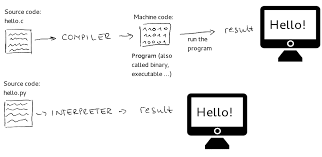
\includegraphics[width=0.7\linewidth]{index.png}
\caption{Interpreted vs compiled language}
\end{figure}

As a result, \(\tt{python}\) is essentially an \emph{interactive} programming language, you can program and see the results almost at the same time. This is very nice for a faster development since compilation time can be quite long (just to give an idea the compilation of our \texttt{C++} financial code takes more than one hour).
However there are drawbacks in terms of performance, the \emph{translation} to machine language has to be done in real-time resulting in slower execution times.

\begin{figure}[h]
\centering
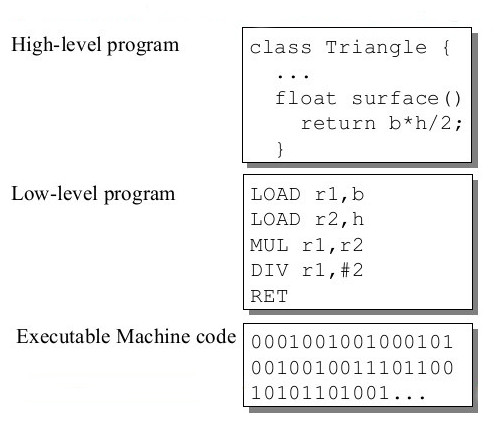
\includegraphics[width=0.5\linewidth]{machine_language.jpeg}
\caption{Human readable vs machine code}
\end{figure}

In the next chapters we'll take a quick tour of $\tt{python}$ and see the main features and characteristics of this programming language, later on we will see how it can be useful to solve real-world finance problems.

First of all since $\tt{python}$, as basically all programs, comes in different version and flavours we need to specify the particular one we are going to use.
The latest version (at the time I'm wrtiting this pages) is \(\tt{3.8.5}\), but it is continously evolving, however it is not difficult to see older versions floating around (e.g. \(\tt{2.7}\)).
This is because there are some big differences between \(\tt{python 2.X}\) and \(\tt{python 3.X}\) which prevent a sizeable portion of \(\tt{python 2}\) users to stick with it (consider that moving to \(\tt{python 3}\) would require a large amount of work to adapt big projects).
In conclusion we will concentrate on \textbf{\(\tt{python 3.7}\)}.

\section{$\tt{Python}$ basics}\label{python-basics}

Every language has \emph{keywords}, these are reserved words that have a special meaning and tell the computer what to do. The first one we encounter is \(\tt{print}\): it prints to screen whatever is specified between the parenthesis.

\begin{tcolorbox}[breakable, size=fbox, boxrule=1pt, pad at break*=1mm, colback=cellbackground, colframe=cellborder]
\begin{Verbatim}[commandchars=\\\{\}]
\PY{n+nb}{print} \PY{p}{(}\PY{l+s+s2}{\PYZdq{}}\PY{l+s+s2}{Hello world !}\PY{l+s+s2}{\PYZdq{}}\PY{p}{)} 

Hello world !
\end{Verbatim}
\end{tcolorbox}

\begin{tcolorbox}[breakable, size=fbox, boxrule=1pt, pad at break*=1mm, colback=cellbackground, colframe=cellborder]
\begin{Verbatim}[commandchars=\\\{\}]
\PY{n+nb}{print} \PY{p}{(}\PY{l+s+s2}{\PYZdq{}}\PY{l+s+s2}{Welcome}\PY{l+s+s2}{\PYZdq{}}\PY{p}{)}
\PY{n+nb}{print} \PY{p}{(}\PY{l+s+s2}{\PYZdq{}}\PY{l+s+s2}{to}\PY{l+s+s2}{\PYZdq{}}\PY{p}{)}
\PY{n+nb}{print} \PY{p}{(}\PY{l+s+s2}{\PYZdq{}}\PY{l+s+s2}{everybody}\PY{l+s+s2}{\PYZdq{}}\PY{p}{)}

Welcome
to
everybody
\end{Verbatim}
\end{tcolorbox}

Good programming practice recommends to document the code you write (you will soon see that it is surprisingly easy to forget what you wanted to do in your code). In \(\tt{python}\) you can add comments to code starting a line with a hash character (\#).

\begin{tcolorbox}[breakable, size=fbox, boxrule=1pt, pad at break*=1mm, colback=cellbackground, colframe=cellborder]
\begin{Verbatim}[commandchars=\\\{\}]
\PY{n+nb}{print} \PY{p}{(}\PY{l+s+s2}{\PYZdq{}}\PY{l+s+s2}{Ciao}\PY{l+s+s2}{\PYZdq{}}\PY{p}{)} \PY{c+c1}{\PYZsh{} this is a comment}

Ciao
\end{Verbatim}
\end{tcolorbox}

\subsection{Variables}\label{variables}

A variable is a computer memory location paired with an associated symbolic name, which contains some quantity of information referred to as a *value* (e.g.~a number, a string\ldots{}). Variables and hence data they contain, can be used, referenced and manipulated throughout a program.
A value is assigned to a variable with the equal operator (=). 

\begin{figure}[h]
\centering
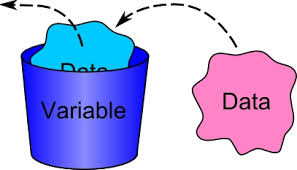
\includegraphics[width=0.5\linewidth]{var1.jpeg}
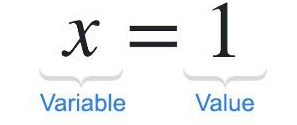
\includegraphics[width=0.5\linewidth]{var2.jpeg}
\caption{Graphical representation of a variable.}
\end{figure}

\begin{tcolorbox}[breakable, size=fbox, boxrule=1pt, pad at break*=1mm, colback=cellbackground, colframe=cellborder]
\begin{Verbatim}[commandchars=\\\{\}]
\PY{n}{x} \PY{o}{=} \PY{l+m+mi}{9}
\PY{n+nb}{print} \PY{p}{(}\PY{n}{x}\PY{p}{)}

9
\end{Verbatim}
\end{tcolorbox}

\begin{tcolorbox}[breakable, size=fbox, boxrule=1pt, pad at break*=1mm, colback=cellbackground, colframe=cellborder]
\begin{Verbatim}[commandchars=\\\{\}]
\PY{n}{myphone} \PY{o}{=} \PY{l+s+s2}{\PYZdq{}}\PY{l+s+s2}{Huawei P10Lite}\PY{l+s+s2}{\PYZdq{}}
\PY{n+nb}{print} \PY{p}{(}\PY{n}{myphone}\PY{p}{)}

Huawei P10Lite
\end{Verbatim}
\end{tcolorbox}

Another very useful keyword is \(\tt{type}\): it tells which kind of object is stored in a variable.

\begin{tcolorbox}[breakable, size=fbox, boxrule=1pt, pad at break*=1mm, colback=cellbackground, colframe=cellborder]
\begin{Verbatim}[commandchars=\\\{\}]
\PY{n+nb}{print} \PY{p}{(}\PY{n+nb}{type}\PY{p}{(}\PY{n}{x}\PY{p}{)}\PY{p}{)}
\PY{n+nb}{print} \PY{p}{(}\PY{n+nb}{type}\PY{p}{(}\PY{n}{myphone}\PY{p}{)}\PY{p}{)}

<class 'int'>
<class 'str'>
\end{Verbatim}
\end{tcolorbox}

After their definitions \(\tt{x}\) and \(\tt{myphone}\) can be used as aliases for a number and a string and their content manipulated, for example:

\begin{tcolorbox}[breakable, size=fbox, boxrule=1pt, pad at break*=1mm, colback=cellbackground, colframe=cellborder]
\begin{Verbatim}[commandchars=\\\{\}]
\PY{n+nb}{print} \PY{p}{(}\PY{n}{x}\PY{o}{+}\PY{l+m+mi}{5}\PY{p}{)}

14
\end{Verbatim}
\end{tcolorbox}

There are rules that limit the variable naming possibilities, in particular they must:
\begin{itemize}
\item begin with a letter (\tt{myphone}) or underscore (\tt{\_myphone});
\item other characters can be letters, numbers or more \_;
\item variable names are case-sensitive so \tt{myphone} and \tt{myPhone} are two distinct variables;
\end{itemize}

\textbf{Keywords, as said, are reserved words and as such cannot be used as variable names (e.g.~\(\tt{print, type, for...}\))}.

To use \textbf{good} variable names (and make you programs clearer and easier to read) always choose meaningful names instead of short names (i.e. \(\tt{numberOfCakes}\) is much better than simply \(\tt{n}\)), try to be consistent with your conventions (e.g.~choose once and for all between \(\tt{number\_of\_cakes}\) or
\(\tt{numberofcakes}\) or \(\tt{numberOfCakes}\)), usually begin a variable name with underscore (\_) only for a special case (will see later when this is usually done).

\subsection{Boolean expressions}\label{boolean-expressions}

Boolean expressions evaluate to \(\tt{true}\) or \(\tt{false}\) only. This type
of expressions usually involve logical or comparison operators like \(\tt{or}\), \(\tt{and}\), \textgreater{} (greater than), \textless{} (less than)\ldots{}
The equal boolean operator symbol is a double = (==), to not be confused with the assignement operator single = (=), with the first we compare two variables, with the second we associate a value to a variable.

Let's see some example. The following expression answer the question is 1 equal to 2:

\begin{tcolorbox}[breakable, size=fbox, boxrule=1pt, pad at break*=1mm, colback=cellbackground, colframe=cellborder]
\begin{Verbatim}[commandchars=\\\{\}]
\PY{l+m+mi}{1} \PY{o}{==} \PY{l+m+mi}{2} 

False
\end{Verbatim}
\end{tcolorbox}

Here another example using the not equal operator (!=):

\begin{tcolorbox}[breakable, size=fbox, boxrule=1pt, pad at break*=1mm, colback=cellbackground, colframe=cellborder]
\begin{Verbatim}[commandchars=\\\{\}]

True
\end{Verbatim}
\end{tcolorbox}

\begin{tcolorbox}[breakable, size=fbox, boxrule=1pt, pad at break*=1mm, colback=cellbackground, colframe=cellborder]
\begin{Verbatim}[commandchars=\\\{\}]
\PY{l+m+mi}{2} \PY{o}{\PYZlt{}} \PY{l+m+mi}{2}

False
\end{Verbatim}
\end{tcolorbox}

\begin{tcolorbox}[breakable, size=fbox, boxrule=1pt, pad at break*=1mm, colback=cellbackground, colframe=cellborder]
\begin{Verbatim}[commandchars=\\\{\}]
\PY{l+m+mi}{2} \PY{o}{\PYZlt{}}\PY{o}{=} \PY{l+m+mi}{2}  \PY{c+c1}{\PYZsh{} in this case we allow the numbers to be equal too}

True
\end{Verbatim}
\end{tcolorbox}

\begin{tcolorbox}[breakable, size=fbox, boxrule=1pt, pad at break*=1mm, colback=cellbackground, colframe=cellborder]
\begin{Verbatim}[commandchars=\\\{\}]
\PY{n+nb}{print} \PY{p}{(}\PY{n}{x}\PY{p}{)}
\PY{l+m+mi}{15} \PY{o}{\PYZlt{}}\PY{o}{=} \PY{n}{x} \PY{o+ow}{and} \PY{n}{x} \PY{o}{\PYZlt{}}\PY{o}{=} \PY{l+m+mi}{20} \PY{c+c1}{\PYZsh{} this expression could also be written as 15 \PYZlt{}= x \PYZlt{}= 20}

11
False
\end{Verbatim}
\end{tcolorbox}

\begin{tcolorbox}[breakable, size=fbox, boxrule=1pt, pad at break*=1mm, colback=cellbackground, colframe=cellborder]            
\begin{Verbatim}[commandchars=\\\{\}]
\PY{l+m+mi}{15} \PY{o}{\PYZlt{}}\PY{o}{=} \PY{n}{x} \PY{o+ow}{or} \PY{n}{x} \PY{o}{\PYZlt{}}\PY{o}{=} \PY{l+m+mi}{20}

True
\end{Verbatim}
\end{tcolorbox}

\begin{tcolorbox}[breakable, size=fbox, boxrule=1pt, pad at break*=1mm, colback=cellbackground, colframe=cellborder]            
\begin{Verbatim}[commandchars=\\\{\}]
\PY{o+ow}{not} \PY{p}{(}\PY{n}{x} \PY{o}{\PYZgt{}} \PY{l+m+mi}{20}\PY{p}{)} \PY{c+c1}{\PYZsh{} the not keyword negates the following expression}

True
\end{Verbatim}
\end{tcolorbox}

\subsection{String expressions}\label{string-expressions}

A ``string'' is a sequence of characters (letters, digits, spaces, punctuation\ldots{}). There are many operations that can be performed on strings, like for example concatenate (with + operator), truncate, replace characters\ldots{}

\begin{tcolorbox}[breakable, size=fbox, boxrule=1pt, pad at break*=1mm, colback=cellbackground, colframe=cellborder]            
\begin{Verbatim}[commandchars=\\\{\}]
\PY{n}{mystring} \PY{o}{=} \PY{l+s+s2}{\PYZdq{}}\PY{l+s+s2}{some text with punctuation, spaces and digits 10}\PY{l+s+s2}{\PYZdq{}}
\PY{n}{mystring}\PY{o}{.}\PY{n}{replace}\PY{p}{(}\PY{l+s+s2}{\PYZdq{}}\PY{l+s+s2}{s}\PY{l+s+s2}{\PYZdq{}}\PY{p}{,} \PY{l+s+s2}{\PYZdq{}}\PY{l+s+s2}{z}\PY{l+s+s2}{\PYZdq{}}\PY{p}{)}

'zome text with punctuation, zpacez and digitz 10'
\end{Verbatim}
\end{tcolorbox}

\begin{tcolorbox}[breakable, size=fbox, boxrule=1pt, pad at break*=1mm, colback=cellbackground, colframe=cellborder]            
\begin{Verbatim}[commandchars=\\\{\}]
\PY{l+s+s2}{\PYZdq{}}\PY{l+s+s2}{abc}\PY{l+s+s2}{\PYZdq{}} \PY{o}{+} \PY{l+s+s2}{\PYZdq{}}\PY{l+s+s2}{def}\PY{l+s+s2}{\PYZdq{}} \PY{c+c1}{\PYZsh{} it is possible to concatenate strings with + }

'abcdef'
\end{Verbatim}
\end{tcolorbox}

\begin{tcolorbox}[breakable, size=fbox, boxrule=1pt, pad at break*=1mm, colback=cellbackground, colframe=cellborder]            
\begin{Verbatim}[commandchars=\\\{\}]
\PY{l+s+s2}{\PYZdq{}}\PY{l+s+s2}{The number }\PY{l+s+s2}{\PYZdq{}} \PY{o}{+} \PY{l+m+mi}{4} \PY{o}{+} \PY{l+s+s2}{\PYZdq{}}\PY{l+s+s2}{ is my favourite number}\PY{l+s+s2}{\PYZdq{}}
\PY{c+c1}{\PYZsh{} this causes an error since we are trying to concatenate a string }
\PY{c+c1}{\PYZsh{} with a number so two different kind of objects}

---------------------------------------------------------------------------

TypeError                                 Traceback (most recent call last)

<ipython-input-33-b9f65c5a45f7> in <module>()
----> 1 "The number " + 4 + " is my favourite number"
      2 \# this causes an error since we are trying to concatenate a string
      3 \# with a number so two different kind of objects

TypeError: can only concatenate str (not "int") to str
\end{Verbatim}
\end{tcolorbox}

To avoid this error is possible to \textbf{cast} an object to a different type which means to convert an object to a different type. In this case we can \emph{force} the number four to be represented as a string with the \(\tt{str()}\) function:

\begin{tcolorbox}[breakable, size=fbox, boxrule=1pt, pad at break*=1mm, colback=cellbackground, colframe=cellborder]            
\begin{Verbatim}[commandchars=\\\{\}]
\PY{l+s+s2}{\PYZdq{}}\PY{l+s+s2}{The number }\PY{l+s+s2}{\PYZdq{}} \PY{o}{+} \PY{n+nb}{str}\PY{p}{(}\PY{l+m+mi}{4}\PY{p}{)} \PY{o}{+} \PY{l+s+s2}{\PYZdq{}}\PY{l+s+s2}{ is my favourite number}\PY{l+s+s2}{\PYZdq{}}

'The number 4 is my favourite number'
\end{Verbatim}
\end{tcolorbox}

\begin{tcolorbox}[breakable, size=fbox, boxrule=1pt, pad at break*=1mm, colback=cellbackground, colframe=cellborder]            
\begin{Verbatim}[commandchars=\\\{\}]
\PY{n+nb}{print} \PY{p}{(}\PY{n+nb}{type}\PY{p}{(}\PY{l+m+mf}{3.4}\PY{p}{)}\PY{p}{)}
\PY{n+nb}{print} \PY{p}{(}\PY{n+nb}{type}\PY{p}{(}\PY{n+nb}{str}\PY{p}{(}\PY{l+m+mf}{3.4}\PY{p}{)}\PY{p}{)}\PY{p}{)}

<class 'float'>
<class 'str'>
\end{Verbatim}
\end{tcolorbox}

In this simple case everything worked fine but type casting is not always possible: for example a number can be converted to a string (e.g.~from the integer 4 to the actual symbol ``4'') but the opposite is not possible (e.g.~cannot convert the string ``matteo'' to a meaningful number). In this second case we can try to use the function \(\tt{int()}\) to convert a string to an integer.

\begin{tcolorbox}[breakable, size=fbox, boxrule=1pt, pad at break*=1mm, colback=cellbackground, colframe=cellborder]            
\begin{Verbatim}[commandchars=\\\{\}]
\PY{n+nb}{int}\PY{p}{(}\PY{l+s+s2}{\PYZdq{}}\PY{l+s+s2}{matteo}\PY{l+s+s2}{\PYZdq{}}\PY{p}{)}

---------------------------------------------------------------------------

ValueError                                Traceback (most recent call last)

<ipython-input-17-979283bb65e4> in <module>
----> 1 int("matteo")  

ValueError: invalid literal for int() with base 10: 'matteo'
\end{Verbatim}
\end{tcolorbox}

\begin{tcolorbox}[breakable, size=fbox, boxrule=1pt, pad at break*=1mm, colback=cellbackground, colframe=cellborder]            
\begin{Verbatim}[commandchars=\\\{\}]
\PY{n+nb}{int}\PY{p}{(}\PY{l+s+s2}{\PYZdq{}}\PY{l+s+s2}{4}\PY{l+s+s2}{\PYZdq{}}\PY{p}{)}

4
\end{Verbatim}
\end{tcolorbox}

\paragraph{Pretty string formatting: } in order to get prettier strings than those obtained just concatenating with the + operator, \(\tt{python}\) allows to format text using the following syntax ``text {} other text''.format(variable).
With this notation, each {} is mapped to the variables listed in the $\tt{format}$ statement, the optional characters inside the curly brackets can determine the resulting format, for example in the following code $\tt{:.1f}$ means that this variable is float number and that has to be printed with 1 digit only after the decimal separator. 

\begin{tcolorbox}[breakable, size=fbox, boxrule=1pt, pad at break*=1mm, colback=cellbackground, colframe=cellborder]            
\begin{Verbatim}[commandchars=\\\{\}]
\PY{l+s+s2}{\PYZdq{}}\PY{l+s+s2}{The speed of light is about }\PY{l+s+si}{\PYZob{}:.1f\PYZcb{}}\PY{l+s+s2}{ }\PY{l+s+si}{\PYZob{}\PYZcb{}}\PY{l+s+s2}{\PYZdq{}}\PY{o}{.}\PY{n}{format}\PY{p}{(}\PY{l+m+mf}{299792.458}\PY{p}{,} \PY{l+s+s2}{\PYZdq{}}\PY{l+s+s2}{km/s}\PY{l+s+s2}{\PYZdq{}}\PY{p}{)}

'The speed of light is about 299792.5 km/s'
\end{Verbatim}
\end{tcolorbox}

In addition $\tt{format}$ allows for 0-padding of numbers, left or right alignement of text columns and so on.

\subsection{Mathematical expressions}\label{mathematical-expressions}

Below few examples of the basic mathematical expressions available in $\tt{python}$.

\begin{tcolorbox}[breakable, size=fbox, boxrule=1pt, pad at break*=1mm, colback=cellbackground, colframe=cellborder]            
\begin{Verbatim}[commandchars=\\\{\}]
\PY{l+m+mi}{1} \PY{o}{+} \PY{l+m+mi}{2}

3
\end{Verbatim}
\end{tcolorbox}

\begin{tcolorbox}[breakable, size=fbox, boxrule=1pt, pad at break*=1mm, colback=cellbackground, colframe=cellborder]            
\begin{Verbatim}[commandchars=\\\{\}]
\PY{l+m+mi}{40} \PY{o}{\PYZhy{}} \PY{l+m+mi}{5}

35
\end{Verbatim}
\end{tcolorbox}

\begin{tcolorbox}[breakable, size=fbox, boxrule=1pt, pad at break*=1mm, colback=cellbackground, colframe=cellborder]            
\begin{Verbatim}[commandchars=\\\{\}]
\PY{n}{x} \PY{o}{*} \PY{l+m+mi}{20} \PY{c+c1}{\PYZsh{} remember that we set x equal to 9}

180
\end{Verbatim}
\end{tcolorbox}

\begin{tcolorbox}[breakable, size=fbox, boxrule=1pt, pad at break*=1mm, colback=cellbackground, colframe=cellborder]            
\begin{Verbatim}[commandchars=\\\{\}]
\PY{n}{x} \PY{o}{/} \PY{l+m+mi}{4}

2.25
\end{Verbatim}
\end{tcolorbox}

\begin{tcolorbox}[breakable, size=fbox, boxrule=1pt, pad at break*=1mm, colback=cellbackground, colframe=cellborder]            
\begin{Verbatim}[commandchars=\\\{\}]
\PY{n+nb}{print} \PY{p}{(}\PY{n+nb}{type}\PY{p}{(}\PY{l+m+mf}{2.25}\PY{p}{)}\PY{p}{)}

<class 'float'>
\end{Verbatim}
\end{tcolorbox}

\begin{tcolorbox}[breakable, size=fbox, boxrule=1pt, pad at break*=1mm, colback=cellbackground, colframe=cellborder]            
\begin{Verbatim}[commandchars=\\\{\}]
\PY{n}{x} \PY{o}{/}\PY{o}{/} \PY{l+m+mi}{4} \PY{c+c1}{\PYZsh{} interger division \PYZhy{} result will be truncated to the }
       \PY{c+c1}{\PYZsh{} corresponding integer (no rounding)}
       \PY{c+c1}{\PYZsh{} 11 / 3 = 3.666666 \PYZhy{}\PYZgt{} 11 // 3 = 3}

2
\end{Verbatim}
\end{tcolorbox}

\begin{tcolorbox}[breakable, size=fbox, boxrule=1pt, pad at break*=1mm, colback=cellbackground, colframe=cellborder]            
\begin{Verbatim}[commandchars=\\\{\}]
\PY{n}{y} \PY{o}{=} \PY{l+m+mi}{3}
\PY{n}{x} \PY{o}{*}\PY{o}{*} \PY{n}{y} \PY{c+c1}{\PYZsh{} x to the power of y}

729
\end{Verbatim}
\end{tcolorbox}

\begin{tcolorbox}[breakable, size=fbox, boxrule=1pt, pad at break*=1mm, colback=cellbackground, colframe=cellborder]            
\begin{Verbatim}[commandchars=\\\{\}]
\PY{l+m+mi}{3} \PY{o}{*} \PY{p}{(}\PY{n}{x} \PY{o}{+} \PY{n}{y}\PY{p}{)}

36
\end{Verbatim}
\end{tcolorbox}

As an example of variable manipulation let's try to increment \(\tt{x}\) by 1 and save the result again in \(\tt{x}\).

\begin{tcolorbox}[breakable, size=fbox, boxrule=1pt, pad at break*=1mm, colback=cellbackground, colframe=cellborder]            
\begin{Verbatim}[commandchars=\\\{\}]
\PY{n+nb}{print} \PY{p}{(}\PY{n}{x}\PY{p}{)}
\PY{n}{x} \PY{o}{=} \PY{n}{x} \PY{o}{+} \PY{l+m+mi}{1}
\PY{n+nb}{print} \PY{p}{(}\PY{n}{x}\PY{p}{)}

15
16
\end{Verbatim}
\end{tcolorbox}

Sometimes the increment of a variable plus the assignment to the same variable is written with a more compact syntax \texttt{x += 1} (this is also true for other operators e.g. \texttt{x *= 2}).

More complex mathematical functions are not directly available, let's see for example the logarithm:

\begin{tcolorbox}[breakable, size=fbox, boxrule=1pt, pad at break*=1mm, colback=cellbackground, colframe=cellborder]            
\begin{Verbatim}[commandchars=\\\{\}]
\PY{n}{log}\PY{p}{(}\PY{l+m+mi}{3}\PY{p}{)}

---------------------------------------------------------------------------

NameError                                 Traceback (most recent call last)

<ipython-input-17-ffde4d60496a> in <module>()
    ----> 1 log(3) \# causes an error because the logarithm function
          2        \# is not available by default


NameError: name 'log' is not defined
\end{Verbatim}
\end{tcolorbox}

\section{Modules}\label{modules}

One very important feature of each language is the ability to reuse code among different programs, e.g.~imagine how awful would be if you had to reimplement every time you need it a function to compute the logarithm.
Usually there are mechanisms that allow to collect useful routines in \emph{packages} (or \emph{libraries}, or \emph{modules}) so that later they can be called and used by any program may need them.

These collections of utilities in \(\tt{python}\) are called \emph{modules} and each installation of this language brings with it a standard set of them. If you need more functionality, you can download more modules from the web (there are zillions out there) or if you are not satisfied with what you found you can write your own (which is one the goal of this course in the end).

Some examples of useful modules we will use are:

\begin{itemize}
\tightlist
\item
  Numpy - which provides matrix algebra functionality and much more;
\item
  Scipy - which provides a whole series of scientific computing
  functions;
\item
  Pandas - which provides tools for manipulating time series or dataset
  in general;
\item
  Matplotlib - for plotting graphs;
\item
  Jupyter - for notebooks like this one.
\end{itemize}

\begin{figure}
\centering
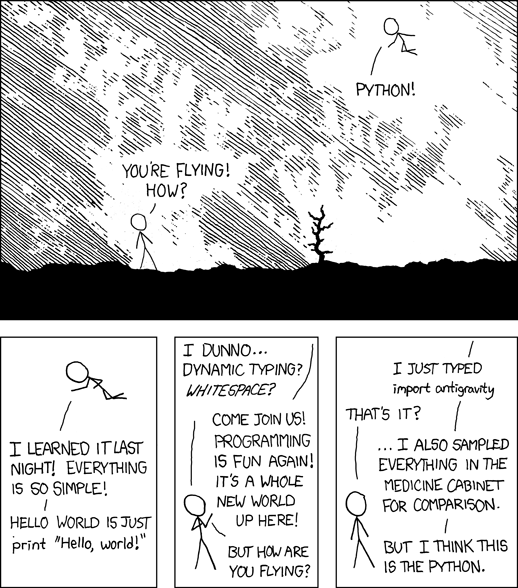
\includegraphics[width=0.75\linewidth]{python.png}
\caption{$\tt{Python}$ has many modules for download on the web\ldots{}}
\end{figure}

Later we will take a closer look at three modules which are quite useful in financial analysis.

In order to load a module in a \(\tt{python}\) program you can use the \(\tt{import}\) keyword. To inspect a module (to understand which are its functionalities) it can be used the \(\tt{help}\) and \(\tt{dir}\) keywords: the first write a help message which usually describes the functionalities of a module, the latter list all the available functions of a module.
\textbf{In order to access a function of a module you have to use the . (dot) operator: module-name.function-name.}

Let's see an example dealing with the\(\tt{math}\) module which implements the most common mathematical functions.

\begin{tcolorbox}[breakable, size=fbox, boxrule=1pt, pad at break*=1mm, colback=cellbackground, colframe=cellborder]            
\begin{Verbatim}[commandchars=\\\{\}]
\PY{k+kn}{import} \PY{n+nn}{math}
\PY{n+nb}{dir}\PY{p}{(}\PY{n}{math}\PY{p}{)}

{\color{outcolor}Out[{\color{outcolor}18}]:} ['\_\_doc\_\_',
          '\_\_loader\_\_',
          '\_\_name\_\_',
          '\_\_package\_\_',
          '\_\_spec\_\_',
          'acos',
          'acosh',
          'asin',
          'asinh',
          'atan',
          'atan2',
          'atanh',
          'ceil',
          'copysign',
          'cos',
          'cosh',
...
\end{Verbatim}
\end{tcolorbox}

\begin{tcolorbox}[breakable, size=fbox, boxrule=1pt, pad at break*=1mm, colback=cellbackground, colframe=cellborder]            
\begin{Verbatim}[commandchars=\\\{\}]
\PY{n+nb}{help}\PY{p}{(}\PY{n}{math}\PY{p}{)}

Help on module math:

NAME
    math

MODULE REFERENCE
    https://docs.python.org/3.6/library/math

    The following documentation is automatically generated from the Python
    source files.  It may be incomplete, incorrect or include features that
    are considered implementation detail and may vary between Python
    implementations.  When in doubt, consult the module reference at the
    location listed above.

DESCRIPTION
    This module is always available.  It provides access to the
    mathematical functions defined by the C standard.

FUNCTIONS
    acos({\ldots})
        acos(x)

        Return the arc cosine (measured in radians) of x.
...
\end{Verbatim}
\end{tcolorbox}

\begin{tcolorbox}[breakable, size=fbox, boxrule=1pt, pad at break*=1mm, colback=cellbackground, colframe=cellborder]            
\begin{Verbatim}[commandchars=\\\{\}]
\PY{n}{math}\PY{o}{.}\PY{n}{log}\PY{p}{(}\PY{l+m+mi}{3}\PY{p}{)}

1.0986122886681098
\end{Verbatim}
\end{tcolorbox}

\begin{tcolorbox}[breakable, size=fbox, boxrule=1pt, pad at break*=1mm, colback=cellbackground, colframe=cellborder]            
\begin{Verbatim}[commandchars=\\\{\}]
\PY{n}{math}\PY{o}{.}\PY{n}{exp}\PY{p}{(}\PY{l+m+mi}{3}\PY{p}{)}

20.085536923187668
\end{Verbatim}
\end{tcolorbox}

\begin{tcolorbox}[breakable, size=fbox, boxrule=1pt, pad at break*=1mm, colback=cellbackground, colframe=cellborder]            
\begin{Verbatim}[commandchars=\\\{\}]
\PY{n+nb}{print} \PY{p}{(}\PY{n+nb}{type}\PY{p}{(}\PY{n}{math}\PY{o}{.}\PY{n}{log}\PY{p}{)}\PY{p}{)} \PY{c+c1}{\PYZsh{} yet another type: builtin function}
\PY{n+nb}{print} \PY{p}{(}\PY{n+nb}{type}\PY{p}{(}\PY{n}{math}\PY{o}{.}\PY{n}{log}\PY{p}{(}\PY{l+m+mi}{3}\PY{p}{)}\PY{p}{)}\PY{p}{)}

<class 'builtin\_function\_or\_method'>
<class 'float'>
\end{Verbatim}
\end{tcolorbox}

If we want to avoid to type ``math.'' every time we compute a logarithm or an exponential, we can just import the needed functions from a module using the following syntax:

\begin{tcolorbox}[breakable, size=fbox, boxrule=1pt, pad at break*=1mm, colback=cellbackground, colframe=cellborder]            
\begin{Verbatim}[commandchars=\\\{\}]
\PY{k+kn}{from} \PY{n+nn}{math} \PY{k}{import} \PY{n}{log}\PY{p}{,} \PY{n}{exp}
\PY{n+nb}{print} \PY{p}{(}\PY{n}{log}\PY{p}{(}\PY{l+m+mi}{3}\PY{p}{)}\PY{p}{)}
\PY{n+nb}{print} \PY{p}{(}\PY{n}{exp}\PY{p}{(}\PY{l+m+mi}{3}\PY{p}{)}\PY{p}{)}

1.0986122886681098
20.085536923187668
\end{Verbatim}
\end{tcolorbox}

As an example let's compute the interest rate \(r\) that produces a return \(R\) of 11000 Euro when investing 10000 Euro for 2 years:

\(R = N\mathrm{e}^{r\tau} \rightarrow r = \frac{1}{\tau} \mathrm{log}(\frac{R}{N})\)

\begin{tcolorbox}[breakable, size=fbox, boxrule=1pt, pad at break*=1mm, colback=cellbackground, colframe=cellborder]            
\begin{Verbatim}[commandchars=\\\{\}]
\PY{n}{rate} \PY{o}{=} \PY{p}{(}\PY{l+m+mi}{1}\PY{o}{/}\PY{l+m+mi}{2}\PY{p}{)}\PY{o}{*}\PY{n}{log}\PY{p}{(}\PY{l+m+mf}{11000}\PY{o}{/}\PY{l+m+mi}{10000}\PY{p}{)}
\PY{n+nb}{print} \PY{p}{(}\PY{n}{rate}\PY{p}{)}

0.04765508990216247
\end{Verbatim}
\end{tcolorbox}

\section{Indented blocks and the $\tt{if/else}$ statement}\label{indented-blocks-and-the-ttifelse-statement}

Unlike other languages which uses parenthesis to isolate blocks of code $\tt{python}$ uses indentation. A first example of this is given by $\tt{if/then}$ statements. Such commands allow to dynamically run different blocks of code based on certain conditions. For example in the following we print different statements according to the value of $\tt{x}$, note the that the block of code to be run according each condition is shifted (i.e.~indented) with respect to the rest of the
code:

\begin{tcolorbox}[breakable, size=fbox, boxrule=1pt, pad at break*=1mm, colback=cellbackground, colframe=cellborder]            
\begin{Verbatim}[commandchars=\\\{\}]
\PY{n+nb}{print} \PY{p}{(}\PY{n}{x}\PY{p}{)}
\PY{k}{if} \PY{n}{x} \PY{o}{==} \PY{l+m+mi}{1}\PY{p}{:} 
    \PY{n+nb}{print} \PY{p}{(}\PY{l+s+s2}{\PYZdq{}}\PY{l+s+s2}{This will not be printed}\PY{l+s+s2}{\PYZdq{}}\PY{p}{)} 
    \PY{c+c1}{\PYZsh{} the block of code that is run if the first condition is met is indented}
\PY{k}{elif} \PY{n}{x} \PY{o}{==} \PY{l+m+mi}{15}\PY{p}{:}
    \PY{n+nb}{print} \PY{p}{(}\PY{l+s+s2}{\PYZdq{}}\PY{l+s+s2}{This will not be printed either}\PY{l+s+s2}{\PYZdq{}}\PY{p}{)}
    \PY{c+c1}{\PYZsh{} again the block of code that is run here is indented}
    \PY{c+c1}{\PYZsh{} to be \PYZdq{}isolated\PYZdq{} by the rest }
\PY{k}{else}\PY{p}{:}
    \PY{n+nb}{print} \PY{p}{(}\PY{l+s+s2}{\PYZdq{}}\PY{l+s+s2}{This *will* be printed}\PY{l+s+s2}{\PYZdq{}}\PY{p}{)}

16
This *will* be printed
\end{Verbatim}
\end{tcolorbox}

If by mistake the indentation of a block is missing an error is raised:
\begin{tcolorbox}[breakable, size=fbox, boxrule=1pt, pad at break*=1mm, colback=cellbackground, colframe=cellborder]            
\begin{Verbatim}[commandchars=\\\{\}]
\PY{k}{if} \PY{n}{x} \PY{o}{==} \PY{l+m+mi}{1}\PY{p}{:} 
\PY{n+nb}{print} \PY{p}{(}\PY{l+s+s2}{\PYZdq{}}\PY{l+s+s2}{This will not be printed}\PY{l+s+s2}{\PYZdq{}}\PY{p}{)}
\PY{k}{elif} \PY{n}{x} \PY{o}{==} \PY{l+m+mi}{15}\PY{p}{:}
    \PY{n+nb}{print} \PY{p}{(}\PY{l+s+s2}{\PYZdq{}}\PY{l+s+s2}{This will not be printed either}\PY{l+s+s2}{\PYZdq{}}\PY{p}{)}
\PY{k}{else}\PY{p}{:}
    \PY{n+nb}{print} \PY{p}{(}\PY{l+s+s2}{\PYZdq{}}\PY{l+s+s2}{This *will* be printed}\PY{l+s+s2}{\PYZdq{}}\PY{p}{)}

File "<ipython-input-38-4535a45a6419>", line 3
  print ("This will not be printed")
    \^{}
IndentationError: expected an indented block
\end{Verbatim}
\end{tcolorbox}

Below another example:
\begin{tcolorbox}[breakable, size=fbox, boxrule=1pt, pad at break*=1mm, colback=cellbackground, colframe=cellborder]            
\begin{Verbatim}[commandchars=\\\{\}]
\PY{k}{if} \PY{n}{x} \PY{o}{!=} \PY{l+m+mi}{1}\PY{p}{:}
   \PY{n+nb}{print} \PY{p}{(}\PY{l+s+s2}{\PYZdq{}}\PY{l+s+s2}{x does not equal to 1}\PY{l+s+s2}{\PYZdq{}}\PY{p}{)}

x does not equal to 1
\end{Verbatim}
\end{tcolorbox}

Just for comparison this is the same code written in $\tt{C++}$:

\begin{Shaded}
\begin{Highlighting}[]
\ControlFlowTok{if}\NormalTok{ (x == }\DecValTok{1}\NormalTok{) \{}
\NormalTok{ print (}\StringTok{"This will not be printed"}\NormalTok{);}
\NormalTok{\}}
\ControlFlowTok{else} \ControlFlowTok{if}\NormalTok{ (x == }\DecValTok{15}\NormalTok{) \{}
\NormalTok{  print (}\StringTok{"This will not be printed either"}\NormalTok{);}
\NormalTok{\}}
\ControlFlowTok{else}\NormalTok{ \{}
\NormalTok{print (}\StringTok{"This *will* be printed"}\NormalTok{);}
\NormalTok{\}}
\end{Highlighting}
\end{Shaded}

N.B. Notice how indentation doesn't matter at all here since the blocks are enclosed and defined by the brackets.

\section{Loops}\label{loops}

Another very important feature of a language is the ability to repeatedly run the same block of code many times. These is called looping and in \(\tt{python}\) can be done with $\tt{for}$ or $\tt{while}$ keywords.

\subsection{for}\label{for}

In a $\tt{for}$ loop we specifiy the set (or interval) over which we want to loop and a variable will assume all the values in that set (or interval). For example let's assume we want to print all the numbers between 25 and 30 excluded (here the keyword $\tt{range}$ returns the list of integers between the specified limits, if the first limit is not specified 0 is assumed):

\begin{tcolorbox}[breakable, size=fbox, boxrule=1pt, pad at break*=1mm, colback=cellbackground, colframe=cellborder]            
\begin{Verbatim}[commandchars=\\\{\}]
\PY{k}{for} \PY{n}{i} \PY{o+ow}{in} \PY{n+nb}{range}\PY{p}{(}\PY{l+m+mi}{25}\PY{p}{,} \PY{l+m+mi}{30}\PY{p}{)}\PY{p}{:}
     \PY{n+nb}{print} \PY{p}{(}\PY{n}{i}\PY{p}{)}

25
26
27
28
29
\end{Verbatim}
\end{tcolorbox}

At each cycle of the loop the variable $\tt{i}$ takes one of the values between
25 and 31. With $\tt{range}$ it is also possible to specify the step, so that the loop can jump every 2 units or to go in descending order:

\begin{tcolorbox}[breakable, size=fbox, boxrule=1pt, pad at break*=1mm, colback=cellbackground, colframe=cellborder]            
\begin{Verbatim}[commandchars=\\\{\}]
\PY{k}{for} \PY{n}{i} \PY{o+ow}{in} \PY{n+nb}{range} \PY{p}{(}\PY{l+m+mi}{30}\PY{p}{,} \PY{l+m+mi}{25}\PY{p}{,} \PY{o}{\PYZhy{}}\PY{l+m+mi}{1}\PY{p}{)}\PY{p}{:}
    \PY{n+nb}{print} \PY{p}{(}\PY{n}{i}\PY{p}{)}

30
29
28
27
26
\end{Verbatim}
\end{tcolorbox}

If it is needed to skip values in the loop the $\tt{continue}$ keyword can be used; in the code below 5 is actually missing from the list in the printout since it has been skipped by the $\tt{continue}$:

\begin{tcolorbox}[breakable, size=fbox, boxrule=1pt, pad at break*=1mm, colback=cellbackground, colframe=cellborder]            
\begin{Verbatim}[commandchars=\\\{\}]
\PY{k}{for} \PY{n}{i} \PY{o+ow}{in} \PY{n+nb}{range}\PY{p}{(}\PY{l+m+mi}{10}\PY{p}{)}\PY{p}{:}
    \PY{k}{if} \PY{n}{i} \PY{o}{==} \PY{l+m+mi}{5}\PY{p}{:}
        \PY{k}{continue} 
    \PY{n+nb}{print} \PY{p}{(}\PY{n}{i}\PY{p}{)}

0
1
2
3
4
6
7
8
9
\end{Verbatim}
\end{tcolorbox}

Instead of using $\tt{range}$ it is possbile to specify directly the set of looping values:

\begin{tcolorbox}[breakable, size=fbox, boxrule=1pt, pad at break*=1mm, colback=cellbackground, colframe=cellborder]            

\begin{Verbatim}[commandchars=\\\{\}]
\PY{k}{for} \PY{n}{i} \PY{o+ow}{in} \PY{p}{(}\PY{l+m+mi}{4}\PY{p}{,} \PY{l+m+mi}{6}\PY{p}{,} \PY{l+m+mi}{10}\PY{p}{,} \PY{l+m+mi}{20}\PY{p}{)}\PY{p}{:} \PY{c+c1}{\PYZsh{} here we loop directly on a list of numbers}
   \PY{n+nb}{print} \PY{p}{(}\PY{n}{i}\PY{p}{)}

4
6
10
20
\end{Verbatim}
\end{tcolorbox}

Finally looping on a string actually means to loop on each single character:
 
\begin{tcolorbox}[breakable, size=fbox, boxrule=1pt, pad at break*=1mm, colback=cellbackground, colframe=cellborder]            
\begin{Verbatim}[commandchars=\\\{\}]
\PY{n}{phrase} \PY{o}{=} \PY{l+s+s1}{\PYZsq{}}\PY{l+s+s1}{how to loop over a string}\PY{l+s+s1}{\PYZsq{}}
\PY{k}{for} \PY{n}{c} \PY{o+ow}{in} \PY{n}{phrase}\PY{p}{:}
   \PY{n+nb}{print} \PY{p}{(}\PY{n}{c}\PY{p}{)}

h
o
w
 
t
o
 
l
o
o
p
 
o
v
e
r
 
a
 
s
t
r
i
n
g
\end{Verbatim}
\end{tcolorbox}

\subsection{while}\label{while}

In a $\tt{for}$ loop we go through all the elements of a list of objects, the \texttt{while} statement instead repeats the same block of code untill a condition is met.
The following block of code is run if \texttt{x} squared is less than 50, so we first set \texttt{x=1} and at each iteration we increment it by 1 untill the condition is \texttt{True} (8 squared is 64 which is greater than 50):

\begin{tcolorbox}[breakable, size=fbox, boxrule=1pt, pad at break*=1mm, colback=cellbackground, colframe=cellborder]            
\begin{Verbatim}[commandchars=\\\{\}]
\PY{n}{x} \PY{o}{=} \PY{l+m+mi}{1}
\PY{k}{while} \PY{n}{x} \PY{o}{*}\PY{o}{*} \PY{l+m+mi}{2} \PY{o}{\PYZlt{}} \PY{l+m+mi}{50}\PY{p}{:}
   \PY{n+nb}{print} \PY{p}{(}\PY{n}{x}\PY{p}{)}
   \PY{n}{x} \PY{o}{+}\PY{o}{=} \PY{l+m+mi}{1}

1
2
3
4
5
6
7
\end{Verbatim}
\end{tcolorbox}

It is possible to exit prematurely from a \texttt{while} loop using the $\tt{break}$ keyword. In this case the while-condition is simply \texttt{True} so the code would run forever unless we set an exit strategy.

\begin{tcolorbox}[breakable, size=fbox, boxrule=1pt, pad at break*=1mm, colback=cellbackground, colframe=cellborder]            
\begin{Verbatim}[commandchars=\\\{\}]
\PY{n}{x} \PY{o}{=} \PY{l+m+mi}{1}
\PY{k}{while} \PY{k+kc}{True}\PY{p}{:}
  \PY{k}{if} \PY{p}{(}\PY{n}{x} \PY{o}{*}\PY{o}{*} \PY{l+m+mi}{2} \PY{o}{\PYZgt{}} \PY{l+m+mi}{50}\PY{p}{)}\PY{p}{:} 
      \PY{k}{break}
  \PY{n+nb}{print} \PY{p}{(}\PY{n}{x}\PY{p}{)}
  \PY{n}{x} \PY{o}{+}\PY{o}{=} \PY{l+m+mi}{1} 

1
2
3
4
5
6
7
\end{Verbatim}
\end{tcolorbox}

\clearpage
\chapter{Data Containers}\label{introduction-to-python---lesson-1.5}

In this chapter the container types available in $\tt{python}$ are reviewed.

\section{Lists}\label{lists}

A list in $\tt{python}$ is a container that is a \emph{mutable}, ordered sequence of elements. Each element or value that is inside of a list is called an \emph{item}. Each item can be accessed using square brackets notation (very important, list indexing is zero-based so the first element has index 0 actually). A list is considered mutable since you can add, remove or update the items in it. Ordered instead means that items are kept in the same order they have been added.
Lists can be created by enclosing in square brackets the comma-separated list of the items or using the $\tt{list()}$ operator.

\begin{tcolorbox}[breakable, size=fbox, boxrule=1pt, pad at break*=1mm, colback=cellbackground, colframe=cellborder]
  \begin{Verbatim}[commandchars=\\\{\}]
\PY{n}{mylist} \PY{o}{=} \PY{n+nb}{list}\PY{p}{([}\PY{l+m+mi}{21}\PY{p}{,} \PY{l+m+mi}{32}\PY{p}{,} \PY{l+m+mi}{15}\PY{p}{])}
\PY{n}{mylist} \PY{o}{=} \PY{p}{[}\PY{l+m+mi}{21}\PY{p}{,} \PY{l+m+mi}{32}\PY{p}{,} \PY{l+m+mi}{15}\PY{p}{]}
\PY{n+nb}{print}\PY{p}{(}\PY{n}{mylist}\PY{p}{)}
\PY{n+nb}{print} \PY{p}{(}\PY{n+nb}{type}\PY{p}{(}\PY{n}{mylist}\PY{p}{)}\PY{p}{)}

[21, 32, 15]
<class 'list'>
\end{Verbatim}
\end{tcolorbox}

\begin{tcolorbox}[breakable, size=fbox, boxrule=1pt, pad at break*=1mm, colback=cellbackground, colframe=cellborder]
\begin{Verbatim}[commandchars=\\\{\}]
\PY{n+nb}{print}\PY{p}{(}\PY{n}{mylist}\PY{p}{[}\PY{l+m+mi}{0}\PY{p}{]}\PY{p}{)}

21
\end{Verbatim}
\end{tcolorbox}

If you have a list of lists (i.e. a 2-dimensional list) you can use the square brackets multiple times to access the inner elements:
\begin{tcolorbox}[breakable, size=fbox, boxrule=1pt, pad at break*=1mm,colback=cellbackground, colframe=cellborder]
\begin{Verbatim}[commandchars=\\\{\}]                 
\PY{n}{alist} \PY{o}{=} \PY{p}{[}\PY{p}{[}\PY{l+m+mi}{1}\PY{p}{,}\PY{l+m+mi}{2}\PY{p}{]}\PY{p}{,} \PY{p}{[}\PY{l+m+mi}{3}\PY{p}{,}\PY{l+m+mi}{4}\PY{p}{]}\PY{p}{,} \PY{p}{[}\PY{l+m+mi}{5}\PY{p}{,}\PY{l+m+mi}{6}\PY{p}{]}\PY{p}{]}       
\PY{n+nb}{print} \PY{p}{(}\PY{n}{alist}\PY{p}{[}\PY{l+m+mi}{1}\PY{p}{]}\PY{p}{[}\PY{l+m+mi}{1}\PY{p}{]}\PY{p}{)} \PY{c+c1}{\PYZsh{} first [1] returns [3,4], second returns 4}                   
\end{Verbatim} 
\end{tcolorbox}  

The number of elements in a list is counted using the keyword \texttt{len()}:
\begin{tcolorbox}[breakable, size=fbox, boxrule=1pt, pad at break*=1mm, colback=cellbackground, colframe=cellborder]
\begin{Verbatim}[commandchars=\\\{\}]
\PY{n+nb}{print}\PY{p}{(}\PY{n+nb}{len}\PY{p}{(}\PY{n}{mylist}\PY{p}{)}\PY{p}{)}

3
\end{Verbatim}
\end{tcolorbox}

Looping on list items can be achieved in two ways: using directly the list or by index:

\begin{tcolorbox}[breakable, size=fbox, boxrule=1pt, pad at break*=1mm, colback=cellbackground, colframe=cellborder]
\begin{Verbatim}[commandchars=\\\{\}]
\PY{n+nb}{print} \PY{p}{(}\PY{l+s+s2}{\PYZdq{}}\PY{l+s+s2}{Loop using the list itself:}\PY{l+s+s2}{\PYZdq{}}\PY{p}{)}
\PY{k}{for} \PY{n}{i} \PY{o+ow}{in} \PY{n}{mylist}\PY{p}{:}
    \PY{n+nb}{print} \PY{p}{(}\PY{n}{i}\PY{p}{)}

\PY{n+nb}{print} \PY{p}{(}\PY{l+s+s2}{\PYZdq{}}\PY{l+s+s2}{Loop by index:}\PY{l+s+s2}{\PYZdq{}}\PY{p}{)}
\PY{k}{for} \PY{n}{i} \PY{o+ow}{in} \PY{n+nb}{range}\PY{p}{(}\PY{n+nb}{len}\PY{p}{(}\PY{n}{mylist}\PY{p}{)}\PY{p}{)}\PY{p}{:} \PY{c+c1}{\PYZsh{} len() returns the number of items in a list}
    \PY{n+nb}{print} \PY{p}{(}\PY{n}{mylist}\PY{p}{[}\PY{n}{i}\PY{p}{]}\PY{p}{)}

Loop using the list itself:
21
32
15

Loop by index:
21
32
15
\end{Verbatim}
\end{tcolorbox}

With the \texttt{enumerate} function is actually possible to do both at the same time since it returns two values, the index of the item and its value, so in the example below, \texttt{i} will take the item index values while \texttt{item} the item value itself:

\begin{tcolorbox}[breakable, size=fbox, boxrule=1pt, pad at break*=1mm, colback=cellbackground, colframe=cellborder]
\begin{Verbatim}[commandchars=\\\{\}]
\PY{k}{for} \PY{n}{i}\PY{p}{,} \PY{n}{item} \PY{o+ow}{in} \PY{n+nb}{enumerate}\PY{p}{(}\PY{n}{mylist}\PY{p}{)}\PY{p}{:}                        
    \PY{n+nb}{print} \PY{p}{(}\PY{n}{i}\PY{p}{,} \PY{n}{item}\PY{p}{)}

0 21
1 74
2 85
3 15
4 188
\end{Verbatim}
\end{tcolorbox}

Since a list is mutable we can dynamically change its items:

\begin{tcolorbox}[breakable, size=fbox, boxrule=1pt, pad at break*=1mm, colback=cellbackground, colframe=cellborder]
\begin{Verbatim}[commandchars=\\\{\}]
\PY{n}{mylist}\PY{p}{[}\PY{l+m+mi}{1}\PY{p}{]} \PY{o}{=} \PY{l+m+mi}{74} \PY{c+c1}{\PYZsh{} we can change list items since it\PYZsq{}s *mutable*}
\PY{n+nb}{print} \PY{p}{(}\PY{n}{mylist}\PY{p}{)}

[21, 74, 15]
\end{Verbatim}
\end{tcolorbox}

With \texttt{append} an item is added at the end, while with \texttt{insert} an item can be added in a specified position:

\begin{tcolorbox}[breakable, size=fbox, boxrule=1pt, pad at break*=1mm, colback=cellbackground, colframe=cellborder]
\begin{Verbatim}[commandchars=\\\{\}]
\PY{n}{mylist}\PY{o}{.}\PY{n}{append}\PY{p}{(}\PY{l+m+mi}{188}\PY{p}{)} \PY{c+c1}{\PYZsh{} append add an item at the end of the list}
\PY{n+nb}{print} \PY{p}{(}\PY{n}{mylist}\PY{p}{)}

[21, 74, 15, 188]

\PY{n}{mylist}\PY{o}{.}\PY{n}{insert}\PY{p}{(}\PY{l+m+mi}{2}\PY{p}{,} \PY{l+m+mi}{85}\PY{p}{)} \PY{c+c1}{\PYZsh{} insert an item in the desired position }
                     \PY{c+c1}{\PYZsh{} (2 in this example)}
\PY{n+nb}{print} \PY{p}{(}\PY{n}{mylist}\PY{p}{)}

[21, 74, 85, 15, 188]
\end{Verbatim}
\end{tcolorbox}

To append multiple values at once to a list a loop can be used but \texttt{python} offers a single line way of doing it: \texttt{[i*2 for i in range(10)]}. This syntax is called \emph{list comprehension}.

Accessing items outside the list range gives an error:

\begin{tcolorbox}[breakable, size=fbox, boxrule=1pt, pad at break*=1mm, colback=cellbackground, colframe=cellborder]
\begin{Verbatim}[commandchars=\\\{\}]
\PY{n}{mylist}\PY{p}{[}\PY{l+m+mi}{10}\PY{p}{]} \PY{c+c1}{\PYZsh{} error ! it doesn\PYZsq{}t exists, the list has only 3 }
           \PY{c+c1}{\PYZsh{} elements, so the last is item 2}

---------------------------------------------------------------------------

IndexError                                Traceback (most recent call last)

<ipython-input-36-ed1e5e6c3e46> in <module>
----> 1 mylist[10] \# error ! it doesn't exists, the list has only 3
      2           \# elements, so the last is item 2

IndexError: list index out of range
\end{Verbatim}
\end{tcolorbox}

Read carefully the error messages usually they are very explicative and can help a lot in \emph{debugging} (i.e. finding mistakes) in your programs.

There are two more nice features of $\tt{python}$ indexing:

\begin{itemize}
\item negative indices are like positive ones except that they starts from the last element;
\item \emph{slicing} which allows to specify a range of indices to select more items at once (if the first or last limits are missing slicing will start from the first or end with last index respectively).
\end{itemize}

\begin{tcolorbox}[breakable, size=fbox, boxrule=1pt, pad at break*=1mm, colback=cellbackground, colframe=cellborder]
\begin{Verbatim}[commandchars=\\\{\}]
\PY{n+nb}{print} \PY{p}{(}\PY{l+s+s2}{\PYZdq{}}\PY{l+s+s2}{negative index \PYZhy{}1 returns the last element:}\PY{l+s+s2}{\PYZdq{}}\PY{p}{,} \PY{n}{mylist}\PY{p}{[}\PY{o}{\PYZhy{}}\PY{l+m+mi}{1}\PY{p}{]}\PY{p}{)}
\PY{n+nb}{print} \PY{p}{(}\PY{l+s+s2}{\PYZdq{}}\PY{l+s+s2}{slice [1:3] returns items 1st and 2nd:}\PY{l+s+s2}{\PYZdq{}}\PY{p}{,} \PY{n}{mylist}\PY{p}{[}\PY{l+m+mi}{0}\PY{p}{:}\PY{l+m+mi}{3}\PY{p}{]}\PY{p}{)}
\PY{n+nb}{print} \PY{p}{(}\PY{l+s+s2}{\PYZdq{}}\PY{l+s+s2}{slice [:2] returns items 0th and 1st:}\PY{l+s+s2}{\PYZdq{}}\PY{p}{,} \PY{n}{mylist}\PY{p}{[}\PY{p}{:}\PY{l+m+mi}{2}\PY{p}{]}\PY{p}{)}
\PY{n+nb}{print} \PY{p}{(}\PY{l+s+s2}{\PYZdq{}}\PY{l+s+s2}{slice [2:] returns items between the 2nd and the last:}\PY{l+s+s2}{\PYZdq{}}\PY{p}{,} \PY{n}{mylist}\PY{p}{[}\PY{l+m+mi}{2}\PY{p}{:}\PY{p}{]}\PY{p}{)}

negative index -1 returns the last element: 188
slice [1:3] returns items 1st and 2nd: [21, 74, 85]
slice [:2] returns items 0th and 1st: [21, 74]
slice [2:] returns items between the 2nd and the last: [85, 15, 188]
\end{Verbatim}
\end{tcolorbox}

Needless to say that slicing with \texttt{[:]} returns the entire list.

It is worth mentioning that a list doesn't have to be populated
with the same kind of objects (list indices are instead always
integers).

\begin{tcolorbox}[breakable, size=fbox, boxrule=1pt, pad at break*=1mm, colback=cellbackground, colframe=cellborder]
\begin{Verbatim}[commandchars=\\\{\}]
\PY{n}{mixedlist} \PY{o}{=} \PY{p}{[}\PY{l+m+mi}{1}\PY{p}{,} \PY{l+m+mi}{2}\PY{p}{,} \PY{l+s+s2}{\PYZdq{}}\PY{l+s+s2}{b}\PY{l+s+s2}{\PYZdq{}}\PY{p}{,} \PY{n}{math}\PY{o}{.}\PY{n}{sqrt}\PY{p}{]}
\PY{n+nb}{print} \PY{p}{(}\PY{n}{mixedlist}\PY{p}{)}

[1, 2, 'b', <built-in function sqrt>]
\end{Verbatim}
\end{tcolorbox}

\begin{tcolorbox}[breakable, size=fbox, boxrule=1pt, pad at break*=1mm, colback=cellbackground, colframe=cellborder]
\begin{Verbatim}[commandchars=\\\{\}]
\PY{n+nb}{print} \PY{p}{(}\PY{n}{mixedlist}\PY{p}{[}\PY{l+s+s1}{\PYZsq{}}\PY{l+s+s1}{k}\PY{l+s+s1}{\PYZsq{}}\PY{p}{]}\PY{p}{)}

---------------------------------------------------------------------------

TypeError                                 Traceback (most recent call last)

<ipython-input-72-aea4c7f9789e> in <module>()
----> 1 print (mixedlist['k'])
    
TypeError: list indices must be integers or slices, not str
\end{Verbatim}
\end{tcolorbox}

A complete list of the commands available for a list can be shown with the $\tt{dir}$ statement:

\begin{tcolorbox}[breakable, size=fbox, boxrule=1pt, pad at break*=1mm,colback=cellbackground, colframe=cellborder]
\begin{Verbatim}[commandchars=\\\{\}]
\PY{n+nb}{dir}\PY{p}{(}\PY{n+nb}{list}\PY{p}{)}

[...
 'append',
 'clear',
 'copy',
 'count',
 'extend',
 'index',
 'insert',
 'pop',
 'remove',
 'reverse',
 'sort']
\end{Verbatim}
\end{tcolorbox}

Their meaning is pretty clear, so for example $\tt{sort}$ re-order the items according to a custom criteria or $\tt{index(item)}$ return the index of the specified item.

\section{Dictionaries}\label{dictionaries}

A we have seen lists are ordered collections of elements and as such we can say that map integers (the index of each item) to values (any kind of \texttt{python} object). \emph{Dictionaries} generalize such a concept being containers which map \emph{keys} (\textbf{almost} any kind of \texttt{python} object) to values (any kind of \texttt{python} object).

In our previous section we had:

\[ 0~(\textrm{0th item}) \rightarrow 21\]
\[ 1~(\textrm{1st item}) \rightarrow 74\]
\[ 2~(\textrm{2nd item}) \rightarrow 85\] \[ ... \]

With a dictionary we can have something like this:

\["apple" (\textrm{key}) \rightarrow 4 \]
\["banana" (\textrm{key}) \rightarrow 5 \]

As we will see dictionaries are very flexible and will be very useful to represent complex data structures.

Dictionaries can be created by enclosing in curly brackets the comma-separated list of key-value pairs (key and value are separated by a :), or using the $\tt{dict()}$ operator.
In lists we could access items by index, here we do it by key still using the square brackets. Trying to access not existing keys results in error, but we can check if a key exists with the \texttt{in} operator.
As before, if a dictionary contains other dictionaries or lists, the square brackets can be applied repeatedly to access the inner items.

\begin{tcolorbox}[breakable, size=fbox, boxrule=1pt, pad at break*=1mm, colback=cellbackground, colframe=cellborder]
\begin{Verbatim}[commandchars=\\\{\}]
\PY{n}{adict} \PY{o}{=} \PY{p}{\PYZob{}}\PY{l+s+s2}{\PYZdq{}}\PY{l+s+s2}{apple}\PY{l+s+s2}{\PYZdq{}}\PY{p}{:} \PY{l+m+mi}{4}\PY{p}{,} \PY{l+s+s2}{\PYZdq{}}\PY{l+s+s2}{banana}\PY{l+s+s2}{\PYZdq{}}\PY{p}{:} \PY{l+m+mi}{5}\PY{p}{\PYZcb{}}
\PY{n+nb}{print} \PY{p}{(}\PY{n}{adict}\PY{p}{[}\PY{l+s+s2}{\PYZdq{}}\PY{l+s+s2}{apple}\PY{l+s+s2}{\PYZdq{}}\PY{p}{]}\PY{p}{)}

4
\end{Verbatim}
\end{tcolorbox}

\begin{tcolorbox}[breakable, size=fbox, boxrule=1pt, pad at break*=1mm, colback=cellbackground, colframe=cellborder]
\begin{Verbatim}[commandchars=\\\{\}]
\PY{n}{adict}\PY{p}{[}\PY{l+s+s2}{\PYZdq{}}\PY{l+s+s2}{pear}\PY{l+s+s2}{\PYZdq{}}\PY{p}{]} \PY{c+c1}{\PYZsh{} error !}

---------------------------------------------------------------------------

KeyError                                  Traceback (most recent call last)

<ipython-input-41-9d051ebd10de> in <module>
----> 1 adict["pear"] \# error ! this key doesn't exists
    
KeyError: 'pear'
\end{Verbatim}
\end{tcolorbox}

\begin{tcolorbox}[breakable, size=fbox, boxrule=1pt, pad at break*=1mm, colback=cellbackground, colframe=cellborder]
\begin{Verbatim}[commandchars=\\\{\}]
\PY{l+s+s2}{\PYZdq{}}\PY{l+s+s2}{pear}\PY{l+s+s2}{\PYZdq{}} \PY{o+ow}{in} \PY{n}{adict} \PY{c+c1}{\PYZsh{} indeed}

False
\end{Verbatim}
\end{tcolorbox}

The items can be dynamically created or updated with the assignment \texttt{=} operator, while again \texttt{len()} returns the number of items in a dictionary.

\begin{tcolorbox}[breakable, size=fbox, boxrule=1pt, pad at break*=1mm, colback=cellbackground, colframe=cellborder]
\begin{Verbatim}[commandchars=\\\{\}]
\PY{n}{adict}\PY{p}{[}\PY{l+s+s2}{\PYZdq{}}\PY{l+s+s2}{banana}\PY{l+s+s2}{\PYZdq{}}\PY{p}{]} \PY{o}{=} \PY{l+m+mi}{2}
\PY{n}{adict}\PY{p}{[}\PY{l+s+s2}{\PYZdq{}}\PY{l+s+s2}{pear}\PY{l+s+s2}{\PYZdq{}}\PY{p}{]} \PY{o}{=} \PY{l+m+mi}{10}
\PY{n+nb}{print} \PY{p}{(}\PY{n+nb}{len}\PY{p}{(}\PY{n}{adict}\PY{p}{)}\PY{p}{)}
\PY{n+nb}{print} \PY{p}{(}\PY{n}{adict}\PY{p}{)}

3
\{'apple': 4, 'banana': 2, 'pear': 10\}
\end{Verbatim}
\end{tcolorbox}

Dictionaries can be made of more complicated types than simple string and integers:

\begin{tcolorbox}[breakable, size=fbox, boxrule=1pt, pad at break*=1mm, colback=cellbackground, colframe=cellborder]
\begin{Verbatim}[commandchars=\\\{\}]
\PY{n}{adict}\PY{p}{[}\PY{n}{math}\PY{o}{.}\PY{n}{log}\PY{p}{]} \PY{o}{=} \PY{n}{math}\PY{o}{.}\PY{n}{exp}
\end{Verbatim}
\end{tcolorbox}

Also dictionaries can be created with the \emph{comprehension} syntax: \texttt{\{i:v for i, v in enumerate(["a", "b", "c"])\}}.

Looping over dictionary items can be done by key, by value or by both: \texttt{.keys()} returns a list of keys, \texttt{.values()} returns a list of values and \texttt{.items()} a list of pairs key-value.

\begin{tcolorbox}[breakable, size=fbox, boxrule=1pt, pad at break*=1mm, colback=cellbackground, colframe=cellborder]
\begin{Verbatim}[commandchars=\\\{\}]
\PY{n+nb}{print} \PY{p}{(}\PY{l+s+s2}{\PYZdq{}}\PY{l+s+s2}{All keys: }\PY{l+s+s2}{\PYZdq{}}\PY{p}{,} \PY{n}{adict}\PY{o}{.}\PY{n}{keys}\PY{p}{(}\PY{p}{)}\PY{p}{)}
\PY{k}{for} \PY{n}{key} \PY{o+ow}{in} \PY{n}{adict}\PY{o}{.}\PY{n}{keys}\PY{p}{(}\PY{p}{)}\PY{p}{:}
    \PY{n+nb}{print} \PY{p}{(}\PY{n}{key}\PY{p}{)}

\PY{n+nb}{print} \PY{p}{(}\PY{l+s+s2}{\PYZdq{}}\PY{l+s+s2}{All values: }\PY{l+s+s2}{\PYZdq{}}\PY{p}{,} \PY{n}{adict}\PY{o}{.}\PY{n}{values}\PY{p}{(}\PY{p}{)}\PY{p}{)}
\PY{k}{for} \PY{n}{value} \PY{o+ow}{in} \PY{n}{adict}\PY{o}{.}\PY{n}{values}\PY{p}{(}\PY{p}{)}\PY{p}{:}
    \PY{n+nb}{print} \PY{p}{(}\PY{n}{value}\PY{p}{)}

\PY{n+nb}{print} \PY{p}{(}\PY{l+s+s2}{\PYZdq{}}\PY{l+s+s2}{All key\PYZhy{}value pairs: }\PY{l+s+s2}{\PYZdq{}}\PY{p}{,} \PY{n}{adict}\PY{o}{.}\PY{n}{items}\PY{p}{(}\PY{p}{)}\PY{p}{)}
\PY{k}{for} \PY{n}{key}\PY{p}{,} \PY{n}{value} \PY{o+ow}{in} \PY{n}{adict}\PY{o}{.}\PY{n}{items}\PY{p}{(}\PY{p}{)}\PY{p}{:}
    \PY{n+nb}{print} \PY{p}{(}\PY{n}{key}\PY{p}{,} \PY{n}{value}\PY{p}{)}

All keys:  dict\_keys(['apple', 'banana', 'pear', <built-in function log>])
apple
banana
pear
<built-in function log>

All values:  dict\_values([4, 2, 10, <built-in function exp>])
4
2
10
<built-in function exp>

All key-value pairs:  dict\_items([('apple', 4), ('banana', 2), ('pear', 10),
(<built-in function log>, <built-in function exp>)])
apple 4
banana 2
pear 10
<built-in function log> <built-in function exp>
\end{Verbatim}
\end{tcolorbox}

To merge two dictionaries the function \texttt{update()} can be used, while with \texttt{del} it is possible to remove a key-value pair.

\begin{tcolorbox}[breakable, size=fbox, boxrule=1pt, pad at break*=1mm, colback=cellbackground, colframe=cellborder]
\begin{Verbatim}[commandchars=\\\{\}]
\PY{k}{del} \PY{n}{adict}\PY{p}{[}\PY{n}{math}\PY{o}{.}\PY{n}{log}\PY{p}{]}
\PY{n}{seconddict} \PY{o}{=} \PY{p}{\PYZob{}}\PY{l+s+s2}{\PYZdq{}}\PY{l+s+s2}{watermelon}\PY{l+s+s2}{\PYZdq{}}\PY{p}{:} \PY{l+m+mi}{0}\PY{p}{,} \PY{l+s+s2}{\PYZdq{}}\PY{l+s+s2}{strawberry}\PY{l+s+s2}{\PYZdq{}}\PY{p}{:} \PY{l+m+mi}{1}\PY{p}{\PYZcb{}}
\PY{n}{adict}\PY{o}{.}\PY{n}{update}\PY{p}{(}\PY{n}{seconddict}\PY{p}{)}
\PY{n+nb}{print} \PY{p}{(}\PY{n}{adict}\PY{p}{)}

\{'apple': 4, 'banana': 2, 'pear': 10, 'watermelon': 0, 'strawberry': 1\}
\end{Verbatim}
\end{tcolorbox}

Again the complete list of dictionary functions can be shown with $\tt{dir}$:

\begin{tcolorbox}[breakable, size=fbox, boxrule=1pt, pad at break*=1mm,colback=cellbackground, colframe=cellborder]
\begin{Verbatim}[commandchars=\\\{\}]
\PY{n+nb}{dir}\PY{p}{(}\PY{n+nb}{dict}\PY{p}{)}

[...
 'clear',
 'copy',
 'fromkeys',
 'get',
 'items',
 'keys',
 'pop',
 'popitem',
 'setdefault',
 'update',
 'values']
\end{Verbatim}
\end{tcolorbox}

\section{Tuples}\label{tuples}

Tuples create a bit of confusion for beginners because they are very similar to lists but they have some subtle conceptual differences.
Nonetheless, tuples do appear when programming in $\tt{python}$ so it's important to know about them.

\begin{figure}[hb]
\centering
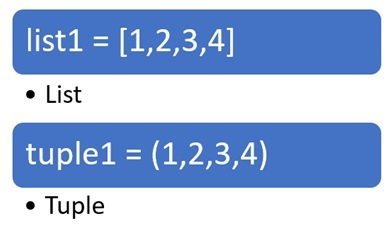
\includegraphics[width=0.5\textwidth]{figures/Difference-Between-List-and-Tuple-fig-1-2.jpg}
\caption{At first glance list and tuples look very similar, but they are not\ldots{}}
\end{figure}

Like lists, tuples are containers of any type of object. Unlike lists though they are \emph{immutable} which means that once they have been created the content cannot be changed (i.e.~no append, insert or delete of the elements). Furthermore since they are immutable they can be used as dictionary keys (lists cannot).
To create a tuple the comma-separated list of items has to be enclosed in brackets, or the $\tt{tuple()}$ operator can be used.
Accessing tuple items is done in exactly the same way as lists.

\begin{tcolorbox}[breakable, size=fbox, boxrule=1pt, pad at break*=1mm, colback=cellbackground, colframe=cellborder]
\begin{Verbatim}[commandchars=\\\{\}]
\PY{n}{atuple} \PY{o}{=} \PY{p}{(}\PY{l+m+mi}{1}\PY{p}{,} \PY{l+m+mi}{2}\PY{p}{,} \PY{l+m+mi}{3}\PY{p}{)}
\PY{n+nb}{print} \PY{p}{(}\PY{l+s+s2}{\PYZdq{}}\PY{l+s+s2}{Length: }\PY{l+s+si}{\PYZob{}\PYZcb{}}\PY{l+s+s2}{\PYZdq{}}\PY{o}{.}\PY{n}{format}\PY{p}{(}\PY{n+nb}{len}\PY{p}{(}\PY{n}{atuple}\PY{p}{)}\PY{p}{)}\PY{p}{)}
\PY{n+nb}{print} \PY{p}{(}\PY{l+s+s2}{\PYZdq{}}\PY{l+s+s2}{First element: }\PY{l+s+si}{\PYZob{}\PYZcb{}}\PY{l+s+s2}{\PYZdq{}}\PY{o}{.}\PY{n}{format}\PY{p}{(}\PY{n}{atuple}\PY{p}{[}\PY{l+m+mi}{0}\PY{p}{]}\PY{p}{)}\PY{p}{)}
\PY{n+nb}{print} \PY{p}{(}\PY{l+s+s2}{\PYZdq{}}\PY{l+s+s2}{Last element: }\PY{l+s+si}{\PYZob{}\PYZcb{}}\PY{l+s+s2}{\PYZdq{}}\PY{o}{.}\PY{n}{format}\PY{p}{(}\PY{n}{atuple}\PY{p}{[}\PY{o}{\PYZhy{}}\PY{l+m+mi}{1}\PY{p}{]}\PY{p}{)}\PY{p}{)}

Length: 3
First element: 1
Last element: 3
\end{Verbatim}
\end{tcolorbox}

In the next snippet of code it is shown the so called unpacking which is another way to assign tuple values to variables.

\begin{tcolorbox}[breakable, size=fbox, boxrule=1pt, pad at break*=1mm, colback=cellbackground, colframe=cellborder]
\begin{Verbatim}[commandchars=\\\{\}]
\PY{n}{x}\PY{p}{,} \PY{n}{y}\PY{p}{,} \PY{n}{z} \PY{o}{=} \PY{p}{(}\PY{l+m+mi}{10}\PY{p}{,} \PY{l+m+mi}{5}\PY{p}{,} \PY{l+m+mi}{12}\PY{p}{)}
\PY{n+nb}{print} \PY{p}{(}\PY{l+s+s2}{\PYZdq{}}\PY{l+s+s2}{coord: x=}\PY{l+s+si}{\PYZob{}\PYZcb{}}\PY{l+s+s2}{ y=}\PY{l+s+si}{\PYZob{}\PYZcb{}}\PY{l+s+s2}{ z=}\PY{l+s+si}{\PYZob{}\PYZcb{}}\PY{l+s+s2}{\PYZdq{}}\PY{o}{.}\PY{n}{format}\PY{p}{(}\PY{n}{x}\PY{p}{,} \PY{n}{y}\PY{p}{,} \PY{n}{z}\PY{p}{)}\PY{p}{)}

coord: x=10 y=5 z=12
\end{Verbatim}
\end{tcolorbox}

If an ntuple has just one element don't forget the comma at the end otherwise it will be treated as a single number.

\begin{tcolorbox}[breakable, size=fbox, boxrule=1pt, pad at break*=1mm, colback=cellbackground, colframe=cellborder]
\begin{Verbatim}[commandchars=\\\{\}]
\PY{n}{tuple2} \PY{o}{=} \PY{p}{(}\PY{l+m+mi}{1}\PY{p}{,}\PY{p}{)}
\PY{n+nb}{print}\PY{p}{(}\PY{n+nb}{type}\PY{p}{(}\PY{n}{tuple2}\PY{p}{)}\PY{p}{)}
\PY{n}{tuple2} \PY{o}{=} \PY{p}{(}\PY{l+m+mi}{1}\PY{p}{)}
\PY{n+nb}{print}\PY{p}{(}\PY{n+nb}{type}\PY{p}{(}\PY{n}{tuple2}\PY{p}{)}\PY{p}{)}

<class 'tuple'>
<class 'int'>
\end{Verbatim}
\end{tcolorbox}

Since a tuple is immutable to add new elements it is necessary to create a new object:

\begin{tcolorbox}[breakable, size=fbox, boxrule=1pt, pad at break*=1mm, colback=cellbackground, colframe=cellborder]\begin{Verbatim}[commandchars=\\\{\}]
\PY{n}{tuple1} \PY{o}{=} \PY{p}{(}\PY{l+m+mi}{1}\PY{p}{,} \PY{l+m+mi}{2}\PY{p}{,} \PY{l+m+mi}{3}\PY{p}{)}
\PY{n}{tuple2} \PY{o}{=} \PY{n}{tuple1} \PY{o}{+} \PY{p}{(}\PY{l+m+mi}{4}\PY{p}{,} \PY{l+m+mi}{5}\PY{p}{)}
\PY{n+nb}{print}\PY{p}{(}\PY{n}{tuple2}\PY{p}{)}

(1,2,3,4,5)
\end{Verbatim}
\end{tcolorbox}

Finally, as already said tuples can be used as dictionary keys:

\begin{tcolorbox}[breakable, size=fbox, boxrule=1pt, pad at break*=1mm, colback=cellbackground, colframe=cellborder]\begin{Verbatim}[commandchars=\\\{\}]
\PY{n}{d} \PY{o}{=} \PY{p}{\PYZob{}}
   \PY{p}{(}\PY{l+s+s1}{\PYZsq{}}\PY{l+s+s1}{Finance}\PY{l+s+s1}{\PYZsq{}}\PY{p}{,} \PY{l+m+mi}{1}\PY{p}{)}\PY{p}{:} \PY{l+s+s1}{\PYZsq{}}\PY{l+s+s1}{Room 8}\PY{l+s+s1}{\PYZsq{}}\PY{p}{,}
    \PY{p}{(}\PY{l+s+s1}{\PYZsq{}}\PY{l+s+s1}{Finance}\PY{l+s+s1}{\PYZsq{}}\PY{p}{,} \PY{l+m+mi}{2}\PY{p}{)}\PY{p}{:} \PY{l+s+s1}{\PYZsq{}}\PY{l+s+s1}{Room 3}\PY{l+s+s1}{\PYZsq{}}\PY{p}{,}
    \PY{p}{(}\PY{l+s+s1}{\PYZsq{}}\PY{l+s+s1}{Math}\PY{l+s+s1}{\PYZsq{}}\PY{p}{,} \PY{l+m+mi}{1}\PY{p}{)}\PY{p}{:} \PY{l+s+s1}{\PYZsq{}}\PY{l+s+s1}{Room 6}\PY{l+s+s1}{\PYZsq{}}\PY{p}{,}
    \PY{p}{(}\PY{l+s+s1}{\PYZsq{}}\PY{l+s+s1}{Programming}\PY{l+s+s1}{\PYZsq{}}\PY{p}{,} \PY{l+m+mi}{1}\PY{p}{)}\PY{p}{:} \PY{l+s+s1}{\PYZsq{}}\PY{l+s+s1}{IT room}\PY{l+s+s1}{\PYZsq{}}
    \PY{p}{\PYZcb{}}
\end{Verbatim}
\end{tcolorbox}

Below the full list of tuple functions:
\begin{tcolorbox}[breakable, size=fbox, boxrule=1pt, pad at break*=1mm,colback=cellbackground, colframe=cellborder]
\begin{Verbatim}[commandchars=\\\{\}]
\PY{n+nb}{dir}\PY{p}{(}\PY{n+nb}{dict}\PY{p}{)}

[...
 'count',
 'index']
\end{Verbatim}
\end{tcolorbox}

%\begin{thebibliography}{9}
%  %\bibitem{survey2019} StackOverflow \emph{The TEXbook}, Addison-Wesley, Reading,Massachusetts, second edition, 1984,
%\bibitem{survey2019} \emph{https://insights.stackoverflow.com/survey/2019}, Stack Overflow, 2019 [Online]
%\bibitem{python_versions} \emph{https://www.python.org/downloads/}, \texttt{python.org} [Online]
%\bibitem{learn_python} \emph{https://www.learnpython.org/it/}, \texttt{learnpython.org} [Online]
%\bibitem{freecamp} \emph{https://www.youtube.com/watch?v=8DvywoWv6fI}, \textt{freeCodeCamp.org} [Online]
%\bibitem{modules} \emph{https://docs.python.org/3/py-modindex.html}, Complete list of \texttt{python} modules [Online]
%\end{thebibliography}
%

\clearpage

% Default to the notebook output style

    


% Inherit from the specified cell style.




    
\documentclass[11pt]{article}

    
    
    \usepackage[T1]{fontenc}
    % Nicer default font (+ math font) than Computer Modern for most use cases
    \usepackage{mathpazo}

    % Basic figure setup, for now with no caption control since it's done
    % automatically by Pandoc (which extracts ![](path) syntax from Markdown).
    \usepackage{graphicx}
    % We will generate all images so they have a width \maxwidth. This means
    % that they will get their normal width if they fit onto the page, but
    % are scaled down if they would overflow the margins.
    \makeatletter
    \def\maxwidth{\ifdim\Gin@nat@width>\linewidth\linewidth
    \else\Gin@nat@width\fi}
    \makeatother
    \let\Oldincludegraphics\includegraphics
    % Set max figure width to be 80% of text width, for now hardcoded.
    \renewcommand{\includegraphics}[1]{\Oldincludegraphics[width=.8\maxwidth]{#1}}
    % Ensure that by default, figures have no caption (until we provide a
    % proper Figure object with a Caption API and a way to capture that
    % in the conversion process - todo).
    \usepackage{caption}
    \DeclareCaptionLabelFormat{nolabel}{}
    \captionsetup{labelformat=nolabel}

    \usepackage{adjustbox} % Used to constrain images to a maximum size 
    \usepackage{xcolor} % Allow colors to be defined
    \usepackage{enumerate} % Needed for markdown enumerations to work
    \usepackage{geometry} % Used to adjust the document margins
    \usepackage{amsmath} % Equations
    \usepackage{amssymb} % Equations
    \usepackage{textcomp} % defines textquotesingle
    % Hack from http://tex.stackexchange.com/a/47451/13684:
    \AtBeginDocument{%
        \def\PYZsq{\textquotesingle}% Upright quotes in Pygmentized code
    }
    \usepackage{upquote} % Upright quotes for verbatim code
    \usepackage{eurosym} % defines \euro
    \usepackage[mathletters]{ucs} % Extended unicode (utf-8) support
    \usepackage[utf8x]{inputenc} % Allow utf-8 characters in the tex document
    \usepackage{fancyvrb} % verbatim replacement that allows latex
    \usepackage{grffile} % extends the file name processing of package graphics 
                         % to support a larger range 
    % The hyperref package gives us a pdf with properly built
    % internal navigation ('pdf bookmarks' for the table of contents,
    % internal cross-reference links, web links for URLs, etc.)
    \usepackage{hyperref}
    \usepackage{longtable} % longtable support required by pandoc >1.10
    \usepackage{booktabs}  % table support for pandoc > 1.12.2
    \usepackage[inline]{enumitem} % IRkernel/repr support (it uses the enumerate* environment)
    \usepackage[normalem]{ulem} % ulem is needed to support strikethroughs (\sout)
                                % normalem makes italics be italics, not underlines
    \usepackage{mathrsfs}
    

    
    
    % Colors for the hyperref package
    \definecolor{urlcolor}{rgb}{0,.145,.698}
    \definecolor{linkcolor}{rgb}{.71,0.21,0.01}
    \definecolor{citecolor}{rgb}{.12,.54,.11}

    % ANSI colors
    \definecolor{ansi-black}{HTML}{3E424D}
    \definecolor{ansi-black-intense}{HTML}{282C36}
    \definecolor{ansi-red}{HTML}{E75C58}
    \definecolor{ansi-red-intense}{HTML}{B22B31}
    \definecolor{ansi-green}{HTML}{00A250}
    \definecolor{ansi-green-intense}{HTML}{007427}
    \definecolor{ansi-yellow}{HTML}{DDB62B}
    \definecolor{ansi-yellow-intense}{HTML}{B27D12}
    \definecolor{ansi-blue}{HTML}{208FFB}
    \definecolor{ansi-blue-intense}{HTML}{0065CA}
    \definecolor{ansi-magenta}{HTML}{D160C4}
    \definecolor{ansi-magenta-intense}{HTML}{A03196}
    \definecolor{ansi-cyan}{HTML}{60C6C8}
    \definecolor{ansi-cyan-intense}{HTML}{258F8F}
    \definecolor{ansi-white}{HTML}{C5C1B4}
    \definecolor{ansi-white-intense}{HTML}{A1A6B2}
    \definecolor{ansi-default-inverse-fg}{HTML}{FFFFFF}
    \definecolor{ansi-default-inverse-bg}{HTML}{000000}

    % commands and environments needed by pandoc snippets
    % extracted from the output of `pandoc -s`
    \providecommand{\tightlist}{%
      \setlength{\itemsep}{0pt}\setlength{\parskip}{0pt}}
    \DefineVerbatimEnvironment{Highlighting}{Verbatim}{commandchars=\\\{\}}
    % Add ',fontsize=\small' for more characters per line
    \newenvironment{Shaded}{}{}
    \newcommand{\KeywordTok}[1]{\textcolor[rgb]{0.00,0.44,0.13}{\textbf{{#1}}}}
    \newcommand{\DataTypeTok}[1]{\textcolor[rgb]{0.56,0.13,0.00}{{#1}}}
    \newcommand{\DecValTok}[1]{\textcolor[rgb]{0.25,0.63,0.44}{{#1}}}
    \newcommand{\BaseNTok}[1]{\textcolor[rgb]{0.25,0.63,0.44}{{#1}}}
    \newcommand{\FloatTok}[1]{\textcolor[rgb]{0.25,0.63,0.44}{{#1}}}
    \newcommand{\CharTok}[1]{\textcolor[rgb]{0.25,0.44,0.63}{{#1}}}
    \newcommand{\StringTok}[1]{\textcolor[rgb]{0.25,0.44,0.63}{{#1}}}
    \newcommand{\CommentTok}[1]{\textcolor[rgb]{0.38,0.63,0.69}{\textit{{#1}}}}
    \newcommand{\OtherTok}[1]{\textcolor[rgb]{0.00,0.44,0.13}{{#1}}}
    \newcommand{\AlertTok}[1]{\textcolor[rgb]{1.00,0.00,0.00}{\textbf{{#1}}}}
    \newcommand{\FunctionTok}[1]{\textcolor[rgb]{0.02,0.16,0.49}{{#1}}}
    \newcommand{\RegionMarkerTok}[1]{{#1}}
    \newcommand{\ErrorTok}[1]{\textcolor[rgb]{1.00,0.00,0.00}{\textbf{{#1}}}}
    \newcommand{\NormalTok}[1]{{#1}}
    
    % Additional commands for more recent versions of Pandoc
    \newcommand{\ConstantTok}[1]{\textcolor[rgb]{0.53,0.00,0.00}{{#1}}}
    \newcommand{\SpecialCharTok}[1]{\textcolor[rgb]{0.25,0.44,0.63}{{#1}}}
    \newcommand{\VerbatimStringTok}[1]{\textcolor[rgb]{0.25,0.44,0.63}{{#1}}}
    \newcommand{\SpecialStringTok}[1]{\textcolor[rgb]{0.73,0.40,0.53}{{#1}}}
    \newcommand{\ImportTok}[1]{{#1}}
    \newcommand{\DocumentationTok}[1]{\textcolor[rgb]{0.73,0.13,0.13}{\textit{{#1}}}}
    \newcommand{\AnnotationTok}[1]{\textcolor[rgb]{0.38,0.63,0.69}{\textbf{\textit{{#1}}}}}
    \newcommand{\CommentVarTok}[1]{\textcolor[rgb]{0.38,0.63,0.69}{\textbf{\textit{{#1}}}}}
    \newcommand{\VariableTok}[1]{\textcolor[rgb]{0.10,0.09,0.49}{{#1}}}
    \newcommand{\ControlFlowTok}[1]{\textcolor[rgb]{0.00,0.44,0.13}{\textbf{{#1}}}}
    \newcommand{\OperatorTok}[1]{\textcolor[rgb]{0.40,0.40,0.40}{{#1}}}
    \newcommand{\BuiltInTok}[1]{{#1}}
    \newcommand{\ExtensionTok}[1]{{#1}}
    \newcommand{\PreprocessorTok}[1]{\textcolor[rgb]{0.74,0.48,0.00}{{#1}}}
    \newcommand{\AttributeTok}[1]{\textcolor[rgb]{0.49,0.56,0.16}{{#1}}}
    \newcommand{\InformationTok}[1]{\textcolor[rgb]{0.38,0.63,0.69}{\textbf{\textit{{#1}}}}}
    \newcommand{\WarningTok}[1]{\textcolor[rgb]{0.38,0.63,0.69}{\textbf{\textit{{#1}}}}}
    
    
    % Define a nice break command that doesn't care if a line doesn't already
    % exist.
    \def\br{\hspace*{\fill} \\* }
    % Math Jax compatibility definitions
    \def\gt{>}
    \def\lt{<}
    \let\Oldtex\TeX
    \let\Oldlatex\LaTeX
    \renewcommand{\TeX}{\textrm{\Oldtex}}
    \renewcommand{\LaTeX}{\textrm{\Oldlatex}}
    % Document parameters
    % Document title
    \title{Interpolation - Practical Lesson 3}
    \author {Matteo Sani \\ \href{mailto:matteosan1@gmail.com}{matteosan1@gmail.com}}
    
    
    
    

    % Pygments definitions
    
\makeatletter
\def\PY@reset{\let\PY@it=\relax \let\PY@bf=\relax%
    \let\PY@ul=\relax \let\PY@tc=\relax%
    \let\PY@bc=\relax \let\PY@ff=\relax}
\def\PY@tok#1{\csname PY@tok@#1\endcsname}
\def\PY@toks#1+{\ifx\relax#1\empty\else%
    \PY@tok{#1}\expandafter\PY@toks\fi}
\def\PY@do#1{\PY@bc{\PY@tc{\PY@ul{%
    \PY@it{\PY@bf{\PY@ff{#1}}}}}}}
\def\PY#1#2{\PY@reset\PY@toks#1+\relax+\PY@do{#2}}

\expandafter\def\csname PY@tok@w\endcsname{\def\PY@tc##1{\textcolor[rgb]{0.73,0.73,0.73}{##1}}}
\expandafter\def\csname PY@tok@c\endcsname{\let\PY@it=\textit\def\PY@tc##1{\textcolor[rgb]{0.25,0.50,0.50}{##1}}}
\expandafter\def\csname PY@tok@cp\endcsname{\def\PY@tc##1{\textcolor[rgb]{0.74,0.48,0.00}{##1}}}
\expandafter\def\csname PY@tok@k\endcsname{\let\PY@bf=\textbf\def\PY@tc##1{\textcolor[rgb]{0.00,0.50,0.00}{##1}}}
\expandafter\def\csname PY@tok@kp\endcsname{\def\PY@tc##1{\textcolor[rgb]{0.00,0.50,0.00}{##1}}}
\expandafter\def\csname PY@tok@kt\endcsname{\def\PY@tc##1{\textcolor[rgb]{0.69,0.00,0.25}{##1}}}
\expandafter\def\csname PY@tok@o\endcsname{\def\PY@tc##1{\textcolor[rgb]{0.40,0.40,0.40}{##1}}}
\expandafter\def\csname PY@tok@ow\endcsname{\let\PY@bf=\textbf\def\PY@tc##1{\textcolor[rgb]{0.67,0.13,1.00}{##1}}}
\expandafter\def\csname PY@tok@nb\endcsname{\def\PY@tc##1{\textcolor[rgb]{0.00,0.50,0.00}{##1}}}
\expandafter\def\csname PY@tok@nf\endcsname{\def\PY@tc##1{\textcolor[rgb]{0.00,0.00,1.00}{##1}}}
\expandafter\def\csname PY@tok@nc\endcsname{\let\PY@bf=\textbf\def\PY@tc##1{\textcolor[rgb]{0.00,0.00,1.00}{##1}}}
\expandafter\def\csname PY@tok@nn\endcsname{\let\PY@bf=\textbf\def\PY@tc##1{\textcolor[rgb]{0.00,0.00,1.00}{##1}}}
\expandafter\def\csname PY@tok@ne\endcsname{\let\PY@bf=\textbf\def\PY@tc##1{\textcolor[rgb]{0.82,0.25,0.23}{##1}}}
\expandafter\def\csname PY@tok@nv\endcsname{\def\PY@tc##1{\textcolor[rgb]{0.10,0.09,0.49}{##1}}}
\expandafter\def\csname PY@tok@no\endcsname{\def\PY@tc##1{\textcolor[rgb]{0.53,0.00,0.00}{##1}}}
\expandafter\def\csname PY@tok@nl\endcsname{\def\PY@tc##1{\textcolor[rgb]{0.63,0.63,0.00}{##1}}}
\expandafter\def\csname PY@tok@ni\endcsname{\let\PY@bf=\textbf\def\PY@tc##1{\textcolor[rgb]{0.60,0.60,0.60}{##1}}}
\expandafter\def\csname PY@tok@na\endcsname{\def\PY@tc##1{\textcolor[rgb]{0.49,0.56,0.16}{##1}}}
\expandafter\def\csname PY@tok@nt\endcsname{\let\PY@bf=\textbf\def\PY@tc##1{\textcolor[rgb]{0.00,0.50,0.00}{##1}}}
\expandafter\def\csname PY@tok@nd\endcsname{\def\PY@tc##1{\textcolor[rgb]{0.67,0.13,1.00}{##1}}}
\expandafter\def\csname PY@tok@s\endcsname{\def\PY@tc##1{\textcolor[rgb]{0.73,0.13,0.13}{##1}}}
\expandafter\def\csname PY@tok@sd\endcsname{\let\PY@it=\textit\def\PY@tc##1{\textcolor[rgb]{0.73,0.13,0.13}{##1}}}
\expandafter\def\csname PY@tok@si\endcsname{\let\PY@bf=\textbf\def\PY@tc##1{\textcolor[rgb]{0.73,0.40,0.53}{##1}}}
\expandafter\def\csname PY@tok@se\endcsname{\let\PY@bf=\textbf\def\PY@tc##1{\textcolor[rgb]{0.73,0.40,0.13}{##1}}}
\expandafter\def\csname PY@tok@sr\endcsname{\def\PY@tc##1{\textcolor[rgb]{0.73,0.40,0.53}{##1}}}
\expandafter\def\csname PY@tok@ss\endcsname{\def\PY@tc##1{\textcolor[rgb]{0.10,0.09,0.49}{##1}}}
\expandafter\def\csname PY@tok@sx\endcsname{\def\PY@tc##1{\textcolor[rgb]{0.00,0.50,0.00}{##1}}}
\expandafter\def\csname PY@tok@m\endcsname{\def\PY@tc##1{\textcolor[rgb]{0.40,0.40,0.40}{##1}}}
\expandafter\def\csname PY@tok@gh\endcsname{\let\PY@bf=\textbf\def\PY@tc##1{\textcolor[rgb]{0.00,0.00,0.50}{##1}}}
\expandafter\def\csname PY@tok@gu\endcsname{\let\PY@bf=\textbf\def\PY@tc##1{\textcolor[rgb]{0.50,0.00,0.50}{##1}}}
\expandafter\def\csname PY@tok@gd\endcsname{\def\PY@tc##1{\textcolor[rgb]{0.63,0.00,0.00}{##1}}}
\expandafter\def\csname PY@tok@gi\endcsname{\def\PY@tc##1{\textcolor[rgb]{0.00,0.63,0.00}{##1}}}
\expandafter\def\csname PY@tok@gr\endcsname{\def\PY@tc##1{\textcolor[rgb]{1.00,0.00,0.00}{##1}}}
\expandafter\def\csname PY@tok@ge\endcsname{\let\PY@it=\textit}
\expandafter\def\csname PY@tok@gs\endcsname{\let\PY@bf=\textbf}
\expandafter\def\csname PY@tok@gp\endcsname{\let\PY@bf=\textbf\def\PY@tc##1{\textcolor[rgb]{0.00,0.00,0.50}{##1}}}
\expandafter\def\csname PY@tok@go\endcsname{\def\PY@tc##1{\textcolor[rgb]{0.53,0.53,0.53}{##1}}}
\expandafter\def\csname PY@tok@gt\endcsname{\def\PY@tc##1{\textcolor[rgb]{0.00,0.27,0.87}{##1}}}
\expandafter\def\csname PY@tok@err\endcsname{\def\PY@bc##1{\setlength{\fboxsep}{0pt}\fcolorbox[rgb]{1.00,0.00,0.00}{1,1,1}{\strut ##1}}}
\expandafter\def\csname PY@tok@kc\endcsname{\let\PY@bf=\textbf\def\PY@tc##1{\textcolor[rgb]{0.00,0.50,0.00}{##1}}}
\expandafter\def\csname PY@tok@kd\endcsname{\let\PY@bf=\textbf\def\PY@tc##1{\textcolor[rgb]{0.00,0.50,0.00}{##1}}}
\expandafter\def\csname PY@tok@kn\endcsname{\let\PY@bf=\textbf\def\PY@tc##1{\textcolor[rgb]{0.00,0.50,0.00}{##1}}}
\expandafter\def\csname PY@tok@kr\endcsname{\let\PY@bf=\textbf\def\PY@tc##1{\textcolor[rgb]{0.00,0.50,0.00}{##1}}}
\expandafter\def\csname PY@tok@bp\endcsname{\def\PY@tc##1{\textcolor[rgb]{0.00,0.50,0.00}{##1}}}
\expandafter\def\csname PY@tok@fm\endcsname{\def\PY@tc##1{\textcolor[rgb]{0.00,0.00,1.00}{##1}}}
\expandafter\def\csname PY@tok@vc\endcsname{\def\PY@tc##1{\textcolor[rgb]{0.10,0.09,0.49}{##1}}}
\expandafter\def\csname PY@tok@vg\endcsname{\def\PY@tc##1{\textcolor[rgb]{0.10,0.09,0.49}{##1}}}
\expandafter\def\csname PY@tok@vi\endcsname{\def\PY@tc##1{\textcolor[rgb]{0.10,0.09,0.49}{##1}}}
\expandafter\def\csname PY@tok@vm\endcsname{\def\PY@tc##1{\textcolor[rgb]{0.10,0.09,0.49}{##1}}}
\expandafter\def\csname PY@tok@sa\endcsname{\def\PY@tc##1{\textcolor[rgb]{0.73,0.13,0.13}{##1}}}
\expandafter\def\csname PY@tok@sb\endcsname{\def\PY@tc##1{\textcolor[rgb]{0.73,0.13,0.13}{##1}}}
\expandafter\def\csname PY@tok@sc\endcsname{\def\PY@tc##1{\textcolor[rgb]{0.73,0.13,0.13}{##1}}}
\expandafter\def\csname PY@tok@dl\endcsname{\def\PY@tc##1{\textcolor[rgb]{0.73,0.13,0.13}{##1}}}
\expandafter\def\csname PY@tok@s2\endcsname{\def\PY@tc##1{\textcolor[rgb]{0.73,0.13,0.13}{##1}}}
\expandafter\def\csname PY@tok@sh\endcsname{\def\PY@tc##1{\textcolor[rgb]{0.73,0.13,0.13}{##1}}}
\expandafter\def\csname PY@tok@s1\endcsname{\def\PY@tc##1{\textcolor[rgb]{0.73,0.13,0.13}{##1}}}
\expandafter\def\csname PY@tok@mb\endcsname{\def\PY@tc##1{\textcolor[rgb]{0.40,0.40,0.40}{##1}}}
\expandafter\def\csname PY@tok@mf\endcsname{\def\PY@tc##1{\textcolor[rgb]{0.40,0.40,0.40}{##1}}}
\expandafter\def\csname PY@tok@mh\endcsname{\def\PY@tc##1{\textcolor[rgb]{0.40,0.40,0.40}{##1}}}
\expandafter\def\csname PY@tok@mi\endcsname{\def\PY@tc##1{\textcolor[rgb]{0.40,0.40,0.40}{##1}}}
\expandafter\def\csname PY@tok@il\endcsname{\def\PY@tc##1{\textcolor[rgb]{0.40,0.40,0.40}{##1}}}
\expandafter\def\csname PY@tok@mo\endcsname{\def\PY@tc##1{\textcolor[rgb]{0.40,0.40,0.40}{##1}}}
\expandafter\def\csname PY@tok@ch\endcsname{\let\PY@it=\textit\def\PY@tc##1{\textcolor[rgb]{0.25,0.50,0.50}{##1}}}
\expandafter\def\csname PY@tok@cm\endcsname{\let\PY@it=\textit\def\PY@tc##1{\textcolor[rgb]{0.25,0.50,0.50}{##1}}}
\expandafter\def\csname PY@tok@cpf\endcsname{\let\PY@it=\textit\def\PY@tc##1{\textcolor[rgb]{0.25,0.50,0.50}{##1}}}
\expandafter\def\csname PY@tok@c1\endcsname{\let\PY@it=\textit\def\PY@tc##1{\textcolor[rgb]{0.25,0.50,0.50}{##1}}}
\expandafter\def\csname PY@tok@cs\endcsname{\let\PY@it=\textit\def\PY@tc##1{\textcolor[rgb]{0.25,0.50,0.50}{##1}}}

\def\PYZbs{\char`\\}
\def\PYZus{\char`\_}
\def\PYZob{\char`\{}
\def\PYZcb{\char`\}}
\def\PYZca{\char`\^}
\def\PYZam{\char`\&}
\def\PYZlt{\char`\<}
\def\PYZgt{\char`\>}
\def\PYZsh{\char`\#}
\def\PYZpc{\char`\%}
\def\PYZdl{\char`\$}
\def\PYZhy{\char`\-}
\def\PYZsq{\char`\'}
\def\PYZdq{\char`\"}
\def\PYZti{\char`\~}
% for compatibility with earlier versions
\def\PYZat{@}
\def\PYZlb{[}
\def\PYZrb{]}
\makeatother


    % Exact colors from NB
    \definecolor{incolor}{rgb}{0.0, 0.0, 0.5}
    \definecolor{outcolor}{rgb}{0.545, 0.0, 0.0}



    
    % Prevent overflowing lines due to hard-to-break entities
    \sloppy 
    % Setup hyperref package
    \hypersetup{
      breaklinks=true,  % so long urls are correctly broken across lines
      colorlinks=true,
      urlcolor=urlcolor,
      linkcolor=linkcolor,
      citecolor=citecolor,
      }
    % Slightly bigger margins than the latex defaults
    
    \geometry{verbose,tmargin=1in,bmargin=1in,lmargin=1in,rmargin=1in}
    
    

    \begin{document}
    
    
    \maketitle
    
    

    
    \hypertarget{interpolation---practical-lesson-3}{%
\section{Interpolation}\label{interpolation---practical-lesson-3}}

\hypertarget{recap}{%
\subsection{Recap}\label{recap}}

Last lesson we looked at:

\begin{itemize}
\tightlist
\item
  \texttt{print} statements and variables
\item
  mathematical expressions, also importing functions from a module
  (specifically the log and exp functions from the math module)
\item
  boolean expressions
\item
  string expressions
\item
  indentation, \texttt{if/elif/else} blocks and \texttt{for} loops
\item
  lists
\item
  dictionaries
\item
  tuples
\item
  dates
\item
  functions and modules
\end{itemize}

    \hypertarget{exercise-interpolation-extrapolation}{%
\subsection{Exercise Interpolation /
Extrapolation}\label{exercise-interpolation-extrapolation}}

\hypertarget{linear-interpolation}{%
\subsubsection{Linear interpolation}\label{linear-interpolation}}

Interpolation is a method of constructing new data points within the
range of a discrete set of known data points.

It may happen to have few data points, obtained by sampling or
experimenting, which represent the values of a function for a limited
number of values of an independent variable (e.g.~in recording a trip:
distances at certain times). It is often required to interpolate,
i.e.~estimate the value of that function for an intermediate value of
the independent variable (e.g.~in our previous example what is the
distance at new times ?).

Let's exercise on linear interpolation (and extrapolation because yes in
same cases you can also get new points outside the measured range) with
a couple of examples.

\hypertarget{example-1}{%
\paragraph{Example 1}\label{example-1}}

Assume you are going on holidays by car and that luckily there isn't
much traffic so that you can drive at constant speed (which gives a
linear relation between travelled space and time i.e. \(s = v \cdot t\),
which means that if you'd plot the distances \(s\) as a function of the
time \(t\) you get a line with slope \(v\)). Given two samples of the
car travelled distance \(s_1\) and \(s_2\) taken at two different times
\(t_1\) and \(t_2\) you can linearly interpolate to find your position
at different times using the following relations:

\begin{equation}
w = \frac{t - t_1}{t_2 - t_1}
\end{equation}
$t$ generic time at which we want to know the distance $s$,
\begin{equation}
s = (1 - w)\cdot s\_1 + w \cdot s\_2
\end{equation}


\textbf{\emph{Derivation}}
The equation of a line for two points
\((t_1, s_1)\) and \((t_2, s_2)\) can be written as:
\begin{equation}
\frac{t - t_1}{t_2 - t_1} = \frac{s - s_1}{s_2 - s_1}
\end{equation}

Setting $ w = \frac{t - t_1}{t_2 - t_1}$ and solving for $s$ we find
the desired solution:
\begin{equation}
  w = \frac{s - s_1}{s_2 - s_1} \Rightarrow (s_2 - s_1)\cdot w = s - s_1 \Rightarrow ...
\end{equation}

Back to our example, if
\(s_1 = 25.75~\mathrm{km}\;(@t_1 = 15~\mathrm{min})\) and
\(s_2 = 171.7~\mathrm{km}\;(@t_2 = 100~\mathrm{min})\) let's compute:

    \begin{Verbatim}[commandchars=\\\{\}]
{\color{incolor}In [{\color{incolor}1}]:} \PY{c+c1}{\PYZsh{} let\PYZsq{}s find distance travelled in 1 hour (interpolation)}
        
        \PY{n}{s\PYZus{}1} \PY{o}{=} \PY{l+m+mf}{25.75} \PY{c+c1}{\PYZsh{} distance in km}
        \PY{n}{t\PYZus{}1} \PY{o}{=} \PY{l+m+mi}{15}    \PY{c+c1}{\PYZsh{} elapsed time in minutes}
        \PY{n}{s\PYZus{}2} \PY{o}{=} \PY{l+m+mf}{171.7}
        \PY{n}{t\PYZus{}2} \PY{o}{=} \PY{l+m+mi}{100}
        
        \PY{n}{t} \PY{o}{=} \PY{l+m+mi}{60}
        
        \PY{n}{w} \PY{o}{=} \PY{p}{(}\PY{n}{t} \PY{o}{\PYZhy{}} \PY{n}{t\PYZus{}1}\PY{p}{)}\PY{o}{/}\PY{p}{(}\PY{n}{t\PYZus{}2} \PY{o}{\PYZhy{}} \PY{n}{t\PYZus{}1}\PY{p}{)}
        \PY{n}{s} \PY{o}{=} \PY{p}{(}\PY{l+m+mi}{1} \PY{o}{\PYZhy{}} \PY{n}{w}\PY{p}{)}\PY{o}{*}\PY{n}{s\PYZus{}1} \PY{o}{+} \PY{n}{w}\PY{o}{*}\PY{n}{s\PYZus{}2}
        
        \PY{n+nb}{print} \PY{p}{(}\PY{l+s+s2}{\PYZdq{}}\PY{l+s+si}{\PYZob{}:.1f\PYZcb{}}\PY{l+s+s2}{ km}\PY{l+s+s2}{\PYZdq{}}\PY{o}{.}\PY{n}{format}\PY{p}{(}\PY{n}{s}\PY{p}{)}\PY{p}{)}
\end{Verbatim}

    \begin{Verbatim}[commandchars=\\\{\}]
103.0 km

    \end{Verbatim}

    \begin{Verbatim}[commandchars=\\\{\}]
{\color{incolor}In [{\color{incolor}2}]:} \PY{c+c1}{\PYZsh{} distance travelled in first 10 minutes }
        \PY{c+c1}{\PYZsh{} (extrapolation because we are outside of the measured points)}
        
        \PY{n}{s\PYZus{}1} \PY{o}{=} \PY{l+m+mf}{25.75} \PY{c+c1}{\PYZsh{} distance in km}
        \PY{n}{t\PYZus{}1} \PY{o}{=} \PY{l+m+mi}{15}    \PY{c+c1}{\PYZsh{} elapsed time in minutes}
        \PY{n}{s\PYZus{}2} \PY{o}{=} \PY{l+m+mf}{171.7}
        \PY{n}{t\PYZus{}2} \PY{o}{=} \PY{l+m+mi}{100}
        
        \PY{n}{t} \PY{o}{=} \PY{l+m+mi}{10}
        
        \PY{n}{w} \PY{o}{=} \PY{p}{(}\PY{n}{t} \PY{o}{\PYZhy{}} \PY{n}{t\PYZus{}1}\PY{p}{)}\PY{o}{/}\PY{p}{(}\PY{n}{t\PYZus{}2} \PY{o}{\PYZhy{}} \PY{n}{t\PYZus{}1}\PY{p}{)}
        \PY{n}{s} \PY{o}{=} \PY{p}{(}\PY{l+m+mi}{1} \PY{o}{\PYZhy{}} \PY{n}{w}\PY{p}{)}\PY{o}{*}\PY{n}{s\PYZus{}1} \PY{o}{+} \PY{n}{w}\PY{o}{*}\PY{n}{s\PYZus{}2}
        
        \PY{n+nb}{print} \PY{p}{(}\PY{l+s+s2}{\PYZdq{}}\PY{l+s+si}{\PYZob{}:.1f\PYZcb{}}\PY{l+s+s2}{ km}\PY{l+s+s2}{\PYZdq{}}\PY{o}{.}\PY{n}{format}\PY{p}{(}\PY{n}{s}\PY{p}{)}\PY{p}{)}
\end{Verbatim}

    \begin{Verbatim}[commandchars=\\\{\}]
17.2 km

    \end{Verbatim}

    \begin{Verbatim}[commandchars=\\\{\}]
{\color{incolor}In [{\color{incolor}3}]:} \PY{c+c1}{\PYZsh{} distance travelled in a 3 hour trip (extrapolation)}
        
        \PY{n}{s\PYZus{}1} \PY{o}{=} \PY{l+m+mf}{25.75} \PY{c+c1}{\PYZsh{} distance in km}
        \PY{n}{t\PYZus{}1} \PY{o}{=} \PY{l+m+mi}{15}    \PY{c+c1}{\PYZsh{} elapsed time in minutes}
        \PY{n}{s\PYZus{}2} \PY{o}{=} \PY{l+m+mf}{171.7}
        \PY{n}{t\PYZus{}2} \PY{o}{=} \PY{l+m+mi}{100}
        
        \PY{n}{t} \PY{o}{=} \PY{l+m+mi}{180}
        
        \PY{n}{w} \PY{o}{=} \PY{p}{(}\PY{n}{t} \PY{o}{\PYZhy{}} \PY{n}{t\PYZus{}1}\PY{p}{)}\PY{o}{/}\PY{p}{(}\PY{n}{t\PYZus{}2} \PY{o}{\PYZhy{}} \PY{n}{t\PYZus{}1}\PY{p}{)}
        \PY{n}{s} \PY{o}{=} \PY{p}{(}\PY{l+m+mi}{1} \PY{o}{\PYZhy{}} \PY{n}{w}\PY{p}{)}\PY{o}{*}\PY{n}{s\PYZus{}1} \PY{o}{+} \PY{n}{w}\PY{o}{*}\PY{n}{s\PYZus{}2}
        
        \PY{n+nb}{print} \PY{p}{(}\PY{l+s+s2}{\PYZdq{}}\PY{l+s+si}{\PYZob{}:.1f\PYZcb{}}\PY{l+s+s2}{ km}\PY{l+s+s2}{\PYZdq{}}\PY{o}{.}\PY{n}{format}\PY{p}{(}\PY{n}{s}\PY{p}{)}\PY{p}{)}
\end{Verbatim}

    \begin{Verbatim}[commandchars=\\\{\}]
309.1 km

    \end{Verbatim}

    \hypertarget{log-linear-interpolation}{%
\subsubsection{Log-linear
interpolation}\label{log-linear-interpolation}}

When the variable we would like to interpolate has an exponential
relation with the unknown we can fall back to the previous case by
applying the logarithm. In this case the previous formulas apply again
except that at the end we have to exponentiate to get back the original
variable:
\begin{equation}
p = \mathrm{exp}(c \cdot h)
\end{equation}
\begin{equation}
s = \mathrm{log}(p) = \mathrm{log}(\mathrm{exp}(c \cdot h)) = c
\cdot h
\end{equation}
\begin{equation}
w = \frac{h - h_1}{h_2 - h_1}
\end{equation}
\begin{equation}
s = (1 - w)\cdot s\_1 + w \cdot s\_2;;(\mathrm{remember \;now };s =
\mathrm{log}(p))
\end{equation}
\begin{equation}
p = \mathrm{exp}(s)
\end{equation}

Let's see a practical example.

\hypertarget{example-2}{%
\paragraph{Example 2}\label{example-2}}

Atmospheric pressure decreases with the altitude (i.e.~the highest I
flight the lower is the pressure) following an exponential law:
\begin{equation}
p = p_0\cdot e^{-\alpha h}
\end{equation}

where
\begin{itemize}
\item $h$ is the altitude
\item $p_0$ is the pressure at sea level
\item $\alpha$ is a constant
\end{itemize}

Taking the logarithm of each side of the equation I get a linear
relation which can be interpolated as before:
\begin{equation}
  \tilde{s} = \mathrm{log}(p) = \mathrm{log}(p_0\cdot e^{-\alpha h})\propto - \alpha \cdot h
\end{equation}

Now assume that we have measured
\(p_1 = 90~\mathrm{kPa}\;(h_1 = 1000~\mathrm{m})\) and
\(p_2 = 40~\mathrm{kPa}\;(h_1 = 7000~\mathrm{m})\) what will be the
atmospheric pressure on top of the Mont Blanc (\(4812~\mathrm{m}\)) ?
and on top of Mount Everest (\(8848~\mathrm{m}\)) ?

    \begin{Verbatim}[commandchars=\\\{\}]
{\color{incolor}In [{\color{incolor}4}]:} \PY{c+c1}{\PYZsh{} pressure on top of the Mont Blanc (interpolation)}
        \PY{k+kn}{from} \PY{n+nn}{math} \PY{k}{import} \PY{n}{log}\PY{p}{,} \PY{n}{exp}
        
        \PY{c+c1}{\PYZsh{} first we take the logarithm of our measurements to use the linear }
        \PY{c+c1}{\PYZsh{} relation to interpolate}
        \PY{n}{h\PYZus{}1} \PY{o}{=} \PY{l+m+mi}{1000} \PY{c+c1}{\PYZsh{} height in meters}
        \PY{n}{s\PYZus{}1} \PY{o}{=} \PY{n}{log}\PY{p}{(}\PY{l+m+mi}{90}\PY{p}{)} \PY{c+c1}{\PYZsh{} logarithm of the pressure at heigth h1}
        \PY{n}{h\PYZus{}2} \PY{o}{=} \PY{l+m+mi}{7000} \PY{c+c1}{\PYZsh{} height in meters}
        \PY{n}{s\PYZus{}2} \PY{o}{=} \PY{n}{log}\PY{p}{(}\PY{l+m+mi}{40}\PY{p}{)} \PY{c+c1}{\PYZsh{} logarithm of the pressure at heigth h2}
        
        \PY{n}{h} \PY{o}{=} \PY{l+m+mi}{4812}
        
        \PY{n}{w} \PY{o}{=} \PY{p}{(}\PY{n}{h} \PY{o}{\PYZhy{}} \PY{n}{h\PYZus{}1}\PY{p}{)}\PY{o}{/}\PY{p}{(}\PY{n}{h\PYZus{}2} \PY{o}{\PYZhy{}} \PY{n}{h\PYZus{}1}\PY{p}{)}
        \PY{n}{s} \PY{o}{=} \PY{p}{(}\PY{l+m+mi}{1} \PY{o}{\PYZhy{}} \PY{n}{w}\PY{p}{)}\PY{o}{*}\PY{n}{s\PYZus{}1} \PY{o}{+} \PY{n}{w}\PY{o}{*}\PY{n}{s\PYZus{}2}
        
        \PY{n+nb}{print} \PY{p}{(}\PY{l+s+s2}{\PYZdq{}}\PY{l+s+si}{\PYZob{}:.1f\PYZcb{}}\PY{l+s+s2}{ kPa}\PY{l+s+s2}{\PYZdq{}}\PY{o}{.}\PY{n}{format}\PY{p}{(}\PY{n}{exp}\PY{p}{(}\PY{n}{s}\PY{p}{)}\PY{p}{)}\PY{p}{)}
\end{Verbatim}

    \begin{Verbatim}[commandchars=\\\{\}]
53.8 kPa

    \end{Verbatim}

    \begin{Verbatim}[commandchars=\\\{\}]
{\color{incolor}In [{\color{incolor}5}]:} \PY{c+c1}{\PYZsh{} pressure on top of the Mount Everest (extrapolation)}
        \PY{k+kn}{from} \PY{n+nn}{math} \PY{k}{import} \PY{n}{log}\PY{p}{,} \PY{n}{exp}
        
        \PY{c+c1}{\PYZsh{} first we take the logarithm of our measurements to use the linear }
        \PY{c+c1}{\PYZsh{} relation to interpolate}
        \PY{n}{h\PYZus{}1} \PY{o}{=} \PY{l+m+mi}{1000} \PY{c+c1}{\PYZsh{} height in meters}
        \PY{n}{s\PYZus{}1} \PY{o}{=} \PY{n}{log}\PY{p}{(}\PY{l+m+mi}{90}\PY{p}{)} \PY{c+c1}{\PYZsh{} logarithm of the pressure at heigth h1}
        \PY{n}{h\PYZus{}2} \PY{o}{=} \PY{l+m+mi}{7000} \PY{c+c1}{\PYZsh{} height in meters}
        \PY{n}{s\PYZus{}2} \PY{o}{=} \PY{n}{log}\PY{p}{(}\PY{l+m+mi}{40}\PY{p}{)} \PY{c+c1}{\PYZsh{} logarithm of the pressure at heigth h2}
        
        \PY{n}{h} \PY{o}{=} \PY{l+m+mi}{8848}
        
        \PY{n}{w} \PY{o}{=} \PY{p}{(}\PY{n}{h} \PY{o}{\PYZhy{}} \PY{n}{h\PYZus{}1}\PY{p}{)}\PY{o}{/}\PY{p}{(}\PY{n}{h\PYZus{}2} \PY{o}{\PYZhy{}} \PY{n}{h\PYZus{}1}\PY{p}{)}
        \PY{n}{s} \PY{o}{=} \PY{p}{(}\PY{l+m+mi}{1} \PY{o}{\PYZhy{}} \PY{n}{w}\PY{p}{)}\PY{o}{*}\PY{n}{s\PYZus{}1} \PY{o}{+} \PY{n}{w}\PY{o}{*}\PY{n}{s\PYZus{}2}
        
        \PY{n+nb}{print} \PY{p}{(}\PY{l+s+s2}{\PYZdq{}}\PY{l+s+si}{\PYZob{}:.1f\PYZcb{}}\PY{l+s+s2}{ kPa}\PY{l+s+s2}{\PYZdq{}}\PY{o}{.}\PY{n}{format}\PY{p}{(}\PY{n}{exp}\PY{p}{(}\PY{n}{s}\PY{p}{)}\PY{p}{)}\PY{p}{)}
\end{Verbatim}

    \begin{Verbatim}[commandchars=\\\{\}]
31.2 kPa

    \end{Verbatim}

    \begin{figure}
\centering
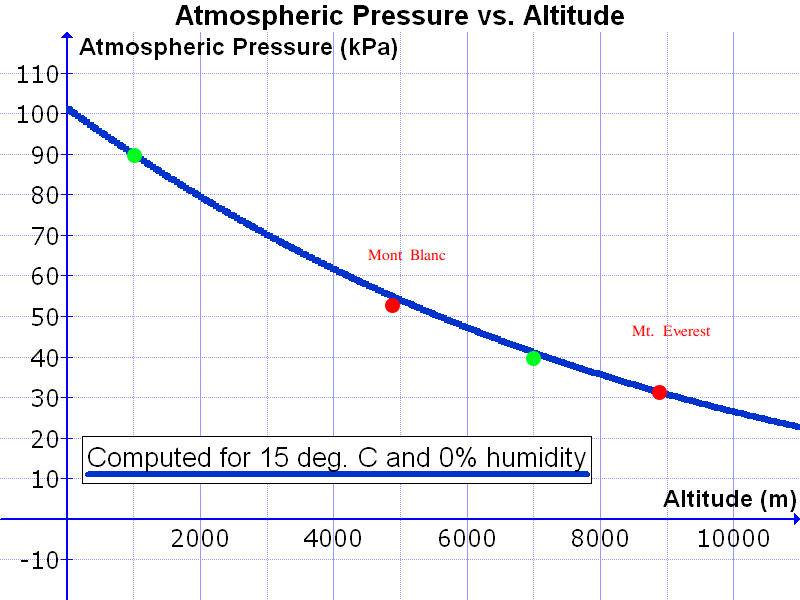
\includegraphics{Atmospheric_Pressure_vs._Altitude.png}
\caption{Atmospheric pressure versus altitude (wikipedia). Green points
represent our measurements, red points represent
interpolation/extrapolation.}
\end{figure}

    \hypertarget{discount-curve-interpolation}{%
\subsection{Discount curve
interpolation}\label{discount-curve-interpolation}}

Now we can come back to finance and using what we have just learnt try
to write a function which interpolates some given discount factors.

Needed data: * a list of pillars dates specifying the value dates of the
given discount factors, \(t_0,...,t_{n-1}\) * a list of given discount
factors, \(D(t_0),...,D(t_{n-1})\) * a pricing date (`today' date) which
corresponds to \(t=0\)

The input argument to the function will be the value date at which we
want to interpolate the discount factor.

Since the discount factor can be expresses as \(D=e^{-r(T-t)}\) the
function will use a log-linear interpolation to return the value we are
looking for.

\[D(t) = \mathrm{exp}\Big( (1-w)\cdot \mathrm{ln}(D(t_i)) + w\cdot \mathrm{ln}(D(t_{i+1}))\Big);\;\;\;w=\frac{t-t_i}{t_{i+1}-t_i}\]

where \(i\) is such that \(t_i \le t \le t_{i+1}\). More technically we
can say that we are doing a linear interpolation over time in the log
space:

\[d(t_i):=\mathrm{ln}(D(t_i))\]

\[d(t) = (1-w)d(t_i) + wd(t_{i+1});\;\;\;w=\frac{t-t_i}{t_{i+1}-t_i}\]

\[D(t) = \mathrm{exp}(d(t))\]

where \(i\) is such that \(t_i \le t \le t_{i+1}\)

Instead of reinventing the wheel and perform the interpolation with our
own code, we'll use the function \texttt{interp} provided by the Python
module \texttt{numpy}. So first let's try it with some simple examples:

    \begin{Verbatim}[commandchars=\\\{\}]
{\color{incolor}In [{\color{incolor}8}]:} \PY{c+c1}{\PYZsh{} let\PYZsq{}s assume we have a list \PYZsq{}xp\PYZsq{} of x-axis coordinates,}
        \PY{c+c1}{\PYZsh{} and the corresponding values \PYZsq{}fp\PYZsq{} of a function evaluated }
        \PY{c+c1}{\PYZsh{} at those x coordinates.}
        \PY{n}{xp} \PY{o}{=} \PY{p}{[}\PY{l+m+mi}{1}\PY{p}{,} \PY{l+m+mi}{2}\PY{p}{,} \PY{l+m+mi}{3}\PY{p}{]}
        \PY{n}{fp} \PY{o}{=} \PY{p}{[}\PY{l+m+mf}{0.3}\PY{p}{,} \PY{l+m+mf}{0.4}\PY{p}{,} \PY{l+m+mf}{0.6}\PY{p}{]}
        
        \PY{c+c1}{\PYZsh{} let\PYZsq{}s see what this looks like when plotted on a graph}
        \PY{c+c1}{\PYZsh{} we briefly introduce here the matplotlib module}
        \PY{c+c1}{\PYZsh{} the keyword as allows to give shorter names to modules}
        \PY{k+kn}{from} \PY{n+nn}{matplotlib} \PY{k}{import} \PY{n}{pyplot} \PY{k}{as} \PY{n}{plt}
        \PY{n}{plt}\PY{o}{.}\PY{n}{plot}\PY{p}{(}\PY{n}{xp}\PY{p}{,} \PY{n}{fp}\PY{p}{,} \PY{n}{marker}\PY{o}{=}\PY{l+s+s1}{\PYZsq{}}\PY{l+s+s1}{o}\PY{l+s+s1}{\PYZsq{}}\PY{p}{)}
        \PY{n}{plt}\PY{o}{.}\PY{n}{grid}\PY{p}{(}\PY{k+kc}{True}\PY{p}{)}
        \PY{n}{plt}\PY{o}{.}\PY{n}{show}\PY{p}{(}\PY{p}{)}
\end{Verbatim}

    \begin{center}
    \adjustimage{max size={0.9\linewidth}{0.9\paperheight}}{lecture_3_files/lecture_3_10_0.png}
    \end{center}
    { \hspace*{\fill} \\}
    
    \begin{Verbatim}[commandchars=\\\{\}]
{\color{incolor}In [{\color{incolor}9}]:} \PY{c+c1}{\PYZsh{} the numpy.interp function linearly interpolates these points to }
        \PY{c+c1}{\PYZsh{} estimate the value of f at other x coordinates. }
        \PY{c+c1}{\PYZsh{} For example, say we want to interpolate the points at x = 2.5::}
        \PY{k+kn}{import} \PY{n+nn}{numpy} \PY{k}{as} \PY{n+nn}{np}
        \PY{n}{np}\PY{o}{.}\PY{n}{interp}\PY{p}{(}\PY{l+m+mf}{2.5}\PY{p}{,} \PY{n}{xp}\PY{p}{,} \PY{n}{fp}\PY{p}{)}
\end{Verbatim}

\begin{Verbatim}[commandchars=\\\{\}]
{\color{outcolor}Out[{\color{outcolor}9}]:} 0.5
\end{Verbatim}
            
    \begin{Verbatim}[commandchars=\\\{\}]
{\color{incolor}In [{\color{incolor}10}]:} \PY{c+c1}{\PYZsh{} let\PYZsq{}s see what this looks like when plotted on a graph}
         
         \PY{k+kn}{from} \PY{n+nn}{matplotlib} \PY{k}{import} \PY{n}{pyplot} \PY{k}{as} \PY{n}{plt}
         \PY{n}{plt}\PY{o}{.}\PY{n}{plot}\PY{p}{(}\PY{n}{xp}\PY{p}{,} \PY{n}{fp}\PY{p}{,} \PY{n}{marker}\PY{o}{=}\PY{l+s+s1}{\PYZsq{}}\PY{l+s+s1}{o}\PY{l+s+s1}{\PYZsq{}}\PY{p}{)}
         \PY{n}{plt}\PY{o}{.}\PY{n}{grid}\PY{p}{(}\PY{k+kc}{True}\PY{p}{)}
         \PY{n}{plt}\PY{o}{.}\PY{n}{plot}\PY{p}{(}\PY{l+m+mf}{2.5}\PY{p}{,} \PY{n}{np}\PY{o}{.}\PY{n}{interp}\PY{p}{(}\PY{l+m+mf}{2.5}\PY{p}{,} \PY{n}{xp}\PY{p}{,} \PY{n}{fp}\PY{p}{)}\PY{p}{,} \PY{n}{marker}\PY{o}{=}\PY{l+s+s1}{\PYZsq{}}\PY{l+s+s1}{X}\PY{l+s+s1}{\PYZsq{}}\PY{p}{)}
         \PY{n}{plt}\PY{o}{.}\PY{n}{show}\PY{p}{(}\PY{p}{)}
\end{Verbatim}

    \begin{center}
    \adjustimage{max size={0.9\linewidth}{0.9\paperheight}}{lecture_3_files/lecture_3_12_0.png}
    \end{center}
    { \hspace*{\fill} \\}
    
    \hypertarget{interlude}{%
\subsubsection{Interlude}\label{interlude}}

How to learn about a given function ? Use the \texttt{help} keyword !

    \begin{Verbatim}[commandchars=\\\{\}]
{\color{incolor}In [{\color{incolor}11}]:} \PY{n}{help}\PY{p}{(}\PY{n}{np}\PY{o}{.}\PY{n}{interp}\PY{p}{)}
\end{Verbatim}

    \begin{Verbatim}[commandchars=\\\{\}]
Help on function interp in module numpy:

interp(x, xp, fp, left=None, right=None, period=None)
    One-dimensional linear interpolation.
    
    Returns the one-dimensional piecewise linear interpolant to a function
    with given discrete data points (`xp`, `fp`), evaluated at `x`.
    
    Parameters
    ----------
    x : array\_like
        The x-coordinates at which to evaluate the interpolated values.
    
    xp : 1-D sequence of floats
        The x-coordinates of the data points, must be increasing if argument
        `period` is not specified. Otherwise, `xp` is internally sorted after
        normalizing the periodic boundaries with ``xp = xp \% period``.
    
    fp : 1-D sequence of float or complex
        The y-coordinates of the data points, same length as `xp`.
    
    left : optional float or complex corresponding to fp
        Value to return for `x < xp[0]`, default is `fp[0]`.
    
    right : optional float or complex corresponding to fp
        Value to return for `x > xp[-1]`, default is `fp[-1]`.
    
    period : None or float, optional
        A period for the x-coordinates. This parameter allows the proper
        interpolation of angular x-coordinates. Parameters `left` and `right`
        are ignored if `period` is specified.
    
        .. versionadded:: 1.10.0
    
    Returns
    -------
    y : float or complex (corresponding to fp) or ndarray
        The interpolated values, same shape as `x`.
    
    Raises
    ------
    ValueError
        If `xp` and `fp` have different length
        If `xp` or `fp` are not 1-D sequences
        If `period == 0`
    
    Notes
    -----
    Does not check that the x-coordinate sequence `xp` is increasing.
    If `xp` is not increasing, the results are nonsense.
    A simple check for increasing is::
    
        np.all(np.diff(xp) > 0)
    
    Examples
    --------
    >>> xp = [1, 2, 3]
    >>> fp = [3, 2, 0]
    >>> np.interp(2.5, xp, fp)
    1.0
    >>> np.interp([0, 1, 1.5, 2.72, 3.14], xp, fp)
    array([ 3. ,  3. ,  2.5 ,  0.56,  0. ])
    >>> UNDEF = -99.0
    >>> np.interp(3.14, xp, fp, right=UNDEF)
    -99.0
    
    Plot an interpolant to the sine function:
    
    >>> x = np.linspace(0, 2*np.pi, 10)
    >>> y = np.sin(x)
    >>> xvals = np.linspace(0, 2*np.pi, 50)
    >>> yinterp = np.interp(xvals, x, y)
    >>> import matplotlib.pyplot as plt
    >>> plt.plot(x, y, 'o')
    [<matplotlib.lines.Line2D object at 0x{\ldots}>]
    >>> plt.plot(xvals, yinterp, '-x')
    [<matplotlib.lines.Line2D object at 0x{\ldots}>]
    >>> plt.show()
    
    Interpolation with periodic x-coordinates:
    
    >>> x = [-180, -170, -185, 185, -10, -5, 0, 365]
    >>> xp = [190, -190, 350, -350]
    >>> fp = [5, 10, 3, 4]
    >>> np.interp(x, xp, fp, period=360)
    array([7.5, 5., 8.75, 6.25, 3., 3.25, 3.5, 3.75])
    
    Complex interpolation:
    
    >>> x = [1.5, 4.0]
    >>> xp = [2,3,5]
    >>> fp = [1.0j, 0, 2+3j]
    >>> np.interp(x, xp, fp)
    array([ 0.+1.j ,  1.+1.5j])


    \end{Verbatim}

    \hypertarget{now-back-to-our-discount-factor-function-df.}{%
\subsubsection{Now back to our discount factor function
df.}\label{now-back-to-our-discount-factor-function-df.}}

    \begin{Verbatim}[commandchars=\\\{\}]
{\color{incolor}In [{\color{incolor}12}]:} \PY{c+c1}{\PYZsh{} import modules and objects that we need}
         \PY{k+kn}{from} \PY{n+nn}{datetime} \PY{k}{import} \PY{n}{date}
         \PY{k+kn}{import} \PY{n+nn}{numpy}\PY{o}{,} \PY{n+nn}{math}
         \PY{k+kn}{from} \PY{n+nn}{matplotlib} \PY{k}{import} \PY{n}{pyplot} \PY{k}{as} \PY{n}{plt}
         \PY{k+kn}{import} \PY{n+nn}{matplotlib}\PY{n+nn}{.}\PY{n+nn}{dates} \PY{k}{as} \PY{n+nn}{mdates} 
         \PY{c+c1}{\PYZsh{} with this notation we tell python to use mdates as an alias }
         \PY{c+c1}{\PYZsh{} for matplotlib.dates, I told you I\PYZsq{}m lazy...}
         
         \PY{c+c1}{\PYZsh{} define the input data}
         \PY{n}{today\PYZus{}date} \PY{o}{=} \PY{n}{date}\PY{p}{(}\PY{l+m+mi}{2019}\PY{p}{,} \PY{l+m+mi}{10}\PY{p}{,} \PY{l+m+mi}{1}\PY{p}{)}
         
         \PY{n}{pillar\PYZus{}dates} \PY{o}{=} \PY{p}{[}\PY{n}{date}\PY{p}{(}\PY{l+m+mi}{2019}\PY{p}{,} \PY{l+m+mi}{10}\PY{p}{,} \PY{l+m+mi}{1}\PY{p}{)}\PY{p}{,} \PY{n}{date}\PY{p}{(}\PY{l+m+mi}{2020}\PY{p}{,} \PY{l+m+mi}{10}\PY{p}{,} \PY{l+m+mi}{1}\PY{p}{)}\PY{p}{,} \PY{n}{date}\PY{p}{(}\PY{l+m+mi}{2021}\PY{p}{,} \PY{l+m+mi}{10}\PY{p}{,} \PY{l+m+mi}{1}\PY{p}{)}\PY{p}{]}
         \PY{n}{discount\PYZus{}factors} \PY{o}{=} \PY{p}{[}\PY{l+m+mf}{1.0}\PY{p}{,} \PY{l+m+mf}{0.97}\PY{p}{,} \PY{l+m+mf}{0.72}\PY{p}{]}
         
         \PY{c+c1}{\PYZsh{} let\PYZsq{}s see what this looks like when plotted on a graph}
         \PY{c+c1}{\PYZsh{} here a more complicated usage of matplotlib to}
         \PY{c+c1}{\PYZsh{} get a nicer plot}
         \PY{n}{plt}\PY{o}{.}\PY{n}{plot}\PY{p}{(}\PY{n}{pillar\PYZus{}dates}\PY{p}{,} \PY{n}{discount\PYZus{}factors}\PY{p}{,} \PY{n}{marker}\PY{o}{=}\PY{l+s+s1}{\PYZsq{}}\PY{l+s+s1}{o}\PY{l+s+s1}{\PYZsq{}}\PY{p}{)}
         \PY{n}{plt}\PY{o}{.}\PY{n}{gca}\PY{p}{(}\PY{p}{)}\PY{o}{.}\PY{n}{xaxis}\PY{o}{.}\PY{n}{set\PYZus{}major\PYZus{}formatter}\PY{p}{(}\PY{n}{mdates}\PY{o}{.}\PY{n}{DateFormatter}\PY{p}{(}\PY{l+s+s1}{\PYZsq{}}\PY{l+s+s1}{\PYZpc{}}\PY{l+s+s1}{m/}\PY{l+s+si}{\PYZpc{}d}\PY{l+s+s1}{/}\PY{l+s+s1}{\PYZpc{}}\PY{l+s+s1}{Y}\PY{l+s+s1}{\PYZsq{}}\PY{p}{)}\PY{p}{)}
         \PY{n}{plt}\PY{o}{.}\PY{n}{gca}\PY{p}{(}\PY{p}{)}\PY{o}{.}\PY{n}{xaxis}\PY{o}{.}\PY{n}{set\PYZus{}major\PYZus{}locator}\PY{p}{(}\PY{n}{mdates}\PY{o}{.}\PY{n}{YearLocator}\PY{p}{(}\PY{p}{)}\PY{p}{)}
         \PY{n}{plt}\PY{o}{.}\PY{n}{grid}\PY{p}{(}\PY{k+kc}{True}\PY{p}{)}
         \PY{n}{plt}\PY{o}{.}\PY{n}{show}\PY{p}{(}\PY{p}{)}
         
         \PY{c+c1}{\PYZsh{} define the df function}
         \PY{k}{def} \PY{n+nf}{df}\PY{p}{(}\PY{n}{d}\PY{p}{)}\PY{p}{:}
             \PY{c+c1}{\PYZsh{} first thing we need to do is to apply the logarithm function }
             \PY{c+c1}{\PYZsh{} to the discount factors since we are doing log-linear and}
             \PY{c+c1}{\PYZsh{} not just linear interpolation}
             \PY{n}{log\PYZus{}discount\PYZus{}factors} \PY{o}{=} \PY{p}{[}\PY{p}{]}
             \PY{k}{for} \PY{n}{discount\PYZus{}factor} \PY{o+ow}{in} \PY{n}{discount\PYZus{}factors}\PY{p}{:}
                 \PY{n}{log\PYZus{}discount\PYZus{}factors}\PY{o}{.}\PY{n}{append}\PY{p}{(}\PY{n}{math}\PY{o}{.}\PY{n}{log}\PY{p}{(}\PY{n}{discount\PYZus{}factor}\PY{p}{)}\PY{p}{)}
             
             \PY{c+c1}{\PYZsh{} perform the linear interpolation of the log discount factors}
             \PY{n}{interpolated\PYZus{}log\PYZus{}discount\PYZus{}factor} \PY{o}{=} \PYZbs{}
                 \PY{n}{numpy}\PY{o}{.}\PY{n}{interp}\PY{p}{(}\PY{n}{d}\PY{p}{,} \PY{n}{pillar\PYZus{}dates}\PY{p}{,} \PY{n}{log\PYZus{}discount\PYZus{}factors}\PY{p}{)}
             
             \PY{c+c1}{\PYZsh{} return the interpolated discount factor}
             \PY{k}{return} \PY{n}{math}\PY{o}{.}\PY{n}{exp}\PY{p}{(}\PY{n}{interpolated\PYZus{}log\PYZus{}discount\PYZus{}factor}\PY{p}{)}
\end{Verbatim}

    \begin{center}
    \adjustimage{max size={0.9\linewidth}{0.9\paperheight}}{lecture_3_files/lecture_3_16_0.png}
    \end{center}
    { \hspace*{\fill} \\}
    
    This is almost OK, \textbf{but it won't work} because
\texttt{numpy.interp} only accepts numbers/lists of numbers as arguments
i.e.~it doesn't automatically convert or interpret dates as numbers in
any way, so it doesn't know how to interpolate them. So we need to do
the conversion ourselves before passing the data into the
\texttt{numpy.interp} function.

    \begin{Verbatim}[commandchars=\\\{\}]
{\color{incolor}In [{\color{incolor}13}]:} \PY{k}{def} \PY{n+nf}{df}\PY{p}{(}\PY{n}{d}\PY{p}{)}\PY{p}{:}
             \PY{c+c1}{\PYZsh{} first thing we need to do is to apply the logarithm function}
             \PY{c+c1}{\PYZsh{} to the discount factors since we are doing log-linear and}
             \PY{c+c1}{\PYZsh{} not just linear interpolation}
             \PY{n}{log\PYZus{}discount\PYZus{}factors} \PY{o}{=} \PY{p}{[}\PY{p}{]}
             \PY{k}{for} \PY{n}{discount\PYZus{}factor} \PY{o+ow}{in} \PY{n}{discount\PYZus{}factors}\PY{p}{:}
                 \PY{n}{log\PYZus{}discount\PYZus{}factors}\PY{o}{.}\PY{n}{append}\PY{p}{(}\PY{n}{math}\PY{o}{.}\PY{n}{log}\PY{p}{(}\PY{n}{discount\PYZus{}factor}\PY{p}{)}\PY{p}{)}
             
             \PY{c+c1}{\PYZsh{} convert the pillar dates to pillar \PYZsq{}days\PYZsq{}}
             \PY{c+c1}{\PYZsh{} i.e. number of days from today}
             \PY{c+c1}{\PYZsh{} to write shorter code we can use this NEW notation}
             \PY{c+c1}{\PYZsh{} which condenses for and list creation in one line}
             \PY{n}{pillar\PYZus{}days} \PY{o}{=} \PYZbs{}
                 \PY{p}{[}\PY{p}{(}\PY{n}{pillar\PYZus{}date} \PY{o}{\PYZhy{}} \PY{n}{today\PYZus{}date}\PY{p}{)}\PY{o}{.}\PY{n}{days} \PY{k}{for} \PY{n}{pillar\PYZus{}date} \PY{o+ow}{in} \PY{n}{pillar\PYZus{}dates}\PY{p}{]}
             
             \PY{c+c1}{\PYZsh{} obviously we need to do the same to the value date}
             \PY{c+c1}{\PYZsh{} argument of the df function}
             \PY{n}{d\PYZus{}days} \PY{o}{=} \PY{p}{(}\PY{n}{d} \PY{o}{\PYZhy{}} \PY{n}{today\PYZus{}date}\PY{p}{)}\PY{o}{.}\PY{n}{days}
             
             \PY{c+c1}{\PYZsh{} perform the linear interpolation of the log discount factors}
             \PY{n}{interpolated\PYZus{}log\PYZus{}discount\PYZus{}factor} \PY{o}{=} \PYZbs{}
                 \PY{n}{numpy}\PY{o}{.}\PY{n}{interp}\PY{p}{(}\PY{n}{d\PYZus{}days}\PY{p}{,} \PY{n}{pillar\PYZus{}days}\PY{p}{,} \PY{n}{log\PYZus{}discount\PYZus{}factors}\PY{p}{)}
             
             \PY{c+c1}{\PYZsh{} return the interpolated discount factor}
             \PY{k}{return} \PY{n}{math}\PY{o}{.}\PY{n}{exp}\PY{p}{(}\PY{n}{interpolated\PYZus{}log\PYZus{}discount\PYZus{}factor}\PY{p}{)}
\end{Verbatim}

    \begin{Verbatim}[commandchars=\\\{\}]
{\color{incolor}In [{\color{incolor}18}]:} \PY{c+c1}{\PYZsh{} now we can use the df function to get discount factors}
         \PY{c+c1}{\PYZsh{} on value dates between the given pillar dates}
         \PY{n}{d0} \PY{o}{=} \PY{n}{date}\PY{p}{(}\PY{l+m+mi}{2020}\PY{p}{,} \PY{l+m+mi}{1}\PY{p}{,} \PY{l+m+mi}{1}\PY{p}{)}
         \PY{n}{df0} \PY{o}{=} \PY{n}{df}\PY{p}{(}\PY{n}{d0}\PY{p}{)}
         \PY{n+nb}{print} \PY{p}{(}\PY{n}{df0}\PY{p}{)}
\end{Verbatim}

    \begin{Verbatim}[commandchars=\\\{\}]
0.9923728228571693

    \end{Verbatim}

    \begin{Verbatim}[commandchars=\\\{\}]
{\color{incolor}In [{\color{incolor}15}]:} \PY{n}{d1} \PY{o}{=} \PY{n}{date}\PY{p}{(}\PY{l+m+mi}{2021}\PY{p}{,} \PY{l+m+mi}{1}\PY{p}{,} \PY{l+m+mi}{1}\PY{p}{)}
         \PY{n}{df1} \PY{o}{=} \PY{n}{df}\PY{p}{(}\PY{n}{d1}\PY{p}{)}
         \PY{n+nb}{print} \PY{p}{(}\PY{n}{df1}\PY{p}{)}
\end{Verbatim}

    \begin{Verbatim}[commandchars=\\\{\}]
0.8997999273630835

    \end{Verbatim}

    \begin{Verbatim}[commandchars=\\\{\}]
{\color{incolor}In [{\color{incolor}19}]:} \PY{c+c1}{\PYZsh{} let\PYZsq{}s see what these look like when plotted on a semi-log graph}
         
         \PY{k+kn}{from} \PY{n+nn}{matplotlib} \PY{k}{import} \PY{n}{pyplot} \PY{k}{as} \PY{n}{plt}
         \PY{k+kn}{import} \PY{n+nn}{matplotlib}\PY{n+nn}{.}\PY{n+nn}{dates} \PY{k}{as} \PY{n+nn}{mdates}
         \PY{n}{plt}\PY{o}{.}\PY{n}{semilogy}\PY{p}{(}\PY{n}{pillar\PYZus{}dates}\PY{p}{,} \PY{n}{discount\PYZus{}factors}\PY{p}{,} \PY{n}{marker}\PY{o}{=}\PY{l+s+s1}{\PYZsq{}}\PY{l+s+s1}{o}\PY{l+s+s1}{\PYZsq{}}\PY{p}{)}
         \PY{n}{plt}\PY{o}{.}\PY{n}{semilogy}\PY{p}{(}\PY{n}{d0}\PY{p}{,}\PY{n}{df0} \PY{p}{,} \PY{n}{marker}\PY{o}{=}\PY{l+s+s1}{\PYZsq{}}\PY{l+s+s1}{X}\PY{l+s+s1}{\PYZsq{}}\PY{p}{)}
         \PY{n}{plt}\PY{o}{.}\PY{n}{semilogy}\PY{p}{(}\PY{n}{d1}\PY{p}{,}\PY{n}{df1} \PY{p}{,} \PY{n}{marker}\PY{o}{=}\PY{l+s+s1}{\PYZsq{}}\PY{l+s+s1}{X}\PY{l+s+s1}{\PYZsq{}}\PY{p}{)}
         \PY{n}{plt}\PY{o}{.}\PY{n}{gca}\PY{p}{(}\PY{p}{)}\PY{o}{.}\PY{n}{xaxis}\PY{o}{.}\PY{n}{set\PYZus{}major\PYZus{}formatter}\PY{p}{(}\PY{n}{mdates}\PY{o}{.}\PY{n}{DateFormatter}\PY{p}{(}\PY{l+s+s1}{\PYZsq{}}\PY{l+s+s1}{\PYZpc{}}\PY{l+s+s1}{m/}\PY{l+s+si}{\PYZpc{}d}\PY{l+s+s1}{/}\PY{l+s+s1}{\PYZpc{}}\PY{l+s+s1}{Y}\PY{l+s+s1}{\PYZsq{}}\PY{p}{)}\PY{p}{)}
         \PY{n}{plt}\PY{o}{.}\PY{n}{gca}\PY{p}{(}\PY{p}{)}\PY{o}{.}\PY{n}{xaxis}\PY{o}{.}\PY{n}{set\PYZus{}major\PYZus{}locator}\PY{p}{(}\PY{n}{mdates}\PY{o}{.}\PY{n}{YearLocator}\PY{p}{(}\PY{p}{)}\PY{p}{)}
         \PY{n}{plt}\PY{o}{.}\PY{n}{grid}\PY{p}{(}\PY{k+kc}{True}\PY{p}{)}
         \PY{n}{plt}\PY{o}{.}\PY{n}{show}\PY{p}{(}\PY{p}{)}
\end{Verbatim}

    \begin{center}
    \adjustimage{max size={0.9\linewidth}{0.9\paperheight}}{lecture_3_files/lecture_3_21_0.png}
    \end{center}
    { \hspace*{\fill} \\}
    
    \begin{Verbatim}[commandchars=\\\{\}]
{\color{incolor}In [{\color{incolor}20}]:} \PY{c+c1}{\PYZsh{} let\PYZsq{}s see what these look like when plotted on a linear graph}
         
         \PY{k+kn}{from} \PY{n+nn}{matplotlib} \PY{k}{import} \PY{n}{pyplot} \PY{k}{as} \PY{n}{plt}
         \PY{k+kn}{import} \PY{n+nn}{matplotlib}\PY{n+nn}{.}\PY{n+nn}{dates} \PY{k}{as} \PY{n+nn}{mdates}
         \PY{n}{plt}\PY{o}{.}\PY{n}{plot}\PY{p}{(}\PY{n}{pillar\PYZus{}dates}\PY{p}{,} \PY{n}{discount\PYZus{}factors}\PY{p}{,} \PY{n}{marker}\PY{o}{=}\PY{l+s+s1}{\PYZsq{}}\PY{l+s+s1}{o}\PY{l+s+s1}{\PYZsq{}}\PY{p}{)}
         \PY{n}{plt}\PY{o}{.}\PY{n}{plot}\PY{p}{(}\PY{n}{d0}\PY{p}{,}\PY{n}{df0} \PY{p}{,} \PY{n}{marker}\PY{o}{=}\PY{l+s+s1}{\PYZsq{}}\PY{l+s+s1}{X}\PY{l+s+s1}{\PYZsq{}}\PY{p}{)}
         \PY{n}{plt}\PY{o}{.}\PY{n}{plot}\PY{p}{(}\PY{n}{d1}\PY{p}{,}\PY{n}{df1} \PY{p}{,} \PY{n}{marker}\PY{o}{=}\PY{l+s+s1}{\PYZsq{}}\PY{l+s+s1}{X}\PY{l+s+s1}{\PYZsq{}}\PY{p}{)}
         \PY{n}{plt}\PY{o}{.}\PY{n}{gca}\PY{p}{(}\PY{p}{)}\PY{o}{.}\PY{n}{xaxis}\PY{o}{.}\PY{n}{set\PYZus{}major\PYZus{}formatter}\PY{p}{(}\PY{n}{mdates}\PY{o}{.}\PY{n}{DateFormatter}\PY{p}{(}\PY{l+s+s1}{\PYZsq{}}\PY{l+s+s1}{\PYZpc{}}\PY{l+s+s1}{m/}\PY{l+s+si}{\PYZpc{}d}\PY{l+s+s1}{/}\PY{l+s+s1}{\PYZpc{}}\PY{l+s+s1}{Y}\PY{l+s+s1}{\PYZsq{}}\PY{p}{)}\PY{p}{)}
         \PY{n}{plt}\PY{o}{.}\PY{n}{gca}\PY{p}{(}\PY{p}{)}\PY{o}{.}\PY{n}{xaxis}\PY{o}{.}\PY{n}{set\PYZus{}major\PYZus{}locator}\PY{p}{(}\PY{n}{mdates}\PY{o}{.}\PY{n}{YearLocator}\PY{p}{(}\PY{p}{)}\PY{p}{)}
         \PY{n}{plt}\PY{o}{.}\PY{n}{grid}\PY{p}{(}\PY{k+kc}{True}\PY{p}{)}
         \PY{n}{plt}\PY{o}{.}\PY{n}{show}\PY{p}{(}\PY{p}{)}
\end{Verbatim}

    \begin{center}
    \adjustimage{max size={0.9\linewidth}{0.9\paperheight}}{lecture_3_files/lecture_3_22_0.png}
    \end{center}
    { \hspace*{\fill} \\}
    
    \hypertarget{exercises}{%
\subsection{Exercises}\label{exercises}}

\hypertarget{exercise-3.1}{%
\subsubsection{Exercise 3.1}\label{exercise-3.1}}

Take the code for the Black-Scholes formula from Exercise 2.3 and wrap
it in a function. Then, use this function to calculate the prices of
calls with various strikes, using the following data.

\begin{Shaded}
\begin{Highlighting}[]
\NormalTok{S_t }\OperatorTok{=} \DecValTok{800}
\CommentTok{# strikes expressed as % of spot price}
\NormalTok{moneyness }\OperatorTok{=}\NormalTok{ [ }\FloatTok{0.5}\NormalTok{, }\FloatTok{0.75}\NormalTok{, }\FloatTok{0.825}\NormalTok{, }\FloatTok{1.0}\NormalTok{, }\FloatTok{1.125}\NormalTok{, }\FloatTok{1.25}\NormalTok{, }\FloatTok{1.5}\NormalTok{ ]   }
\NormalTok{vol }\OperatorTok{=} \FloatTok{0.3}
\NormalTok{ttm }\OperatorTok{=} \FloatTok{0.75}
\NormalTok{r }\OperatorTok{=} \FloatTok{0.005}
\end{Highlighting}
\end{Shaded}

The output should be a dictionary mapping strikes to call prices.

\hypertarget{exercise-3.2}{%
\subsubsection{Exercise 3.2}\label{exercise-3.2}}

Python has a useful command called \texttt{assert} which can be used for
checking that a given condition is satisfied, and raising an error if
the condition is not satisfied.

The following line does not cause an error, in fact it does nothing

\begin{Shaded}
\begin{Highlighting}[]
\ControlFlowTok{assert} \DecValTok{1} \OperatorTok{<} \DecValTok{2}
\end{Highlighting}
\end{Shaded}

This causes an error

\begin{Shaded}
\begin{Highlighting}[]
\ControlFlowTok{assert} \DecValTok{1} \OperatorTok{>} \DecValTok{2}
\end{Highlighting}
\end{Shaded}

\texttt{assert} can take a second parameter with a message to display in case of failure:

\begin{Shaded}
\begin{Highlighting}[]
\ControlFlowTok{assert} \DecValTok{1} \OperatorTok{>} \DecValTok{2}, ``Two is bigger than one''
\end{Highlighting}
\end{Shaded}

Take the \texttt{df} function from this lesson and modify it by adding some
assertions to check that:
\begin{itemize}
\item the pillar date list contains at least 2 elements
\item the pillar date list is the same length as the discount factor list
\item the first pillar date is equal to the today date
\item the value date argument 'd' is greater or equal to the first pillar date and also less than or equal to the last pillar date
\end{itemize}

Then try using the function with some invalid data to make sure that
your assertions are correctly checking the desired conditions.

\hypertarget{exercise-3.3}{%
\subsubsection{Exercise 3.3}\label{exercise-3.3}}

Python has a module called \texttt{matplotlib} which can be used for
plotting graphs and charts. In particular, we can use a sub-module
called \texttt{pyplot} which provides slightly easier-to-use interface
for plotting interactively.

\begin{Shaded}
\begin{Highlighting}[]
\ImportTok{from}\NormalTok{ matplotlib }\ImportTok{import}\NormalTok{ pyplot}

\CommentTok{# plot some data}
\NormalTok{pyplot.plot(}
\NormalTok{    [}\DecValTok{1}\NormalTok{, }\DecValTok{2}\NormalTok{, }\DecValTok{3}\NormalTok{],   }\CommentTok{# x-axis coordinates}
\NormalTok{    [}\DecValTok{5}\NormalTok{, }\DecValTok{3}\NormalTok{, }\DecValTok{10}\NormalTok{],  }\CommentTok{# y-axis coordinates}
\NormalTok{    marker}\OperatorTok{=}\StringTok{'o'}   \CommentTok{# we want the points to be marked with circles}
\NormalTok{)}
\end{Highlighting}
\end{Shaded}

Use this function to plot the call prices from exercise 3.1. Remember to
use \texttt{help} and \texttt{dir} to have some help (or to look in
Google ;-)).

    \hypertarget{advanced-hint}{%
\subsection{Advanced hint}\label{advanced-hint}}

Interpolation using \texttt{scipy.interpolate}:
https://docs.scipy.org/doc/scipy-0.15.1/reference/interpolate.html\#module-scipy.interpolate


    % Add a bibliography block to the postdoc
    
    
    
    \end{document}

\clearpage
\section{Calculating Forward Rates}\label{calculating-forward-rates}

Last week we wrote a function called \texttt{df} for calculating a
discount factor at any date, given a set of discount factors each
relative to a corresponding pillar date, using log-linear interpolation.
Now we want a function to compute forward rates.

The formula to calculate the forward rates can be found exploiting the
property that investing at rate \(r_1\) for the period \((0, T_1)\) and
then \emph{reinvesting} at rate \(r_{1,2}\) for the time period
\((T_1, T_2)\) is equivalent to invest at rate \(r_2\) for the time
period \((0, T_2)\) (i.e.~no arbitrage condition, two investors
shouldn't be able to earn money from arbitraging between different
interest periods). That said:

\[(1+r_1 T_1)(1+r_{1,2}(T_2 - T_1)) = 1 + r_2 T_2\]

Solving for \(r_{1,2}\) leads to

\[F(T_1, T_2) = r_{1,2} = \frac{1}{T_2-T_1}\Big(\frac{D(T_1)}{D(T_2)} - 1 \Big)~~~~\textrm{(where $D{(T_i)}=\frac{1}{1+r_iT_{i}}$)}\]

    \begin{Verbatim}[commandchars=\\\{\}]
{\color{incolor}In [{\color{incolor} }]:} \PY{k+kn}{from} \PY{n+nn}{datetime} \PY{k}{import} \PY{n}{date}
        \PY{k+kn}{import} \PY{n+nn}{numpy}\PY{o}{,} \PY{n+nn}{math}
        
        \PY{n}{today\PYZus{}date} \PY{o}{=} \PY{n}{date} \PY{p}{(}\PY{l+m+mi}{2019}\PY{p}{,} \PY{l+m+mi}{1}\PY{p}{,} \PY{l+m+mi}{1}\PY{p}{)}
        
        \PY{n}{pillar\PYZus{}dates} \PY{o}{=} \PY{p}{[}\PY{n}{date}\PY{p}{(}\PY{l+m+mi}{2019} \PY{p}{,} \PY{l+m+mi}{1} \PY{p}{,}\PY{l+m+mi}{1}\PY{p}{)}\PY{p}{,} 
                        \PY{n}{date}\PY{p}{(}\PY{l+m+mi}{2020}\PY{p}{,} \PY{l+m+mi}{1}\PY{p}{,} \PY{l+m+mi}{1}\PY{p}{)}\PY{p}{,} 
                        \PY{n}{date}\PY{p}{(}\PY{l+m+mi}{2021}\PY{p}{,} \PY{l+m+mi}{10} \PY{p}{,}\PY{l+m+mi}{1}\PY{p}{)}\PY{p}{]}
        \PY{n}{discount\PYZus{}factors} \PY{o}{=} \PY{p}{[}\PY{l+m+mf}{1.0}\PY{p}{,} \PY{l+m+mf}{0.97}\PY{p}{,} \PY{l+m+mf}{0.72}\PY{p}{]}
        
        \PY{k}{def} \PY{n+nf}{df}\PY{p}{(}\PY{n}{d}\PY{p}{)}\PY{p}{:}
            \PY{n}{log\PYZus{}discount\PYZus{}factors} \PY{o}{=} \PY{p}{[}\PY{n}{math}\PY{o}{.}\PY{n}{log}\PY{p}{(}\PY{n}{discount\PYZus{}factor}\PY{p}{)} \PYZbs{}
                                    \PY{k}{for} \PY{n}{discount\PYZus{}factor} \PY{o+ow}{in} \PY{n}{discount\PYZus{}factors}\PY{p}{]}
            \PY{n}{pillar\PYZus{}days} \PY{o}{=} \PY{p}{[}\PY{p}{(}\PY{n}{pillar\PYZus{}date} \PY{o}{\PYZhy{}} \PY{n}{today\PYZus{}date}\PY{p}{)}\PY{o}{.}\PY{n}{days} \PYZbs{}
                           \PY{k}{for} \PY{n}{pillar\PYZus{}date} \PY{o+ow}{in} \PY{n}{pillar\PYZus{}dates}\PY{p}{]}
            \PY{n}{d\PYZus{}days} \PY{o}{=} \PY{p}{(}\PY{n}{d} \PY{o}{\PYZhy{}} \PY{n}{today\PYZus{}date}\PY{p}{)}\PY{o}{.}\PY{n}{days}
            \PY{n}{interpolated\PYZus{}log\PYZus{}discount\PYZus{}factor} \PY{o}{=} \PYZbs{}
                \PY{n}{numpy}\PY{o}{.}\PY{n}{interp}\PY{p}{(}\PY{n}{d\PYZus{}days}\PY{p}{,} \PY{n}{pillar\PYZus{}days}\PY{p}{,} \PY{n}{log\PYZus{}discount\PYZus{}factors}\PY{p}{)}
            
            \PY{k}{return} \PY{n}{math}\PY{o}{.}\PY{n}{exp}\PY{p}{(}\PY{n}{interpolated\PYZus{}log\PYZus{}discount\PYZus{}factor}\PY{p}{)}
        
        \PY{k}{def} \PY{n+nf}{forward\PYZus{}rate}\PY{p}{(}\PY{n}{t1}\PY{p}{,} \PY{n}{t2}\PY{p}{)}\PY{p}{:}
            \PY{k}{return} \PY{l+m+mf}{365.0}\PY{o}{/}\PY{p}{(}\PY{n}{t2}\PY{o}{\PYZhy{}}\PY{n}{t1}\PY{p}{)}\PY{o}{.}\PY{n}{days} \PY{o}{*} \PY{p}{(}\PY{n}{df}\PY{p}{(}\PY{n}{t1}\PY{p}{)} \PY{o}{/} \PY{n}{df}\PY{p}{(}\PY{n}{t2}\PY{p}{)} \PY{o}{\PYZhy{}} \PY{l+m+mi}{1}\PY{p}{)}
        
        \PY{n}{forward\PYZus{}rate}\PY{p}{(}\PY{n}{date}\PY{p}{(}\PY{l+m+mi}{2019}\PY{p}{,} \PY{l+m+mi}{2}\PY{p}{,} \PY{l+m+mi}{1}\PY{p}{)}\PY{p}{,} \PY{n}{date}\PY{p}{(}\PY{l+m+mi}{2019}\PY{p}{,} \PY{l+m+mi}{8}\PY{p}{,} \PY{l+m+mi}{1}\PY{p}{)}\PY{p}{)}
\end{Verbatim}

\hypertarget{financial-crisis}{%
\subsection{2008 Financial Crisis}\label{financial-crisis}}

Looking at the historical series of the Euribor (6M) rate versus the
Eonia Overnight Indexed Swap (OIS-6M) rate over the time interval
2006-2011 it becomes apparent how before August 2007 the two rates
display strictly overlapping trends differing of no more than 6 bps.

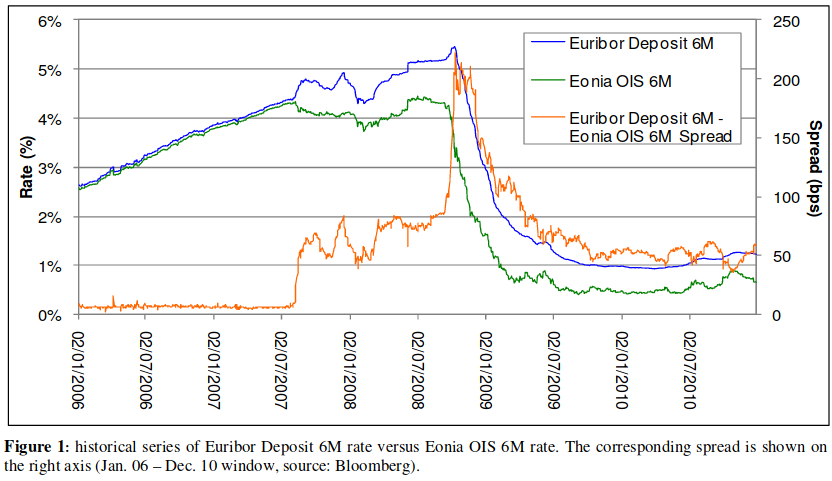
\includegraphics{credit_crunch.png}

In August 2007 however we observe a sudden increase of the Euribor rate
and a simultaneous decrease of the OIS rate that leads to the explosion
of the corresponding basis spread, touching the peak of 222 bps in
October 2008, when Lehman Brothers filed for bankruptcy protection.
Successively the basis has sensibly reduced and stabilized between 40
bps and 60 bps (notice that the pre-crisis level has never been
recovered). The same effect is observed for other similar couples,
e.g.~Euribor 3M vs OIS 3M.

The reason of the abrupt divergence between the Euribor and OIS rates
can be explained by considering both the monetary policy decisions
adopted by international authorities in response to the financial
turmoil, and the impact of the credit crunch on the credit and liquidity
risk perception of the market, coupled with the different financial
meaning and dynamics of these rates.

\begin{itemize}
\tightlist
\item
  The Euribor rate is the reference rate for over-the-counter (OTC)
  transactions in the Euro area. It is defined as ``the rate at which
  Euro interbank Deposits are being offered within the EMU zone by one
  prime bank to another at 11:00 a.m. Brussels time''. The rate fixings
  for a strip of 15 maturities, ranging from one day to one year, are
  constructed as the average of the rates submitted (excluding the
  highest and lowest 15\% tails) by a panel of banks 42 banks, selected
  among the EU banks with the highest volume of business in the Euro
  zone money markets, plus some large international bank from non-EU
  countries with important euro zone operations. \textbf{Thus, Euribor
  rates reflect the average cost of funding of banks in the interbank
  market at each given maturity. During the crisis the solvency and
  solidity of the whole financial sector was brought into question and
  the credit and liquidity risk and premia associated to interbank
  counterparties sharply increased.} The Euribor rates immediately
  reflected these dynamics and raise to their highest values over more
  than 10 years. As seen in the plot above, the Euribor 6M rate suddenly
  increased on August 2007 and reached 5.49\% on 10th October 2008.
\item
  The Eonia rate is the reference rate for overnight OTC transactions in
  the Euro area. It is constructed as the average rate of the overnight
  transactions (one day maturity deposits) executed during a given
  business day by a panel of banks on the interbank money market,
  weighted with the corresponding transaction volumes. \textbf{The Eonia
  Contribution Panel coincides with the Euribor Contribution Panel, thus
  Eonia rate includes information on the short term (overnight)
  liquidity expectations of banks in the Euro money market. It is also
  used by the European Central Bank (ECB) as a method of effecting and
  observing the transmission of its monetary policy actions. During the
  crisis the central banks were mainly concerned about restabilising the
  level of liquidity in the market, thus they reduced the level of the
  official rates.} Furthermore, the daily tenor of the Eonia rate makes
  negligible the credit and liquidity risks reflected on it: for this
  reason the OIS rates are considered the best proxies available in the
  market for the risk-free rate.
\end{itemize}

As a practial result, after the 2008 financial crisis, it is not
possible anymore to use a single discount curve to correctly price
forward rates of all tenors. For example, if we want to calculate the
net present value of a forward 6-month libor coupon, we need to
simultaneously use two different discount curves:

\begin{itemize}
\tightlist
\item
  the 6-month libor curve for determining the forward rate
\item
  the EONIA curve for discounting the expected cash flow
\end{itemize}

Essentially we are now going to explore how to implement the following
calculation:

\[\mathrm{NPV} = D_{\mathrm{EONIA}}(T_1) \times \frac{1}{T_2-T_1}\Big(\frac{D_{\mathrm{LIBOR}}(T_1)}{D_{\mathrm{LIBOR}}(T_2)} - 1 \Big)\]


However, as we have seen, Python allows you to represent collections of
objects with dictionaries. A clear improvement could be, instead of
passing a long list of data parameters to each function call, to group
the datasets into dictionaries, and then pass those to the function.
    This design pattern, i.e.~using dictionaries to group together data, and
then having functions operate on those dictionaries, perhaps with a few
additional parameters, is so useful that Python (and many other
programming languages) have a built-in feature that allows you to do
this conveniently: \textbf{classes}.
So now that we have an idea of what a class is, try to write a
\texttt{DiscountCurve} class which contains the pillar dates and pillar
discount factors as attributes and which has methods for calculating the
discount factor and forward rate at arbitrary dates.

\hypertarget{solution}{%
\paragraph{Solution:}\label{solution}}

    \begin{Verbatim}[commandchars=\\\{\}]
{\color{incolor}In [{\color{incolor}4}]:} \PY{k+kn}{import} \PY{n+nn}{math}
        \PY{k+kn}{import} \PY{n+nn}{numpy}
        \PY{k+kn}{from} \PY{n+nn}{datetime} \PY{k}{import} \PY{n}{date}
        
        \PY{k}{class} \PY{n+nc}{DiscountCurve}\PY{p}{:}
        
            \PY{c+c1}{\PYZsh{} the special \PYZus{}\PYZus{}init\PYZus{}\PYZus{} method defines }
            \PY{c+c1}{\PYZsh{} how to construct instances of the class}
            \PY{k}{def} \PY{n+nf}{\PYZus{}\PYZus{}init\PYZus{}\PYZus{}}\PY{p}{(}\PY{n+nb+bp}{self}\PY{p}{,} \PY{n}{today}\PY{p}{,} \PY{n}{pillar\PYZus{}dates}\PY{p}{,} \PY{n}{discount\PYZus{}factors}\PY{p}{)}\PY{p}{:}
                \PY{c+c1}{\PYZsh{} we just store the arguments as attributes of the instance}
                \PY{n+nb+bp}{self}\PY{o}{.}\PY{n}{today} \PY{o}{=} \PY{n}{today}
                \PY{n+nb+bp}{self}\PY{o}{.}\PY{n}{pillar\PYZus{}dates} \PY{o}{=} \PY{n}{pillar\PYZus{}dates}
                \PY{n+nb+bp}{self}\PY{o}{.}\PY{n}{discount\PYZus{}factors} \PY{o}{=} \PY{n}{discount\PYZus{}factors}
        
            \PY{c+c1}{\PYZsh{} calculates a discount factor at an arbitrary }
            \PY{c+c1}{\PYZsh{}value date using the data stored in the instance}
            \PY{k}{def} \PY{n+nf}{df}\PY{p}{(}\PY{n+nb+bp}{self}\PY{p}{,} \PY{n}{d}\PY{p}{)}\PY{p}{:}
                \PY{c+c1}{\PYZsh{} these remain local variables, }
                \PY{c+c1}{\PYZsh{} i.e. they are only available within the function.}
                \PY{c+c1}{\PYZsh{} to read (or write) instance attributes, }
                \PY{c+c1}{\PYZsh{} you always need to use the self. syntax}
                \PY{n}{log\PYZus{}discount\PYZus{}factors} \PY{o}{=} \PYZbs{}
                  \PY{p}{[}\PY{n}{math}\PY{o}{.}\PY{n}{log}\PY{p}{(}\PY{n}{discount\PYZus{}factor}\PY{p}{)} 
                   \PY{k}{for} \PY{n}{discount\PYZus{}factor} \PY{o+ow}{in} \PY{n+nb+bp}{self}\PY{o}{.}\PY{n}{discount\PYZus{}factors}\PY{p}{]}
                \PY{n}{pillar\PYZus{}days} \PY{o}{=} \PY{p}{[}\PY{p}{(}\PY{n}{pillar\PYZus{}date} \PY{o}{\PYZhy{}} \PY{n+nb+bp}{self}\PY{o}{.}\PY{n}{today}\PY{p}{)}\PY{o}{.}\PY{n}{days} 
                               \PY{k}{for} \PY{n}{pillar\PYZus{}date} \PY{o+ow}{in} \PY{n+nb+bp}{self}\PY{o}{.}\PY{n}{pillar\PYZus{}dates}\PY{p}{]}
                \PY{n}{d\PYZus{}days} \PY{o}{=} \PY{p}{(}\PY{n}{d} \PY{o}{\PYZhy{}} \PY{n+nb+bp}{self}\PY{o}{.}\PY{n}{today}\PY{p}{)}\PY{o}{.}\PY{n}{days}
                \PY{n}{interpolated\PYZus{}log\PYZus{}discount\PYZus{}factor} \PY{o}{=} \PYZbs{}
                    \PY{n}{numpy}\PY{o}{.}\PY{n}{interp}\PY{p}{(}\PY{n}{d\PYZus{}days}\PY{p}{,} \PY{n}{pillar\PYZus{}days}\PY{p}{,} \PY{n}{log\PYZus{}discount\PYZus{}factors}\PY{p}{)}
                \PY{k}{return} \PY{n}{math}\PY{o}{.}\PY{n}{exp}\PY{p}{(}\PY{n}{interpolated\PYZus{}log\PYZus{}discount\PYZus{}factor}\PY{p}{)}
        
            \PY{c+c1}{\PYZsh{} calculates a forward libor rate based on the discount }
            \PY{c+c1}{\PYZsh{} curve data stored in the instance}
            \PY{k}{def} \PY{n+nf}{forward\PYZus{}rate}\PY{p}{(}\PY{n+nb+bp}{self}\PY{p}{,} \PY{n}{d1}\PY{p}{,} \PY{n}{d2}\PY{p}{)}\PY{p}{:}
                \PY{c+c1}{\PYZsh{} we use the df method of the current instance to calculate}
                \PY{c+c1}{\PYZsh{} the forward rate}
                \PY{k}{return} \PY{p}{(}\PY{n+nb+bp}{self}\PY{o}{.}\PY{n}{df}\PY{p}{(}\PY{n}{d1}\PY{p}{)} \PY{o}{/} \PY{n+nb+bp}{self}\PY{o}{.}\PY{n}{df}\PY{p}{(}\PY{n}{d2}\PY{p}{)} \PY{o}{\PYZhy{}} \PY{l+m+mf}{1.0}\PY{p}{)} \PY{o}{*} \PYZbs{}
                        \PY{p}{(}\PY{l+m+mf}{365.0} \PY{o}{/} \PY{p}{(}\PY{p}{(}\PY{n}{d2} \PY{o}{\PYZhy{}} \PY{n}{d1}\PY{p}{)}\PY{o}{.}\PY{n}{days}\PY{p}{)}\PY{p}{)}
\end{Verbatim}

    \begin{Verbatim}[commandchars=\\\{\}]
{\color{incolor}In [{\color{incolor}5}]:} \PY{c+c1}{\PYZsh{} build the EONIA curve object}
        \PY{c+c1}{\PYZsh{} n.b. here we use the \PYZsq{}parameter=argument\PYZsq{} syntax }
        \PY{c+c1}{\PYZsh{} (today=..., pillar\PYZus{}dates=...)}
        \PY{c+c1}{\PYZsh{} just so it\PYZsq{}s really clear what we\PYZsq{}re doing - it\PYZsq{}s not necessary, }
        \PY{c+c1}{\PYZsh{} it\PYZsq{}s only for clarity}
        \PY{n}{eonia\PYZus{}curve} \PY{o}{=} \PY{n}{DiscountCurve}\PY{p}{(}\PY{n}{today}\PY{o}{=}\PY{n}{date}\PY{p}{(}\PY{l+m+mi}{2019}\PY{p}{,} \PY{l+m+mi}{10}\PY{p}{,} \PY{l+m+mi}{1}\PY{p}{)}\PY{p}{,}
                                    \PY{n}{pillar\PYZus{}dates}\PY{o}{=}\PY{p}{[}\PY{n}{date}\PY{p}{(}\PY{l+m+mi}{2019}\PY{p}{,} \PY{l+m+mi}{10}\PY{p}{,} \PY{l+m+mi}{1}\PY{p}{)}\PY{p}{,} 
                                                  \PY{n}{date}\PY{p}{(}\PY{l+m+mi}{2020}\PY{p}{,} \PY{l+m+mi}{10}\PY{p}{,} \PY{l+m+mi}{1}\PY{p}{)}\PY{p}{,} 
                                                  \PY{n}{date}\PY{p}{(}\PY{l+m+mi}{2021}\PY{p}{,} \PY{l+m+mi}{10}\PY{p}{,} \PY{l+m+mi}{1}\PY{p}{)}\PY{p}{]}\PY{p}{,}
                                    \PY{n}{discount\PYZus{}factors}\PY{o}{=}\PY{p}{[}\PY{l+m+mf}{1.0}\PY{p}{,} \PY{l+m+mf}{0.95}\PY{p}{,} \PY{l+m+mf}{0.8}\PY{p}{]}\PY{p}{)}
        
        \PY{c+c1}{\PYZsh{} build the Libor curve object}
        \PY{n}{libor\PYZus{}curve} \PY{o}{=} \PY{n}{DiscountCurve}\PY{p}{(}\PY{n}{today}\PY{o}{=}\PY{n}{date}\PY{p}{(}\PY{l+m+mi}{2019}\PY{p}{,} \PY{l+m+mi}{10}\PY{p}{,} \PY{l+m+mi}{1}\PY{p}{)}\PY{p}{,}
                                    \PY{n}{pillar\PYZus{}dates}\PY{o}{=}\PY{p}{[}\PY{n}{date}\PY{p}{(}\PY{l+m+mi}{2019}\PY{p}{,} \PY{l+m+mi}{10}\PY{p}{,} \PY{l+m+mi}{1}\PY{p}{)}\PY{p}{,} 
                                                  \PY{n}{date}\PY{p}{(}\PY{l+m+mi}{2020}\PY{p}{,} \PY{l+m+mi}{4}\PY{p}{,} \PY{l+m+mi}{1}\PY{p}{)}\PY{p}{,} 
                                                  \PY{n}{date}\PY{p}{(}\PY{l+m+mi}{2020}\PY{p}{,} \PY{l+m+mi}{10}\PY{p}{,} \PY{l+m+mi}{1}\PY{p}{)}\PY{p}{]}\PY{p}{,}
                                    \PY{n}{discount\PYZus{}factors}\PY{o}{=}\PY{p}{[}\PY{l+m+mf}{1.0}\PY{p}{,} \PY{l+m+mf}{0.98}\PY{p}{,} \PY{l+m+mf}{0.82}\PY{p}{]}\PY{p}{)}
        
        \PY{c+c1}{\PYZsh{} Let\PYZsq{}s compute the discount factor of the two curves}
        \PY{c+c1}{\PYZsh{} on the 2020\PYZhy{}5\PYZhy{}1}
        \PY{n+nb}{print} \PY{p}{(}\PY{n}{eonia\PYZus{}curve}\PY{o}{.}\PY{n}{df}\PY{p}{(}\PY{n}{date}\PY{p}{(}\PY{l+m+mi}{2020}\PY{p}{,} \PY{l+m+mi}{5}\PY{p}{,} \PY{l+m+mi}{1}\PY{p}{)}\PY{p}{)}\PY{p}{)}
        \PY{n+nb}{print} \PY{p}{(}\PY{n}{libor\PYZus{}curve}\PY{o}{.}\PY{n}{df}\PY{p}{(}\PY{n}{date}\PY{p}{(}\PY{l+m+mi}{2020}\PY{p}{,} \PY{l+m+mi}{5}\PY{p}{,} \PY{l+m+mi}{1}\PY{p}{)}\PY{p}{)}\PY{p}{)}
\end{Verbatim}

    \begin{Verbatim}[commandchars=\\\{\}]
0.9705901255781632
0.9517777485424973

    \end{Verbatim}

    \begin{Verbatim}[commandchars=\\\{\}]
{\color{incolor}In [{\color{incolor}6}]:} \PY{c+c1}{\PYZsh{} Let\PYZsq{}s compute now the 6m forward rate at 1\PYZhy{}4\PYZhy{}2020}
        \PY{n+nb}{print} \PY{p}{(}\PY{n}{eonia\PYZus{}curve}\PY{o}{.}\PY{n}{forward\PYZus{}rate}\PY{p}{(}\PY{n}{date}\PY{p}{(}\PY{l+m+mi}{2019}\PY{p}{,} \PY{l+m+mi}{10}\PY{p}{,} \PY{l+m+mi}{1}\PY{p}{)}\PY{p}{,} 
                                         \PY{n}{date}\PY{p}{(}\PY{l+m+mi}{2020}\PY{p}{,} \PY{l+m+mi}{10}\PY{p}{,} \PY{l+m+mi}{1}\PY{p}{)}\PY{p}{)}\PY{p}{)}
        
        \PY{n+nb}{print} \PY{p}{(}\PY{n}{libor\PYZus{}curve}\PY{o}{.}\PY{n}{forward\PYZus{}rate}\PY{p}{(}\PY{n}{date}\PY{p}{(}\PY{l+m+mi}{2020}\PY{p}{,} \PY{l+m+mi}{4}\PY{p}{,} \PY{l+m+mi}{1}\PY{p}{)}\PY{p}{,} 
                                         \PY{n}{date}\PY{p}{(}\PY{l+m+mi}{2020}\PY{p}{,} \PY{l+m+mi}{10}\PY{p}{,} \PY{l+m+mi}{1}\PY{p}{)}\PY{p}{)}\PY{p}{)}
\end{Verbatim}

    \begin{Verbatim}[commandchars=\\\{\}]
0.05248777681909687
0.3891776622684259

    \end{Verbatim}

    \begin{Verbatim}[commandchars=\\\{\}]
{\color{incolor}In [{\color{incolor}7}]:} \PY{c+c1}{\PYZsh{} Compute the NPV of the 6m forward libor coupon}
        \PY{n}{npv} \PY{o}{=} \PY{n}{eonia\PYZus{}curve}\PY{o}{.}\PY{n}{df}\PY{p}{(}\PY{n}{date}\PY{p}{(}\PY{l+m+mi}{2020}\PY{p}{,} \PY{l+m+mi}{4}\PY{p}{,} \PY{l+m+mi}{1}\PY{p}{)}\PY{p}{)} \PY{o}{*} \PYZbs{}
              \PY{n}{libor\PYZus{}curve}\PY{o}{.}\PY{n}{forward\PYZus{}rate}\PY{p}{(}\PY{n}{date}\PY{p}{(}\PY{l+m+mi}{2020}\PY{p}{,}\PY{l+m+mi}{4}\PY{p}{,} \PY{l+m+mi}{1}\PY{p}{)}\PY{p}{,} 
                                        \PY{n}{date}\PY{p}{(}\PY{l+m+mi}{2020}\PY{p}{,} \PY{l+m+mi}{10}\PY{p}{,} \PY{l+m+mi}{1}\PY{p}{)}\PY{p}{)}
        
        \PY{c+c1}{\PYZsh{} Compute it in the pre\PYZhy{}2008 way}
        \PY{n}{npv\PYZus{}pre\PYZus{}2008} \PY{o}{=} \PY{n}{libor\PYZus{}curve}\PY{o}{.}\PY{n}{df}\PY{p}{(}\PY{n}{date}\PY{p}{(}\PY{l+m+mi}{2020}\PY{p}{,} \PY{l+m+mi}{4}\PY{p}{,} \PY{l+m+mi}{1}\PY{p}{)}\PY{p}{)} \PY{o}{*} \PYZbs{}
                       \PY{n}{libor\PYZus{}curve}\PY{o}{.}\PY{n}{forward\PYZus{}rate}\PY{p}{(}\PY{n}{date}\PY{p}{(}\PY{l+m+mi}{2020}\PY{p}{,} \PY{l+m+mi}{4}\PY{p}{,} \PY{l+m+mi}{1}\PY{p}{)}\PY{p}{,} 
                                                 \PY{n}{date}\PY{p}{(}\PY{l+m+mi}{2020}\PY{p}{,} \PY{l+m+mi}{10}\PY{p}{,} \PY{l+m+mi}{1}\PY{p}{)}\PY{p}{)}
        \PY{n+nb}{print} \PY{p}{(}\PY{n}{npv}\PY{p}{)}
        \PY{n+nb}{print} \PY{p}{(}\PY{n}{npv\PYZus{}pre\PYZus{}2008}\PY{p}{)}
\end{Verbatim}

    \begin{Verbatim}[commandchars=\\\{\}]
0.37932346377238657
0.38139410902305737

    \end{Verbatim}


\clearpage

% Default to the notebook output style

    


% Inherit from the specified cell style.




    
\documentclass[11pt]{article}

    
    
    \usepackage[T1]{fontenc}
    % Nicer default font (+ math font) than Computer Modern for most use cases
    \usepackage{mathpazo}

    % Basic figure setup, for now with no caption control since it's done
    % automatically by Pandoc (which extracts ![](path) syntax from Markdown).
    \usepackage{graphicx}
    % We will generate all images so they have a width \maxwidth. This means
    % that they will get their normal width if they fit onto the page, but
    % are scaled down if they would overflow the margins.
    \makeatletter
    \def\maxwidth{\ifdim\Gin@nat@width>\linewidth\linewidth
    \else\Gin@nat@width\fi}
    \makeatother
    \let\Oldincludegraphics\includegraphics
    % Set max figure width to be 80% of text width, for now hardcoded.
    \renewcommand{\includegraphics}[1]{\Oldincludegraphics[width=.8\maxwidth]{#1}}
    % Ensure that by default, figures have no caption (until we provide a
    % proper Figure object with a Caption API and a way to capture that
    % in the conversion process - todo).
    \usepackage{caption}
    \DeclareCaptionLabelFormat{nolabel}{}
    \captionsetup{labelformat=nolabel}

    \usepackage{adjustbox} % Used to constrain images to a maximum size 
    \usepackage{xcolor} % Allow colors to be defined
    \usepackage{enumerate} % Needed for markdown enumerations to work
    \usepackage{geometry} % Used to adjust the document margins
    \usepackage{amsmath} % Equations
    \usepackage{amssymb} % Equations
    \usepackage{textcomp} % defines textquotesingle
    % Hack from http://tex.stackexchange.com/a/47451/13684:
    \AtBeginDocument{%
        \def\PYZsq{\textquotesingle}% Upright quotes in Pygmentized code
    }
    \usepackage{upquote} % Upright quotes for verbatim code
    \usepackage{eurosym} % defines \euro
    \usepackage[mathletters]{ucs} % Extended unicode (utf-8) support
    \usepackage[utf8x]{inputenc} % Allow utf-8 characters in the tex document
    \usepackage{fancyvrb} % verbatim replacement that allows latex
    \usepackage{grffile} % extends the file name processing of package graphics 
                         % to support a larger range 
    % The hyperref package gives us a pdf with properly built
    % internal navigation ('pdf bookmarks' for the table of contents,
    % internal cross-reference links, web links for URLs, etc.)
    \usepackage{hyperref}
    \usepackage{longtable} % longtable support required by pandoc >1.10
    \usepackage{booktabs}  % table support for pandoc > 1.12.2
    \usepackage[inline]{enumitem} % IRkernel/repr support (it uses the enumerate* environment)
    \usepackage[normalem]{ulem} % ulem is needed to support strikethroughs (\sout)
                                % normalem makes italics be italics, not underlines
    \usepackage{mathrsfs}
    

    
    
    % Colors for the hyperref package
    \definecolor{urlcolor}{rgb}{0,.145,.698}
    \definecolor{linkcolor}{rgb}{.71,0.21,0.01}
    \definecolor{citecolor}{rgb}{.12,.54,.11}

    % ANSI colors
    \definecolor{ansi-black}{HTML}{3E424D}
    \definecolor{ansi-black-intense}{HTML}{282C36}
    \definecolor{ansi-red}{HTML}{E75C58}
    \definecolor{ansi-red-intense}{HTML}{B22B31}
    \definecolor{ansi-green}{HTML}{00A250}
    \definecolor{ansi-green-intense}{HTML}{007427}
    \definecolor{ansi-yellow}{HTML}{DDB62B}
    \definecolor{ansi-yellow-intense}{HTML}{B27D12}
    \definecolor{ansi-blue}{HTML}{208FFB}
    \definecolor{ansi-blue-intense}{HTML}{0065CA}
    \definecolor{ansi-magenta}{HTML}{D160C4}
    \definecolor{ansi-magenta-intense}{HTML}{A03196}
    \definecolor{ansi-cyan}{HTML}{60C6C8}
    \definecolor{ansi-cyan-intense}{HTML}{258F8F}
    \definecolor{ansi-white}{HTML}{C5C1B4}
    \definecolor{ansi-white-intense}{HTML}{A1A6B2}
    \definecolor{ansi-default-inverse-fg}{HTML}{FFFFFF}
    \definecolor{ansi-default-inverse-bg}{HTML}{000000}

    % commands and environments needed by pandoc snippets
    % extracted from the output of `pandoc -s`
    \providecommand{\tightlist}{%
      \setlength{\itemsep}{0pt}\setlength{\parskip}{0pt}}
    \DefineVerbatimEnvironment{Highlighting}{Verbatim}{commandchars=\\\{\}}
    % Add ',fontsize=\small' for more characters per line
    \newenvironment{Shaded}{}{}
    \newcommand{\KeywordTok}[1]{\textcolor[rgb]{0.00,0.44,0.13}{\textbf{{#1}}}}
    \newcommand{\DataTypeTok}[1]{\textcolor[rgb]{0.56,0.13,0.00}{{#1}}}
    \newcommand{\DecValTok}[1]{\textcolor[rgb]{0.25,0.63,0.44}{{#1}}}
    \newcommand{\BaseNTok}[1]{\textcolor[rgb]{0.25,0.63,0.44}{{#1}}}
    \newcommand{\FloatTok}[1]{\textcolor[rgb]{0.25,0.63,0.44}{{#1}}}
    \newcommand{\CharTok}[1]{\textcolor[rgb]{0.25,0.44,0.63}{{#1}}}
    \newcommand{\StringTok}[1]{\textcolor[rgb]{0.25,0.44,0.63}{{#1}}}
    \newcommand{\CommentTok}[1]{\textcolor[rgb]{0.38,0.63,0.69}{\textit{{#1}}}}
    \newcommand{\OtherTok}[1]{\textcolor[rgb]{0.00,0.44,0.13}{{#1}}}
    \newcommand{\AlertTok}[1]{\textcolor[rgb]{1.00,0.00,0.00}{\textbf{{#1}}}}
    \newcommand{\FunctionTok}[1]{\textcolor[rgb]{0.02,0.16,0.49}{{#1}}}
    \newcommand{\RegionMarkerTok}[1]{{#1}}
    \newcommand{\ErrorTok}[1]{\textcolor[rgb]{1.00,0.00,0.00}{\textbf{{#1}}}}
    \newcommand{\NormalTok}[1]{{#1}}
    
    % Additional commands for more recent versions of Pandoc
    \newcommand{\ConstantTok}[1]{\textcolor[rgb]{0.53,0.00,0.00}{{#1}}}
    \newcommand{\SpecialCharTok}[1]{\textcolor[rgb]{0.25,0.44,0.63}{{#1}}}
    \newcommand{\VerbatimStringTok}[1]{\textcolor[rgb]{0.25,0.44,0.63}{{#1}}}
    \newcommand{\SpecialStringTok}[1]{\textcolor[rgb]{0.73,0.40,0.53}{{#1}}}
    \newcommand{\ImportTok}[1]{{#1}}
    \newcommand{\DocumentationTok}[1]{\textcolor[rgb]{0.73,0.13,0.13}{\textit{{#1}}}}
    \newcommand{\AnnotationTok}[1]{\textcolor[rgb]{0.38,0.63,0.69}{\textbf{\textit{{#1}}}}}
    \newcommand{\CommentVarTok}[1]{\textcolor[rgb]{0.38,0.63,0.69}{\textbf{\textit{{#1}}}}}
    \newcommand{\VariableTok}[1]{\textcolor[rgb]{0.10,0.09,0.49}{{#1}}}
    \newcommand{\ControlFlowTok}[1]{\textcolor[rgb]{0.00,0.44,0.13}{\textbf{{#1}}}}
    \newcommand{\OperatorTok}[1]{\textcolor[rgb]{0.40,0.40,0.40}{{#1}}}
    \newcommand{\BuiltInTok}[1]{{#1}}
    \newcommand{\ExtensionTok}[1]{{#1}}
    \newcommand{\PreprocessorTok}[1]{\textcolor[rgb]{0.74,0.48,0.00}{{#1}}}
    \newcommand{\AttributeTok}[1]{\textcolor[rgb]{0.49,0.56,0.16}{{#1}}}
    \newcommand{\InformationTok}[1]{\textcolor[rgb]{0.38,0.63,0.69}{\textbf{\textit{{#1}}}}}
    \newcommand{\WarningTok}[1]{\textcolor[rgb]{0.38,0.63,0.69}{\textbf{\textit{{#1}}}}}
    
    
    % Define a nice break command that doesn't care if a line doesn't already
    % exist.
    \def\br{\hspace*{\fill} \\* }
    % Math Jax compatibility definitions
    \def\gt{>}
    \def\lt{<}
    \let\Oldtex\TeX
    \let\Oldlatex\LaTeX
    \renewcommand{\TeX}{\textrm{\Oldtex}}
    \renewcommand{\LaTeX}{\textrm{\Oldlatex}}
    % Document parameters
    % Document title
    \title{Swaps and Modules - Practical Lesson 5}
    \author{Matteo Sani \\ \href{mailto:matteosan1@gmail.com}{matteosan1@gmail.com}}
    
    
    
    

    % Pygments definitions
    
\makeatletter
\def\PY@reset{\let\PY@it=\relax \let\PY@bf=\relax%
    \let\PY@ul=\relax \let\PY@tc=\relax%
    \let\PY@bc=\relax \let\PY@ff=\relax}
\def\PY@tok#1{\csname PY@tok@#1\endcsname}
\def\PY@toks#1+{\ifx\relax#1\empty\else%
    \PY@tok{#1}\expandafter\PY@toks\fi}
\def\PY@do#1{\PY@bc{\PY@tc{\PY@ul{%
    \PY@it{\PY@bf{\PY@ff{#1}}}}}}}
\def\PY#1#2{\PY@reset\PY@toks#1+\relax+\PY@do{#2}}

\expandafter\def\csname PY@tok@w\endcsname{\def\PY@tc##1{\textcolor[rgb]{0.73,0.73,0.73}{##1}}}
\expandafter\def\csname PY@tok@c\endcsname{\let\PY@it=\textit\def\PY@tc##1{\textcolor[rgb]{0.25,0.50,0.50}{##1}}}
\expandafter\def\csname PY@tok@cp\endcsname{\def\PY@tc##1{\textcolor[rgb]{0.74,0.48,0.00}{##1}}}
\expandafter\def\csname PY@tok@k\endcsname{\let\PY@bf=\textbf\def\PY@tc##1{\textcolor[rgb]{0.00,0.50,0.00}{##1}}}
\expandafter\def\csname PY@tok@kp\endcsname{\def\PY@tc##1{\textcolor[rgb]{0.00,0.50,0.00}{##1}}}
\expandafter\def\csname PY@tok@kt\endcsname{\def\PY@tc##1{\textcolor[rgb]{0.69,0.00,0.25}{##1}}}
\expandafter\def\csname PY@tok@o\endcsname{\def\PY@tc##1{\textcolor[rgb]{0.40,0.40,0.40}{##1}}}
\expandafter\def\csname PY@tok@ow\endcsname{\let\PY@bf=\textbf\def\PY@tc##1{\textcolor[rgb]{0.67,0.13,1.00}{##1}}}
\expandafter\def\csname PY@tok@nb\endcsname{\def\PY@tc##1{\textcolor[rgb]{0.00,0.50,0.00}{##1}}}
\expandafter\def\csname PY@tok@nf\endcsname{\def\PY@tc##1{\textcolor[rgb]{0.00,0.00,1.00}{##1}}}
\expandafter\def\csname PY@tok@nc\endcsname{\let\PY@bf=\textbf\def\PY@tc##1{\textcolor[rgb]{0.00,0.00,1.00}{##1}}}
\expandafter\def\csname PY@tok@nn\endcsname{\let\PY@bf=\textbf\def\PY@tc##1{\textcolor[rgb]{0.00,0.00,1.00}{##1}}}
\expandafter\def\csname PY@tok@ne\endcsname{\let\PY@bf=\textbf\def\PY@tc##1{\textcolor[rgb]{0.82,0.25,0.23}{##1}}}
\expandafter\def\csname PY@tok@nv\endcsname{\def\PY@tc##1{\textcolor[rgb]{0.10,0.09,0.49}{##1}}}
\expandafter\def\csname PY@tok@no\endcsname{\def\PY@tc##1{\textcolor[rgb]{0.53,0.00,0.00}{##1}}}
\expandafter\def\csname PY@tok@nl\endcsname{\def\PY@tc##1{\textcolor[rgb]{0.63,0.63,0.00}{##1}}}
\expandafter\def\csname PY@tok@ni\endcsname{\let\PY@bf=\textbf\def\PY@tc##1{\textcolor[rgb]{0.60,0.60,0.60}{##1}}}
\expandafter\def\csname PY@tok@na\endcsname{\def\PY@tc##1{\textcolor[rgb]{0.49,0.56,0.16}{##1}}}
\expandafter\def\csname PY@tok@nt\endcsname{\let\PY@bf=\textbf\def\PY@tc##1{\textcolor[rgb]{0.00,0.50,0.00}{##1}}}
\expandafter\def\csname PY@tok@nd\endcsname{\def\PY@tc##1{\textcolor[rgb]{0.67,0.13,1.00}{##1}}}
\expandafter\def\csname PY@tok@s\endcsname{\def\PY@tc##1{\textcolor[rgb]{0.73,0.13,0.13}{##1}}}
\expandafter\def\csname PY@tok@sd\endcsname{\let\PY@it=\textit\def\PY@tc##1{\textcolor[rgb]{0.73,0.13,0.13}{##1}}}
\expandafter\def\csname PY@tok@si\endcsname{\let\PY@bf=\textbf\def\PY@tc##1{\textcolor[rgb]{0.73,0.40,0.53}{##1}}}
\expandafter\def\csname PY@tok@se\endcsname{\let\PY@bf=\textbf\def\PY@tc##1{\textcolor[rgb]{0.73,0.40,0.13}{##1}}}
\expandafter\def\csname PY@tok@sr\endcsname{\def\PY@tc##1{\textcolor[rgb]{0.73,0.40,0.53}{##1}}}
\expandafter\def\csname PY@tok@ss\endcsname{\def\PY@tc##1{\textcolor[rgb]{0.10,0.09,0.49}{##1}}}
\expandafter\def\csname PY@tok@sx\endcsname{\def\PY@tc##1{\textcolor[rgb]{0.00,0.50,0.00}{##1}}}
\expandafter\def\csname PY@tok@m\endcsname{\def\PY@tc##1{\textcolor[rgb]{0.40,0.40,0.40}{##1}}}
\expandafter\def\csname PY@tok@gh\endcsname{\let\PY@bf=\textbf\def\PY@tc##1{\textcolor[rgb]{0.00,0.00,0.50}{##1}}}
\expandafter\def\csname PY@tok@gu\endcsname{\let\PY@bf=\textbf\def\PY@tc##1{\textcolor[rgb]{0.50,0.00,0.50}{##1}}}
\expandafter\def\csname PY@tok@gd\endcsname{\def\PY@tc##1{\textcolor[rgb]{0.63,0.00,0.00}{##1}}}
\expandafter\def\csname PY@tok@gi\endcsname{\def\PY@tc##1{\textcolor[rgb]{0.00,0.63,0.00}{##1}}}
\expandafter\def\csname PY@tok@gr\endcsname{\def\PY@tc##1{\textcolor[rgb]{1.00,0.00,0.00}{##1}}}
\expandafter\def\csname PY@tok@ge\endcsname{\let\PY@it=\textit}
\expandafter\def\csname PY@tok@gs\endcsname{\let\PY@bf=\textbf}
\expandafter\def\csname PY@tok@gp\endcsname{\let\PY@bf=\textbf\def\PY@tc##1{\textcolor[rgb]{0.00,0.00,0.50}{##1}}}
\expandafter\def\csname PY@tok@go\endcsname{\def\PY@tc##1{\textcolor[rgb]{0.53,0.53,0.53}{##1}}}
\expandafter\def\csname PY@tok@gt\endcsname{\def\PY@tc##1{\textcolor[rgb]{0.00,0.27,0.87}{##1}}}
\expandafter\def\csname PY@tok@err\endcsname{\def\PY@bc##1{\setlength{\fboxsep}{0pt}\fcolorbox[rgb]{1.00,0.00,0.00}{1,1,1}{\strut ##1}}}
\expandafter\def\csname PY@tok@kc\endcsname{\let\PY@bf=\textbf\def\PY@tc##1{\textcolor[rgb]{0.00,0.50,0.00}{##1}}}
\expandafter\def\csname PY@tok@kd\endcsname{\let\PY@bf=\textbf\def\PY@tc##1{\textcolor[rgb]{0.00,0.50,0.00}{##1}}}
\expandafter\def\csname PY@tok@kn\endcsname{\let\PY@bf=\textbf\def\PY@tc##1{\textcolor[rgb]{0.00,0.50,0.00}{##1}}}
\expandafter\def\csname PY@tok@kr\endcsname{\let\PY@bf=\textbf\def\PY@tc##1{\textcolor[rgb]{0.00,0.50,0.00}{##1}}}
\expandafter\def\csname PY@tok@bp\endcsname{\def\PY@tc##1{\textcolor[rgb]{0.00,0.50,0.00}{##1}}}
\expandafter\def\csname PY@tok@fm\endcsname{\def\PY@tc##1{\textcolor[rgb]{0.00,0.00,1.00}{##1}}}
\expandafter\def\csname PY@tok@vc\endcsname{\def\PY@tc##1{\textcolor[rgb]{0.10,0.09,0.49}{##1}}}
\expandafter\def\csname PY@tok@vg\endcsname{\def\PY@tc##1{\textcolor[rgb]{0.10,0.09,0.49}{##1}}}
\expandafter\def\csname PY@tok@vi\endcsname{\def\PY@tc##1{\textcolor[rgb]{0.10,0.09,0.49}{##1}}}
\expandafter\def\csname PY@tok@vm\endcsname{\def\PY@tc##1{\textcolor[rgb]{0.10,0.09,0.49}{##1}}}
\expandafter\def\csname PY@tok@sa\endcsname{\def\PY@tc##1{\textcolor[rgb]{0.73,0.13,0.13}{##1}}}
\expandafter\def\csname PY@tok@sb\endcsname{\def\PY@tc##1{\textcolor[rgb]{0.73,0.13,0.13}{##1}}}
\expandafter\def\csname PY@tok@sc\endcsname{\def\PY@tc##1{\textcolor[rgb]{0.73,0.13,0.13}{##1}}}
\expandafter\def\csname PY@tok@dl\endcsname{\def\PY@tc##1{\textcolor[rgb]{0.73,0.13,0.13}{##1}}}
\expandafter\def\csname PY@tok@s2\endcsname{\def\PY@tc##1{\textcolor[rgb]{0.73,0.13,0.13}{##1}}}
\expandafter\def\csname PY@tok@sh\endcsname{\def\PY@tc##1{\textcolor[rgb]{0.73,0.13,0.13}{##1}}}
\expandafter\def\csname PY@tok@s1\endcsname{\def\PY@tc##1{\textcolor[rgb]{0.73,0.13,0.13}{##1}}}
\expandafter\def\csname PY@tok@mb\endcsname{\def\PY@tc##1{\textcolor[rgb]{0.40,0.40,0.40}{##1}}}
\expandafter\def\csname PY@tok@mf\endcsname{\def\PY@tc##1{\textcolor[rgb]{0.40,0.40,0.40}{##1}}}
\expandafter\def\csname PY@tok@mh\endcsname{\def\PY@tc##1{\textcolor[rgb]{0.40,0.40,0.40}{##1}}}
\expandafter\def\csname PY@tok@mi\endcsname{\def\PY@tc##1{\textcolor[rgb]{0.40,0.40,0.40}{##1}}}
\expandafter\def\csname PY@tok@il\endcsname{\def\PY@tc##1{\textcolor[rgb]{0.40,0.40,0.40}{##1}}}
\expandafter\def\csname PY@tok@mo\endcsname{\def\PY@tc##1{\textcolor[rgb]{0.40,0.40,0.40}{##1}}}
\expandafter\def\csname PY@tok@ch\endcsname{\let\PY@it=\textit\def\PY@tc##1{\textcolor[rgb]{0.25,0.50,0.50}{##1}}}
\expandafter\def\csname PY@tok@cm\endcsname{\let\PY@it=\textit\def\PY@tc##1{\textcolor[rgb]{0.25,0.50,0.50}{##1}}}
\expandafter\def\csname PY@tok@cpf\endcsname{\let\PY@it=\textit\def\PY@tc##1{\textcolor[rgb]{0.25,0.50,0.50}{##1}}}
\expandafter\def\csname PY@tok@c1\endcsname{\let\PY@it=\textit\def\PY@tc##1{\textcolor[rgb]{0.25,0.50,0.50}{##1}}}
\expandafter\def\csname PY@tok@cs\endcsname{\let\PY@it=\textit\def\PY@tc##1{\textcolor[rgb]{0.25,0.50,0.50}{##1}}}

\def\PYZbs{\char`\\}
\def\PYZus{\char`\_}
\def\PYZob{\char`\{}
\def\PYZcb{\char`\}}
\def\PYZca{\char`\^}
\def\PYZam{\char`\&}
\def\PYZlt{\char`\<}
\def\PYZgt{\char`\>}
\def\PYZsh{\char`\#}
\def\PYZpc{\char`\%}
\def\PYZdl{\char`\$}
\def\PYZhy{\char`\-}
\def\PYZsq{\char`\'}
\def\PYZdq{\char`\"}
\def\PYZti{\char`\~}
% for compatibility with earlier versions
\def\PYZat{@}
\def\PYZlb{[}
\def\PYZrb{]}
\makeatother


    % Exact colors from NB
    \definecolor{incolor}{rgb}{0.0, 0.0, 0.5}
    \definecolor{outcolor}{rgb}{0.545, 0.0, 0.0}



    
    % Prevent overflowing lines due to hard-to-break entities
    \sloppy 
    % Setup hyperref package
    \hypersetup{
      breaklinks=true,  % so long urls are correctly broken across lines
      colorlinks=true,
      urlcolor=urlcolor,
      linkcolor=linkcolor,
      citecolor=citecolor,
      }
    % Slightly bigger margins than the latex defaults
    
    \geometry{verbose,tmargin=1in,bmargin=1in,lmargin=1in,rmargin=1in}
    
    

    \begin{document}
    
    
    \maketitle
    
    

    
    \hypertarget{swaps-and-modules---practical-lesson-5}{%
\section{Swaps and Modules}\label{swaps-and-modules---practical-lesson-5}}

\hypertarget{recap}{%
\subsection{Recap}\label{recap}}

\begin{itemize}
\tightlist
\item
  basic Python (mostly not related directly to finance)
\item
  how to implement a discount factor interpolation function
\item
  qrapping up functionality in classes in order to work with multiple
  data sets more easily
\item
  libor forward rate calculator
\end{itemize}

\hypertarget{todays-lesson}{%
\subsection{Today's lesson}\label{todays-lesson}}

We're going to look at: * modules, and start building up our library of
finance-related functionality * implementing an Overnight Index Swap
class for calculating the NPV of an OIS.

\hypertarget{modules}{%
\section{Modules}\label{modules}}

An interactive session (e.g notebook or interactive shell) is great for
quick testing and exploratory use, but once you have some code
(i.e.~functions or classes) which you'd like to reuse often, rather than
copy/pasting it every time you need it, you can save it in a .py file
and use it from your session (aka you can create your own library).

These work just like the modules we have been importing up to now,
except they're written by us! Take a look at this video
(https://www.youtube.com/watch?v=AqCl65wxikw) for an example of how it's
done for Jupyter notebook.

We're going to start writing a module called \textbf{finmarkets}, and
over the course of the remaining lessons we'll add functionality related
to the theory lessons.

So first of all let's create a new file called finmarkets.py and copy
into it the \texttt{DiscountCurve} class we wrote last time.

    \begin{Verbatim}[commandchars=\\\{\}]
{\color{incolor}In [{\color{incolor}1}]:} \PY{k+kn}{from} \PY{n+nn}{datetime} \PY{k}{import} \PY{n}{date}
        \PY{k+kn}{from} \PY{n+nn}{finmarkets} \PY{k}{import} \PY{n}{DiscountCurve}
        
        \PY{n}{curve} \PY{o}{=} \PY{n}{DiscountCurve}\PY{p}{(}\PY{n}{date}\PY{p}{(}\PY{l+m+mi}{2019}\PY{p}{,} \PY{l+m+mi}{1}\PY{p}{,} \PY{l+m+mi}{1}\PY{p}{)}\PY{p}{,}
                              \PY{p}{[}\PY{n}{date}\PY{p}{(}\PY{l+m+mi}{2019}\PY{p}{,} \PY{l+m+mi}{1}\PY{p}{,} \PY{l+m+mi}{1}\PY{p}{)}\PY{p}{,} 
                               \PY{n}{date}\PY{p}{(}\PY{l+m+mi}{2019}\PY{p}{,} \PY{l+m+mi}{6}\PY{p}{,} \PY{l+m+mi}{1}\PY{p}{)}\PY{p}{,} 
                               \PY{n}{date}\PY{p}{(}\PY{l+m+mi}{2020}\PY{p}{,} \PY{l+m+mi}{1}\PY{p}{,} \PY{l+m+mi}{1}\PY{p}{)}\PY{p}{]}\PY{p}{,}
                              \PY{p}{[}\PY{l+m+mf}{1.0}\PY{p}{,} \PY{l+m+mf}{0.98}\PY{p}{,} \PY{l+m+mf}{0.82}\PY{p}{]}\PY{p}{)}
        \PY{n}{curve}\PY{o}{.}\PY{n}{df}\PY{p}{(}\PY{n}{date}\PY{p}{(}\PY{l+m+mi}{2019}\PY{p}{,} \PY{l+m+mi}{7}\PY{p}{,} \PY{l+m+mi}{1}\PY{p}{)}\PY{p}{)}
\end{Verbatim}

\begin{Verbatim}[commandchars=\\\{\}]
{\color{outcolor}Out[{\color{outcolor}1}]:} 0.9558151167629666
\end{Verbatim}
            
    We will use this discount curve later in this lesson.

\hypertarget{overnight-index-swap}{%
\section{Overnight Index Swap}\label{overnight-index-swap}}

Overnight Index Swap (OIS) are products which pay a floating coupon,
determined by overnight rate fixings over the reference periods, against
a fixed coupon. We will always look at these products from the point of
view of the \textbf{receiver of the floating leg}. Therefore an OIS is
defined by:

\begin{itemize}
\tightlist
\item
  a notional amount \(N\)
\item
  a start date \(d_0\)
\item
  a sequence of payment dates \(d_1,...,d_n\)
\item
  a fixed rate \(K\)
\end{itemize}

For simplicity we're assuming that the fixed and floating legs have the
same notional and payment dates, although this is not necessarily always
the case in practice.

At each payment date, the floating leg pays a cash flow determined as
follows:

\[f_{\mathrm{float},~i} = N \Bigg\{\prod_{d=d_{i-1}}^{d=d_i-1}\Big(1+r_{o/n}(d)\cdot\frac{1}{360}\Big) -1 \Bigg\}\]

(This formula is valid for an EONIA swap, i.e.~for OIS swaps in EUR,
other currencies might have different conventions. The \(\frac{1}{360}\)
fraction appears because EONIA rates are quoted using the ACT/360
daycount convention and here we're making a simplifying assumption of
ignoring weekends and holidays, so we assume that each overnight rate is
valid for only one day.)

The sum of the discounted expected values of these cashflows is

\[\mathrm{NPV}_{\mathrm{float}} = \sum_{i=1}^{n}D(d_i)\mathbb{E}[f_{\mathrm{float},~i}]\]

where \(D(d)\) is the discount factor with expiry \(d\). On the other
hand, by definition (remember practical lesson 4 with forward rates), we
also have the following relationship

\[\mathbb{E}[f_{\mathrm{float},~i}] = N\cdot\Big(\frac{D_{ois}(d_{i-1})}{D_{ois}(d_{i})} - 1\Big) \]

where \(D_{ois}(d)\) is the discount factor implied by OIS prices.

In a previous theory lesson we mentioned that the correct curve to use
for discounting the flows of a collateralized contract is the one
associated with the collateral. Since OIS contracts are collateralized
with cash, and cash accrues daily interes at the overnight rate, the OIS
curve is itself the correct curve with which to discount the flows of an
OIS contract !

In summary, \(D = D_{ois}\) so the NPV simplifies to

\[\mathrm{NPV}_{\mathrm{float}} = N\cdot\sum_{i=1}^{n}[D(d_{i-1}) - D(d_i)] = N \cdot [D(d_0) - D(d_n)]\]

Each cash flow of the fixed leg is equal to

\[f_{\mathrm{fix},~i}=N\cdot K\cdot \frac{d_i - d_{i-1}}{360}\]

so the NPV of the fixed leg is

\[\mathrm{NPV}_{\mathrm{fix}} = N\cdot K\cdot \sum_{i=1}^{n}D(d_{i})\frac{d_i - d_{i-1}}{360}\]

Ultimately the aim will be to take a series of OIS quotations, and
determine the discount factors implied by their prices. To do this we'll
build a pricing function (or rather a class), which takes discount curve
as the input and produces the net present value (NPV) of the OIS as the
output. Next lesson we'll put this function inside a numerical optimizer
to invert the process and hence to determine the implied discount
factors from the prices.

    \begin{Verbatim}[commandchars=\\\{\}]
{\color{incolor}In [{\color{incolor}2}]:} \PY{k}{class} \PY{n+nc}{OvernightIndexSwap}\PY{p}{(}\PY{n+nb}{object}\PY{p}{)}\PY{p}{:}
        
            \PY{c+c1}{\PYZsh{} this method is called to build the instance,}
            \PY{c+c1}{\PYZsh{} we take some data arguments and save them as}
            \PY{c+c1}{\PYZsh{} attributes of self }
            \PY{c+c1}{\PYZsh{} n.b.: payment\PYZus{}dates should be a list of dates,}
            \PY{c+c1}{\PYZsh{} including the start date as the first element}
            \PY{k}{def} \PY{n+nf}{\PYZus{}\PYZus{}init\PYZus{}\PYZus{}}\PY{p}{(}\PY{n+nb+bp}{self}\PY{p}{,} \PY{n}{notional}\PY{p}{,} \PY{n}{payment\PYZus{}dates}\PY{p}{,} \PY{n}{fixed\PYZus{}rate}\PY{p}{)}\PY{p}{:}
                \PY{n+nb+bp}{self}\PY{o}{.}\PY{n}{notional} \PY{o}{=} \PY{n}{notional}
                \PY{n+nb+bp}{self}\PY{o}{.}\PY{n}{payment\PYZus{}dates} \PY{o}{=} \PY{n}{payment\PYZus{}dates}
                \PY{n+nb+bp}{self}\PY{o}{.}\PY{n}{fixed\PYZus{}rate} \PY{o}{=} \PY{n}{fixed\PYZus{}rate}
                
            \PY{c+c1}{\PYZsh{} this method takes a discount curve and calculates}
            \PY{c+c1}{\PYZsh{} the NPV of the floating leg using that curve}
            \PY{k}{def} \PY{n+nf}{npv\PYZus{}floating\PYZus{}leg}\PY{p}{(}\PY{n+nb+bp}{self}\PY{p}{,} \PY{n}{discount\PYZus{}curve}\PY{p}{)}\PY{p}{:}
                \PY{c+c1}{\PYZsh{} self.payment\PYZus{}date s[0] is the start date of the swap}
                \PY{c+c1}{\PYZsh{} self.payment\PYZus{}date s[-1] is the last payment date of the swap}
                \PY{k}{return} \PY{n+nb+bp}{self}\PY{o}{.}\PY{n}{notional} \PY{o}{*} \PY{p}{(}\PY{n}{discount\PYZus{}curve}\PY{o}{.}\PY{n}{df}\PY{p}{(}\PY{n+nb+bp}{self}\PY{o}{.}\PY{n}{payment\PYZus{}dates}\PY{p}{[}\PY{l+m+mi}{0}\PY{p}{]}\PY{p}{)} \PY{o}{\PYZhy{}} 
                                        \PY{n}{discount\PYZus{}curve}\PY{o}{.}\PY{n}{df}\PY{p}{(}\PY{n+nb+bp}{self}\PY{o}{.}\PY{n}{payment\PYZus{}dates}\PY{p}{[}\PY{o}{\PYZhy{}}\PY{l+m+mi}{1}\PY{p}{]}\PY{p}{)}\PY{p}{)}
            
            \PY{c+c1}{\PYZsh{} this method takes a discount curve and calculates the NPV}
            \PY{c+c1}{\PYZsh{} of the fixed leg using that curve}
            \PY{k}{def} \PY{n+nf}{npv\PYZus{}fixed\PYZus{}leg}\PY{p}{(}\PY{n+nb+bp}{self}\PY{p}{,} \PY{n}{discount\PYZus{}curve}\PY{p}{)}\PY{p}{:}
                \PY{n}{npv} \PY{o}{=} \PY{l+m+mi}{0}
                \PY{c+c1}{\PYZsh{} we loop from i=1 up to but not including the length of the date list}
                \PY{k}{for} \PY{n}{i} \PY{o+ow}{in} \PY{n+nb}{range}\PY{p}{(}\PY{l+m+mi}{1}\PY{p}{,} \PY{n+nb}{len}\PY{p}{(}\PY{n+nb+bp}{self}\PY{o}{.}\PY{n}{payment\PYZus{}dates}\PY{p}{)}\PY{p}{)}\PY{p}{:} 
                    \PY{c+c1}{\PYZsh{} we can do i-1, because the loop starts with i=1}
                    \PY{n}{start\PYZus{}date} \PY{o}{=} \PY{n+nb+bp}{self}\PY{o}{.}\PY{n}{payment\PYZus{}dates}\PY{p}{[}\PY{n}{i}\PY{o}{\PYZhy{}}\PY{l+m+mi}{1}\PY{p}{]} 
                    \PY{n}{end\PYZus{}date} \PY{o}{=} \PY{n+nb+bp}{self}\PY{o}{.}\PY{n}{payment\PYZus{}dates}\PY{p}{[}\PY{n}{i}\PY{p}{]}
                    \PY{n}{tau} \PY{o}{=} \PY{p}{(}\PY{n}{end\PYZus{}date} \PY{o}{\PYZhy{}} \PY{n}{start\PYZus{}date}\PY{p}{)}\PY{o}{.}\PY{n}{days} \PY{o}{/} \PY{l+m+mi}{360}
                    \PY{n}{df} \PY{o}{=} \PY{n}{discount\PYZus{}curve}\PY{o}{.}\PY{n}{df}\PY{p}{(}\PY{n}{end\PYZus{}date}\PY{p}{)}
                    \PY{n}{npv} \PY{o}{=} \PY{n}{npv} \PY{o}{+} \PY{n}{df} \PY{o}{*} \PY{n}{tau}
                    \PY{k}{return} \PY{n+nb+bp}{self}\PY{o}{.}\PY{n}{notional} \PY{o}{*} \PY{n+nb+bp}{self}\PY{o}{.}\PY{n}{fixed\PYZus{}rate} \PY{o}{*} \PY{n}{npv}
            
            \PY{c+c1}{\PYZsh{} this method calculates the NPV of the OIS swap}
            \PY{c+c1}{\PYZsh{} n.b.: inside this method we call the other two }
            \PY{c+c1}{\PYZsh{} methods of the class on the same instance \PYZsq{}self\PYZsq{},}
            \PY{c+c1}{\PYZsh{} using self.npv\PYZus{}XXX\PYZus{}leg(...), and we pass the }
            \PY{c+c1}{\PYZsh{} discount\PYZus{}curve we received as an argument}
            \PY{k}{def} \PY{n+nf}{npv}\PY{p}{(}\PY{n+nb+bp}{self}\PY{p}{,} \PY{n}{discount\PYZus{}curve}\PY{p}{)}\PY{p}{:}
                \PY{n}{float\PYZus{}npv} \PY{o}{=} \PY{n+nb+bp}{self}\PY{o}{.}\PY{n}{npv\PYZus{}floating\PYZus{}leg}\PY{p}{(}\PY{n}{discount\PYZus{}curve}\PY{p}{)}
                \PY{n}{fixed\PYZus{}npv} \PY{o}{=} \PY{n+nb+bp}{self}\PY{o}{.}\PY{n}{npv\PYZus{}fixed\PYZus{}leg}\PY{p}{(}\PY{n}{discount\PYZus{}curve}\PY{p}{)}
                \PY{k}{return} \PY{n}{float\PYZus{}npv} \PY{o}{\PYZhy{}} \PY{n}{fixed\PYZus{}npv}
\end{Verbatim}

    \begin{Verbatim}[commandchars=\\\{\}]
{\color{incolor}In [{\color{incolor}3}]:} \PY{k+kn}{from} \PY{n+nn}{datetime} \PY{k}{import} \PY{n}{date}
        
        \PY{n}{ois} \PY{o}{=} \PY{n}{OvernightIndexSwap}\PY{p}{(}
            \PY{c+c1}{\PYZsh{} the notional, one million}
            \PY{l+m+mf}{1e6}\PY{p}{,}
            \PY{c+c1}{\PYZsh{} the list of product dates, }
            \PY{c+c1}{\PYZsh{} i.e. the start date then the payment dates}
            \PY{p}{[}\PY{n}{date}\PY{p}{(}\PY{l+m+mi}{2019}\PY{p}{,} \PY{l+m+mi}{1}\PY{p}{,} \PY{l+m+mi}{1}\PY{p}{)}\PY{p}{,} 
             \PY{n}{date}\PY{p}{(}\PY{l+m+mi}{2019}\PY{p}{,} \PY{l+m+mi}{4}\PY{p}{,} \PY{l+m+mi}{1}\PY{p}{)}\PY{p}{,} 
             \PY{n}{date}\PY{p}{(}\PY{l+m+mi}{2019}\PY{p}{,} \PY{l+m+mi}{7}\PY{p}{,} \PY{l+m+mi}{1}\PY{p}{)}\PY{p}{,} 
             \PY{n}{date}\PY{p}{(}\PY{l+m+mi}{2019}\PY{p}{,} \PY{l+m+mi}{10}\PY{p}{,} \PY{l+m+mi}{1}\PY{p}{)}\PY{p}{,}
             \PY{n}{date}\PY{p}{(}\PY{l+m+mi}{2020}\PY{p}{,} \PY{l+m+mi}{1}\PY{p}{,} \PY{l+m+mi}{1}\PY{p}{)}\PY{p}{]}\PY{p}{,}
            \PY{c+c1}{\PYZsh{} the fixed rate, 2.5\PYZpc{}}
            \PY{l+m+mf}{0.025}
        \PY{p}{)}
\end{Verbatim}

    We can now use the curve we have prepared at the beginning of the lesson
and that we stored in a variable called curve. Let's now evaluate the
NPV of the OIS.

    \begin{Verbatim}[commandchars=\\\{\}]
{\color{incolor}In [{\color{incolor}4}]:} \PY{n}{ois}\PY{o}{.}\PY{n}{npv}\PY{p}{(}\PY{n}{curve}\PY{p}{)}
\end{Verbatim}

\begin{Verbatim}[commandchars=\\\{\}]
{\color{outcolor}Out[{\color{outcolor}4}]:} 173824.80713628858
\end{Verbatim}
            
    \hypertarget{exercises}{%
\subsection{Exercises}\label{exercises}}

\hypertarget{exercise-5.1}{%
\subsubsection{Exercise 5.1}\label{exercise-5.1}}

Take the \texttt{OvernightIndexSwap} class from the lesson and add a new
method called fair\_value\_strike which takes a discount curve object
and returns the fixed rate which would make the OIS have zero NPV.

\emph{Hints}: * first take the formulas for the NPV of the fixed leg and
the NPV of the floating leg, put one equal to the other and solve for
\(K\); * then implement that in Python.

\hypertarget{exercise-5.2}{%
\subsubsection{Exercise 5.2}\label{exercise-5.2}}

Take the \texttt{OvernightIndexSwap} class, add it to
\texttt{finmarkets.py} and try importing and using it.

\hypertarget{exercise-5.3}{%
\subsubsection{Exercise 5.3}\label{exercise-5.3}}

In the next lesson we're going to build lots of
\texttt{OvernightIndexSwap} objects, one for each market quote we have.
The market quotes will consist of fixed strikes for 1M, 2M, 3M,
\ldots{}, 12M, 15M, 18M, 2Y, 3Y, \ldots{}, 30Y and 40Y swaps.

It would be very boring to write a long list of payment dates for each
one of these, plus they'd need to be updated every day. Write a function
which given a start date and the number of months, returns a list of
dates of \textbf{annual} frequency starting from the start date and
ending after the specified number of months.

For example

2016-11-17 start date 12 months \(\rightarrow\) 2016-11-17, 2017-11-17
2016-11-17 start date 24 months \(\rightarrow\) 2016-11-17, 2017-11-17,
2018-11-17

Note that if the number of months is not a multiple of 12, the last
period should simply be shorter than 12 months. For example

2016-11-17 start date 9 months \(\rightarrow\) 2016-11-17, 2017-08-17
2016-11-17 start date 15 months \(\rightarrow\) 2016-11-17, 2017-11-17,
2018-02-17

Here's some skeleton code to help you get started:

\begin{Shaded}
\begin{Highlighting}[]
\ImportTok{from}\NormalTok{ dateutil }\ImportTok{import}\NormalTok{ relativedelta}

\KeywordTok{def}\NormalTok{ generate_swap_dates(start_date, n_months):}
\NormalTok{    dates }\OperatorTok{=}\NormalTok{ []}
    \CommentTok{# your code here which adds all the relevant dates to the dates list}
    \ControlFlowTok{return}\NormalTok{ dates}
\end{Highlighting}
\end{Shaded}

\begin{Shaded}
\begin{Highlighting}[]
\CommentTok{# some tests to check if the function is working correctly}
\ImportTok{from}\NormalTok{ datetime }\ImportTok{import}\NormalTok{ date}

\ControlFlowTok{assert}\NormalTok{ generate_swap_dates(date(}\DecValTok{2016}\NormalTok{, }\DecValTok{11}\NormalTok{, }\DecValTok{17}\NormalTok{), }\DecValTok{12}\NormalTok{) }\OperatorTok{==}\NormalTok{ [date(}\DecValTok{2016}\NormalTok{, }\DecValTok{11}\NormalTok{, }\DecValTok{17}\NormalTok{), }
\NormalTok{                                                       date(}\DecValTok{2017}\NormalTok{, }\DecValTok{11}\NormalTok{, }\DecValTok{17}\NormalTok{)]}
\ControlFlowTok{assert}\NormalTok{ generate_swap_dates(date(}\DecValTok{2016}\NormalTok{, }\DecValTok{11}\NormalTok{, }\DecValTok{17}\NormalTok{), }\DecValTok{24}\NormalTok{) }\OperatorTok{==}\NormalTok{ [date(}\DecValTok{2016}\NormalTok{, }\DecValTok{11}\NormalTok{, }\DecValTok{17}\NormalTok{), }
\NormalTok{                                                       date(}\DecValTok{2017}\NormalTok{, }\DecValTok{11}\NormalTok{, }\DecValTok{17}\NormalTok{), }
\NormalTok{                                                       date(}\DecValTok{2018}\NormalTok{, }\DecValTok{11}\NormalTok{, }\DecValTok{17}\NormalTok{)]}

\ControlFlowTok{assert}\NormalTok{ generate_swap_dates(date(}\DecValTok{2016}\NormalTok{, }\DecValTok{11}\NormalTok{, }\DecValTok{17}\NormalTok{), }\DecValTok{9}\NormalTok{) }\OperatorTok{==}\NormalTok{ [date(}\DecValTok{2016}\NormalTok{, }\DecValTok{11}\NormalTok{, }\DecValTok{17}\NormalTok{), }
\NormalTok{                                                      date(}\DecValTok{2017}\NormalTok{, }\DecValTok{8}\NormalTok{, }\DecValTok{17}\NormalTok{)]}
\ControlFlowTok{assert}\NormalTok{ generate_swap_dates(date(}\DecValTok{2016}\NormalTok{, }\DecValTok{11}\NormalTok{, }\DecValTok{17}\NormalTok{), }\DecValTok{15}\NormalTok{) }\OperatorTok{==}\NormalTok{ [date(}\DecValTok{2016}\NormalTok{, }\DecValTok{11}\NormalTok{, }\DecValTok{17}\NormalTok{), }
\NormalTok{                                                       date(}\DecValTok{2017}\NormalTok{, }\DecValTok{11}\NormalTok{, }\DecValTok{17}\NormalTok{), }
\NormalTok{                                                       date(}\DecValTok{2018}\NormalTok{, }\DecValTok{2}\NormalTok{, }\DecValTok{17}\NormalTok{)]}
\end{Highlighting}
\end{Shaded}


    % Add a bibliography block to the postdoc
    
    
    
    \end{document}

\clearpage
\chapter{Interpolation, Discount Factors and Forward Rates}\label{interpolation---practical-lesson-3}

In this chapter we will start to see the first applications of \texttt{python} to financial calculations.
In particular we will consider discount curves and forward rates, implementing the first utilities that will fill our financial module.
In addition we will review a widely used mathematical tool: \emph{interpolation}.

\section{Linear interpolation}\label{linear-interpolation}

Consider to have few data points, obtained by sampling or experimenting. These points represent the values of a not well known function \(f(x)\), where \(x\) is an independent variable (e.g.~in recording a trip: distances at certain times, \(d = f(t)\)).

It may be necessary to estimate values of the function $f$ at values for which we don't have samples.
Interpolation is a method of "constructing" new points within the range of the known data.

Let's clarify the technique with an example.
Assume you are going on holidays by car and that luckily there isn't much traffic so that you can drive at constant speed (which gives a linear relation between traveled space and time i.e.~\(s = v \cdot t\), which means that if you plot the distances \(s\) as a function of the time \(t\) you get a line with slope \(v\)).

\begin{figure}
  \centering
  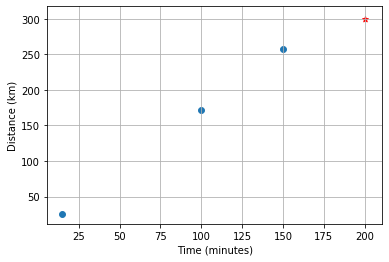
\includegraphics[width=0.7\textwidth]{interp_example1.png}
  \caption{An example of sampling of traveled distances at some time. The red point shows an additional sample taken after the trip velocity has been reduced.}
\end{figure}

Given two samples of the car traveled distance \(s_1\) and \(s_2\) taken at two different times \(t_1\) and \(t_2\) you can linearly interpolate to find your position at different times using the following relations:

\[s = (1 - w)\cdot s_1 + w \cdot s_2\]
where $t$ is a generic time at which we want to know the distance $s$ and \(w = \cfrac{t - t_1}{t_2 - t_1}\).

\subsubsection{Derivation}
The equation of a line for two points
\((t_1, s_1)\) and \((t_2, s_2)\) can be written as:

\[\frac{t - t_1}{t_2 - t_1} = \frac{s - s_1}{s_2 - s_1}\]

Setting \(w = \cfrac{t - t_1}{t_2 - t_1}\) and solving for \(s\) we find the desired solution:

\[(s_2 - s_1)\cdot w = s - s_1~~~\Rightarrow~~~s = (1 - w)\cdot s_1 + w \cdot s_2\]

This formula can also be understood as a weighted average where the weights are inversely related to the distance from the end points to the unknown point ($w_1 = (1 - w) = \cfrac{t_2 - t}{t_2 -t_1}, w_2 = w$), the closer point has more influence than the farther point.

Back to our example, if
\(s_1 = 25.75~\mathrm{km}\;(@t_1 = 15~\mathrm{min})\) and
\(s_2 = 171.7~\mathrm{km}\;(@t_2 = 100~\mathrm{min})\) let's find distance traveled in 1 hour (interpolation):

\begin{tcolorbox}[breakable, size=fbox, boxrule=1pt, pad at break*=1mm,colback=cellbackground, colframe=cellborder]
\begin{Verbatim}[commandchars=\\\{\}]
\PY{n}{s\PYZus{}1} \PY{o}{=} \PY{l+m+mf}{25.75} \PY{c+c1}{\PYZsh{} distance in km}
\PY{n}{t\PYZus{}1} \PY{o}{=} \PY{l+m+mi}{15}    \PY{c+c1}{\PYZsh{} elapsed time in minutes}
\PY{n}{s\PYZus{}2} \PY{o}{=} \PY{l+m+mf}{171.7}
\PY{n}{t\PYZus{}2} \PY{o}{=} \PY{l+m+mi}{100}

\PY{n}{t} \PY{o}{=} \PY{l+m+mi}{60}

\PY{n}{w} \PY{o}{=} \PY{p}{(}\PY{n}{t} \PY{o}{\PYZhy{}} \PY{n}{t\PYZus{}1}\PY{p}{)}\PY{o}{/}\PY{p}{(}\PY{n}{t\PYZus{}2} \PY{o}{\PYZhy{}} \PY{n}{t\PYZus{}1}\PY{p}{)}
\PY{n}{s} \PY{o}{=} \PY{p}{(}\PY{l+m+mi}{1} \PY{o}{\PYZhy{}} \PY{n}{w}\PY{p}{)}\PY{o}{*}\PY{n}{s\PYZus{}1} \PY{o}{+} \PY{n}{w}\PY{o}{*}\PY{n}{s\PYZus{}2}

\PY{n+nb}{print} \PY{p}{(}\PY{l+s+s2}{\PYZdq{}}\PY{l+s+si}{\PYZob{}:.1f\PYZcb{}}\PY{l+s+s2}{ km}\PY{l+s+s2}{\PYZdq{}}\PY{o}{.}\PY{n}{format}\PY{p}{(}\PY{n}{s}\PY{p}{)}\PY{p}{)}

103.0 km
\end{Verbatim}
\end{tcolorbox}

Always interpret critically your results to guess if they make sense or not. In the previous example we certainly expected something between 25.75 and 171.7~km (our range ends) furthermore since we are looking for the distance at a time which is almost halfway the interval, the result will be somehow in the middle or around 98.6~km. This is indeed more or less what we have got.
This simple reasoning should be applied every time you have a result to quickly judge it.

If we believe the relation between our variable stays the same ($f(t)$ still linear), we can use the same formula to \emph{extrapolate} values \emph{outside} our initial sample. For example if we keep the same constant velocity in our trip we could check the distance traveled after 3 hours:

\begin{tcolorbox}[breakable, size=fbox, boxrule=1pt, pad at break*=1mm,colback=cellbackground, colframe=cellborder]
\begin{Verbatim}[commandchars=\\\{\}]
\PY{n}{s\PYZus{}1} \PY{o}{=} \PY{l+m+mf}{25.75} \PY{c+c1}{\PYZsh{} distance in km}
\PY{n}{t\PYZus{}1} \PY{o}{=} \PY{l+m+mi}{15}    \PY{c+c1}{\PYZsh{} elapsed time in minutes}
\PY{n}{s\PYZus{}2} \PY{o}{=} \PY{l+m+mf}{171.7}
\PY{n}{t\PYZus{}2} \PY{o}{=} \PY{l+m+mi}{100}

\PY{n}{t} \PY{o}{=} \PY{l+m+mi}{180}

\PY{n}{w} \PY{o}{=} \PY{p}{(}\PY{n}{t} \PY{o}{\PYZhy{}} \PY{n}{t\PYZus{}1}\PY{p}{)}\PY{o}{/}\PY{p}{(}\PY{n}{t\PYZus{}2} \PY{o}{\PYZhy{}} \PY{n}{t\PYZus{}1}\PY{p}{)}
\PY{n}{s} \PY{o}{=} \PY{p}{(}\PY{l+m+mi}{1} \PY{o}{\PYZhy{}} \PY{n}{w}\PY{p}{)}\PY{o}{*}\PY{n}{s\PYZus{}1} \PY{o}{+} \PY{n}{w}\PY{o}{*}\PY{n}{s\PYZus{}2}

\PY{n+nb}{print} \PY{p}{(}\PY{l+s+s2}{\PYZdq{}}\PY{l+s+si}{\PYZob{}:.1f\PYZcb{}}\PY{l+s+s2}{ km}\PY{l+s+s2}{\PYZdq{}}\PY{o}{.}\PY{n}{format}\PY{p}{(}\PY{n}{s}\PY{p}{)}\PY{p}{)}

309.1 km
\end{Verbatim}
\end{tcolorbox}

\subsection{Log-linear interpolation}\label{log-linear-interpolation}
When the function $f$ that we want to interpolate is an exponential we can fall back to the previous case by a simple variable transformation. 
Assume the following is the relationship between $p$ and $h$, two generic variables:

\[p = \mathrm{exp}(c \cdot h)\]

Applying the logarithm to both sides of the equation gives:

\[s = \mathrm{log}(p) = \mathrm{log}(\mathrm{exp}(c \cdot h)) = c \cdot h\]
so there is linear relation between the new variable $s$ and $h$. At this point we can use the results of the previous section to interpolate for values of $s$, just remember to exponentiate the result to get the correct $p$. In formulas:

\[w = \frac{h - h_1}{h_2 - h_1}\]

\[s = (1 - w)\cdot s_1 + w \cdot s_2\;\;(\mathrm{remember \;now }\;s = \mathrm{log}(p))\]

\[p = \mathrm{exp}(s)\]

Atmospheric pressure decreases with the altitude (i.e.~the highest you flight the lower is the pressure) following an exponential law:

\[p = p_0\cdot e^{-\alpha h}\]
where
\begin{itemize}
\tightlist
\item
  \(h\) is the altitude
\item
  \(p_0\) is the pressure at sea level
\item
  \(\alpha\) is a constant
\end{itemize}

Taking the logarithm of each side of the equation I get a linear relation which can be interpolated as seen before:

\[s = \mathrm{log}(p) = \mathrm{log}(p_0\cdot e^{-\alpha h})\propto - \alpha \cdot h\]

Now assume that we have measured
\(p_1 = 90~\mathrm{kPa}\;(h_1 = 1000~\mathrm{m})\) and
\(p_2 = 40~\mathrm{kPa}\;(h_1 = 7000~\mathrm{m})\) what will be the
atmospheric pressure on top of the Mont Blanc (\(4812~\mathrm{m}\)) ? and on top of Mount Everest (\(8848~\mathrm{m}\)) ?

\begin{tcolorbox}[breakable, size=fbox, boxrule=1pt, pad at break*=1mm,colback=cellbackground, colframe=cellborder]
\begin{Verbatim}[commandchars=\\\{\}]
\PY{c+c1}{\PYZsh{} pressure on top of the Mont Blanc (interpolation)}
\PY{k+kn}{from} \PY{n+nn}{math} \PY{k}{import} \PY{n}{log}\PY{p}{,} \PY{n}{exp}

\PY{c+c1}{\PYZsh{} first we take the logarithm of our measurements to use the linear }
\PY{c+c1}{\PYZsh{} relation to interpolate}
\PY{n}{h\PYZus{}1} \PY{o}{=} \PY{l+m+mi}{1000} \PY{c+c1}{\PYZsh{} height in meters}
\PY{n}{s\PYZus{}1} \PY{o}{=} \PY{n}{log}\PY{p}{(}\PY{l+m+mi}{90}\PY{p}{)} \PY{c+c1}{\PYZsh{} logarithm of the pressure at heigth h1}
\PY{n}{h\PYZus{}2} \PY{o}{=} \PY{l+m+mi}{7000} \PY{c+c1}{\PYZsh{} height in meters}
\PY{n}{s\PYZus{}2} \PY{o}{=} \PY{n}{log}\PY{p}{(}\PY{l+m+mi}{40}\PY{p}{)} \PY{c+c1}{\PYZsh{} logarithm of the pressure at heigth h2}

\PY{n}{h} \PY{o}{=} \PY{l+m+mi}{4812}

\PY{n}{w} \PY{o}{=} \PY{p}{(}\PY{n}{h} \PY{o}{\PYZhy{}} \PY{n}{h\PYZus{}1}\PY{p}{)}\PY{o}{/}\PY{p}{(}\PY{n}{h\PYZus{}2} \PY{o}{\PYZhy{}} \PY{n}{h\PYZus{}1}\PY{p}{)}
\PY{n}{s} \PY{o}{=} \PY{p}{(}\PY{l+m+mi}{1} \PY{o}{\PYZhy{}} \PY{n}{w}\PY{p}{)}\PY{o}{*}\PY{n}{s\PYZus{}1} \PY{o}{+} \PY{n}{w}\PY{o}{*}\PY{n}{s\PYZus{}2}

\PY{n+nb}{print} \PY{p}{(}\PY{l+s+s2}{\PYZdq{}}\PY{l+s+si}{\PYZob{}:.1f\PYZcb{}}\PY{l+s+s2}{ kPa}\PY{l+s+s2}{\PYZdq{}}\PY{o}{.}\PY{n}{format}\PY{p}{(}\PY{n}{exp}\PY{p}{(}\PY{n}{s}\PY{p}{)}\PY{p}{)}\PY{p}{)}

53.8 kPa
\end{Verbatim}
\end{tcolorbox}

\begin{tcolorbox}[breakable, size=fbox, boxrule=1pt, pad at break*=1mm,colback=cellbackground, colframe=cellborder]
\begin{Verbatim}[commandchars=\\\{\}]
\PY{c+c1}{\PYZsh{} pressure on top of the Mount Everest (extrapolation)}
\PY{k+kn}{from} \PY{n+nn}{math} \PY{k}{import} \PY{n}{log}\PY{p}{,} \PY{n}{exp}

\PY{c+c1}{\PYZsh{} first we take the logarithm of our measurements to use the linear }
\PY{c+c1}{\PYZsh{} relation to interpolate}
\PY{n}{h\PYZus{}1} \PY{o}{=} \PY{l+m+mi}{1000} \PY{c+c1}{\PYZsh{} height in meters}
\PY{n}{s\PYZus{}1} \PY{o}{=} \PY{n}{log}\PY{p}{(}\PY{l+m+mi}{90}\PY{p}{)} \PY{c+c1}{\PYZsh{} logarithm of the pressure at heigth h1}
\PY{n}{h\PYZus{}2} \PY{o}{=} \PY{l+m+mi}{7000} \PY{c+c1}{\PYZsh{} height in meters}
\PY{n}{s\PYZus{}2} \PY{o}{=} \PY{n}{log}\PY{p}{(}\PY{l+m+mi}{40}\PY{p}{)} \PY{c+c1}{\PYZsh{} logarithm of the pressure at heigth h2}
\PY{n}{h} \PY{o}{=} \PY{l+m+mi}{8848}

\PY{n}{w} \PY{o}{=} \PY{p}{(}\PY{n}{h} \PY{o}{\PYZhy{}} \PY{n}{h\PYZus{}1}\PY{p}{)}\PY{o}{/}\PY{p}{(}\PY{n}{h\PYZus{}2} \PY{o}{\PYZhy{}} \PY{n}{h\PYZus{}1}\PY{p}{)}
\PY{n}{s} \PY{o}{=} \PY{p}{(}\PY{l+m+mi}{1} \PY{o}{\PYZhy{}} \PY{n}{w}\PY{p}{)}\PY{o}{*}\PY{n}{s\PYZus{}1} \PY{o}{+} \PY{n}{w}\PY{o}{*}\PY{n}{s\PYZus{}2}

\PY{n+nb}{print} \PY{p}{(}\PY{l+s+s2}{\PYZdq{}}\PY{l+s+si}{\PYZob{}:.1f\PYZcb{}}\PY{l+s+s2}{ kPa}\PY{l+s+s2}{\PYZdq{}}\PY{o}{.}\PY{n}{format}\PY{p}{(}\PY{n}{exp}\PY{p}{(}\PY{n}{s}\PY{p}{)}\PY{p}{)}\PY{p}{)}

31.2 kPa
\end{Verbatim}
\end{tcolorbox}

\begin{figure}
\centering
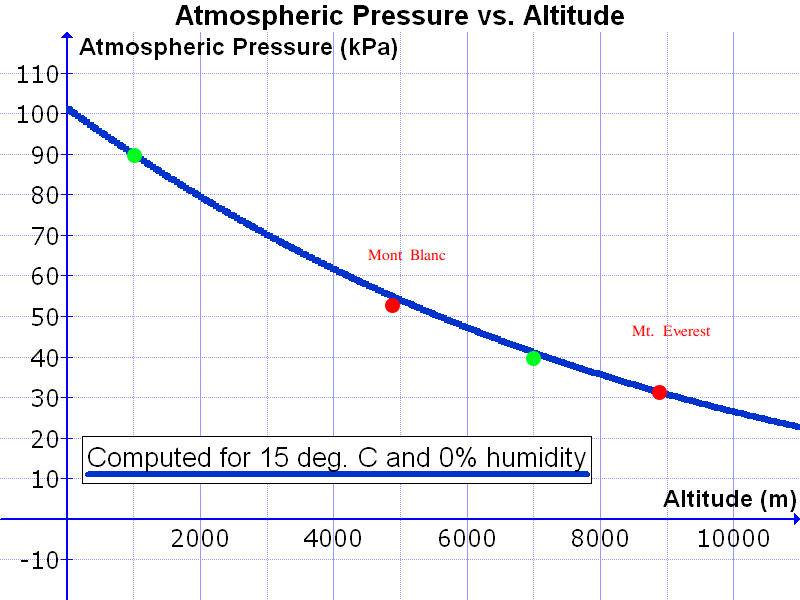
\includegraphics[width=0.7\linewidth]{Atmospheric_Pressure_vs._Altitude.png}
\caption{Atmospheric pressure versus altitude (Wikipedia). Green points
represent our measurements, red points represent
interpolation/extrapolation.}
\end{figure}

\subsection{Limitations of Interpolation}
Interpolation is just an approximation and works well when either the function $f$ is linear or we are trying to interpolate between two points that are close enough to believe that $f$ is almost linear in that interval.

It can be easily demonstrated that the linear approximation between two points of a given function $f(x)$ gets worse with the second derivative of the function that is approximated ($f''(x)$). This is intuitively correct: the "curvier" the function is, the worse the approximation made with simple linear interpolation becomes, see Fig.~\ref{fig:sine_interp}.

\begin{figure}
  \centering
  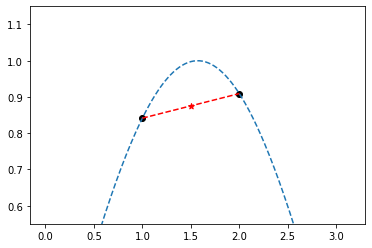
\includegraphics[width=0.7\textwidth]{wrong_interp.png}
  \caption{Trying to approximate a sine function with a line is clearly not going to work unless the interpolation interval is very small.}
  \label{fig:sine_interp}
\end{figure}

To improve the approximation accuracy with complicated curves a polynomial of higher order can be used ($𝑝(𝑥)=𝑎_0 + 𝑎_1 𝑥+ 𝑎_2 𝑥^2+\cdots$), for example in the evaluation of the natural logarithm and trigonometric functions. It has to be clear however that going to higher degrees does not always help (for those interested \href{https://en.wikipedia.org/wiki/Runge%27s_phenomenon}{see Runge's phenomenon}).

\section{Discount curve interpolation}\label{discount-curve-interpolation}

Finally we can come back to finance. Since discount factors are derived from a discrete set of dates we may need to find the factor at some different date and clearly we can use interpolation to do it.
Now we will see how to implement a \texttt{python} function which interpolates some given discount factors.
Needed data:

\begin{itemize}
\tightlist
\item a list of pillars dates specifying the value dates of the given discount factors, \(t_0,...,t_{n-1}\);
\item a list of given discount factors, \(D(t_0),...,D(t_{n-1})\);
\item a pricing date (`today' date) which corresponds to \(t=0\).
\end{itemize}

The input argument to the function will be the value date at which we want to interpolate the discount factor. Since the discount factor can be expressed as \(D=e^{-r(T-t)}\) the function will use a log-linear interpolation to return the value at a date not included in the given pillars.
More technically we can say that we are doing a linear interpolation over time in the log space:

\[d(t_i):=\mathrm{ln}(D(t_i))\]

\[d(t) = (1-w)d(t_i) + wd(t_{i+1});\;\;\;w=\frac{t-t_i}{t_{i+1}-t_i}\]

\[D(t) = \mathrm{exp}(d(t))\]
where again \(i\) is such that \(t_i \le t \le t_{i+1}\)

This time instead of reinventing the wheel and performing the interpolation with our own code, we'll use the function \texttt{interp} provided by the module \texttt{numpy}; this function linearly interpolates between the provided points to estimate the value of $f$ at some "new" $x$.
Say we want to interpolate the points at $x = 2.5$ given the following values:

\begin{tcolorbox}[breakable, size=fbox, boxrule=1pt, pad at break*=1mm,colback=cellbackground, colframe=cellborder]
\begin{Verbatim}[commandchars=\\\{\}]
\PY{k+kn}{import} \PY{n+nn}{numpy} \PY{k}{as} \PY{n+nn}{np}

\PY{n}{xp} \PY{o}{=} \PY{p}{[}\PY{l+m+mi}{0}\PY{p}{,} \PY{l+m+mi}{1}\PY{p}{,} \PY{l+m+mi}{5}\PY{p}{]}
\PY{n}{fp} \PY{o}{=} \PY{p}{[}\PY{l+m+mi}{0}\PY{p}{,} \PY{l+m+mi}{2}\PY{p}{,} \PY{l+m+mi}{4}\PY{p}{]}
\PY{n}{np}\PY{o}{.}\PY{n}{interp}\PY{p}{(}\PY{l+m+mf}{2.5}\PY{p}{,} \PY{n}{xp}\PY{p}{,} \PY{n}{fp}\PY{p}{)}

2.75
\end{Verbatim}
\end{tcolorbox}

Assume we have three discount factors instead:
\begin{tcolorbox}[breakable, size=fbox, boxrule=1pt, pad at break*=1mm,colback=cellbackground, colframe=cellborder]
\begin{Verbatim}[commandchars=\\\{\}]
\PY{c+c1}{\PYZsh{} import modules and objects that we need}
\PY{k+kn}{from} \PY{n+nn}{datetime} \PY{k}{import} \PY{n}{date}
\PY{k+kn}{import} \PY{n+nn}{numpy}\PY{o}{,} \PY{n+nn}{math}
\PY{k+kn}{from} \PY{n+nn}{matplotlib} \PY{k}{import} \PY{n}{pyplot} \PY{k}{as} \PY{n}{plt}
\PY{k+kn}{import} \PY{n+nn}{matplotlib}\PY{n+nn}{.}\PY{n+nn}{dates} \PY{k}{as} \PY{n+nn}{mdates} 
\PY{c+c1}{\PYZsh{} with this notation we tell python to use mdates as an alias }
\PY{c+c1}{\PYZsh{} for matplotlib.dates}

\PY{c+c1}{\PYZsh{} define the input data}
\PY{n}{today\PYZus{}date} \PY{o}{=} \PY{n}{date}\PY{p}{(}\PY{l+m+mi}{2019}\PY{p}{,} \PY{l+m+mi}{10}\PY{p}{,} \PY{l+m+mi}{1}\PY{p}{)}

\PY{n}{pillar\PYZus{}dates} \PY{o}{=} \PY{p}{[}\PY{n}{date}\PY{p}{(}\PY{l+m+mi}{2019}\PY{p}{,} \PY{l+m+mi}{10}\PY{p}{,} \PY{l+m+mi}{1}\PY{p}{)}\PY{p}{,} \PY{n}{date}\PY{p}{(}\PY{l+m+mi}{2020}\PY{p}{,} \PY{l+m+mi}{10}\PY{p}{,} \PY{l+m+mi}{1}\PY{p}{)}\PY{p}{,} \PY{n}{date}\PY{p}{(}\PY{l+m+mi}{2021}\PY{p}{,} \PY{l+m+mi}{10}\PY{p}{,} \PY{l+m+mi}{1}\PY{p}{)}\PY{p}{]}
\PY{n}{discount\PYZus{}factors} \PY{o}{=} \PY{p}{[}\PY{l+m+mf}{1.0}\PY{p}{,} \PY{l+m+mf}{0.97}\PY{p}{,} \PY{l+m+mf}{0.72}\PY{p}{]}
\end{Verbatim}
\end{tcolorbox}
    
Let's see what this fake discount curve looks like when plotted on a graph:

\begin{tcolorbox}[breakable, size=fbox, boxrule=1pt, pad at break*=1mm,colback=cellbackground, colframe=cellborder]
\begin{Verbatim}[commandchars=\\\{\}]
\PY{n}{plt}\PY{o}{.}\PY{n}{plot}\PY{p}{(}\PY{n}{pillar\PYZus{}dates}\PY{p}{,} \PY{n}{discount\PYZus{}factors}\PY{p}{,} \PY{n}{marker}\PY{o}{=}\PY{l+s+s1}{\PYZsq{}}\PY{l+s+s1}{o}\PY{l+s+s1}{\PYZsq{}}\PY{p}{)}
\PY{n}{plt}\PY{o}{.}\PY{n}{gca}\PY{p}{(}\PY{p}{)}\PY{o}{.}\PY{n}{xaxis}\PY{o}{.}\PY{n}{set\PYZus{}major\PYZus{}formatter}\PY{p}{(}\PY{n}{mdates}\PY{o}{.}\PY{n}{DateFormatter}\PY{p}{(}\PY{l+s+s1}{\PYZsq{}}\PY{l+s+s1}{\PYZpc{}}\PY{l+s+s1}{m/}\PY{l+s+si}{\PYZpc{}d}\PY{l+s+s1}{/}\PY{l+s+s1}{\PYZpc{}}\PY{l+s+s1}{Y}\PY{l+s+s1}{\PYZsq{}}\PY{p}{)}\PY{p}{)}
\PY{n}{plt}\PY{o}{.}\PY{n}{gca}\PY{p}{(}\PY{p}{)}\PY{o}{.}\PY{n}{xaxis}\PY{o}{.}\PY{n}{set\PYZus{}major\PYZus{}locator}\PY{p}{(}\PY{n}{mdates}\PY{o}{.}\PY{n}{YearLocator}\PY{p}{(}\PY{p}{)}\PY{p}{)}
\PY{n}{plt}\PY{o}{.}\PY{n}{grid}\PY{p}{(}\PY{k+kc}{True}\PY{p}{)}
\PY{n}{plt}\PY{o}{.}\PY{n}{show}\PY{p}{(}\PY{p}{)}
\end{Verbatim}
\end{tcolorbox}
\vfill
\begin{figure}[h]
  \centering
  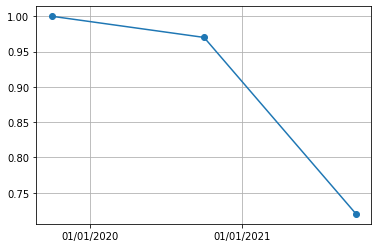
\includegraphics[width=0.7\textwidth]{lecture_3_10_0.png}
\end{figure}
    
Since it is a computation that from now on we need to perform quite often it is convenient to write a function that compute the discount factor at arbitrary dates.

\begin{tcolorbox}[breakable, size=fbox, boxrule=1pt, pad at break*=1mm,colback=cellbackground, colframe=cellborder]
\begin{Verbatim}[commandchars=\\\{\}]
\PY{c+c1}{\PYZsh{} define the df function}
\PY{k}{def} \PY{n+nf}{df}\PY{p}{(}\PY{n}{d, pillar_dates, discount_factors}\PY{p}{)}\PY{p}{:}
    \PY{c+c1}{\PYZsh{} first thing we need to do is to apply the logarithm function}
    \PY{c+c1}{\PYZsh{} to the discount factors since we are doing log-linear and}
    \PY{c+c1}{\PYZsh{} not just linear interpolation}
    \PY{n}{log\PYZus{}discount\PYZus{}factors} \PY{o}{=} \PY{p}{[}\PY{p}{]}
    \PY{k}{for} \PY{n}{discount\PYZus{}factor} \PY{o+ow}{in} \PY{n}{discount\PYZus{}factors}\PY{p}{:}
        \PY{n}{log\PYZus{}discount\PYZus{}factors}\PY{o}{.}\PY{n}{append}\PY{p}{(}\PY{n}{math}\PY{o}{.}\PY{n}{log}\PY{p}{(}\PY{n}{discount\PYZus{}factor}\PY{p}{)}\PY{p}{)}
    
    \PY{c+c1}{\PYZsh{} perform the linear interpolation of the log discount factors}
    \PY{n}{interpolated\PYZus{}log\PYZus{}discount\PYZus{}factor} \PY{o}{=} \PYZbs{}
        \PY{n}{numpy}\PY{o}{.}\PY{n}{interp}\PY{p}{(}\PY{n}{d}\PY{p}{,} \PY{n}{pillar\PYZus{}dates}\PY{p}{,} \PY{n}{log\PYZus{}discount\PYZus{}factors}\PY{p}{)}
    
    \PY{c+c1}{\PYZsh{} return the interpolated discount factor}
    \PY{k}{return} \PY{n}{math}\PY{o}{.}\PY{n}{exp}\PY{p}{(}\PY{n}{interpolated\PYZus{}log\PYZus{}discount\PYZus{}factor}\PY{p}{)}
\end{Verbatim}
\end{tcolorbox}

This is almost OK, \textbf{but it won't work} because \texttt{numpy.interp} only accepts numbers or a list of numbers as argument i.e.~it doesn't automatically convert or interpret dates as numbers so doesn't know how to interpolate them. So we need to do the conversion ourselves before passing the dates into the interpolation function.
The following updated version of our function converts the pillar dates into ``pillar days'' i.e. each date is replaced by the number of days today ($t_0$):

\begin{tcolorbox}[breakable, size=fbox, boxrule=1pt, pad at break*=1mm,colback=cellbackground, colframe=cellborder]
\begin{Verbatim}[commandchars=\\\{\}]
\PY{k}{def} \PY{n+nf}{df}\PY{p}{(}\PY{n}{d, today_date, pillar_dates, discount_factors}\PY{p}{)}\PY{p}{:}
    \PY{c+c1}{\PYZsh{} first thing we need to do is to apply the logarithm function}
    \PY{c+c1}{\PYZsh{} to the discount factors since we are doing log-linear and}
    \PY{c+c1}{\PYZsh{} not just linear interpolation}
    \PY{n}{log\PYZus{}discount\PYZus{}factors} \PY{o}{=} \PY{p}{[}\PY{p}{]}
    \PY{k}{for} \PY{n}{discount\PYZus{}factor} \PY{o+ow}{in} \PY{n}{discount\PYZus{}factors}\PY{p}{:}
        \PY{n}{log\PYZus{}discount\PYZus{}factors}\PY{o}{.}\PY{n}{append}\PY{p}{(}\PY{n}{math}\PY{o}{.}\PY{n}{log}\PY{p}{(}\PY{n}{discount\PYZus{}factor}\PY{p}{)}\PY{p}{)}
    
    \PY{c+c1}{\PYZsh{} convert the pillar dates to pillar \PYZsq{}days\PYZsq{}}
    \PY{c+c1}{\PYZsh{} i.e. number of days from today}
    \PY{c+c1}{\PYZsh{} to write shorter code we can use this NEW notation}
    \PY{c+c1}{\PYZsh{} which condenses for and list creation in one line}
    \PY{n}{pillar\PYZus{}days} \PY{o}{=} \PYZbs{}
        \PY{p}{[}\PY{p}{(}\PY{n}{pillar\PYZus{}date} \PY{o}{\PYZhy{}} \PY{n}{today\PYZus{}date}\PY{p}{)}\PY{o}{.}\PY{n}{days} \PY{k}{for} \PY{n}{pillar\PYZus{}date} \PY{o+ow}{in} \PY{n}{pillar\PYZus{}dates}\PY{p}{]}
    
    \PY{c+c1}{\PYZsh{} obviously we need to do the same to the value date}
    \PY{c+c1}{\PYZsh{} argument of the df function}
    \PY{n}{d\PYZus{}days} \PY{o}{=} \PY{p}{(}\PY{n}{d} \PY{o}{\PYZhy{}} \PY{n}{today\PYZus{}date}\PY{p}{)}\PY{o}{.}\PY{n}{days}
    
    \PY{c+c1}{\PYZsh{} perform the linear interpolation of the log discount factors}
    \PY{n}{interpolated\PYZus{}log\PYZus{}discount\PYZus{}factor} \PY{o}{=} \PYZbs{}
        \PY{n}{numpy}\PY{o}{.}\PY{n}{interp}\PY{p}{(}\PY{n}{d\PYZus{}days}\PY{p}{,} \PY{n}{pillar\PYZus{}days}\PY{p}{,} \PY{n}{log\PYZus{}discount\PYZus{}factors}\PY{p}{)}
    
    \PY{c+c1}{\PYZsh{} return the interpolated discount factor}
    \PY{k}{return} \PY{n}{math}\PY{o}{.}\PY{n}{exp}\PY{p}{(}\PY{n}{interpolated\PYZus{}log\PYZus{}discount\PYZus{}factor}\PY{p}{)}
\end{Verbatim}
\end{tcolorbox}

Now we can use the \texttt{df} function to get discount factors on value dates between the given pillar dates:

\begin{tcolorbox}[breakable, size=fbox, boxrule=1pt, pad at break*=1mm,colback=cellbackground, colframe=cellborder]
\begin{Verbatim}[commandchars=\\\{\}]
\PY{n}{d0} \PY{o}{=} \PY{n}{date}\PY{p}{(}\PY{l+m+mi}{2020}\PY{p}{,} \PY{l+m+mi}{1}\PY{p}{,} \PY{l+m+mi}{1}\PY{p}{)}
\PY{n}{df0} \PY{o}{=} \PY{n}{df}\PY{p}{(}\PY{n}{d0, today_date, pillar_dates, discount_factors}\PY{p}{)}
\PY{n+nb}{print} \PY{p}{(}\PY{n}{df0}\PY{p}{)}

0.9923728228571693
\end{Verbatim}
\end{tcolorbox}

\begin{tcolorbox}[breakable, size=fbox, boxrule=1pt, pad at break*=1mm,colback=cellbackground, colframe=cellborder]
\begin{Verbatim}[commandchars=\\\{\}]
\PY{n}{d1} \PY{o}{=} \PY{n}{date}\PY{p}{(}\PY{l+m+mi}{2021}\PY{p}{,} \PY{l+m+mi}{1}\PY{p}{,} \PY{l+m+mi}{1}\PY{p}{)}
\PY{n}{df1} \PY{o}{=} \PY{n}{df}\PY{p}{(}\PY{n}{d1, today_date, pillar_dates, discount_factors}\PY{p}{)}
\PY{n+nb}{print} \PY{p}{(}\PY{n}{df1}\PY{p}{)}

0.8997999273630835
\end{Verbatim}
\end{tcolorbox}

Another very useful way to check the correctness of a result is by plotting data, so let's see what these look like when plotted on a semi-log graph and if they make sense:
    
\begin{tcolorbox}[breakable, size=fbox, boxrule=1pt, pad at break*=1mm,colback=cellbackground, colframe=cellborder]
\begin{Verbatim}[commandchars=\\\{\}]
\PY{k+kn}{from} \PY{n+nn}{matplotlib} \PY{k}{import} \PY{n}{pyplot} \PY{k}{as} \PY{n}{plt}
\PY{k+kn}{import} \PY{n+nn}{matplotlib}\PY{n+nn}{.}\PY{n+nn}{dates} \PY{k}{as} \PY{n+nn}{mdates}

\PY{n}{plt}\PY{o}{.}\PY{n}{semilogy}\PY{p}{(}\PY{n}{pillar\PYZus{}dates}\PY{p}{,} \PY{n}{discount\PYZus{}factors}\PY{p}{,} \PY{n}{marker}\PY{o}{=}\PY{l+s+s1}{\PYZsq{}}\PY{l+s+s1}{o}\PY{l+s+s1}{\PYZsq{}}\PY{p}{)}
\PY{n}{plt}\PY{o}{.}\PY{n}{semilogy}\PY{p}{(}\PY{n}{d0}\PY{p}{,}\PY{n}{df0} \PY{p}{,} \PY{n}{marker}\PY{o}{=}\PY{l+s+s1}{\PYZsq{}}\PY{l+s+s1}{X}\PY{l+s+s1}{\PYZsq{}}\PY{p}{)}
\PY{n}{plt}\PY{o}{.}\PY{n}{semilogy}\PY{p}{(}\PY{n}{d1}\PY{p}{,}\PY{n}{df1} \PY{p}{,} \PY{n}{marker}\PY{o}{=}\PY{l+s+s1}{\PYZsq{}}\PY{l+s+s1}{X}\PY{l+s+s1}{\PYZsq{}}\PY{p}{)}
\PY{n}{plt}\PY{o}{.}\PY{n}{gca}\PY{p}{(}\PY{p}{)}\PY{o}{.}\PY{n}{xaxis}\PY{o}{.}\PY{n}{set\PYZus{}major\PYZus{}formatter}\PY{p}{(}\PY{n}{mdates}\PY{o}{.}\PY{n}{DateFormatter}\PY{p}{(}\PY{l+s+s1}{\PYZsq{}}\PY{l+s+s1}{\PYZpc{}}\PY{l+s+s1}{m/}\PY{l+s+si}{\PYZpc{}d}\PY{l+s+s1}{/}\PY{l+s+s1}{\PYZpc{}}\PY{l+s+s1}{Y}\PY{l+s+s1}{\PYZsq{}}\PY{p}{)}\PY{p}{)}
\PY{n}{plt}\PY{o}{.}\PY{n}{gca}\PY{p}{(}\PY{p}{)}\PY{o}{.}\PY{n}{xaxis}\PY{o}{.}\PY{n}{set\PYZus{}major\PYZus{}locator}\PY{p}{(}\PY{n}{mdates}\PY{o}{.}\PY{n}{YearLocator}\PY{p}{(}\PY{p}{)}\PY{p}{)}
\PY{n}{plt}\PY{o}{.}\PY{n}{grid}\PY{p}{(}\PY{k+kc}{True}\PY{p}{)}
\PY{n}{plt}\PY{o}{.}\PY{n}{show}\PY{p}{(}\PY{p}{)}
\end{Verbatim}
\end{tcolorbox}
\vfill
\begin{figure}[h]
  \centering
  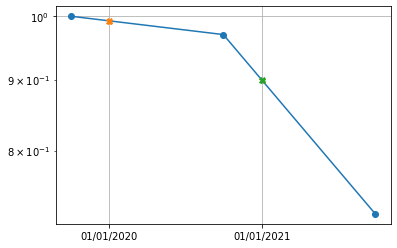
\includegraphics[width=0.7\textwidth]{lecture_3_15_0.png}
\end{figure}

Let's see what these look like when plotted on a linear graph instead:
    
\begin{tcolorbox}[breakable, size=fbox, boxrule=1pt, pad at break*=1mm,colback=cellbackground, colframe=cellborder]
\begin{Verbatim}[commandchars=\\\{\}]
\PY{k+kn}{from} \PY{n+nn}{matplotlib} \PY{k}{import} \PY{n}{pyplot} \PY{k}{as} \PY{n}{plt}
\PY{k+kn}{import} \PY{n+nn}{matplotlib}\PY{n+nn}{.}\PY{n+nn}{dates} \PY{k}{as} \PY{n+nn}{mdates}
\PY{n}{plt}\PY{o}{.}\PY{n}{plot}\PY{p}{(}\PY{n}{pillar\PYZus{}dates}\PY{p}{,} \PY{n}{discount\PYZus{}factors}\PY{p}{,} \PY{n}{marker}\PY{o}{=}\PY{l+s+s1}{\PYZsq{}}\PY{l+s+s1}{o}\PY{l+s+s1}{\PYZsq{}}\PY{p}{)}
\PY{n}{plt}\PY{o}{.}\PY{n}{plot}\PY{p}{(}\PY{n}{d0}\PY{p}{,}\PY{n}{df0} \PY{p}{,} \PY{n}{marker}\PY{o}{=}\PY{l+s+s1}{\PYZsq{}}\PY{l+s+s1}{X}\PY{l+s+s1}{\PYZsq{}}\PY{p}{)}
\PY{n}{plt}\PY{o}{.}\PY{n}{plot}\PY{p}{(}\PY{n}{d1}\PY{p}{,}\PY{n}{df1} \PY{p}{,} \PY{n}{marker}\PY{o}{=}\PY{l+s+s1}{\PYZsq{}}\PY{l+s+s1}{X}\PY{l+s+s1}{\PYZsq{}}\PY{p}{)}
\PY{n}{plt}\PY{o}{.}\PY{n}{gca}\PY{p}{(}\PY{p}{)}\PY{o}{.}\PY{n}{xaxis}\PY{o}{.}\PY{n}{set\PYZus{}major\PYZus{}formatter}\PY{p}{(}\PY{n}{mdates}\PY{o}{.}\PY{n}{DateFormatter}\PY{p}{(}\PY{l+s+s1}{\PYZsq{}}\PY{l+s+s1}{\PYZpc{}}\PY{l+s+s1}{m/}\PY{l+s+si}{\PYZpc{}d}\PY{l+s+s1}{/}\PY{l+s+s1}{\PYZpc{}}\PY{l+s+s1}{Y}\PY{l+s+s1}{\PYZsq{}}\PY{p}{)}\PY{p}{)}
\PY{n}{plt}\PY{o}{.}\PY{n}{gca}\PY{p}{(}\PY{p}{)}\PY{o}{.}\PY{n}{xaxis}\PY{o}{.}\PY{n}{set\PYZus{}major\PYZus{}locator}\PY{p}{(}\PY{n}{mdates}\PY{o}{.}\PY{n}{YearLocator}\PY{p}{(}\PY{p}{)}\PY{p}{)}
\PY{n}{plt}\PY{o}{.}\PY{n}{grid}\PY{p}{(}\PY{k+kc}{True}\PY{p}{)}
\PY{n}{plt}\PY{o}{.}\PY{n}{show}\PY{p}{(}\PY{p}{)}
\end{Verbatim}
\end{tcolorbox}
\vfill
\begin{figure}[h]
  \centering
  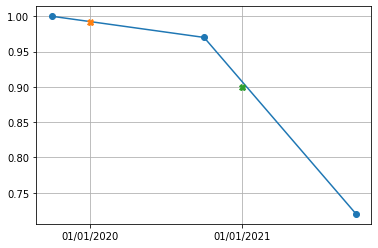
\includegraphics[width=0.7\textwidth]{lecture_3_16_0.png}
\end{figure}

Discrepancies in the linear plot are most likely due to rounding.

\section{Forward Rates}\label{calculating-forward-rates}

A forward rate is an interest rate applicable to a financial transaction that will take place in the future. Forward rates are calculated from the spot rate by exploiting the no arbitrage condition which states that investing at rate \(r_1\) for the period \((0, T_1)\) and then \emph{re-investing} at rate \(r_{1,2}\) for the time period \((T_1, T_2)\) is equivalent to invest at rate \(r_2\) for the full time period \((0, T_2)\). Essentially two investors shouldn't be able to earn money from arbitraging between different interest periods. That said:

\[(1+r_1 T_1)(1+r_{1,2}(T_2 - T_1)) = 1 + r_2 T_2\]

Solving for \(r_{1,2}\) leads to

\[F(T_1, T_2) = r_{1,2} = \frac{1}{T_2-T_1}\Big(\frac{D(T_1)}{D(T_2)} - 1 \Big)~~~~\textrm{(where $D{(T_i)}=\frac{1}{1+r_iT_{i}}$)}\]

\begin{tcolorbox}[breakable, size=fbox, boxrule=1pt, pad at break*=1mm,colback=cellbackground, colframe=cellborder]
\begin{Verbatim}[commandchars=\\\{\}]
\PY{k+kn}{from} \PY{n+nn}{datetime} \PY{k}{import} \PY{n}{date}
\PY{k+kn}{import} \PY{n+nn}{numpy}\PY{o}{,} \PY{n+nn}{math}

\PY{n}{today\PYZus{}date} \PY{o}{=} \PY{n}{date} \PY{p}{(}\PY{l+m+mi}{2019}\PY{p}{,} \PY{l+m+mi}{1}\PY{p}{,} \PY{l+m+mi}{1}\PY{p}{)}

\PY{n}{pillar\PYZus{}dates} \PY{o}{=} \PY{p}{[}\PY{n}{date}\PY{p}{(}\PY{l+m+mi}{2019} \PY{p}{,} \PY{l+m+mi}{1} \PY{p}{,}\PY{l+m+mi}{1}\PY{p}{)}\PY{p}{,} 
                \PY{n}{date}\PY{p}{(}\PY{l+m+mi}{2020}\PY{p}{,} \PY{l+m+mi}{1}\PY{p}{,} \PY{l+m+mi}{1}\PY{p}{)}\PY{p}{,} 
                \PY{n}{date}\PY{p}{(}\PY{l+m+mi}{2021}\PY{p}{,} \PY{l+m+mi}{10} \PY{p}{,}\PY{l+m+mi}{1}\PY{p}{)}\PY{p}{]}
\PY{n}{discount\PYZus{}factors} \PY{o}{=} \PY{p}{[}\PY{l+m+mf}{1.0}\PY{p}{,} \PY{l+m+mf}{0.97}\PY{p}{,} \PY{l+m+mf}{0.72}\PY{p}{]}

\PY{k}{def} \PY{n+nf}{forward\PYZus{}rate}\PY{p}{(}\PY{n}{t1}\PY{p}{,} \PY{n}{t2, today_date, pillar_dates, discount_factors}\PY{p}{)}\PY{p}{:}
    \PY{k}{return} \PY{l+m+mf}{365.0}\PY{o}{/}\PY{p}{(}\PY{n}{t2}\PY{o}{\PYZhy{}}\PY{n}{t1}\PY{p}{)}\PY{o}{.}\PY{n}{days} \PY{o}{*}
        \PY{p}{(}\PY{n}{df}\PY{p}{(}\PY{n}{t1, today_date, pillar_dates, discount_factors}\PY{p}{)} \PY{o}{/}
        \PY{n}{df}\PY{p}{(}\PY{n}{t2, today_date, pillar_dates, discount_factors}\PY{p}{)} \PY{o}{\PYZhy{}} \PY{l+m+mi}{1}\PY{p}{)}

\PY{n}{forward\PYZus{}rate}\PY{p}{(}\PY{n}{date}\PY{p}{(}\PY{l+m+mi}{2019}\PY{p}{,} \PY{l+m+mi}{2}\PY{p}{,} \PY{l+m+mi}{1}\PY{p}{)}\PY{p}{,} \PY{n}{date}\PY{p}{(}\PY{l+m+mi}{2019}\PY{p}{,} \PY{l+m+mi}{8}\PY{p}{,} \PY{l+m+mi}{1}\PY{p}{),}
             \PY{p}{today_date, pillar_dates, discount_factors}\PY{p}{)}
\end{Verbatim}
\end{tcolorbox}

\subsection{2008 Financial Crisis}\label{financial-crisis}

Looking at the historical series of the Euribor (6M) rate versus the Eonia Overnight Indexed Swap (OIS-6M) rate over the time interval 2006-2011 it becomes apparent how before August 2007 the two rates display strictly overlapping trends differing of no more than 6 bps.

\begin{figure}[h]
\centering
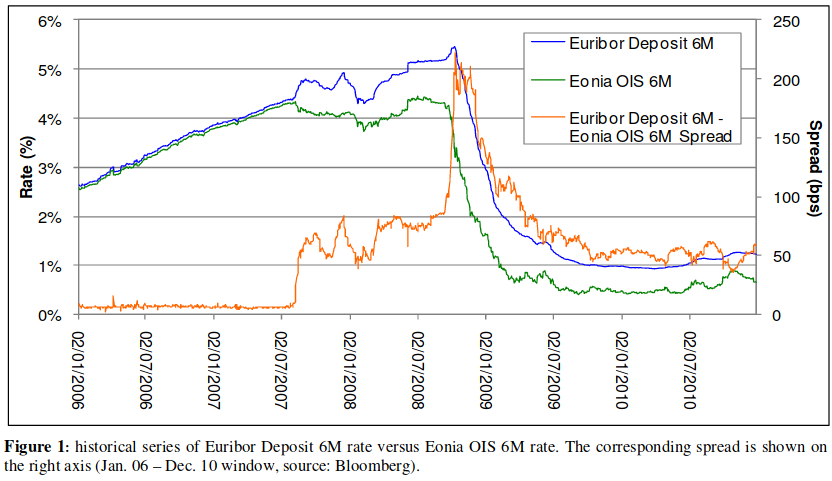
\includegraphics[width=0.7\linewidth]{credit_crunch.png}
\end{figure}

In August 2007 however we observe a sudden increase of the Euribor rate and a simultaneous decrease of the OIS rate that leads to the explosion of the corresponding basis spread, touching the peak of 222 bps in October 2008, when Lehman Brothers filed for bankruptcy. Successively the basis has sensibly reduced and stabilized between 40 bps and 60 bps (notice that the pre-crisis level has never been recovered). The same effect is observed for other similar couples of series, e.g.~Euribor 3M vs OIS 3M.

The reason of the abrupt divergence between the Euribor and OIS rates can be explained by considering both the monetary policy decisions adopted by international authorities in response to the financial turmoil, and the impact of the credit crunch on both credit and liquidity risk perception of the market, coupled with the different financial meaning and dynamics of these rates.

\begin{itemize}
\tightlist
\item
  The Euribor rate is the reference rate for over-the-counter (OTC)
  transactions in the Euro area. It is defined as the rate at which
  Euro inter-bank deposits are being offered within the EMU zone by one
  prime bank to another at 11:00 a.m. Brussels time. The rate fixings
  for a strip of 15 maturities (from one day to one year) are
  constructed as the average of the rates submitted (excluding the
  highest and lowest 15\% tails) by a panel of 42 banks, selected
  among the EU banks with the highest volume of business in the Euro
  zone money markets, plus some large international bank from non-EU
  countries with important euro zone operations. \emph{Thus, Euribor
  rates reflect the average cost of funding of banks in the inter bank
  market at each given maturity. During the crisis the solvency and
  solidity of the whole financial sector was brought into question and
  the credit and liquidity risk and uremia associated to inter-bank
  counter-parties sharply increased.} The Euribor rates immediately
  reflected these dynamics and raise to their highest values over more
  than 10 years. As seen in the plot above, the Euribor 6M rate suddenly
  increased on August 2007 and reached 5.49\% on 10th October 2008.
\item
  The Eonia rate is the reference rate for overnight OTC transactions in
  the Euro area. It is constructed as the average rate of the overnight
  transactions (one day maturity deposits) executed during a given
  business day by a panel of banks on the inter-bank money market,
  weighted with the corresponding transaction volumes. \emph{The Eonia
  Contribution Panel coincides with the Euribor Contribution Panel, thus
  Eonia rate includes information on the short term (overnight)
  liquidity expectations of banks in the Euro money market. It is also
  used by the European Central Bank (ECB) as a method of effecting and
  observing the transmission of its monetary policy actions. During the
  crisis the central banks were mainly concerned about stabilizing the
  level of liquidity in the market, thus they reduced the level of the
  official rates.} Furthermore, the daily tenor of the Eonia rate makes
  negligible the credit and liquidity risks reflected on it: for this
  reason the OIS rates are considered the best proxies available in the
  market for the risk-free rate.
\end{itemize}

As a practical result of the divergence of the two indices, after the 2008 financial crisis, it is not possible anymore to use a single discount curve to correctly price forward rates of all tenors. For example, if we want to calculate the net present value of a forward 6-month Libor coupon, we need to simultaneously use two different discount curves:

\begin{itemize}
\tightlist
\item the 6-month Libor curve for determining the forward rate;
\item the EONIA curve for discounting the expected cash flow.
\end{itemize}

Our financial library will have to implement the following calculation:

\[\mathrm{NPV} = D_{\mathrm{EONIA}}(T_1) \times \frac{1}{T_2-T_1}\Big(\frac{D_{\mathrm{LIBOR}}(T_1)}{D_{\mathrm{LIBOR}}(T_2)} - 1 \Big)\]
and this will asked to be done in the exercises relative to this chapter.

To exploit the Object Oriented capabilities we will implement a \texttt{DiscountCurve} class, below a skeleton class to give you an idea of how could be this new class.
\begin{Shaded}
\begin{Highlighting}[]
\CommentTok{# here goes import statement of the needed modules}
\ImportTok{import}\NormalTok{ ABCD}
\ImportTok{from}\NormalTok{ XYZ }\ImportTok{import}\NormalTok{ xyz}

\CommentTok{# usually classes have CamelCase naming convention}
\KeywordTok{class}\NormalTok{ DiscountCurve:}

    \CommentTok{# the special __init__ method defines }
    \CommentTok{# how to construct instances of the class}
    \CommentTok{# so you need to identify the attributes you need to store }
    \CommentTok{# in the class defining a discount curve}
    \KeywordTok{def} \FunctionTok{__init__}\NormalTok{(}\VariableTok{self}\NormalTok{, ...):}

    \CommentTok{# then we want to add a method to compute the discount}
    \CommentTok{# factor at an arbitrary value date }
    \CommentTok{# using the data stored in the instance}
    \KeywordTok{def}\NormalTok{ df(}\VariableTok{self}\NormalTok{, param1, param2, ...):}
      \CommentTok{# the implementation can follow what we did in the }
      \CommentTok{# function we wrote last week but this time has to }
      \CommentTok{# use the class attributes}
      
    \CommentTok{# finally we want a method to calculates the forward rate }
    \CommentTok{# based on the discount curve data stored in the instance}
    \KeywordTok{def}\NormalTok{ forward_rate(}\VariableTok{self}\NormalTok{, param1, param2, ...):}
        \CommentTok{# here of course we can use the df method }
        \CommentTok{# implemented above to calculate the forward rate}
\end{Highlighting}
\end{Shaded}

\clearpage
\chapter{Swaps and Bootstrapping}\label{swaps-and-bootstrapping---practical-lesson-5}

In this Chapter the Overnight Index Swap contract is reviewed and new class to represent it will be added to our financial module. Beside financial arguments another very important mathematical technique is introduced: the \emph{bootstrapping}.

\section{Payment Dates Generator}
Before going to describe the Overnight Index Swap we need to develop a tool which helps us to generate list of dates (e.g. payment dates), a task that we will need to do often from now on. 
The function we are writing will go in \texttt{finmarkets} module and will be used by the classes describing various kind of contracts (this is essentially the function that was required in Ex. 3.5).

\begin{tcolorbox}[size=fbox, boxrule=1pt, colback=cellbackground, colframe=cellborder]
\begin{Verbatim}[commandchars=\\\{\}]
\PY{k+kn}{from} \PY{n+nn}{datetime} \PY{k}{import} \PY{n}{date}
\PY{k+kn}{from} \PY{n+nn}{dateutil}\PY{n+nn}{.}\PY{n+nn}{relativedelta} \PY{k}{import} \PY{n}{relativedelta}

\PY{k}{def} \PY{n+nf}{generate\PYZus{}swap\PYZus{}dates}\PY{p}{(}\PY{n}{start\PYZus{}date}\PY{p}{,} \PY{n}{n\PYZus{}months}\PY{p}{)}\PY{p}{:}
    \PY{n}{dates} \PY{o}{=} \PY{p}{[}\PY{p}{]}
    \PY{k}{for} \PY{n}{i} \PY{o+ow}{in} \PY{n+nb}{range}\PY{p}{(}\PY{l+m+mi}{0}\PY{p}{,} \PY{n}{n\PYZus{}months}\PY{p}{,} \PY{l+m+mi}{12}\PY{p}{)}\PY{p}{:}
        \PY{n}{dates}\PY{o}{.}\PY{n}{append}\PY{p}{(}\PY{n}{start\PYZus{}date} \PY{o}{+} \PY{n}{relativedelta}\PY{p}{(}\PY{n}{months}\PY{o}{=}\PY{n}{i}\PY{p}{)}\PY{p}{)}
    \PY{n}{dates}\PY{o}{.}\PY{n}{append}\PY{p}{(}\PY{n}{start\PYZus{}date} \PY{o}{+} \PY{n}{relativedelta}\PY{p}{(}\PY{n}{months}\PY{o}{=}\PY{n}{n\PYZus{}months}\PY{p}{)}\PY{p}{)}
    
    \PY{k}{return} \PY{n}{dates}

\PY{n+nb}{print} \PY{p}{(}\PY{n}{generate\PYZus{}swap\PYZus{}dates}\PY{p}{(}\PY{n}{date}\PY{o}{.}\PY{n}{today}\PY{p}{(}\PY{p}{)}\PY{p}{,} \PY{l+m+mi}{25}\PY{p}{)}\PY{p}{)}

[datetime.date(2020, 10, 20), datetime.date(2021, 10, 20), datetime.date(2022,
10, 20), datetime.date(2022, 11, 20)]
    \end{Verbatim}
\end{tcolorbox}

\section{Overnight Index Swap}\label{overnight-index-swap}

Interest rate swaps (IRS) are generally used to mitigate the risks of
fluctuations of varying interest rates, or to benefit from lower rates.

Overnight Index Swaps (OIS) are a particular kind of IRS which pay a
floating coupon, determined by overnight rate fixings over the reference
periods, against a fixed coupon. By definition an OIS is defined by:

\begin{itemize}
\tightlist
\item
  a notional amount \(N\);
\item
  a starting date \(d_0\);
\item
  a sequence of payment dates \(d_1,...,d_n\);
\item
  a fixed rate \(K\).
\end{itemize}

For simplicity in the following we are assuming that the fixed and
floating legs of our OIS have the same notional and payment dates,
although this is not necessarily always the case in practice.
We will always look at these products from the point of view of the
\textbf{receiver of the floating leg}.

\subsection{OIS Valuation}\label{ois-valuation}
To evaluate the net present value (NPV) of such products the cash flows
of each leg have to be calculated; today's NPV then is the sum of all
the discounted cash flows.

\subsubsection{Floating leg}\label{floating-leg}

At each payment date, the floating leg pays a cash flow determined as
follows:

\[f_{\mathrm{float},~i} = N \Bigg\{\prod_{d=d_{i-1}}^{d=d_i-1}\Big(1+r_{\mathrm{O/N}}(d)\cdot\frac{1}{360}\Big) -1 \Bigg\}\]

Strictly speaking this formula is valid for an EONIA swaps
(i.e.\textasciitilde{}for OIS swaps in EUR) other currencies might have
different conventions. The \(\frac{1}{360}\) fraction appears because
EONIA rates are quoted using the ACT/360 day-count convention. In
addition we are making the simplifying assumption of ignoring weekends
and holidays, so we assume that each overnight rate is valid for only
one day. The sum of the discounted expected values of these cash flows
is

\[\mathrm{NPV}_{\mathrm{float}} = \sum_{i=1}^{n}D(d_i)\mathbb{E}[f_{\mathrm{float},~i}]\]
where \(D(d)\) is the discount factor with expiry \(d\). On the other
hand, by definition (see Section~\ref{calculating-forward-rates}), the following relationship is also true

\[\mathbb{E}[f_{\mathrm{float},~i}] = N\cdot\Big(\frac{D_{\mathrm{OIS}}(d_{i-1})}{D_{\mathrm{OIS}}(d_{i})} - 1\Big)\]
hence
\[\mathrm{NPV}_{\mathrm{float}} = N\cdot \sum_{i=1}^{n}D(d_i) \Big(\frac{D_{\mathrm{OIS}}(d_{i-1})}{D_{\mathrm{OIS}}(d_{i})} - 1\Big)\]
where \(D_{\mathrm{OIS}}(d)\) is the discount factor implied by OIS
prices (we will see how to derive it).

The correct curve to use for discounting the flows of a collateralized contract, like OIS, is the one associated with the collateral. Since OIS contracts are collateralized with cash, and cash accrues daily interest at the overnight rate, the OIS curve is itself the correct curve with which to discount the flows of an OIS contract ! So we have that \(D = D_{\mathrm{OIS}}\) and the NPV simplifies to

\begin{equation*}
  \begin{split}
    \mathrm{NPV}_{\mathrm{float}} & = N\cdot\sum_{i=1}^{n}[D(d_{i-1}) - D(d_i)] =  \\
    &= N\cdot[(D(d_{0}) - D(d_{1})) + (D(d_{1}) - D(d_{2})) + ... + (D(d_{n-1}) - D(d_{n}))]\\
    &= N \cdot [D(d_0) - D(d_n)]
  \end{split}
\end{equation*}

\subsubsection{Fixed leg}\label{fixed-leg}

The calculation for the fixed leg is simpler; each cash flow is equal to

\[f_{\mathrm{fixed},~i}=N\cdot K\cdot \frac{d_i - d_{i-1}}{360}\] so the
NPV of the fixed leg is

\[\mathrm{NPV}_{\mathrm{fixed}} = N\cdot K\cdot \sum_{i=1}^{n}D(d_{i})\frac{d_i - d_{i-1}}{360}\]


\subsection{\texttt{OvernightIndexSwap} Class}\label{discount-factor-determination-from-market-quotes}

Our ultimate goal is to take a series of Overnight Index Swap
quotations, and determine the discount factors implied by their prices.
To do this we will build a class to represent OIS and compute its value,
given particular discount curve. Then we will use this class, put inside
a numerical optimizer, to \emph{invert} so that the implied discount
factors can be determined from their prices (market quotes).

\begin{tcolorbox}[breakable, size=fbox, boxrule=1pt, pad at break*=1mm,colback=cellbackground, colframe=cellborder]
\begin{Verbatim}[commandchars=\\\{\}]
\PY{k}{class} \PY{n+nc}{OvernightIndexSwap}\PY{p}{:}
    \PY{l+s+sd}{\PYZdq{}\PYZdq{}\PYZdq{}}
\PY{l+s+sd}{    OvernightIndexSwap: a class to valuate Overnight Index Swaps}
\PY{l+s+sd}{    }
\PY{l+s+sd}{    Attributes:}
\PY{l+s+sd}{    \PYZhy{}\PYZhy{}\PYZhy{}\PYZhy{}\PYZhy{}\PYZhy{}\PYZhy{}\PYZhy{}\PYZhy{}\PYZhy{}\PYZhy{}}
\PY{l+s+sd}{    notional: float}
\PY{l+s+sd}{        Notional of the swap.}
\PY{l+s+sd}{    payment\PYZus{}dates: list of datetime.date}
\PY{l+s+sd}{        List of payment dates of the swap.}
\PY{l+s+sd}{    fixed\PYZus{}rate: float}
\PY{l+s+sd}{        Rate of the fixed leg of the swap.}
\PY{l+s+sd}{    \PYZdq{}\PYZdq{}\PYZdq{}}
    \PY{k}{def} \PY{n+nf}{\PYZus{}\PYZus{}init\PYZus{}\PYZus{}}\PY{p}{(}\PY{n+nb+bp}{self}\PY{p}{,} \PY{n}{notional}\PY{p}{,} \PY{n}{payment\PYZus{}dates}\PY{p}{,} \PY{n}{fixed\PYZus{}rate}\PY{p}{)}\PY{p}{:}
        \PY{n+nb+bp}{self}\PY{o}{.}\PY{n}{notional} \PY{o}{=} \PY{n}{notional}
        \PY{n+nb+bp}{self}\PY{o}{.}\PY{n}{payment\PYZus{}dates} \PY{o}{=} \PY{n}{payment\PYZus{}dates}
        \PY{n+nb+bp}{self}\PY{o}{.}\PY{n}{fixed\PYZus{}rate} \PY{o}{=} \PY{n}{fixed\PYZus{}rate}

    \PY{k}{def} \PY{n+nf}{npv\PYZus{}floating\PYZus{}leg}\PY{p}{(}\PY{n+nb+bp}{self}\PY{p}{,} \PY{n}{discount\PYZus{}curve}\PY{p}{)}\PY{p}{:}
        \PY{l+s+sd}{\PYZdq{}\PYZdq{}\PYZdq{}}
\PY{l+s+sd}{        npv\PYZus{}floating\PYZus{}leg: computes the floating leg npv.}
\PY{l+s+sd}{        }
\PY{l+s+sd}{        Params:}
\PY{l+s+sd}{        \PYZhy{}\PYZhy{}\PYZhy{}\PYZhy{}\PYZhy{}\PYZhy{}\PYZhy{}}
\PY{l+s+sd}{        discount\PYZus{}curve: DiscountCurve}
\PY{l+s+sd}{            Discount curve object used for npv calculation.}
\PY{l+s+sd}{        \PYZdq{}\PYZdq{}\PYZdq{}}
        \PY{k}{return} \PY{n+nb+bp}{self}\PY{o}{.}\PY{n}{notional} \PY{o}{*} \PY{p}{(}\PY{n}{discount\PYZus{}curve}\PY{o}{.}\PY{n}{df}\PY{p}{(}\PY{n+nb+bp}{self}\PY{o}{.}\PY{n}{payment\PYZus{}dates}\PY{p}{[}\PY{l+m+mi}{0}\PY{p}{]}\PY{p}{)} \PY{o}{\PYZhy{}}
               \PY{n}{discount\PYZus{}curve}\PY{o}{.}\PY{n}{df}\PY{p}{(}\PY{n+nb+bp}{self}\PY{o}{.}\PY{n}{payment\PYZus{}dates}\PY{p}{[}\PY{o}{\PYZhy{}}\PY{l+m+mi}{1}\PY{p}{]}\PY{p}{)}\PY{p}{)}

    \PY{k}{def} \PY{n+nf}{npv\PYZus{}fixed\PYZus{}leg}\PY{p}{(}\PY{n+nb+bp}{self}\PY{p}{,} \PY{n}{discount\PYZus{}curve}\PY{p}{)}\PY{p}{:}
        \PY{l+s+sd}{\PYZdq{}\PYZdq{}\PYZdq{}}
\PY{l+s+sd}{        npv\PYZus{}fixed\PYZus{}leg: computes the fixed leg npv.}
\PY{l+s+sd}{        }
\PY{l+s+sd}{        Params:}
\PY{l+s+sd}{        \PYZhy{}\PYZhy{}\PYZhy{}\PYZhy{}\PYZhy{}\PYZhy{}\PYZhy{}}
\PY{l+s+sd}{        discount\PYZus{}curve: DiscountCurve}
\PY{l+s+sd}{            Discount curve object used for npv calculation.}
\PY{l+s+sd}{        \PYZdq{}\PYZdq{}\PYZdq{}}
        \PY{n}{npv} \PY{o}{=} \PY{l+m+mi}{0}
        \PY{k}{for} \PY{n}{i} \PY{o+ow}{in} \PY{n+nb}{range}\PY{p}{(}\PY{l+m+mi}{1}\PY{p}{,} \PY{n+nb}{len}\PY{p}{(}\PY{n+nb+bp}{self}\PY{o}{.}\PY{n}{payment\PYZus{}dates}\PY{p}{)}\PY{p}{)}\PY{p}{:}
            \PY{n}{start\PYZus{}date} \PY{o}{=} \PY{n+nb+bp}{self}\PY{o}{.}\PY{n}{payment\PYZus{}dates}\PY{p}{[}\PY{n}{i}\PY{o}{\PYZhy{}}\PY{l+m+mi}{1}\PY{p}{]}
            \PY{n}{end\PYZus{}date} \PY{o}{=} \PY{n+nb+bp}{self}\PY{o}{.}\PY{n}{payment\PYZus{}dates}\PY{p}{[}\PY{n}{i}\PY{p}{]}
            \PY{n}{tau} \PY{o}{=} \PY{p}{(}\PY{n}{end\PYZus{}date} \PY{o}{\PYZhy{}} \PY{n}{start\PYZus{}date}\PY{p}{)}\PY{o}{.}\PY{n}{days} \PY{o}{/} \PY{l+m+mi}{360}
            \PY{n}{df} \PY{o}{=} \PY{n}{discount\PYZus{}curve}\PY{o}{.}\PY{n}{df}\PY{p}{(}\PY{n}{end\PYZus{}date}\PY{p}{)}
            \PY{n}{npv} \PY{o}{=} \PY{n}{npv} \PY{o}{+} \PY{n}{df} \PY{o}{*} \PY{n}{tau}
        \PY{k}{return} \PY{n+nb+bp}{self}\PY{o}{.}\PY{n}{notional} \PY{o}{*} \PY{n+nb+bp}{self}\PY{o}{.}\PY{n}{fixed\PYZus{}rate} \PY{o}{*} \PY{n}{npv}
    \PY{k}{def} \PY{n+nf}{npv}\PY{p}{(}\PY{n+nb+bp}{self}\PY{p}{,} \PY{n}{discount\PYZus{}curve}\PY{p}{)}\PY{p}{:}
        \PY{l+s+sd}{\PYZdq{}\PYZdq{}\PYZdq{}}
\PY{l+s+sd}{        npv: computes the total npv of the swap.}
\PY{l+s+sd}{        }
\PY{l+s+sd}{        Params:}
\PY{l+s+sd}{        \PYZhy{}\PYZhy{}\PYZhy{}\PYZhy{}\PYZhy{}\PYZhy{}\PYZhy{}}
\PY{l+s+sd}{        discount\PYZus{}curve: DiscountCurve}
\PY{l+s+sd}{            Discount curve object used for npv calculation.        }
\PY{l+s+sd}{        \PYZdq{}\PYZdq{}\PYZdq{}}
        \PY{n}{float\PYZus{}npv} \PY{o}{=} \PY{n+nb+bp}{self}\PY{o}{.}\PY{n}{npv\PYZus{}floating\PYZus{}leg}\PY{p}{(}\PY{n}{discount\PYZus{}curve}\PY{p}{)}
        \PY{n}{fixed\PYZus{}npv} \PY{o}{=} \PY{n+nb+bp}{self}\PY{o}{.}\PY{n}{npv\PYZus{}fixed\PYZus{}leg}\PY{p}{(}\PY{n}{discount\PYZus{}curve}\PY{p}{)}
        \PY{k}{return} \PY{n}{float\PYZus{}npv} \PY{o}{\PYZhy{}} \PY{n}{fixed\PYZus{}npv}
\end{Verbatim}
\end{tcolorbox}

    To test the newly developed class we need a discount curve. In the
following example a fake curve will be defined, and then used with an
OIS product.

    \begin{tcolorbox}[breakable, size=fbox, boxrule=1pt, pad at break*=1mm,colback=cellbackground, colframe=cellborder]
\begin{Verbatim}[commandchars=\\\{\}]
\PY{k+kn}{from} \PY{n+nn}{datetime} \PY{k}{import} \PY{n}{date}
\PY{k+kn}{from} \PY{n+nn}{finmarkets} \PY{k}{import} \PY{n}{DiscountCurve}

\PY{n}{ois} \PY{o}{=} \PY{n}{OvernightIndexSwap}\PY{p}{(}
            \PY{c+c1}{\PYZsh{} the notional, one million}
            \PY{l+m+mf}{1e6}\PY{p}{,}
            \PY{c+c1}{\PYZsh{} the list of product dates,}
            \PY{c+c1}{\PYZsh{} i.e. the start date then the payment dates}
            \PY{p}{[}\PY{n}{date}\PY{p}{(}\PY{l+m+mi}{2020}\PY{p}{,} \PY{l+m+mi}{1}\PY{p}{,} \PY{l+m+mi}{1}\PY{p}{)}\PY{p}{,} \PY{n}{date}\PY{p}{(}\PY{l+m+mi}{2020}\PY{p}{,} \PY{l+m+mi}{4}\PY{p}{,} \PY{l+m+mi}{1}\PY{p}{)}\PY{p}{,}
             \PY{n}{date}\PY{p}{(}\PY{l+m+mi}{2020}\PY{p}{,} \PY{l+m+mi}{7}\PY{p}{,} \PY{l+m+mi}{1}\PY{p}{)}\PY{p}{,} \PY{n}{date}\PY{p}{(}\PY{l+m+mi}{2020}\PY{p}{,} \PY{l+m+mi}{10}\PY{p}{,} \PY{l+m+mi}{1}\PY{p}{)}\PY{p}{,}
             \PY{n}{date}\PY{p}{(}\PY{l+m+mi}{2021}\PY{p}{,} \PY{l+m+mi}{1}\PY{p}{,} \PY{l+m+mi}{1}\PY{p}{)}\PY{p}{]}\PY{p}{,}
            \PY{c+c1}{\PYZsh{} the fixed rate, 2.5\PYZpc{}}
            \PY{l+m+mf}{0.025}\PY{p}{)}

\PY{c+c1}{\PYZsh{} fake discount curve}
\PY{n}{curve} \PY{o}{=} \PY{n}{DiscountCurve}\PY{p}{(}\PY{n}{date}\PY{p}{(}\PY{l+m+mi}{2020}\PY{p}{,} \PY{l+m+mi}{1}\PY{p}{,} \PY{l+m+mi}{1}\PY{p}{)}\PY{p}{,}
                      \PY{p}{[}\PY{n}{date}\PY{p}{(}\PY{l+m+mi}{2020}\PY{p}{,} \PY{l+m+mi}{1}\PY{p}{,} \PY{l+m+mi}{1}\PY{p}{)}\PY{p}{,} \PY{n}{date}\PY{p}{(}\PY{l+m+mi}{2021}\PY{p}{,} \PY{l+m+mi}{6}\PY{p}{,} \PY{l+m+mi}{1}\PY{p}{)}\PY{p}{,}
                       \PY{n}{date}\PY{p}{(}\PY{l+m+mi}{2022}\PY{p}{,} \PY{l+m+mi}{1}\PY{p}{,} \PY{l+m+mi}{1}\PY{p}{)}\PY{p}{]}\PY{p}{,}
                      \PY{p}{[}\PY{l+m+mf}{1.0}\PY{p}{,} \PY{l+m+mf}{0.98}\PY{p}{,} \PY{l+m+mf}{0.82}\PY{p}{]}\PY{p}{)}

\PY{n}{ois}\PY{o}{.}\PY{n}{npv}\PY{p}{(}\PY{n}{curve}\PY{p}{)}

105332.192377
\end{Verbatim}
\end{tcolorbox}

\section{Bootstrap Technique}\label{bootstrapping-technique}

As we said before we would like to determine a \emph{real} discount
curve starting from the market quotes of a set of Overnight Index Swaps
with different maturities, this will be done via a technique called
bootstrapping. This is the ABC of financial mathematics, since you
almost always need a discount curve to price every contract. We are
going to concentrate on EONIA swaps in order to build an EUR discount
curve.

\subsection{Building OIS instances}\label{building-ois-instances}

The first step involves getting data, the swap market quotes, and this is not actually as simple as it sounds.

The issue is that the EONIA swap market is over the counter (OTC) and it's not straightforward to access it. Unlike (some) listed futures, where anyone with a retail brokerage account can view and apply real time prices, to trade in the EONIA swap market you have to be a financial institution or at least a large company and have an agreement with a broker which operates in the market. One of the main brokers in the OIS market is ICAP, see Fig.~\ref{fig:icap}.
The underlying assumption is that market quotes represent the \textbf{fair price} of the OIS so they make the swap NPVs null (the fair price is an estimate of what a willing buyer would pay a willing seller for a given asset, assuming both have a reasonable knowledge of the asset's worth).

\begin{figure}[bth]
  \centering
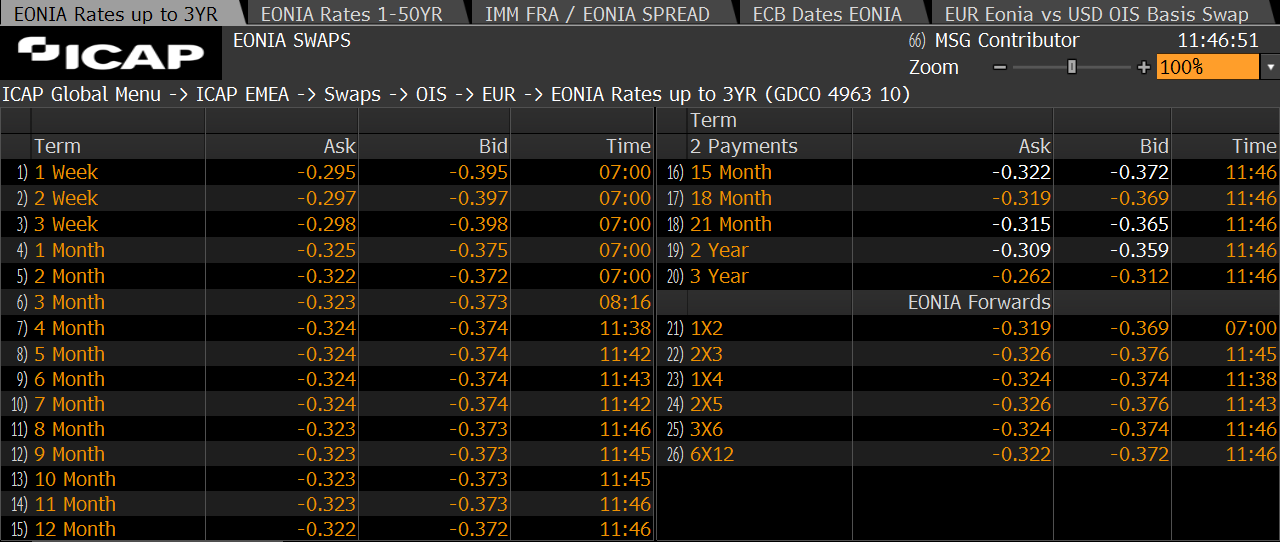
\includegraphics[width=1.\linewidth]{figures/icap_3.png}
\caption{Screenshot of market quotes from ICAP.}
\label{fig:icap}
\end{figure}

Though there exist some electronic platform in which market participants post bids and offers and other participants can apply them, in practice a lot of trading is still done over "voice", i.e.~by phone or more
commonly over chat. For convenience, however, Bloomberg provides a service which displays indicative real time rates as provided by a selection of relevant brokers. (\emph{N.B.~interest rate swap quotes vary from standard price quotes of commonly traded instruments, they can appear puzzling because the quotes are effectively interest rates})

In the following we use a similarly created data-set (\href{https://drive.google.com/file/d/1LCEDmheKqwPXFpJ25hFz32QI5im2UJO1/view?usp=sharing}{\texttt{ois\_data.xlsx}}) to derive our discount curve; with the help of the \texttt{pandas} module the data-set can be inspected:

\begin{tcolorbox}[breakable, size=fbox, boxrule=1pt, pad at break*=1mm,colback=cellbackground, colframe=cellborder]
\begin{Verbatim}[commandchars=\\\{\}]
\PY{k+kn}{import} \PY{n+nn}{pandas}\PY{o}{,} \PY{n+nn}{datetime}

\PY{n}{observation\PYZus{}date} \PY{o}{=} \PY{n}{datetime}\PY{o}{.}\PY{n}{date}\PY{o}{.}\PY{n}{today}\PY{p}{(}\PY{p}{)}

\PY{n}{mq} \PY{o}{=} \PY{n}{pandas}\PY{o}{.}\PY{n}{read\PYZus{}excel}\PY{p}{(}\PY{l+s+s1}{\PYZsq{}}\PY{l+s+s1}{ois\PYZus{}data.xlsx}\PY{l+s+s1}{\PYZsq{}}\PY{p}{)}
\PY{n}{mq}\PY{o}{.}\PY{n}{head}\PY{p}{(}\PY{p}{)}

   months  quote
0       1 -0.350
1       2 -0.347
2       3 -0.348
3       4 -0.350
4       5 -0.350
\end{Verbatim}
\end{tcolorbox}

Next we could convert the data-set into a dictionary for later usage or
use the \(\tt{DataFrame}\) directly, it is just matter of taste.

Let's say we want to build a 15 months swap instance using data
contained in \(\tt{ois\_data}\) file. Be careful when doing this
operation and double check the units of rates, quotes, etc\ldots{}in
this case for example quotes are expressed in percent so you need to
multiply them by 0.01 before using them. Another detail to check is that
15 months quote is not the fifteenth entry in the \(\tt{DataFrame}\)
(actually it is the twelfth).

\begin{tcolorbox}[breakable, size=fbox, boxrule=1pt, pad at break*=1mm, colback=cellbackground, colframe=cellborder]
\begin{Verbatim}[commandchars=\\\{\}]
\PY{n}{ois} \PY{o}{=} \PY{n}{OvernightIndexSwap}\PY{p}{(}\PY{l+m+mf}{1e6}\PY{p}{,}
                         \PY{p}{[}\PY{n}{date}\PY{p}{(}\PY{l+m+mi}{2019}\PY{p}{,} \PY{l+m+mi}{10}\PY{p}{,} \PY{l+m+mi}{23}\PY{p}{)}\PY{p}{,}
                          \PY{n}{date}\PY{p}{(}\PY{l+m+mi}{2020}\PY{p}{,} \PY{l+m+mi}{10}\PY{p}{,} \PY{l+m+mi}{23}\PY{p}{)}\PY{p}{,}
                          \PY{n}{date}\PY{p}{(}\PY{l+m+mi}{2020}\PY{p}{,} \PY{l+m+mi}{1}\PY{p}{,} \PY{l+m+mi}{23}\PY{p}{)}\PY{p}{]}\PY{p}{,}
                         \PY{n}{mq}\PY{p}{[}\PY{l+s+s1}{\PYZsq{}}\PY{l+s+s1}{quote}\PY{l+s+s1}{\PYZsq{}}\PY{p}{]}\PY{o}{.}\PY{n}{tolist}\PY{p}{(}\PY{p}{)}\PY{p}{[}\PY{l+m+mi}{12}\PY{p}{]}\PY{o}{*}\PY{l+m+mf}{0.01}\PY{p}{)}

\PY{c+c1}{\PYZsh{} print the last payment date }
\PY{c+c1}{\PYZsh{} (15 months after obs date)}
\PY{n}{ois}\PY{o}{.}\PY{n}{payment\PYZus{}dates}\PY{p}{[}\PY{o}{\PYZhy{}}\PY{l+m+mi}{1}\PY{p}{]}

datetime.date(2020, 1, 23)
\end{Verbatim}
\end{tcolorbox}

Clearly to use the \texttt{npv} method to calculate the OIS' NPV we need a discount curve with which to evaluate it and here comes to hand the bootstrapping technique !

\subsection{Constructing the Yield Curve}\label{the-bootstrapping-technique}

Keep aside for a moment our swaps and introduce the \emph{bootstrap
algorithm}. In finance, bootstrap is a method for constructing a
(zero-coupon) fixed-income yield curve from the prices of a set of
coupon-bearing products, e.g.~bonds and swaps. The term structure of
spot returns is obtained from the bond yields by solving for them
recursively, by forward substitution: this iterative process is what is
called the bootstrap method. The usefulness of bootstrap is that using
only a few carefully selected zero-coupon products, it becomes possible
to derive swap forward and spot rates for all maturities given the
solved curve.

To illustrate bootstrapping let's consider the following example which can be partially solved analytically: we have some coupon paying bond (coupon of 4\%, 5\%, 6\%, 7\% and 8\% respectively) with maturities ranging from 1 to 5 years, each having a value of \euro{100} and traded at par. To determine the zero-coupon yield curve proceed as follows:

\begin{enumerate}
\item at the end of the first year the $1^{st}$ bond will pay a coupon of \euro{4} (= \euro{100} * 4\%) plus the principal amount (= \euro{100}) which sums up to \euro{104} while the bond is trading at \euro{100}. Therefore, the implied 1-year spot \emph{fair} rate $S_{1y}$ can be calculated as, $\mbox{\euro{100}} = \mbox{\euro{104}} / (1 + S_{1y})$;

\item at the end of second year the sum of the cash flows of the $2^{nd}$ bond can be compared to its trading price to compute the 2-year spot rate $S_{2y}$ as $\mbox{\euro{100}} = \mbox{\euro{5}} / (1 + S_{1y}) + \mbox{\euro{105}} / (1 + S_{2y})^{2}$, using the previously derived value of $S_{1y}$;

\item at the end of third year the sum of the cash flows of the $3^{rd}$ bond can be compared to its trading price to calculate the 3-year spot rate $S_{3y}$ as $\mbox{\euro{100}} = \mbox{\euro{6}} / (1 + S_{1y}) + \mbox{\euro{6}} / (1 + S_{2y})^{2} + \mbox{\euro{106}} / (1 + S_{3y})^{3}$, using $S_{1y}$ and $S_{2y}$ computed before;

\item repeat the same reasoning for the other bonds.
\end{enumerate}

Putting all together we can construct a system of equations (now omitting the currency symbol for simplicity):

\begin{equation}
\begin{cases}
100 = \cfrac{104}{(1 + S_{1y})} \\
100 = \cfrac{5}{(1 + S_{1y})} + \cfrac{105}{(1 + S_{2y})^{2}} \\
100 = \cfrac{6} {(1 + S_{1y})} + \cfrac{6}{(1 + S_{2y})^{2}} + \cfrac{106} {(1 + S_{3y})^{3}} \\
100 = \cfrac{7} {(1 + S_{1y})} + \cfrac{7} {(1 + S_{2y})^{2}} + \cfrac{7} {(1 + S_{3y})^{3}} + \cfrac{107} {(1 + S_{4y})^{4}} \\
100 = \cfrac{8} {(1 + S_{1y})} + \cfrac{8} {(1 + S_{2y})^{2}}+ \cfrac{8} {(1 + S_{3y})^{3}} + \cfrac{8} {(1 + S_{4y})^{4}} + \cfrac{108} {(1 + S_{5y})^{5}}
\end{cases}
\label{eq:fifth_year_rate}
\end{equation}

This system can be solved quite easily: from the first equation can be derived $S_{1y}$, from the second $S_{2y}$, from the third $S_{3y}$ and so on. So

\[100 = 104 / (1 + S_{1y})\quad\Rightarrow\quad S_{1y} = 104/100 - 1 = 4\% \]

Moving to the second equation:

\begin{equation*}
\begin{split}
& 100 = 5 / (1 + 0.04) + 105 / (1 + S_{2y})^{2}\quad\Rightarrow\quad S_{2y}^2  + 2 S_{2y}  - 0.103030 = 0 \\
& S_{2y} = - 1 \pm \sqrt{1 + 0.103030} = \begin{cases}\text{\sout{-2.05023}} \\ 0.0503\end{cases}
\end{split}
\end{equation*}
where the first solution has been discarded because negative.

From the third one on it is not as simple to solve them analytically since involve third order (or more) equations, anyway it is possible to solve them numerically.
Assume we have found all the rates up to the fourth year (they are reported in Table~\ref{tab:rates}) and let's try to determine the last one.

\begin{table}[htb]
\begin{center}
\begin{tabular}{|c|c|c|c|}
\hline
\textbf{years} & \textbf{coupon rate} & \textbf{bond price} & \textbf{spot rate} \\
\hline
1 & 1.00 \% & \euro{100} & 4.00\% \\
\hline
2 & 2.00 \% & \euro{100} & 5.03\% \\
\hline
3 & 3.00 \% & \euro{100} & 6.08\% \\
\hline
4 & 4.00 \% & \euro{100} & 7.19\% \\
\hline
5 & 5.00 \% & \euro{100} & ??? \\
\hline
\end{tabular}
\end{center}
\caption{Table reporting maturity, coupon, bond price and implied spot rate for the example outlined in the text.}
\label{tab:rates}
\end{table}
The last column of Table~\ref{tab:rates} provides with the terms to fill the zero-coupon yield curve.
To solve the last equation numerically we can use the \texttt{scipy.optimize.brentq} function which finds the zeros of a user-defined function given a validity interval.
In Figure~\ref{fig:fifth_year_rate} the function to determine the 5 year rate expressed in the last of Eqs.~\ref{eq:fifth_year_rate} is shown. From the plot we expect tha rate to be around 8\%.

\begin{figure}[htb]
  \centering
  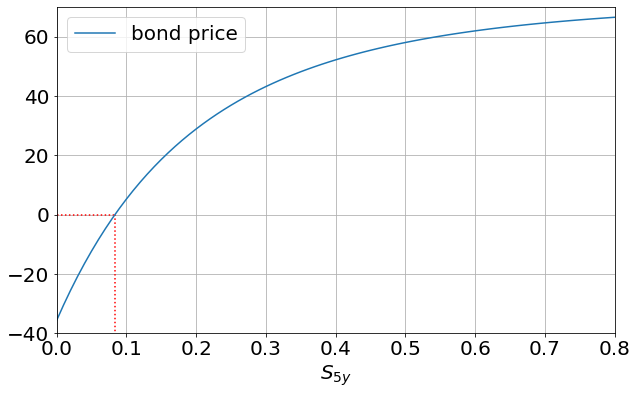
\includegraphics[width=0.7\textwidth]{figures/bond_5_plot.png}
  \caption{Plot of the discounted cash flow of bond 5 as a function of the 5 year spot rate.}
  \label{fig:fifth_year_rate}
\end{figure}

\begin{tcolorbox}[breakable, size=fbox, boxrule=1pt, pad at break*=1mm,colback=cellbackground, colframe=cellborder]
\begin{Verbatim}[commandchars=\\\{\}]
\PY{k+kn}{from} \PY{n+nn}{scipy}\PY{n+nn}{.}\PY{n+nn}{optimize} \PY{k}{import} \PY{n}{brentq}

\PY{k}{def} \PY{n+nf}{func}\PY{p}{(}\PY{n}{x}\PY{p}{)}\PY{p}{:}
    \PY{k}{return} \PY{l+m+mi}{100} \PY{o}{\PYZhy{}} \PY{l+m+mi}{8}\PY{o}{/}\PY{p}{(}\PY{l+m+mi}{1}\PY{o}{+}\PY{l+m+mf}{0.04}\PY{p}{)} \PY{o}{\PYZhy{}} \PY{l+m+mi}{8}\PY{o}{/}\PY{p}{(}\PY{l+m+mi}{1}\PY{o}{+}\PY{l+m+mf}{0.0503}\PY{p}{)}\PY{o}{*}\PY{o}{*}\PY{l+m+mi}{2} \PY{o}{\PYZhy{}} \PY{l+m+mi}{8}\PY{o}{/}\PY{p}{(}\PY{l+m+mi}{1}\PY{o}{+}\PY{l+m+mf}{0.0608}\PY{p}{)}\PY{o}{*}\PY{o}{*}\PY{l+m+mi}{3} 
               \PY{o}{\PYZhy{}} \PY{l+m+mi}{8}\PY{o}{/}\PY{p}{(}\PY{l+m+mi}{1}\PY{o}{+}\PY{l+m+mf}{0.0719}\PY{p}{)}\PY{o}{*}\PY{o}{*}\PY{l+m+mi}{4} \PY{o}{\PYZhy{}} \PY{l+m+mi}{108}\PY{o}{/}\PY{p}{(}\PY{l+m+mi}{1}\PY{o}{+}\PY{n}{x}\PY{p}{)}\PY{o}{*}\PY{o}{*}\PY{l+m+mi}{5}

\PY{n}{a} \PY{o}{=} \PY{n}{brentq}\PY{p}{(}\PY{n}{func}\PY{p}{,} \PY{l+m+mi}{0}\PY{p}{,} \PY{l+m+mf}{0.10}\PY{p}{)}
\PY{n+nb}{print} \PY{p}{(}\PY{l+s+s2}{\PYZdq{}}\PY{l+s+s2}{5y rate: }\PY{l+s+si}{\PYZob{}:.4f\PYZcb{}}\PY{l+s+s2}{\PYZdq{}}\PY{o}{.}\PY{n}{format}\PY{p}{(}\PY{n}{a}\PY{p}{)}\PY{p}{)}

5y rate: 0.0836
\end{Verbatim}
\end{tcolorbox}

The very same mechanism can be generalized and extended to more maturities to get a more detailed yield curve. In general terms the previous system can be written as:

\begin{equation*}
\begin{cases}
f_1(S_1, p_1) = 0 \\
f_2(S_1, S_2, p_2) = 0 \\
f_3(S_1, S_2, S_3, p_3) = 0 \\
f_4(S_1, S_2, S_3, S_4, p_4) = 0 \\
\cdots
\end{cases}
\end{equation*}
where $S_i$ are the unknown spot rates and $p_i$ the prices of the considered products. The iterative procedure we have applied before exploits the first equation to find $S_1 = f_1^{-1}(p_1)$, the second to find $S_2 = f_2^{-1}(S_1, p_2)$ and so on and so forth; this algorithm works since each equation will determine exactly one \emph{free} spot rate which is not already determined by the others.

\subsection{Bootstrap as Minimization Problem}
We can now describe the bootstrapping algorithm in general terms as follows:
\begin{enumerate}
\item define a set of yielding products , these will generally be coupon-bearing bonds;
\item derive discount factors for the corresponding terms;
\item \emph{bootstrap} the zero-coupon curve, successively calibrating the curve such that it returns the prices of these inputs.
\end{enumerate}

Instead of iteratively finding the solution of each equation as before, we could define a vector of spot rates $\mathbf{S} = (S_1, S_2, S_3, \ldots)$ seeking for a particular $\mathbf{\hat{S}}$ which solves the following equation:

\begin{equation*}
F = f_1^2(\hat{S}_1) + f_2^2(\hat{S}_1, \hat{S}_2) + f_3^2(\hat{S}_1, \hat{S}_2, \hat{S}_3) + f_4^2(\hat{S}_1, \hat{S}_2, \hat{S}_3, \hat{S}_4) + \ldots = 0
\end{equation*}

Under this terms bootstrapping can be considered as a minimization algorithm, indeed we need to find $\mathbf{\hat{S}}$ which \emph{minimize} $F$, or makes it as close as possible to 0.
Notice how each \(f_i\) is squared since we want all of them to be minimized and
not only \(F\) globally (without the squared there may be cancellation
effects between the terms of the sum).

\subsection{Minimization Algorithm}\label{minimization-algorithm}

A minimization algorithm follows these steps:

\begin{itemize}
\tightlist
\item
  define an \emph{objective function} i.e.~the function that is actually
  minimized to reach our goal;
\item
  set the initial value of the unknown parameters and their range of
  variability;
\item
  the minimizer will compute the objective function value;
\item
  then it will move the parameter values in such a way to find a smaller
  value of the objective function (e.g.~following the derivative w.r.t.
  each parameter);
\item if constraints are defined, they will be considered in the previous step;
\item
  the last three steps will be repeated until further variations of the
  \(\mathbf{x}\) values won't change significantly the objective
  function (i.e.~we have found a minimum of the function so the
  minimization process is completed !).
\end{itemize}

Let's see with a couple of example how minimization can be implemented in \texttt{python} using the function \texttt{scipy.optimize.minimize}.

\subsubsection{Example}\label{example}

Find the dimensions that will minimize the cost to
manufacture a circular cylindrical can of volume, \(330~\mathrm{cm}^3\), see Figure~\ref{fig:cylinder}.

\begin{figure}[h]
\centering
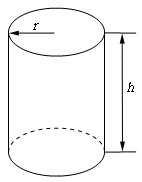
\includegraphics[width=0.2\textwidth]{figures/cylinder.png}
\caption{Graphical representation of the \emph{can} minimization example.}
\label{fig:cylinder}
\end{figure}

Clearly to minimize the costs the company needs to reduce the can
surface, given the required volume.

\[ S = 2\pi rh + 2\cdot(\pi r^2) \]

On the other hand we want the volume to be \(330~\mathrm{cm}^3\) so we
can remove \(h\) from the previous equation:

\[ V = \pi r^2 h = 330\quad\implies h = \cfrac{330}{\pi r^2} \]

So in the end the surface function to be minimized is:

\[ S = 2\pi rh + 2\cdot(\pi r^2) = \cfrac{2\cdot 330}{r} + 2\cdot(\pi r^2)\]

So we implement the objective function, \(\tt{x[0]}\) is the can radius:

\begin{tcolorbox}[breakable, size=fbox, boxrule=1pt, pad at break*=1mm,colback=cellbackground, colframe=cellborder]
\begin{Verbatim}[commandchars=\\\{\}]
\PY{k+kn}{from} \PY{n+nn}{math} \PY{k}{import} \PY{n}{pi}

\PY{k}{def} \PY{n+nf}{of}\PY{p}{(}\PY{n}{x}\PY{p}{)}\PY{p}{:}
    \PY{k}{return} \PY{l+m+mi}{2}\PY{o}{*}\PY{l+m+mi}{330}\PY{o}{/}\PY{n}{x}\PY{p}{[}\PY{l+m+mi}{0}\PY{p}{]} \PY{o}{+} \PY{l+m+mi}{2}\PY{o}{*}\PY{n}{pi}\PY{o}{*}\PY{n}{x}\PY{p}{[}\PY{l+m+mi}{0}\PY{p}{]}\PY{o}{*}\PY{o}{*}\PY{l+m+mi}{2}
\end{Verbatim}
\end{tcolorbox}

Set the limits to our unknown variable and its initial value:

\begin{tcolorbox}[breakable, size=fbox, boxrule=1pt, pad at break*=1mm,colback=cellbackground, colframe=cellborder]
\begin{Verbatim}[commandchars=\\\{\}]
\PY{n}{x0} \PY{o}{=} \PY{p}{[}\PY{l+m+mi}{1}\PY{p}{]}
\PY{n}{bounds} \PY{o}{=} \PY{p}{[}\PY{p}{(}\PY{l+m+mf}{0.01}\PY{p}{,} \PY{l+m+mi}{100}\PY{p}{)}\PY{p}{]}
\end{Verbatim}
\end{tcolorbox}

    Finally we run the minimization:

    \begin{tcolorbox}[breakable, size=fbox, boxrule=1pt, pad at break*=1mm,colback=cellbackground, colframe=cellborder]
\begin{Verbatim}[commandchars=\\\{\}]
\PY{n}{r} \PY{o}{=} \PY{n}{minimize}\PY{p}{(}\PY{n}{of}\PY{p}{,} \PY{n}{x0}\PY{p}{,} \PY{n}{bounds}\PY{o}{=}\PY{n}{bounds}\PY{p}{)}
\PY{n+nb}{print} \PY{p}{(}\PY{n}{r}\PY{p}{)}

      fun: 264.356810914805
 hess\_inv: <1x1 LbfgsInvHessProduct with dtype=float64>
      jac: array([5.68434189e-06])
  message: b'CONVERGENCE: NORM\_OF\_PROJECTED\_GRADIENT\_<=\_PGTOL'
     nfev: 24
      nit: 9
   status: 0
  success: True
        x: array([3.7449385])
    \end{Verbatim}
\end{tcolorbox}

    So to minimize the cost the company should produce cans with a radius of
about 3.745 cm (I suspect that Coke have done a similar calculation...).

\subsubsection{Example with Constraint}\label{example-with-constraint}

We are going to fence in a rectangular field. If we look at the field
from above the cost of the vertical sides are \$10/m, the cost of the
bottom is \$2/m and the cost of the top is \$7/m. If we have \$700 determine
the dimensions of the field that will maximize the enclosed area, see Fig.~\ref{fig:field}.

\begin{figure}[h]
\centering
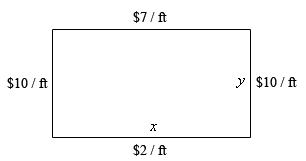
\includegraphics[width=0.4\textwidth]{figures/field.png}
\caption{Graphical representation of the \emph{field} minimization example.}
\label{fig:field}
\end{figure}

In this example there are two differences with respect to the previous one:

\begin{itemize}
\tightlist
\item
  we want to maximize a quantity (not minimize);
\item
  there is a constraint (we have a limited amount of money).
\end{itemize}

So let's repeat the steps as before. The objective is to maximize the
enclosed area \(A\) but we are able to just minimize so we can define in the objective function the quantity \(-A\), if we minimize it
we will maximize the area $A$. Define the length and the width of the field with \(\tt{x[0]}\) and
\(\tt{x[1]}\) (items of the list \(\tt{x}\):

    \begin{tcolorbox}[breakable, size=fbox, boxrule=1pt, pad at break*=1mm,colback=cellbackground, colframe=cellborder]
\begin{Verbatim}[commandchars=\\\{\}]
\PY{k}{def} \PY{n+nf}{of}\PY{p}{(}\PY{n}{x}\PY{p}{)}\PY{p}{:}
    \PY{k}{return} \PY{o}{\PYZhy{}} \PY{n}{x}\PY{p}{[}\PY{l+m+mi}{0}\PY{p}{]}\PY{o}{*}\PY{n}{x}\PY{p}{[}\PY{l+m+mi}{1}\PY{p}{]}
\end{Verbatim}
\end{tcolorbox}

    Now we can set the boundaries for length and width and their initial
values (1 m each):

    \begin{tcolorbox}[breakable, size=fbox, boxrule=1pt, pad at break*=1mm,colback=cellbackground, colframe=cellborder]
\begin{Verbatim}[commandchars=\\\{\}]
\PY{n}{x0} \PY{o}{=} \PY{p}{[}\PY{l+m+mi}{1}\PY{p}{,} \PY{l+m+mi}{1}\PY{p}{]}
\PY{n}{bounds} \PY{o}{=} \PY{p}{[}\PY{p}{(}\PY{l+m+mf}{0.01}\PY{p}{,} \PY{l+m+mi}{100}\PY{p}{)} \PY{k}{for} \PY{n}{\PYZus{}} \PY{o+ow}{in} \PY{n+nb}{range}\PY{p}{(}\PY{n+nb}{len}\PY{p}{(}\PY{n}{x0}\PY{p}{)}\PY{p}{)}\PY{p}{]}
\end{Verbatim}
\end{tcolorbox}

    We have also to impose the constraint on the money. This is done by
defining a function that compute the money spent with the fence and
compare it to \$700. The constraint is passed to the minimizer with a
dictionary which has two keys: \(\tt{type}\) with value \(\tt{eq}\)
(like equality) since we want to spend all of our available money so the
fence has to cost \$700

\[\mathrm{fence~cost} = l\cdot10 + l\cdot10 + w\cdot2 + w\cdot7 = 700\]
\[700 - l\cdot10 - l\cdot10 - w\cdot2 - w\cdot7 = 0\],
\(\tt{fun}\) whose value is the constraint function.

\begin{tcolorbox}[breakable, size=fbox, boxrule=1pt, pad at break*=1mm,colback=cellbackground, colframe=cellborder]
\begin{Verbatim}[commandchars=\\\{\}]
\PY{k}{def} \PY{n+nf}{cons}\PY{p}{(}\PY{n}{x}\PY{p}{)}\PY{p}{:}
    \PY{k}{return} \PY{l+m+mi}{700} \PY{o}{\PYZhy{}} \PY{n}{x}\PY{p}{[}\PY{l+m+mi}{0}\PY{p}{]}\PY{o}{*}\PY{l+m+mi}{20} \PY{o}{\PYZhy{}} \PY{n}{x}\PY{p}{[}\PY{l+m+mi}{1}\PY{p}{]}\PY{o}{*}\PY{l+m+mi}{2} \PY{o}{\PYZhy{}} \PY{n}{x}\PY{p}{[}\PY{l+m+mi}{1}\PY{p}{]}\PY{o}{*}\PY{l+m+mi}{7}

\PY{n}{constraints} \PY{o}{=} \PY{p}{\PYZob{}}\PY{l+s+s1}{\PYZsq{}}\PY{l+s+s1}{type}\PY{l+s+s1}{\PYZsq{}}\PY{p}{:}\PY{l+s+s1}{\PYZsq{}}\PY{l+s+s1}{eq}\PY{l+s+s1}{\PYZsq{}}\PY{p}{,} \PY{l+s+s1}{\PYZsq{}}\PY{l+s+s1}{fun}\PY{l+s+s1}{\PYZsq{}}\PY{p}{:}\PY{n}{cons}\PY{p}{\PYZcb{}}
\end{Verbatim}
\end{tcolorbox}

    Now we can call the minimizer.

    \begin{tcolorbox}[breakable, size=fbox, boxrule=1pt, pad at break*=1mm,colback=cellbackground, colframe=cellborder]
\begin{Verbatim}[commandchars=\\\{\}]
\PY{n}{r} \PY{o}{=} \PY{n}{minimize}\PY{p}{(}\PY{n}{of}\PY{p}{,} \PY{n}{x0}\PY{p}{,} \PY{n}{bounds}\PY{o}{=}\PY{n}{bounds}\PY{p}{,} \PY{n}{constraints}\PY{o}{=}\PY{n}{constraints}\PY{p}{)}
\PY{n+nb}{print} \PY{p}{(}\PY{n}{r}\PY{p}{)}

     fun: -680.5555555555482
     jac: array([-38.88889313, -17.5       ])
 message: 'Optimization terminated successfully.'
    nfev: 16
     nit: 4
    njev: 4
  status: 0
 success: True
       x: array([17.49999818, 38.88889293])
    \end{Verbatim}
\end{tcolorbox}

So the field will come out \(17.5\)m long and \(38.9\)m wide.

\subsection{Local Minima}
When the objective function has local minima the choice of the initial value of the parameters can be critical. 
Assume we would like to minimize an objective function like 

\[
f(x) = \cfrac{\mathrm{cos}(3\pi x)}{x}
\]
This function is plotted in Fig.~\ref{fig:local_minima} in the range $[0, 2]$, and it is clear that it has many minima. 

\begin{figure}[htb]
	\centering
	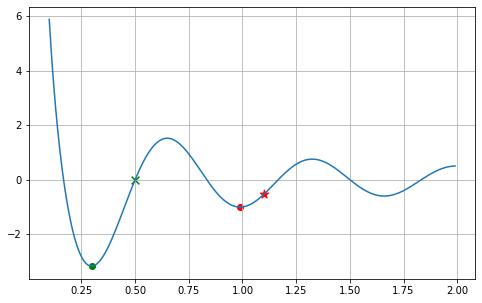
\includegraphics[width=0.7\textwidth]{figures/lesson4_39_0.png}
\caption{Plot of an example function with many local minima. The red points highlights initial value and minimum found in a \emph{bad} minimization, green points for a good minimization.}
\label{fig:local_minima}
\end{figure}

Let's try to find a minimum and set the initial value to $x=1.1$.
\begin{tcolorbox}[breakable, size=fbox, boxrule=1pt, pad at break*=1mm,colback=cellbackground, colframe=cellborder]
\begin{Verbatim}[commandchars=\\\{\}]
\PY{k+kn}{from} \PY{n+nn}{scipy}\PY{n+nn}{.}\PY{n+nn}{optimize} \PY{k}{import} \PY{n}{minimize}
\PY{n}{x0} \PY{o}{=} \PY{p}{[}\PY{l+m+mf}{1.1}\PY{p}{]}
\PY{n}{bounds} \PY{o}{=} \PY{p}{[}\PY{p}{(}\PY{l+m+mf}{0.01}\PY{p}{,} \PY{l+m+mi}{20}\PY{p}{)}\PY{p}{]}
		
\PY{n}{r} \PY{o}{=} \PY{n}{minimize}\PY{p}{(}\PY{n}{func}\PY{p}{,} \PY{n}{x0}\PY{p}{,} \PY{n}{bounds}\PY{o}{=}\PY{n}{bounds}\PY{p}{)}
\PY{n}{r}

fun: array([-1.00569871])
hess\_inv: <1x1 LbfgsInvHessProduct with dtype=float64>
jac: array([-4.4408921e-07])
message: b'CONVERGENCE: NORM\_OF\_PROJECTED\_GRADIENT\_<=\_PGTOL'
nfev: 16
nit: 5
status: 0
success: True
x: array([0.98865633])
\end{Verbatim}
\end{tcolorbox}
The minimization worked perfectly and we found $x=0.98865633$ (i.e. the red point in Fig.~\ref{fig:local_minima}) but still from the same Figure it is clear that this is not the absolute minimum we would like to find. The problem arise since the algorithm has got stuck in this local minimum without any possibility to jump out from the well.

If we repeat the minimization using as initial value $0.5$ instead
\begin{tcolorbox}[breakable, size=fbox, boxrule=1pt, pad at break*=1mm,colback=cellbackground, colframe=cellborder]
\begin{Verbatim}[commandchars=\\\{\}]
\PY{k+kn}{from} \PY{n+nn}{scipy}\PY{n+nn}{.}\PY{n+nn}{optimize} \PY{k}{import} \PY{n}{minimize}
\PY{n}{x0} \PY{o}{=} \PY{p}{[}\PY{l+m+mf}{0.5}\PY{p}{]}
\PY{n}{bounds} \PY{o}{=} \PY{p}{[}\PY{p}{(}\PY{l+m+mf}{0.01}\PY{p}{,} \PY{l+m+mi}{20}\PY{p}{)}\PY{p}{]}
		
\PY{n}{r} \PY{o}{=} \PY{n}{minimize}\PY{p}{(}\PY{n}{func}\PY{p}{,} \PY{n}{x0}\PY{p}{,} \PY{n}{bounds}\PY{o}{=}\PY{n}{bounds}\PY{p}{)}
\PY{n}{r}

fun: array([-3.17151711])
hess\_inv: <1x1 LbfgsInvHessProduct with dtype=float64>
jac: array([9.76996262e-07])
message: b'CONVERGENCE: NORM\_OF\_PROJECTED\_GRADIENT\_<=\_PGTOL'
nfev: 16
nit: 5
status: 0
success: True
x: array([0.29691798])
\end{Verbatim}
\end{tcolorbox}
Now clearly the algorithm found the absolute minimum in $x=0.29691798$ (i.e. the green point in Fig.~\ref{fig:local_minima}) because there was no chance to find a local minimum during the iterations.

This is clearly an example of what could happen, the possible solution is to make a \emph{scan} of the objective function to try to approximately determine where the global minimum is and choose the \emph{right} initial values for our parameters.
There should be such an issue in the application of the bootstrapping algorithm though since the function that we are going to minimize is a sum of squared terms which has no local minima, just a global minimum (i.e. it is a parabola).


\subsection{OIS Example}\label{ois-example}
Back to our Overnight Index Swap, the general idea here is to get the discount curve \(\mathcal{C}\) such that it prices correctly each OIS by minimizing the sum of their NPV squared (our \(f_i\)):

\[\mathrm{min}_{\mathcal{C}} \Big\{\sum_{i=1}^{n}\mathrm{NPV}(\mathrm{OIS}_i, \mathcal{C})^2\Big\}\]

A discount curve is characterized by pillar dates and the corresponding discount factors. The description of the problem we have given above does not, in theory, specifies any constraint on the number of pillar dates of the discount curve \(\mathcal{C}\). However, the pillar dates determine the number of unknown variables (i.e.~the dimensionality \(N\) of the optimization problem). A curve with \(N\) pillar dates has \(N\) discount factors (note that the first discount factor with value date equal to the today date, is constrained to 1). \textbf{In practice, therefore, it makes sense to choose the pillar dates in such a way that there are exactly the right number of degrees of freedom in the optimization to match data.} So the natural choice is to choose the pillar dates of the discount curve equal to the set of expiry dates of the swaps.

Once we've fixed \(\mathbf{d}\) to be a vector of pillar dates equal to the expiry dates of the swaps, and we use the notation \(\mathbf{x}\) to represent the vector of pillar discount factors, then the problem becomes:

\[\mathrm{min}_{\mathbf{x}} \Big\{\sum_{i=1}^{N}\mathrm{NPV}(\mathrm{OIS}_i, \mathcal{C}(\mathbf{d}, \mathbf{x}))^2\Big\}\]
which is our optimization problem (\textbf{to find the minimum of the
above expression as a function of x}) that can be solved using one of
the available numerical optimization routines in \(\tt{python}\).

So first let's create the swaps according to all the available market
quotes and also the pillar dates of our final discount curve:

    \begin{tcolorbox}[breakable, size=fbox, boxrule=1pt, pad at break*=1mm,colback=cellbackground, colframe=cellborder]
\begin{Verbatim}[commandchars=\\\{\}]
\PY{k+kn}{from} \PY{n+nn}{finmarkets} \PY{k}{import} \PY{n}{generate\PYZus{}swap\PYZus{}dates}

\PY{n}{observation\PYZus{}date} \PY{o}{=} \PY{n}{date}\PY{p}{(}\PY{l+m+mi}{2019}\PY{p}{,} \PY{l+m+mi}{10}\PY{p}{,} \PY{l+m+mi}{23}\PY{p}{)}
\PY{n}{pillar\PYZus{}dates} \PY{o}{=} \PY{p}{[}\PY{n}{observation\PYZus{}date}\PY{p}{]}
\PY{n}{swaps} \PY{o}{=} \PY{p}{[}\PY{p}{]} \PY{c+c1}{\PYZsh{} container of the OIS objects}

\PY{k}{for} \PY{n}{i} \PY{o+ow}{in} \PY{n+nb}{range}\PY{p}{(}\PY{n+nb}{len}\PY{p}{(}\PY{n}{df}\PY{p}{)}\PY{p}{)}\PY{p}{:}
    \PY{n}{swap} \PY{o}{=} \PY{n}{OvernightIndexSwap}\PY{p}{(}\PY{l+m+mf}{1e6}\PY{p}{,}
                    \PY{n}{generate\PYZus{}swap\PYZus{}dates}\PY{p}{(}
                        \PY{n}{observation\PYZus{}date}\PY{p}{,} 
                        \PY{n}{mq}\PY{p}{[}\PY{l+s+s1}{\PYZsq{}}\PY{l+s+s1}{months}\PY{l+s+s1}{\PYZsq{}}\PY{p}{]}\PY{o}{.}\PY{n}{tolist}\PY{p}{(}\PY{p}{)}\PY{p}{[}\PY{n}{i}\PY{p}{]}\PY{p}{)}\PY{p}{,}
                    \PY{l+m+mf}{0.01} \PY{o}{*} \PY{n}{mq}\PY{p}{[}\PY{l+s+s1}{\PYZsq{}}\PY{l+s+s1}{quote}\PY{l+s+s1}{\PYZsq{}}\PY{p}{]}\PY{o}{.}\PY{n}{tolist}\PY{p}{(}\PY{p}{)}\PY{p}{[}\PY{n}{i}\PY{p}{]}\PY{p}{)}

    \PY{n}{swaps}\PY{o}{.}\PY{n}{append}\PY{p}{(}\PY{n}{swap}\PY{p}{)}
    \PY{n}{pillar\PYZus{}dates}\PY{o}{.}\PY{n}{append}\PY{p}{(}\PY{n}{swap}\PY{o}{.}\PY{n}{payment\PYZus{}dates}\PY{p}{[}\PY{o}{\PYZhy{}}\PY{l+m+mi}{1}\PY{p}{]}\PY{p}{)}

\PY{c+c1}{\PYZsh{} this shouldn\PYZsq{}t be necessary if the original}
\PY{c+c1}{\PYZsh{} list of market quotes is sorted}
\PY{n}{pillar\PYZus{}dates} \PY{o}{=} \PY{n+nb}{sorted}\PY{p}{(}\PY{n}{pillar\PYZus{}dates}\PY{p}{)}
\end{Verbatim}
\end{tcolorbox}

So let's implement the method with the swaps we have just created, of course we don't need to write our minimisation algorithm since we can use the one provided by \texttt{python} which is defined in \texttt{scipy.optimize}, function \texttt{minimize}.

\begin{itemize}
\tightlist
\item
  define the objective function: the sum of the squared NPVs of the OIS

    \begin{tcolorbox}[breakable, size=fbox, boxrule=1pt, pad at break*=1mm,colback=cellbackground, colframe=cellborder]
\begin{Verbatim}[commandchars=\\\{\}]
\PY{k}{def} \PY{n+nf}{objective\PYZus{}function}\PY{p}{(}\PY{n}{x}\PY{p}{)}\PY{p}{:}
    \PY{n}{curve} \PY{o}{=} \PY{n}{DiscountCurve}\PY{p}{(}\PY{n}{observation\PYZus{}date}\PY{p}{,}
                          \PY{n}{pillar\PYZus{}dates}\PY{p}{,}
                          \PY{n}{x}\PY{p}{)}
    
    \PY{n}{sum\PYZus{}sq} \PY{o}{=} \PY{l+m+mf}{0.0}
    \PY{k}{for} \PY{n}{swap} \PY{o+ow}{in} \PY{n}{swaps}\PY{p}{:}
        \PY{n}{sum\PYZus{}sq} \PY{o}{+}\PY{o}{=} \PY{n}{swap}\PY{o}{.}\PY{n}{npv}\PY{p}{(}\PY{n}{curve}\PY{p}{)} \PY{o}{*}\PY{o}{*} \PY{l+m+mi}{2}
    \PY{k}{return} \PY{n}{sum\PYZus{}sq}
\end{Verbatim}
\end{tcolorbox}

\item
  set the initial value of the discount factors (\(x_i^0\)) to 1 with a
  range of variability \([ 0.01, 10]\), in addition the first element of
  the list, today's discount factor, will be fixed to 1 (variability
  \([1, 1]\))

    \begin{tcolorbox}[breakable, size=fbox, boxrule=1pt, pad at break*=1mm,colback=cellbackground, colframe=cellborder]
\begin{Verbatim}[commandchars=\\\{\}]
\PY{n}{x0} \PY{o}{=} \PY{p}{[}\PY{l+m+mf}{1.0} \PY{k}{for} \PY{n}{i} \PY{o+ow}{in} \PY{n+nb}{range}\PY{p}{(}\PY{n+nb}{len}\PY{p}{(}\PY{n}{pillar\PYZus{}dates}\PY{p}{)}\PY{p}{)}\PY{p}{]}

\PY{n}{bounds} \PY{o}{=} \PY{p}{[}\PY{p}{(}\PY{l+m+mf}{0.01}\PY{p}{,} \PY{l+m+mf}{10.0}\PY{p}{)} \PY{k}{for} \PY{n}{i} \PY{o+ow}{in} \PY{n+nb}{range}\PY{p}{(}\PY{n+nb}{len}\PY{p}{(}\PY{n}{pillar\PYZus{}dates}\PY{p}{)}\PY{p}{)}\PY{p}{]}
\PY{n}{bounds}\PY{p}{[}\PY{l+m+mi}{0}\PY{p}{]} \PY{o}{=} \PY{p}{(}\PY{l+m+mf}{1.0}\PY{p}{,} \PY{l+m+mf}{1.0}\PY{p}{)}
\end{Verbatim}
\end{tcolorbox}

\item
  finally we can launch the minimizer to find the discount factors
  (\(x\))

    \begin{tcolorbox}[breakable, size=fbox, boxrule=1pt, pad at break*=1mm,colback=cellbackground, colframe=cellborder]
\begin{Verbatim}[commandchars=\\\{\}]
\PY{k+kn}{from} \PY{n+nn}{scipy}\PY{n+nn}{.}\PY{n+nn}{optimize} \PY{k}{import} \PY{n}{minimize}

\PY{n}{result} \PY{o}{=} \PY{n}{minimize}\PY{p}{(}\PY{n}{objective\PYZus{}function}\PY{p}{,} \PY{n}{x0}\PY{p}{,} \PY{n}{bounds}\PY{o}{=}\PY{n}{bounds}\PY{p}{)}
\PY{n+nb}{print} \PY{p}{(}\PY{n}{result}\PY{p}{)}
\end{Verbatim}
\end{tcolorbox}

    \begin{Verbatim}[commandchars=\\\{\}]
      fun: 0.000819919032900304
 hess\_inv: <34x34 LbfgsInvHessProduct with dtype=float64>
      jac: array([ 6.58948735e+05, -1.58720803e+01, -6.53143264e+01,
-1.03323232e+02,
       -1.26050260e+02, -1.31748898e+02, -1.20374599e+02, -9.15399651e+01,
       -4.24363322e+01,  2.44903182e+01,  1.14345243e+02,  2.22002243e+02,
       -3.72021700e+00,  4.21398633e+01,  4.21787852e+01,  4.22369487e+01,
        4.23327026e+01,  4.31814758e+01,  4.44924460e+01,  4.62078978e+01,
        4.82906823e+01, -3.69972738e+00, -1.42454702e+00,  7.53771932e-01,
        2.79741018e+00,  4.62896699e+00,  6.24844054e+00,  9.93101553e+00,
        1.31122434e+01,  1.42880909e+01,  1.48279215e+01,  1.50787019e+01,
        1.43267935e+01,  1.38451324e+01])
  message: b'CONVERGENCE: REL\_REDUCTION\_OF\_F\_<=\_FACTR*EPSMCH'
     nfev: 840
      nit: 7
   status: 0
  success: True
        x: array([1.        , 1.00030147, 1.00058831, 1.00089012, 1.00119726,
       1.00147996, 1.00178743, 1.00208107, 1.00238467, 1.00267865,
       1.00298261, 1.00327737, 1.00357104, 1.00357104, 1.00355063,
       1.00352002, 1.00346901, 1.00302007, 1.00232627, 1.00141821,
       1.00031629, 0.99911234, 0.99790839, 0.99675545, 0.99567393,
       0.99470465, 0.9938476 , 0.99189884, 0.99021534, 0.98959296,
       0.98930728, 0.98917464, 0.98957256, 0.98982763])
    \end{Verbatim}
\end{itemize}

Printing the result gives us the a lot of information about the minimisation just performed, the most useful are:
\begin{itemize}
\item \texttt{func}: the value of the objective function at the last iteration;
\item \texttt{message}: the summary message from the algorithm (if it is \texttt{CONVERGENCE} is OK);
\item \texttt{success}: the name is self explanatory;
\item \texttt{x}: the vector of unknown parameters that have been optimised.
\end{itemize}

Another useful check to perform in order to understand if everything went fine, is the comparison of the objective function with the initial guessed parameters and at the end of the minimisation.

\begin{tcolorbox}[breakable, size=fbox, boxrule=1pt, pad at break*=1mm,colback=cellbackground, colframe=cellborder]
\begin{Verbatim}[commandchars=\\\{\}]
\PY{n+nb}{print} \PY{p}{(}\PY{l+s+s2}{\PYZdq{}}\PY{l+s+s2}{Initial objective function value }\PY{l+s+s2}{\PYZdq{}}\PY{p}{,} \PY{n}{objective\PYZus{}function}\PY{p}{(}\PY{n}{x0}\PY{p}{)}\PY{p}{)}
\PY{n+nb}{print} \PY{p}{(}\PY{l+s+s2}{\PYZdq{}}\PY{l+s+s2}{Final objective function value }\PY{l+s+s2}{\PYZdq{}}\PY{p}{,} \PY{n}{objective\PYZus{}function}\PY{p}{(}\PY{n}{result}\PY{o}{.}\PY{n}{x}\PY{p}{)}\PY{p}{)}

Initial objective function value  931188216.6666666
Final objective function value  0.000819919032900304
    \end{Verbatim}
\end{tcolorbox}
The objective function at the end of the minimisation is not exactly 0 (and rarely it will be) but its value is small enough for us to be satisfied, we started with $10^{10}$ and now it is $10^{-4}$ so 14 orders of magnitude smaller. This means that with the derived discount curve the NPV's of our OIS won't be identically 0 but so small that we can consider them as they were.

It can be very useful to also look at some diagnostic plots to check if the minimization was successful. Figure~\ref{fig:minimization_diagnostic} reports on the left the objective function value as a function of discount factor $(x_1)$; clearly we have found a minimum (the orange point represent $x_1$ value at the end of the minimization). On the right the value of the objective function at each iteration is shown instead, its value is decreasing dramatically (notice that the $y$ axis is drawn in log scale).

\begin{figure}[htb]
  \centering
  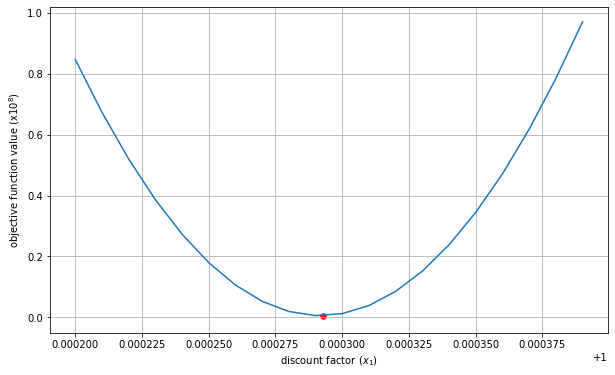
\includegraphics[width=0.45\linewidth]{figures/obj_func.png}
  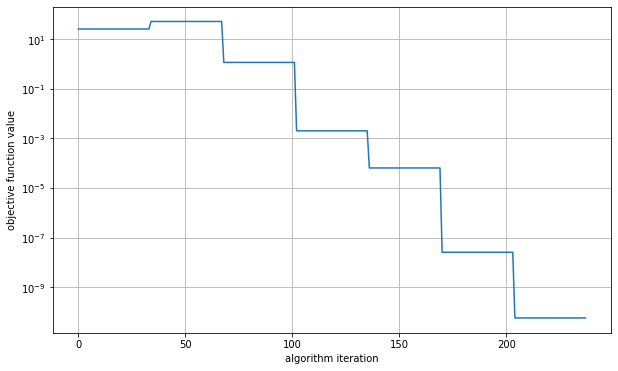
\includegraphics[width=0.45\linewidth]{figures/obj_func_iter.png}
  \caption{Diagnostic plots for the minimization algorithm. On the left the objective function value as a function of the discount factor $x_1$, on the right the objective function value as a function of the iteration number (the orange point represent $x_1$ value at the end of the minimization).}
  \label{fig:minimization_diagnostic}
\end{figure}

Finally we can create the discount curve implied by the market quote of
our swaps (see Fig.~\ref{fig:discount_curve}) and try to compute some implied rate.

\begin{tcolorbox}[breakable, size=fbox, boxrule=1pt, pad at break*=1mm,colback=cellbackground, colframe=cellborder]
\begin{Verbatim}[commandchars=\\\{\}]
\PY{k+kn}{from} \PY{n+nn}{math} \PY{k}{import} \PY{n}{log}
\PY{n}{curve} \PY{o}{=} \PY{n}{DiscountCurve}\PY{p}{(}\PY{n}{observation\PYZus{}date}\PY{p}{,} \PY{n}{pillar\PYZus{}dates}\PY{p}{,} \PY{n}{result}\PY{o}{.}\PY{n}{x}\PY{p}{)}

\PY{n}{d} \PY{o}{=} \PY{n}{date}\PY{p}{(}\PY{l+m+mi}{2059}\PY{p}{,} \PY{l+m+mi}{11}\PY{p}{,} \PY{l+m+mi}{23}\PY{p}{)}
\PY{n+nb}{print} \PY{p}{(}\PY{l+s+s2}{\PYZdq{}}\PY{l+s+s2}{40y df: }\PY{l+s+si}{\PYZob{}\PYZcb{}}\PY{l+s+s2}{\PYZdq{}}\PY{o}{.}\PY{n}{format}\PY{p}{(}\PY{n}{curve}\PY{o}{.}\PY{n}{df}\PY{p}{(}\PY{n}{d}\PY{p}{)}\PY{p}{)}\PY{p}{)}
\PY{n+nb}{print} \PY{p}{(}\PY{l+s+s2}{\PYZdq{}}\PY{l+s+s2}{40y rate: }\PY{l+s+si}{\PYZob{}\PYZcb{}}\PY{l+s+s2}{\PYZdq{}}\PY{o}{.}\PY{n}{format}\PY{p}{(}\PY{o}{\PYZhy{}}\PY{n}{log}\PY{p}{(}\PY{n}{curve}\PY{o}{.}\PY{n}{df}\PY{p}{(}\PY{n}{d}\PY{p}{)}\PY{p}{)} \PY{o}{/} \PY{l+m+mi}{40}\PY{p}{)}\PY{p}{)}             

40y df: 0.9891780176191146
40y rate: 0.0002720241491103593
    \end{Verbatim}
\end{tcolorbox}

\begin{figure}[htb]
  \centering
  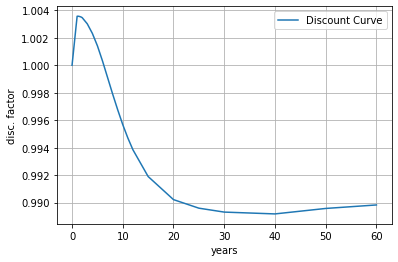
\includegraphics[width=0.7\textwidth]{figures/bootstrap_23_0.png}
  \caption{Plot of the discount curve implied by Overnight Index Swap market quotes.}
  \label{fig:discount_curve}
\end{figure}


\clearpage
\documentclass[11pt]{article}

    \usepackage[breakable]{tcolorbox}
    \usepackage{parskip} % Stop auto-indenting (to mimic markdown behaviour)
    
    \usepackage{iftex}
    \ifPDFTeX
    	\usepackage[T1]{fontenc}
    	\usepackage{mathpazo}
    \else
    	\usepackage{fontspec}
    \fi

    % Basic figure setup, for now with no caption control since it's done
    % automatically by Pandoc (which extracts ![](path) syntax from Markdown).
    \usepackage{graphicx}
    % Ensure that by default, figures have no caption (until we provide a
    % proper Figure object with a Caption API and a way to capture that
    % in the conversion process - todo).
    %\usepackage{caption}
    %\DeclareCaptionFormat{nocaption}{}
    %\captionsetup{format=nocaption,aboveskip=0pt,belowskip=0pt}

    \usepackage[Export]{adjustbox} % Used to constrain images to a maximum size
    \adjustboxset{max size={0.9\linewidth}{0.9\paperheight}}
    \usepackage{float}
    \floatplacement{figure}{H} % forces figures to be placed at the correct location
    \usepackage{xcolor} % Allow colors to be defined
    \usepackage{enumerate} % Needed for markdown enumerations to work
    \usepackage{geometry} % Used to adjust the document margins
    \usepackage{amsmath} % Equations
    \usepackage{amssymb} % Equations
    \usepackage{textcomp} % defines textquotesingle
    % Hack from http://tex.stackexchange.com/a/47451/13684:
    \AtBeginDocument{%
        \def\PYZsq{\textquotesingle}% Upright quotes in Pygmentized code
    }
    \usepackage{upquote} % Upright quotes for verbatim code
    \usepackage{eurosym} % defines \euro
    \usepackage[mathletters]{ucs} % Extended unicode (utf-8) support
    \usepackage{fancyvrb} % verbatim replacement that allows latex
    \usepackage{grffile} % extends the file name processing of package graphics 
                         % to support a larger range
    \makeatletter % fix for grffile with XeLaTeX
    \def\Gread@@xetex#1{%
      \IfFileExists{"\Gin@base".bb}%
      {\Gread@eps{\Gin@base.bb}}%
      {\Gread@@xetex@aux#1}%
    }
    \makeatother

    % The hyperref package gives us a pdf with properly built
    % internal navigation ('pdf bookmarks' for the table of contents,
    % internal cross-reference links, web links for URLs, etc.)
    \usepackage{hyperref}
    % The default LaTeX title has an obnoxious amount of whitespace. By default,
    % titling removes some of it. It also provides customization options.
    \usepackage{titling}
    \usepackage{longtable} % longtable support required by pandoc >1.10
    \usepackage{booktabs}  % table support for pandoc > 1.12.2
    \usepackage[inline]{enumitem} % IRkernel/repr support (it uses the enumerate* environment)
    \usepackage[normalem]{ulem} % ulem is needed to support strikethroughs (\sout)
                                % normalem makes italics be italics, not underlines
    \usepackage{mathrsfs}
    

    
    % Colors for the hyperref package
    \definecolor{urlcolor}{rgb}{0,.145,.698}
    \definecolor{linkcolor}{rgb}{.71,0.21,0.01}
    \definecolor{citecolor}{rgb}{.12,.54,.11}

    % ANSI colors
    \definecolor{ansi-black}{HTML}{3E424D}
    \definecolor{ansi-black-intense}{HTML}{282C36}
    \definecolor{ansi-red}{HTML}{E75C58}
    \definecolor{ansi-red-intense}{HTML}{B22B31}
    \definecolor{ansi-green}{HTML}{00A250}
    \definecolor{ansi-green-intense}{HTML}{007427}
    \definecolor{ansi-yellow}{HTML}{DDB62B}
    \definecolor{ansi-yellow-intense}{HTML}{B27D12}
    \definecolor{ansi-blue}{HTML}{208FFB}
    \definecolor{ansi-blue-intense}{HTML}{0065CA}
    \definecolor{ansi-magenta}{HTML}{D160C4}
    \definecolor{ansi-magenta-intense}{HTML}{A03196}
    \definecolor{ansi-cyan}{HTML}{60C6C8}
    \definecolor{ansi-cyan-intense}{HTML}{258F8F}
    \definecolor{ansi-white}{HTML}{C5C1B4}
    \definecolor{ansi-white-intense}{HTML}{A1A6B2}
    \definecolor{ansi-default-inverse-fg}{HTML}{FFFFFF}
    \definecolor{ansi-default-inverse-bg}{HTML}{000000}

    % commands and environments needed by pandoc snippets
    % extracted from the output of `pandoc -s`
    \providecommand{\tightlist}{%
      \setlength{\itemsep}{0pt}\setlength{\parskip}{0pt}}
    \DefineVerbatimEnvironment{Highlighting}{Verbatim}{commandchars=\\\{\}}
    % Add ',fontsize=\small' for more characters per line
    \newenvironment{Shaded}{}{}
    \newcommand{\KeywordTok}[1]{\textcolor[rgb]{0.00,0.44,0.13}{\textbf{{#1}}}}
    \newcommand{\DataTypeTok}[1]{\textcolor[rgb]{0.56,0.13,0.00}{{#1}}}
    \newcommand{\DecValTok}[1]{\textcolor[rgb]{0.25,0.63,0.44}{{#1}}}
    \newcommand{\BaseNTok}[1]{\textcolor[rgb]{0.25,0.63,0.44}{{#1}}}
    \newcommand{\FloatTok}[1]{\textcolor[rgb]{0.25,0.63,0.44}{{#1}}}
    \newcommand{\CharTok}[1]{\textcolor[rgb]{0.25,0.44,0.63}{{#1}}}
    \newcommand{\StringTok}[1]{\textcolor[rgb]{0.25,0.44,0.63}{{#1}}}
    \newcommand{\CommentTok}[1]{\textcolor[rgb]{0.38,0.63,0.69}{\textit{{#1}}}}
    \newcommand{\OtherTok}[1]{\textcolor[rgb]{0.00,0.44,0.13}{{#1}}}
    \newcommand{\AlertTok}[1]{\textcolor[rgb]{1.00,0.00,0.00}{\textbf{{#1}}}}
    \newcommand{\FunctionTok}[1]{\textcolor[rgb]{0.02,0.16,0.49}{{#1}}}
    \newcommand{\RegionMarkerTok}[1]{{#1}}
    \newcommand{\ErrorTok}[1]{\textcolor[rgb]{1.00,0.00,0.00}{\textbf{{#1}}}}
    \newcommand{\NormalTok}[1]{{#1}}
    
    % Additional commands for more recent versions of Pandoc
    \newcommand{\ConstantTok}[1]{\textcolor[rgb]{0.53,0.00,0.00}{{#1}}}
    \newcommand{\SpecialCharTok}[1]{\textcolor[rgb]{0.25,0.44,0.63}{{#1}}}
    \newcommand{\VerbatimStringTok}[1]{\textcolor[rgb]{0.25,0.44,0.63}{{#1}}}
    \newcommand{\SpecialStringTok}[1]{\textcolor[rgb]{0.73,0.40,0.53}{{#1}}}
    \newcommand{\ImportTok}[1]{{#1}}
    \newcommand{\DocumentationTok}[1]{\textcolor[rgb]{0.73,0.13,0.13}{\textit{{#1}}}}
    \newcommand{\AnnotationTok}[1]{\textcolor[rgb]{0.38,0.63,0.69}{\textbf{\textit{{#1}}}}}
    \newcommand{\CommentVarTok}[1]{\textcolor[rgb]{0.38,0.63,0.69}{\textbf{\textit{{#1}}}}}
    \newcommand{\VariableTok}[1]{\textcolor[rgb]{0.10,0.09,0.49}{{#1}}}
    \newcommand{\ControlFlowTok}[1]{\textcolor[rgb]{0.00,0.44,0.13}{\textbf{{#1}}}}
    \newcommand{\OperatorTok}[1]{\textcolor[rgb]{0.40,0.40,0.40}{{#1}}}
    \newcommand{\BuiltInTok}[1]{{#1}}
    \newcommand{\ExtensionTok}[1]{{#1}}
    \newcommand{\PreprocessorTok}[1]{\textcolor[rgb]{0.74,0.48,0.00}{{#1}}}
    \newcommand{\AttributeTok}[1]{\textcolor[rgb]{0.49,0.56,0.16}{{#1}}}
    \newcommand{\InformationTok}[1]{\textcolor[rgb]{0.38,0.63,0.69}{\textbf{\textit{{#1}}}}}
    \newcommand{\WarningTok}[1]{\textcolor[rgb]{0.38,0.63,0.69}{\textbf{\textit{{#1}}}}}
    
    
    % Define a nice break command that doesn't care if a line doesn't already
    % exist.
    \def\br{\hspace*{\fill} \\* }
    % Math Jax compatibility definitions
    \def\gt{>}
    \def\lt{<}
    \let\Oldtex\TeX
    \let\Oldlatex\LaTeX
    \renewcommand{\TeX}{\textrm{\Oldtex}}
    \renewcommand{\LaTeX}{\textrm{\Oldlatex}}
    % Document parameters
    % Document title
    \title{Machine Lerning}
    \author{Matteo Sani\\\href{mailto:matteosan1@gmail.com}{matteosan1@gmail.com}}
    
    
    
    
    
% Pygments definitions
\makeatletter
\def\PY@reset{\let\PY@it=\relax \let\PY@bf=\relax%
    \let\PY@ul=\relax \let\PY@tc=\relax%
    \let\PY@bc=\relax \let\PY@ff=\relax}
\def\PY@tok#1{\csname PY@tok@#1\endcsname}
\def\PY@toks#1+{\ifx\relax#1\empty\else%
    \PY@tok{#1}\expandafter\PY@toks\fi}
\def\PY@do#1{\PY@bc{\PY@tc{\PY@ul{%
    \PY@it{\PY@bf{\PY@ff{#1}}}}}}}
\def\PY#1#2{\PY@reset\PY@toks#1+\relax+\PY@do{#2}}

\expandafter\def\csname PY@tok@w\endcsname{\def\PY@tc##1{\textcolor[rgb]{0.73,0.73,0.73}{##1}}}
\expandafter\def\csname PY@tok@c\endcsname{\let\PY@it=\textit\def\PY@tc##1{\textcolor[rgb]{0.25,0.50,0.50}{##1}}}
\expandafter\def\csname PY@tok@cp\endcsname{\def\PY@tc##1{\textcolor[rgb]{0.74,0.48,0.00}{##1}}}
\expandafter\def\csname PY@tok@k\endcsname{\let\PY@bf=\textbf\def\PY@tc##1{\textcolor[rgb]{0.00,0.50,0.00}{##1}}}
\expandafter\def\csname PY@tok@kp\endcsname{\def\PY@tc##1{\textcolor[rgb]{0.00,0.50,0.00}{##1}}}
\expandafter\def\csname PY@tok@kt\endcsname{\def\PY@tc##1{\textcolor[rgb]{0.69,0.00,0.25}{##1}}}
\expandafter\def\csname PY@tok@o\endcsname{\def\PY@tc##1{\textcolor[rgb]{0.40,0.40,0.40}{##1}}}
\expandafter\def\csname PY@tok@ow\endcsname{\let\PY@bf=\textbf\def\PY@tc##1{\textcolor[rgb]{0.67,0.13,1.00}{##1}}}
\expandafter\def\csname PY@tok@nb\endcsname{\def\PY@tc##1{\textcolor[rgb]{0.00,0.50,0.00}{##1}}}
\expandafter\def\csname PY@tok@nf\endcsname{\def\PY@tc##1{\textcolor[rgb]{0.00,0.00,1.00}{##1}}}
\expandafter\def\csname PY@tok@nc\endcsname{\let\PY@bf=\textbf\def\PY@tc##1{\textcolor[rgb]{0.00,0.00,1.00}{##1}}}
\expandafter\def\csname PY@tok@nn\endcsname{\let\PY@bf=\textbf\def\PY@tc##1{\textcolor[rgb]{0.00,0.00,1.00}{##1}}}
\expandafter\def\csname PY@tok@ne\endcsname{\let\PY@bf=\textbf\def\PY@tc##1{\textcolor[rgb]{0.82,0.25,0.23}{##1}}}
\expandafter\def\csname PY@tok@nv\endcsname{\def\PY@tc##1{\textcolor[rgb]{0.10,0.09,0.49}{##1}}}
\expandafter\def\csname PY@tok@no\endcsname{\def\PY@tc##1{\textcolor[rgb]{0.53,0.00,0.00}{##1}}}
\expandafter\def\csname PY@tok@nl\endcsname{\def\PY@tc##1{\textcolor[rgb]{0.63,0.63,0.00}{##1}}}
\expandafter\def\csname PY@tok@ni\endcsname{\let\PY@bf=\textbf\def\PY@tc##1{\textcolor[rgb]{0.60,0.60,0.60}{##1}}}
\expandafter\def\csname PY@tok@na\endcsname{\def\PY@tc##1{\textcolor[rgb]{0.49,0.56,0.16}{##1}}}
\expandafter\def\csname PY@tok@nt\endcsname{\let\PY@bf=\textbf\def\PY@tc##1{\textcolor[rgb]{0.00,0.50,0.00}{##1}}}
\expandafter\def\csname PY@tok@nd\endcsname{\def\PY@tc##1{\textcolor[rgb]{0.67,0.13,1.00}{##1}}}
\expandafter\def\csname PY@tok@s\endcsname{\def\PY@tc##1{\textcolor[rgb]{0.73,0.13,0.13}{##1}}}
\expandafter\def\csname PY@tok@sd\endcsname{\let\PY@it=\textit\def\PY@tc##1{\textcolor[rgb]{0.73,0.13,0.13}{##1}}}
\expandafter\def\csname PY@tok@si\endcsname{\let\PY@bf=\textbf\def\PY@tc##1{\textcolor[rgb]{0.73,0.40,0.53}{##1}}}
\expandafter\def\csname PY@tok@se\endcsname{\let\PY@bf=\textbf\def\PY@tc##1{\textcolor[rgb]{0.73,0.40,0.13}{##1}}}
\expandafter\def\csname PY@tok@sr\endcsname{\def\PY@tc##1{\textcolor[rgb]{0.73,0.40,0.53}{##1}}}
\expandafter\def\csname PY@tok@ss\endcsname{\def\PY@tc##1{\textcolor[rgb]{0.10,0.09,0.49}{##1}}}
\expandafter\def\csname PY@tok@sx\endcsname{\def\PY@tc##1{\textcolor[rgb]{0.00,0.50,0.00}{##1}}}
\expandafter\def\csname PY@tok@m\endcsname{\def\PY@tc##1{\textcolor[rgb]{0.40,0.40,0.40}{##1}}}
\expandafter\def\csname PY@tok@gh\endcsname{\let\PY@bf=\textbf\def\PY@tc##1{\textcolor[rgb]{0.00,0.00,0.50}{##1}}}
\expandafter\def\csname PY@tok@gu\endcsname{\let\PY@bf=\textbf\def\PY@tc##1{\textcolor[rgb]{0.50,0.00,0.50}{##1}}}
\expandafter\def\csname PY@tok@gd\endcsname{\def\PY@tc##1{\textcolor[rgb]{0.63,0.00,0.00}{##1}}}
\expandafter\def\csname PY@tok@gi\endcsname{\def\PY@tc##1{\textcolor[rgb]{0.00,0.63,0.00}{##1}}}
\expandafter\def\csname PY@tok@gr\endcsname{\def\PY@tc##1{\textcolor[rgb]{1.00,0.00,0.00}{##1}}}
\expandafter\def\csname PY@tok@ge\endcsname{\let\PY@it=\textit}
\expandafter\def\csname PY@tok@gs\endcsname{\let\PY@bf=\textbf}
\expandafter\def\csname PY@tok@gp\endcsname{\let\PY@bf=\textbf\def\PY@tc##1{\textcolor[rgb]{0.00,0.00,0.50}{##1}}}
\expandafter\def\csname PY@tok@go\endcsname{\def\PY@tc##1{\textcolor[rgb]{0.53,0.53,0.53}{##1}}}
\expandafter\def\csname PY@tok@gt\endcsname{\def\PY@tc##1{\textcolor[rgb]{0.00,0.27,0.87}{##1}}}
\expandafter\def\csname PY@tok@err\endcsname{\def\PY@bc##1{\setlength{\fboxsep}{0pt}\fcolorbox[rgb]{1.00,0.00,0.00}{1,1,1}{\strut ##1}}}
\expandafter\def\csname PY@tok@kc\endcsname{\let\PY@bf=\textbf\def\PY@tc##1{\textcolor[rgb]{0.00,0.50,0.00}{##1}}}
\expandafter\def\csname PY@tok@kd\endcsname{\let\PY@bf=\textbf\def\PY@tc##1{\textcolor[rgb]{0.00,0.50,0.00}{##1}}}
\expandafter\def\csname PY@tok@kn\endcsname{\let\PY@bf=\textbf\def\PY@tc##1{\textcolor[rgb]{0.00,0.50,0.00}{##1}}}
\expandafter\def\csname PY@tok@kr\endcsname{\let\PY@bf=\textbf\def\PY@tc##1{\textcolor[rgb]{0.00,0.50,0.00}{##1}}}
\expandafter\def\csname PY@tok@bp\endcsname{\def\PY@tc##1{\textcolor[rgb]{0.00,0.50,0.00}{##1}}}
\expandafter\def\csname PY@tok@fm\endcsname{\def\PY@tc##1{\textcolor[rgb]{0.00,0.00,1.00}{##1}}}
\expandafter\def\csname PY@tok@vc\endcsname{\def\PY@tc##1{\textcolor[rgb]{0.10,0.09,0.49}{##1}}}
\expandafter\def\csname PY@tok@vg\endcsname{\def\PY@tc##1{\textcolor[rgb]{0.10,0.09,0.49}{##1}}}
\expandafter\def\csname PY@tok@vi\endcsname{\def\PY@tc##1{\textcolor[rgb]{0.10,0.09,0.49}{##1}}}
\expandafter\def\csname PY@tok@vm\endcsname{\def\PY@tc##1{\textcolor[rgb]{0.10,0.09,0.49}{##1}}}
\expandafter\def\csname PY@tok@sa\endcsname{\def\PY@tc##1{\textcolor[rgb]{0.73,0.13,0.13}{##1}}}
\expandafter\def\csname PY@tok@sb\endcsname{\def\PY@tc##1{\textcolor[rgb]{0.73,0.13,0.13}{##1}}}
\expandafter\def\csname PY@tok@sc\endcsname{\def\PY@tc##1{\textcolor[rgb]{0.73,0.13,0.13}{##1}}}
\expandafter\def\csname PY@tok@dl\endcsname{\def\PY@tc##1{\textcolor[rgb]{0.73,0.13,0.13}{##1}}}
\expandafter\def\csname PY@tok@s2\endcsname{\def\PY@tc##1{\textcolor[rgb]{0.73,0.13,0.13}{##1}}}
\expandafter\def\csname PY@tok@sh\endcsname{\def\PY@tc##1{\textcolor[rgb]{0.73,0.13,0.13}{##1}}}
\expandafter\def\csname PY@tok@s1\endcsname{\def\PY@tc##1{\textcolor[rgb]{0.73,0.13,0.13}{##1}}}
\expandafter\def\csname PY@tok@mb\endcsname{\def\PY@tc##1{\textcolor[rgb]{0.40,0.40,0.40}{##1}}}
\expandafter\def\csname PY@tok@mf\endcsname{\def\PY@tc##1{\textcolor[rgb]{0.40,0.40,0.40}{##1}}}
\expandafter\def\csname PY@tok@mh\endcsname{\def\PY@tc##1{\textcolor[rgb]{0.40,0.40,0.40}{##1}}}
\expandafter\def\csname PY@tok@mi\endcsname{\def\PY@tc##1{\textcolor[rgb]{0.40,0.40,0.40}{##1}}}
\expandafter\def\csname PY@tok@il\endcsname{\def\PY@tc##1{\textcolor[rgb]{0.40,0.40,0.40}{##1}}}
\expandafter\def\csname PY@tok@mo\endcsname{\def\PY@tc##1{\textcolor[rgb]{0.40,0.40,0.40}{##1}}}
\expandafter\def\csname PY@tok@ch\endcsname{\let\PY@it=\textit\def\PY@tc##1{\textcolor[rgb]{0.25,0.50,0.50}{##1}}}
\expandafter\def\csname PY@tok@cm\endcsname{\let\PY@it=\textit\def\PY@tc##1{\textcolor[rgb]{0.25,0.50,0.50}{##1}}}
\expandafter\def\csname PY@tok@cpf\endcsname{\let\PY@it=\textit\def\PY@tc##1{\textcolor[rgb]{0.25,0.50,0.50}{##1}}}
\expandafter\def\csname PY@tok@c1\endcsname{\let\PY@it=\textit\def\PY@tc##1{\textcolor[rgb]{0.25,0.50,0.50}{##1}}}
\expandafter\def\csname PY@tok@cs\endcsname{\let\PY@it=\textit\def\PY@tc##1{\textcolor[rgb]{0.25,0.50,0.50}{##1}}}

\def\PYZbs{\char`\\}
\def\PYZus{\char`\_}
\def\PYZob{\char`\{}
\def\PYZcb{\char`\}}
\def\PYZca{\char`\^}
\def\PYZam{\char`\&}
\def\PYZlt{\char`\<}
\def\PYZgt{\char`\>}
\def\PYZsh{\char`\#}
\def\PYZpc{\char`\%}
\def\PYZdl{\char`\$}
\def\PYZhy{\char`\-}
\def\PYZsq{\char`\'}
\def\PYZdq{\char`\"}
\def\PYZti{\char`\~}
% for compatibility with earlier versions
\def\PYZat{@}
\def\PYZlb{[}
\def\PYZrb{]}
\makeatother


    % For linebreaks inside Verbatim environment from package fancyvrb. 
    \makeatletter
        \newbox\Wrappedcontinuationbox 
        \newbox\Wrappedvisiblespacebox 
        \newcommand*\Wrappedvisiblespace {\textcolor{red}{\textvisiblespace}} 
        \newcommand*\Wrappedcontinuationsymbol {\textcolor{red}{\llap{\tiny$\m@th\hookrightarrow$}}} 
        \newcommand*\Wrappedcontinuationindent {3ex } 
        \newcommand*\Wrappedafterbreak {\kern\Wrappedcontinuationindent\copy\Wrappedcontinuationbox} 
        % Take advantage of the already applied Pygments mark-up to insert 
        % potential linebreaks for TeX processing. 
        %        {, <, #, %, $, ' and ": go to next line. 
        %        _, }, ^, &, >, - and ~: stay at end of broken line. 
        % Use of \textquotesingle for straight quote. 
        \newcommand*\Wrappedbreaksatspecials {% 
            \def\PYGZus{\discretionary{\char`\_}{\Wrappedafterbreak}{\char`\_}}% 
            \def\PYGZob{\discretionary{}{\Wrappedafterbreak\char`\{}{\char`\{}}% 
            \def\PYGZcb{\discretionary{\char`\}}{\Wrappedafterbreak}{\char`\}}}% 
            \def\PYGZca{\discretionary{\char`\^}{\Wrappedafterbreak}{\char`\^}}% 
            \def\PYGZam{\discretionary{\char`\&}{\Wrappedafterbreak}{\char`\&}}% 
            \def\PYGZlt{\discretionary{}{\Wrappedafterbreak\char`\<}{\char`\<}}% 
            \def\PYGZgt{\discretionary{\char`\>}{\Wrappedafterbreak}{\char`\>}}% 
            \def\PYGZsh{\discretionary{}{\Wrappedafterbreak\char`\#}{\char`\#}}% 
            \def\PYGZpc{\discretionary{}{\Wrappedafterbreak\char`\%}{\char`\%}}% 
            \def\PYGZdl{\discretionary{}{\Wrappedafterbreak\char`\$}{\char`\$}}% 
            \def\PYGZhy{\discretionary{\char`\-}{\Wrappedafterbreak}{\char`\-}}% 
            \def\PYGZsq{\discretionary{}{\Wrappedafterbreak\textquotesingle}{\textquotesingle}}% 
            \def\PYGZdq{\discretionary{}{\Wrappedafterbreak\char`\"}{\char`\"}}% 
            \def\PYGZti{\discretionary{\char`\~}{\Wrappedafterbreak}{\char`\~}}% 
        } 
        % Some characters . , ; ? ! / are not pygmentized. 
        % This macro makes them "active" and they will insert potential linebreaks 
        \newcommand*\Wrappedbreaksatpunct {% 
            \lccode`\~`\.\lowercase{\def~}{\discretionary{\hbox{\char`\.}}{\Wrappedafterbreak}{\hbox{\char`\.}}}% 
            \lccode`\~`\,\lowercase{\def~}{\discretionary{\hbox{\char`\,}}{\Wrappedafterbreak}{\hbox{\char`\,}}}% 
            \lccode`\~`\;\lowercase{\def~}{\discretionary{\hbox{\char`\;}}{\Wrappedafterbreak}{\hbox{\char`\;}}}% 
            \lccode`\~`\:\lowercase{\def~}{\discretionary{\hbox{\char`\:}}{\Wrappedafterbreak}{\hbox{\char`\:}}}% 
            \lccode`\~`\?\lowercase{\def~}{\discretionary{\hbox{\char`\?}}{\Wrappedafterbreak}{\hbox{\char`\?}}}% 
            \lccode`\~`\!\lowercase{\def~}{\discretionary{\hbox{\char`\!}}{\Wrappedafterbreak}{\hbox{\char`\!}}}% 
            \lccode`\~`\/\lowercase{\def~}{\discretionary{\hbox{\char`\/}}{\Wrappedafterbreak}{\hbox{\char`\/}}}% 
            \catcode`\.\active
            \catcode`\,\active 
            \catcode`\;\active
            \catcode`\:\active
            \catcode`\?\active
            \catcode`\!\active
            \catcode`\/\active 
            \lccode`\~`\~ 	
        }
    \makeatother

    \let\OriginalVerbatim=\Verbatim
    \makeatletter
    \renewcommand{\Verbatim}[1][1]{%
        %\parskip\z@skip
        \sbox\Wrappedcontinuationbox {\Wrappedcontinuationsymbol}%
        \sbox\Wrappedvisiblespacebox {\FV@SetupFont\Wrappedvisiblespace}%
        \def\FancyVerbFormatLine ##1{\hsize\linewidth
            \vtop{\raggedright\hyphenpenalty\z@\exhyphenpenalty\z@
                \doublehyphendemerits\z@\finalhyphendemerits\z@
                \strut ##1\strut}%
        }%
        % If the linebreak is at a space, the latter will be displayed as visible
        % space at end of first line, and a continuation symbol starts next line.
        % Stretch/shrink are however usually zero for typewriter font.
        \def\FV@Space {%
            \nobreak\hskip\z@ plus\fontdimen3\font minus\fontdimen4\font
            \discretionary{\copy\Wrappedvisiblespacebox}{\Wrappedafterbreak}
            {\kern\fontdimen2\font}%
        }%
        
        % Allow breaks at special characters using \PYG... macros.
        \Wrappedbreaksatspecials
        % Breaks at punctuation characters . , ; ? ! and / need catcode=\active 	
        \OriginalVerbatim[#1,codes*=\Wrappedbreaksatpunct]%
    }
    \makeatother

    % Exact colors from NB
    \definecolor{incolor}{HTML}{303F9F}
    \definecolor{outcolor}{HTML}{D84315}
    \definecolor{cellborder}{HTML}{CFCFCF}
    \definecolor{cellbackground}{HTML}{F7F7F7}
    
    % prompt
    \makeatletter
    \newcommand{\boxspacing}{\kern\kvtcb@left@rule\kern\kvtcb@boxsep}
    \makeatother
    \newcommand{\prompt}[4]{
        \ttfamily\llap{{\color{#2}[#3]:\hspace{3pt}#4}}\vspace{-\baselineskip}
    }
    

    
    % Prevent overflowing lines due to hard-to-break entities
    \sloppy 
    % Setup hyperref package
    \hypersetup{
      breaklinks=true,  % so long urls are correctly broken across lines
      colorlinks=true,
      urlcolor=urlcolor,
      linkcolor=linkcolor,
      citecolor=citecolor,
      }
    % Slightly bigger margins than the latex defaults
    
    \geometry{verbose,tmargin=1in,bmargin=1in,lmargin=1in,rmargin=1in}
    
    

\begin{document}
    
    \maketitle
    
    

    
    \hypertarget{neural-network---practical-lesson-8}{%
\section{Neural Network - Practical Lesson
8}\label{neural-network---practical-lesson-8}}

\hypertarget{overview}{%
\subsection{Overview}\label{overview}}

In this lesson we will see how machine learning techniques can be
successfully applied to solve financial problems. We will first do a
quick tour on the theory behind neural networks and then we will see an
example and two practical applications regarding regression and
classification issues.

\textbf{Disclaimer}: this lecture just scratches the surface of the
machine learning topic which has seen a huge development in the latest
years leading to thousands of applications in many different fields.

\hypertarget{neural-networks}{%
\subsection{Neural networks}\label{neural-networks}}

\hypertarget{definition}{%
\subsubsection{Definition}\label{definition}}

Artificial Neural Networks (ANN or simply NN) are information processing
models that are developed by inspiring from the working principles of
human brain. Their most essential property is the ability of learning
from sample sets.

The basic process units of ANN architecture are neurons which are
internally in connection with other neurons.

\begin{figure}
\centering
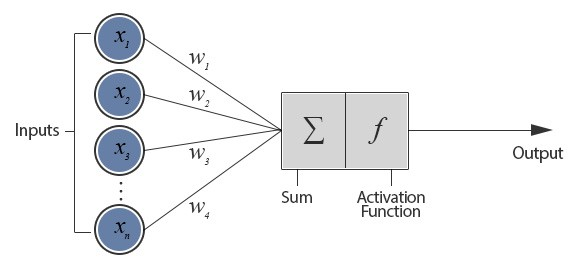
\includegraphics[width=0.8\linewidth]{neuron.jpeg}
\caption{Model of an artificial neuron.}
\end{figure}

A neuron consists of weights (\(w_i\)) and real (\(x_i\)) numbers. All
inputs injected into neurons are individually weighted, added together
and passed into the activation function which produce the neuron output.
There are many different types of activation function but one of the
simplest would be \emph{step function} which returns just 0 or 1
according to the input value (another is the \emph{sigmoid} which can be
thought of as the continuous version of the step function).

\begin{figure}
\centering
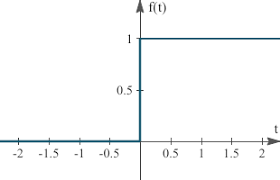
\includegraphics[width=0.4\linewidth]{step_function.png}
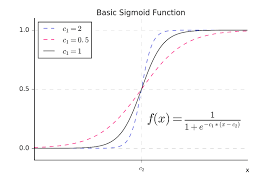
\includegraphics[width=0.4\linewidth]{sigmoid.png}
\caption{On the left an example of step function on the right a sigmoid.}
\end{figure}

\hypertarget{training-of-a-neuron}{%
\subsubsection{Training of a neuron}\label{training-of-a-neuron}}

When teaching children how to recognize a bus, we just tell them,
showing an example: ``This is a bus. That is not a bus.'' until they
learn the concept of what a bus is. Furthermore, if the child sees new
objects that she hasn't seen before, we could expect her to recognize
correctly whether the new object is a bus or not. This is exactly the
idea behind the neurons. Similarly, inputs from a \emph{training} set
are presented to the neuron one after the other and the neuron weights
are modified according to the expected output.

When an entire pass through all of the input training vectors is
completed the neuron has learnt ! At this time, if an input vector
\(\vec{P}\) (already in the training set) is given to the neuron, it
will output the correct value. If \(\vec{P}\) is not in the training
set, the network will respond with an output similar to other training
vectors close to \(\vec{P}\).

Unfortunately using just a neuron is not too useful since it is not
possible to solve the interesting problems we would like to face with
just that simple architecture. The next step is then to put together
more neurons in \emph{layers}.

\hypertarget{multi-layered-neural-networks}{%
\subsubsection{Multi-layered neural
networks}\label{multi-layered-neural-networks}}

\begin{figure}
\centering
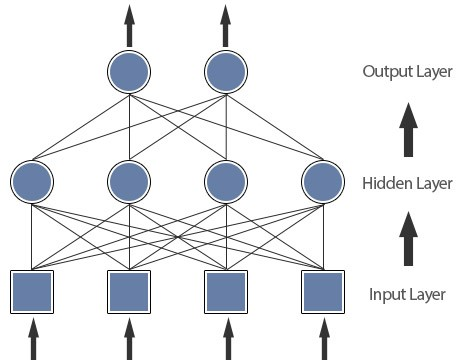
\includegraphics[width=0.7\linewidth]{multilayer.jpeg}
\caption{A multi-layered neural network.}
\end{figure}

Each input from the \emph{input layer} is fed up to each node in the
hidden layer, and from there to each node on the output layer. We should
note that there can be any number of nodes per layer and there are
usually multiple hidden layers to pass through before ultimately
reaching the output layer. But to train this network we need a learning
algorithm which should be able to tune not only the weights between the
output layer and the hidden layer but also the weights between the
hidden layer and the input layer.

\hypertarget{back-propagation}{%
\subsubsection{Back propagation}\label{back-propagation}}

In order to tune the weights at each layer at every iteration we should
know what the output would be at each node. But this is not possbile
since the only value we know is the correct output at the last node (the
final output of the NN which can be compared to our truth of the
training output). The method that was suggested to overcome the issue
was to take the errors at the output layer (last node) and
proportionally propagate it backwards to all the hidden layer.

So, what it's going to happen is:

\begin{itemize}
\tightlist
\item
  present a training sample to the neural network (initialized with
  random weights);
\item
  compute the output received by calculating activations of each layer
  and thus calculate the error as the difference between the NN output
  and the training sample expected result;
\item
  having calculated the error, readjust the weights such that the error
  (difference) decreases;
\item
  continue the process for all training samples several times until the
  weights are not changing too much (a.k.a. the process converged).
\end{itemize}

The NN error is computed by the \emph{loss function} (usually it is
either the mean squared error or the mean absolute error) and an
\emph{optimization function} is then used to choose the appropriate
weight values in order to reduce the loss function value (we will use
\emph{Adam} as optimizator in the following but there are more).

\hypertarget{neural-network-design}{%
\subsubsection{Neural Network Design}\label{neural-network-design}}

There is no rule to guide developer into the design of a neural network
in terms of number of layers and neuron per layer. The most common
strategy is a trail and error one where you finally pick up the solution
giving the best accuracy. In general a larger number of nodes is better
to catch highly structured data with a lot of feature although it may
require larger training sample to work correctly.

A common mistake to avoid is to \emph{overtrain} a NN. Overtraining is
what happens when the NN learns too well the training sample but its
performance degrade substantially in an independent testing sample. So
usually it is required to split the available sample in two parts
training and testing (e.g.~80\% and 20\%) and to use the former to
perform the training and the latter to cross-check the performance.
Usually the performance are \emph{measured} with the mean square error
computed between the truth of the sample and the NN predictions.

Anyway as a rule of thumb a NN with just one hidden layer with a number
of neurons averaging the inputs and outputs is sufficient in most cases.
In the following we will use more complex networks just for
illustration, no strong attempt in optimizing the layout has been done
though.

\hypertarget{practical-examples}{%
\subsection{Practical Examples}\label{practical-examples}}

Below it will be illustrated few practical applications of neural
network trainings in python. Various modules are available to develop
neural network in \texttt{python}, we will use \texttt{Keras} a
relatively high level library which in turn use \texttt{TensorFlow} a
very famous machine learning tool developed by Google.

In the attempt of keeping things as simple as possible I have added
another layer above \texttt{Keras}, \texttt{FinNN} so that you can try
to design some NN without caring too much about the many details and
parameters that are involved in the process.

\hypertarget{function-approximation}{%
\subsubsection{Function approximation}\label{function-approximation}}

As a first practical example let's try to design an ANN which is capable
of learning the functional form underlying a set of data.

Let's generate a sample with \(x\) (input), \(f(x)\) (truth) pairs where
\(f(x) = x^2\) and let's start to code the NN structure.

We start by importing the necessary modules. Then we generate the
training sample (i.e.~the \(x\), \(f(x)\) pairs) and apply a simple
transformation on the sample in order to have all the inputs and outputs
in the \([0, 1]\) range. This is usually done to provide the NN with
\emph{normalized} data, infact the NN can be fooled by large or very
small numbers giving unstable results.

    \begin{tcolorbox}[breakable, size=fbox, boxrule=1pt, pad at break*=1mm,colback=cellbackground, colframe=cellborder]
\prompt{In}{incolor}{1}{\boxspacing}
\begin{Verbatim}[commandchars=\\\{\}]
\PY{k+kn}{from} \PY{n+nn}{finnn} \PY{k}{import} \PY{n}{FinNN}
\PY{k+kn}{from} \PY{n+nn}{numpy} \PY{k}{import} \PY{n}{arange}\PY{p}{,} \PY{n}{asarray}

\PY{c+c1}{\PYZsh{} define the dataset}
\PY{n}{x} \PY{o}{=} \PY{n}{asarray}\PY{p}{(}\PY{p}{[}\PY{n}{i} \PY{k}{for} \PY{n}{i} \PY{o+ow}{in} \PY{n}{arange}\PY{p}{(}\PY{o}{\PYZhy{}}\PY{l+m+mi}{50}\PY{p}{,} \PY{l+m+mi}{50}\PY{p}{,} \PY{l+m+mf}{0.1}\PY{p}{)}\PY{p}{]}\PY{p}{)}

\PY{n}{y} \PY{o}{=} \PY{n}{asarray}\PY{p}{(}\PY{p}{[}\PY{n}{i}\PY{o}{*}\PY{o}{*}\PY{l+m+mf}{2.0} \PY{k}{for} \PY{n}{i} \PY{o+ow}{in} \PY{n}{x}\PY{p}{]}\PY{p}{)}
\PY{n+nb}{print}\PY{p}{(}\PY{l+s+s2}{\PYZdq{}}\PY{l+s+s2}{Distribution of original data }\PY{l+s+s2}{\PYZdq{}}\PY{p}{,} \PY{n}{x}\PY{o}{.}\PY{n}{min}\PY{p}{(}\PY{p}{)}\PY{p}{,} \PY{n}{x}\PY{o}{.}\PY{n}{max}\PY{p}{(}\PY{p}{)}\PY{p}{,} \PY{n}{y}\PY{o}{.}\PY{n}{min}\PY{p}{(}\PY{p}{)}\PY{p}{,} \PY{n}{y}\PY{o}{.}\PY{n}{max}\PY{p}{(}\PY{p}{)}\PY{p}{)}

\PY{n}{trainer} \PY{o}{=} \PY{n}{FinNN}\PY{p}{(}\PY{p}{)}
\PY{n}{trainer}\PY{o}{.}\PY{n}{setData}\PY{p}{(}\PY{n}{x}\PY{p}{,} \PY{n}{y}\PY{p}{)}

\PY{n}{trainer}\PY{o}{.}\PY{n}{normalize}\PY{p}{(}\PY{p}{)}

\PY{c+c1}{\PYZsh{} here you should see that x and y are between 0 and 1}
\PY{n+nb}{print}\PY{p}{(}\PY{l+s+s2}{\PYZdq{}}\PY{l+s+s2}{The same data after the normalization }\PY{l+s+s2}{\PYZdq{}}\PY{p}{,} \PY{n}{trainer}\PY{o}{.}\PY{n}{x}\PY{o}{.}\PY{n}{min}\PY{p}{(}\PY{p}{)}\PY{p}{,} 
      \PY{n}{trainer}\PY{o}{.}\PY{n}{x}\PY{o}{.}\PY{n}{max}\PY{p}{(}\PY{p}{)}\PY{p}{,} \PY{n}{trainer}\PY{o}{.}\PY{n}{y}\PY{o}{.}\PY{n}{min}\PY{p}{(}\PY{p}{)}\PY{p}{,} \PY{n}{trainer}\PY{o}{.}\PY{n}{y}\PY{o}{.}\PY{n}{max}\PY{p}{(}\PY{p}{)}\PY{p}{)}
\end{Verbatim}
\end{tcolorbox}

    \begin{Verbatim}[commandchars=\\\{\}]
Using TensorFlow backend.
    \end{Verbatim}

    \begin{Verbatim}[commandchars=\\\{\}]
Distribution of original data  -50.0 49.90000000000143 5.048709793414476e-25
2500.0
The same data after the normalization  0.0 1.0 0.0 1.0
    \end{Verbatim}

    Next we can define the structure of the neural network. There is no
predefined rule to decide the number of layers and nodes you need to go
by trial and error. Here the problem is quite simple so there is no need
to use a complecated NN.

In the end I have decided to use two layers with 10 nodes each and a
\emph{sigmoidal} activation function. The input\_dim parameter has to be
set to 1 since we have just one single input, the \(x\) value.

    \begin{tcolorbox}[breakable, size=fbox, boxrule=1pt, pad at break*=1mm,colback=cellbackground, colframe=cellborder]
\prompt{In}{incolor}{2}{\boxspacing}
\begin{Verbatim}[commandchars=\\\{\}]
\PY{c+c1}{\PYZsh{} design the neural network model}
\PY{n}{trainer}\PY{o}{.}\PY{n}{addInputLayer}\PY{p}{(}\PY{l+m+mi}{1}\PY{p}{,} \PY{l+m+mi}{10}\PY{p}{,} \PY{l+s+s1}{\PYZsq{}}\PY{l+s+s1}{sigmoid}\PY{l+s+s1}{\PYZsq{}}\PY{p}{)}
\PY{n}{trainer}\PY{o}{.}\PY{n}{addHiddenLayer}\PY{p}{(}\PY{l+m+mi}{10}\PY{p}{,} \PY{l+s+s1}{\PYZsq{}}\PY{l+s+s1}{sigmoid}\PY{l+s+s1}{\PYZsq{}}\PY{p}{)}
\PY{n}{trainer}\PY{o}{.}\PY{n}{addOutputLayer}\PY{p}{(}\PY{l+m+mi}{1}\PY{p}{)}

\PY{c+c1}{\PYZsh{} define the loss function (mean squared error) and optimization algorithm (Adam)}
\PY{n}{trainer}\PY{o}{.}\PY{n}{compileModel}\PY{p}{(}\PY{l+s+s1}{\PYZsq{}}\PY{l+s+s1}{mse}\PY{l+s+s1}{\PYZsq{}}\PY{p}{,} \PY{l+s+s1}{\PYZsq{}}\PY{l+s+s1}{adam}\PY{l+s+s1}{\PYZsq{}}\PY{p}{)}

\PY{c+c1}{\PYZsh{} fit the model on the training dataset}
\PY{c+c1}{\PYZsh{} using 500 epochs, a batch\PYZus{}size of 10}
\PY{n}{trainer}\PY{o}{.}\PY{n}{fit}\PY{p}{(}\PY{l+m+mi}{500}\PY{p}{,} \PY{l+m+mi}{10}\PY{p}{)}
\end{Verbatim}
\end{tcolorbox}

    After the training is completed we can evaluate how good it is. To do
this we can compute the residuals or the square root of the sum of the
squared difference between the true value and the one predicted by the
NN. We will also plot the true function and the predicted one in order
to have a graphical representation of the goodness of our training. To
have a numerical estimate of the agreement it has been computed also the
\emph{mean squared error} defined as:

\begin{align*}
  MSE = \frac{\sum_{i=1}^n{\big(\frac{x_{i}^{pred} - x_i^{truth}}{x_i^{truth}}\big)^2}}{n}
\end{align*}

A \emph{perfect} prediction would lead to \(MSE=0\) so the lower this
number the better the agreement.

    \begin{tcolorbox}[breakable, size=fbox, boxrule=1pt, pad at break*=1mm,colback=cellbackground, colframe=cellborder]
\prompt{In}{incolor}{3}{\boxspacing}
\begin{Verbatim}[commandchars=\\\{\}]
\PY{k+kn}{from} \PY{n+nn}{sklearn}\PY{n+nn}{.}\PY{n+nn}{metrics} \PY{k}{import} \PY{n}{mean\PYZus{}squared\PYZus{}error}
\PY{k+kn}{from} \PY{n+nn}{matplotlib} \PY{k}{import} \PY{n}{pyplot} \PY{k}{as} \PY{n}{plt}

\PY{c+c1}{\PYZsh{} make predictions for the input data}
\PY{n}{trainer}\PY{o}{.}\PY{n}{fullPrediction}\PY{p}{(}\PY{p}{)}

\PY{c+c1}{\PYZsh{} invert the previous transformation to get back the real data and not the normalized one}
\PY{n}{trainer}\PY{o}{.}\PY{n}{reverseNormalization}\PY{p}{(}\PY{p}{)}

\PY{c+c1}{\PYZsh{} report model error computing the mean squared error}
\PY{n+nb}{print}\PY{p}{(}\PY{l+s+s1}{\PYZsq{}}\PY{l+s+s1}{MSE: }\PY{l+s+si}{\PYZpc{}.3f}\PY{l+s+s1}{\PYZsq{}} \PY{o}{\PYZpc{}} \PY{n}{mean\PYZus{}squared\PYZus{}error}\PY{p}{(}\PY{n}{trainer}\PY{o}{.}\PY{n}{y}\PY{p}{,} \PY{n}{trainer}\PY{o}{.}\PY{n}{predictions}\PY{p}{)}\PY{p}{)}

\PY{c+c1}{\PYZsh{} plot the true function and the prediction to see the actual difference}
\PY{n}{plt}\PY{o}{.}\PY{n}{scatter}\PY{p}{(}\PY{n}{trainer}\PY{o}{.}\PY{n}{x}\PY{p}{,} \PY{n}{trainer}\PY{o}{.}\PY{n}{y}\PY{p}{,} \PY{n}{label}\PY{o}{=}\PY{l+s+s1}{\PYZsq{}}\PY{l+s+s1}{Actual}\PY{l+s+s1}{\PYZsq{}}\PY{p}{)}
\PY{n}{plt}\PY{o}{.}\PY{n}{scatter}\PY{p}{(}\PY{n}{trainer}\PY{o}{.}\PY{n}{x}\PY{p}{,} \PY{n}{trainer}\PY{o}{.}\PY{n}{predictions}\PY{p}{,} \PY{n}{label}\PY{o}{=}\PY{l+s+s1}{\PYZsq{}}\PY{l+s+s1}{Predicted}\PY{l+s+s1}{\PYZsq{}}\PY{p}{,} \PY{n}{s}\PY{o}{=}\PY{l+m+mi}{4}\PY{p}{)}
\PY{n}{plt}\PY{o}{.}\PY{n}{title}\PY{p}{(}\PY{l+s+s1}{\PYZsq{}}\PY{l+s+s1}{Input (x) versus Output (y)}\PY{l+s+s1}{\PYZsq{}}\PY{p}{)}
\PY{n}{plt}\PY{o}{.}\PY{n}{xlabel}\PY{p}{(}\PY{l+s+s1}{\PYZsq{}}\PY{l+s+s1}{Input Variable (x)}\PY{l+s+s1}{\PYZsq{}}\PY{p}{)}
\PY{n}{plt}\PY{o}{.}\PY{n}{ylabel}\PY{p}{(}\PY{l+s+s1}{\PYZsq{}}\PY{l+s+s1}{Output Variable (y)}\PY{l+s+s1}{\PYZsq{}}\PY{p}{)}
\PY{n}{plt}\PY{o}{.}\PY{n}{legend}\PY{p}{(}\PY{p}{)}
\PY{n}{plt}\PY{o}{.}\PY{n}{show}\PY{p}{(}\PY{p}{)}
\end{Verbatim}
\end{tcolorbox}

    \begin{Verbatim}[commandchars=\\\{\}]
MSE: 53.825
    \end{Verbatim}

    \begin{center}
    \adjustimage{max size={0.9\linewidth}{0.9\paperheight}}{lecture_8_files/lecture_8_5_1.png}
    \end{center}
    { \hspace*{\fill} \\}
    
    The results are good, both visually and numerically; the predicted and
actual functions match pretty well.

\hypertarget{exercise-8.1}{%
\subsubsection{Exercise 8.1}\label{exercise-8.1}}

In order to see how different parameter choices affect the training
(both looking at a plot like the one before and the the \(MSE\)) try to:

\begin{itemize}
\tightlist
\item
  reduce the number of points used in the training (change the step from
  0.1 to 1 or to 0.01 in \(\tt{x = arange(-50, 51, 0.1))}\), expect
  worse results with less points;
\item
  change the number of nodes per layer;
\item
  change the activation function from `sigmoid' to `relu';
\item
  change the number of epochs, this is the number of times the neural
  network will process the sample data to improve the training; setting
  verbose to 1 will show the progress with an estimate of the goodness
  of the training after each epoch; expect worse training with less
  epoch.
\end{itemize}

    \hypertarget{black-scholes-call-options}{%
\subsubsection{Black-Scholes call
options}\label{black-scholes-call-options}}

The first financial application of a NN concerns the pricing of european
call options: essentially we will create a neural network capable of
approximate the famous Black-Scholes pricing formula.

First of all let's create the training sample. In order to do so we
define a grid of rates, volatility and compute the price of a call using
the pricing function in the \texttt{finmarket.py} library. For
simplicity we assume \(\mathrm{moneyness}=1\) and \(T=1\).

    \begin{tcolorbox}[breakable, size=fbox, boxrule=1pt, pad at break*=1mm,colback=cellbackground, colframe=cellborder]
\prompt{In}{incolor}{4}{\boxspacing}
\begin{Verbatim}[commandchars=\\\{\}]
\PY{k+kn}{import} \PY{n+nn}{numpy} \PY{k}{as} \PY{n+nn}{np}
\PY{k+kn}{from} \PY{n+nn}{finmarkets} \PY{k}{import} \PY{n}{call}

\PY{c+c1}{\PYZsh{} this list will keep the data for training}
\PY{n}{data} \PY{o}{=} \PY{p}{[}\PY{p}{]}
\PY{n}{sigmas} \PY{o}{=} \PY{n}{np}\PY{o}{.}\PY{n}{arange}\PY{p}{(}\PY{l+m+mf}{0.15}\PY{p}{,} \PY{l+m+mf}{0.55}\PY{p}{,} \PY{l+m+mf}{0.0005}\PY{p}{)}
\PY{n}{rates} \PY{o}{=} \PY{n}{np}\PY{o}{.}\PY{n}{arange}\PY{p}{(}\PY{l+m+mi}{0}\PY{p}{,} \PY{l+m+mf}{0.1}\PY{p}{,} \PY{l+m+mf}{0.000125}\PY{p}{)}

\PY{k}{for} \PY{n}{r} \PY{o+ow}{in} \PY{n}{rates}\PY{p}{:}
    \PY{k}{for} \PY{n}{sigma} \PY{o+ow}{in} \PY{n}{sigmas}\PY{p}{:}
        \PY{n}{call\PYZus{}price} \PY{o}{=} \PY{n}{call}\PY{p}{(}\PY{l+m+mi}{1}\PY{p}{,} \PY{n}{r}\PY{p}{,} \PY{n}{sigma}\PY{p}{,} \PY{l+m+mi}{1}\PY{p}{)}
        \PY{n}{data}\PY{o}{.}\PY{n}{append}\PY{p}{(}\PY{p}{[}\PY{n}{r}\PY{p}{,} \PY{n}{sigma}\PY{p}{,} \PY{n}{call\PYZus{}price}\PY{p}{]}\PY{p}{)}
        
\PY{c+c1}{\PYZsh{} we transform the list to a numpy array just because }
\PY{c+c1}{\PYZsh{} an array it is more convenient to use later}
\PY{n}{data} \PY{o}{=} \PY{n}{np}\PY{o}{.}\PY{n}{asarray}\PY{p}{(}\PY{n}{data}\PY{p}{)}
\end{Verbatim}
\end{tcolorbox}

    Since it takes some time to generate this data sample, it is advisable
to save it in a file since we may need to load it many times during the
NN development. This can be done with the following code, where the
sample is saved in a csv file (Comma Separated Values)

    \begin{tcolorbox}[breakable, size=fbox, boxrule=1pt, pad at break*=1mm,colback=cellbackground, colframe=cellborder]
\prompt{In}{incolor}{5}{\boxspacing}
\begin{Verbatim}[commandchars=\\\{\}]
\PY{k+kn}{import} \PY{n+nn}{csv}

\PY{k}{with} \PY{n+nb}{open}\PY{p}{(}\PY{l+s+s2}{\PYZdq{}}\PY{l+s+s2}{bs\PYZus{}training\PYZus{}sample.csv}\PY{l+s+s2}{\PYZdq{}}\PY{p}{,} \PY{l+s+s2}{\PYZdq{}}\PY{l+s+s2}{w}\PY{l+s+s2}{\PYZdq{}}\PY{p}{)} \PY{k}{as} \PY{n}{f}\PY{p}{:}
    \PY{n}{writer} \PY{o}{=} \PY{n}{csv}\PY{o}{.}\PY{n}{writer}\PY{p}{(}\PY{n}{f}\PY{p}{,} \PY{n}{delimiter}\PY{o}{=}\PY{l+s+s2}{\PYZdq{}}\PY{l+s+s2}{,}\PY{l+s+s2}{\PYZdq{}}\PY{p}{,} \PY{n}{quotechar}\PY{o}{=}\PY{l+s+s1}{\PYZsq{}}\PY{l+s+s1}{\PYZdq{}}\PY{l+s+s1}{\PYZsq{}}\PY{p}{,} \PY{n}{quoting}\PY{o}{=}\PY{n}{csv}\PY{o}{.}\PY{n}{QUOTE\PYZus{}MINIMAL}\PY{p}{)}
    \PY{k}{for} \PY{n}{i} \PY{o+ow}{in} \PY{n+nb}{range}\PY{p}{(}\PY{n+nb}{len}\PY{p}{(}\PY{n}{data}\PY{p}{)}\PY{p}{)}\PY{p}{:}
        \PY{n}{writer}\PY{o}{.}\PY{n}{writerow}\PY{p}{(}\PY{n}{data}\PY{p}{[}\PY{n}{i}\PY{p}{]}\PY{p}{)}
\end{Verbatim}
\end{tcolorbox}

    Following the previous example we will use the \texttt{FinNN} utility
class to develop the NN and also we will \emph{normalize} data to get
better results. \textbf{Beware that this time we have TWO input
parameters (rate and volatilty)} and not just one.

Furthermore we will also split the generated sample into a training and
a testing part so that we could later check for overfitting by comparing
the perfomance in the two cases.

    \begin{tcolorbox}[breakable, size=fbox, boxrule=1pt, pad at break*=1mm,colback=cellbackground, colframe=cellborder]
\prompt{In}{incolor}{6}{\boxspacing}
\begin{Verbatim}[commandchars=\\\{\}]
\PY{c+c1}{\PYZsh{} first load back data}
\PY{k+kn}{import} \PY{n+nn}{pandas} \PY{k}{as} \PY{n+nn}{pd}
\PY{k+kn}{from} \PY{n+nn}{finnn} \PY{k}{import} \PY{n}{FinNN}

\PY{n}{data} \PY{o}{=}  \PY{n}{pd}\PY{o}{.}\PY{n}{read\PYZus{}csv}\PY{p}{(}\PY{l+s+s2}{\PYZdq{}}\PY{l+s+s2}{bs\PYZus{}training\PYZus{}sample.csv}\PY{l+s+s2}{\PYZdq{}}\PY{p}{)}

\PY{n}{x} \PY{o}{=} \PY{n}{data}\PY{o}{.}\PY{n}{iloc}\PY{p}{[}\PY{p}{:}\PY{p}{,} \PY{p}{:}\PY{l+m+mi}{2}\PY{p}{]}\PY{o}{.}\PY{n}{values}
\PY{c+c1}{\PYZsh{} this notation means for each row in data ([:] }
\PY{c+c1}{\PYZsh{} take the first two columns ([, :2])}

\PY{n}{y} \PY{o}{=} \PY{n}{data}\PY{o}{.}\PY{n}{iloc}\PY{p}{[}\PY{p}{:}\PY{p}{,} \PY{l+m+mi}{2}\PY{p}{]}\PY{o}{.}\PY{n}{values}
\PY{c+c1}{\PYZsh{} this notation means for each row in data ([:] }
\PY{c+c1}{\PYZsh{} take only the third column ([, 2])}

\PY{c+c1}{\PYZsh{} the last two parameters tell the class to split the original}
\PY{c+c1}{\PYZsh{} sample in training (2/3) and testing parts (1/3)}
\PY{c+c1}{\PYZsh{} and to not perform reshaping since data is already in the right form}
\PY{c+c1}{\PYZsh{} two columns each row}
\PY{n}{trainer} \PY{o}{=} \PY{n}{FinNN}\PY{p}{(}\PY{p}{)}
\PY{n}{trainer}\PY{o}{.}\PY{n}{setData}\PY{p}{(}\PY{n}{x}\PY{p}{,} \PY{n}{y}\PY{p}{,} \PY{l+m+mf}{0.33}\PY{p}{)}
\PY{n}{trainer}\PY{o}{.}\PY{n}{normalize}\PY{p}{(}\PY{p}{)}
\end{Verbatim}
\end{tcolorbox}

    \begin{tcolorbox}[breakable, size=fbox, boxrule=1pt, pad at break*=1mm,colback=cellbackground, colframe=cellborder]
\prompt{In}{incolor}{7}{\boxspacing}
\begin{Verbatim}[commandchars=\\\{\}]
\PY{c+c1}{\PYZsh{} define the NN architecture}
\PY{n}{trainer}\PY{o}{.}\PY{n}{addInputLayer}\PY{p}{(}\PY{l+m+mi}{2}\PY{p}{,} \PY{l+m+mi}{20}\PY{p}{,} \PY{l+s+s1}{\PYZsq{}}\PY{l+s+s1}{sigmoid}\PY{l+s+s1}{\PYZsq{}}\PY{p}{)}
\PY{n}{trainer}\PY{o}{.}\PY{n}{addHiddenLayer}\PY{p}{(}\PY{l+m+mi}{8}\PY{p}{,} \PY{l+s+s1}{\PYZsq{}}\PY{l+s+s1}{sigmoid}\PY{l+s+s1}{\PYZsq{}}\PY{p}{)}
\PY{n}{trainer}\PY{o}{.}\PY{n}{addOutputLayer}\PY{p}{(}\PY{l+m+mi}{1}\PY{p}{)}
        
\PY{c+c1}{\PYZsh{} define loss and optimizer algorithms}
\PY{n}{trainer}\PY{o}{.}\PY{n}{compileModel}\PY{p}{(}\PY{l+s+s1}{\PYZsq{}}\PY{l+s+s1}{mse}\PY{l+s+s1}{\PYZsq{}}\PY{p}{,} \PY{l+s+s1}{\PYZsq{}}\PY{l+s+s1}{adam}\PY{l+s+s1}{\PYZsq{}}\PY{p}{)}
    
\PY{c+c1}{\PYZsh{} run the training}
\PY{c+c1}{\PYZsh{} this time we are using many more epochs }
\PY{c+c1}{\PYZsh{} and a larger batch\PYZus{}size}
\PY{n}{trainer}\PY{o}{.}\PY{n}{fit}\PY{p}{(}\PY{l+m+mi}{1000}\PY{p}{,} \PY{l+m+mi}{500}\PY{p}{)}

\PY{c+c1}{\PYZsh{} here we compare the performance }
\PY{c+c1}{\PYZsh{} on the training and test sample}
\PY{n}{trainer}\PY{o}{.}\PY{n}{evaluate}\PY{p}{(}\PY{p}{)}

\PY{c+c1}{\PYZsh{} when the training takes some time it is useful}
\PY{c+c1}{\PYZsh{} to save the model weights in a file to use it later on}
\PY{n}{trainer}\PY{o}{.}\PY{n}{saveModel}\PY{p}{(}\PY{p}{)}
\end{Verbatim}
\end{tcolorbox}

    \begin{Verbatim}[commandchars=\\\{\}]
428799/428799 [==============================] - 6s 15us/step
Training: 1.7409507249016224e-06
211200/211200 [==============================] - 3s 15us/step
Test: 1.740102028648063e-06
    \end{Verbatim}

    As you can see the training and test samples give roughly the same
\(MSE\) value so we are reasonably sure that there hasn't been
\emph{overfitting}. After the training is completed again we can
evaluate graphically how good it is. We can also compare the prediction
in a practical case; let's say we want to know the price of a call (with
moneyness 1 and time to maturity 1 year) when the interest rate is 0.015
and the volatility 0.234:

    \begin{tcolorbox}[breakable, size=fbox, boxrule=1pt, pad at break*=1mm,colback=cellbackground, colframe=cellborder]
\prompt{In}{incolor}{8}{\boxspacing}
\begin{Verbatim}[commandchars=\\\{\}]
\PY{k+kn}{import} \PY{n+nn}{numpy} \PY{k}{as} \PY{n+nn}{np}
\PY{k+kn}{from} \PY{n+nn}{finmarkets} \PY{k}{import} \PY{n}{call}

\PY{c+c1}{\PYZsh{} here we load the trained model}
\PY{n}{trainer}\PY{o}{.}\PY{n}{loadModel}\PY{p}{(}\PY{l+s+s1}{\PYZsq{}}\PY{l+s+s1}{test}\PY{l+s+s1}{\PYZsq{}}\PY{p}{)}

\PY{c+c1}{\PYZsh{} this is our input vector}
\PY{n}{rv} \PY{o}{=} \PY{n}{np}\PY{o}{.}\PY{n}{array}\PY{p}{(}\PY{p}{[}\PY{p}{[}\PY{l+m+mf}{0.015}\PY{p}{,} \PY{l+m+mf}{0.234}\PY{p}{]}\PY{p}{]}\PY{p}{)}
          
\PY{c+c1}{\PYZsh{} here we compare the predection with the BS call price                 }
\PY{n+nb}{print} \PY{p}{(}\PY{l+s+s1}{\PYZsq{}}\PY{l+s+si}{\PYZob{}\PYZcb{}}\PY{l+s+s1}{ =\PYZgt{} }\PY{l+s+si}{\PYZob{}:.4f\PYZcb{}}\PY{l+s+s1}{ (expected }\PY{l+s+si}{\PYZob{}:.4f\PYZcb{}}\PY{l+s+s1}{)}\PY{l+s+s1}{\PYZsq{}}\PY{o}{.}\PY{n}{format}\PY{p}{(}\PY{n}{rv}\PY{o}{.}\PY{n}{tolist}\PY{p}{(}\PY{p}{)}\PY{p}{,} 
                                        \PY{n}{trainer}\PY{o}{.}\PY{n}{predict}\PY{p}{(}\PY{n}{rv}\PY{p}{)}\PY{p}{[}\PY{l+m+mi}{0}\PY{p}{]}\PY{p}{[}\PY{l+m+mi}{0}\PY{p}{]}\PY{p}{,} 
                                        \PY{n}{call}\PY{p}{(}\PY{l+m+mi}{1}\PY{p}{,} \PY{n}{rv}\PY{p}{[}\PY{l+m+mi}{0}\PY{p}{]}\PY{p}{[}\PY{l+m+mi}{0}\PY{p}{]}\PY{p}{,} \PY{n}{rv}\PY{p}{[}\PY{l+m+mi}{0}\PY{p}{]}\PY{p}{[}\PY{l+m+mi}{1}\PY{p}{]}\PY{p}{,} \PY{l+m+mi}{1}\PY{p}{)}\PY{p}{)}\PY{p}{)}
\end{Verbatim}
\end{tcolorbox}

    \begin{Verbatim}[commandchars=\\\{\}]
[[0.015, 0.234]] => 0.0998 (expected 0.1001)
    \end{Verbatim}

    But what happens when we ask the NN to predict call prices with rate and
volatility outside the training \emph{phase space} (with values that
aren't in the intervals used in the training) ? Let's try the same
exercise as before but with different inputs, say \(r = 0.22\) and
\(\sigma = 0.01\):

    \begin{tcolorbox}[breakable, size=fbox, boxrule=1pt, pad at break*=1mm,colback=cellbackground, colframe=cellborder]
\prompt{In}{incolor}{9}{\boxspacing}
\begin{Verbatim}[commandchars=\\\{\}]
\PY{c+c1}{\PYZsh{} this is our input vector}
\PY{n}{rv} \PY{o}{=} \PY{n}{np}\PY{o}{.}\PY{n}{array}\PY{p}{(}\PY{p}{[}\PY{p}{[}\PY{l+m+mf}{0.22}\PY{p}{,} \PY{l+m+mf}{0.01}\PY{p}{]}\PY{p}{]}\PY{p}{)}
                 
\PY{c+c1}{\PYZsh{} here we compare the predection with the BS call price                 }
\PY{n+nb}{print} \PY{p}{(}\PY{l+s+s1}{\PYZsq{}}\PY{l+s+si}{\PYZob{}\PYZcb{}}\PY{l+s+s1}{ =\PYZgt{} }\PY{l+s+si}{\PYZob{}:.4f\PYZcb{}}\PY{l+s+s1}{ (expected }\PY{l+s+si}{\PYZob{}:.4f\PYZcb{}}\PY{l+s+s1}{)}\PY{l+s+s1}{\PYZsq{}}\PY{o}{.}\PY{n}{format}\PY{p}{(}\PY{n}{rv}\PY{o}{.}\PY{n}{tolist}\PY{p}{(}\PY{p}{)}\PY{p}{,} 
                                        \PY{n}{trainer}\PY{o}{.}\PY{n}{predict}\PY{p}{(}\PY{n}{rv}\PY{p}{)}\PY{p}{[}\PY{l+m+mi}{0}\PY{p}{]}\PY{p}{[}\PY{l+m+mi}{0}\PY{p}{]}\PY{p}{,} 
                                        \PY{n}{call}\PY{p}{(}\PY{l+m+mi}{1}\PY{p}{,} \PY{n}{rv}\PY{p}{[}\PY{l+m+mi}{0}\PY{p}{]}\PY{p}{[}\PY{l+m+mi}{0}\PY{p}{]}\PY{p}{,} \PY{n}{rv}\PY{p}{[}\PY{l+m+mi}{0}\PY{p}{]}\PY{p}{[}\PY{l+m+mi}{1}\PY{p}{]}\PY{p}{,} \PY{l+m+mi}{1}\PY{p}{)}\PY{p}{)}\PY{p}{)}
\end{Verbatim}
\end{tcolorbox}

    \begin{Verbatim}[commandchars=\\\{\}]
[[0.22, 0.01]] => 0.1557 (expected 0.1975)
    \end{Verbatim}

    In this case there is no agreement clearly showing that NN is not able
to extrapolate the value of a function from input outside the training
space.

    \hypertarget{neural-net-to-recognize-handwritten-digits}{%
\subsection{Neural net to recognize handwritten
digits}\label{neural-net-to-recognize-handwritten-digits}}

We don't usually appreciate how tough a problem our visual system solve
(consider that it involves 5 visual cortices containing 140 million
neurons each), but the difficulties of visual pattern recognition become
apparent if you attempt to write a computer program to recognize digits
like those below.

Simple intuition about how we recognize shapes - ``a 9 has a loop at the
top, and a vertical stroke in the bottom right'' - turn out to be not so
simple to express algorithmically. When you try to make such rules
precise, you quickly get lost in a morass of exceptions and caveats and
special cases so that it seems hopeless.

Neural networks approach the problem in a different way. The idea is to
take a large number of handwritten digits and then develop a system
which can learn from those training examples.

\begin{figure}
\centering
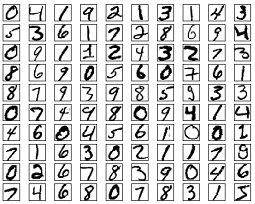
\includegraphics{mnist_100_digits.png}
\caption{Part of the so-called MNIST training sample}
\end{figure}

By increasing the number of training examples, the network can learn
more about handwriting, and so improve its accuracy. So while I've shown
just 100 training digits above, we could certainly build a better
handwriting recognizer by using thousands or even millions or billions
of training examples (\textbf{as we have seen above neural nets are not
capable of extrapolating results, hence it won't recongnize a digit
written in some strange way not included in the training sample !!!}).

Let's try to implement an ANN that is capable of recognizing handwritten
digits. To start we need to install another module, \texttt{mnist} which
containes various predefined training samples. This can be done by using
\texttt{pip}, which is a very useful tool that allows to install new
modules to your python libraries or alternatively using the Anaconda GUI
following the \emph{Environment} tab.

Our program will be based on a Convolutional Neural Network (CNN) which
is specifically designed for image/pattern recognition. We won't go in
the details since it is outside the scope of this lecture but it works
essentially by applying on top of an image a series of filters
(\emph{convolutional layers}) that works as edge detectors and with them
it classifies the images according to their relevant features.

Convolutional layers prove very effective, and stacking them in deep
models allows layers close to the input to learn low-level features
(e.g.~lines) and layers deeper in the model to learn high-order or more
abstract features, like shapes or specific objects.

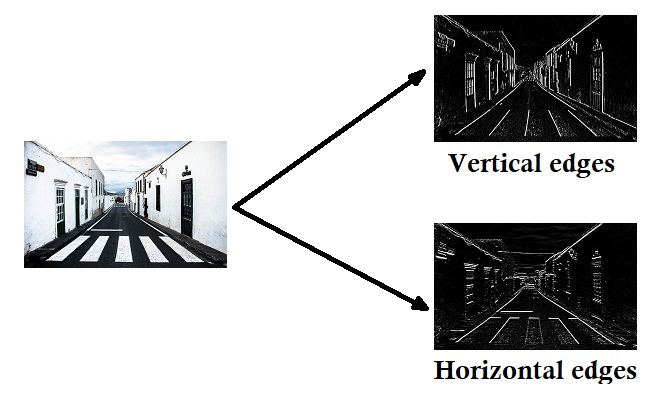
\includegraphics{edges.jpg}

Another important difference with respect to the previous examples is
that in this case we are going to solve a classification problem
(contrary to before when we were trying to regress a sample or in other
word to approximate a function). Indeed our NN output won't be a single
number but rather a vector containing the probabilties that a
handwritten digit was 0, 1, 2, \ldots{}, 8 and 9.

    \begin{tcolorbox}[breakable, size=fbox, boxrule=1pt, pad at break*=1mm,colback=cellbackground, colframe=cellborder]
\prompt{In}{incolor}{10}{\boxspacing}
\begin{Verbatim}[commandchars=\\\{\}]
\PY{k+kn}{import} \PY{n+nn}{numpy} \PY{k}{as} \PY{n+nn}{np}
\PY{c+c1}{\PYZsh{} contains our dataset for training}
\PY{k+kn}{import} \PY{n+nn}{mnist} 

\PY{k+kn}{from} \PY{n+nn}{finnn} \PY{k}{import} \PY{n}{FinNN}

\PY{c+c1}{\PYZsh{} load the training}
\PY{n}{train\PYZus{}images} \PY{o}{=} \PY{n}{mnist}\PY{o}{.}\PY{n}{train\PYZus{}images}\PY{p}{(}\PY{p}{)} \PY{c+c1}{\PYZsh{} the actual images}
\PY{n}{train\PYZus{}labels} \PY{o}{=} \PY{n}{mnist}\PY{o}{.}\PY{n}{train\PYZus{}labels}\PY{p}{(}\PY{p}{)} \PY{c+c1}{\PYZsh{} the truth (it is a 0, 1, 2...)}

\PY{c+c1}{\PYZsh{} 0 means do not split the sample in training and testing sets}
\PY{c+c1}{\PYZsh{} (MNIST has already dont it for us)}
\PY{c+c1}{\PYZsh{} the last parameter tells FinNN class that we are going to develop a CNN}
\PY{n}{trainer} \PY{o}{=} \PY{n}{FinNN}\PY{p}{(}\PY{l+s+s2}{\PYZdq{}}\PY{l+s+s2}{CNN2D}\PY{l+s+s2}{\PYZdq{}}\PY{p}{)}
\PY{n}{trainer}\PY{o}{.}\PY{n}{setData}\PY{p}{(}\PY{n}{train\PYZus{}images}\PY{p}{,} \PY{n}{train\PYZus{}labels}\PY{p}{)}

\PY{c+c1}{\PYZsh{}trainer.normalize()}
\PY{c+c1}{\PYZsh{} for technical reasons you need to expand axis}
\PY{n}{trainer}\PY{o}{.}\PY{n}{x} \PY{o}{=} \PY{n}{np}\PY{o}{.}\PY{n}{expand\PYZus{}dims}\PY{p}{(}\PY{n}{trainer}\PY{o}{.}\PY{n}{x}\PY{p}{,} \PY{n}{axis}\PY{o}{=}\PY{l+m+mi}{3}\PY{p}{)}
\end{Verbatim}
\end{tcolorbox}

    Next we define the CNN architecture.

    \begin{tcolorbox}[breakable, size=fbox, boxrule=1pt, pad at break*=1mm,colback=cellbackground, colframe=cellborder]
\prompt{In}{incolor}{11}{\boxspacing}
\begin{Verbatim}[commandchars=\\\{\}]
\PY{c+c1}{\PYZsh{} define our convolutional NN}
\PY{c+c1}{\PYZsh{} we decide to apply 8 filters to the images }
\PY{c+c1}{\PYZsh{} each with 3x3 pixels size}
\PY{c+c1}{\PYZsh{} the input images have 28x28 pixels size instead}
\PY{n}{trainer}\PY{o}{.}\PY{n}{addConv2DLayer}\PY{p}{(}\PY{l+m+mi}{8}\PY{p}{,} \PY{l+m+mi}{3}\PY{p}{,} \PY{p}{(}\PY{l+m+mi}{28}\PY{p}{,} \PY{l+m+mi}{28}\PY{p}{,} \PY{l+m+mi}{1}\PY{p}{)}\PY{p}{)}

\PY{c+c1}{\PYZsh{} the output is given by 10 neurons returning the }
\PY{c+c1}{\PYZsh{} probability that image is in each class.}
\PY{n}{trainer}\PY{o}{.}\PY{n}{addCNNOutputLayer}\PY{p}{(}\PY{l+m+mi}{10}\PY{p}{)}
        

\PY{c+c1}{\PYZsh{} adam is an algorithm to adjust the weights every cycle}
\PY{c+c1}{\PYZsh{} loss function compute the error between the prediction and the truth }
\PY{c+c1}{\PYZsh{} metrics which error to use }
\PY{n}{trainer}\PY{o}{.}\PY{n}{compileModel}\PY{p}{(}\PY{l+s+s1}{\PYZsq{}}\PY{l+s+s1}{categorical\PYZus{}crossentropy}\PY{l+s+s1}{\PYZsq{}}\PY{p}{,} \PY{l+s+s1}{\PYZsq{}}\PY{l+s+s1}{adam}\PY{l+s+s1}{\PYZsq{}}\PY{p}{)}

\PY{n}{trainer}\PY{o}{.}\PY{n}{fit}\PY{p}{(}\PY{l+m+mi}{5}\PY{p}{)}
\PY{c+c1}{\PYZsh{}validation\PYZus{}data=(test\PYZus{}images, to\PYZus{}categorical(test\PYZus{}labels)))}
    
\PY{n}{trainer}\PY{o}{.}\PY{n}{saveModel}\PY{p}{(}\PY{l+s+s1}{\PYZsq{}}\PY{l+s+s1}{digit\PYZus{}training}\PY{l+s+s1}{\PYZsq{}}\PY{p}{)}
\end{Verbatim}
\end{tcolorbox}

    \begin{Verbatim}[commandchars=\\\{\}]
Epoch 1/5
59999/59999 [==============================] - 11s 179us/step - loss: 1.8219
Epoch 2/5
59999/59999 [==============================] - 11s 179us/step - loss: 0.4252
Epoch 3/5
59999/59999 [==============================] - 11s 178us/step - loss: 0.2709
Epoch 4/5
59999/59999 [==============================] - 11s 178us/step - loss: 0.2130
Epoch 5/5
59999/59999 [==============================] - 11s 179us/step - loss: 0.1846
    \end{Verbatim}


 \begin{tcolorbox}[breakable, size=fbox, boxrule=1pt, pad at break*=1mm, colframe=cellborder]
    \hypertarget{for-the-most-curious-students}{%
\subsubsection{For the most curious
students}\label{for-the-most-curious-students}}

If you look closely to the \texttt{finnn.py} module you will notice that
I have cheated when describing the CNN architecture. In particular I
have not mentioned the \texttt{MaxPooling2D} layer, so let's clarify its
feature.

Convolutional layers in a convolutional neural network systematically
apply learned filters to input images in order to create feature maps
that summarize the presence of those features in the input.

A limitation of the feature map output of convolutional layers is that
they record the precise position of features in the input. This means
that small movements in the position of the feature in the input image
will result in a different feature map. This can happen with
re-cropping, rotation, shifting, and other minor changes to the input
image.

Imagine a program that look for car plates in pictures taken by a speed
radar, cars won't be in the same position in the frame so there may be
differences in the classification of similar (but not equal) pictures.

A common approach to address this problem from signal processing is
called \emph{down sampling}. This is where a lower resolution version of
an input signal (e.g.~the picture) is created that still contains the
large or important structural elements, without the fine detail that may
not be as useful to the task.

Down sampling can be achieved using a pooling layer.

Pooling involves selecting a pooling operation, much like a filter to be
applied to feature maps. The size of the pooling operation or filter is
smaller than the size of the feature map; specifically, it is almost
always 2×2 pixels. This means that the pooling layer will always reduce
the size of each feature map by a factor of 2, e.g.~each dimension is
halved. For example, a pooling layer applied to a feature map of 6×6 (36
pixels) will result in an output pooled feature map of 3×3 (9 pixels).

The most common pooling operation are: * Average Pooling: calculate the
average value for each patch on the feature map; * Maximum Pooling (or
Max Pooling): calculate the maximum value for each patch of the feature
map.
\end{tcolorbox}

Now let's try to see how well our NN predicts MNIST testing digits.

    \begin{tcolorbox}[breakable, size=fbox, boxrule=1pt, pad at break*=1mm,colback=cellbackground, colframe=cellborder]
\prompt{In}{incolor}{12}{\boxspacing}
\begin{Verbatim}[commandchars=\\\{\}]
\PY{k+kn}{import} \PY{n+nn}{numpy} \PY{k}{as} \PY{n+nn}{np}
\PY{k+kn}{import} \PY{n+nn}{mnist}

\PY{n}{trainer}\PY{o}{.}\PY{n}{loadModel}\PY{p}{(}\PY{l+s+s1}{\PYZsq{}}\PY{l+s+s1}{digit\PYZus{}training}\PY{l+s+s1}{\PYZsq{}}\PY{p}{)}

\PY{c+c1}{\PYZsh{} testing with mnist test sample}
\PY{n}{test\PYZus{}images} \PY{o}{=} \PY{n}{mnist}\PY{o}{.}\PY{n}{test\PYZus{}images}\PY{p}{(}\PY{p}{)}
\PY{n}{test\PYZus{}labels} \PY{o}{=} \PY{n}{mnist}\PY{o}{.}\PY{n}{test\PYZus{}labels}\PY{p}{(}\PY{p}{)}

\PY{n}{test\PYZus{}images} \PY{o}{=} \PY{n}{np}\PY{o}{.}\PY{n}{expand\PYZus{}dims}\PY{p}{(}\PY{n}{test\PYZus{}images}\PY{p}{,} \PY{n}{axis}\PY{o}{=}\PY{l+m+mi}{3}\PY{p}{)}

\PY{n}{predictions} \PY{o}{=} \PY{n}{trainer}\PY{o}{.}\PY{n}{predict}\PY{p}{(}\PY{n}{test\PYZus{}images}\PY{p}{[}\PY{p}{:}\PY{l+m+mi}{10}\PY{p}{]}\PY{p}{)}
\PY{n+nb}{print} \PY{p}{(}\PY{l+s+s2}{\PYZdq{}}\PY{l+s+s2}{Tesing on MNIST digits...}\PY{l+s+s2}{\PYZdq{}}\PY{p}{)}
\PY{n+nb}{print}\PY{p}{(}\PY{l+s+s2}{\PYZdq{}}\PY{l+s+s2}{Predicted: }\PY{l+s+s2}{\PYZdq{}}\PY{p}{,} \PY{n}{np}\PY{o}{.}\PY{n}{argmax}\PY{p}{(}\PY{n}{predictions}\PY{p}{,} \PY{n}{axis}\PY{o}{=}\PY{l+m+mi}{1}\PY{p}{)}\PY{p}{)} 
\PY{n+nb}{print}\PY{p}{(}\PY{l+s+s2}{\PYZdq{}}\PY{l+s+s2}{Truth:}\PY{l+s+s2}{\PYZdq{}}\PY{p}{,} \PY{n}{test\PYZus{}labels}\PY{p}{[}\PY{p}{:}\PY{l+m+mi}{10}\PY{p}{]}\PY{p}{)}

\PY{c+c1}{\PYZsh{} this line returns the highest probability of the vector}
\PY{n+nb}{print}\PY{p}{(}\PY{l+s+s2}{\PYZdq{}}\PY{l+s+s2}{highest prob.:}\PY{l+s+s2}{\PYZdq{}}\PY{p}{,} \PY{p}{[}\PY{l+s+s2}{\PYZdq{}}\PY{l+s+si}{\PYZob{}:.6f\PYZcb{}}\PY{l+s+s2}{\PYZdq{}}\PY{o}{.}\PY{n}{format}\PY{p}{(}\PY{n}{p}\PY{p}{[}\PY{n}{np}\PY{o}{.}\PY{n}{argmax}\PY{p}{(}\PY{n}{p}\PY{p}{)}\PY{p}{]}\PY{p}{)} \PY{k}{for} \PY{n}{p} \PY{o+ow}{in} \PY{n}{predictions}\PY{p}{]}\PY{p}{)}
\end{Verbatim}
\end{tcolorbox}

    \begin{Verbatim}[commandchars=\\\{\}]
Tesing on MNIST digits{\ldots}
Predicted:  [7 2 1 0 4 1 4 9 6 9]
Truth: [7 2 1 0 4 1 4 9 5 9]
highest prob.: ['1.000000', '1.000000', '0.999987', '0.999998', '1.000000',
'0.999993', '0.993805', '0.652628', '0.959723', '0.999988']
    \end{Verbatim}

    Since the last two digits have lower probabilites let's check the entire
vectors to see which other number have non-zero probability.

    \begin{tcolorbox}[breakable, size=fbox, boxrule=1pt, pad at break*=1mm,colback=cellbackground, colframe=cellborder]
\prompt{In}{incolor}{14}{\boxspacing}
\begin{Verbatim}[commandchars=\\\{\}]
\PY{n+nb}{print}\PY{p}{(}\PY{l+s+s2}{\PYZdq{}}\PY{l+s+s2}{8th digit:}\PY{l+s+s2}{\PYZdq{}}\PY{p}{,} \PY{p}{[}\PY{l+s+s2}{\PYZdq{}}\PY{l+s+s2}{dig }\PY{l+s+si}{\PYZob{}\PYZcb{}}\PY{l+s+s2}{: }\PY{l+s+si}{\PYZob{}:.6f\PYZcb{}}\PY{l+s+s2}{\PYZdq{}}\PY{o}{.}\PY{n}{format}\PY{p}{(}\PY{n}{i}\PY{p}{,} \PY{n}{p}\PY{p}{)} \PY{k}{for} \PY{n}{i}\PY{p}{,} \PY{n}{p} \PY{o+ow}{in} \PY{n+nb}{enumerate}\PY{p}{(}\PY{n}{predictions}\PY{p}{[}\PY{l+m+mi}{7}\PY{p}{]}\PY{p}{)}\PY{p}{]}\PY{p}{)}
\PY{n+nb}{print} \PY{p}{(}\PY{p}{)}
\PY{n+nb}{print}\PY{p}{(}\PY{l+s+s2}{\PYZdq{}}\PY{l+s+s2}{9th digit:}\PY{l+s+s2}{\PYZdq{}}\PY{p}{,} \PY{p}{[}\PY{l+s+s2}{\PYZdq{}}\PY{l+s+s2}{dig }\PY{l+s+si}{\PYZob{}\PYZcb{}}\PY{l+s+s2}{: }\PY{l+s+si}{\PYZob{}:.6f\PYZcb{}}\PY{l+s+s2}{\PYZdq{}}\PY{o}{.}\PY{n}{format}\PY{p}{(}\PY{n}{i}\PY{p}{,} \PY{n}{p}\PY{p}{)} \PY{k}{for} \PY{n}{i}\PY{p}{,} \PY{n}{p} \PY{o+ow}{in} \PY{n+nb}{enumerate}\PY{p}{(}\PY{n}{predictions}\PY{p}{[}\PY{l+m+mi}{8}\PY{p}{]}\PY{p}{)}\PY{p}{]}\PY{p}{)}
\end{Verbatim}
\end{tcolorbox}

    \begin{Verbatim}[commandchars=\\\{\}]
8th digit: ['dig 0: 0.000000', 'dig 1: 0.000000', 'dig 2: 0.000232', 'dig 3:
0.000034', 'dig 4: 0.347104', 'dig 5: 0.000001', 'dig 6: 0.000000', 'dig 7:
0.000001', 'dig 8: 0.000000', 'dig 9: 0.652628']

9th digit: ['dig 0: 0.000000', 'dig 1: 0.000000', 'dig 2: 0.000000', 'dig 3:
0.000000', 'dig 4: 0.000000', 'dig 5: 0.040277', 'dig 6: 0.959723', 'dig 7:
0.000000', 'dig 8: 0.000000', 'dig 9: 0.000000']
    \end{Verbatim}

    So in the first case the second ranked digit is 5 (which can be confused
with a six if the lower loop is almost closed), while in the second case
it is a 7 (which can be confused with a 9 if the loop is opened).

\hypertarget{exercise-8.2}{%
\subsubsection{Exercise 8.2}\label{exercise-8.2}}

To see how well our NN behaves with different kind of digits we will try
to check how it works with my calligraphy (as homework try to repeat the
exercise using your own digit following the instructions given below).

\begin{itemize}
\tightlist
\item
  Open \texttt{paint} and create a 280x280 white square
\item
  Change brush type and set the maximum size
\item
  With the mouse draw a digit
\item
  Finally save the file (e.g.~five.png)
\end{itemize}

Before passing the image to the NN it has to be resized and this is done
with an ad-hoc function (\texttt{transform\_image}) which is in the
\texttt{digit\_converter.py} module.

    \begin{tcolorbox}[breakable, size=fbox, boxrule=1pt, pad at break*=1mm,colback=cellbackground, colframe=cellborder]
\prompt{In}{incolor}{15}{\boxspacing}
\begin{Verbatim}[commandchars=\\\{\}]
\PY{k+kn}{from} \PY{n+nn}{digit\PYZus{}converter} \PY{k}{import} \PY{n}{transform\PYZus{}image}

\PY{n}{filenames} \PY{o}{=} \PY{p}{[}\PY{l+s+s1}{\PYZsq{}}\PY{l+s+s1}{four.png}\PY{l+s+s1}{\PYZsq{}}\PY{p}{,} \PY{l+s+s1}{\PYZsq{}}\PY{l+s+s1}{five.png}\PY{l+s+s1}{\PYZsq{}}\PY{p}{]}

\PY{k}{for} \PY{n}{f} \PY{o+ow}{in} \PY{n}{filenames}\PY{p}{:}
    \PY{n}{test\PYZus{}images} \PY{o}{=} \PY{n}{np}\PY{o}{.}\PY{n}{array}\PY{p}{(}\PY{n}{transform\PYZus{}image}\PY{p}{(}\PY{n}{f}\PY{p}{)}\PY{p}{)}
    \PY{n}{test\PYZus{}images} \PY{o}{=} \PY{n}{np}\PY{o}{.}\PY{n}{expand\PYZus{}dims}\PY{p}{(}\PY{n}{test\PYZus{}images}\PY{p}{,} \PY{n}{axis}\PY{o}{=}\PY{l+m+mi}{3}\PY{p}{)}

    \PY{n}{predict} \PY{o}{=} \PY{n}{trainer}\PY{o}{.}\PY{n}{predict}\PY{p}{(}\PY{n}{test\PYZus{}images}\PY{p}{)}
    \PY{n+nb}{print} \PY{p}{(}\PY{l+s+s2}{\PYZdq{}}\PY{l+s+se}{\PYZbs{}n}\PY{l+s+s2}{\PYZdq{}}\PY{p}{)}
    \PY{n+nb}{print} \PY{p}{(}\PY{l+s+s2}{\PYZdq{}}\PY{l+s+s2}{Tesing on custom digits...}\PY{l+s+s2}{\PYZdq{}}\PY{p}{)}
    \PY{n+nb}{print} \PY{p}{(}\PY{l+s+s2}{\PYZdq{}}\PY{l+s+s2}{Predicted: }\PY{l+s+s2}{\PYZdq{}}\PY{p}{,} \PY{n}{np}\PY{o}{.}\PY{n}{argmax}\PY{p}{(}\PY{n}{predict}\PY{p}{,} \PY{n}{axis}\PY{o}{=}\PY{l+m+mi}{1}\PY{p}{)}\PY{p}{)}
    \PY{n+nb}{print}\PY{p}{(}\PY{l+s+s2}{\PYZdq{}}\PY{l+s+s2}{\PYZpc{}}\PY{l+s+s2}{:}\PY{l+s+s2}{\PYZdq{}}\PY{p}{,} \PY{p}{[}\PY{l+s+s2}{\PYZdq{}}\PY{l+s+si}{\PYZob{}:.3f\PYZcb{}}\PY{l+s+s2}{\PYZdq{}}\PY{o}{.}\PY{n}{format}\PY{p}{(}\PY{n}{p}\PY{p}{[}\PY{n}{np}\PY{o}{.}\PY{n}{argmax}\PY{p}{(}\PY{n}{p}\PY{p}{)}\PY{p}{]}\PY{p}{)} \PY{k}{for} \PY{n}{p} \PY{o+ow}{in} \PY{n}{predict}\PY{p}{]}\PY{p}{)}
\end{Verbatim}
\end{tcolorbox}

    \begin{Verbatim}[commandchars=\\\{\}]
      
Tesing on custom digits{\ldots}
Predicted:  [4]
\%: ['1.000']

Tesing on custom digits{\ldots}
Predicted:  [5]
\%: ['0.999']
    \end{Verbatim}

Those the images I have checked:

\begin{figure}
  \centering
  
\includegraphics[width=0.2\linewidth]{four.png}
  
\includegraphics[width=0.2\linewidth]{five.png}
\end{figure}

    \hypertarget{technical-analysis}{%
\subsubsection{Technical Analysis}\label{technical-analysis}}

In finance, \emph{technical analysis} is a security analysis discipline
for forecasting the direction of prices through the study of past market
data, primarily price and volume. Essentially the analyst looks for
particular patterns in the price time series that are \emph{known} to
develop in predictable ways to take profit of it.

\begin{figure}
  \centering
  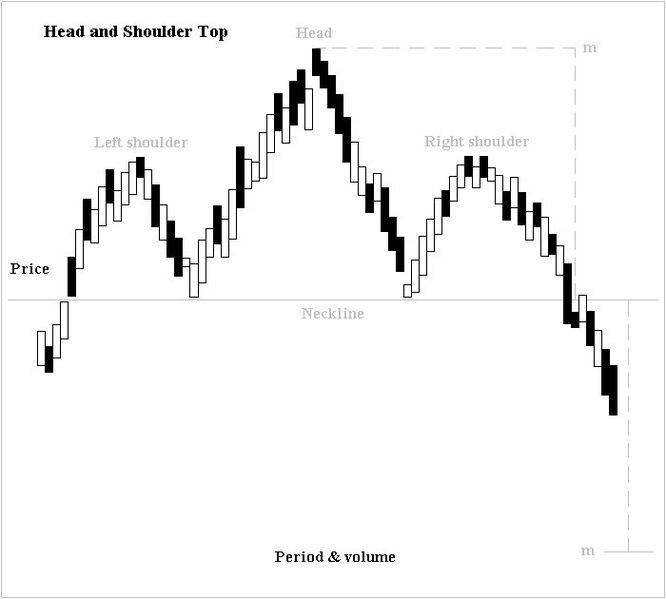
\includegraphics[width=0.4\linewidth]{H_and_s_top_new.jpg}
  
  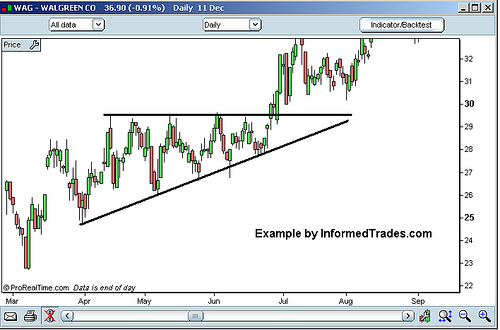
\includegraphics[width=0.4\linewidth]{Triangle-ascending.jpg}
  \caption{Examples of patterns in real time series.}
\end{figure}

As you may imagine we will try to develop a CNN (like in the handwriting
case) capable of classifying features in time series to be used in a
technical analysis (this is much faster than having somebody looking at
thousands of time series by eye\ldots{}).

I have generated myself the training set simulating 21600 time series
(1/3 with head and shoulder patter, 1/3 with triangle pattern and 1/3
with no pattern). \emph{To make the training easier the features have
been exagerated.}

\begin{figure}
  \centering
  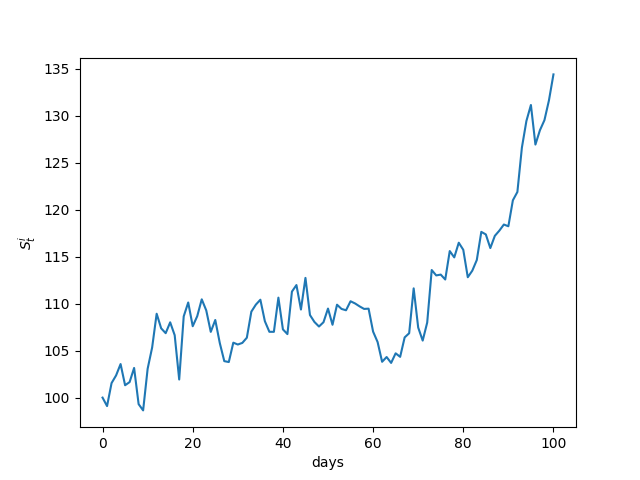
\includegraphics[width=0.6\linewidth]{image_1.png}
  \caption{An example of training image with no pattern.}
\end{figure}

\begin{figure}
  \centering
  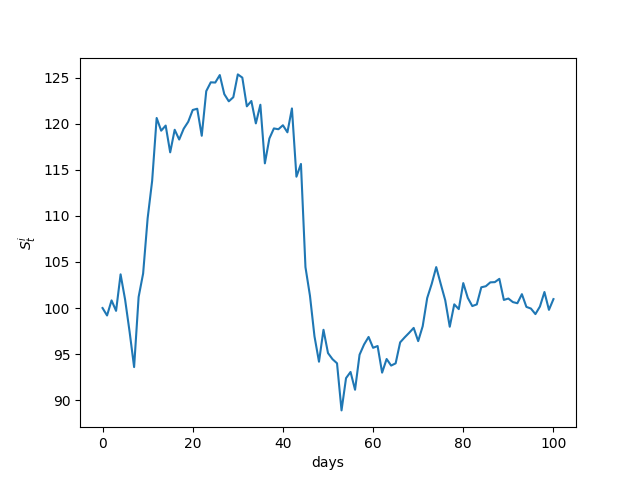
\includegraphics[width=0.6\linewidth]{image_2.png}
  \caption{An example of training image with \emph{head and shoulder} pattern.}
\end{figure}

\begin{figure}
  \centering
  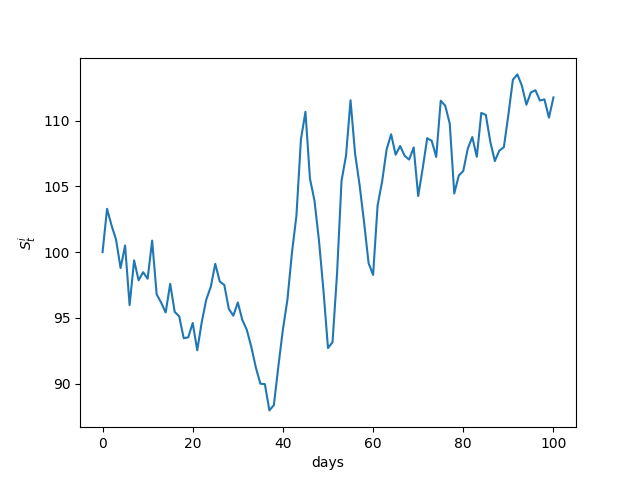
\includegraphics[width=0.6\linewidth]{image_0.png}
  \caption{An example of training image with \emph{triangle} pattern.}
\end{figure}

    \begin{tcolorbox}[breakable, size=fbox, boxrule=1pt, pad at break*=1mm,colback=cellbackground, colframe=cellborder]
\prompt{In}{incolor}{16}{\boxspacing}
\begin{Verbatim}[commandchars=\\\{\}]
\PY{k+kn}{from} \PY{n+nn}{finnn} \PY{k}{import} \PY{n}{FinNN}
\PY{k+kn}{import} \PY{n+nn}{pandas} \PY{k}{as} \PY{n+nn}{pd}
\PY{k+kn}{import} \PY{n+nn}{numpy} \PY{k}{as} \PY{n+nn}{np}

\PY{n}{train\PYZus{}labels} \PY{o}{=} \PY{n}{pd}\PY{o}{.}\PY{n}{read\PYZus{}csv}\PY{p}{(}\PY{l+s+s2}{\PYZdq{}}\PY{l+s+s2}{training\PYZus{}techana\PYZus{}labels.csv}\PY{l+s+s2}{\PYZdq{}}\PY{p}{)}
\PY{n}{train\PYZus{}images} \PY{o}{=} \PY{n}{pd}\PY{o}{.}\PY{n}{read\PYZus{}csv}\PY{p}{(}\PY{l+s+s2}{\PYZdq{}}\PY{l+s+s2}{training\PYZus{}techana\PYZus{}images.csv}\PY{l+s+s2}{\PYZdq{}}\PY{p}{)}
\PY{c+c1}{\PYZsh{}train\PYZus{}images = train\PYZus{}images[:3000]}
\PY{c+c1}{\PYZsh{}train\PYZus{}images = np.array(train\PYZus{}images)}
\PY{n}{train\PYZus{}images} \PY{o}{=} \PY{n}{np}\PY{o}{.}\PY{n}{expand\PYZus{}dims}\PY{p}{(}\PY{n}{train\PYZus{}images}\PY{p}{,} \PY{n}{axis}\PY{o}{=}\PY{l+m+mi}{2}\PY{p}{)}

\PY{n}{trainer} \PY{o}{=} \PY{n}{FinNN}\PY{p}{(}\PY{l+s+s2}{\PYZdq{}}\PY{l+s+s2}{CNN1D}\PY{l+s+s2}{\PYZdq{}}\PY{p}{)}
\PY{n}{trainer}\PY{o}{.}\PY{n}{setData}\PY{p}{(}\PY{n}{train\PYZus{}images}\PY{p}{,} \PY{n}{train\PYZus{}labels}\PY{p}{)}

\PY{c+c1}{\PYZsh{} define the CNN }
\PY{n}{trainer}\PY{o}{.}\PY{n}{addConv1DInputLayer}\PY{p}{(}\PY{l+m+mi}{80}\PY{p}{,} \PY{l+m+mi}{20}\PY{p}{,} \PY{p}{(}\PY{l+m+mi}{101}\PY{p}{,} \PY{l+m+mi}{1}\PY{p}{)}\PY{p}{)}
\PY{n}{trainer}\PY{o}{.}\PY{n}{addConv1DLayer}\PY{p}{(}\PY{l+m+mi}{80}\PY{p}{,} \PY{l+m+mi}{15}\PY{p}{)}
\PY{n}{trainer}\PY{o}{.}\PY{n}{addMaxPooling1D}\PY{p}{(}\PY{l+m+mi}{3}\PY{p}{)}
\PY{n}{trainer}\PY{o}{.}\PY{n}{addConv1DLayer}\PY{p}{(}\PY{l+m+mi}{100}\PY{p}{,} \PY{l+m+mi}{10}\PY{p}{)}
\PY{n}{trainer}\PY{o}{.}\PY{n}{addConv1DLayer}\PY{p}{(}\PY{l+m+mi}{100}\PY{p}{,} \PY{l+m+mi}{5}\PY{p}{)}
\PY{n}{trainer}\PY{o}{.}\PY{n}{addGlobalAveragePooling1D}\PY{p}{(}\PY{p}{)}
\PY{n}{trainer}\PY{o}{.}\PY{n}{addDropout}\PY{p}{(}\PY{l+m+mf}{0.5}\PY{p}{)}
\PY{n}{trainer}\PY{o}{.}\PY{n}{addCNNOutputLayer}\PY{p}{(}\PY{l+m+mi}{3}\PY{p}{)}

\PY{n}{trainer}\PY{o}{.}\PY{n}{compileModel}\PY{p}{(}\PY{l+s+s1}{\PYZsq{}}\PY{l+s+s1}{categorical\PYZus{}crossentropy}\PY{l+s+s1}{\PYZsq{}}\PY{p}{,} \PY{l+s+s1}{\PYZsq{}}\PY{l+s+s1}{adam}\PY{l+s+s1}{\PYZsq{}}\PY{p}{)}

\PY{c+c1}{\PYZsh{} make the training}
\PY{n}{trainer}\PY{o}{.}\PY{n}{fit}\PY{p}{(}\PY{l+m+mi}{80}\PY{p}{,} \PY{l+m+mi}{35}\PY{p}{)}

\PY{n}{trainer}\PY{o}{.}\PY{n}{saveModel}\PY{p}{(}\PY{l+s+s1}{\PYZsq{}}\PY{l+s+s1}{techana}\PY{l+s+s1}{\PYZsq{}}\PY{p}{)}
\end{Verbatim}
\end{tcolorbox}

    \begin{Verbatim}[commandchars=\\\{\}]
Epoch 1/80
21598/21598 [==============================] - 17s 774us/step - loss: 0.8423
...
Epoch 80/80
21598/21598 [==============================] - 17s 804us/step - loss: 0.1881
    \end{Verbatim}

 \begin{tcolorbox}[breakable, size=fbox, boxrule=1pt, pad at break*=1mm, colframe=cellborder]
    \hypertarget{again-for-the-most-curious-students}{%
\subsubsection{Again for the most curious
students}\label{again-for-the-most-curious-students}}

Large neural nets trained on relatively small datasets can overfit the
training data.

This has the effect of the model learning the statistical noise in the
training data, which results in poor performance when the model is
evaluated on new data, e.g.~a test dataset.

One approach to reduce overfitting is to fit all possible different
neural networks on the same dataset and to average the predictions from
each model. This is not feasible in practice, and can be approximated
using a small collection of different models, called an ensemble. A
problem even with the ensemble approximation is that it requires
multiple models to be fit and stored, which can be a challenge if the
models are large, requiring days or weeks to train and tune.

\emph{Dropout} is a regularization method that approximates training a
large number of neural networks with different architectures in
parallel.

During training, some number of layer outputs are randomly ignored or
\emph{dropped out}. This has the effect of making the layer look-like
and be treated-like a layer with a different number of nodes and
connectivity to the prior layer. In effect, each update to a layer
during training is performed with a different ``view'' of the configured
layer.

Even if the it may seems counterintuitive (better training when
switching off nodes) indeed dropout breaks-up situations where network
layers co-adapt to correct mistakes from prior layers, in turn making
the model more robust.
\end{tcolorbox}

To test the perfomance I wanted to simulate a real case scenario where
the time series are analyzed in real-time in order to predict as soon as
possible a particular pattern and take advantage of the prediction.

To do so I have created a longer time series and passed as input to the
CNN sliding time windows to simulate the evolution of the time series.
The goal was to check when the neural network was capable of predicting
the incoming pattern.

    \begin{tcolorbox}[breakable, size=fbox, boxrule=1pt, pad at break*=1mm,colback=cellbackground, colframe=cellborder]
\prompt{In}{incolor}{17}{\boxspacing}
\begin{Verbatim}[commandchars=\\\{\}]
\PY{k+kn}{import} \PY{n+nn}{numpy} \PY{k}{as} \PY{n+nn}{np}
\PY{k+kn}{import} \PY{n+nn}{csv}
\PY{k+kn}{from} \PY{n+nn}{keras}\PY{n+nn}{.}\PY{n+nn}{models} \PY{k}{import} \PY{n}{Sequential}\PY{p}{,} \PY{n}{load\PYZus{}model}
\PY{k+kn}{from} \PY{n+nn}{keras}\PY{n+nn}{.}\PY{n+nn}{utils} \PY{k}{import} \PY{n}{to\PYZus{}categorical}

\PY{n}{test\PYZus{}images} \PY{o}{=} \PY{n}{pd}\PY{o}{.}\PY{n}{read\PYZus{}csv}\PY{p}{(}\PY{l+s+s2}{\PYZdq{}}\PY{l+s+s2}{testing\PYZus{}techana\PYZus{}frames.csv}\PY{l+s+s2}{\PYZdq{}}\PY{p}{)}
\PY{n}{test\PYZus{}images} \PY{o}{=} \PY{n}{np}\PY{o}{.}\PY{n}{expand\PYZus{}dims}\PY{p}{(}\PY{n}{test\PYZus{}images}\PY{p}{,} \PY{n}{axis}\PY{o}{=}\PY{l+m+mi}{2}\PY{p}{)}

\PY{n}{trainer}\PY{o}{.}\PY{n}{loadModel}\PY{p}{(}\PY{l+s+s1}{\PYZsq{}}\PY{l+s+s1}{techana}\PY{l+s+s1}{\PYZsq{}}\PY{p}{)}

\PY{n}{predictions} \PY{o}{=} \PY{n}{trainer}\PY{o}{.}\PY{n}{predict}\PY{p}{(}\PY{n}{test\PYZus{}images}\PY{p}{)}
\PY{k}{for} \PY{n}{i} \PY{o+ow}{in} \PY{n+nb}{range}\PY{p}{(}\PY{n+nb}{len}\PY{p}{(}\PY{n}{predictions}\PY{p}{)}\PY{p}{)}\PY{p}{:}
    \PY{n+nb}{print} \PY{p}{(}\PY{n}{np}\PY{o}{.}\PY{n}{argmax}\PY{p}{(}\PY{n}{predictions}\PY{p}{[}\PY{n}{i}\PY{p}{]}\PY{p}{)}\PY{p}{,} \PY{p}{[}\PY{l+s+s2}{\PYZdq{}}\PY{l+s+si}{\PYZob{}:.2f\PYZcb{}}\PY{l+s+s2}{\PYZdq{}}\PY{o}{.}\PY{n}{format}\PY{p}{(}\PY{n}{p}\PY{p}{)} \PY{k}{for} \PY{n}{p} \PY{o+ow}{in} \PY{n}{predictions}\PY{p}{[}\PY{n}{i}\PY{p}{]}\PY{p}{]}\PY{p}{)}
\end{Verbatim}
\end{tcolorbox}

    \begin{Verbatim}[commandchars=\\\{\}]
0 ['0.71', '0.00', '0.29']
0 ['0.66', '0.00', '0.34']
0 ['0.82', '0.00', '0.18']
0 ['0.91', '0.00', '0.09']
2 ['0.40', '0.06', '0.54']
1 ['0.00', '1.00', '0.00']
1 ['0.00', '1.00', '0.00']
1 ['0.00', '1.00', '0.00']
1 ['0.00', '1.00', '0.00']
    \end{Verbatim}

    So at the 6th sample the CNN start recognizing the \emph{head and
shoulder} pattern in the price evolution.

    \hypertarget{exercises}{%
\subsection{Exercises}\label{exercises}}

\hypertarget{exercise-8.3}{%
\subsubsection{Exercise 8.3}\label{exercise-8.3}}

Taking as example the pricing NN trained on call, try to price put
options.


    % Add a bibliography block to the postdoc
    
    
    
\end{document}

\clearpage
\chapter{Interest Rate Swaps and Swaptions}\label{interest-rate-swaps-and-swaptions}

In the previous Chapters we have already introduces a particular type of swap, the Overnight Index Swap, here we will introduce a more general Interest Rate Swap and see how it can underlying a Swaption, the analogous of the European options for interest rate market.

\subsection{Interest Rate Swaps}\label{interest-rate-swaps}

Interest rate swaps (IRS) consist of two legs a floating and a fixed. The
contract parameters are:

\begin{itemize}
\tightlist
\item
  start date \(d_0\);
\item
  notional \(N\);
\item
  fixed rate \(K\);
\item
  floating rate tenor (months);
\item
  maturity (years).
\end{itemize}

The floating leg pays the reference LIBOR fixing at a frequency equal to
the tenor of the floating rate, so for example an IRS on a 3-month
LIBOR will pay a floating coupon every three months, an IRS on 6-month
EURIBOR pays the floating coupon every six months and so on.

The fixed leg pays a predetermined cash flow at annual frequency,
regardless of the tenor of the underlying floating rate. 

For simplicity we will only consider swaps with maturities which are multiples of 1
year.

Before going into the details of the valuation of IRSs, we need to
modify the \texttt{generate\_swap\_dates} function in our
\texttt{finmarkets} module to generate the payment dates for both the
fixed and floating legs. The modification consists of the addition of a new input
parameter, the tenor, which was previously set to 12 months.

\begin{tcolorbox}[breakable, size=fbox, boxrule=1pt, pad at break*=1mm,colback=cellbackground, colframe=cellborder]
\begin{Verbatim}[commandchars=\\\{\}]
\PY{k+kn}{from} \PY{n+nn}{datetime} \PY{k}{import} \PY{n}{date}
\PY{k+kn}{from} \PY{n+nn}{dateutil}\PY{n+nn}{.}\PY{n+nn}{relativedelta} \PY{k}{import} \PY{n}{relativedelta}
    
\PY{k}{def} \PY{n+nf}{generate\PYZus{}swap\PYZus{}dates}\PY{p}{(}\PY{n}{start\PYZus{}date}\PY{p}{,} \PY{n}{n\PYZus{}months}\PY{p}{,} \PY{n}{tenor\PYZus{}months}\PY{o}{=}\PY{l+m+mi}{12}\PY{p}{)}\PY{p}{:}
    \PY{n}{dates} \PY{o}{=} \PY{p}{[}\PY{p}{]}
    \PY{k}{for} \PY{n}{n} \PY{o+ow}{in} \PY{n+nb}{range}\PY{p}{(}\PY{l+m+mi}{0}\PY{p}{,} \PY{n}{n\PYZus{}months}\PY{p}{,} \PY{n}{tenor\PYZus{}months}\PY{p}{)}\PY{p}{:}
        \PY{n}{dates}\PY{o}{.}\PY{n}{append}\PY{p}{(}\PY{n}{start\PYZus{}date} \PY{o}{+} \PY{n}{relativedelta}\PY{p}{(}\PY{n}{months}\PY{o}{=}\PY{n}{n}\PY{p}{)}\PY{p}{)}
    \PY{n}{dates}\PY{o}{.}\PY{n}{append}\PY{p}{(}\PY{n}{start\PYZus{}date} \PY{o}{+} \PY{n}{relativedelta}\PY{p}{(}\PY{n}{months}\PY{o}{=}\PY{n}{n\PYZus{}months}\PY{p}{)}\PY{p}{)}
    \PY{k}{return} \PY{n}{dates}

\PY{n}{generate\PYZus{}swap\PYZus{}dates}\PY{p}{(}\PY{n}{date}\PY{o}{.}\PY{n}{today}\PY{p}{(}\PY{p}{)}\PY{p}{,} \PY{l+m+mi}{16}\PY{p}{,} \PY{l+m+mi}{3}\PY{p}{)}

[datetime.date(2020, 10, 15),
 datetime.date(2021, 1, 15),
 datetime.date(2021, 4, 15),
 datetime.date(2021, 7, 15),
 datetime.date(2021, 10, 15),
 datetime.date(2022, 1, 15),
 datetime.date(2022, 2, 15)]
\end{Verbatim}
\end{tcolorbox}
        
Using this function and the contract parameters we will be able to
determine a sequence of payment dates for each leg of the IRS.

\subsection{IRS Valuation}\label{irs-valuation}

Let \(d_0=d_0^{\mathrm{fixed}},...,d_p^{\mathrm{fixed}}\) be the fixed
leg payment dates and
\(d_0=d_0^{\mathrm{float}},...,d_p^{\mathrm{float}}\) be the floating
leg payment dates, and let's use the following notation:

\begin{itemize}
\tightlist
\item
  \(d\) the pricing date;
\item
  \(D(d, d')\) the discount factor observed in date \(d\) for the value
  date \(d'\);
\item
  \(F(d, d', d'')\) the forward rate observed in date \(d\) for the
  period \([d', d'']\). The rate tenor is \(\tau = d'' - d'\).
\end{itemize}

The NPV of the fixed leg is calculated as follows:

\[\mathrm{NPV}_{\mathrm{fixed}}(d; K) = N\cdot K\cdot\sum_{i=1}^{n}D(d, d_{i}^{\mathrm{fixed}})\]
while the NPV of the floating leg is calculated as follows:

\[\mathrm{NPV}_{\mathrm{float}}(d) = N\cdot\sum_{i=1}^{m}F(d, d_{j-1}^{\mathrm{float}}, d_{j}^{\mathrm{float}}) \cdot \frac{d_{j}^{\mathrm{float}}-d_{j-1}^{\mathrm{float}}}{360}
\cdot D(d, d_{i}^{\mathrm{float}})\]

Therefore the NPV of the swap (seen from the point of view of the
counter-party which receives the floating leg) is

\[\mathrm{NPV}(d; K) = \mathrm{NPV}_{\mathrm{float}}(d) - \mathrm{NPV}_{\mathrm{fixed}}(d;K)\]

For reasons which will become apparent later, it's actually more
convenient to express the NPV of an IRS as a function of the fair value
fixed rate \(S\) of the IRS, also known as the \textbf{swap rate}. \(S\)
is the value of K which makes \(\mathrm{NPV}(d)=0\).

On the basis of the previous expressions, we can easily calculate \(S\)
as:

\[\mathrm{NPV}_{\mathrm{fixed}}(d;S) = \mathrm{NPV}_{\mathrm{float}}(d)\]
\[N\cdot S\cdot\sum_{i=1}^{n}D(d, d_{i}^{\mathrm{fixed}}) = N\cdot\sum_{i=1}^{m}F(d, d_{j-1}^{\mathrm{float}}, d_{j}^{\mathrm{float}}) \cdot \frac{d_{j}^{\mathrm{float}}-d_{j-1}^{\mathrm{float}}}{360} \cdot D(d, d_{i}^{\mathrm{float}})\]
\[S=\frac{\sum_{i=1}^{m}F(d, d_{j-1}^{\mathrm{float}}, d_{j}^{\mathrm{float}}) \cdot \frac{d_{j}^{\mathrm{float}}-d_{j-1}^{\mathrm{float}}}{360}
\cdot D(d, d_{i}^{\mathrm{float}})}{\sum_{i=1}^{n}D(d, d_i^{\mathrm{fixed}})} \]

Once we have calculated \(S\), we can express the \(\mathrm{NPV}\) of an
IRS as follows:

\begin{align*}&\mathrm{NPV}(d; K) = \mathrm{NPV}_{\mathrm{float}}(d) - \mathrm{NPV}_{\mathrm{fixed}}(d; K) = & \\ \\ &= \underbrace{\mathrm{NPV}_{\mathrm{float}}(d) - \mathrm{NPV}_{\mathrm{fixed}}(d; S)}_{\mathrm{=\;0}} + \mathrm{NPV}_{\mathrm{fixed}}(d;S) - \mathrm{NPV}_{\mathrm{fixed}}(d;K) & \\ & = N\cdot(S-K)\cdot\underbrace{\sum_{i=1}^{n}D(d, d_{i}^{\mathrm{fixed}})}_{\mathrm{'annuity'}}
\end{align*}

For convenience the relevant inputs that will be used later (LIBOR and discount curve definitions) have been saved in the files \href{https://drive.google.com/file/d/1dm5oZnZKmJM6UrV0L32OcqD5Tzs9SI9A/view?usp=sharing}{libor\_curve.xlsx} and \href{https://drive.google.com/file/d/14R22r7m-6VpQ_P79D3qHdK0QN_mOQ_UB/view?usp=sharing}{discount\_curve.xlsx} respectively.

\begin{tcolorbox}[breakable, size=fbox, boxrule=1pt, pad at break*=1mm,colback=cellbackground, colframe=cellborder]
\begin{Verbatim}[commandchars=\\\{\}]
\PY{k+kn}{import} \PY{n+nn}{pandas} \PY{k}{as} \PY{n+nn}{pd}
\PY{k+kn}{from} \PY{n+nn}{datetime} \PY{k}{import} \PY{n}{date}
\PY{k+kn}{from} \PY{n+nn}{finmarkets} \PY{k}{import} \PY{n}{DiscountCurve}\PY{p}{,} \PY{n}{ForwardRateCurve}

\PY{n}{pricing\PYZus{}date} \PY{o}{=} \PY{n}{date}\PY{p}{(}\PY{l+m+mi}{2019}\PY{p}{,} \PY{l+m+mi}{11}\PY{p}{,} \PY{l+m+mi}{23}\PY{p}{)}
\PY{n}{start\PYZus{}date} \PY{o}{=} \PY{n}{date}\PY{p}{(}\PY{l+m+mi}{2021}\PY{p}{,} \PY{l+m+mi}{11}\PY{p}{,} \PY{l+m+mi}{23}\PY{p}{)}
\PY{n}{exercise\PYZus{}date} \PY{o}{=} \PY{n}{date}\PY{p}{(}\PY{l+m+mi}{2020}\PY{p}{,} \PY{l+m+mi}{11}\PY{p}{,} \PY{l+m+mi}{23}\PY{p}{)}

\PY{n}{discount\PYZus{}data} \PY{o}{=} \PY{n}{pd}\PY{o}{.}\PY{n}{read\PYZus{}excel}\PY{p}{(}\PY{l+s+s1}{\PYZsq{}}\PY{l+s+s1}{discount\PYZus{}curve.xlsx}\PY{l+s+s1}{\PYZsq{}}\PY{p}{)}
\PY{n}{libor\PYZus{}data} \PY{o}{=} \PY{n}{pd}\PY{o}{.}\PY{n}{read\PYZus{}excel}\PY{p}{(}\PY{l+s+s1}{\PYZsq{}}\PY{l+s+s1}{libor.xlsx}\PY{l+s+s1}{\PYZsq{}}\PY{p}{)}

\PY{n}{dc} \PY{o}{=} \PY{n}{DiscountCurve}\PY{p}{(}\PY{n}{pricing\PYZus{}date}\PY{p}{,} 
                   \PY{n}{discount\PYZus{}data}\PY{p}{[}\PY{l+s+s1}{\PYZsq{}}\PY{l+s+s1}{pillar}\PY{l+s+s1}{\PYZsq{}}\PY{p}{]}\PY{o}{.}\PY{n}{dt}\PY{o}{.}\PY{n}{date}\PY{o}{.}\PY{n}{tolist}\PY{p}{(}\PY{p}{)}\PY{p}{,}
                   \PY{n}{discount\PYZus{}data}\PY{p}{[}\PY{l+s+s1}{\PYZsq{}}\PY{l+s+s1}{discount\PYZus{}factor}\PY{l+s+s1}{\PYZsq{}}\PY{p}{]}\PY{o}{.}\PY{n}{tolist}\PY{p}{(}\PY{p}{)}\PY{p}{)}

\PY{n}{fr} \PY{o}{=} \PY{n}{ForwardRateCurve}\PY{p}{(}\PY{n}{libor\PYZus{}data}\PY{p}{[}\PY{l+s+s1}{\PYZsq{}}\PY{l+s+s1}{date}\PY{l+s+s1}{\PYZsq{}}\PY{p}{]}\PY{o}{.}\PY{n}{dt}\PY{o}{.}\PY{n}{date}\PY{o}{.}\PY{n}{tolist}\PY{p}{(}\PY{p}{)}\PY{p}{,}
                      \PY{n}{libor\PYZus{}data}\PY{p}{[}\PY{l+s+s1}{\PYZsq{}}\PY{l+s+s1}{rate}\PY{l+s+s1}{\PYZsq{}}\PY{p}{]}\PY{o}{.}\PY{n}{tolist}\PY{p}{(}\PY{p}{)}\PY{p}{)}

\PY{n+nb}{print}\PY{p}{(}\PY{n}{dc}\PY{o}{.}\PY{n}{df}\PY{p}{(}\PY{n}{date}\PY{p}{(}\PY{l+m+mi}{2020}\PY{p}{,} \PY{l+m+mi}{1}\PY{p}{,} \PY{l+m+mi}{1}\PY{p}{)}\PY{p}{)}\PY{p}{)}
\PY{n+nb}{print} \PY{p}{(}\PY{n}{fr}\PY{o}{.}\PY{n}{forward\PYZus{}rate}\PY{p}{(}\PY{n}{date}\PY{p}{(}\PY{l+m+mi}{2020}\PY{p}{,} \PY{l+m+mi}{1}\PY{p}{,} \PY{l+m+mi}{1}\PY{p}{)}\PY{p}{)}\PY{p}{)}

1.0003778376026249
0.01000266393442623
\end{Verbatim}
\end{tcolorbox}

Now we can implement the \texttt{InterestRateSwap} class to valuate IRS
contracts.

\begin{tcolorbox}[breakable, size=fbox, boxrule=1pt, pad at break*=1mm,colback=cellbackground, colframe=cellborder]
\begin{Verbatim}[commandchars=\\\{\}]
\PY{k}{class} \PY{n+nc}{InterestRateSwap}\PY{p}{:}    
    \PY{k}{def} \PY{n+nf}{\PYZus{}\PYZus{}init\PYZus{}\PYZus{}}\PY{p}{(}\PY{n+nb+bp}{self}\PY{p}{,} \PY{n}{start\PYZus{}date}\PY{p}{,} \PY{n}{notional}\PY{p}{,} 
                 \PY{n}{fixed\PYZus{}rate}\PY{p}{,} \PY{n}{tenor\PYZus{}months}\PY{p}{,} 
                 \PY{n}{maturity\PYZus{}years}\PY{p}{)}\PY{p}{:}
        \PY{n+nb+bp}{self}\PY{o}{.}\PY{n}{notional} \PY{o}{=} \PY{n}{notional}
        \PY{n+nb+bp}{self}\PY{o}{.}\PY{n}{fixed\PYZus{}rate} \PY{o}{=} \PY{n}{fixed\PYZus{}rate}
        \PY{n+nb+bp}{self}\PY{o}{.}\PY{n}{fixed\PYZus{}leg\PYZus{}dates} \PY{o}{=} \PYZbs{}
            \PY{n}{generate\PYZus{}swap\PYZus{}dates}\PY{p}{(}\PY{n}{start\PYZus{}date}\PY{p}{,} \PY{l+m+mi}{12} \PY{o}{*} \PY{n}{maturity\PYZus{}years}\PY{p}{)}
        \PY{n+nb+bp}{self}\PY{o}{.}\PY{n}{floating\PYZus{}leg\PYZus{}dates} \PY{o}{=} \PYZbs{}
            \PY{n}{generate\PYZus{}swap\PYZus{}dates}\PY{p}{(}\PY{n}{start\PYZus{}date}\PY{p}{,} \PY{l+m+mi}{12} \PY{o}{*} \PY{n}{maturity\PYZus{}years}\PY{p}{,}
                                \PY{n}{tenor\PYZus{}months}\PY{p}{)}
        
    \PY{k}{def} \PY{n+nf}{annuity}\PY{p}{(}\PY{n+nb+bp}{self}\PY{p}{,} \PY{n}{discount\PYZus{}curve}\PY{p}{)}\PY{p}{:}
        \PY{n}{a} \PY{o}{=} \PY{l+m+mi}{0}
        \PY{k}{for} \PY{n}{i} \PY{o+ow}{in} \PY{n+nb}{range}\PY{p}{(}\PY{l+m+mi}{1}\PY{p}{,} \PY{n+nb}{len}\PY{p}{(}\PY{n+nb+bp}{self}\PY{o}{.}\PY{n}{fixed\PYZus{}leg\PYZus{}dates}\PY{p}{)}\PY{p}{)}\PY{p}{:}
            \PY{n}{a} \PY{o}{+}\PY{o}{=} \PY{n}{discount\PYZus{}curve}\PY{o}{.}\PY{n}{df}\PY{p}{(}\PY{n+nb+bp}{self}\PY{o}{.}\PY{n}{fixed\PYZus{}leg\PYZus{}dates}\PY{p}{[}\PY{n}{i}\PY{p}{]}\PY{p}{)}
        \PY{k}{return} \PY{n}{a}

    \PY{k}{def} \PY{n+nf}{swap\PYZus{}rate}\PY{p}{(}\PY{n+nb+bp}{self}\PY{p}{,} \PY{n}{discount\PYZus{}curve}\PY{p}{,} \PY{n}{libor\PYZus{}curve}\PY{p}{)}\PY{p}{:}
        \PY{n}{s} \PY{o}{=} \PY{l+m+mi}{0}
        \PY{k}{for} \PY{n}{j} \PY{o+ow}{in} \PY{n+nb}{range}\PY{p}{(}\PY{l+m+mi}{1}\PY{p}{,} \PY{n+nb}{len}\PY{p}{(}\PY{n+nb+bp}{self}\PY{o}{.}\PY{n}{floating\PYZus{}leg\PYZus{}dates}\PY{p}{)}\PY{p}{)}\PY{p}{:}
            \PY{n}{F} \PY{o}{=} \PY{n}{libor\PYZus{}curve}\PY{o}{.}\PY{n}{forward\PYZus{}rate}\PY{p}{(}\PY{n+nb+bp}{self}\PY{o}{.}\PY{n}{floating\PYZus{}leg\PYZus{}dates}\PY{p}{[}\PY{n}{j}\PY{o}{\PYZhy{}}\PY{l+m+mi}{1}\PY{p}{]}\PY{p}{)}
            \PY{n}{tau} \PY{o}{=} \PY{p}{(}\PY{n+nb+bp}{self}\PY{o}{.}\PY{n}{floating\PYZus{}leg\PYZus{}dates}\PY{p}{[}\PY{n}{j}\PY{p}{]} \PY{o}{\PYZhy{}} \PYZbs{}
                   \PY{n+nb+bp}{self}\PY{o}{.}\PY{n}{floating\PYZus{}leg\PYZus{}dates}\PY{p}{[}\PY{n}{j}\PY{o}{\PYZhy{}}\PY{l+m+mi}{1}\PY{p}{]}\PY{p}{)}\PY{o}{.}\PY{n}{days} \PY{o}{/} \PY{l+m+mi}{360}
            \PY{n}{P} \PY{o}{=} \PY{n}{discount\PYZus{}curve}\PY{o}{.}\PY{n}{df}\PY{p}{(}\PY{n+nb+bp}{self}\PY{o}{.}\PY{n}{floating\PYZus{}leg\PYZus{}dates}\PY{p}{[}\PY{n}{j}\PY{p}{]}\PY{p}{)}
            \PY{n}{s} \PY{o}{+}\PY{o}{=} \PY{n}{F} \PY{o}{*} \PY{n}{tau} \PY{o}{*} \PY{n}{P}
        \PY{k}{return} \PY{n}{s} \PY{o}{/} \PY{n+nb+bp}{self}\PY{o}{.}\PY{n}{annuity}\PY{p}{(}\PY{n}{discount\PYZus{}curve}\PY{p}{)}
        
    \PY{k}{def} \PY{n+nf}{npv}\PY{p}{(}\PY{n+nb+bp}{self}\PY{p}{,} \PY{n}{discount\PYZus{}curve}\PY{p}{,} \PY{n}{libor\PYZus{}curve}\PY{p}{)}\PY{p}{:}
        \PY{n}{S} \PY{o}{=} \PY{n+nb+bp}{self}\PY{o}{.}\PY{n}{swap\PYZus{}rate}\PY{p}{(}\PY{n}{discount\PYZus{}curve}\PY{p}{,} \PY{n}{libor\PYZus{}curve}\PY{p}{)}
        \PY{n}{A} \PY{o}{=} \PY{n+nb+bp}{self}\PY{o}{.}\PY{n}{annuity}\PY{p}{(}\PY{n}{discount\PYZus{}curve}\PY{p}{)}
        \PY{k}{return} \PY{n+nb+bp}{self}\PY{o}{.}\PY{n}{notional} \PY{o}{*} \PY{p}{(}\PY{n}{S} \PY{o}{\PYZhy{}} \PY{n+nb+bp}{self}\PY{o}{.}\PY{n}{fixed\PYZus{}rate}\PY{p}{)} \PY{o}{*} \PY{n}{A}
\end{Verbatim}
\end{tcolorbox}

Let's test our class instantiating an IRS with 1M notional, fixed rate
of 5\%, 6 month tenor and a maturity of 4 years; discount and LIBOR
curves are the same as before.

\begin{tcolorbox}[breakable, size=fbox, boxrule=1pt, pad at break*=1mm,colback=cellbackground, colframe=cellborder]
\begin{Verbatim}[commandchars=\\\{\}]
\PY{n}{pricing\PYZus{}date} \PY{o}{=} \PY{n}{date}\PY{p}{(}\PY{l+m+mi}{2019}\PY{p}{,} \PY{l+m+mi}{11}\PY{p}{,} \PY{l+m+mi}{23}\PY{p}{)}
\PY{n}{irs} \PY{o}{=} \PY{n}{InterestRateSwap}\PY{p}{(}\PY{n}{pricing\PYZus{}date}\PY{p}{,} \PY{l+m+mf}{1e6}\PY{p}{,} \PY{l+m+mf}{0.05}\PY{p}{,} \PY{l+m+mi}{6}\PY{p}{,} \PY{l+m+mi}{4}\PY{p}{)}
\PY{n+nb}{print} \PY{p}{(}\PY{l+s+s2}{\PYZdq{}}\PY{l+s+si}{\PYZob{}:.2f\PYZcb{}}\PY{l+s+s2}{ EUR}\PY{l+s+s2}{\PYZdq{}}\PY{o}{.}\PY{n}{format}\PY{p}{(}\PY{n}{irs}\PY{o}{.}\PY{n}{npv}\PY{p}{(}\PY{n}{dc}\PY{p}{,} \PY{n}{fr}\PY{p}{)}\PY{p}{)}\PY{p}{)}

-160130.58 EUR
\end{Verbatim}
\end{tcolorbox}

\textbf{Can you guess what could be the swap rate given that the NPV is negative ?}

(Remember that we are looking at this contracts from the point of view
of the receiver of the floating leg\ldots{})

\begin{tcolorbox}[breakable, size=fbox, boxrule=1pt, pad at break*=1mm,colback=cellbackground, colframe=cellborder]
\begin{Verbatim}[commandchars=\\\{\}]
\PY{n+nb}{print} \PY{p}{(}\PY{l+s+s2}{\PYZdq{}}\PY{l+s+si}{\PYZob{}\PYZcb{}}\PY{l+s+s2}{\PYZdq{}}\PY{o}{.}\PY{n}{format}\PY{p}{(}\PY{n}{irs}\PY{o}{.}\PY{n}{swap\PYZus{}rate}\PY{p}{(}\PY{n}{dc}\PY{p}{,} \PY{n}{fr}\PY{p}{)}\PY{p}{)}\PY{p}{)}

0.010254255993254186
\end{Verbatim}
\end{tcolorbox}
    
To check if the we have computed correctly the swap rate we can
instantiate a new IRS with fixed rate equal to the just calculated swap
rate and print its NPV, it should come very close to 0.

\begin{tcolorbox}[breakable, size=fbox, boxrule=1pt, pad at break*=1mm,colback=cellbackground, colframe=cellborder]
\begin{Verbatim}[commandchars=\\\{\}]
\PY{n}{irs2} \PY{o}{=} \PY{n}{InterestRateSwap}\PY{p}{(}\PY{n}{pricing\PYZus{}date}\PY{p}{,} \PY{l+m+mf}{1e6}\PY{p}{,} \PY{l+m+mf}{0.01025425}\PY{p}{,} \PY{l+m+mi}{6}\PY{p}{,} \PY{l+m+mi}{4}\PY{p}{)}
\PY{n+nb}{print} \PY{p}{(}\PY{l+s+s2}{\PYZdq{}}\PY{l+s+si}{\PYZob{}:.2f\PYZcb{}}\PY{l+s+s2}{ EUR}\PY{l+s+s2}{\PYZdq{}}\PY{o}{.}\PY{n}{format}\PY{p}{(}\PY{n}{irs2}\PY{o}{.}\PY{n}{npv}\PY{p}{(}\PY{n}{dc}\PY{p}{,} \PY{n}{fr}\PY{p}{)}\PY{p}{)}\PY{p}{)}

0.02 EUR
\end{Verbatim}
\end{tcolorbox}
    
\section{Inheritance Again}
Now that we have introduced two kind of swaps we can try to make an alternative implementation of their classes, this time using inheritance.

The base (or parent) class will be \texttt{GenericSwap} and it will implement just the constructor taking in input the basic data characterizing a swap: notional, maturity, tenor and rate of the fixed leg. We will slightly modify the implementation of the \texttt{OvernightIndexSwap} class since now the payment dates are computed directly in the constructor of \texttt{GenericSwap}.

\begin{tcolorbox}[breakable, size=fbox, boxrule=1pt, pad at break*=1mm,colback=cellbackground, colframe=cellborder]
\begin{Verbatim}[commandchars=\\\{\}]
\PY{k}{class} \PY{n+nc}{GenericSwap}\PY{p}{:}
    \PY{k}{def} \PY{n+nf}{\PYZus{}\PYZus{}init\PYZus{}\PYZus{}}\PY{p}{(}\PY{n+nb+bp}{self}\PY{p}{,} \PY{n}{start\PYZus{}date}\PY{p}{,} \PY{n}{notional}\PY{p}{,} 
                 \PY{n}{fixed\PYZus{}rate}\PY{p}{,} \PY{n}{maturity\PYZus{}years}\PY{p}{,} \PY{n}{tenor\PYZus{}months}\PY{o}{=}\PY{l+m+mi}{12}\PY{p}{)}\PY{p}{:}
        \PY{n+nb+bp}{self}\PY{o}{.}\PY{n}{notional} \PY{o}{=} \PY{n}{notional}
        \PY{n+nb+bp}{self}\PY{o}{.}\PY{n}{fixed\PYZus{}rate} \PY{o}{=} \PY{n}{fixed\PYZus{}rate}
        \PY{n+nb+bp}{self}\PY{o}{.}\PY{n}{fixed\PYZus{}leg\PYZus{}dates} \PY{o}{=} \PYZbs{}
            \PY{n}{generate\PYZus{}swap\PYZus{}dates}\PY{p}{(}\PY{n}{start\PYZus{}date}\PY{p}{,} \PY{l+m+mi}{12} \PY{o}{*} \PY{n}{maturity\PYZus{}years}\PY{p}{)}
        \PY{n+nb+bp}{self}\PY{o}{.}\PY{n}{floating\PYZus{}leg\PYZus{}dates} \PY{o}{=} \PYZbs{}
            \PY{n}{generate\PYZus{}swap\PYZus{}dates}\PY{p}{(}\PY{n}{start\PYZus{}date}\PY{p}{,} \PY{l+m+mi}{12} \PY{o}{*} \PY{n}{maturity\PYZus{}years}\PY{p}{,} \PY{n}{tenor\PYZus{}months}\PY{p}{)}
        \PY{n+nb+bp}{self}\PY{o}{.}\PY{n}{maturity} \PY{o}{=} \PY{n}{maturity\PYZus{}years}
	
    \PY{k}{def} \PY{n+nf}{npv}\PY{p}{(}\PY{n+nb+bp}{self}\PY{p}{)}\PY{p}{:}
        \PY{n+nb}{print} \PY{p}{(}\PY{l+s+s2}{\PYZdq{}}\PY{l+s+si}{\PYZob{}\PYZcb{}}\PY{l+s+s2}{ doesn}\PY{l+s+s2}{\PYZsq{}}\PY{l+s+s2}{t implement npv method.}\PY{l+s+s2}{\PYZdq{}}\PY{o}{.}\PY{n}{format}\PY{p}{(}\PY{n+nb+bp}{self}\PY{o}{.}\PY{n+nv+vm}{\PYZus{}\PYZus{}name\PYZus{}\PYZus{}}\PY{p}{)}\PY{p}{)}
	
\PY{k}{class} \PY{n+nc}{OvernightIndexSwap}\PY{p}{(}\PY{n}{GenericSwap}\PY{p}{)}\PY{p}{:}
    \PY{k}{def} \PY{n+nf}{npv\PYZus{}floating\PYZus{}leg}\PY{p}{(}\PY{n+nb+bp}{self}\PY{p}{,} \PY{n}{discount\PYZus{}curve}\PY{p}{)}\PY{p}{:}
        \PY{k}{return} \PY{n+nb+bp}{self}\PY{o}{.}\PY{n}{notional} \PY{o}{*} \PY{p}{(}\PY{n}{discount\PYZus{}curve}\PY{o}{.}\PY{n}{df}\PY{p}{(}\PY{n+nb+bp}{self}\PY{o}{.}\PY{n}{floating\PYZus{}leg\PYZus{}dates}\PY{p}{[}\PY{l+m+mi}{0}\PY{p}{]}\PY{p}{)} \PY{o}{\PYZhy{}}
                                \PY{n}{discount\PYZus{}curve}\PY{o}{.}\PY{n}{df}\PY{p}{(}\PY{n+nb+bp}{self}\PY{o}{.}\PY{n}{floating\PYZus{}leg\PYZus{}dates}\PY{p}{[}\PY{o}{\PYZhy{}}\PY{l+m+mi}{1}\PY{p}{]}\PY{p}{)}\PY{p}{)}
	
    \PY{k}{def} \PY{n+nf}{npv\PYZus{}fixed\PYZus{}leg}\PY{p}{(}\PY{n+nb+bp}{self}\PY{p}{,} \PY{n}{discount\PYZus{}curve}\PY{p}{)}\PY{p}{:}
        \PY{n}{npv} \PY{o}{=} \PY{l+m+mi}{0}
        \PY{k}{for} \PY{n}{i} \PY{o+ow}{in} \PY{n+nb}{range}\PY{p}{(}\PY{l+m+mi}{1}\PY{p}{,} \PY{n+nb}{len}\PY{p}{(}\PY{n+nb+bp}{self}\PY{o}{.}\PY{n}{fixed\PYZus{}leg\PYZus{}dates}\PY{p}{)}\PY{p}{)}\PY{p}{:}
            \PY{n}{start\PYZus{}date} \PY{o}{=} \PY{n+nb+bp}{self}\PY{o}{.}\PY{n}{fixed\PYZus{}leg\PYZus{}dates}\PY{p}{[}\PY{n}{i}\PY{o}{\PYZhy{}}\PY{l+m+mi}{1}\PY{p}{]}
            \PY{n}{end\PYZus{}date} \PY{o}{=} \PY{n+nb+bp}{self}\PY{o}{.}\PY{n}{fixed\PYZus{}leg\PYZus{}dates}\PY{p}{[}\PY{n}{i}\PY{p}{]}
            \PY{n}{tau} \PY{o}{=} \PY{p}{(}\PY{n}{end\PYZus{}date} \PY{o}{\PYZhy{}} \PY{n}{start\PYZus{}date}\PY{p}{)}\PY{o}{.}\PY{n}{days} \PY{o}{/} \PY{l+m+mi}{360}
            \PY{n}{df} \PY{o}{=} \PY{n}{discount\PYZus{}curve}\PY{o}{.}\PY{n}{df}\PY{p}{(}\PY{n}{end\PYZus{}date}\PY{p}{)}
            \PY{n}{npv} \PY{o}{+=} \PY{n}{df} \PY{o}{*} \PY{n}{tau}
        \PY{k}{return} \PY{n+nb+bp}{self}\PY{o}{.}\PY{n}{notional} \PY{o}{*} \PY{n+nb+bp}{self}\PY{o}{.}\PY{n}{fixed\PYZus{}rate} \PY{o}{*} \PY{n}{npv}
	
    \PY{k}{def} \PY{n+nf}{npv}\PY{p}{(}\PY{n+nb+bp}{self}\PY{p}{,} \PY{n}{discount\PYZus{}curve}\PY{p}{)}\PY{p}{:}
        \PY{n}{float\PYZus{}npv} \PY{o}{=} \PY{n+nb+bp}{self}\PY{o}{.}\PY{n}{npv\PYZus{}floating\PYZus{}leg}\PY{p}{(}\PY{n}{discount\PYZus{}curve}\PY{p}{)}
        \PY{n}{fixed\PYZus{}npv} \PY{o}{=} \PY{n+nb+bp}{self}\PY{o}{.}\PY{n}{npv\PYZus{}fixed\PYZus{}leg}\PY{p}{(}\PY{n}{discount\PYZus{}curve}\PY{p}{)}
        \PY{k}{return} \PY{n}{float\PYZus{}npv} \PY{o}{\PYZhy{}} \PY{n}{fixed\PYZus{}npv}
	
\PY{k}{class} \PY{n+nc}{InterestRateSwap}\PY{p}{(}\PY{n}{GenericSwap}\PY{p}{)}\PY{p}{:}        
    \PY{k}{def} \PY{n+nf}{annuity}\PY{p}{(}\PY{n+nb+bp}{self}\PY{p}{,} \PY{n}{discount\PYZus{}curve}\PY{p}{)}\PY{p}{:}
        \PY{n}{a} \PY{o}{=} \PY{l+m+mi}{0}
        \PY{k}{for} \PY{n}{i} \PY{o+ow}{in} \PY{n+nb}{range}\PY{p}{(}\PY{l+m+mi}{1}\PY{p}{,} \PY{n+nb}{len}\PY{p}{(}\PY{n+nb+bp}{self}\PY{o}{.}\PY{n}{fixed\PYZus{}leg\PYZus{}dates}\PY{p}{)}\PY{p}{)}\PY{p}{:}
            \PY{n}{a} \PY{o}{+}\PY{o}{=} \PY{n}{discount\PYZus{}curve}\PY{o}{.}\PY{n}{df}\PY{p}{(}\PY{n+nb+bp}{self}\PY{o}{.}\PY{n}{fixed\PYZus{}leg\PYZus{}dates}\PY{p}{[}\PY{n}{i}\PY{p}{]}\PY{p}{)}
        \PY{k}{return} \PY{n}{a}
	
    \PY{k}{def} \PY{n+nf}{swap\PYZus{}rate}\PY{p}{(}\PY{n+nb+bp}{self}\PY{p}{,} \PY{n}{discount\PYZus{}curve}\PY{p}{,} \PY{n}{libor\PYZus{}curve}\PY{p}{)}\PY{p}{:}
        \PY{n}{s} \PY{o}{=} \PY{l+m+mi}{0}
        \PY{k}{for} \PY{n}{j} \PY{o+ow}{in} \PY{n+nb}{range}\PY{p}{(}\PY{l+m+mi}{1}\PY{p}{,} \PY{n+nb}{len}\PY{p}{(}\PY{n+nb+bp}{self}\PY{o}{.}\PY{n}{floating\PYZus{}leg\PYZus{}dates}\PY{p}{)}\PY{p}{)}\PY{p}{:}
            \PY{n}{F} \PY{o}{=} \PY{n}{libor\PYZus{}curve}\PY{o}{.}\PY{n}{forward\PYZus{}rate}\PY{p}{(}\PY{n+nb+bp}{self}\PY{o}{.}\PY{n}{floating\PYZus{}leg\PYZus{}dates}\PY{p}{[}\PY{n}{j}\PY{o}{\PYZhy{}}\PY{l+m+mi}{1}\PY{p}{]}\PY{p}{)}
            \PY{n}{tau} \PY{o}{=} \PY{p}{(}\PY{n+nb+bp}{self}\PY{o}{.}\PY{n}{floating\PYZus{}leg\PYZus{}dates}\PY{p}{[}\PY{n}{j}\PY{p}{]} \PY{o}{\PYZhy{}} \PYZbs{}
            \PY{n+nb+bp}{self}\PY{o}{.}\PY{n}{floating\PYZus{}leg\PYZus{}dates}\PY{p}{[}\PY{n}{j}\PY{o}{\PYZhy{}}\PY{l+m+mi}{1}\PY{p}{]}\PY{p}{)}\PY{o}{.}\PY{n}{days} \PY{o}{/} \PY{l+m+mi}{360}
            \PY{n}{P} \PY{o}{=} \PY{n}{discount\PYZus{}curve}\PY{o}{.}\PY{n}{df}\PY{p}{(}\PY{n+nb+bp}{self}\PY{o}{.}\PY{n}{floating\PYZus{}leg\PYZus{}dates}\PY{p}{[}\PY{n}{j}\PY{p}{]}\PY{p}{)}
            \PY{n}{s} \PY{o}{+}\PY{o}{=} \PY{n}{F} \PY{o}{*} \PY{n}{tau} \PY{o}{*} \PY{n}{P}
        \PY{k}{return} \PY{n}{s} \PY{o}{/} \PY{n+nb+bp}{self}\PY{o}{.}\PY{n}{annuity}\PY{p}{(}\PY{n}{discount\PYZus{}curve}\PY{p}{)}
	
    \PY{k}{def} \PY{n+nf}{npv}\PY{p}{(}\PY{n+nb+bp}{self}\PY{p}{,} \PY{n}{discount\PYZus{}curve}\PY{p}{,} \PY{n}{libor\PYZus{}curve}\PY{p}{)}\PY{p}{:}
        \PY{n}{S} \PY{o}{=} \PY{n+nb+bp}{self}\PY{o}{.}\PY{n}{swap\PYZus{}rate}\PY{p}{(}\PY{n}{discount\PYZus{}curve}\PY{p}{,} \PY{n}{libor\PYZus{}curve}\PY{p}{)}
        \PY{n}{A} \PY{o}{=} \PY{n+nb+bp}{self}\PY{o}{.}\PY{n}{annuity}\PY{p}{(}\PY{n}{discount\PYZus{}curve}\PY{p}{)}
        \PY{k}{return} \PY{n+nb+bp}{self}\PY{o}{.}\PY{n}{notional} \PY{o}{*} \PY{p}{(}\PY{n}{S} \PY{o}{\PYZhy{}} \PY{n+nb+bp}{self}\PY{o}{.}\PY{n}{fixed\PYZus{}rate}\PY{p}{)} \PY{o}{*} \PY{n}{A}
\end{Verbatim}
\end{tcolorbox}

This is just an example. Actually may be an overkill to use inheritance here, since there is not much of code to share between the classes (the implementation of the NPV calculation is different in each of them).
Anyway this is a practical application to show how it works.

\section{Swaptions}\label{interest-rate-swaptions}

Swaptions are the equivalent of European options for the interest rate
markets. They give the option holder the right but not the obligation,
at the exercise date \(d_{ex}\), to enter into an Interest Rate Swap at
a pre-determined fixed rate.

Clearly the option holder will only choose to do this if the NPV of the
underlying swap at \(d_{ex}\) is positive - looking at the expression
for the NPV of the IRS in terms of the swap rate \(S\) therefore, we can
see that the payoff of the swaption is

\[N\cdot \mathrm{max}(0, S(d_{\mathrm{ex}}) - K)\cdot\sum D(d_{\mathrm{ex}}, d_i^{\mathrm{fixed}})\]

The key issue is now to estimate \(S(d_{\mathrm{ex}})\) in order to
evaluate the payoff of a swaption. This will be shown with two
alternative approaches.

\subsection{Evaluation through Black-Scholes Formula}\label{evaluation-through-black-scholes-formula}

In this case, to evaluate the NPV of this payoff, we'll use a
generalization of the Black-Scholes-Merton formula applied to swaptions:

\[\mathrm{NPV} = N\cdot A\cdot [S \mathcal{N}(d_+) - K\mathcal{N}(d_-)]\]
where \(\mathcal{N}\) represent a normal distribution

\[d_{\pm} = \frac{\mathrm{log}(\frac{S}{K}) \pm \frac{1}{2}\sigma^{2}T}{\sigma\sqrt{T}}\qquad(\sigma~\textrm{is the volatility of the swap rate})\\\]
\[A =\sum_{i=1}^{p}D(d, d_{i}^{\mathrm{fixed}})\qquad\mathrm{(annuity})\]

As an example let's consider a swaption whose underlying 6M-IRS has a
notional of 1M, fixed rate of 1\%, and a maturity of 4 years. In
addition we assume a volatility associated to the swap rate of about
7\%.

\begin{tcolorbox}[breakable, size=fbox, boxrule=1pt, pad at break*=1mm,colback=cellbackground, colframe=cellborder]
\begin{Verbatim}[commandchars=\\\{\}]
\PY{k+kn}{from} \PY{n+nn}{math} \PY{k}{import} \PY{n}{log}
\PY{k+kn}{from} \PY{n+nn}{scipy}\PY{n+nn}{.}\PY{n+nn}{stats} \PY{k}{import} \PY{n}{norm} 
\PY{k+kn}{from} \PY{n+nn}{dateutil}\PY{n+nn}{.}\PY{n+nn}{relativedelta} \PY{k}{import} \PY{n}{relativedelta}

\PY{k}{def} \PY{n+nf}{npvSwaptionBS}\PY{p}{(}\PY{n}{irs}\PY{p}{,} \PY{n}{sigma}\PY{p}{,} 
                  \PY{n}{pricing\PYZus{}date}\PY{p}{,}
                  \PY{n}{exercise\PYZus{}date}\PY{p}{,} 
                  \PY{n}{discount\PYZus{}curve}\PY{p}{,} \PY{n}{libor\PYZus{}curve}\PY{p}{)}\PY{p}{:}
    \PY{n}{T} \PY{o}{=} \PY{p}{(}\PY{n}{exercise\PYZus{}date} \PY{o}{\PYZhy{}} \PY{n}{pricing\PYZus{}date}\PY{p}{)}\PY{o}{.}\PY{n}{days} \PY{o}{/} \PY{l+m+mi}{365}
    \PY{n}{A} \PY{o}{=} \PY{n}{irs}\PY{o}{.}\PY{n}{annuity}\PY{p}{(}\PY{n}{discount\PYZus{}curve}\PY{p}{)}
    \PY{n}{S} \PY{o}{=} \PY{n}{irs}\PY{o}{.}\PY{n}{swap\PYZus{}rate}\PY{p}{(}\PY{n}{discount\PYZus{}curve}\PY{p}{,} \PY{n}{libor\PYZus{}curve}\PY{p}{)}
    \PY{n}{K} \PY{o}{=} \PY{n}{irs}\PY{o}{.}\PY{n}{fixed\PYZus{}rate}
    \PY{n}{N} \PY{o}{=} \PY{n}{irs}\PY{o}{.}\PY{n}{notional}
    
    \PY{n}{d\PYZus{}plus} \PY{o}{=} \PY{p}{(}\PY{n}{log}\PY{p}{(}\PY{n}{S}\PY{o}{/}\PY{n}{K}\PY{p}{)} \PY{o}{+} \PY{l+m+mf}{0.5} \PY{o}{*} \PY{n}{sigma}\PY{o}{*}\PY{o}{*}\PY{l+m+mi}{2} \PY{o}{*} \PY{n}{T}\PY{p}{)} \PY{o}{/} \PY{p}{(}\PY{n}{sigma} \PY{o}{*} \PY{n}{T}\PY{o}{*}\PY{o}{*}\PY{l+m+mf}{0.5}\PY{p}{)}
    \PY{n}{d\PYZus{}minus} \PY{o}{=} \PY{p}{(}\PY{n}{log}\PY{p}{(}\PY{n}{S}\PY{o}{/}\PY{n}{K}\PY{p}{)} \PY{o}{\PYZhy{}} \PY{l+m+mf}{0.5} \PY{o}{*} \PY{n}{sigma}\PY{o}{*}\PY{o}{*}\PY{l+m+mi}{2} \PY{o}{*} \PY{n}{T}\PY{p}{)} \PY{o}{/} \PY{p}{(}\PY{n}{sigma} \PY{o}{*} \PY{n}{T}\PY{o}{*}\PY{o}{*}\PY{l+m+mf}{0.5}\PY{p}{)}
    \PY{k}{return} \PY{n}{irs}\PY{o}{.}\PY{n}{notional} \PY{o}{*} \PY{n}{A} \PY{o}{*} \PY{p}{(}\PY{n}{S} \PY{o}{*} \PY{n}{norm}\PY{o}{.}\PY{n}{cdf}\PY{p}{(}\PY{n}{d\PYZus{}plus}\PY{p}{)} \PY{o}{\PYZhy{}} \PY{n}{K} \PY{o}{*} \PY{n}{norm}\PY{o}{.}\PY{n}{cdf}\PY{p}{(}\PY{n}{d\PYZus{}minus}\PY{p}{)}\PY{p}{)}

\PY{n}{sigma} \PY{o}{=} \PY{l+m+mf}{0.07}
\PY{n}{irs} \PY{o}{=} \PY{n}{InterestRateSwap}\PY{p}{(}\PY{n}{pricing\PYZus{}date}\PY{p}{,} \PY{l+m+mf}{1e6}\PY{p}{,} \PY{l+m+mf}{0.01}\PY{p}{,} \PY{l+m+mi}{6}\PY{p}{,} \PY{l+m+mi}{4}\PY{p}{)}
\PY{n}{exercise\PYZus{}date} \PY{o}{=} \PY{n}{start\PYZus{}date} \PY{o}{+} \PY{n}{relativedelta}\PY{p}{(}\PY{n}{years}\PY{o}{=}\PY{l+m+mi}{4}\PY{p}{)}

\PY{n}{npv} \PY{o}{=} \PY{n}{npvSwaptionBS}\PY{p}{(}\PY{n}{irs}\PY{p}{,} \PY{n}{sigma}\PY{p}{,} \PY{n}{pricing\PYZus{}date}\PY{p}{,} 
                    \PY{n}{exercise\PYZus{}date}\PY{p}{,} \PY{n}{dc}\PY{p}{,} \PY{n}{fr}\PY{p}{)}
\PY{n+nb}{print}\PY{p}{(}\PY{l+s+s2}{\PYZdq{}}\PY{l+s+s2}{Swaption NPV with BS: }\PY{l+s+si}{\PYZob{}:.3f\PYZcb{}}\PY{l+s+s2}{ EUR}\PY{l+s+s2}{\PYZdq{}}\PY{o}{.}\PY{n}{format}\PY{p}{(}\PY{n}{npv}\PY{p}{)}\PY{p}{)}

Swaption NPV with BS: 3330.741 EUR
\end{Verbatim}
\end{tcolorbox}

\paragraph{Evaluation through Monte-Carlo Simulation}\label{evaluation-through-monte-carlo-simulation}

In this second case we start from the current swap rate \(S(d)\)
evaluated at the pricing date \(d\), and assume that it follows a
log-normal stochastic process, i.e. its distribution at
\(d_{\mathrm{ex}}\) (exercise date) is
\(S(d_{\mathrm{ex}}) = S(d)\mathrm{exp}(-\frac{1}{2}\sigma^{2}T+\sigma\sqrt{T}\epsilon)\)
where \(\epsilon\approx\mathcal{N}(0,1)\). Notice that it is assumed
that the \emph{drift} rate in the evolution of the swap rate is zero.
Given that the discounted payoff is given by:

\[N\cdot \mathrm{max}(0, S(d_{\mathrm{ex}}) - K)\cdot\sum D(d_{\mathrm{ex}}, d_i^{\mathrm{fixed}})\]
to perform the simulation we can:

\begin{itemize}
\tightlist
\item
  sample the normal distribution \(\mathcal{N}(0, 1)\) to calculate a
  large number of scenarios for \(S(d_{\mathrm{ex}})\);
\item
  evaluate the underlying swap's NPV at the expiry date, and
  consequently the swaption's payoff, for each scenario;
\item
  take the average of these values to get the final estimate.
\end{itemize}

\begin{tcolorbox}[breakable, size=fbox, boxrule=1pt, pad at break*=1mm,colback=cellbackground, colframe=cellborder]
\begin{Verbatim}[commandchars=\\\{\}]
\PY{k+kn}{import} \PY{n+nn}{numpy} \PY{k}{as} \PY{n+nn}{np}
\PY{k+kn}{from} \PY{n+nn}{math} \PY{k}{import} \PY{n}{exp}\PY{p}{,} \PY{n}{sqrt}
\PY{k+kn}{from} \PY{n+nn}{numpy}\PY{n+nn}{.}\PY{n+nn}{random} \PY{k}{import} \PY{n}{normal}\PY{p}{,} \PY{n}{seed}

\PY{c+c1}{\PYZsh{} define the number of Monte Carlo scenarios}
\PY{n}{n\PYZus{}scenarios} \PY{o}{=} \PY{l+m+mi}{50000}
\PY{n}{discounted\PYZus{}payoffs} \PY{o}{=} \PY{p}{[}\PY{p}{]}
\PY{n}{seed}\PY{p}{(}\PY{l+m+mi}{1}\PY{p}{)}

\PY{n}{T} \PY{o}{=} \PY{p}{(}\PY{n}{exercise\PYZus{}date} \PY{o}{\PYZhy{}} \PY{n}{pricing\PYZus{}date}\PY{p}{)}\PY{o}{.}\PY{n}{days} \PY{o}{/} \PY{l+m+mi}{365}
\PY{n}{A} \PY{o}{=} \PY{n}{irs}\PY{o}{.}\PY{n}{annuity}\PY{p}{(}\PY{n}{dc}\PY{p}{)}
\PY{n}{S} \PY{o}{=} \PY{n}{irs}\PY{o}{.}\PY{n}{swap\PYZus{}rate}\PY{p}{(}\PY{n}{dc}\PY{p}{,} \PY{n}{fr}\PY{p}{)}
    
\PY{k}{for} \PY{n}{i\PYZus{}scenario} \PY{o+ow}{in} \PY{n+nb}{range}\PY{p}{(}\PY{n}{n\PYZus{}scenarios}\PY{p}{)}\PY{p}{:}
    \PY{n}{S\PYZus{}simulated} \PY{o}{=} \PY{n}{S} \PY{o}{*} \PY{n}{exp}\PY{p}{(}\PY{o}{\PYZhy{}}\PY{l+m+mf}{0.5} \PY{o}{*} \PY{n}{sigma} \PY{o}{*} \PY{n}{sigma} \PY{o}{*} \PY{n}{T} \PY{o}{+}
                          \PY{n}{sigma} \PY{o}{*} \PY{n}{sqrt}\PY{p}{(}\PY{n}{T}\PY{p}{)} \PY{o}{*} \PY{n}{normal}\PY{p}{(}\PY{p}{)}\PY{p}{)}
    
    \PY{c+c1}{\PYZsh{} calculate the swap NPV in this scenario}
    \PY{n}{swap\PYZus{}npv} \PY{o}{=} \PY{n}{irs}\PY{o}{.}\PY{n}{notional} \PY{o}{*} \PY{p}{(}\PY{n}{S\PYZus{}simulated} \PY{o}{\PYZhy{}} \PY{n}{irs}\PY{o}{.}\PY{n}{fixed\PYZus{}rate}\PY{p}{)} \PY{o}{*} \PY{n}{A}
    
    \PY{c+c1}{\PYZsh{} add the discounted payoff of the swaption, in this scenario, to the list}
    \PY{n}{discounted\PYZus{}payoffs}\PY{o}{.}\PY{n}{append}\PY{p}{(}\PY{n+nb}{max}\PY{p}{(}\PY{l+m+mi}{0}\PY{p}{,} \PY{n}{swap\PYZus{}npv}\PY{p}{)}\PY{p}{)}
    
\PY{c+c1}{\PYZsh{} calculate the NPV of the swaption }
\PY{c+c1}{\PYZsh{} by taking the average of the discounted }
\PY{c+c1}{\PYZsh{} payoffs across all the scenarios}
\PY{n}{npv\PYZus{}mc} \PY{o}{=} \PY{n}{np}\PY{o}{.}\PY{n}{mean}\PY{p}{(}\PY{n}{discounted\PYZus{}payoffs}\PY{p}{)}
\PY{n+nb}{print}\PY{p}{(}\PY{l+s+s2}{\PYZdq{}}\PY{l+s+s2}{Swaption NPV: }\PY{l+s+si}{\PYZob{}:.2f\PYZcb{}}\PY{l+s+s2}{ EUR}\PY{l+s+s2}{\PYZdq{}}\PY{o}{.}\PY{n}{format}\PY{p}{(}\PY{n}{npv\PYZus{}mc}\PY{p}{)}\PY{p}{)}

Swaption NPV: 3351.42 EUR
\end{Verbatim}
\end{tcolorbox}

Note that this is not \emph{strictly speaking} the correct way of
calculating the swaption NPV, the reason being that one should calculate
the swap NPV at the expiry date of the swaption, apply the payoff
function max(0, \ldots{}) and \emph{then} discount from the expiry date
to today.

However, it's simpler to calculate it as above and it doesn't make any
difference for the result, since

\[ DF\cdot \mathrm{max}(0, \mathrm{SwapNPVAtExpiry}) = \mathrm{max}(0, DF \cdot\mathrm{SwapNPVAtExpiry}) \]

\subsection{Confidence interval}\label{confidence-interval}

By the \href{https://en.wikipedia.org/wiki/Central_limit_theorem}{central limit theorem} we know that 

\[ \hat{\mu}_n = \frac{1}{n}\sum_{i=1}^{n}Y_i\]
is approximately distributed like a normal distribution around the true value $\mu$ and variance $\sigma^2 /n$ ($\mathcal{N}(\mu ,\sigma^2 /n)$). 
This means
that if ones repeats the swaption MC experiment (e.g.~changing the seed
of the random number generator) she would obtain results normally
distributed around the the \emph{true} value \(\mu\), see Fig.~\ref{fig:repeated_MC}
The higher is \(n\) the narrower is the distribution of the results
around \(\mu\).

\begin{figure}[htb]
	\centering
	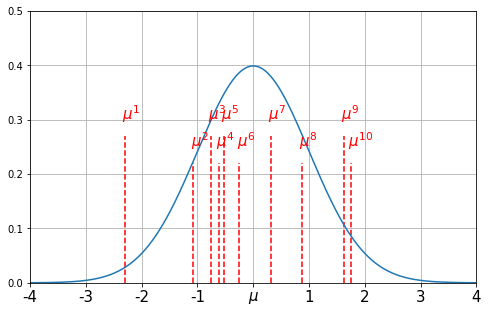
\includegraphics[width=0.7\textwidth]{lesson4_files/lesson4_33_0.png}
	\caption{Distribution of a series of ten Monte Carlo experiments around the \emph{true} value $\mu$.}
	\label{fig:repeated_MC}
\end{figure}

Therefore \( \hat{\mu}_n - \mu \) is approximately distributed as 
\[ \hat{\mu}_n - \mu \approx \frac{\sigma}{\sqrt{n}}Z \]
where $Z=\mathcal{N}(0, 1)$ is the standard Gaussian.

This means that given a Monte Carlo experiment the true value $\mu$ will lay in the interval $\hat{\mu}_n \pm  \frac{\sigma}{\sqrt{n}}Z$ around our best estimate. 
\begin{figure}[h]
	\centering
	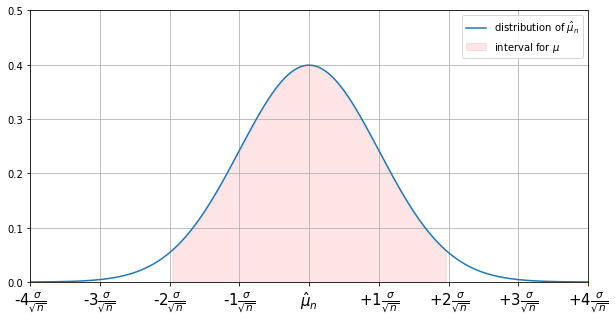
\includegraphics[width=0.7\textwidth]{confidence_interval.png}
	\caption{Confidence interval graphical explanation.}
	\label{fig:confidence}
\end{figure}
Referring to Fig.~\ref{fig:confidence} we can write:
\[\mathbb{P}\Big(\hat{\mu}_n - \frac{1.96\sigma}{\sqrt{n}} \le \mu \le \hat{\mu}_n + \frac{1.96\sigma}{\sqrt{n}}\Big) = 0.95 \]
which corresponds to the shaded area.

The interval above is called 95\% \textbf{confidence interval}. If a variable $X$ is distributed as a Gaussian $\mathcal{N}(\mu, \sigma^2)$ then
\[\mathbb{P}(\mu - 1.96\sigma \le X \le \mu+ 1.96\sigma) = 0.95 \]
because the interval $\pm 1.96\sigma$ covers 95\% of the total area under the Gaussian, in formula $\Phi(1.96)=0.975$ where $\Phi$ is the Gaussian cumulative distribution function.

To construct a confidence interval with a confidence level $\alpha$ different from 0.95, we have to find a number $A$ such that
\begin{equation}
	\Phi(A) = 1 - \frac{1-\alpha}{2}\quad\implies\quad A = \Phi^{-1}\left(\cfrac{1+\alpha}{2}\right)
	\label{for:A}
\end{equation}
then the $\alpha$-confidence interval
\[\mathbb{P}(\mu - A\sigma \le X \le \mu+ A\sigma) = \alpha \]

The width of the confidence interval is a measure of the accuracy of our estimate.
$\alpha$-confidence interval can be expressed in terms of repeated
experiments like the following: if you repeat many time a simulation,
the fraction of calculated confidence intervals (which would differ for each sample) that contains
the true parameter would tend toward $\alpha \%$ (beware! anyway in $1-\alpha\%$ of cases it is outside the interval!).

Below an example of how to compute a confidence level in \texttt{python} given a set of fake simulations. To note that the inverse of the Gaussian CDF $\Phi^{-1}$, used in Equation~\ref{for:A}, is computed with the method \texttt{norm.ppf()} (more details on CDF in Chapter~\ref{quantile-function}).

\begin{tcolorbox}[breakable, size=fbox, boxrule=1pt, pad at break*=1mm,colback=cellbackground, colframe=cellborder]
\begin{Verbatim}[commandchars=\\\{\}]
\PY{k+kn}{import} \PY{n+nn}{numpy} \PY{k}{as} \PY{n+nn}{np}
\PY{k+kn}{from} \PY{n+nn}{scipy}\PY{n+nn}{.}\PY{n+nn}{stats} \PY{k}{import} \PY{n}{norm}
		
\PY{n}{samples} \PY{o}{=} \PY{p}{[}\PY{l+m+mf}{1.}\PY{p}{,}\PY{l+m+mf}{2.}\PY{p}{,}\PY{l+m+mf}{3.}\PY{p}{,}\PY{l+m+mf}{4.}\PY{p}{,}\PY{l+m+mf}{4.}\PY{p}{,}\PY{l+m+mf}{4.}\PY{p}{,}\PY{l+m+mf}{5.}\PY{p}{,}\PY{l+m+mf}{5.}\PY{p}{,}\PY{l+m+mf}{5.}\PY{p}{,}\PY{l+m+mf}{5.}\PY{p}{,}\PY{l+m+mf}{4.}\PY{p}{,}\PY{l+m+mf}{4.}\PY{p}{,}\PY{l+m+mf}{4.}\PY{p}{,}\PY{l+m+mf}{6.}\PY{p}{,}\PY{l+m+mf}{7.}\PY{p}{,}\PY{l+m+mf}{8.}\PY{p}{]}
\PY{n}{alpha} \PY{o}{=} \PY{l+m+mf}{0.95}
		
\PY{n}{X} \PY{o}{=} \PY{n}{np}\PY{o}{.}\PY{n}{array}\PY{p}{(}\PY{n}{samples}\PY{p}{)}
\PY{n}{A} \PY{o}{=} \PY{n}{norm}\PY{o}{.}\PY{n}{ppf}\PY{p}{(}\PY{p}{(}\PY{l+m+mi}{1} \PY{o}{+} \PY{n}{alpha}\PY{p}{)}\PY{o}{/}\PY{l+m+mi}{2}\PY{p}{)}
\PY{n}{m}\PY{p}{,} \PY{n}{se} \PY{o}{=} \PY{n}{np}\PY{o}{.}\PY{n}{mean}\PY{p}{(}\PY{n}{X}\PY{p}{)}\PY{p}{,} \PY{n}{np}\PY{o}{.}\PY{n}{std}\PY{p}{(}\PY{n}{X}\PY{p}{)}
\PY{n}{h} \PY{o}{=} \PY{n}{A}\PY{o}{*}\PY{n}{se}\PY{o}{/}\PY{n}{np}\PY{o}{.}\PY{n}{sqrt}\PY{p}{(}\PY{n+nb}{len}\PY{p}{(}\PY{n}{samples}\PY{p}{)}\PY{p}{)}
\PY{n+nb}{print} \PY{p}{(}\PY{l+s+s2}{\PYZdq{}}\PY{l+s+si}{\PYZob{}:.0f\PYZcb{}}\PY{l+s+si}{\PYZpc{} c}\PY{l+s+s2}{onfidence interval: }\PY{l+s+si}{\PYZob{}\PYZcb{}}\PY{l+s+s2}{ +\PYZhy{} }\PY{l+s+si}{\PYZob{}\PYZcb{}}\PY{l+s+s2}{\PYZdq{}}\PY{o}{.}\PY{n}{format}\PY{p}{(}\PY{n}{alpha}\PY{o}{*}\PY{l+m+mi}{100}\PY{p}{,} \PY{n}{m}\PY{p}{,} \PY{n}{h}\PY{p}{)}\PY{p}{)}
		
95\% confidence interval: 4.4375 +- 0.8119808363806419
\end{Verbatim}
\end{tcolorbox}

Let's calculate the 95\% confidence level for the swaption simulation above.

\begin{tcolorbox}[breakable, size=fbox, boxrule=1pt, pad at break*=1mm,colback=cellbackground, colframe=cellborder]
\begin{Verbatim}[commandchars=\\\{\}]
\PY{n}{npv\PYZus{}error} \PY{o}{=} \PY{l+m+mf}{1.96} \PY{o}{*} \PY{n}{np}\PY{o}{.}\PY{n}{std}\PY{p}{(}\PY{n}{discounted\PYZus{}payoffs}\PY{p}{)}\PY{o}{/}\PY{n}{sqrt}\PY{p}{(}\PY{n}{n\PYZus{}scenarios}\PY{p}{)}
				
\PY{n+nb}{print}\PY{p}{(}\PY{l+s+s2}{\PYZdq{}}\PY{l+s+s2}{Swaption NPV: }\PY{l+s+si}{\PYZob{}:.2f\PYZcb{}}\PY{l+s+s2}{ EUR (+/- }\PY{l+s+si}{\PYZob{}:.2f\PYZcb{}}\PY{l+s+s2}{ EUR with 95}\PY{l+s+si}{\PYZpc{} c}\PY{l+s+s2}{onfidence)}\PY{l+s+s2}{\PYZdq{}}\PYZbs{}
      \PY{o}{.}\PY{n}{format}\PY{p}{(}\PY{n}{npv\PYZus{}mc}\PY{p}{,} \PY{n}{npv\PYZus{}error}\PY{p}{)}\PY{p}{)}

Swaption NPV: 3351.42 EUR (+/- 74.06 EUR with 95\% confidence)
\end{Verbatim}
\end{tcolorbox}

At this point we can check if the two estimated of the swaption payoff
are compatible. The NPV calculated via the Black-Scholes-Merton formula
falls within the confidence interval produced by the Monte Carlo
simulation, so we can assert that the two methods are in agreement:

\begin{itemize}
\tightlist
\item
  Swaption NPV (BS): \euro{3330.74}
\item
  Swaption NPV (MC): \euro{3351.42}
\end{itemize}

\clearpage

% Default to the notebook output style

    


% Inherit from the specified cell style.




    
\documentclass[11pt]{article}

    
    
    \usepackage[T1]{fontenc}
    % Nicer default font (+ math font) than Computer Modern for most use cases
    \usepackage{mathpazo}

    % Basic figure setup, for now with no caption control since it's done
    % automatically by Pandoc (which extracts ![](path) syntax from Markdown).
    \usepackage{graphicx}
    % We will generate all images so they have a width \maxwidth. This means
    % that they will get their normal width if they fit onto the page, but
    % are scaled down if they would overflow the margins.
    \makeatletter
    \def\maxwidth{\ifdim\Gin@nat@width>\linewidth\linewidth
    \else\Gin@nat@width\fi}
    \makeatother
    \let\Oldincludegraphics\includegraphics
    % Set max figure width to be 80% of text width, for now hardcoded.
  
    % Ensure that by default, figures have no caption (until we provide a
    % proper Figure object with a Caption API and a way to capture that
    % in the conversion process - todo).
    \usepackage{caption}
    \DeclareCaptionLabelFormat{nolabel}{}
    \captionsetup{labelformat=nolabel}

    \usepackage{adjustbox} % Used to constrain images to a maximum size 
    \usepackage{xcolor} % Allow colors to be defined
    \usepackage{enumerate} % Needed for markdown enumerations to work
    \usepackage{geometry} % Used to adjust the document margins
    \usepackage{amsmath} % Equations
    \usepackage{amssymb} % Equations
    \usepackage{textcomp} % defines textquotesingle
    % Hack from http://tex.stackexchange.com/a/47451/13684:
    \AtBeginDocument{%
        \def\PYZsq{\textquotesingle}% Upright quotes in Pygmentized code
    }
    \usepackage{upquote} % Upright quotes for verbatim code
    \usepackage{eurosym} % defines \euro
    \usepackage[mathletters]{ucs} % Extended unicode (utf-8) support
    \usepackage[utf8x]{inputenc} % Allow utf-8 characters in the tex document
    \usepackage{fancyvrb} % verbatim replacement that allows latex
    \usepackage{grffile} % extends the file name processing of package graphics 
                         % to support a larger range 
    % The hyperref package gives us a pdf with properly built
    % internal navigation ('pdf bookmarks' for the table of contents,
    % internal cross-reference links, web links for URLs, etc.)
    \usepackage{hyperref}
    \usepackage{longtable} % longtable support required by pandoc >1.10
    \usepackage{booktabs}  % table support for pandoc > 1.12.2
    \usepackage[inline]{enumitem} % IRkernel/repr support (it uses the enumerate* environment)
    \usepackage[normalem]{ulem} % ulem is needed to support strikethroughs (\sout)
                                % normalem makes italics be italics, not underlines
    \usepackage{mathrsfs}
    

    
    
    % Colors for the hyperref package
    \definecolor{urlcolor}{rgb}{0,.145,.698}
    \definecolor{linkcolor}{rgb}{.71,0.21,0.01}
    \definecolor{citecolor}{rgb}{.12,.54,.11}

    % ANSI colors
    \definecolor{ansi-black}{HTML}{3E424D}
    \definecolor{ansi-black-intense}{HTML}{282C36}
    \definecolor{ansi-red}{HTML}{E75C58}
    \definecolor{ansi-red-intense}{HTML}{B22B31}
    \definecolor{ansi-green}{HTML}{00A250}
    \definecolor{ansi-green-intense}{HTML}{007427}
    \definecolor{ansi-yellow}{HTML}{DDB62B}
    \definecolor{ansi-yellow-intense}{HTML}{B27D12}
    \definecolor{ansi-blue}{HTML}{208FFB}
    \definecolor{ansi-blue-intense}{HTML}{0065CA}
    \definecolor{ansi-magenta}{HTML}{D160C4}
    \definecolor{ansi-magenta-intense}{HTML}{A03196}
    \definecolor{ansi-cyan}{HTML}{60C6C8}
    \definecolor{ansi-cyan-intense}{HTML}{258F8F}
    \definecolor{ansi-white}{HTML}{C5C1B4}
    \definecolor{ansi-white-intense}{HTML}{A1A6B2}
    \definecolor{ansi-default-inverse-fg}{HTML}{FFFFFF}
    \definecolor{ansi-default-inverse-bg}{HTML}{000000}

    % commands and environments needed by pandoc snippets
    % extracted from the output of `pandoc -s`
    \providecommand{\tightlist}{%
      \setlength{\itemsep}{0pt}\setlength{\parskip}{0pt}}
    \DefineVerbatimEnvironment{Highlighting}{Verbatim}{commandchars=\\\{\}}
    % Add ',fontsize=\small' for more characters per line
    \newenvironment{Shaded}{}{}
    \newcommand{\KeywordTok}[1]{\textcolor[rgb]{0.00,0.44,0.13}{\textbf{{#1}}}}
    \newcommand{\DataTypeTok}[1]{\textcolor[rgb]{0.56,0.13,0.00}{{#1}}}
    \newcommand{\DecValTok}[1]{\textcolor[rgb]{0.25,0.63,0.44}{{#1}}}
    \newcommand{\BaseNTok}[1]{\textcolor[rgb]{0.25,0.63,0.44}{{#1}}}
    \newcommand{\FloatTok}[1]{\textcolor[rgb]{0.25,0.63,0.44}{{#1}}}
    \newcommand{\CharTok}[1]{\textcolor[rgb]{0.25,0.44,0.63}{{#1}}}
    \newcommand{\StringTok}[1]{\textcolor[rgb]{0.25,0.44,0.63}{{#1}}}
    \newcommand{\CommentTok}[1]{\textcolor[rgb]{0.38,0.63,0.69}{\textit{{#1}}}}
    \newcommand{\OtherTok}[1]{\textcolor[rgb]{0.00,0.44,0.13}{{#1}}}
    \newcommand{\AlertTok}[1]{\textcolor[rgb]{1.00,0.00,0.00}{\textbf{{#1}}}}
    \newcommand{\FunctionTok}[1]{\textcolor[rgb]{0.02,0.16,0.49}{{#1}}}
    \newcommand{\RegionMarkerTok}[1]{{#1}}
    \newcommand{\ErrorTok}[1]{\textcolor[rgb]{1.00,0.00,0.00}{\textbf{{#1}}}}
    \newcommand{\NormalTok}[1]{{#1}}
    
    % Additional commands for more recent versions of Pandoc
    \newcommand{\ConstantTok}[1]{\textcolor[rgb]{0.53,0.00,0.00}{{#1}}}
    \newcommand{\SpecialCharTok}[1]{\textcolor[rgb]{0.25,0.44,0.63}{{#1}}}
    \newcommand{\VerbatimStringTok}[1]{\textcolor[rgb]{0.25,0.44,0.63}{{#1}}}
    \newcommand{\SpecialStringTok}[1]{\textcolor[rgb]{0.73,0.40,0.53}{{#1}}}
    \newcommand{\ImportTok}[1]{{#1}}
    \newcommand{\DocumentationTok}[1]{\textcolor[rgb]{0.73,0.13,0.13}{\textit{{#1}}}}
    \newcommand{\AnnotationTok}[1]{\textcolor[rgb]{0.38,0.63,0.69}{\textbf{\textit{{#1}}}}}
    \newcommand{\CommentVarTok}[1]{\textcolor[rgb]{0.38,0.63,0.69}{\textbf{\textit{{#1}}}}}
    \newcommand{\VariableTok}[1]{\textcolor[rgb]{0.10,0.09,0.49}{{#1}}}
    \newcommand{\ControlFlowTok}[1]{\textcolor[rgb]{0.00,0.44,0.13}{\textbf{{#1}}}}
    \newcommand{\OperatorTok}[1]{\textcolor[rgb]{0.40,0.40,0.40}{{#1}}}
    \newcommand{\BuiltInTok}[1]{{#1}}
    \newcommand{\ExtensionTok}[1]{{#1}}
    \newcommand{\PreprocessorTok}[1]{\textcolor[rgb]{0.74,0.48,0.00}{{#1}}}
    \newcommand{\AttributeTok}[1]{\textcolor[rgb]{0.49,0.56,0.16}{{#1}}}
    \newcommand{\InformationTok}[1]{\textcolor[rgb]{0.38,0.63,0.69}{\textbf{\textit{{#1}}}}}
    \newcommand{\WarningTok}[1]{\textcolor[rgb]{0.38,0.63,0.69}{\textbf{\textit{{#1}}}}}
    
    
    % Define a nice break command that doesn't care if a line doesn't already
    % exist.
    \def\br{\hspace*{\fill} \\* }
    % Math Jax compatibility definitions
    \def\gt{>}
    \def\lt{<}
    \let\Oldtex\TeX
    \let\Oldlatex\LaTeX
    \renewcommand{\TeX}{\textrm{\Oldtex}}
    \renewcommand{\LaTeX}{\textrm{\Oldlatex}}
    % Document parameters
    % Document title
    \title{lecture\_10}
    
    
    
    
    

    % Pygments definitions
    
\makeatletter
\def\PY@reset{\let\PY@it=\relax \let\PY@bf=\relax%
    \let\PY@ul=\relax \let\PY@tc=\relax%
    \let\PY@bc=\relax \let\PY@ff=\relax}
\def\PY@tok#1{\csname PY@tok@#1\endcsname}
\def\PY@toks#1+{\ifx\relax#1\empty\else%
    \PY@tok{#1}\expandafter\PY@toks\fi}
\def\PY@do#1{\PY@bc{\PY@tc{\PY@ul{%
    \PY@it{\PY@bf{\PY@ff{#1}}}}}}}
\def\PY#1#2{\PY@reset\PY@toks#1+\relax+\PY@do{#2}}

\expandafter\def\csname PY@tok@w\endcsname{\def\PY@tc##1{\textcolor[rgb]{0.73,0.73,0.73}{##1}}}
\expandafter\def\csname PY@tok@c\endcsname{\let\PY@it=\textit\def\PY@tc##1{\textcolor[rgb]{0.25,0.50,0.50}{##1}}}
\expandafter\def\csname PY@tok@cp\endcsname{\def\PY@tc##1{\textcolor[rgb]{0.74,0.48,0.00}{##1}}}
\expandafter\def\csname PY@tok@k\endcsname{\let\PY@bf=\textbf\def\PY@tc##1{\textcolor[rgb]{0.00,0.50,0.00}{##1}}}
\expandafter\def\csname PY@tok@kp\endcsname{\def\PY@tc##1{\textcolor[rgb]{0.00,0.50,0.00}{##1}}}
\expandafter\def\csname PY@tok@kt\endcsname{\def\PY@tc##1{\textcolor[rgb]{0.69,0.00,0.25}{##1}}}
\expandafter\def\csname PY@tok@o\endcsname{\def\PY@tc##1{\textcolor[rgb]{0.40,0.40,0.40}{##1}}}
\expandafter\def\csname PY@tok@ow\endcsname{\let\PY@bf=\textbf\def\PY@tc##1{\textcolor[rgb]{0.67,0.13,1.00}{##1}}}
\expandafter\def\csname PY@tok@nb\endcsname{\def\PY@tc##1{\textcolor[rgb]{0.00,0.50,0.00}{##1}}}
\expandafter\def\csname PY@tok@nf\endcsname{\def\PY@tc##1{\textcolor[rgb]{0.00,0.00,1.00}{##1}}}
\expandafter\def\csname PY@tok@nc\endcsname{\let\PY@bf=\textbf\def\PY@tc##1{\textcolor[rgb]{0.00,0.00,1.00}{##1}}}
\expandafter\def\csname PY@tok@nn\endcsname{\let\PY@bf=\textbf\def\PY@tc##1{\textcolor[rgb]{0.00,0.00,1.00}{##1}}}
\expandafter\def\csname PY@tok@ne\endcsname{\let\PY@bf=\textbf\def\PY@tc##1{\textcolor[rgb]{0.82,0.25,0.23}{##1}}}
\expandafter\def\csname PY@tok@nv\endcsname{\def\PY@tc##1{\textcolor[rgb]{0.10,0.09,0.49}{##1}}}
\expandafter\def\csname PY@tok@no\endcsname{\def\PY@tc##1{\textcolor[rgb]{0.53,0.00,0.00}{##1}}}
\expandafter\def\csname PY@tok@nl\endcsname{\def\PY@tc##1{\textcolor[rgb]{0.63,0.63,0.00}{##1}}}
\expandafter\def\csname PY@tok@ni\endcsname{\let\PY@bf=\textbf\def\PY@tc##1{\textcolor[rgb]{0.60,0.60,0.60}{##1}}}
\expandafter\def\csname PY@tok@na\endcsname{\def\PY@tc##1{\textcolor[rgb]{0.49,0.56,0.16}{##1}}}
\expandafter\def\csname PY@tok@nt\endcsname{\let\PY@bf=\textbf\def\PY@tc##1{\textcolor[rgb]{0.00,0.50,0.00}{##1}}}
\expandafter\def\csname PY@tok@nd\endcsname{\def\PY@tc##1{\textcolor[rgb]{0.67,0.13,1.00}{##1}}}
\expandafter\def\csname PY@tok@s\endcsname{\def\PY@tc##1{\textcolor[rgb]{0.73,0.13,0.13}{##1}}}
\expandafter\def\csname PY@tok@sd\endcsname{\let\PY@it=\textit\def\PY@tc##1{\textcolor[rgb]{0.73,0.13,0.13}{##1}}}
\expandafter\def\csname PY@tok@si\endcsname{\let\PY@bf=\textbf\def\PY@tc##1{\textcolor[rgb]{0.73,0.40,0.53}{##1}}}
\expandafter\def\csname PY@tok@se\endcsname{\let\PY@bf=\textbf\def\PY@tc##1{\textcolor[rgb]{0.73,0.40,0.13}{##1}}}
\expandafter\def\csname PY@tok@sr\endcsname{\def\PY@tc##1{\textcolor[rgb]{0.73,0.40,0.53}{##1}}}
\expandafter\def\csname PY@tok@ss\endcsname{\def\PY@tc##1{\textcolor[rgb]{0.10,0.09,0.49}{##1}}}
\expandafter\def\csname PY@tok@sx\endcsname{\def\PY@tc##1{\textcolor[rgb]{0.00,0.50,0.00}{##1}}}
\expandafter\def\csname PY@tok@m\endcsname{\def\PY@tc##1{\textcolor[rgb]{0.40,0.40,0.40}{##1}}}
\expandafter\def\csname PY@tok@gh\endcsname{\let\PY@bf=\textbf\def\PY@tc##1{\textcolor[rgb]{0.00,0.00,0.50}{##1}}}
\expandafter\def\csname PY@tok@gu\endcsname{\let\PY@bf=\textbf\def\PY@tc##1{\textcolor[rgb]{0.50,0.00,0.50}{##1}}}
\expandafter\def\csname PY@tok@gd\endcsname{\def\PY@tc##1{\textcolor[rgb]{0.63,0.00,0.00}{##1}}}
\expandafter\def\csname PY@tok@gi\endcsname{\def\PY@tc##1{\textcolor[rgb]{0.00,0.63,0.00}{##1}}}
\expandafter\def\csname PY@tok@gr\endcsname{\def\PY@tc##1{\textcolor[rgb]{1.00,0.00,0.00}{##1}}}
\expandafter\def\csname PY@tok@ge\endcsname{\let\PY@it=\textit}
\expandafter\def\csname PY@tok@gs\endcsname{\let\PY@bf=\textbf}
\expandafter\def\csname PY@tok@gp\endcsname{\let\PY@bf=\textbf\def\PY@tc##1{\textcolor[rgb]{0.00,0.00,0.50}{##1}}}
\expandafter\def\csname PY@tok@go\endcsname{\def\PY@tc##1{\textcolor[rgb]{0.53,0.53,0.53}{##1}}}
\expandafter\def\csname PY@tok@gt\endcsname{\def\PY@tc##1{\textcolor[rgb]{0.00,0.27,0.87}{##1}}}
\expandafter\def\csname PY@tok@err\endcsname{\def\PY@bc##1{\setlength{\fboxsep}{0pt}\fcolorbox[rgb]{1.00,0.00,0.00}{1,1,1}{\strut ##1}}}
\expandafter\def\csname PY@tok@kc\endcsname{\let\PY@bf=\textbf\def\PY@tc##1{\textcolor[rgb]{0.00,0.50,0.00}{##1}}}
\expandafter\def\csname PY@tok@kd\endcsname{\let\PY@bf=\textbf\def\PY@tc##1{\textcolor[rgb]{0.00,0.50,0.00}{##1}}}
\expandafter\def\csname PY@tok@kn\endcsname{\let\PY@bf=\textbf\def\PY@tc##1{\textcolor[rgb]{0.00,0.50,0.00}{##1}}}
\expandafter\def\csname PY@tok@kr\endcsname{\let\PY@bf=\textbf\def\PY@tc##1{\textcolor[rgb]{0.00,0.50,0.00}{##1}}}
\expandafter\def\csname PY@tok@bp\endcsname{\def\PY@tc##1{\textcolor[rgb]{0.00,0.50,0.00}{##1}}}
\expandafter\def\csname PY@tok@fm\endcsname{\def\PY@tc##1{\textcolor[rgb]{0.00,0.00,1.00}{##1}}}
\expandafter\def\csname PY@tok@vc\endcsname{\def\PY@tc##1{\textcolor[rgb]{0.10,0.09,0.49}{##1}}}
\expandafter\def\csname PY@tok@vg\endcsname{\def\PY@tc##1{\textcolor[rgb]{0.10,0.09,0.49}{##1}}}
\expandafter\def\csname PY@tok@vi\endcsname{\def\PY@tc##1{\textcolor[rgb]{0.10,0.09,0.49}{##1}}}
\expandafter\def\csname PY@tok@vm\endcsname{\def\PY@tc##1{\textcolor[rgb]{0.10,0.09,0.49}{##1}}}
\expandafter\def\csname PY@tok@sa\endcsname{\def\PY@tc##1{\textcolor[rgb]{0.73,0.13,0.13}{##1}}}
\expandafter\def\csname PY@tok@sb\endcsname{\def\PY@tc##1{\textcolor[rgb]{0.73,0.13,0.13}{##1}}}
\expandafter\def\csname PY@tok@sc\endcsname{\def\PY@tc##1{\textcolor[rgb]{0.73,0.13,0.13}{##1}}}
\expandafter\def\csname PY@tok@dl\endcsname{\def\PY@tc##1{\textcolor[rgb]{0.73,0.13,0.13}{##1}}}
\expandafter\def\csname PY@tok@s2\endcsname{\def\PY@tc##1{\textcolor[rgb]{0.73,0.13,0.13}{##1}}}
\expandafter\def\csname PY@tok@sh\endcsname{\def\PY@tc##1{\textcolor[rgb]{0.73,0.13,0.13}{##1}}}
\expandafter\def\csname PY@tok@s1\endcsname{\def\PY@tc##1{\textcolor[rgb]{0.73,0.13,0.13}{##1}}}
\expandafter\def\csname PY@tok@mb\endcsname{\def\PY@tc##1{\textcolor[rgb]{0.40,0.40,0.40}{##1}}}
\expandafter\def\csname PY@tok@mf\endcsname{\def\PY@tc##1{\textcolor[rgb]{0.40,0.40,0.40}{##1}}}
\expandafter\def\csname PY@tok@mh\endcsname{\def\PY@tc##1{\textcolor[rgb]{0.40,0.40,0.40}{##1}}}
\expandafter\def\csname PY@tok@mi\endcsname{\def\PY@tc##1{\textcolor[rgb]{0.40,0.40,0.40}{##1}}}
\expandafter\def\csname PY@tok@il\endcsname{\def\PY@tc##1{\textcolor[rgb]{0.40,0.40,0.40}{##1}}}
\expandafter\def\csname PY@tok@mo\endcsname{\def\PY@tc##1{\textcolor[rgb]{0.40,0.40,0.40}{##1}}}
\expandafter\def\csname PY@tok@ch\endcsname{\let\PY@it=\textit\def\PY@tc##1{\textcolor[rgb]{0.25,0.50,0.50}{##1}}}
\expandafter\def\csname PY@tok@cm\endcsname{\let\PY@it=\textit\def\PY@tc##1{\textcolor[rgb]{0.25,0.50,0.50}{##1}}}
\expandafter\def\csname PY@tok@cpf\endcsname{\let\PY@it=\textit\def\PY@tc##1{\textcolor[rgb]{0.25,0.50,0.50}{##1}}}
\expandafter\def\csname PY@tok@c1\endcsname{\let\PY@it=\textit\def\PY@tc##1{\textcolor[rgb]{0.25,0.50,0.50}{##1}}}
\expandafter\def\csname PY@tok@cs\endcsname{\let\PY@it=\textit\def\PY@tc##1{\textcolor[rgb]{0.25,0.50,0.50}{##1}}}

\def\PYZbs{\char`\\}
\def\PYZus{\char`\_}
\def\PYZob{\char`\{}
\def\PYZcb{\char`\}}
\def\PYZca{\char`\^}
\def\PYZam{\char`\&}
\def\PYZlt{\char`\<}
\def\PYZgt{\char`\>}
\def\PYZsh{\char`\#}
\def\PYZpc{\char`\%}
\def\PYZdl{\char`\$}
\def\PYZhy{\char`\-}
\def\PYZsq{\char`\'}
\def\PYZdq{\char`\"}
\def\PYZti{\char`\~}
% for compatibility with earlier versions
\def\PYZat{@}
\def\PYZlb{[}
\def\PYZrb{]}
\makeatother


    % Exact colors from NB
    \definecolor{incolor}{rgb}{0.0, 0.0, 0.5}
    \definecolor{outcolor}{rgb}{0.545, 0.0, 0.0}



    
    % Prevent overflowing lines due to hard-to-break entities
    \sloppy 
    % Setup hyperref package
    \hypersetup{
      breaklinks=true,  % so long urls are correctly broken across lines
      colorlinks=true,
      urlcolor=urlcolor,
      linkcolor=linkcolor,
      citecolor=citecolor,
      }
    % Slightly bigger margins than the latex defaults
    
    \geometry{verbose,tmargin=1in,bmargin=1in,lmargin=1in,rmargin=1in}
    
    

    \begin{document}
    
    
    \maketitle
    
    

    
    \hypertarget{neural-network---practical-lesson-10}{%
\section{Neural Network - Practical Lesson
10}\label{neural-network---practical-lesson-10}}

\hypertarget{overview}{%
\subsection{Overview}\label{overview}}

In this lesson we will see how machine learning techniques can be
successfully applied to solve financial problems. We will first do a
quick tour on the theory behind neural networks and then we will see an
example and two practical applications: regression and classification.

\hypertarget{neural-networks}{%
\subsection{Neural networks}\label{neural-networks}}

\hypertarget{definition}{%
\subsubsection{Definition}\label{definition}}

Artificial Neural Networks (ANN) are information processing models that
are developed by inspiring from the working principles of human brain.
Their most essential property is the ability of learning from sample
sets. The basic process units of ANN architecture are neurons which are
internally in connection with other neurons.

\begin{figure}
\centering
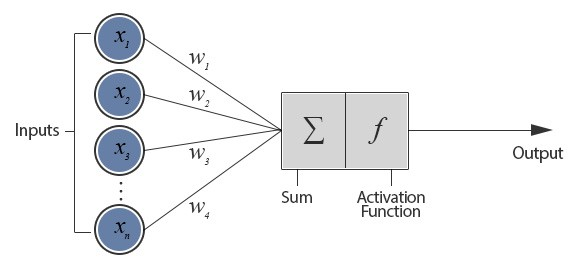
\includegraphics[width=0.8\textwidth]{neuron.jpeg}
\caption{Model of an artificial neuron.}
\end{figure}

A neuron (or more generally a perceptron) consists of weights (\(w_i\))
and real (\(x_i\)) numbers. All the inputs are individually weighted,
added together and passed into the activation function. There are many
different types of activation function but one of the simplest would be
step function (another is the sigmoid).

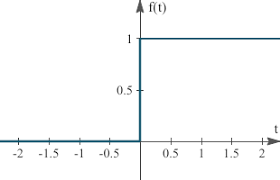
\includegraphics[width=0.45\textwidth]{step_function.png} 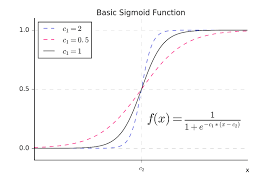
\includegraphics[width=0.45\textwidth]{sigmoid.png}

\hypertarget{training-of-perceptrons}{%
\subsubsection{Training of perceptrons}\label{training-of-perceptrons}}

When teaching children how to recognize a bus, we just tell them,
showing an example: ``This is a bus. That is not a bus.'' until they
learn the concept of what a bus is. Furthermore, if the child sees new
objects that she hasn't seen before, we could expect her to recognize
correctly whether the new object is a bus or not. This is exactly the
idea behind the perceptron. Similarly, inputs from a \emph{training} set
are presented to the perceptron one after the other and weights are
modified according to the expected output.

When an entire pass through all of the input training vectors is
completed the perceptron has learnt ! At this time, if an input vector P
(already in the training set) is given to the perceptron, it will output
the correct value. If P is not in the training set, the network will
respond with an output similar to other training vectors close to P.

Unfortunately using just a perceptron is not too useful since it is not
possible to solve the interesting problems we would like to face. The
next step is then to put together more perceptron together in
\emph{layers}.

\hypertarget{multi-layered-neural-networks}{%
\subsubsection{Multi-layered neural
networks}\label{multi-layered-neural-networks}}

\begin{figure}
\centering
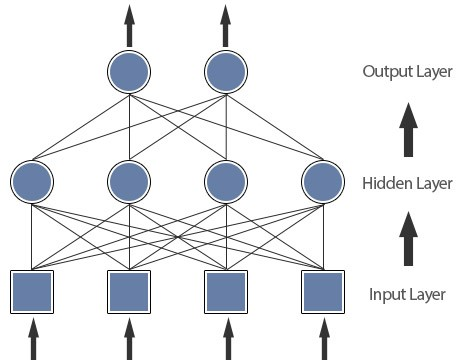
\includegraphics[width=0.8\textwidth]{multilayer.jpeg}
\caption{A multi-layered neural network.}
\end{figure}

Each input from the \emph{input layer} is fed up to each node in the
hidden layer, and from there to each node on the output layer. We should
note that there can be any number of nodes per layer and there are
usually multiple hidden layers to pass through before ultimately
reaching the output layer. But to train this network we need a learning
algorithm which should be able to tune not only the weights between the
output layer and the hidden layer but also the weights between the
hidden layer and the input layer.

\hypertarget{back-propagation}{%
\subsubsection{Back propagation}\label{back-propagation}}

First of all, we need to understand what do we lack. To tune the weights
between the hidden layer and the input layer, we need to know the error
at the hidden layer, but we know the error only at the output layer (We
know the correct output from the training sample and we also know the
output predicted by the network.) So, the method that was suggested was
to take the errors at the output layer and proportionally propagate them
backwards to the hidden layer.

So, what we are doing is:

\begin{itemize}
\tightlist
\item
  We present a training sample to the neural network (initialised with
  random weights)
\item
  Compute the output received by calculating activations of each layer
  and thus calculate the error
\item
  Having calculated the error, we readjust the weights such that the
  error decreases
\item
  We continue the process for all training samples several times until
  the weights are not changing too much
\end{itemize}

\hypertarget{neural-net-to-recognize-handwritten-digits}{%
\subsection{Neural net to recognize handwritten
digits}\label{neural-net-to-recognize-handwritten-digits}}

We don't usually appreciate how tough a problem our visual system solve
(it involves 5 visual cortices containing 140 million neurons each). The
difficulty of visual pattern recognition becomes apparent if you attempt
to write a computer program to recognize digits like those below.

\begin{figure}
\centering
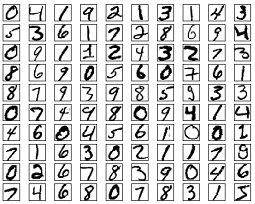
\includegraphics{mnist_100_digits.png}
\caption{The so-called MNIST training sample}
\end{figure}

Simple intuitions about how we recognize shapes - ``a 9 has a loop at
the top, and a vertical stroke in the bottom right'' - turn out to be
not so simple to express algorithmically. When you try to make such
rules precise, you quickly get lost in a morass of exceptions and
caveats and special cases. It seems hopeless.

Neural networks approach the problem in a different way. The idea is to
take a large number of handwritten digits and then develop a system
which can learn from those training examples. By increasing the number
of training examples, the network can learn more about handwriting, and
so improve its accuracy. So while I've shown just 100 training digits
above, perhaps we could build a better handwriting recognizer by using
thousands or even millions or billions of training examples
(\textbf{remember that neural nets are not capable of extrapolating
results !!!}).

Let's try to implement an ANN that is capable of recognize handwritten
digits. To start we need to install two new modules (from the command
line type the following):

\texttt{pip\ install\ keras,\ mnist,\ tensorflow}

Our program will be based on a Convolutional Neural Network (CNN, will
see later other two types of NN) which is designed for image/pattern
recognition. It works essentially by applying on top of an image a
series of filters (matrices) that works as edge detectors and with them
it classifies images according to their features.

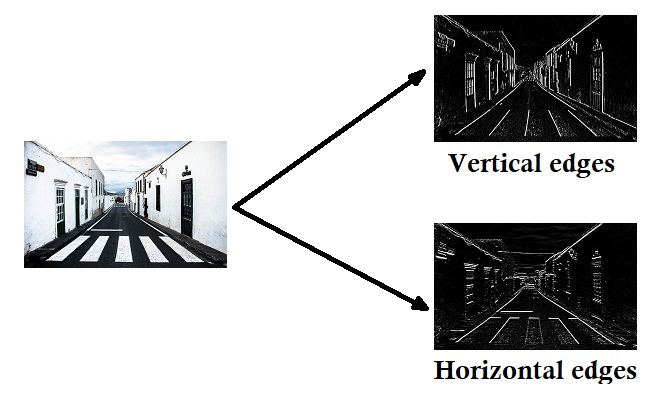
\includegraphics[width=0.8\textwidth]{edges.jpg}

    \begin{Verbatim}[commandchars=\\\{\}]
{\color{incolor}In [{\color{incolor}2}]:} \PY{k+kn}{import} \PY{n+nn}{numpy} \PY{k}{as} \PY{n+nn}{np}
        \PY{c+c1}{\PYZsh{} contains our dataset for training}
        \PY{k+kn}{import} \PY{n+nn}{mnist} 
        \PY{c+c1}{\PYZsh{} keras gives us all the tools to work with NN}
        \PY{k+kn}{from} \PY{n+nn}{keras}\PY{n+nn}{.}\PY{n+nn}{models} \PY{k}{import} \PY{n}{Sequential} 
        \PY{k+kn}{from} \PY{n+nn}{keras}\PY{n+nn}{.}\PY{n+nn}{layers} \PY{k}{import} \PY{n}{Conv2D}\PY{p}{,} \PY{n}{MaxPooling2D}\PY{p}{,} \PY{n}{Dense}\PY{p}{,} \PY{n}{Flatten}
        \PY{k+kn}{from} \PY{n+nn}{keras}\PY{n+nn}{.}\PY{n+nn}{utils} \PY{k}{import} \PY{n}{to\PYZus{}categorical}
        
        \PY{c+c1}{\PYZsh{} load the training and testing set}
        \PY{n}{train\PYZus{}images} \PY{o}{=} \PY{n}{mnist}\PY{o}{.}\PY{n}{train\PYZus{}images}\PY{p}{(}\PY{p}{)} \PY{c+c1}{\PYZsh{} the actual images}
        \PY{n}{train\PYZus{}labels} \PY{o}{=} \PY{n}{mnist}\PY{o}{.}\PY{n}{train\PYZus{}labels}\PY{p}{(}\PY{p}{)} \PY{c+c1}{\PYZsh{} the truth (it is 0, 1, 2...)}
        \PY{n}{test\PYZus{}images} \PY{o}{=} \PY{n}{mnist}\PY{o}{.}\PY{n}{test\PYZus{}images}\PY{p}{(}\PY{p}{)}
        \PY{n}{test\PYZus{}labels} \PY{o}{=} \PY{n}{mnist}\PY{o}{.}\PY{n}{test\PYZus{}labels}\PY{p}{(}\PY{p}{)}
        
        \PY{c+c1}{\PYZsh{} transform data for convenience}
        \PY{n}{train\PYZus{}images} \PY{o}{=} \PY{p}{(}\PY{n}{train\PYZus{}images} \PY{o}{/} \PY{l+m+mi}{255}\PY{p}{)} \PY{o}{\PYZhy{}} \PY{l+m+mf}{0.5}
        \PY{n}{test\PYZus{}images} \PY{o}{=} \PY{p}{(}\PY{n}{test\PYZus{}images} \PY{o}{/} \PY{l+m+mi}{255}\PY{p}{)} \PY{o}{\PYZhy{}} \PY{l+m+mf}{0.5}
        \PY{n}{train\PYZus{}images} \PY{o}{=} \PY{n}{np}\PY{o}{.}\PY{n}{expand\PYZus{}dims}\PY{p}{(}\PY{n}{train\PYZus{}images}\PY{p}{,} \PY{n}{axis}\PY{o}{=}\PY{l+m+mi}{3}\PY{p}{)}
        \PY{n}{test\PYZus{}images} \PY{o}{=} \PY{n}{np}\PY{o}{.}\PY{n}{expand\PYZus{}dims}\PY{p}{(}\PY{n}{test\PYZus{}images}\PY{p}{,} \PY{n}{axis}\PY{o}{=}\PY{l+m+mi}{3}\PY{p}{)}
        
        \PY{c+c1}{\PYZsh{} definition of the actual network}
        \PY{n}{num\PYZus{}filters} \PY{o}{=} \PY{l+m+mi}{8}
        \PY{n}{filter\PYZus{}size} \PY{o}{=} \PY{l+m+mi}{3}
        \PY{n}{pool\PYZus{}size} \PY{o}{=} \PY{l+m+mi}{2}
        
        \PY{c+c1}{\PYZsh{} the input size reflects the size of the image with}
        \PY{c+c1}{\PYZsh{} the numbers 28x28 pixels}
        \PY{c+c1}{\PYZsh{} the output is given by 10 neurons returning the }
        \PY{c+c1}{\PYZsh{} probability that image is in each class.}
        \PY{n}{model} \PY{o}{=} \PY{n}{Sequential}\PY{p}{(}\PY{p}{[}
            \PY{n}{Conv2D}\PY{p}{(}\PY{n}{num\PYZus{}filters}\PY{p}{,} \PY{n}{filter\PYZus{}size}\PY{p}{,} \PY{n}{input\PYZus{}shape}\PY{o}{=}\PY{p}{(}\PY{l+m+mi}{28}\PY{p}{,} \PY{l+m+mi}{28}\PY{p}{,} \PY{l+m+mi}{1}\PY{p}{)}\PY{p}{)}\PY{p}{,} 
            \PY{n}{MaxPooling2D}\PY{p}{(}\PY{n}{pool\PYZus{}size}\PY{o}{=}\PY{n}{pool\PYZus{}size}\PY{p}{)}\PY{p}{,}
            \PY{n}{Flatten}\PY{p}{(}\PY{p}{)}\PY{p}{,}
            \PY{n}{Dense}\PY{p}{(}\PY{l+m+mi}{10}\PY{p}{,} \PY{n}{activation}\PY{o}{=}\PY{l+s+s2}{\PYZdq{}}\PY{l+s+s2}{softmax}\PY{l+s+s2}{\PYZdq{}}\PY{p}{)}
        \PY{p}{]}\PY{p}{)}
        
        \PY{n}{model}\PY{o}{.}\PY{n}{compile}\PY{p}{(}\PY{l+s+s1}{\PYZsq{}}\PY{l+s+s1}{adam}\PY{l+s+s1}{\PYZsq{}}\PY{p}{,} \PY{n}{loss}\PY{o}{=}\PY{l+s+s2}{\PYZdq{}}\PY{l+s+s2}{categorical\PYZus{}crossentropy}\PY{l+s+s2}{\PYZdq{}}\PY{p}{,}
                      \PY{n}{metrics}\PY{o}{=}\PY{p}{[}\PY{l+s+s1}{\PYZsq{}}\PY{l+s+s1}{accuracy}\PY{l+s+s1}{\PYZsq{}}\PY{p}{]}\PY{p}{)}
        
        \PY{n}{model}\PY{o}{.}\PY{n}{fit}\PY{p}{(}\PY{n}{train\PYZus{}images}\PY{p}{,}
                  \PY{n}{to\PYZus{}categorical}\PY{p}{(}\PY{n}{train\PYZus{}labels}\PY{p}{)}\PY{p}{,}
                  \PY{n}{epochs}\PY{o}{=}\PY{l+m+mi}{3}\PY{p}{,}
                  \PY{n}{validation\PYZus{}data}\PY{o}{=}\PY{p}{(}\PY{n}{test\PYZus{}images}\PY{p}{,} \PY{n}{to\PYZus{}categorical}\PY{p}{(}\PY{n}{test\PYZus{}labels}\PY{p}{)}\PY{p}{)}\PY{p}{)}
\end{Verbatim}

    \begin{Verbatim}[commandchars=\\\{\}]
Using TensorFlow backend.

    \end{Verbatim}

    \begin{Verbatim}[commandchars=\\\{\}]
Train on 60000 samples, validate on 10000 samples
Epoch 1/3
60000/60000 [==============================] - 13s 222us/step - loss: 0.3369 - acc: 0.9025 - val\_loss: 0.1855 - val\_acc: 0.9461
Epoch 2/3
60000/60000 [==============================] - 14s 228us/step - loss: 0.1633 - acc: 0.9531 - val\_loss: 0.1273 - val\_acc: 0.9630
Epoch 3/3
60000/60000 [==============================] - 14s 226us/step - loss: 0.1211 - acc: 0.9649 - val\_loss: 0.1092 - val\_acc: 0.9682

    \end{Verbatim}

\begin{Verbatim}[commandchars=\\\{\}]
{\color{outcolor}Out[{\color{outcolor}2}]:} <keras.callbacks.History at 0x7f3bd6db5390>
\end{Verbatim}
            
    \begin{Verbatim}[commandchars=\\\{\}]
{\color{incolor}In [{\color{incolor}10}]:} \PY{n}{predictions} \PY{o}{=} \PY{n}{model}\PY{o}{.}\PY{n}{predict}\PY{p}{(}\PY{n}{test\PYZus{}images}\PY{p}{[}\PY{l+m+mi}{0}\PY{p}{:}\PY{l+m+mi}{2}\PY{p}{]}\PY{p}{)}
         \PY{k}{for} \PY{n}{p} \PY{o+ow}{in} \PY{n}{predictions}\PY{p}{:}
             \PY{n+nb}{print} \PY{p}{(}\PY{p}{[}\PY{l+s+s2}{\PYZdq{}}\PY{l+s+si}{\PYZob{}:.2f\PYZcb{}}\PY{l+s+s2}{\PYZdq{}}\PY{o}{.}\PY{n}{format}\PY{p}{(}\PY{n}{i}\PY{p}{)} \PY{k}{for} \PY{n}{i} \PY{o+ow}{in} \PY{n}{p}\PY{p}{]}\PY{p}{)}
         
         \PY{k}{for} \PY{n}{i} \PY{o+ow}{in} \PY{n+nb}{range}\PY{p}{(}\PY{l+m+mi}{2}\PY{p}{)}\PY{p}{:}
             \PY{n+nb}{print}\PY{p}{(}\PY{l+s+s2}{\PYZdq{}}\PY{l+s+s2}{The CNN predicted }\PY{l+s+si}{\PYZob{}\PYZcb{}}\PY{l+s+s2}{ and it was }\PY{l+s+si}{\PYZob{}\PYZcb{}}\PY{l+s+s2}{\PYZdq{}}\PY{o}{.}\PY{n}{format}\PY{p}{(} \PYZbs{}
                   \PY{n}{np}\PY{o}{.}\PY{n}{argmax}\PY{p}{(}\PY{n}{predictions}\PY{p}{[}\PY{n}{i}\PY{p}{]}\PY{p}{,} \PY{n}{axis}\PY{o}{=}\PY{l+m+mi}{0}\PY{p}{)}\PY{p}{,} \PY{n}{test\PYZus{}labels}\PY{p}{[}\PY{n}{i}\PY{p}{]}\PY{p}{)}\PY{p}{)}
\end{Verbatim}

    \begin{Verbatim}[commandchars=\\\{\}]
['0.00', '0.00', '0.00', '0.00', '0.00', '0.00', '0.00', '1.00', '0.00', '0.00']
['0.00', '0.00', '0.99', '0.00', '0.00', '0.00', '0.01', '0.00', '0.00', '0.00']
The CNN predicted 7 and it was 7
The CNN predicted 2 and it was 2

    \end{Verbatim}

    I have tested the NN using digits written by me:
    
    \begin{center}
      
\includegraphics[width=0.3\textwidth]{due.png}
      
\includegraphics[width=0.3\textwidth]{tre.png}
      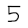
\includegraphics[width=0.3\textwidth]{cinque.png}
    \end{center}
    
and the ANN worked with the three of them. This is the result with my 5:

\begin{Shaded}
\begin{Highlighting}[]
\NormalTok{[}\DecValTok{5}\NormalTok{]}
\NormalTok{[}\FloatTok{0.00}\NormalTok{, }\FloatTok{0.00}\NormalTok{, }\FloatTok{0.00}\NormalTok{, }\FloatTok{0.10}\NormalTok{, }\FloatTok{0.00}\NormalTok{, }\FloatTok{0.89}\NormalTok{, }\FloatTok{0.00}\NormalTok{, }\FloatTok{0.00}\NormalTok{, }\FloatTok{0.00}\NormalTok{, }\FloatTok{0.00}\NormalTok{]}
\end{Highlighting}
\end{Shaded}

Smaller probability \emph{only} 89.4\% (confused by the 3 10\%) \textbf{but
still it works}.

\hypertarget{black-scholes-call-options}{%
\subsection{Black-Scholes call
options}\label{black-scholes-call-options}}

The first practical application concerns the pricing of european call
options. In this case I have generated by myself a large number of call
options with different strikes, maturity, underlying development and
trained the NN using as inputs: volatility, strike, maturity and
underlying price. The truth is the price of the call computed using the
Black-Scholes formula.


\includegraphics[width=0.7\textwidth]{underlyings.png}

In this case I have used a \emph{traditional} NN with an input layer
with 5 neurons (the number of inputs), an hidden layer with 8 neurons
and an output layer with 1 single neuron (since I need just a number,
the price of the call).

    \begin{Verbatim}[commandchars=\\\{\}]
{\color{incolor}In [{\color{incolor} }]:} \PY{c+c1}{\PYZsh{} Regression Example }
        \PY{k+kn}{from} \PY{n+nn}{keras}\PY{n+nn}{.}\PY{n+nn}{models} \PY{k}{import} \PY{n}{Sequential}\PY{p}{,} \PY{n}{load\PYZus{}model}
        \PY{k+kn}{from} \PY{n+nn}{keras}\PY{n+nn}{.}\PY{n+nn}{layers} \PY{k}{import} \PY{n}{Dense}
        \PY{k+kn}{from} \PY{n+nn}{keras}\PY{n+nn}{.}\PY{n+nn}{optimizers} \PY{k}{import} \PY{n}{SGD}
        \PY{k+kn}{from} \PY{n+nn}{keras}\PY{n+nn}{.}\PY{n+nn}{wrappers}\PY{n+nn}{.}\PY{n+nn}{scikit\PYZus{}learn} \PY{k}{import} \PY{n}{KerasRegressor}
        \PY{k+kn}{from} \PY{n+nn}{sklearn}\PY{n+nn}{.}\PY{n+nn}{model\PYZus{}selection} \PY{k}{import} \PY{n}{cross\PYZus{}val\PYZus{}score}
        \PY{k+kn}{from} \PY{n+nn}{sklearn}\PY{n+nn}{.}\PY{n+nn}{model\PYZus{}selection} \PY{k}{import} \PY{n}{train\PYZus{}test\PYZus{}split}
        \PY{k+kn}{from} \PY{n+nn}{sklearn}\PY{n+nn}{.}\PY{n+nn}{metrics} \PY{k}{import} \PY{n}{accuracy\PYZus{}score}
        \PY{k+kn}{import} \PY{n+nn}{pandas} \PY{k}{as} \PY{n+nn}{pd}
        \PY{k+kn}{import} \PY{n+nn}{matplotlib}\PY{n+nn}{.}\PY{n+nn}{pyplot} \PY{k}{as} \PY{n+nn}{plt}
        
        \PY{c+c1}{\PYZsh{}\PYZsh{} just a way to load the dataset}
        \PY{n}{dataset} \PY{o}{=} \PY{n}{pd}\PY{o}{.}\PY{n}{read\PYZus{}csv}\PY{p}{(}\PY{l+s+s2}{\PYZdq{}}\PY{l+s+s2}{training.csv}\PY{l+s+s2}{\PYZdq{}}\PY{p}{)}
        \PY{n}{X\PYZus{}train} \PY{o}{=} \PY{n}{dataset}\PY{o}{.}\PY{n}{iloc}\PY{p}{[}\PY{p}{:}\PY{p}{,} \PY{p}{:}\PY{l+m+mi}{5}\PY{p}{]}\PY{o}{.}\PY{n}{values}
        \PY{n}{Y\PYZus{}train} \PY{o}{=} \PY{n}{dataset}\PY{o}{.}\PY{n}{iloc}\PY{p}{[}\PY{p}{:}\PY{p}{,} \PY{l+m+mi}{5}\PY{p}{]}\PY{o}{.}\PY{n}{values}
        
        \PY{c+c1}{\PYZsh{} NN defintion}
        \PY{n}{model} \PY{o}{=} \PY{n}{Sequential}\PY{p}{(}\PY{p}{)}
        \PY{n}{model}\PY{o}{.}\PY{n}{add}\PY{p}{(}\PY{n}{Dense}\PY{p}{(}\PY{l+m+mi}{8}\PY{p}{,} \PY{n}{input\PYZus{}dim}\PY{o}{=}\PY{l+m+mi}{5}\PY{p}{,} 
                        \PY{n}{kernel\PYZus{}initializer}\PY{o}{=}\PY{l+s+s1}{\PYZsq{}}\PY{l+s+s1}{normal}\PY{l+s+s1}{\PYZsq{}}\PY{p}{,} 
                        \PY{n}{activation}\PY{o}{=}\PY{l+s+s1}{\PYZsq{}}\PY{l+s+s1}{relu}\PY{l+s+s1}{\PYZsq{}}\PY{p}{)}\PY{p}{)}
        \PY{n}{model}\PY{o}{.}\PY{n}{add}\PY{p}{(}\PY{n}{Dense}\PY{p}{(}\PY{l+m+mi}{11}\PY{p}{,} \PY{n}{kernel\PYZus{}initializer}\PY{o}{=}\PY{l+s+s1}{\PYZsq{}}\PY{l+s+s1}{normal}\PY{l+s+s1}{\PYZsq{}}\PY{p}{,} 
                        \PY{n}{activation}\PY{o}{=}\PY{l+s+s1}{\PYZsq{}}\PY{l+s+s1}{relu}\PY{l+s+s1}{\PYZsq{}}\PY{p}{)}\PY{p}{)}
        \PY{n}{model}\PY{o}{.}\PY{n}{add}\PY{p}{(}\PY{n}{Dense}\PY{p}{(}\PY{l+m+mi}{1}\PY{p}{,} \PY{n}{kernel\PYZus{}initializer}\PY{o}{=}\PY{l+s+s1}{\PYZsq{}}\PY{l+s+s1}{normal}\PY{l+s+s1}{\PYZsq{}}\PY{p}{)}\PY{p}{)}
        
        \PY{c+c1}{\PYZsh{} Compile model}
        \PY{n}{model}\PY{o}{.}\PY{n}{compile}\PY{p}{(}\PY{n}{loss}\PY{o}{=}\PY{l+s+s1}{\PYZsq{}}\PY{l+s+s1}{mean\PYZus{}absolute\PYZus{}error}\PY{l+s+s1}{\PYZsq{}}\PY{p}{,} 
                      \PY{n}{optimizer}\PY{o}{=}\PY{l+s+s1}{\PYZsq{}}\PY{l+s+s1}{adam}\PY{l+s+s1}{\PYZsq{}}\PY{p}{,} 
                      \PY{n}{metrics}\PY{o}{=}\PY{p}{[}\PY{l+s+s1}{\PYZsq{}}\PY{l+s+s1}{mse}\PY{l+s+s1}{\PYZsq{}}\PY{p}{]}\PY{p}{)}
        
        \PY{c+c1}{\PYZsh{} perform the actual training}
        \PY{n}{history} \PY{o}{=} \PY{n}{model}\PY{o}{.}\PY{n}{fit}\PY{p}{(}\PY{n}{X\PYZus{}train}\PY{p}{,} 
                            \PY{n}{Y\PYZus{}train}\PY{p}{,} 
                            \PY{n}{epochs}\PY{o}{=}\PY{l+m+mi}{100}\PY{p}{,} 
                            \PY{n}{verbose}\PY{o}{=}\PY{l+m+mi}{1}\PY{p}{,} 
                            \PY{n}{batch\PYZus{}size}\PY{o}{=}\PY{l+m+mi}{100}\PY{p}{)}
\end{Verbatim}

    The training of a neural net is stochastic so it should be run multiple
times to asses its performance.

    \begin{Verbatim}[commandchars=\\\{\}]
{\color{incolor}In [{\color{incolor}13}]:} \PY{k+kn}{import} \PY{n+nn}{pandas} \PY{k}{as} \PY{n+nn}{pd}
         \PY{k+kn}{from} \PY{n+nn}{keras}\PY{n+nn}{.}\PY{n+nn}{models} \PY{k}{import} \PY{n}{load\PYZus{}model}
         \PY{k+kn}{import} \PY{n+nn}{matplotlib}\PY{n+nn}{.}\PY{n+nn}{pyplot} \PY{k}{as} \PY{n+nn}{plt}
         
         \PY{n}{model} \PY{o}{=} \PY{n}{load\PYZus{}model}\PY{p}{(}\PY{l+s+s1}{\PYZsq{}}\PY{l+s+s1}{bs\PYZus{}model.h5.very\PYZus{}very\PYZus{}good}\PY{l+s+s1}{\PYZsq{}}\PY{p}{)}
         
         \PY{n}{dataset} \PY{o}{=} \PY{n}{pd}\PY{o}{.}\PY{n}{read\PYZus{}csv}\PY{p}{(}\PY{l+s+s2}{\PYZdq{}}\PY{l+s+s2}{testing.csv}\PY{l+s+s2}{\PYZdq{}}\PY{p}{)}
         \PY{n}{X\PYZus{}test} \PY{o}{=} \PY{n}{dataset}\PY{o}{.}\PY{n}{iloc}\PY{p}{[}\PY{p}{:}\PY{p}{,} \PY{p}{:}\PY{l+m+mi}{5}\PY{p}{]}\PY{o}{.}\PY{n}{values}
         \PY{n}{Y\PYZus{}test} \PY{o}{=} \PY{n}{dataset}\PY{o}{.}\PY{n}{iloc}\PY{p}{[}\PY{p}{:}\PY{p}{,} \PY{l+m+mi}{5}\PY{p}{]}\PY{o}{.}\PY{n}{values}
         
         \PY{n}{plt}\PY{o}{.}\PY{n}{plot}\PY{p}{(}\PY{n}{model}\PY{o}{.}\PY{n}{predict}\PY{p}{(}\PY{n}{X\PYZus{}test}\PY{p}{[}\PY{l+m+mi}{0}\PY{p}{:}\PY{l+m+mi}{200}\PY{p}{]}\PY{p}{)}\PY{p}{)}
         \PY{n}{plt}\PY{o}{.}\PY{n}{plot}\PY{p}{(}\PY{n}{Y\PYZus{}test}\PY{p}{[}\PY{l+m+mi}{0}\PY{p}{:}\PY{l+m+mi}{200}\PY{p}{]}\PY{p}{)}
         \PY{n}{plt}\PY{o}{.}\PY{n}{show}\PY{p}{(}\PY{p}{)}
\end{Verbatim}

    \begin{center}
    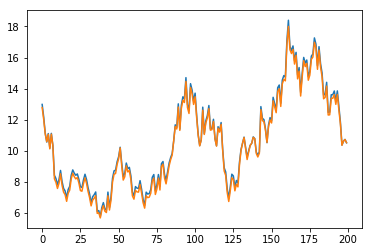
\includegraphics[width=0.7\textwidth]{lecture_10_6_0.png}
    \end{center}
    { \hspace*{\fill} \\}
    
    \hypertarget{technical-analysis}{%
\subsection{Technical Analysis}\label{technical-analysis}}

In finance, technical analysis is a security analysis discipline for
forecasting the direction of prices through the study of past market
data, primarily price and volume. Essentially the analyst looks for
particular patterns in the price time series that are \emph{known} to
develop in predictable ways to take profit of it.

\begin{center}
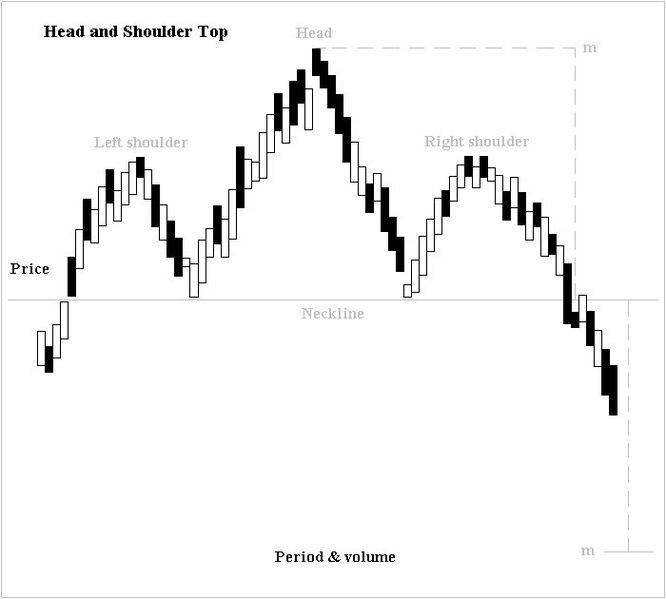
\includegraphics[width=0.6\textwidth]{H_and_s_top_new.jpg}
\includegraphics[width=0.6\textwidth]{Triangle-ascending.jpg}
\includegraphics[width=0.6\textwidth]{image_1.png}
\includegraphics[width=0.6\textwidth]{image_2.png}
\includegraphics[width=0.6\textwidth]{image_0.png}
\end{center}

As you may imagine we will try to develop a CNN (like in the handwriting
case) capable of classifying features in time series to be used in a
technical analysis (this is much faster than having somebody looking at
thousands of time series by eye\ldots{}).

As in the previous application I have generated by myself the training
set simulating 9000 time series (1/3 with head and shoulder patter, 1/3
with triangle pattern and 1/3 with no pattern). To make the training
easier the features have been exagerated.

No pattern

Head and shoulder pattern

Tringle pattern

    \begin{Verbatim}[commandchars=\\\{\}]
{\color{incolor}In [{\color{incolor}17}]:} \PY{k+kn}{import} \PY{n+nn}{numpy} \PY{k}{as} \PY{n+nn}{np}
         \PY{k+kn}{import} \PY{n+nn}{json}
         \PY{k+kn}{from} \PY{n+nn}{keras}\PY{n+nn}{.}\PY{n+nn}{models} \PY{k}{import} \PY{n}{Sequential}\PY{p}{,} \PY{n}{load\PYZus{}model}
         \PY{k+kn}{from} \PY{n+nn}{keras}\PY{n+nn}{.}\PY{n+nn}{layers} \PY{k}{import} \PY{n}{Dense}\PY{p}{,} \PY{n}{Conv1D}\PY{p}{,} \PY{n}{Dropout}
         \PY{k+kn}{from} \PY{n+nn}{keras}\PY{n+nn}{.}\PY{n+nn}{layers} \PY{k}{import} \PY{n}{MaxPooling1D}\PY{p}{,} \PY{n}{GlobalAveragePooling1D}
         \PY{k+kn}{from} \PY{n+nn}{keras}\PY{n+nn}{.}\PY{n+nn}{utils} \PY{k}{import} \PY{n}{to\PYZus{}categorical}
         
         \PY{c+c1}{\PYZsh{} load the training set}
         \PY{k}{with} \PY{n+nb}{open}\PY{p}{(}\PY{l+s+s2}{\PYZdq{}}\PY{l+s+s2}{training\PYZus{}tech\PYZus{}ana\PYZus{}labels.json}\PY{l+s+s2}{\PYZdq{}}\PY{p}{,} \PY{l+s+s2}{\PYZdq{}}\PY{l+s+s2}{r}\PY{l+s+s2}{\PYZdq{}}\PY{p}{)} \PY{k}{as} \PY{n}{f}\PY{p}{:}
             \PY{n}{train\PYZus{}labels} \PY{o}{=} \PY{n}{json}\PY{o}{.}\PY{n}{load}\PY{p}{(}\PY{n}{f}\PY{p}{)}
         
         \PY{n}{train\PYZus{}labels} \PY{o}{=} \PY{n}{train\PYZus{}labels}\PY{p}{[}\PY{p}{:}\PY{l+m+mi}{900}\PY{p}{]}
         \PY{n}{train\PYZus{}images} \PY{o}{=} \PY{p}{[}\PY{p}{]}
         
         \PY{k}{with} \PY{n+nb}{open}\PY{p}{(}\PY{l+s+s2}{\PYZdq{}}\PY{l+s+s2}{training\PYZus{}tech\PYZus{}ana\PYZus{}images.json}\PY{l+s+s2}{\PYZdq{}}\PY{p}{,} \PY{l+s+s2}{\PYZdq{}}\PY{l+s+s2}{r}\PY{l+s+s2}{\PYZdq{}}\PY{p}{)} \PY{k}{as} \PY{n}{f}\PY{p}{:}
             \PY{n}{train\PYZus{}images} \PY{o}{=} \PY{n}{json}\PY{o}{.}\PY{n}{load}\PY{p}{(}\PY{n}{f}\PY{p}{)}
         \PY{n}{train\PYZus{}images} \PY{o}{=} \PY{n}{train\PYZus{}images}\PY{p}{[}\PY{p}{:}\PY{l+m+mi}{900}\PY{p}{]}
         
         \PY{n}{train\PYZus{}images} \PY{o}{=} \PY{n}{np}\PY{o}{.}\PY{n}{array}\PY{p}{(}\PY{n}{train\PYZus{}images}\PY{p}{)}
         \PY{n}{train\PYZus{}images} \PY{o}{=} \PY{n}{np}\PY{o}{.}\PY{n}{expand\PYZus{}dims}\PY{p}{(}\PY{n}{train\PYZus{}images}\PY{p}{,} \PY{n}{axis}\PY{o}{=}\PY{l+m+mi}{3}\PY{p}{)}
         
         \PY{c+c1}{\PYZsh{} define the CNN }
         \PY{n}{model} \PY{o}{=} \PY{n}{Sequential}\PY{p}{(}\PY{p}{)}
         \PY{n}{model}\PY{o}{.}\PY{n}{add}\PY{p}{(}\PY{n}{Conv1D}\PY{p}{(}\PY{n}{filters}\PY{o}{=}\PY{l+m+mi}{80}\PY{p}{,} \PY{n}{kernel\PYZus{}size}\PY{o}{=}\PY{l+m+mi}{20}\PY{p}{,} 
                          \PY{n}{activation}\PY{o}{=}\PY{l+s+s1}{\PYZsq{}}\PY{l+s+s1}{relu}\PY{l+s+s1}{\PYZsq{}}\PY{p}{,} \PY{n}{input\PYZus{}shape}\PY{o}{=}\PY{p}{(}\PY{l+m+mi}{101}\PY{p}{,} \PY{l+m+mi}{1}\PY{p}{)}\PY{p}{)}\PY{p}{)}
         \PY{n}{model}\PY{o}{.}\PY{n}{add}\PY{p}{(}\PY{n}{Conv1D}\PY{p}{(}\PY{n}{filters}\PY{o}{=}\PY{l+m+mi}{80}\PY{p}{,} \PY{n}{kernel\PYZus{}size}\PY{o}{=}\PY{l+m+mi}{15}\PY{p}{,} 
                          \PY{n}{activation}\PY{o}{=}\PY{l+s+s1}{\PYZsq{}}\PY{l+s+s1}{relu}\PY{l+s+s1}{\PYZsq{}}\PY{p}{)}\PY{p}{)}
         \PY{n}{model}\PY{o}{.}\PY{n}{add}\PY{p}{(}\PY{n}{MaxPooling1D}\PY{p}{(}\PY{l+m+mi}{3}\PY{p}{)}\PY{p}{)}
         \PY{n}{model}\PY{o}{.}\PY{n}{add}\PY{p}{(}\PY{n}{Conv1D}\PY{p}{(}\PY{n}{filters}\PY{o}{=}\PY{l+m+mi}{100}\PY{p}{,} \PY{n}{kernel\PYZus{}size}\PY{o}{=}\PY{l+m+mi}{10}\PY{p}{,} 
                          \PY{n}{activation}\PY{o}{=}\PY{l+s+s1}{\PYZsq{}}\PY{l+s+s1}{relu}\PY{l+s+s1}{\PYZsq{}}\PY{p}{)}\PY{p}{)}
         \PY{n}{model}\PY{o}{.}\PY{n}{add}\PY{p}{(}\PY{n}{Conv1D}\PY{p}{(}\PY{n}{filters}\PY{o}{=}\PY{l+m+mi}{100}\PY{p}{,} \PY{n}{kernel\PYZus{}size}\PY{o}{=}\PY{l+m+mi}{5}\PY{p}{,} 
                          \PY{n}{activation}\PY{o}{=}\PY{l+s+s1}{\PYZsq{}}\PY{l+s+s1}{relu}\PY{l+s+s1}{\PYZsq{}}\PY{p}{)}\PY{p}{)}
         \PY{n}{model}\PY{o}{.}\PY{n}{add}\PY{p}{(}\PY{n}{GlobalAveragePooling1D}\PY{p}{(}\PY{p}{)}\PY{p}{)}
         \PY{n}{model}\PY{o}{.}\PY{n}{add}\PY{p}{(}\PY{n}{Dropout}\PY{p}{(}\PY{l+m+mf}{0.5}\PY{p}{)}\PY{p}{)}
         \PY{n}{model}\PY{o}{.}\PY{n}{add}\PY{p}{(}\PY{n}{Dense}\PY{p}{(}\PY{l+m+mi}{3}\PY{p}{,} \PY{n}{activation}\PY{o}{=}\PY{l+s+s2}{\PYZdq{}}\PY{l+s+s2}{softmax}\PY{l+s+s2}{\PYZdq{}}\PY{p}{)}\PY{p}{)}
         \PY{n}{model}\PY{o}{.}\PY{n}{compile}\PY{p}{(}\PY{n}{loss}\PY{o}{=}\PY{l+s+s1}{\PYZsq{}}\PY{l+s+s1}{categorical\PYZus{}crossentropy}\PY{l+s+s1}{\PYZsq{}}\PY{p}{,} 
                       \PY{n}{optimizer}\PY{o}{=}\PY{l+s+s1}{\PYZsq{}}\PY{l+s+s1}{adam}\PY{l+s+s1}{\PYZsq{}}\PY{p}{,} \PY{n}{metrics}\PY{o}{=}\PY{p}{[}\PY{l+s+s1}{\PYZsq{}}\PY{l+s+s1}{accuracy}\PY{l+s+s1}{\PYZsq{}}\PY{p}{]}\PY{p}{)}
         
         \PY{c+c1}{\PYZsh{} make the training}
         \PY{n}{model}\PY{o}{.}\PY{n}{fit}\PY{p}{(}\PY{n}{train\PYZus{}images}\PY{p}{,} \PY{n}{to\PYZus{}categorical}\PY{p}{(}\PY{n}{train\PYZus{}labels}\PY{p}{)}\PY{p}{,} 
                   \PY{n}{epochs}\PY{o}{=}\PY{l+m+mi}{150}\PY{p}{,} \PY{n}{batch\PYZus{}size}\PY{o}{=}\PY{l+m+mi}{35}\PY{p}{,} \PY{n}{verbose}\PY{o}{=}\PY{l+m+mi}{2}\PY{p}{)}
         
         \PY{n}{model}\PY{o}{.}\PY{n}{save}\PY{p}{(}\PY{l+s+s1}{\PYZsq{}}\PY{l+s+s1}{tech\PYZus{}ana.h5}\PY{l+s+s1}{\PYZsq{}}\PY{p}{)}
\end{Verbatim}

    \begin{Verbatim}[commandchars=\\\{\}]
/usr/lib/python3/dist-packages/ipykernel\_launcher.py:20: DeprecationWarning: Both axis > a.ndim and axis < -a.ndim - 1 are deprecated and will raise an AxisError in the future.

    \end{Verbatim}

    \begin{Verbatim}[commandchars=\\\{\}]
Epoch 1/150
 - 1s - loss: 2.0686 - acc: 0.3522
 ...
Epoch 46/150
 - 1s - loss: 0.4162 - acc: 0.7789
...
Epoch 150/150
 - 1s - loss: 0.1258 - acc: 0.9444
    \end{Verbatim}

    To test the perfomance I have created a longer time series and passed as
input to the CNN a sliding time window to simulate the evolution of the
price and a feature that is coming. The goal is to check when the neural
net is capable of predicting the incoming pattern.

    \begin{Verbatim}[commandchars=\\\{\}]
{\color{incolor}In [{\color{incolor}12}]:} \PY{k+kn}{import} \PY{n+nn}{numpy} \PY{k}{as} \PY{n+nn}{np}
         \PY{k+kn}{import} \PY{n+nn}{json}
         \PY{k+kn}{from} \PY{n+nn}{keras}\PY{n+nn}{.}\PY{n+nn}{models} \PY{k}{import} \PY{n}{Sequential}\PY{p}{,} \PY{n}{load\PYZus{}model}
         \PY{k+kn}{from} \PY{n+nn}{keras}\PY{n+nn}{.}\PY{n+nn}{layers} \PY{k}{import} \PY{n}{Dense}\PY{p}{,} \PY{n}{Conv1D}\PY{p}{,} \PY{n}{Dropout}\PY{p}{,} \PY{n}{MaxPooling1D}\PY{p}{,} \PY{n}{GlobalAveragePooling1D}
         \PY{k+kn}{from} \PY{n+nn}{keras}\PY{n+nn}{.}\PY{n+nn}{utils} \PY{k}{import} \PY{n}{to\PYZus{}categorical}
         \PY{k+kn}{from} \PY{n+nn}{matplotlib} \PY{k}{import} \PY{n}{pyplot} \PY{k}{as} \PY{n}{plt}
         
         \PY{n}{test\PYZus{}images} \PY{o}{=} \PY{p}{[}\PY{p}{]}
         
         \PY{k}{with} \PY{n+nb}{open}\PY{p}{(}\PY{l+s+s2}{\PYZdq{}}\PY{l+s+s2}{testing\PYZus{}tech\PYZus{}ana\PYZus{}images\PYZus{}frames.json}\PY{l+s+s2}{\PYZdq{}}\PY{p}{,} \PY{l+s+s2}{\PYZdq{}}\PY{l+s+s2}{r}\PY{l+s+s2}{\PYZdq{}}\PY{p}{)} \PY{k}{as} \PY{n}{f}\PY{p}{:}
             \PY{n}{test\PYZus{}images} \PY{o}{=} \PY{n}{json}\PY{o}{.}\PY{n}{load}\PY{p}{(}\PY{n}{f}\PY{p}{)}
         
         \PY{n}{test\PYZus{}images} \PY{o}{=} \PY{n}{np}\PY{o}{.}\PY{n}{array}\PY{p}{(}\PY{n}{test\PYZus{}images}\PY{p}{)}
         \PY{k}{for} \PY{n}{i} \PY{o+ow}{in} \PY{n+nb}{range}\PY{p}{(}\PY{n}{test\PYZus{}images}\PY{o}{.}\PY{n}{shape}\PY{p}{[}\PY{l+m+mi}{0}\PY{p}{]}\PY{p}{)}\PY{p}{:}
             \PY{n}{plt}\PY{o}{.}\PY{n}{plot}\PY{p}{(}\PY{n}{test\PYZus{}images}\PY{p}{[}\PY{n}{i}\PY{p}{,} \PY{p}{:}\PY{p}{]}\PY{p}{)}
             \PY{n}{plt}\PY{o}{.}\PY{n}{show}\PY{p}{(}\PY{p}{)}
         \PY{n}{test\PYZus{}images} \PY{o}{=} \PY{n}{np}\PY{o}{.}\PY{n}{expand\PYZus{}dims}\PY{p}{(}\PY{n}{test\PYZus{}images}\PY{p}{,} \PY{n}{axis}\PY{o}{=}\PY{l+m+mi}{3}\PY{p}{)}
         
         \PY{n}{model} \PY{o}{=} \PY{n}{load\PYZus{}model}\PY{p}{(}\PY{l+s+s1}{\PYZsq{}}\PY{l+s+s1}{tech\PYZus{}ana\PYZus{}10000.h5}\PY{l+s+s1}{\PYZsq{}}\PY{p}{)}
         
         \PY{n}{predictions} \PY{o}{=} \PY{n}{model}\PY{o}{.}\PY{n}{predict}\PY{p}{(}\PY{n}{test\PYZus{}images}\PY{p}{)}
         \PY{k}{for} \PY{n}{i} \PY{o+ow}{in} \PY{n+nb}{range}\PY{p}{(}\PY{n+nb}{len}\PY{p}{(}\PY{n}{predictions}\PY{p}{)}\PY{p}{)}\PY{p}{:}
             \PY{n+nb}{print} \PY{p}{(}\PY{n}{np}\PY{o}{.}\PY{n}{argmax}\PY{p}{(}\PY{n}{predictions}\PY{p}{[}\PY{n}{i}\PY{p}{]}\PY{p}{)}\PY{p}{,} \PY{n+nb}{max}\PY{p}{(}\PY{n}{predictions}\PY{p}{[}\PY{n}{i}\PY{p}{]}\PY{p}{)}\PY{p}{)}
\end{Verbatim}
      
    \adjustimage{max size={0.3\linewidth}}{lecture_10_10_0.png}
    \adjustimage{max size={0.3\linewidth}}{lecture_10_10_1.png}
    \adjustimage{max size={0.3\linewidth}{0.9\paperheight}}{lecture_10_10_2.png}
    { \hspace*{\fill} \\}
    
    \adjustimage{max size={0.3\linewidth}}{lecture_10_10_3.png}
    \adjustimage{max size={0.3\linewidth}}{lecture_10_10_4.png}
    \adjustimage{max size={0.3\linewidth}}{lecture_10_10_5.png}
    { \hspace*{\fill} \\}
    
    \adjustimage{max size={0.3\linewidth}}{lecture_10_10_6.png}
    \adjustimage{max size={0.3\linewidth}}{lecture_10_10_7.png}
    \adjustimage{max size={0.3\linewidth}}{lecture_10_10_8.png}
    { \hspace*{\fill} \\}
    
    \adjustimage{max size={0.3\linewidth}{0.9\paperheight}}{lecture_10_10_9.png}
    { \hspace*{\fill} \\}
    
    \begin{Verbatim}[commandchars=\\\{\}]
0 0.9059956
0 0.9251846
0 0.9130782
0 0.93703276
0 0.96242875
1 0.56031984
1 0.95728
1 0.88402504
1 1.0
1 1.0

    \end{Verbatim}

    So at the 6th sample the CNN start recognizing the \emph{head and
shoulder} pattern in the price evolution.


    % Add a bibliography block to the postdoc
    
    
    
    \end{document}

\clearpage
\chapter{Copulas and Its Applications}

Copulas (or couplae in Latin) are an interesting mathematical tool to represent correlations between probability distributions. They can be used to describe complex dependencies in multivariate risk models, when more basic tools such as multivariate Gaussian distributions are inappropriate. Another commonly used application is sampling from correlated random variables.

In this Chapter the copula concept is reviewed and some example applications are shown. 
Before going into the copulas we need to learn how to transform a distribution into another using the \emph{probability integral transform}. 

\section{Distribution Transformation}\label{distribution-transformation}

Distribution transformation is a very useful tool which will be
extensively used with the copula concept that we discuss in the next
Section. The technique we are going to outline transforms every random
variable, regardless its distribution, into uniform and vice versa and is called
\emph{probability integral transform} or (percentile-to-percentile
transform).

Computationally, this method involves computing the quantile function (see Section~\ref{quantile-function}) of
a distribution, in other words, computing the cumulative
distribution function ($F(x)$) of a distribution (which maps a number
to a probability between 0 and 1) and then inverting that
function. We won't go into the details but we will just show few
examples of how this can be done in \(\tt{python}\).

Imagine we want to transform an uniform distribution into a Gaussian.
The transformation takes uniform samples of a number \(u\) between 0 and
1, interpreted as a probability, and then returns $F^{-1}(u)$. 

Table~\ref{tab:transformation} shows samples taken from the
uniform distribution and their representation on the standard normal
distribution determined using the algorithm explained above.

\begin{table}[h]
  \centering
  \begin{tabular}{|c|c|}
    \hline
    \(\mathbf{u}\) & \(\mathbf{F^{-1}(u)}\) \\
    \hline
    0.5 & 0 \\
    \hline
    .975 & 1.95996 \\
    \hline
    .995 & 2.5758 \\
    \hline
    .999999 & 4.75342 \\
    \hline
    \(1-2^{-52}\) & 8.12589 \\
    \hline
  \end{tabular}
  \caption{Comparison of values of the uniform distribution and the corresponding Gaussian quantiles.}
\label{tab:transformation}
\end{table}

Now let's see how this can be done with \texttt{python}. The first step is to sample
uniformly distributed values between 0 and 1. This can be done either using \texttt{random.random} like in Section~\ref{pseudo-random-numbers} or with \texttt{scipy.stats.uniform}. Each distribution defined in \texttt{scipy.stats} has a convenient method \texttt{rvs(size=aSize)} (random variable sample) to sample from it as many time as specified by the arguments \texttt{size}. Usually the second method is preferred since it exploits \texttt{numpy.array} and let us avoid a lot of for-loop cycles.

In any case in the left plot of Fig.~\ref{fig:uniform_and_gauss} the resulting distribution is shown.

\begin{tcolorbox}[breakable, size=fbox, boxrule=1pt, pad at break*=1mm,colback=cellbackground, colframe=cellborder]
\begin{Verbatim}[commandchars=\\\{\}]
\PY{k+kn}{from} \PY{n+nn}{scipy} \PY{k}{import} \PY{n}{stats}
\PY{n}{x} \PY{o}{=} \PY{n}{stats}\PY{o}{.}\PY{n}{uniform}\PY{p}{(}\PY{l+m+mi}{0}\PY{p}{,} \PY{l+m+mi}{1}\PY{p}{)}\PY{o}{.}\PY{n}{rvs}\PY{p}{(}\PY{l+m+mi}{10000}\PY{p}{)}
\end{Verbatim}
\end{tcolorbox}

Next we want to transform these samples so that instead of uniform they
are normally distributed. As we have seen, see Section~\ref{quantile-function} the transform that does this
is the inverse of the cumulative density function of the normal 
distribution, or \((\tt{ppf(x))}\) in \texttt{oython}. 

In the right plot of Fig.~\ref{fig:uniform_and_gauss} the Gaussian obtained 
with the code below is shown

\begin{figure}[h]
  \centering
  \includegraphics[width=1.\textwidth]{figures/uniform_gauss.png}
  \caption{On the left the generated uniform distribution, on the right its Gaussian transform.}
  \label{fig:uniform_and_gauss}
\end{figure}

\begin{tcolorbox}[breakable, size=fbox, boxrule=1pt, pad at break*=1mm,colback=cellbackground, colframe=cellborder]
\begin{Verbatim}[commandchars=\\\{\}]
\PY{n}{norm} \PY{o}{=} \PY{n}{stats}\PY{o}{.}\PY{n}{norm}\PY{p}{(}\PY{p}{)} 
\PY{n}{x\PYZus{}trans} \PY{o}{=} \PY{n}{norm}\PY{o}{.}\PY{n}{ppf}\PY{p}{(}\PY{n}{x}\PY{p}{)}
\end{Verbatim}
\end{tcolorbox}

If we plot them together in a 2D plot we can get a sense of what is
going on using the inverse CDF transformation.
Indeed it stretches the outer regions of the uniform to yield a
normal distribution. The transformation is shown in Fig.~\ref{fig:uniform_to_gauss}. 
    
\begin{figure}[htbp]
  \centering
  \includegraphics[width=0.5\textwidth]{figures/lesson6_7_0.png}
  \caption{2D plot showing the transformation that maps our initial uniform distribution to the resulting Gaussian.}
  \label{fig:uniform_to_gauss}
\end{figure}
    
The nice thing of this technique is that it can be used
for any arbitrary (uni-variate) probability distribution, like for
example \href{https://en.wikipedia.org/wiki/Student\%27s\_t-distribution}{t-Student}
or \href{https://en.wikipedia.org/wiki/Gumbel_distribution}{Gumbel}.
A similar transformation from uniform to t-Student is shown in Fig.~\ref{fig:uniform_to_tstudent}.

\begin{tcolorbox}[breakable, size=fbox, boxrule=1pt, pad at break*=1mm,colback=cellbackground, colframe=cellborder]
\begin{Verbatim}[commandchars=\\\{\}]
\PY{n}{t} \PY{o}{=} \PY{n}{stats}\PY{o}{.}\PY{n}{t}\PY{p}{(4}\PY{p}{)} 
\PY{n}{x\PYZus{}trans} \PY{o}{=} \PY{n}{t}\PY{o}{.}\PY{n}{ppf}\PY{p}{(}\PY{n}{x}\PY{p}{)}
\end{Verbatim}
\end{tcolorbox}

\begin{figure}[htbp]
  \centering
  \includegraphics[width=0.5\textwidth]{figures/lesson6_9_0.png}
  \caption{2D plot showing the transformation that maps a uniform distribution to a t-Student.}
  \label{fig:uniform_to_tstudent}
\end{figure}

Clearly to do the opposite transformation, from an arbitrary distribution
to the uniform, we can just apply the inverse of the inverse CDF, that is the CDF itself\ldots
In such a way we can go from distribution A to distribution B passing through 
a uniform distribution rather quickly. An example is shown in Figure~\ref{fig:a_to_b_to_a}.

\begin{figure}[htbp]
	\centering
	\includegraphics[width=1.\textwidth]{figures/lesson6_11_0.png}
	\caption{Example of transformation, it starts with a uniform distribution, goes into a Gaussian and back to the initial uniform.}
	\label{fig:a:_to_b_to_a}
\end{figure}

\section{Copula}\label{copula}

In probability theory a \emph{copula} \(C(U_1, U_2, \ldots, U_n, \rho)\)
is a multivariate (multidimensional) cumulative distribution function
for which the marginal probability distributions (i.e. the probability
distribution of each dimension) are uniform on the
interval \([0, 1]\) (\(U_i \approx\)uniform(0,1)).
\(\rho\) represent the correlation between each variable.

Copulas are used to describe the dependencies between random variables and
have been widely used in quantitative finance to model risk. Copulas are popular since
they allow to easily model and estimate the distribution of random
vectors by representing marginals and their correlation separately.

Despite the obscure and daunting definition given above the concept of copula is
quite simple so let's try to clarify it a bit with a practical example.

\subsection{Example Problem Case}\label{example-problem-case}

Imagine to measure two variables that are 
correlated. For example, we look at various rivers and for every river
we look at the maximum water level of that river over a certain
time-period. In addition, we also count how many months each river
caused floods.

For the probability distribution of the maximum level of the river we
know that maximums are Gumbel distributed, while the number of floods
can be modeled according to a
\href{https://en.wikipedia.org/wiki/Beta_distribution}{\emph{Beta}}
distribution.

Clearly it is pretty reasonable to assume that the maximum level and the
number of floods is going to be correlated, however we don't know how
we could model that correlated probability distribution.
Above we only
specified the distributions for individual variables, irrespective of
the other one (i.e. the marginals), in reality we are dealing with a
\emph{joint distribution} of both of these together.

And here is where copulas come to our rescue.

Copulas essentially allow to decompose a joint probability distribution
into their marginals (which by definition have no correlation) and a
function which \textbf{couples} (hence the name) them together and thus allows us
to specify the correlation separately. The copula is just that coupling
function.

\subsection{Adding Correlation with Gaussian Copulas}\label{adding-correlation-with-gaussian-copulas}

How does this help us with our problem of creating a custom joint
probability distribution for maximum water level and floods ?

We are actually almost done already, we saw before how to convert
anything uniformly distributed to an arbitrary probability distribution.
So that means we just need to generate uniformly distributed data with the
correlation we want and then transform the marginals into the desired
distributions (Gumbel and Beta in our example).

How do we do that ?

\begin{itemize}
\tightlist
\item
  simulate a sample from a multivariate distribution with the specific correlation structure;
\item
  transform so that the marginals are uniform;
\item
  finally transform the uniform marginals to whatever we like.
\end{itemize}

In this example we sample from a multivariate (2D) normal with a 0.5 correlation, 
see Fig.~ \ref{fig:multivariate_with_correlation}, although this is not mandatory since
we could model correlations with different distribution either.

\begin{tcolorbox}[breakable, size=fbox, boxrule=1pt, pad at break*=1mm,colback=cellbackground, colframe=cellborder]
\begin{Verbatim}[commandchars=\\\{\}]
\PY{n}{mvnorm} \PY{o}{=} \PY{n}{stats}\PY{o}{.}\PY{n}{multivariate\PYZus{}normal}\PY{p}{(}\PY{n}{mean}\PY{o}{=}\PY{p}{[}\PY{l+m+mi}{0}\PY{p}{,} \PY{l+m+mi}{0}\PY{p}{]} \PY{p}{,} \PY{n}{cov}\PY{o}{=}\PY{p}{[}\PY{p}{[}\PY{l+m+mi}{1}\PY{p}{,} \PY{l+m+mf}{0.5}\PY{p}{]}\PY{p}{,}
                                                      \PY{p}{[}\PY{l+m+mf}{0.5}\PY{p}{,} \PY{l+m+mi}{1}\PY{p}{]}\PY{p}{]}\PY{p}{)}
\PY{n}{x} \PY{o}{=} \PY{n}{mvnorm}\PY{o}{.}\PY{n}{rvs}\PY{p}{(}\PY{l+m+mi}{100000}\PY{p}{)}
\end{Verbatim}
\end{tcolorbox}

\begin{figure}[htb]
  \centering
  \includegraphics[width=0.5\textwidth]{figures/lesson6_14_0.png}
  \caption{2D multivariate normal distribution with a correlation factor of 0.5.}
  \label{fig:multivariate_with_correlation}
\end{figure}
    
Now use what we have just learned to make the marginals uniform using
the \(\tt{cdf}\) function of the normal distribution:

\begin{tcolorbox}[breakable, size=fbox, boxrule=1pt, pad at break*=1mm,colback=cellbackground, colframe=cellborder]
\begin{Verbatim}[commandchars=\\\{\}]
\PY{n}{norm} \PY{o}{=} \PY{n}{stats}\PY{o}{.}\PY{n}{norm}\PY{p}{(}\PY{p}{)}
\PY{n}{x\PYZus{}unif} \PY{o}{=} \PY{n}{norm}\PY{o}{.}\PY{n}{cdf}\PY{p}{(}\PY{n}{x}\PY{p}{)}
\end{Verbatim}
\end{tcolorbox}

The plots shown in Fig.~\ref{fig:copula} are usually how copulas are visualized.

\begin{figure}[p]
\centering
\includegraphics[width=0.45\textwidth]{figures/lesson6_16_0.png}
\quad
\includegraphics[width=0.5\textwidth]{figures/copula_3d.png}
\caption{Graphical representations of the copula, 2D on the left, 3D on the right.}
\label{fig:copula}
\end{figure}

Finally we can just transform the obtained marginals again from uniform to what we want
(i.e. Gumbel and Beta in our river example):

\begin{tcolorbox}[breakable, size=fbox, boxrule=1pt, pad at break*=1mm,colback=cellbackground, colframe=cellborder]
\begin{Verbatim}[commandchars=\\\{\}]
\PY{n}{m1} \PY{o}{=} \PY{n}{stats}\PY{o}{.}\PY{n}{gumbel\PYZus{}l}\PY{p}{(}\PY{p}{)}
\PY{n}{m2} \PY{o}{=} \PY{n}{stats}\PY{o}{.}\PY{n}{beta}\PY{p}{(}\PY{n}{a}\PY{o}{=}\PY{l+m+mi}{10}\PY{p}{,} \PY{n}{b}\PY{o}{=}\PY{l+m+mi}{3}\PY{p}{)}


\end{Verbatim}
\end{tcolorbox}

Left plot of Figure~\ref{fig:gumbel_beta_with_corr} shows the two marginals and the joint distribution.
    
To see that it is actually working as expected we should now compare the joint
distributions with and without correlation. Compare the two plots in Figure~\ref{fig:gumbel_beta_with_corr} to spot the difference.

\begin{tcolorbox}[breakable, size=fbox, boxrule=1pt, pad at break*=1mm,colback=cellbackground, colframe=cellborder]
\begin{Verbatim}[commandchars=\\\{\}]
\PY{c+c1}{\PYZsh{} sample from Gumbel}
\PY{n}{x1} \PY{o}{=} \PY{n}{m1}\PY{o}{.}\PY{n}{rvs}\PY{p}{(}\PY{l+m+mi}{10000}\PY{p}{)}
\PY{c+c1}{\PYZsh{} sample from Beta}
\PY{n}{x2} \PY{o}{=} \PY{n}{m2}\PY{o}{.}\PY{n}{rvs}\PY{p}{(}\PY{l+m+mi}{10000}\PY{p}{)}
\end{Verbatim}
\end{tcolorbox}

\begin{figure}[p]
  \centering
  \includegraphics[width=0.45\textwidth]{figures/lesson6_18_0.png}
  \quad
  \includegraphics[width=0.45\textwidth]{figures/lesson6_20_0.png}
  \caption{Marginalized Gumbel and Beta distributions and their joint with (left) and without (right) correlation.}
  \label{fig:gumbel_beta_with_corr}
\end{figure}
    
Using the uniform distribution as a common base for our transformations
we can easily introduce correlations and flexibly construct complex
probability distributions. 

As a final note, the \emph{Sklar's theorem} states that any multivariate joint distribution
can be written in terms of uni-variate marginal distribution functions
and a copula which describes the dependence structure between the
variables.

Everything discussed in this Section can be easily generalized to higher dimensions.

%\subsection{Other Copulas}
%In the previous Section we have seen an application of a Gaussian copula but exists many other different 
%kind of copulas. Two typical examples are the t-copula and the Clayton copula.

%\subsubsection{t-copula}

%\subsubsection{Clayton copula}

\subsection{Generate Correlated Distributions}\label{generate-correlated-distributions}

If we need to generate numbers from correlated distribution we can
follow similar steps to those described before:

\begin{itemize}
\tightlist
\item
  generate a random vector \(\mathbf{x}=(x_1, x_2,\ldots)\) from the
  original multivariate distribution;
\item
  determine the single \(U_i(x_i)\) by applying \(\tt{cdf}\) to each
  \(x_i\);
\item
  transform again each \(U_i(x_i)\) to the desired marginal
  distributions using \(\tt{ppf}\);
\item
  each component of the vector \(\mathbf{x}\) is now converted to a set
  of random numbers drawn from the desired distributions, with the
  appropriate correlation.
\end{itemize}

A practical application concerns the probability of default. 
Imagine three companies ($A$, $B$ and $C$) which have a
cumulative probability of defaulting within the next two years of 10\%.
Let's try to compute the probabilities to have the three of them all
defaulting within the next two years in two cases: independent default probabilities and perfectly correlated probabilities.

In the first case (independent probabilities), the
odds to get three defaults within two years will be the product
of the single probabilities, hence:

\[\mathbb{P}_{\mathrm{uncorr}} = 10\% \cdot 10\% \cdot 10\% = 0.1 \%\]

We can verify this in \(\tt{python}\) by applying the method outlined above: first generate a random sample from an uncorrelated multivariate normal distribution, then transform each sampled vector into uniform distribution with the \(\tt{norm.cdf}\) function (i.e. we
convert the samples into cumulative probabilities) and then count how many times the
three of them are lower than 10\% to check whether a default occurred in next two year.

\begin{tcolorbox}[breakable, size=fbox, boxrule=1pt, pad at break*=1mm,colback=cellbackground, colframe=cellborder]
\begin{Verbatim}[commandchars=\\\{\}]
\PY{k+kn}{from} \PY{n+nn}{scipy}\PY{n+nn}{.}\PY{n+nn}{stats} \PY{k}{import} \PY{n}{multivariate\PYZus{}normal}\PY{p}{,} \PY{n}{uniform}\PY{p}{,} \PY{n}{norm}
\PY{k+kn}{import} \PY{n+nn}{numpy}
	
\PY{n}{numpy}\PY{o}{.}\PY{n}{random}\PY{o}{.}\PY{n}{seed}\PY{p}{(}\PY{l+m+mi}{10}\PY{p}{)}
\PY{n}{trials} \PY{o}{=}\PY{l+m+mi}{10000}
\PY{n}{mvnorm\PYZus{}no\PYZus{}corr} \PY{o}{=} \PY{n}{multivariate\PYZus{}normal}\PY{p}{(}\PY{n}{mean}\PY{o}{=}\PY{p}{[}\PY{l+m+mi}{0}\PY{p}{,} \PY{l+m+mi}{0}\PY{p}{,} \PY{l+m+mi}{0}\PY{p}{]}\PY{p}{,} \PY{n}{cov}\PY{o}{=}\PY{p}{[}\PY{p}{[}\PY{l+m+mi}{1}\PY{p}{,} \PY{l+m+mi}{0}\PY{p}{,} \PY{l+m+mi}{0}\PY{p}{]}\PY{p}{,}
                                                          \PY{p}{[}\PY{l+m+mi}{0}\PY{p}{,} \PY{l+m+mi}{1}\PY{p}{,} \PY{l+m+mi}{0}\PY{p}{]}\PY{p}{,}
                                                          \PY{p}{[}\PY{l+m+mi}{0}\PY{p}{,} \PY{l+m+mi}{0}\PY{p}{,} \PY{l+m+mi}{1}\PY{p}{]}\PY{p}{]}\PY{p}{)}
\PY{n}{defaults} \PY{o}{=} \PY{l+m+mi}{0}
\PY{n}{x} \PY{o}{=} \PY{n}{mvnorm\PYZus{}no\PYZus{}corr}\PY{o}{.}\PY{n}{rvs}\PY{p}{(}\PY{n}{trials}\PY{p}{)}
\PY{n}{x\PYZus{}trans} \PY{o}{=} \PY{n}{norm}\PY{o}{.}\PY{n}{cdf}\PY{p}{(}\PY{n}{x}\PY{p}{)}
\PY{k}{for} \PY{n}{i} \PY{o+ow}{in} \PY{n+nb}{range}\PY{p}{(}\PY{n+nb}{len}\PY{p}{(}\PY{n}{x\PYZus{}trans}\PY{p}{)}\PY{p}{)}\PY{p}{:}
    \PY{k}{if} \PY{n}{x\PYZus{}trans}\PY{p}{[}\PY{n}{i}\PY{p}{]}\PY{p}{[}\PY{l+m+mi}{0}\PY{p}{]} \PY{o}{\PYZlt{}} \PY{l+m+mf}{0.1} \PY{o+ow}{and} \PY{n}{x\PYZus{}trans}\PY{p}{[}\PY{n}{i}\PY{p}{]}\PY{p}{[}\PY{l+m+mi}{1}\PY{p}{]} \PY{o}{\PYZlt{}} \PY{l+m+mf}{0.1} \PY{o+ow}{and} \PY{n}{x\PYZus{}trans}\PY{p}{[}\PY{n}{i}\PY{p}{]}\PY{p}{[}\PY{l+m+mi}{2}\PY{p}{]} \PY{o}{\PYZlt{}} \PY{l+m+mf}{0.1}\PY{p}{:}
	\PY{n}{defaults} \PY{o}{+}\PY{o}{=} \PY{l+m+mi}{1}
	
\PY{n+nb}{print} \PY{p}{(}\PY{l+s+s2}{\PYZdq{}}\PY{l+s+s2}{Defaults w/o correlation: }\PY{l+s+si}{\PYZob{}:.2f\PYZcb{}}\PY{l+s+s2}{\PYZpc{}}\PY{l+s+s2}{\PYZdq{}}\PY{o}{.}\PY{n}{format}\PY{p}{(}\PY{n}{defaults}\PY{o}{/}\PY{n}{trials}\PY{o}{*}\PY{l+m+mi}{100}\PY{p}{)}\PY{p}{)}

Defaults w/o correlation: 0.10\%
\end{Verbatim}
\end{tcolorbox}
The result is 0.1\% as expected.

If we repeat the same Monte Carlo experiment with perfectly correlated
default probabilities we have

\begin{tcolorbox}[breakable, size=fbox, boxrule=1pt, pad at break*=1mm,colback=cellbackground, colframe=cellborder]
\begin{Verbatim}[commandchars=\\\{\}]
\PY{n}{mvnorm\PYZus{}corr} \PY{o}{=} \PY{n}{multivariate\PYZus{}normal}\PY{p}{(}\PY{n}{mean}\PY{o}{=}\PY{p}{[}\PY{l+m+mi}{0}\PY{p}{,}\PY{l+m+mi}{0}\PY{p}{,}\PY{l+m+mi}{0}\PY{p}{]}\PY{p}{,} \PY{n}{cov}\PY{o}{=}\PY{p}{[}\PY{p}{[}\PY{l+m+mi}{1}\PY{p}{,} \PY{l+m+mf}{0.999999}\PY{p}{,} \PY{l+m+mf}{0.999999}\PY{p}{]}\PY{p}{,}
                                                     \PY{p}{[}\PY{l+m+mf}{0.999999}\PY{p}{,} \PY{l+m+mi}{1}\PY{p}{,} \PY{l+m+mf}{0.999999}\PY{p}{]}\PY{p}{,}
                                                     \PY{p}{[}\PY{l+m+mf}{0.999999}\PY{p}{,} \PY{l+m+mf}{0.999999}\PY{p}{,} \PY{l+m+mi}{1}\PY{p}{]}\PY{p}{]}\PY{p}{)}
\PY{n}{defaults} \PY{o}{=} \PY{l+m+mi}{0}
\PY{n}{x} \PY{o}{=} \PY{n}{mvnorm\PYZus{}corr}\PY{o}{.}\PY{n}{rvs}\PY{p}{(}\PY{n}{trials}\PY{p}{)}
\PY{n}{x\PYZus{}trans} \PY{o}{=} \PY{n}{norm}\PY{o}{.}\PY{n}{cdf}\PY{p}{(}\PY{n}{x}\PY{p}{)}
\PY{k}{for} \PY{n}{i} \PY{o+ow}{in} \PY{n+nb}{range}\PY{p}{(}\PY{n+nb}{len}\PY{p}{(}\PY{n}{x\PYZus{}trans}\PY{p}{)}\PY{p}{)}\PY{p}{:}
    \PY{k}{if} \PY{n}{x\PYZus{}trans}\PY{p}{[}\PY{n}{i}\PY{p}{]}\PY{p}{[}\PY{l+m+mi}{0}\PY{p}{]} \PY{o}{\PYZlt{}} \PY{l+m+mf}{0.1} \PY{o+ow}{and} \PY{n}{x\PYZus{}trans}\PY{p}{[}\PY{n}{i}\PY{p}{]}\PY{p}{[}\PY{l+m+mi}{1}\PY{p}{]} \PY{o}{\PYZlt{}} \PY{l+m+mf}{0.1} \PY{o+ow}{and} \PY{n}{x\PYZus{}trans}\PY{p}{[}\PY{n}{i}\PY{p}{]}\PY{p}{[}\PY{l+m+mi}{2}\PY{p}{]} \PY{o}{\PYZlt{}} \PY{l+m+mf}{0.1}\PY{p}{:}
        \PY{n}{defaults} \PY{o}{+}\PY{o}{=} \PY{l+m+mi}{1}

\PY{n+nb}{print} \PY{p}{(}\PY{l+s+s2}{\PYZdq{}}\PY{l+s+s2}{Defaults w/ correlation: }\PY{l+s+si}{\PYZob{}:.2f\PYZcb{}}\PY{l+s+s2}{\PYZpc{}}\PY{l+s+s2}{\PYZdq{}}\PY{o}{.}\PY{n}{format}\PY{p}{(}\PY{n}{defaults}\PY{o}{/}\PY{n}{trials}\PY{o}{*}\PY{l+m+mi}{100}\PY{p}{)}\PY{p}{)}

Defaults w/ correlation: 9.89\%
\end{Verbatim}
\end{tcolorbox}
In this case the result is close to 10\%, like we had only one single company. 
Indeed given the perfect correlation between the probabilities either there is no default or three
"simultaneous" defaults with 10\% probability.

\clearpage
\chapter{Modeling Correlation between Risks}

In credit derivative valuation and credit risk management, one of the
fundamentally important issues is the estimate of default
probabilities and their correlations. For this, generally speaking,
there are two ways: using historical default data or using mathematical
models.

Historical default data has played an important role in the estimation
of default probabilities. However, because default events are rare,
there is very limited default data available. Moreover, historical data
reflects the historical default pattern only and it may not be a proper
indicator of the future. This makes the estimate of default
probabilities from historical data difficult and inexact. To use this
same data to estimate default correlations is even more difficult and
more inexact.

The market trend now is towards more and more to the use of mathematical
models that don't rely on historical default data. In
Chapter~\ref{credit_default_swaps} we have seen how it is possible to derive default 
probabilities from market data,
here we will see how the copula can be used to model their correlations. 

\section{One Factor Gaussian Copula Model}\label{standard-market-model}
While there are several types of copula function models, the first
introduced was the \emph{one-factor Gaussian copula model}. This model has,
above all, the advantage that can be solved semi-analytically.

Consider a portfolio of \(N\) bonds and assume that the marginal
probabilities of default are known for each issuer. Define:

\begin{itemize}
	\tightlist
	\item
	\(t_i\), the time of default of the \(i^{th}\) company:
	\item
	\(Q_i(t)\), the cumulative probability that company \(i\) will default
	before time \(t\); that is, the probability that \(t_i \le t\).
\end{itemize}

To generate a one-factor model for the \(t_i\) we define random
variables \(X_i\) \((1\le i \le N)\)
\begin{equation}
X_i = a_i M + \sqrt{1-a_i^2}Z_i,\qquad i = 1, 2,\ldots, N
\label{eq:normalized_var}
\end{equation}
where \(M\) and the \(Z_i\) are independent zero-mean unit-variance  distributions (hence $X_i$ are also distributed with zero-mean and unit standard-deviation) and \(-1 \le a_i \lt 1\).

Eq.~\ref{eq:normalized_var} defines a correlation structure between the
\(X_i\) which are dependent on a single common factor \(M\). The $Z_i$ term is usually 
called the idiosyncratic component of default. 
The correlation between \(X_i\) and \(X_j\) is

\[
\mathrm{Corr}(X_i, X_j) = \cfrac{\mathbb{E}[(X_i-\mu_i)(X_j-\mu_j)]}{\sigma_{i}\sigma_{j}} =\mathbb{E}[X_i X_j] = a_i a_j \mathbb{E}[M^2] = a_i a_j
\]
where we just exploit the definition of $X_i$ and its properties.

%Assume that the $i^{th}$ company has defaulted by the time $t_i$ if $X_i$ is below a threshold value $\bar{x}_i(t_i)$.
If $F_i$ is the cumulative distribution function of the $X_i$,
with a percentile to percentile transformation we can map the \(X_i\) to the \(t_i\), so that $Q_i(t_i) = \mathbb{P}(X_i\le x)=F_i(x)$.
Therefore a point \(X_i = x\) is transformed to \(t_i = t\) where
\(x = F_i^{-1}[Q_i(t)]\).

Let's note that, \textbf{conditional} on $M$, the $N$ default events are \textbf{independent}. So we can write
\begin{equation}
\begin{split}
Q_i(t_i|M) = \mathbb{P}(X_i\le x|M) &= \mathbb{P}(a_i M + \sqrt{1-a_i^2}Z_i\le x) =\\
&= \mathbb{P}\left(Z_i\le \cfrac{x-a_i M}{\sqrt{1-a_i^2}}\right)
=H_i\left(\cfrac{F^{-1}[Q(t_i)]-a_i M}{\sqrt{1-a_i^2}}\right)
\end{split}
\label{eq:generic_copula}
\end{equation}
where $H_i$ is the cumulative distribution function of the $Z_i$.

Although in principle any distribution could be used for \(M\) and the
\(Z\)'s (provided they have zero mean and unit variance), one common
choice is to let them be standard normal distributions (resulting in a
Gaussian copula).
So we can rewrite Eq.~\ref{eq:generic_copula} as

\begin{equation}
Q_i(t_i|M) = \Phi\left(\cfrac{\Phi^{-1}[Q(t_i)]-a_i M}{\sqrt{1-a_i^2}}\right)
\label{eq:gaussian_one_factor_copula}
\end{equation}
where $\Phi$ denotes the cumulative distribution function of the standard normal distribution.

If we call $\mathcal{C}(t_1,\ldots,t_N)$ the joint distribution of the default times of the $N$ bonds in the portfolio then

\[
\mathcal{C}(t_1,\ldots,t_N)=\Phi_{A}(\Phi^{-1}(Q_1(t_1)),\ldots,\Phi^{-1}(Q_N(t_N)))
\]
where $A$ is the correlation matrix of the default probabilities, is the one factor Gaussian copula model (one factor because there is only a random variable, $M$, which determines the correlation between $X_i$).

Clearly different choices of distributions result in different copula models, and in different natures of the default dependence. For example, copulas where the \(M\) have heavy tails generate models where there is a
greater likelihood of a clustering of early defaults for several
companies.

\subsection{Standard Market Model}\label{standard-market-model}

Assume the following two assumptions are made:

\begin{itemize}
	\tightlist
	\item
	all the companies have the same default intensity (hazard rates), i.e, \(\lambda_i = \lambda\) (which means they all have the same default probabilities);
	\item
	the pairwise default correlations are the same, i.e \(a_i = a\); in other words the contribution of the market
	component $M$ is the same for all the companies and the correlation between any two companies is constant, \(\rho = a^2\).
\end{itemize}

Under these assumptions, given the market situation \(M = m\), all the
companies have the same cumulative default probability
\(DP_{t|m}=Q_i(t_i|m)=\mathbb{P}(X_i < x|m)\). 
Moreover, for a given value of the
market component \(M\), the defaults are mutually independent for all
the underlying companies. 

Letting \(l_{t|m}\) be the total defaults that
have occurred by time \(t\) conditional on the market condition
\(M = m\), then \(l_{t|m}\) follows a binomial distribution (see Appendix~\ref{appendix1}), and

\[DP(l_{t|m} = j) = \cfrac{N!}{j!(N-j)!}DP^j_{t|m}(1-DP_{t|m})^{N-j},\qquad  j=0, 1, 2,\ldots,N\]

In general to evaluate any function of $DP$, say $g(DP(l_t))$, regardless the parameter $M$ is necessary to average according to the following integral

\begin{equation}
g(DP(l_{t} = j)) = \int_{-\infty}^{\infty}{g(DP(l_{t|m} = j))\cdot f_M(m)dm}
\label{eq:gaussian_quadrature}
\end{equation}

where $f_M(m)$ is the probability density function (PDF) of the random variable $M$.

With the assumption that have been made the one factor model is also called \emph{Market Standard Model}.

If the default probabilities are not the same for each company then it is possible through an iterative procedure to determine $DP(l_{t|M}=j)$ and proceed with the integration of Eq.~\ref{eq:gaussian_quadrature}.
An example of this iterative technique will be shown in Section~\ref{sec:expected_losses}.

\subsection{Extensions of the One Factor Copula Model}
Many other one-factor model have been tried: Student t copula, Clayton copula and many others. In general we can define a new model by simply choosing particular functions for $M$ and $Z_i$ in Eq.~\ref{eq:normalized_var} provided they are with mean zero and standard deviation one. 

If instead of the single factor $M$ there are two or more, Eq.~\ref{eq:normalized_var} would become

\[
X_i = a_1 M_1 + a_2 M_2 + \sqrt{1 - a_1^2 - a^2_2}Z_i
\]
and similarly
\[
Q(t|M_1, M_2) = \Phi\left(\cfrac{\Phi^{-1}[Q(t)]-a_1 M_1 - a_2 M_2}{\sqrt{1 - a_1^2 - a^2_2}}\right)
\]
In terms of computation time, this kind of models are proportionally slower with the increase of the number of factors, since the integration of Eq.~\ref{eq:gaussian_quadrature} has to be carried on two or more random variables.
.
Later in this Chapter we will also see that the copula/correlation can be implied from the market quotes of CDOs.

\section{Basket Default Swaps}\label{basket-default-swaps}

A basket default swap is a credit derivative on a portfolio of reference
entities. The simplest basket default swaps are first-to-default,
second-to-default, or nth-to-default swaps. 

This kind of contracts are very similar to normal CDS except for the protection they offer.
With respect to a basket of reference entities, a first-to-default swap provides insurance for only the first default, a second-to-default swap provides insurance
for only the second default, and a nth-to-default swap provides insurance for only the $n^{th}$ default. 

For example, in the last case, the
seller does not make a payment to the protection buyer for
the first $n-1$ defaulted reference entities, and makes a payment only for the
$n^{th}$ defaulted reference entity. Once there has been this payment the swap terminates.

The cost of protection in nth-to-default basket is obviously dependent on default correlations. 

Suppose that a basket of 100 reference entities is used to define a 5-year nth-to-default CDS and that each reference entity has a probability of 2\% of defaulting during the next
5 years. When the default correlation between the reference entities is zero, the binomial distribution (see Appendix~\ref{binomial-distribution}) 
shows that the probability of one or more defaults during 5 years is 86.74\% and the probability of ten or more defaults is 0.0034\%.

\begin{tcolorbox}[breakable, size=fbox, boxrule=1pt, pad at break*=1mm,colback=cellbackground, colframe=cellborder]
\begin{Verbatim}[commandchars=\\\{\}]
\PY{k+kn}{from} \PY{n+nn}{scipy}\PY{n+nn}{.}\PY{n+nn}{stats} \PY{k}{import} \PY{n}{binom}
	
\PY{n}{b} \PY{o}{=} \PY{n}{binom}\PY{p}{(}\PY{l+m+mi}{100}\PY{p}{,} \PY{l+m+mf}{0.02}\PY{p}{)}
\PY{n+nb}{print}\PY{p}{(}\PY{l+s+s2}{\PYZdq{}}\PY{l+s+s2}{P(\PYZgt{}=1) : }\PY{l+s+si}{\PYZob{}\PYZcb{}}\PY{l+s+s2}{\PYZdq{}}\PY{o}{.}\PY{n}{format}\PY{p}{(}\PY{l+m+mi}{1} \PY{o}{\PYZhy{}} \PY{n}{b}\PY{o}{.}\PY{n}{cdf}\PY{p}{(}\PY{l+m+mi}{0}\PY{p}{)}\PY{p}{)}\PY{p}{)}
\PY{n+nb}{print}\PY{p}{(}\PY{l+s+s2}{\PYZdq{}}\PY{l+s+s2}{P(\PYZgt{}=10): }\PY{l+s+si}{\PYZob{}\PYZcb{}}\PY{l+s+s2}{\PYZdq{}}\PY{o}{.}\PY{n}{format}\PY{p}{(}\PY{l+m+mi}{1} \PY{o}{\PYZhy{}} \PY{n}{b}\PY{o}{.}\PY{n}{cdf}\PY{p}{(}\PY{l+m+mi}{9}\PY{p}{)}\PY{p}{)}\PY{p}{)}
	
P(>=1) : 0.8673804441052471
P(>=10): 3.441680604299169e-05
\end{Verbatim}
\end{tcolorbox}

A first-to-default is therefore quite valuable whereas a tenth-to-default CDS is worth almost nothing.

As the default correlation increases the probability of one or more defaults declines and the probability of ten or more defaults increases. In the limit where the default correlation is perfect the probability of one or more defaults equals the probability of ten or more defaults and it is 2\%. This is because in this extreme situation the reference entities are essentially the same : either they all default (with 2\% probability) or none of them default (with 98\% probability).

\subsection{Basket CDS Valuation under Gaussian Copula Model}\label{basket-cds-valuation-under-market-standard-model}
We now present some numerical results for an nth-to-default basket.
We assume that the principals and expected recovery rates are the same
for all underlying reference assets. The valuation procedure is similar
to that for a regular CDS where there is only one reference entity.

In a regular CDS indeed the valuation is based on the probability that a
default occurred between times \(t_1\) and \(t_2\). Here instead the
valuation will be based on the probability that the $n^{th}$ default happened
between times \(t_1\) and \(t_2\).
The buyer of protection makes quarterly payments at a
specified rate until the $n^{th}$ default occurs or the end life
of the contract is reached.

In the event of the $n^{th}$ default occurring, the seller pays
\(F\cdot(1-R)\). The contract can be valued in a similar way as done for the CDS.

In the following we are going to develop a \texttt{BasketDefaultSwap} class that is able to compute the basket NPV and its breakeven spread.
The idea is:
\begin{itemize}
\item compute the correlated default probability of each name according to 
\[Q(t|M) = \Phi\left(\cfrac{\Phi^{-1}[Q(t)]-\sqrt{\rho} M}{\sqrt{1-\rho}}\right)\]
\item compute the probability of having at least $j$ defaults using the binomial distribution
\[Q(l_{t|m} \ge j) = \sum_{k=j}^{N}\left[  \cfrac{N!}{k!(N-k)!}Q(t|M)^k(1-Q(t|M))^{N-k}\right]\]
\item create a \textbf{credit curve}, $CC(Q)$ with those probabilities;
\item re-use the \texttt{CreditDefaultSwap} class methods to compute NPV and breakeven rate (with the appropriate discount curve and the credit curve determine above),through integration of
\[ \mathrm{NPV}(DC, CC(Q)) = \int_{-\infty}^{\infty}{\mathrm{NPV}(DC, CC(Q))) f_M(m)dm} \]
and similarly for the breakeven rate.
\end{itemize}

Since to valuate a basket default swap we need to integrate let's see briefly how it works in \texttt{python}.

To integrate a function \(f\) we can
use the \(\tt{scipy.integrate.quad}\) function which takes in input: the function to integrate, the integration limits and optional arguments of
the integrand. Since it is a numerical integration the result will be an tuple with the actual value and the associated error (we will always be interested in the first item only).

So for example to integrate

\[f(x) = \int_{-2}^{4}(ax^{3} + b)~dx\]
for \(a=3\) and \(b=5\)

\begin{tcolorbox}[breakable, size=fbox, boxrule=1pt, pad at break*=1mm,colback=cellbackground, colframe=cellborder]
\begin{Verbatim}[commandchars=\\\{\}]
\PY{k+kn}{from} \PY{n+nn}{scipy}\PY{n+nn}{.}\PY{n+nn}{integrate} \PY{k}{import} \PY{n}{quad}
	
\PY{k}{def} \PY{n+nf}{func}\PY{p}{(}\PY{n}{x}\PY{p}{,} \PY{n}{a}\PY{p}{,} \PY{n}{b}\PY{p}{)}\PY{p}{:}
    \PY{k}{return} \PY{n}{a}\PY{o}{*}\PY{n}{x}\PY{o}{*}\PY{o}{*}\PY{l+m+mi}{3} \PY{o}{+} \PY{n}{b}
	
\PY{n}{s} \PY{o}{=} \PY{n}{quad}\PY{p}{(}\PY{n}{func}\PY{p}{,} \PY{o}{\PYZhy{}}\PY{l+m+mi}{2}\PY{p}{,} \PY{l+m+mi}{4}\PY{p}{,} \PY{n}{args}\PY{o}{=}\PY{p}{(}\PY{l+m+mi}{3}\PY{p}{,} \PY{l+m+mi}{5}\PY{p}{)}\PY{p}{)}
\PY{n+nb}{print} \PY{p}{(}\PY{n}{s}\PY{p}{)}

(210.0, 2.475694446663456e-12)
\end{Verbatim}
\end{tcolorbox}

Finally the implementation of the \texttt{BasketDefaultSwaps} class.

\begin{tcolorbox}[breakable, size=fbox, boxrule=1pt, pad at break*=1mm,colback=cellbackground, colframe=cellborder]
\begin{Verbatim}[commandchars=\\\{\}]
\PY{k+kn}{from} \PY{n+nn}{finmarkets} \PY{k}{import} \PY{n}{CreditCurve}\PY{p}{,} \PY{n}{CreditDefaultSwap}
\PY{k+kn}{from} \PY{n+nn}{scipy}\PY{n+nn}{.}\PY{n+nn}{stats} \PY{k}{import} \PY{n}{norm}\PY{p}{,} \PY{n}{binom}
\PY{k+kn}{from} \PY{n+nn}{numpy} \PY{k}{import} \PY{n}{sqrt}\PY{p}{,} \PY{n}{exp}, inf
\PY{k+kn}{from} \PY{n+nn}{scipy}\PY{n+nn}{.}\PY{n+nn}{integrate} \PY{k}{import} \PY{n}{quad}
		
\PY{k}{class} \PY{n+nc}{BasketDefaultSwaps}\PY{p}{:}
    \PY{k}{def} \PY{n+nf}{\PYZus{}\PYZus{}init\PYZus{}\PYZus{}}\PY{p}{(}\PY{n+nb+bp}{self}\PY{p}{,} \PY{n}{notional}\PY{p}{,} \PY{n}{names}\PY{p}{,}  \PY{n}{rho}\PY{p}{,} \PY{n}{start\PYZus{}date}\PY{p}{,} \PY{n}{spread}\PY{p}{,} 
                 \PY{n}{maturity}\PY{p}{,} \PY{n}{tenor=3}\PY{p}{,} \PY{n}{recovery=0.4}\PY{p}{)}\PY{p}{:}
        \PY{n+nb+bp}{self}\PY{o}{.}\PY{n}{names} \PY{o}{=} \PY{n}{names}
        \PY{n+nb+bp}{self}\PY{o}{.}\PY{n}{rho} \PY{o}{=} \PY{n}{rho}
        \PY{n+nb+bp}{self}\PY{o}{.}\PY{n}{cds} \PY{o}{=} \PY{n}{CreditDefaultSwap}\PY{p}{(}\PY{n}{notional}\PY{p}{,} \PY{n}{start\PYZus{}date}\PY{p}{,} \PY{n}{spread}\PY{p}{,} 
                                      \PY{n}{maturity}\PY{p}{,} \PY{n}{tenor}\PY{p}{,} \PY{n}{recovery}\PY{p}{)} 
		
    \PY{k}{def} \PY{n+nf}{one\PYZus{}factor\PYZus{}model}\PY{p}{(}\PY{n+nb+bp}{self}\PY{p}{,} \PY{n}{M}\PY{p}{,} \PY{n}{f}\PY{p}{,} \PY{n}{Q_dates}\PY{p}{,} \PY{n}{Q}\PY{p}{,} \PY{n}{dc}\PY{p}{,} \PY{n}{j}\PY{p}{)}\PY{p}{:}
        \PY{n}{DP} \PY{o}{=} \PY{n}{norm}\PY{o}{.}\PY{n}{cdf}\PY{p}{(}\PY{p}{(}\PY{n}{norm}\PY{o}{.}\PY{n}{ppf}\PY{p}{(}\PY{n}{Q}\PY{p}{)} \PY{o}{\PYZhy{}} \PY{n}{sqrt}\PY{p}{(}\PY{n+nb+bp}{self}\PY{o}{.}\PY{n}{rho}\PY{p}{)}\PY{o}{*}\PY{n}{M}\PY{p}{)}\PY{o}{/}\PY{p}{(}\PY{n}{sqrt}\PY{p}{(}\PY{l+m+mi}{1}\PY{o}{\PYZhy{}}\PY{n+nb+bp}{self}\PY{o}{.}\PY{n}{rho}\PY{p}{)}\PY{p}{)}\PY{p}{)}
        \PY{n}{b} \PY{o}{=} \PY{n}{binom}\PY{p}{(}\PY{n+nb+bp}{self}\PY{o}{.}\PY{n}{names}\PY{p}{,} \PY{n}{DP}\PY{p}{)}
        \PY{n}{S} \PY{o}{=} \PY{l+m+mi}{1}\PY{o}{\PYZhy{}}\PY{p}{(}\PY{l+m+mi}{1}\PY{o}{\PYZhy{}}\PY{n}{b}\PY{o}{.}\PY{n}{cdf}\PY{p}{(}\PY{n}{j}\PY{o}{\PYZhy{}}\PY{l+m+mi}{1}\PY{p}{)}\PY{p}{)}
        \PY{n}{cc} \PY{o}{=} \PY{n}{CreditCurve}\PY{p}{(}\PY{n}{Q_dates}\PY{p}{,} \PY{n}{S}\PY{p}{)}
        \PY{k}{return} \PY{n}{f}\PY{p}{(}\PY{n}{dc}\PY{p}{,} \PY{n}{cc}\PY{p}{)}\PY{o}{*}\PY{n}{norm}\PY{o}{.}\PY{n}{pdf}\PY{p}{(}\PY{n}{M}\PY{p}{)}
		
    \PY{k}{def} \PY{n+nf}{breakeven}\PY{p}{(}\PY{n+nb+bp}{self}\PY{p}{,} \PY{n}{Q_dates}\PY{p}{,} \PY{n}{Q}\PY{p}{,} \PY{n}{dc}\PY{p}{,} \PY{n}{ndefaults}\PY{p}{)}\PY{p}{:}
        \PY{n}{s} \PY{o}{=} \PY{n}{quad}\PY{p}{(}\PY{n+nb+bp}{self}\PY{o}{.}\PY{n}{one\PYZus{}factor\PYZus{}model}\PY{p}{,} \PY{o}{\PYZhy{}}\PY{n}{inf}\PY{p}{,} \PY{n}{inf}\PY{p}{,} 
                 \PY{n}{args}\PY{o}{=}\PY{p}{(}\PY{n+nb+bp}{self}\PY{o}{.}\PY{n}{cds}\PY{o}{.}\PY{n}{breakevenRate}\PY{p}{,} \PY{n}{Q_dates}\PY{p}{,} \PY{n}{Q}\PY{p}{,} \PY{n}{dc}\PY{p}{,} \PY{n}{ndefaults}\PY{p}{)}\PY{p}{)}
        \PY{k}{return} \PY{n}{s}\PY{p}{[}\PY{l+m+mi}{0}\PY{p}{]}
		
    \PY{k}{def} \PY{n+nf}{npv}\PY{p}{(}\PY{n+nb+bp}{self}\PY{p}{,} \PY{n}{Q_dates}\PY{p}{,} \PY{n}{Q}\PY{p}{,} \PY{n}{dc}\PY{p}{,} \PY{n}{ndefaults}\PY{p}{)}\PY{p}{:}
        \PY{n}{s} \PY{o}{=} \PY{n}{quad}\PY{p}{(}\PY{n+nb+bp}{self}\PY{o}{.}\PY{n}{one\PYZus{}factor\PYZus{}model}\PY{p}{,} \PY{o}{\PYZhy{}}\PY{n}{inf}\PY{p}{,} \PY{n}{inf}\PY{p}{,} 
                 \PY{n}{args}\PY{o}{=}\PY{p}{(}\PY{n+nb+bp}{self}\PY{o}{.}\PY{n}{cds}\PY{o}{.}\PY{n}{npv}\PY{p}{,} \PY{n}{Q_dates}\PY{p}{,} \PY{n}{Q}\PY{p}{,} \PY{n}{dc}\PY{p}{,} \PY{n}{ndefaults}\PY{p}{)}\PY{p}{)}
        \PY{k}{return} \PY{n}{s}\PY{p}{[}\PY{l+m+mi}{0}\PY{p}{]}        
\end{Verbatim}
\end{tcolorbox}

So consider a 5-year 1st-to-default basket of ten
reference entities in the situation where the copula correlation is 0.3
and the expected recovery rate, \(R\), is \(40\%\). The term structure
of interest rates is assumed to be flat at 5\%. The default
probabilities for the ten entities are generated by Poisson processes
with constant default intensities (hazard rates), \(\lambda_i=0.01\), so that

\[ Q(t) = 1 - e^{-\lambda t} \]

Using the \texttt{BasketDefaultSwap} class determine the breakeven spread.

\begin{tcolorbox}[breakable, size=fbox, boxrule=1pt, pad at break*=1mm,colback=cellbackground, colframe=cellborder]
\begin{Verbatim}[commandchars=\\\{\}]
\PY{k+kn}{from} \PY{n+nn}{finmarkets\PYZus{}tot} \PY{k}{import} \PY{n}{DiscountCurve}
\PY{k+kn}{from} \PY{n+nn}{datetime} \PY{k}{import} \PY{n}{date}
\PY{k+kn}{from} \PY{n+nn}{dateutil}\PY{n+nn}{.}\PY{n+nn}{relativedelta} \PY{k}{import} \PY{n}{relativedelta}
\PY{k+kn}{import} \PY{n+nn}{numpy} \PY{k}{as} \PY{n+nn}{np}
	
\PY{n}{n\PYZus{}cds} \PY{o}{=} \PY{l+m+mi}{10}
\PY{n}{rho} \PY{o}{=} \PY{l+m+mf}{0.3}
\PY{n}{l} \PY{o}{=} \PY{l+m+mf}{0.01}
\PY{n}{observation\PYZus{}date} \PY{o}{=} \PY{n}{date}\PY{o}{.}\PY{n}{today}\PY{p}{(}\PY{p}{)}
	
\PY{n}{pillar\PYZus{}dates} \PY{o}{=} \PY{p}{[}\PY{n}{observation\PYZus{}date} \PY{o}{+} \PY{n}{relativedelta}\PY{p}{(}\PY{n}{years}\PY{o}{=}\PY{n}{i}\PY{p}{)} \PY{k}{for} \PY{n}{i} \PY{o+ow}{in} \PY{n+nb}{range}\PY{p}{(}\PY{l+m+mi}{6}\PY{p}{)}\PY{p}{]}
\PY{n}{dfs} \PY{o}{=} \PY{p}{[}\PY{l+m+mi}{1}\PY{o}{/}\PY{p}{(}\PY{l+m+mi}{1}\PY{o}{+}\PY{l+m+mf}{0.05}\PY{p}{)}\PY{o}{*}\PY{o}{*}\PY{n}{i} \PY{k}{for} \PY{n}{i} \PY{o+ow}{in} \PY{n+nb}{range}\PY{p}{(}\PY{l+m+mi}{6}\PY{p}{)}\PY{p}{]}
\PY{n}{dc} \PY{o}{=} \PY{n}{DiscountCurve}\PY{p}{(}\PY{n}{observation\PYZus{}date}\PY{p}{,} \PY{n}{pillar\PYZus{}dates}\PY{p}{,} \PY{n}{dfs}\PY{p}{)}
\PY{n}{Q} \PY{o}{=} \PY{p}{[}\PY{l+m+mi}{1}\PY{o}{\PYZhy{}}\PY{n}{np}\PY{o}{.}\PY{n}{exp}\PY{p}{(}\PY{o}{\PYZhy{}}\PY{p}{(}\PY{n}{l}\PY{o}{*}\PY{n}{t}\PY{p}{)}\PY{p}{)} \PY{k}{for} \PY{n}{t} \PY{o+ow}{in} \PY{n+nb}{range}\PY{p}{(}\PY{l+m+mi}{6}\PY{p}{)}\PY{p}{]}
	
\PY{n}{ndefaults} \PY{o}{=} \PY{l+m+mi}{3}
\PY{n}{basket} \PY{o}{=} \PY{n}{BasketDefaultSwaps}\PY{p}{(}\PY{l+m+mi}{1}\PY{p}{,} \PY{n}{n\PYZus{}cds}\PY{p}{,} \PY{n}{rho}\PY{p}{,} \PY{n}{observation\PYZus{}date}\PY{p}{,} \PY{l+m+mf}{0.01}\PY{p}{,} \PY{l+m+mi}{5}\PY{p}{)}
\PY{n+nb}{print}\PY{p}{(}\PY{n}{basket}\PY{o}{.}\PY{n}{breakeven\PYZus{}rate}\PY{p}{(}\PY{n}{pillar\PYZus{}dates}\PY{p}{,} \PY{n}{Q}\PY{p}{,} \PY{n}{dc}\PY{p}{,} \PY{n}{ndefaults}\PY{p}{)}\PY{p}{)}

0.0017750563139599736
\end{Verbatim}
\end{tcolorbox}


\section{Collateralized Debt Obligation}\label{collateralized-debt-obligation}

A Collateralized Debt Obligation (CDO) is a credit derivative where the issuer, typically investment banks, gather risky assets and repackage them into discrete classes (\emph{tranches}) based on the level of credit risk assumed by the investor. These tranches of securities become the final investment product.

Tranches are named to reflect their risk profile: senior, mezzanine and subordinated/equity and are delimited by the attachment ($L$) and detachment points ($U$), which represent the percentages of the total principal defining their boundaries. 

Tranches are named to reflect their risk profile: senior, mezzanine and subordinated/equity and are delimited by the attachment ($L$) and detachment points ($U$), which represent the percentages of the total principal defining their boundaries. 
For example, a 5-10\% tranche has an attachment point of 5\% and a detachment point of 10\%. 

Each of these tranches has a different level of seniority relative to the others in the sense that a senior tranche has coupon
and principal payment priority over a mezzanine tranche, while a mezzanine tranche has
coupon and principal payment priority over an equity tranche. 

Indeed they receive returns using a set of rules known as \emph{waterfall}. Incomes of the portfolio are first used to provide returns to the most senior tranche, then to the next and so on.
So the senior tranches are generally safest because they have the first claim on the collateral, although they'll offer lower coupon rates.

It is important to note
that a CDO only redistributes the total risk associated with the underlying pool of assets
to the priority ordered tranches. It neither reduces nor increases the total risk associated
with the pool.

There are various kind of CDOs:
\begin{itemize}
	\item in a \textbf{Cash CDO} the reference portfolio consists of corporate bonds owned by the CDO issuer. Cash flows from collateral are used to pay principal and interest to investors. If such cash flows prove inadequate, principal and interest is paid to tranches according to their seniority. Figure~\ref{fig:cdo_structure} shows a typical structure of a CDO;

\begin{figure}[htb]
	\centering
	\includegraphics[width=0.7\textwidth]{figures/cdo_structure}
	\caption{Typical structure of a Cash CDO, with the reference portfolio made of bonds. These bonds form the collateral for the CDO.}
	\label{fig:cdo_structure}
\end{figure}

	\item in a \textbf{Synthetic CDO} the underlying reference portfolio is no longer a physical portfolio of bonds or loans, instead it is a \emph{fictitious} portfolio consisting of a number of reference obligations each with an associated notional amount. The value of a synthetic CDO usually comes from insurance premiums of credit default swaps paid for by investors. The seller assumes the underlying assets will perform while the investor, on the other hand, assumes the underlying assets will default.
\end{itemize}

\subsection{Cash CDO Expected Losses}\label{sec:expected_losses}

Consider a Cash CDO with a maturity of 1 year, made of 125 bonds. Each bond pays a coupon of one unit after 1 year and it has not yet defaulted (the recovery rate $R$ is assumed 0). We are interested in the following three tranches: equity ([0, 3] defaults), mezzanine ([4, 6] defaults) and senior ([7, 9] defaults), see Fig.~\ref{fig:cdo_ex_1} (note that now tranches are identified through the number of defaults and not percentages of the principal). 

\begin{figure}[htb]
	\centering
	\includegraphics[width=0.5\textwidth]{figures/ex_cdo_1}
	\caption{Structure of the simple Cash CDO considered in the example.}
	\label{fig:cdo_ex_1}
\end{figure}

We also assume that the probability of default within 1 year are identical for each bond ($Q$) and that the correlation between each pair is also identical and equal to $\rho$.
Under these assumptions we are in the position to use the Gaussian Copula Model. 

We are interested in the expected losses for each tranche as a function of the correlation $\rho$.

The probability of having $l$ defaults, conditional to the market parameter $M$ will follow a binomial distribution given by
\begin{equation}
p(l|M) = \binom{N}{l}Q_M^l (1-Q_M)^{N-l}
\label{eq:def_prob_ex_cdo_1}
\end{equation}
where $N$ is the number of bonds in the portfolio and 
\[
Q_M = \Phi\left(\cfrac{\Phi^{-1}(Q)-\sqrt{\rho}M}{\sqrt{\-\rho}}\right)
\]
where $\Phi$ is the standard normal CDF and $Q$ the probability of default within 1 year of a single name.

From the definition of each tranche with have that the expected losses are
\begin{itemize}
	\item $\mathbb{E}_{\textrm{equity loss}}(l, Q_M)=3\cdot p(l\ge 3|M) + \sum_{k=1}^{2}k\cdot p(l=k|M)$
	\item $\mathbb{E}_{\textrm{mezzanine loss}}(l, Q_M)=3\cdot p(l\ge 6|M) + \sum_{k=1}^{2}k\cdot p(l=k+3|M)$
	\item $\mathbb{E}_{\textrm{senior loss}}(l, Q_M)=3\cdot p(l\ge 9|M) + \sum_{k=1}^{2}k\cdot p(l=k+6|M)$
\end{itemize}
	
Each probability $\mathbb{P}$ can be calculated by integrating the above with respect to $M$
	
\[ \mathbb{E}_{\mathrm{tranche}} = \int_{-\infty}^{\infty}{\mathbb{E}_{\mathrm{tranche}}(l, Q_M) f_M(m)dm}\]

Let's see the corresponding \texttt{python} implementation.
First we import the necessary modules and define the needed constants.

\begin{tcolorbox}[breakable, size=fbox, boxrule=1pt, pad at break*=1mm,colback=cellbackground, colframe=cellborder]
\begin{Verbatim}[commandchars=\\\{\}]
\PY{k+kn}{from} \PY{n+nn}{scipy}\PY{n+nn}{.}\PY{n+nn}{stats} \PY{k}{import} \PY{n}{binom}\PY{p}{,} \PY{n}{norm}
\PY{k+kn}{from} \PY{n+nn}{scipy}\PY{n+nn}{.}\PY{n+nn}{integrate} \PY{k}{import} \PY{n}{quad}
\PY{k+kn}{import} \PY{n+nn}{numpy} \PY{k}{as} \PY{n+nn}{np}
	
\PY{n}{N} \PY{o}{=} \PY{l+m+mi}{125}
\PY{n}{C} \PY{o}{=} \PY{l+m+mi}{1}
\PY{n}{R} \PY{o}{=} \PY{l+m+mi}{0}
\PY{n}{q} \PY{o}{=} \PY{l+m+mf}{0.02}
\PY{n}{tranches} \PY{o}{=} \PY{p}{[}\PY{p}{[}\PY{l+m+mi}{1}\PY{p}{,}\PY{l+m+mi}{3}\PY{p}{]}\PY{p}{,}\PY{p}{[}\PY{l+m+mi}{4}\PY{p}{,} \PY{l+m+mi}{6}\PY{p}{]}\PY{p}{,}\PY{p}{[}\PY{l+m+mi}{7}\PY{p}{,}\PY{l+m+mi}{9}\PY{p}{]}\PY{p}{]}
\end{Verbatim}
\end{tcolorbox}

The we define a function \texttt{p} which implements the expected losses for each tranche according to Eq.~\ref{eq:def_prob_ex_cdo_1}.
The function depends on the parameter \texttt{M}, and takes as inputs the correlation \texttt{rho} and the tranche attach-detach limits.
	
\begin{tcolorbox}[breakable, size=fbox, boxrule=1pt, pad at break*=1mm,colback=cellbackground, colframe=cellborder]
\begin{Verbatim}[commandchars=\\\{\}]
\PY{k}{def} \PY{n+nf}{p}\PY{p}{(}\PY{n}{M}\PY{p}{,} \PY{n}{rho}\PY{p}{,} \PY{n}{lims}\PY{p}{)}\PY{p}{:}
    \PY{n}{qM} \PY{o}{=} \PY{n}{norm}\PY{o}{.}\PY{n}{cdf}\PY{p}{(}\PY{p}{(}\PY{n}{norm}\PY{o}{.}\PY{n}{ppf}\PY{p}{(}\PY{n}{q}\PY{p}{)}\PY{o}{\PYZhy{}}\PY{n}{np}\PY{o}{.}\PY{n}{sqrt}\PY{p}{(}\PY{n}{rho}\PY{p}{)}\PY{o}{*}\PY{n}{M}\PY{p}{)}\PY{o}{/}\PY{p}{(}\PY{n}{np}\PY{o}{.}\PY{n}{sqrt}\PY{p}{(}\PY{l+m+mi}{1}\PY{o}{\PYZhy{}}\PY{n}{rho}\PY{p}{)}\PY{p}{)}\PY{p}{)}
    \PY{n}{pN} \PY{o}{=} \PY{n}{binom}\PY{p}{(}\PY{n}{N}\PY{p}{,} \PY{n}{qM}\PY{p}{)}
    \PY{n}{loss} \PY{o}{=} \PY{l+m+mi}{3}\PY{o}{*}\PY{p}{(}\PY{n}{pN}\PY{o}{.}\PY{n}{cdf}\PY{p}{(}\PY{n}{N}\PY{p}{)} \PY{o}{\PYZhy{}} \PY{n}{pN}\PY{o}{.}\PY{n}{cdf}\PY{p}{(}\PY{n}{lims}\PY{p}{[}\PY{l+m+mi}{1}\PY{p}{]}\PY{o}{\PYZhy{}}\PY{l+m+mi}{1}\PY{p}{)}\PY{p}{)}
    \PY{k}{for} \PY{n}{i} \PY{o+ow}{in} \PY{n+nb}{range}\PY{p}{(}\PY{n}{lims}\PY{p}{[}\PY{l+m+mi}{0}\PY{p}{]}\PY{p}{,} \PY{n}{lims}\PY{p}{[}\PY{l+m+mi}{1}\PY{p}{]}\PY{p}{)}\PY{p}{:}
        \PY{n}{index} \PY{o}{=} \PY{n}{i}\PY{o}{\PYZhy{}}\PY{n}{lims}\PY{p}{[}\PY{l+m+mi}{0}\PY{p}{]}\PY{l+m+mi}{+1}
        \PY{n}{loss} \PY{o}{+}\PY{o}{=} \PY{n}{index}\PY{o}{*}\PY{n}{pN}\PY{o}{.}\PY{n}{pmf}\PY{p}{(}\PY{n}{i}\PY{p}{)}  
    \PY{k}{return} \PY{n}{norm}\PY{o}{.}\PY{n}{pdf}\PY{p}{(}\PY{n}{M}\PY{p}{)}\PY{o}{*}\PY{n}{loss}
\end{Verbatim}
\end{tcolorbox}

Finally we loop over a range of possible values for the correlation on each tranche to draw the plot of the expected losses vs the correlation, shown in Fig.~\ref{fig:losses_rho}.

\begin{tcolorbox}[breakable, size=fbox, boxrule=1pt, pad at break*=1mm,colback=cellbackground, colframe=cellborder]
\begin{Verbatim}[commandchars=\\\{\}]
\PY{n}{res} \PY{o}{=} \PY{p}{[}\PY{p}{[}\PY{p}{]}\PY{p}{,}\PY{p}{[}\PY{p}{]}\PY{p}{,}\PY{p}{[}\PY{p}{]}\PY{p}{]}
\PY{k}{for} \PY{n}{i} \PY{o+ow}{in} \PY{n+nb}{range}\PY{p}{(}\PY{n+nb}{len}\PY{p}{(}\PY{n}{tranches}\PY{p}{)}\PY{p}{)}\PY{p}{:}
    \PY{k}{for} \PY{n}{rho} \PY{o+ow}{in} \PY{n}{np}\PY{o}{.}\PY{n}{arange}\PY{p}{(}\PY{l+m+mi}{0}\PY{p}{,} \PY{l+m+mf}{1.05}\PY{p}{,} \PY{l+m+mf}{0.05}\PY{p}{)}\PY{p}{:}
        \PY{k}{if} \PY{n}{rho} \PY{o}{==} \PY{l+m+mf}{1.0}\PY{p}{:}
            \PY{n}{rho} \PY{o}{=} \PY{l+m+mf}{0.99}
    \PY{n}{v} \PY{o}{=} \PY{n}{quad}\PY{p}{(}\PY{n}{p}\PY{p}{,} \PY{o}{\PYZhy{}}\PY{n}{np}\PY{o}{.}\PY{n}{inf}\PY{p}{,} \PY{n}{np}\PY{o}{.}\PY{n}{inf}\PY{p}{,} \PY{n}{args}\PY{o}{=}\PY{p}{(}\PY{n}{rho}\PY{p}{,} \PY{n}{tranches}\PY{p}{[}\PY{n}{i}\PY{p}{]}\PY{p}{)}\PY{p}{)}
    \PY{n}{res}\PY{p}{[}\PY{n}{i}\PY{p}{]}\PY{o}{.}\PY{n}{append}\PY{p}{(}\PY{n}{v}\PY{p}{[}\PY{l+m+mi}{0}\PY{p}{]}\PY{p}{)}
\end{Verbatim}
\end{tcolorbox}

Some considerations can be done from these results. First of all, as expected, the equity tranche is the riskier, producing the highest level of loss. The 
\[
\mathbb{E}_{\textrm{equity loss}} \ge \mathbb{E}_{\textrm{mezzanine loss}} \ge \mathbb{E}_{\textrm{senior loss}}
\] 
relation holds only if each tranche has the same notional exposure (in our example 3).

Then we can notice that in the equity tranche losses are decreasing in $\rho$. When the correlation is low indeed the probability to have few defaults is higher than that of many. As the correlation increases, there will be more and more "simultaneous" defaults so also other tranches start to suffer losses. In the extreme case of correlation equal to 1 all the tranches are the same (indeed the expected losses curves join together). 

When considering all the tranches covering the entire number of names, the last tranche (the one with detachment point of 100\%) is always increasing in $\rho$. Again this can be explained with the correlated defaults. 
Also, the total expected losses on the three tranches is independent of $\rho$. This is not an accident but it is due to the fact that every default scenario is affecting a tranche so that the total loss remain constant.

\begin{figure}[htb]
	\centering
	\includegraphics[width=0.7\textwidth]{figures/losses_vs_rho}
	\caption{Expected losses for each tranche as a function of the correlation parameter.}
	\label{fig:losses_rho}
\end{figure}

As noticed at the end of Section~\ref{standard-market-model}, in case the entities of the reference portfolio haven't the same default probabilities it is possible to determine Eq.~\ref{eq:def_prob_ex_cdo_1} numerically with an iterative procedure. The next snippet of code shows an example where ten names have different probabilities.

\begin{tcolorbox}[breakable, size=fbox, boxrule=1pt, pad at break*=1mm,colback=cellbackground, colframe=cellborder]
\begin{Verbatim}[commandchars=\\\{\}]
\PY{n}{N}\PY{o}{=}\PY{l+m+mi}{10}
\PY{c+c1}{\PYZsh{} probabilities of default of the each name}
\PY{n}{q} \PY{o}{=} \PY{p}{[}\PY{l+m+mf}{0.01}\PY{p}{,} \PY{l+m+mf}{0.02}\PY{p}{,} \PY{l+m+mf}{0.15}\PY{p}{,} \PY{l+m+mf}{0.22}\PY{p}{,} \PY{l+m+mf}{0.03}\PY{p}{,} \PY{l+m+mf}{0.01}\PY{p}{,} \PY{l+m+mf}{0.024}\PY{p}{,} \PY{l+m+mf}{0.008}\PY{p}{,} \PY{l+m+mf}{0.015}\PY{p}{,} \PY{l+m+mf}{0.04}\PY{p}{]}
\PY{c+c1}{\PYZsh{} p[k] probability of k defaults}
\PY{n}{p} \PY{o}{=} \PY{p}{[}\PY{l+m+mi}{0} \PY{k}{for} \PY{n}{\PYZus{}} \PY{o+ow}{in} \PY{n+nb}{range}\PY{p}{(}\PY{l+m+mi}{0}\PY{p}{,} \PY{n}{N}\PY{o}{+}\PY{l+m+mi}{1}\PY{p}{)}\PY{p}{]}
\PY{n}{p}\PY{p}{[}\PY{l+m+mi}{0}\PY{p}{]} \PY{o}{=} \PY{p}{(}\PY{l+m+mi}{1}\PY{o}{\PYZhy{}}\PY{n}{q}\PY{p}{[}\PY{l+m+mi}{0}\PY{p}{]}\PY{p}{)}
\PY{n}{p}\PY{p}{[}\PY{l+m+mi}{1}\PY{p}{]} \PY{o}{=} \PY{n}{q}\PY{p}{[}\PY{l+m+mi}{0}\PY{p}{]}
		
\PY{k}{for} \PY{n}{i} \PY{o+ow}{in} \PY{n+nb}{range}\PY{p}{(}\PY{l+m+mi}{2}\PY{p}{,} \PY{n}{N}\PY{o}{+}\PY{l+m+mi}{1}\PY{p}{)}\PY{p}{:}
    \PY{k}{for} \PY{n}{j} \PY{o+ow}{in} \PY{n+nb}{range}\PY{p}{(}\PY{l+m+mi}{1}\PY{p}{,} \PY{n}{i}\PY{o}{+}\PY{l+m+mi}{1}\PY{p}{)}\PY{p}{:}
        \PY{n}{p}\PY{p}{[}\PY{n}{j}\PY{p}{]} \PY{o}{=} \PY{n}{p}\PY{p}{[}\PY{n}{j}\PY{o}{\PYZhy{}}\PY{l+m+mi}{1}\PY{p}{]}\PY{o}{*}\PY{n}{q}\PY{p}{[}\PY{n}{i}\PY{o}{\PYZhy{}}\PY{l+m+mi}{1}\PY{p}{]} \PY{o}{+} \PY{n}{p}\PY{p}{[}\PY{n}{j}\PY{p}{]}\PY{o}{*}\PY{p}{(}\PY{l+m+mi}{1}\PY{o}{\PYZhy{}}\PY{n}{q}\PY{p}{[}\PY{n}{i}\PY{o}{\PYZhy{}}\PY{l+m+mi}{1}\PY{p}{]}\PY{p}{)}
    \PY{n}{p}\PY{p}{[}\PY{l+m+mi}{0}\PY{p}{]} \PY{o}{=} \PY{n}{p}\PY{p}{[}\PY{l+m+mi}{0}\PY{p}{]}\PY{o}{*}\PY{p}{(}\PY{l+m+mi}{1}\PY{o}{\PYZhy{}}\PY{n}{q}\PY{p}{[}\PY{n}{i}\PY{o}{\PYZhy{}}\PY{l+m+mi}{1}\PY{p}{]}\PY{p}{)}
		
\PY{n+nb}{print} \PY{p}{(}\PY{n}{p}\PY{p}{)}

[0.5655235318063276, 0.350403844356834, 0.11955743831716371,
0.03306691281696737, 0.007898676408014359, 0.0008119173181899153,
5.3505698491409986e-05, 2.8142380742779974e-06, 1.2554827537575903e-07,
5.2166123010999485e-09, 2.0866449204399796e-10]
\end{Verbatim}
\end{tcolorbox}

\subsection{Synthetic CDO Valuation}
Imagine a Synthetic CDO made of $N$ references in the portfolio, each one with the same notional amount (the total CDO notional is $F$).
When the $i^{th}$ reference defaults the portfolio incurs in a loss of $F/N(1-R)$ (the recovery rate is assumed to be fixed for all names of the portfolio).

The tranche loss function $TL^{L,U}(l)$ for a given time $t$ is a function of the number of defaults $l$ occurred up to that time and is given by
\begin{equation*}
TL_{t}^{L,U}=\mathrm{max}(\mathrm{min}(l/N\cdot F(1-R), U)-L, 0)
\end{equation*}
where $l/N\cdot F(1-R)$ is the total portfolio loss, if it is greater than $U$ then the tranche loss is $U$. Conversely if it is lower than $L$ there is no loss.

So for example suppose $L=3\%$ and $U=7\%$ and suppose also that the portfolio loss is $5\%$. Then the tranche loss is 2\% of the total portfolio notional (or 50\% of the tranche notional $=7\%-3\%=4\%$).

When an investor \emph{sells protection} on a tranche she is guaranteeing to reimburse any realized losses on the tranche to the \emph{protection buyer} (to better understand this concept it is useful to think of the protection as an \emph{insurance}). 
In return, the protection seller receives a premium at regular intervals (typically every three months) from the protection buyer.

\subsubsection{Premium Leg}
The premium leg payments are made at the end of each time interval and are proportional to the \textbf{remaining notional} in the tranche (this is another important difference with respect to CDS, where the contract ends as soon as a default occurs).

We can then write the NPV of the premium leg as

\begin{equation}
\mathrm{NPV}_{\mathrm{premium}}^{L,U}=S\sum^{n}_{i=1}D(d_i)\cfrac{(d_i - d_{i-1})}{360}\left(F(U-L)-\mathbb{E}[TL_{d-1}^{L,U}]\right)
\label{eq:cdo_npv_premium}
\end{equation}
where $n$ is the number of payment dates, $D(d_i)$ is the discount factor, $S$ is the annualized premium. The expected value represents the notional remaining in the tranche at time 
$d_{i-1}$.
Note that for simplicity we are ignoring that the default may take place at any time between each payment date.

\subsubsection{Default Leg}
The default leg represents the cash flows paid to the protection buyer upon losses occurring in the considered tranche. 

The NPV of the leg can be expressed as
\begin{equation}
\mathrm{NPV}_{\mathrm{default}}^{L,U}=\sum_{i=1}^{n}D(d_i)\left(\mathbb{E}[TL_{d_i}^{L,U}]-\mathbb{E}[TL_{d_{i-1}}^{L,U}]\right)
\label{eq:cdo_npv_default}
\end{equation}
where the argument in parenthesis is the expected losses between time $d_{i-1}$ up to $d_i$. 

From Equations~\ref{eq:cdo_npv_premium} and~\ref{eq:cdo_npv_default} it is clear that the key ingredient for the valuation of a CDO is the calculation of $\mathbb{E}[TL_{d_i}^{L,U}]$ which appears in both.
Luckily using the Gaussian copula it is relatively easy to compute it. Indeed we know that 
\begin{equation}
TL_{t}^{L,U}=\mathrm{max}(\mathrm{min}(l/N\cdot F(1-R), U)-L, 0)
\label{eq:tl}
\end{equation}
where the only random variable is the number of defaults $l$. We also know that 
\begin{equation}
\mathbb{E}[TL_{t}^{L,U}] = \sum_{l=0}^{N}TL_{t}^{L,U}\cdot \int_{-\infty}^{\infty} DP(l_{t|M}=j) \phi(M)dM
\label{eq:etl}
\end{equation}

And has we have already seen this calculation can be carried on without too much effort.
The large popularity of the Gaussian copula just resides in this, it allows to compute very quickly very complicated contracts like CDOs which usually involve a large number of correlated names.

\subsection{CDO Fair Value}
The \emph{fair value} of a CDO tranche is that value of the premium $S^*$ for which the expected value of the premium leg equals the expected value of the default leg and for what we have seen depends on the expected value of the tranche loss function.

Given Equations~\ref{eq:cdo_npv_premium} and~\ref{eq:cdo_npv_default} it can be expressed as

\begin{equation}
S^* = \cfrac{\mathrm{NPV_{default}}^{L,U}}{\sum^{n}_{i=1}D(d_i)\cfrac{(d_i - d_{i-1})}{360}\left(F(U-L)-\mathbb{E}[TL_{d-1}^{L,U}]\right)}
\label{eq:cdo_fair_value}
\end{equation}

Equation~\ref{eq:cdo_fair_value} defines the CDO fair value, but can also be used to calibrate the implied correlation parameter from the market.
This can be obtained by plugging into the equation the market premium value and solve for the correlation parameter $\rho$.
It must be noted though that the derivation of the implied correlation coefficient is not that easy since the assumed model is so simple that may not fit well to real data. Indeed it is most likely that there will be different implied $\rho$s for each tranche.

As a last consideration we have to notice that all equations shown previously have been derived under the assumptions of the same notional and recovery rate for each entity in the portfolio. Nonetheless their generalization to different notional and recovery rate is pretty straightforward.
 
%Each tranche has an attachment percentage and a detachment
%percentage. When the cumulative percentage loss of the portfolio reaches
%the attachment percentage, investors in the tranche start to lose their
%principal, and when the cumulative percentage loss of principal reaches
%the detachment percentage, the investors in the tranche lose all their
%principal and no further loss can occur to them.
%
%A common analogy compares the cash flow from the CDO's portfolio of securities (say mortgage payments from mortgage-backed bonds) to water flowing into cups of the investors where senior tranches were filled first and overflowing cash flowed to junior tranches, then equity tranches. If a large portion of the mortgages enter default, there is insufficient cash flow to fill all these cups and equity tranche investors face the losses first.

The following class implements the formulas discussed in the previous Sections regarding CDO contracts.

\begin{tcolorbox}[breakable, size=fbox, boxrule=1pt, pad at break*=1mm,colback=cellbackground, colframe=cellborder]
\begin{Verbatim}[commandchars=\\\{\}]
\PY{k+kn}{from} \PY{n+nn}{finmarkets} \PY{k}{import} \PY{n}{DiscountCurve}\PY{p}{,} \PY{n}{CreditCurve}\PY{p}{,} \PY{n}{generate\PYZus{}swap\PYZus{}dates}
\PY{k+kn}{from} \PY{n+nn}{scipy}\PY{n+nn}{.}\PY{n+nn}{integrate} \PY{k}{import} \PY{n}{quad}
\PY{k+kn}{from} \PY{n+nn}{scipy}\PY{n+nn}{.}\PY{n+nn}{stats} \PY{k}{import} \PY{n}{norm}\PY{p}{,} \PY{n}{binom}
\PY{k+kn}{import} \PY{n+nn}{numpy} \PY{k}{as} \PY{n+nn}{np}
\PY{k+kn}{from} \PY{n+nn}{numpy} \PY{k}{import} \PY{n}{exp}\PY{p}{,} \PY{n}{sqrt}
\PY{k+kn}{from} \PY{n+nn}{datetime} \PY{k}{import} \PY{n}{date}
\PY{k+kn}{from} \PY{n+nn}{dateutil}\PY{n+nn}{.}\PY{n+nn}{relativedelta} \PY{k}{import} \PY{n}{relativedelta}
	
\PY{k}{class} \PY{n+nc}{CollDebtObligation}\PY{p}{:}
    \PY{k}{def} \PY{n+nf}{\PYZus{}\PYZus{}init\PYZus{}\PYZus{}}\PY{p}{(}\PY{n+nb+bp}{self}\PY{p}{,} \PY{n}{notional}\PY{p}{,} \PY{n}{names}\PY{p}{,} \PY{n}{tranches}\PY{p}{,} \PY{n}{rho}\PY{p}{,} \PY{n}{cc}\PY{p}{,}
                 \PY{n}{start\PYZus{}date}\PY{p}{,} \PY{n}{spreads}\PY{p}{,}
                 \PY{n}{maturity}\PY{p}{,} \PY{n}{tenor}\PY{o}{=}\PY{l+m+mi}{3}\PY{p}{,} \PY{n}{recovery}\PY{o}{=}\PY{l+m+mf}{0.4}\PY{p}{)}\PY{p}{:}
        \PY{n+nb+bp}{self}\PY{o}{.}\PY{n}{notional} \PY{o}{=} \PY{n}{notional}
        \PY{n+nb+bp}{self}\PY{o}{.}\PY{n}{names} \PY{o}{=} \PY{n}{names}
        \PY{n+nb+bp}{self}\PY{o}{.}\PY{n}{tranches} \PY{o}{=} \PY{n}{tranches}
        \PY{n+nb+bp}{self}\PY{o}{.}\PY{n}{payment\PYZus{}dates} \PY{o}{=} \PY{n}{generate\PYZus{}swap\PYZus{}dates}\PY{p}{(}\PY{n}{start\PYZus{}date}\PY{p}{,} \PY{n}{maturity} \PY{o}{*} \PY{l+m+mi}{12}\PY{p}{,} \PY{n}{tenor}\PY{p}{)}
        \PY{n+nb+bp}{self}\PY{o}{.}\PY{n}{spreads} \PY{o}{=} \PY{n}{spreads}
        \PY{n+nb+bp}{self}\PY{o}{.}\PY{n}{rho} \PY{o}{=} \PY{n}{rho}
        \PY{n+nb+bp}{self}\PY{o}{.}\PY{n}{recovery} \PY{o}{=} \PY{n}{recovery}
        \PY{n+nb+bp}{self}\PY{o}{.}\PY{n}{cc} \PY{o}{=} \PY{n}{cc}
	
    \PY{k}{def} \PY{n+nf}{one\PYZus{}factor\PYZus{}model}\PY{p}{(}\PY{n+nb+bp}{self}\PY{p}{,} \PY{n}{M}\PY{p}{,} \PY{n}{Q}\PY{p}{,} \PY{n}{l}\PY{p}{,} \PY{n}{L}\PY{p}{,} \PY{n}{U}\PY{p}{)}\PY{p}{:}
        \PY{n}{P} \PY{o}{=} \PY{n}{norm}\PY{o}{.}\PY{n}{cdf}\PY{p}{(}\PY{p}{(}\PY{n}{norm}\PY{o}{.}\PY{n}{ppf}\PY{p}{(}\PY{n}{Q}\PY{p}{)} \PY{o}{\PYZhy{}} \PY{n}{sqrt}\PY{p}{(}\PY{n+nb+bp}{self}\PY{o}{.}\PY{n}{rho}\PY{p}{)} \PY{o}{*} \PY{n}{M}\PY{p}{)} \PY{o}{/} \PY{p}{(}\PY{n}{sqrt}\PY{p}{(}\PY{l+m+mi}{1} \PY{o}{\PYZhy{}} \PY{n+nb+bp}{self}\PY{o}{.}\PY{n}{rho}\PY{p}{)}\PY{p}{)}\PY{p}{)}
        \PY{n}{b} \PY{o}{=} \PY{n}{binom}\PY{p}{(}\PY{n+nb+bp}{self}\PY{o}{.}\PY{n}{names}\PY{p}{,} \PY{n}{P}\PY{p}{)}
        \PY{k}{return} \PY{n}{b}\PY{o}{.}\PY{n}{pmf}\PY{p}{(}\PY{n}{l}\PY{p}{)} \PY{o}{*} \PY{n}{norm}\PY{o}{.}\PY{n}{pdf}\PY{p}{(}\PY{n}{M}\PY{p}{)} \PY{o}{*} \PY{n+nb}{max}\PY{p}{(}\PY{n+nb}{min}\PY{p}{(}\PY{n}{l}\PY{o}{/}\PY{n+nb+bp}{self}\PY{o}{.}\PY{n}{names} \PY{o}{*} 
               \PY{n+nb+bp}{self}\PY{o}{.}\PY{n}{notional} \PY{o}{*} \PY{p}{(}\PY{l+m+mi}{1} \PY{o}{\PYZhy{}} \PY{n+nb+bp}{self}\PY{o}{.}\PY{n}{recovery}\PY{p}{)}\PY{p}{,} \PY{n}{U}\PY{p}{)} \PY{o}{\PYZhy{}} \PY{n}{L}\PY{p}{,} \PY{l+m+mi}{0}\PY{p}{)}
	
    \PY{k}{def} \PY{n+nf}{expected\PYZus{}tranche\PYZus{}loss}\PY{p}{(}\PY{n+nb+bp}{self}\PY{p}{,} \PY{n}{d}\PY{p}{,} \PY{n}{L}\PY{p}{,} \PY{n}{U}\PY{p}{)}\PY{p}{:}
        \PY{n}{Q} \PY{o}{=} \PY{l+m+mi}{1} \PY{o}{\PYZhy{}} \PY{n+nb+bp}{self}\PY{o}{.}\PY{n}{cc}\PY{o}{.}\PY{n}{ndp}\PY{p}{(}\PY{n}{d}\PY{p}{)}
        \PY{n}{v} \PY{o}{=} \PY{l+m+mi}{0}
        \PY{k}{for} \PY{n}{l} \PY{o+ow}{in} \PY{n+nb}{range}\PY{p}{(}\PY{n+nb+bp}{self}\PY{o}{.}\PY{n}{names}\PY{o}{+}\PY{l+m+mi}{1}\PY{p}{)}\PY{p}{:}
            \PY{n}{i} \PY{o}{=} \PY{n}{quad}\PY{p}{(}\PY{n+nb+bp}{self}\PY{o}{.}\PY{n}{one\PYZus{}factor\PYZus{}model}\PY{p}{,} \PY{o}{\PYZhy{}}\PY{n}{np}\PY{o}{.}\PY{n}{inf}\PY{p}{,} \PY{n}{np}\PY{o}{.}\PY{n}{inf}\PY{p}{,} 
                     \PY{n}{args}\PY{o}{=}\PY{p}{(}\PY{n}{Q}\PY{p}{,} \PY{n}{l}\PY{p}{,} \PY{n}{L}\PY{p}{,} \PY{n}{U}\PY{p}{)}\PY{p}{)}\PY{p}{[}\PY{l+m+mi}{0}\PY{p}{]}
            \PY{n}{v} \PY{o}{+}\PY{o}{=} \PY{n}{i}
        \PY{k}{return} \PY{n}{v}
	
    \PY{k}{def} \PY{n+nf}{npv\PYZus{}premium}\PY{p}{(}\PY{n+nb+bp}{self}\PY{p}{,} \PY{n}{tranche}\PY{p}{,} \PY{n}{dc}\PY{p}{)}\PY{p}{:}
        \PY{n}{L} \PY{o}{=} \PY{n+nb+bp}{self}\PY{o}{.}\PY{n}{tranches}\PY{p}{[}\PY{n}{tranche}\PY{p}{]}\PY{p}{[}\PY{l+m+mi}{0}\PY{p}{]} \PY{o}{*} \PY{n+nb+bp}{self}\PY{o}{.}\PY{n}{notional}
        \PY{n}{U} \PY{o}{=} \PY{n+nb+bp}{self}\PY{o}{.}\PY{n}{tranches}\PY{p}{[}\PY{n}{tranche}\PY{p}{]}\PY{p}{[}\PY{l+m+mi}{1}\PY{p}{]} \PY{o}{*} \PY{n+nb+bp}{self}\PY{o}{.}\PY{n}{notional}
        \PY{n}{v} \PY{o}{=} \PY{l+m+mi}{0}
        \PY{k}{for} \PY{n}{i} \PY{o+ow}{in} \PY{n+nb}{range}\PY{p}{(}\PY{l+m+mi}{1}\PY{p}{,} \PY{n+nb}{len}\PY{p}{(}\PY{n+nb+bp}{self}\PY{o}{.}\PY{n}{payment\PYZus{}dates}\PY{p}{)}\PY{p}{)}\PY{p}{:}
            \PY{n}{ds} \PY{o}{=} \PY{n+nb+bp}{self}\PY{o}{.}\PY{n}{payment\PYZus{}dates}\PY{p}{[}\PY{n}{i} \PY{o}{\PYZhy{}} \PY{l+m+mi}{1}\PY{p}{]}
            \PY{n}{de} \PY{o}{=} \PY{n+nb+bp}{self}\PY{o}{.}\PY{n}{payment\PYZus{}dates}\PY{p}{[}\PY{n}{i}\PY{p}{]}
            \PY{n}{D} \PY{o}{=} \PY{n}{dc}\PY{o}{.}\PY{n}{df}\PY{p}{(}\PY{n}{de}\PY{p}{)}
            \PY{n}{ETL} \PY{o}{=} \PY{n+nb+bp}{self}\PY{o}{.}\PY{n}{expected\PYZus{}tranche\PYZus{}loss}\PY{p}{(}\PY{n}{ds}\PY{p}{,} \PY{n}{L}\PY{p}{,} \PY{n}{U}\PY{p}{)}
            \PY{n}{v} \PY{o}{+}\PY{o}{=} \PY{n}{D} \PY{o}{*} \PY{p}{(}\PY{n}{de} \PY{o}{\PYZhy{}} \PY{n}{ds}\PY{p}{)}\PY{o}{.}\PY{n}{days} \PY{o}{/} \PY{l+m+mi}{360} \PY{o}{*} \PY{n+nb}{max}\PY{p}{(}\PY{p}{(}\PY{n}{U} \PY{o}{\PYZhy{}} \PY{n}{L}\PY{p}{)} \PY{o}{\PYZhy{}} \PY{n}{ETL}\PY{p}{,} \PY{l+m+mi}{0}\PY{p}{)}
    \PY{k}{return} \PY{n}{v} \PY{o}{*} \PY{n+nb+bp}{self}\PY{o}{.}\PY{n}{spreads}\PY{p}{[}\PY{n}{tranche}\PY{p}{]}
	
    \PY{k}{def} \PY{n+nf}{npv\PYZus{}default}\PY{p}{(}\PY{n+nb+bp}{self}\PY{p}{,} \PY{n}{tranche}\PY{p}{,} \PY{n}{dc}\PY{p}{)}\PY{p}{:}
        \PY{n}{U} \PY{o}{=} \PY{n+nb+bp}{self}\PY{o}{.}\PY{n}{tranches}\PY{p}{[}\PY{n}{tranche}\PY{p}{]}\PY{p}{[}\PY{l+m+mi}{1}\PY{p}{]} \PY{o}{*} \PY{n+nb+bp}{self}\PY{o}{.}\PY{n}{notional}
        \PY{n}{L} \PY{o}{=} \PY{n+nb+bp}{self}\PY{o}{.}\PY{n}{tranches}\PY{p}{[}\PY{n}{tranche}\PY{p}{]}\PY{p}{[}\PY{l+m+mi}{0}\PY{p}{]} \PY{o}{*} \PY{n+nb+bp}{self}\PY{o}{.}\PY{n}{notional}
        \PY{n}{v} \PY{o}{=} \PY{l+m+mi}{0}
        \PY{k}{for} \PY{n}{i} \PY{o+ow}{in} \PY{n+nb}{range}\PY{p}{(}\PY{l+m+mi}{1}\PY{p}{,} \PY{n+nb}{len}\PY{p}{(}\PY{n+nb+bp}{self}\PY{o}{.}\PY{n}{payment\PYZus{}dates}\PY{p}{)}\PY{p}{)}\PY{p}{:}
            \PY{n}{ds} \PY{o}{=} \PY{n+nb+bp}{self}\PY{o}{.}\PY{n}{payment\PYZus{}dates}\PY{p}{[}\PY{n}{i} \PY{o}{\PYZhy{}} \PY{l+m+mi}{1}\PY{p}{]} 
            \PY{n}{de} \PY{o}{=} \PY{n+nb+bp}{self}\PY{o}{.}\PY{n}{payment\PYZus{}dates}\PY{p}{[}\PY{n}{i}\PY{p}{]}
            \PY{n}{ETL1} \PY{o}{=} \PY{n+nb+bp}{self}\PY{o}{.}\PY{n}{expected\PYZus{}tranche\PYZus{}loss}\PY{p}{(}\PY{n}{ds}\PY{p}{,} \PY{n}{L}\PY{p}{,} \PY{n}{U}\PY{p}{)}
            \PY{n}{ETL2} \PY{o}{=} \PY{n+nb+bp}{self}\PY{o}{.}\PY{n}{expected\PYZus{}tranche\PYZus{}loss}\PY{p}{(}\PY{n}{de}\PY{p}{,} \PY{n}{L}\PY{p}{,} \PY{n}{U}\PY{p}{)}
            \PY{n}{v} \PY{o}{+}\PY{o}{=} \PY{n}{dc}\PY{o}{.}\PY{n}{df}\PY{p}{(}\PY{n}{de}\PY{p}{)} \PY{o}{*} \PY{p}{(}\PY{n}{ETL2} \PY{o}{\PYZhy{}} \PY{n}{ETL1}\PY{p}{)}
        \PY{k}{return} \PY{n}{v}
	
    \PY{k}{def} \PY{n+nf}{npv}\PY{p}{(}\PY{n+nb+bp}{self}\PY{p}{,} \PY{n}{tranche}\PY{p}{,} \PY{n}{dc}\PY{p}{)}\PY{p}{:}
        \PY{k}{return} \PY{n+nb+bp}{self}\PY{o}{.}\PY{n}{npv\PYZus{}default}\PY{p}{(}\PY{n}{tranche}\PY{p}{,} \PY{n}{dc}\PY{p}{)} \PY{o}{\PYZhy{}} \PY{n+nb+bp}{self}\PY{o}{.}\PY{n}{npv\PYZus{}premium}\PY{p}{(}\PY{n}{tranche}\PY{p}{,} \PY{n}{dc}\PY{p}{)}
	
    \PY{k}{def} \PY{n+nf}{fair\PYZus{}value}\PY{p}{(}\PY{n+nb+bp}{self}\PY{p}{,} \PY{n}{tranche}\PY{p}{,} \PY{n}{dc}\PY{p}{)}\PY{p}{:}
        \PY{n}{num} \PY{o}{=} \PY{n+nb+bp}{self}\PY{o}{.}\PY{n}{npv\PYZus{}default}\PY{p}{(}\PY{n}{tranche}\PY{p}{,} \PY{n}{dc}\PY{p}{)}
        \PY{n}{den} \PY{o}{=} \PY{n+nb+bp}{self}\PY{o}{.}\PY{n}{npv\PYZus{}premium}\PY{p}{(}\PY{n}{tranche}\PY{p}{,} \PY{n}{dc}\PY{p}{)} \PY{o}{/} \PY{n+nb+bp}{self}\PY{o}{.}\PY{n}{spreads}\PY{p}{[}\PY{n}{tranche}\PY{p}{]}
        \PY{k}{return} \PY{n}{num} \PY{o}{/} \PY{n}{den}
\end{Verbatim}
\end{tcolorbox}

Then we test the class with a CDO with 1 year maturity and a reference portfolio of 125 names. Each of them have the same default probabilities, defined through a credit curve (\texttt{cc}) and the correlation is set to 0.3. The risk free rate is flat at 5\%. The tenor has been chosen to 12 months mainly for performance reasons since the computation of the expected losses implies the integration in Equations~\ref{eq:tl} and \ref{eq:etl}, for each name, and for each payment date and this can be quite time consuming.
Tranches and premium are defined as follows:
\begin{itemize}
	\item equity: [0.0, 0.03] (spread 0.15);
	\item mezzanine: [0.03, 0.06] (spread 0.07);
	\item senior: [0.06, 0.09] (spread 0.03);
	\item super-senior: [0.09, 1.0] (spread 0.01).
\end{itemize}

In the following example we are going to evaluate the fair value of each tranche of the contract.

\begin{tcolorbox}[breakable, size=fbox, boxrule=1pt, pad at break*=1mm,colback=cellbackground, colframe=cellborder]
\begin{Verbatim}[commandchars=\\\{\}]
\PY{k+kn}{from} \PY{n+nn}{finmarkets} \PY{k}{import} \PY{n}{DiscountCurve}\PY{p}{,} \PY{n}{CreditCurve}
\PY{k+kn}{from} \PY{n+nn}{datetime} \PY{k}{import} \PY{n}{date}
\PY{k+kn}{from} \PY{n+nn}{dateutil}\PY{n+nn}{.}\PY{n+nn}{relativedelta} \PY{k}{import} \PY{n}{relativedelta}

\PY{n}{pillar\PYZus{}dates} \PY{o}{=} \PY{p}{[}\PY{p}{]}
\PY{n}{df} \PY{o}{=} \PY{p}{[}\PY{p}{]}
\PY{n}{observation\PYZus{}date} \PY{o}{=} \PY{n}{date}\PY{o}{.}\PY{n}{today}\PY{p}{(}\PY{p}{)}
		
\PY{k}{for} \PY{n}{i} \PY{o+ow}{in} \PY{n+nb}{range}\PY{p}{(}\PY{l+m+mi}{2}\PY{p}{)}\PY{p}{:}
    \PY{n}{pillar\PYZus{}dates}\PY{o}{.}\PY{n}{append}\PY{p}{(}\PY{n}{observation\PYZus{}date} \PY{o}{+} \PY{n}{relativedelta}\PY{p}{(}\PY{n}{years}\PY{o}{=}\PY{n}{i}\PY{p}{)}\PY{p}{)}
    \PY{n}{df}\PY{o}{.}\PY{n}{append}\PY{p}{(}\PY{l+m+mi}{1} \PY{o}{/} \PY{p}{(}\PY{l+m+mi}{1} \PY{o}{+} \PY{l+m+mf}{0.05}\PY{p}{)} \PY{o}{*}\PY{o}{*} \PY{n}{i}\PY{p}{)}
\PY{n}{dc} \PY{o}{=} \PY{n}{DiscountCurve}\PY{p}{(}\PY{n}{observation\PYZus{}date}\PY{p}{,} \PY{n}{pillar\PYZus{}dates}\PY{p}{,} \PY{n}{df}\PY{p}{)}
		
\PY{n}{cc} \PY{o}{=} \PY{n}{CreditCurve}\PY{p}{(}\PY{p}{[}\PY{n}{observation\PYZus{}date} \PY{o}{+} \PY{n}{relativedelta}\PY{p}{(}\PY{n}{years}\PY{o}{=}\PY{n}{i}\PY{p}{)} \PY{k}{for} \PY{n}{i} \PY{o+ow}{in} \PY{n+nb}{range}\PY{p}{(}\PY{l+m+mi}{5}\PY{p}{)}\PY{p}{]}\PY{p}{,}
                 \PY{p}{[}\PY{l+m+mi}{1}\PY{p}{,} \PY{l+m+mf}{0.99}\PY{p}{,} \PY{l+m+mf}{0.97}\PY{p}{,} \PY{l+m+mf}{0.95}\PY{p}{,} \PY{l+m+mf}{0.93}\PY{p}{]}\PY{p}{)}
		
\PY{n}{tranches} \PY{o}{=} \PY{p}{[}\PY{p}{[}\PY{l+m+mf}{0.0}\PY{p}{,} \PY{l+m+mf}{0.03}\PY{p}{]}\PY{p}{,} \PY{p}{[}\PY{l+m+mf}{0.03}\PY{p}{,} \PY{l+m+mf}{0.06}\PY{p}{]}\PY{p}{,} \PY{p}{[}\PY{l+m+mf}{0.06}\PY{p}{,} \PY{l+m+mf}{0.09}\PY{p}{]}\PY{p}{,} \PY{p}{[}\PY{l+m+mf}{0.09}\PY{p}{,} \PY{l+m+mf}{1.0}\PY{p}{]}\PY{p}{]}
\PY{n}{spreads} \PY{o}{=} \PY{p}{[}\PY{l+m+mf}{0.15}\PY{p}{,} \PY{l+m+mf}{0.07}\PY{p}{,} \PY{l+m+mf}{0.03}\PY{p}{,} \PY{l+m+mf}{0.01}\PY{p}{]}
		
\PY{n}{cdo} \PY{o}{=} \PY{n}{CollDebtObligation}\PY{p}{(}\PY{l+m+mf}{100e6}\PY{p}{,} \PY{l+m+mi}{125}\PY{p}{,} \PY{n}{tranches}\PY{p}{,} \PY{l+m+mf}{0.3}\PY{p}{,} \PY{n}{cc}\PY{p}{,}
                         \PY{n}{observation\PYZus{}date}\PY{p}{,} \PY{n}{spreads}\PY{p}{,} \PY{l+m+mi}{1}\PY{p}{,} \PY{l+m+mi}{12}\PY{p}{)}
\PY{k}{for} \PY{n}{i} \PY{o+ow}{in} \PY{n+nb}{range}\PY{p}{(}\PY{n+nb}{len}\PY{p}{(}\PY{n}{tranches}\PY{p}{)}\PY{p}{)}\PY{p}{:}
    \PY{n+nb}{print} \PY{p}{(}\PY{l+s+s2}{\PYZdq{}}\PY{l+s+s2}{Tranche }\PY{l+s+si}{\PYZob{}\PYZcb{}}\PY{l+s+s2}{ (}\PY{l+s+si}{\PYZob{}\PYZcb{}}\PY{l+s+s2}{): }\PY{l+s+si}{\PYZob{}:.5f\PYZcb{}}\PY{l+s+s2}{\PYZdq{}}\PY{o}{.}\PY{n}{format}\PY{p}{(}\PY{n}{i}\PY{p}{,} \PY{n}{tranches}\PY{p}{[}\PY{n}{i}\PY{p}{]}\PY{p}{,} 
                                            \PY{n}{cdo}\PY{o}{.}\PY{n}{fair\PYZus{}value}\PY{p}{(}\PY{n}{i}\PY{p}{,} \PY{n}{dc}\PY{p}{)}\PY{p}{)}\PY{p}{)}

Tranche 0 ([0.0, 0.03]): 0.15942
Tranche 1 ([0.03, 0.06]): 0.02505
Tranche 2 ([0.06, 0.09]): 0.00773
Tranche 3 ([0.09, 1.0]): 0.00017
\end{Verbatim}
\end{tcolorbox}

As expected the equity tranche has the higher fair value being the riskier, while the senior tranche is the safest hence the one with lower premium.

\section{Complex Correlation Structures and the Financial
	Crisis}\label{complex-correlation-structures-and-the-financial-crisis}

In the derivation of the Gaussian Copula Model we have used the normal distributions. However, we could have used other and more complex
copulas as well. For example we might want to assume the correlation is
non-symmetric which is useful in finance when correlations become
very strong during market crashes and returns very negative.

In fact, Gaussian copulas are said to have played a key role in the 2008
financial crisis as tail-correlations were severely underestimated.
Consider a set of mortgages in a CDO (a particular kind of contract that will be introduced in the next Chapter): they are clearly correlated, since if one mortgage fails,
the likelihood that another failing is increased. In the early 2000s,
the banks only knew how to model the marginals of the default rates. Then an
(in)famous paper by Li suggested to use Gaussian copulas to model the
correlations between those marginals. Rating agencies relied on this model so heavily, that severely underestimated the risk and gave false ratings\ldots

If you are interested in the argument read
\href{http://samueldwatts.com/wp-content/uploads/2016/08/Watts-Gaussian-Copula_Financial_Crisis.pdf}{this paper}
for an excellent description of Gaussian copulas and the Financial
Crisis, which argues that different copula choices would not have made a
difference but instead the assumed correlation was way too low.

\clearpage
\chapter{VaR and Credit Risk}\label{var-and-credit-risk}

\section{Value at Risk}\label{value-at-risk}

The value at risk (VaR) of a portfolio is a function of two parameters:
the time horizon and the confidence level. It is usually involved when it
is important to know to a certain confidence level how
much will be the maximum loss in the next $N$ days. 

It can be interpreted as the loss level over \(N\) days that has a 
probability of only \((100 - X)\%\) of being exceeded.
Mathematically the VaR is the loss corresponding to the
\((100-X)\textrm{th}\) percentile of the distribution of the change in
the value of the portfolio over the next \(N\) days. 

For example, with \(N=1\) and \(X=95\), VaR is the fifth percentile of the distribution of
changes in the value of the portfolio over the next day (e.g. in Figure~\ref{fig:var_loss}
the graphical representation of the VaR assuming a normal
distribution for the changes of value is shown).

\begin{figure}[htb]
\centering
  \includegraphics[width=0.6\linewidth]{figures/95_var.png}
  \caption{Example of 95\% VaR on the distribution of changes in the value.}
  \label{fig:var_loss}
\end{figure}
    
VaR is useful to summarize all the information about the risk of a
portfolio in one single number, but this can also be considered its main
limitation as it implies too much simplification.

Concerning the time horizon parameter it is usually set to \(N=1\) since
it is not easy to estimate market variables over periods longer than one
day. To generalize the VaR estimate it is assumed:

\begin{equation}
\textrm{N-day VaR} = \textrm{1-day VaR}\times \sqrt{N}
\label{eq:var_horizon}
\end{equation}
This relation is true only if the changes of value of the portfolio over
the considered period of time have independent and identical normal
distributions with mean 0 (otherwise it is just an approximation).

\section{How to Estimate the VaR}\label{how-to-estimate-the-var}

Three are the methods that can be used to estimate the VaR.
In this Section they will be reviewed.

In the proposed examples historical series of Apple and Netflix
are used. Data is saved in \href{}{historical\_data.csv}.
and it can be inspected as usual with \texttt{pandas}.
We will assume to have a portfolio made of 60\% of AAPL and 40\% NFLX stocks.

In the following code beside the closing price a new column with the daily return is added.

\begin{tcolorbox}[breakable, size=fbox, boxrule=1pt, pad at break*=1mm,colback=cellbackground, colframe=cellborder]
\begin{Verbatim}[commandchars=\\\{\}]
\PY{k+kn}{import} \PY{n+nn}{pandas} \PY{k}{as} \PY{n+nn}{pd}
\PY{k+kn}{import} \PY{n+nn}{numpy} \PY{k}{as} \PY{n+nn}{np}

\PY{n}{w} \PY{o}{=} \PY{n}{np}\PY{o}{.}\PY{n}{array}\PY{p}{(}\PY{p}{[}\PY{l+m+mf}{0.6}\PY{p}{,} \PY{l+m+mf}{0.4}\PY{p}{]}\PY{p}{)}
\PY{n}{df} \PY{o}{=} \PY{n}{pd}\PY{o}{.}\PY{n}{read\PYZus{}csv}\PY{p}{(}\PY{l+s+s2}{\PYZdq{}}\PY{l+s+s2}{historical_date.csv}\PY{l+s+s2}{\PYZdq{}}\PY{p}{)}
\PY{n}{aapl} \PY{o}{=} \PY{n}{df}\PY{p}{[}\PY{n}{df}\PY{p}{[}\PY{l+s+s1}{\PYZsq{}}\PY{l+s+s1}{ticker}\PY{l+s+s1}{\PYZsq{}}\PY{p}{]}\PY{o}{==}\PY{l+s+s2}{\PYZdq{}}\PY{l+s+s2}{AAPL}\PY{l+s+s2}{\PYZdq{}}\PY{p}{]}\PY{o}{.}\PY{n}{copy}\PY{p}{(}\PY{p}{)}
\PY{n}{nlfx} \PY{o}{=} \PY{n}{df}\PY{p}{[}\PY{n}{df}\PY{p}{[}\PY{l+s+s1}{\PYZsq{}}\PY{l+s+s1}{ticker}\PY{l+s+s1}{\PYZsq{}}\PY{p}{]}\PY{o}{==}\PY{l+s+s2}{\PYZdq{}}\PY{l+s+s2}{NFLX}\PY{l+s+s2}{\PYZdq{}}\PY{p}{]}\PY{o}{.}\PY{n}{copy}\PY{p}{(}\PY{p}{)}
		
\PY{n}{aapl}\PY{p}{[}\PY{l+s+s1}{\PYZsq{}}\PY{l+s+s1}{rets}\PY{l+s+s1}{\PYZsq{}}\PY{p}{]} \PY{o}{=} \PY{n}{aapl}\PY{p}{[}\PY{l+s+s1}{\PYZsq{}}\PY{l+s+s1}{adj\PYZus{}close}\PY{l+s+s1}{\PYZsq{}}\PY{p}{]}\PY{o}{/}\PY{n}{aapl}\PY{p}{[}\PY{l+s+s1}{\PYZsq{}}\PY{l+s+s1}{adj\PYZus{}close}\PY{l+s+s1}{\PYZsq{}}\PY{p}{]}\PY{o}{.}\PY{n}{shift}\PY{p}{(}\PY{l+m+mi}{1}\PY{p}{)} \PY{o}{\PYZhy{}} \PY{l+m+mi}{1}
\PY{n}{nflx}\PY{p}{[}\PY{l+s+s1}{\PYZsq{}}\PY{l+s+s1}{rets}\PY{l+s+s1}{\PYZsq{}}\PY{p}{]} \PY{o}{=} \PY{n}{nflx}\PY{p}{[}\PY{l+s+s1}{\PYZsq{}}\PY{l+s+s1}{adj\PYZus{}close}\PY{l+s+s1}{\PYZsq{}}\PY{p}{]}\PY{o}{/}\PY{n}{nflx}\PY{p}{[}\PY{l+s+s1}{\PYZsq{}}\PY{l+s+s1}{adj\PYZus{}close}\PY{l+s+s1}{\PYZsq{}}\PY{p}{]}\PY{o}{.}\PY{n}{shift}\PY{p}{(}\PY{l+m+mi}{1}\PY{p}{)} \PY{o}{\PYZhy{}} \PY{l+m+mi}{1}

\PY{n+nb}{print} \PY{p}{(}\PY{n}{aapl}\PY{o}{.}\PY{n}{head}\PY{p}{(}\PY{p}{)}\PY{p}{)}

            date ticker adj\_close      rets
4201  2018-03-27   AAPL    168.340       NaN
4202  2018-03-26   AAPL    172.770  0.026316
4203  2018-03-23   AAPL    164.940 -0.045320
4204  2018-03-22   AAPL    168.845  0.023675
4205  2018-03-21   AAPL    171.270  0.014362
\end{Verbatim}
\end{tcolorbox}

\subsection{Historical Simulation}\label{historical-simulation}

In order to estimate the VaR from an historical series, we need to
collect the market variables affecting the portfolio over the last \(N\)
days (with \(N\) quite large).

The variation over each day in our time interval will provide different
scenarios to be applied to today's market simulation so that for each of
them we need to compute the variation in the portfolio value
(\(\Delta P\)). 

Given the distribution of the simulated scenarios the VaR estimate 
will be its (100 - X)\% percentile. 

Of course such historical simulation relies on the assumption that past
behaviors are indicative of what might happen in the future, that's why it 
is important that out historical series was as large as possible.

As an example imagine a portfolio \(P\) whose value depends only on two market
variables (\(x_1(t) , x_2(t)\)). From the historical series of these
variables we can determine various \emph{simulated} portfolio
values as:

\[P_i(t_n+1) = P\Big(x_1(t_n)\cfrac{(x_1(t_i)-x_1(t_{i-1}))}{x_1(t_{i-1})}, x_2(t_n)\cfrac{(x_2(t_i)-x_2(t_{i-1}))}{x_2(t_{i-1})}\Big)\]

Essentially re-scaling the market variables according to the variation
between day \(i\) and \(i-1\) we can draw a distribution of the possible
changes in the portfolio value \(P_i\) and then compute the VaR taking
the appropriate percentile.

Using the historical series seen above the procedure can be outlined as follows. Figure~\ref{fig:hist_var} shows the resulting VaR. 

In the code we are using the scalar product between the invested amount ($w_i$) and the price of each portfolio component ($p_i$) to compute the portfolio price. It is indicated with \texttt{.dot} and defined as $\sum_{i} w_i \cdot p_i$.
For more information about scalar product, vector and matrices see Appendix~\ref{app:matrices}. 

\begin{tcolorbox}[breakable, size=fbox, boxrule=1pt, pad at break*=1mm,colback=cellbackground, colframe=cellborder]
\begin{Verbatim}[commandchars=\\\{\}]
\PY{k+kn}{import} \PY{n+nn}{numpy} \PY{k}{as} \PY{n+nn}{np}
				
\PY{n}{rets} \PY{o}{=} \PY{p}{[}\PY{p}{]}
\PY{k}{for} \PY{n}{i} \PY{o+ow}{in} \PY{n+nb}{range}\PY{p}{(}\PY{l+m+mi}{1}\PY{p}{,} \PY{n+nb}{len}\PY{p}{(}\PY{n}{aapl}\PY{p}{)}\PY{p}{)}\PY{p}{:}
    \PY{n}{rets}\PY{o}{.}\PY{n}{append}\PY{p}{(}\PY{n}{w}\PY{p}{[}\PY{l+m+mi}{0}\PY{p}{]}\PY{o}{*}\PY{n}{aapl}\PY{o}{.}\PY{n}{iloc}\PY{p}{[}\PY{n}{i}\PY{p}{]}\PY{p}{[}\PY{l+s+s1}{\PYZsq{}}\PY{l+s+s1}{rets}\PY{l+s+s1}{\PYZsq{}}\PY{p}{]} \PY{o}{+} \PY{n}{w}\PY{p}{[}\PY{l+m+mi}{1}\PY{p}{]}\PY{o}{*}\PY{n}{nflx}\PY{o}{.}\PY{n}{loc}\PY{p}{[}\PY{n}{i}\PY{p}{]}\PY{p}{[}\PY{l+s+s1}{\PYZsq{}}\PY{l+s+s1}{rets}\PY{l+s+s1}{\PYZsq{}}\PY{p}{]}\PY{p}{)}
		
\PY{n}{price} \PY{o}{=} \PY{p}{[}\PY{n}{aapl}\PY{o}{.}\PY{n}{iloc}\PY{p}{[}\PY{o}{\PYZhy{}}\PY{l+m+mi}{1}\PY{p}{]}\PY{p}{[}\PY{l+s+s1}{\PYZsq{}}\PY{l+s+s1}{adj\PYZus{}close}\PY{l+s+s1}{\PYZsq{}}\PY{p}{]}\PY{p}{,} \PY{n}{nflx}\PY{o}{.}\PY{n}{iloc}\PY{p}{[}\PY{o}{\PYZhy{}}\PY{l+m+mi}{1}\PY{p}{]}\PY{p}{[}\PY{l+s+s1}{\PYZsq{}}\PY{l+s+s1}{adj\PYZus{}close}\PY{l+s+s1}{\PYZsq{}}\PY{p}{]}\PY{p}{]}
		
\PY{n}{portfolio\PYZus{}price} \PY{o}{=} \PY{n}{w}\PY{o}{.}\PY{n}{dot}\PY{p}{(}\PY{n}{price}\PY{p}{)}
		
\PY{n}{hist\PYZus{}var} \PY{o}{=} \PY{n}{portfolio\PYZus{}price}\PY{o}{*}\PY{n}{np}\PY{o}{.}\PY{n}{percentile}\PY{p}{(}\PY{n}{rets}\PY{p}{,} \PY{l+m+mi}{1}\PY{p}{)}
\PY{n+nb}{print} \PY{p}{(}\PY{l+s+s1}{\PYZsq{}}\PY{l+s+s1}{Historical VAR is }\PY{l+s+si}{\PYZob{}:.3f\PYZcb{}}\PY{l+s+s1}{\PYZsq{}}\PY{o}{.}\PY{n}{format}\PY{p}{(}\PY{n}{hist\PYZus{}var}\PY{p}{)}\PY{p}{)}

Historical VAR is -2.412
\end{Verbatim}
\end{tcolorbox}

\begin{figure}[htb]
	\centering
	\includegraphics[width=0.7\textwidth]{figures/historical_var.png}
	\caption{Distribution of the changes of values estimated from historical data. The red line shows the 99\% VaR.}
	\label{fig:hist_var}
\end{figure}

\subsection{Model Approach}\label{model-approach}

Our portfolio \(P\) consists of different amounts \(w_i\)
invested on two assets. If with \(\Delta x_i\) we denote the daily
return of the $i$th asset the change in the value of the portfolio can be
expressed as:

\[\Delta P = \sum_{i=1}^n w_i \Delta x_i\]

If we then assume that the asset variations are normally distributed
with mean 0 (in this approach is typical to assume the expected change
in a market variable over the considered period zero), \(\Delta P\) will
be normally distributed (as a sum of normal distribution) with zero
mean.

To estimate the VaR we just need to compute the standard deviation of
\(\Delta P\). In the general case with many different assets we define
\(\sigma_i\) the daily volatility of the $i$th asset and with
\(\rho_{ij}\) the correlation coefficient between the assets $i$ and $j$.
The variance of \(\Delta P\) can then be expressed as:

\begin{align*}\sigma^2_P & = \sum_{i=1}^{n}\sum_{j=1}^{n}\rho_{ij}w_i w_j \sigma_i \sigma_j \\
& = \sum_{i=1}^{n} w_i^2 \sigma_i^2 + 2 \sum_{i=1}^{n}\sum_{j<i}^{n}\rho_{ij}w_i w_j \sigma_i \sigma_j 
\end{align*}

As in the previous case if we are interested in a longer time horizon we
can use Eq.~\ref{eq:var_horizon}.

Once we have the variance of \(\Delta P\) it is easy to determine the appropriate percentile using the equations described in Appendix~\ref{transformation-to-standard-normal}.


\subsection{Monte Carlo Simulation}\label{monte-carlo-simulation}

A very useful alternative to the previous approaches is using a Monte
Carlo simulation to generate the probability distribution for the
\(\Delta P\) distribution. 

Imagine we need to compute the 1-day VaR for our example portfolio
the simulation can be done either generating random returns from a distribution with mean and standard deviation obtained from the historical data of each stock, or by simulating the evolution 
of all the portfolio market variables in one day.

Let's start from the first case, computing mean and standard deviation of each historical data-set. We will then throw various simulated returns from a multivariate Gaussian with such means and variances. 
One useful aspect of this method is that in principal other distribution could be used instead of a Gaussian.
Once we have the distribution of returns the VaR can be computed as usual, the example distribution is shown in Fig.~\ref{fig:mc1_var}.

\begin{tcolorbox}[breakable, size=fbox, boxrule=1pt, pad at break*=1mm,colback=cellbackground, colframe=cellborder]
\begin{Verbatim}[commandchars=\\\{\}]
\PY{c+c1}{\PYZsh{} MC simulated VaR 1}
\PY{k+kn}{from} \PY{n+nn}{scipy}\PY{n+nn}{.}\PY{n+nn}{stats} \PY{k}{import} \PY{n}{norm}		
\PY{k+kn}{from} \PY{n+nn}{scipy}\PY{n+nn}{.}\PY{n+nn}{stats} \PY{k}{import} \PY{n}{multivariate\PYZus{}normal}
		
\PY{n}{mean} \PY{o}{=} \PY{p}{[}\PY{n}{np}\PY{o}{.}\PY{n}{mean}\PY{p}{(}\PY{n}{aapl}\PY{p}{[}\PY{l+s+s1}{\PYZsq{}}\PY{l+s+s1}{rets}\PY{l+s+s1}{\PYZsq{}}\PY{p}{]}\PY{p}{)}\PY{p}{,} \PY{n}{np}\PY{o}{.}\PY{n}{mean}\PY{p}{(}\PY{n}{nflx}\PY{p}{[}\PY{l+s+s1}{\PYZsq{}}\PY{l+s+s1}{rets}\PY{l+s+s1}{\PYZsq{}}\PY{p}{]}\PY{p}{)}\PY{p}{]}
\PY{n}{std} \PY{o}{=} \PY{p}{[}\PY{n}{np}\PY{o}{.}\PY{n}{std}\PY{p}{(}\PY{n}{aapl}\PY{p}{[}\PY{l+s+s1}{\PYZsq{}}\PY{l+s+s1}{rets}\PY{l+s+s1}{\PYZsq{}}\PY{p}{]}\PY{p}{)}\PY{p}{,} \PY{n}{np}\PY{o}{.}\PY{n}{std}\PY{p}{(}\PY{n}{nflx}\PY{p}{[}\PY{l+s+s1}{\PYZsq{}}\PY{l+s+s1}{rets}\PY{l+s+s1}{\PYZsq{}}\PY{p}{]}\PY{p}{)}\PY{p}{]}
		
\PY{n}{mvnorm} \PY{o}{=} \PY{n}{multivariate\PYZus{}normal}\PY{p}{(}\PY{n}{mean}\PY{o}{=}\PY{n}{mean}\PY{p}{,} \PY{n}{cov}\PY{o}{=}\PY{p}{[}\PY{p}{[}\PY{n}{std}\PY{p}{[}\PY{l+m+mi}{0}\PY{p}{]}\PY{o}{*}\PY{o}{*}\PY{l+m+mi}{2}\PY{p}{,} \PY{l+m+mi}{0}\PY{p}{]}\PY{p}{,}
                                             \PY{p}{[}\PY{l+m+mi}{0}\PY{p}{,} \PY{n}{std}\PY{p}{[}\PY{l+m+mi}{1}\PY{p}{]}\PY{o}{*}\PY{o}{*}\PY{l+m+mi}{2}\PY{p}{]}\PY{p}{]}\PY{p}{)}
\PY{n}{n\PYZus{}sims} \PY{o}{=} \PY{l+m+mi}{100000}
\PY{n}{sim\PYZus{}returns} \PY{o}{=} \PY{n}{mvnorm}\PY{o}{.}\PY{n}{rvs}\PY{p}{(}\PY{n}{n\PYZus{}sims}\PY{p}{)}
\PY{n}{p\PYZus{}returns} \PY{o}{=} \PY{p}{[}\PY{n}{w}\PY{o}{.}\PY{n}{dot}\PY{p}{(}\PY{n}{s}\PY{p}{)} \PY{k}{for} \PY{n}{s} \PY{o+ow}{in} \PY{n}{sim\PYZus{}returns}\PY{p}{]}
\PY{n}{mc\PYZus{}var} \PY{o}{=} \PY{n}{portfolio\PYZus{}price} \PY{o}{*} \PY{n}{np}\PY{o}{.}\PY{n}{percentile}\PY{p}{(}\PY{n}{p\PYZus{}returns}\PY{p}{,} \PY{l+m+mi}{1}\PY{p}{)}
\PY{n+nb}{print}\PY{p}{(}\PY{l+s+s1}{\PYZsq{}}\PY{l+s+s1}{Simulated VAR is }\PY{l+s+si}{\PYZob{}\PYZcb{}}\PY{l+s+s1}{\PYZsq{}}\PY{p}{,} \PY{n}{mc\PYZus{}var}\PY{p}{)}

Simulated VAR is \{\} -2.114679008811982
\end{Verbatim}
\end{tcolorbox}

\begin{figure}[htb]
	\centering
	\includegraphics[width=0.7\textwidth]{figures/sim1_var}
	\caption{Distribution of the changes of values estimated from simulated data. The red line shows the 99\% VaR.}
	\label{fig:mc1_var}
\end{figure}

This result can be compared with the VaR estimated with a simulation of the daily evolution of the stock price. We will use the log-normal evolution described in Section~\ref{derivation-of-log-normal-stochastic-differential-equation} where $\mu$ and $\sigma@$ are the mean and variance estimated from the historical series. Figure~\ref{fig:mc2_var} shows the resulting distribution of the returns.

\begin{tcolorbox}[breakable, size=fbox, boxrule=1pt, pad at break*=1mm,colback=cellbackground, colframe=cellborder]
\begin{Verbatim}[commandchars=\\\{\}]
\PY{k+kn}{from} \PY{n+nn}{numpy} \PY{k}{import} \PY{n}{exp}\PY{p}{,} \PY{n}{sqrt}
		
\PY{n}{T} \PY{o}{=} \PY{l+m+mi}{1}
\PY{n}{trials} \PY{o}{=} \PY{l+m+mi}{100000}
\PY{n}{dP} \PY{o}{=} \PY{p}{[}\PY{p}{]}
		
\PY{k}{for} \PY{n}{\PYZus{}} \PY{o+ow}{in} \PY{n+nb}{range}\PY{p}{(}\PY{n}{trials}\PY{p}{)}\PY{p}{:}
    \PY{n}{s} \PY{o}{=} \PY{l+m+mi}{0}
    \PY{k}{for} \PY{n}{i} \PY{o+ow}{in} \PY{n+nb}{range}\PY{p}{(}\PY{l+m+mi}{2}\PY{p}{)}\PY{p}{:}
        \PY{n}{s} \PY{o}{+}\PY{o}{=} \PY{n}{w}\PY{p}{[}\PY{n}{i}\PY{p}{]} \PY{o}{*} \PY{n}{price}\PY{p}{[}\PY{n}{i}\PY{p}{]} \PY{o}{*} \PY{n}{exp}\PY{p}{(}\PY{p}{(}\PY{n}{mean}\PY{p}{[}\PY{n}{i}\PY{p}{]} \PY{o}{\PYZhy{}} \PY{l+m+mf}{0.5} \PY{o}{*} \PY{n}{std}\PY{p}{[}\PY{n}{i}\PY{p}{]}\PY{o}{*}\PY{o}{*}\PY{l+m+mi}{2}\PY{p}{)} \PY{o}{*} \PY{n}{T} \PY{o}{+} 
                                   \PY{n}{std}\PY{p}{[}\PY{n}{i}\PY{p}{]} \PY{o}{*} \PY{n}{sqrt}\PY{p}{(}\PY{n}{T}\PY{p}{)} \PY{o}{*} \PY{n}{normal}\PY{p}{(}\PY{p}{)}\PY{p}{)}
    \PY{n}{dP}\PY{o}{.}\PY{n}{append}\PY{p}{(}\PY{n}{portfolio\PYZus{}price} \PY{o}{\PYZhy{}} \PY{n}{s}\PY{p}{)}
		
\PY{n}{mc\PYZus{}var2} \PY{o}{=} \PY{n}{np}\PY{o}{.}\PY{n}{percentile}\PY{p}{(}\PY{n}{dP}\PY{p}{,} \PY{l+m+mi}{1}\PY{p}{)}
\PY{n+nb}{print}\PY{p}{(}\PY{l+s+s1}{\PYZsq{}}\PY{l+s+s1}{Simulated VAR is }\PY{l+s+si}{\PYZob{}\PYZcb{}}\PY{l+s+s1}{\PYZsq{}}\PY{p}{,} \PY{n}{mc\PYZus{}var2}\PY{p}{)}

Simulated VAR is \{\} -1.9213098361249987
\end{Verbatim}
\end{tcolorbox}

\begin{figure}[htb]
	\centering
	\includegraphics[width=0.7\textwidth]{figures/sim2_var}
	\caption{Distribution of the changes of values estimated from simulation of the evolution of the stock prices. The red line shows the 99\% VaR.}
	\label{fig:mc2_var}
\end{figure}


\subsection{Stress and Back Testing}\label{stress-testing-and-back-testing}

In addition to calculating the value at risk of a portfolio, it could be useful to 
check how it would behave under the most extreme moves seen in the last years.

This kind of test is called \emph{stress test} and it is done by extracting from the historical series, particular days with exceptional large variation of our market variables, im order to check
how the portfolio moves.
 
The idea is to take into account extreme events that can more frequently in reality 
than in a simulation where Gaussian tails are assumed hence are quite hard to simulate
(e.g. a 5-standard deviation move should happen once every 7000 years
but in practice can be observed twice over 10 years).

How can we compute how likely is a $n\sigma$ event (assuming Gaussian distribution) ?
The probability of such a daily event is given by 1 over the total probability of having an 
event with a probability of $\pm n\sigma$ or more (the 252 factor comes to the number of working days per year).

\begin{tcolorbox}[breakable, size=fbox, boxrule=1pt, pad at break*=1mm,colback=cellbackground, colframe=cellborder]
\begin{Verbatim}[commandchars=\\\{\}]
\PY{k+kn}{from} \PY{n+nn}{scipy}\PY{n+nn}{.}\PY{n+nn}{stats} \PY{k}{import} \PY{n}{norm}

\PY{n}{prob} \PY{o}{=} \PY{n}{norm}\PY{o}{.}\PY{n}{cdf}\PY{p}{(}\PY{o}{\PYZhy{}}\PY{l+m+mi}{5}\PY{p}{)} \PY{o}{*} \PY{l+m+mi}{2} \PY{c+c1}{\PYZsh{} e.g. consider +\PYZhy{} 5sigma movements}
\PY{n}{nyears} \PY{o}{=} \PY{l+m+mi}{1}\PY{o}{/}\PY{n}{prob}\PY{o}{/}\PY{l+m+mi}{252}
\PY{n+nb}{print} \PY{p}{(}\PY{n}{nyears}\PY{p}{)}

6921.737673091067
    \end{Verbatim}
\end{tcolorbox}

Another important check that could be done is the so-called \emph{back testing}
which consists of checking how well the VaR estimate would have
performed in the past. Basically it has to be tested how often the daily
loss exceeded the N-days X\% VaR just computed. If it happens on about
(100-X)\% of the times we can be confident that our estimate is correct.

\section{Credit VaR}\label{credit-var-cr-var}

%exposure at any given future time is the
%larger between zero and the market value of the portfolio of derivative
%positions with a counterparty that would be lost if the counterparty
%were to default with zero recovery at that time.

Credit VaR is defined in the usual way Value at Risk measures are defined (i.e. as percentile of a loss).
In this case we are concerned with the default risk associated to one or
multiple counter-parties in a specific portfolio, and it is defined on
the overall exposure to all the counter-parties involved.

The exposure Ex at the default date is defined as:

\[ \textrm{Ex} = (\sum \Pi(\tau, T))^{+}\]

where \(\Pi(\tau,T)\) represents the discounted cash flows at the
default date \(\tau\); the corresponding loss is then given by:

\[L_{\tau, \hat{T}, T} = (1 - R) \cdot \textrm{Ex}(\tau)\]

where \(\hat{T}\) is the risk horizon and \(L\) is non-zero only in
scenarios of early default of the counter-party. Given the above
definitions we can express the Cr-VaR as the q-quantile of
\(L_{\tau, \hat{T}, T}\).

In this case the horizon is usually one year and the standard percentile is the 99.9th, so it returns the loss that is exceeded only in 1 case out of 1000. 

Cr-Var is actually either the difference of the percentile from the mean,
or the percentile itself. There is more than one possible definition.


%Consider your portfolio has a call option on equity with a final maturity of two years. To get the Credit-Var, roughly, you simulate the underlying equity up to one year, and obtain a number of scenarios for the underlying equity in one year. Also, you need to simulate the default scenarios up to one year, to know in each scenario whether the counter-parties have defaulted or not. 
%
%And then in each scenario at one year, if the counter-party
%has defaulted there will be a recovery value and all else will be lost.
%Otherwise, we price the call option over the remaining year using for
%example a Black Scholes formula. But this price is like taking the
%expected value of the call option payoff in two years, conditional on
%each scenario for the underlying equity in one year. Because this is
%pricing, this expected value will be taken under the pricing measure Q,
%not P. This gives the Black Scholes formula if the underlying equity
%follows a geometric brownian motion under Q.

\subsection{Credit Var and MC Simulation}

Credit VaR can be calculated through a simulation of the basic financial
variables underlying the portfolio up to the risk horizon. 
The simulation also includes the default of the counter-parties. 

At the risk horizon, the portfolio is priced in every simulated scenario of the basic financial variables, including defaults, obtaining a number of scenarios for the portfolio value at the risk horizon.

It is then straightforward to derive the Credit VaR from the distribution of the losses.

\subsection{Credit VaR and One Factor Copula Model}
Consider a portfolio made of similar assets. As an approximation assume that the probability of default is the same for each counter-party and that the correlation between each pair is the same and equal to $\rho$. If we use the One Factor Copula model to describe the default correlations, Eq.~\ref{eq:one_factor_model}

\[
\mathbb{P}(T|M) = \Phi\Big(\cfrac{\Phi^{-1}[Q(T)]-M\sqrt{\rho}}{\sqrt{1-\rho}}\Big)
\]
gives us the percentage of defaults by time $T$ as a function of $M$. 
Indeed if you a have $n$ counter-parties with the same default probability $DP(T)$ the percentage of defaults at time $T$ is $DP$ itself ($\textrm{\% of defaults} = \textrm{n defaults}/n = n\cdot DP/n$).

In the previous equation $\Phi$ is the cumulative distribution function of the standard normal.
Since $M$ is distributed according to a standard normal we can be $X\%$ certain that its value will be \emph{greater} than $\Phi^{-1}(1-X)=-\Phi^{-1}(X)$, where the last equality holds due to the symmetry of the Gaussian distribution (see Figure~\ref{fig:certain_for_X}).

\begin{figure}[htb]
	\centering
	\includegraphics[width=0.7\textwidth]{figures/certain_for_X.png}
	\caption{$X\%$ probability to get an higher value a threshold for a normally distributed random variable.}
	\label{fig:certain_for_X}
\end{figure} 
But in the probability of default formula appears $-M$, therefore we are $X\%$ certain that the percentage of losses over $T$ years on a large portfolio will be \emph{less} than $V(X,T)$ where
\[
V(X,T)=\Phi\Big(\cfrac{\Phi^{-1}[Q(T)]+\Phi^{-1}(X)\sqrt{\rho}}{\sqrt{1-\rho}}\Big)
\]
When $X\%$ confidence level is used and the time horizon is $T$, a rough estimate of the Credit VaR is therefore $L(1-R)V(X,T)$, where $L$ is the size of the portfolio and $R$ is the recovery rate.

Suppose that a bank has a total of \euro{100} million of retail exposures. The 1-year probability of default averages to 2\% and the recovery rate averages to 60\%. The copula correlation parameter is estimated as 0.1.


\begin{tcolorbox}[breakable, size=fbox, boxrule=1pt, pad at break*=1mm,colback=cellbackground, colframe=cellborder]
\begin{Verbatim}[commandchars=\\\{\}]
\PY{k+kn}{from} \PY{n+nn}{scipy}\PY{n+nn}{.}\PY{n+nn}{stats} \PY{k}{import} \PY{n}{norm}
\PY{k+kn}{from} \PY{n+nn}{math} \PY{k}{import} \PY{n}{sqrt}
		
\PY{n}{X} \PY{o}{=} \PY{l+m+mf}{0.999}
\PY{n}{rho} \PY{o}{=} \PY{l+m+mf}{0.1}
\PY{n}{R} \PY{o}{=} \PY{l+m+mf}{0.6}
\PY{n}{DP} \PY{o}{=} \PY{l+m+mf}{0.02}
\PY{n}{exposure} \PY{o}{=} \PY{l+m+mf}{100e6}
		
\PY{n}{num} \PY{o}{=} \PY{n}{norm}\PY{o}{.}\PY{n}{ppf}\PY{p}{(}\PY{n}{DP}\PY{p}{)} \PY{o}{+} \PY{n}{sqrt}\PY{p}{(}\PY{n}{rho}\PY{p}{)}\PY{o}{*}\PY{n}{norm}\PY{o}{.}\PY{n}{ppf}\PY{p}{(}\PY{n}{X}\PY{p}{)}
\PY{n}{den} \PY{o}{=} \PY{n}{sqrt}\PY{p}{(}\PY{l+m+mi}{1}\PY{o}{\PYZhy{}}\PY{n}{rho}\PY{p}{)}
\PY{n}{V} \PY{o}{=} \PY{n}{norm}\PY{o}{.}\PY{n}{cdf}\PY{p}{(}\PY{n}{num}\PY{o}{/}\PY{n}{den}\PY{p}{)}
		
\PY{n}{cr\PYZus{}var} \PY{o}{=} \PY{n}{exposure}\PY{o}{*}\PY{n}{V}\PY{o}{*}\PY{p}{(}\PY{l+m+mi}{1}\PY{o}{\PYZhy{}}\PY{n}{R}\PY{p}{)}
\PY{n+nb}{print} \PY{p}{(}\PY{l+s+s2}{\PYZdq{}}\PY{l+s+s2}{Cr\PYZhy{}VaR: }\PY{l+s+si}{\PYZob{}:.0f\PYZcb{}}\PY{l+s+s2}{\PYZdq{}}\PY{o}{.}\PY{n}{format}\PY{p}{(}\PY{n+nb}{round}\PY{p}{(}\PY{n}{cr\PYZus{}var}\PY{p}{,} \PY{o}{\PYZhy{}}\PY{l+m+mi}{4}\PY{p}{)}\PY{p}{)}\PY{p}{)}

Cr-VaR: 5130000
\end{Verbatim}
\end{tcolorbox}
The 1-year 99.9\% Credit VaR is therefore \euro{5.13} million.

\subsection{CreditMetrics}
Another popular approach to compute Credti VaR is CreditMetrics. It involves estimating a probability distribution of credit losses by carrying out Monte Carlo simulations of the credit rating changes of all counter-parties.

Imagine we would like to determine the probability distribution of losses over 1-year period. On each simulation, the credit rating changes and default of each counter-parties is computed. The portfolio value is than computed to determine the eventual losses. 

As an example consider Table~\ref{tab:credit_ratings}, it shows the percentage probability of a bond moving from one category to another during a 1-year period.

\begin{table}[htb]
	\centering
	\begin{tabular}{|l|c|c|c|c|c|c|c|c|}
	\hline
	Initial rating & AAA & AA & A & BBB & BB & B & CCC & default \\
	\hline
	\hline
	AAA & 90.81 & 8.33 & 0.68 & 0.06 & 0.08 & 0.02 & 0.01& 0.01 \\ 
	\hline
	AA & 0.70 & 90.65 & 7.79 & 0.64 & 0.06 & 0.13 & 0.02 & 0.01 \\ 
	\hline
	A & 0.09 & 2.27 & 91.05 & 5.52 & 0.74 & 0.26 & 0.01 & 0.06 \\ 
	\hline
	BBB & 0.02 & 0.33 & 5.95 & 85.93 & 5.30 & 1.17 & 1.12 & 0.18 \\
	\hline
	BB & 0.03 & 0.14 & 0.67 & 7.73 & 80.53 & 8.84 & 1.00 & 1.06 \\
	\hline
	B & 0.01 & 0.11 & 0.24 & 0.43 & 6.48 & 83.46 & 4.07 & 5.20 \\
	\hline
	CCC & 0.21 & 0 & 0.22 & 1.30 & 2.38 & 11.24 & 64.86 & 19.79 \\		
	\hline
\end{tabular}
\caption{Example of table with transition probabilities (in percent) between different credit rating categories.}
\label{tab:credit_ratings}
\end{table}

Clearly credit rate changes cannot be assumed independent, hence a copula approach can be implemented also here.
As an example suppose to simulate rating change of a portfolio of 9 bonds with various ratings over 1-year period. The correlation between them is 0.2.

\begin{tcolorbox}[breakable, size=fbox, boxrule=1pt, pad at break*=1mm,colback=cellbackground, colframe=cellborder]
\begin{Verbatim}[commandchars=\\\{\}]
\PY{k+kn}{from} \PY{n+nn}{scipy}\PY{n+nn}{.}\PY{n+nn}{stats} \PY{k}{import} \PY{n}{multivariate\PYZus{}normal}\PY{p}{,} \PY{n}{norm}
\PY{k+kn}{import} \PY{n+nn}{numpy}
		
\PY{c+c1}{\PYZsh{} AAA, AA, A, BBB, BB, B, CCC, Def}
\PY{n}{table} \PY{o}{=} \PY{p}{[}\PY{p}{[}\PY{l+m+mf}{90.81}\PY{p}{,} \PY{l+m+mf}{8.33}\PY{p}{,} \PY{l+m+mf}{0.68}\PY{p}{,} \PY{l+m+mf}{0.06}\PY{p}{,} \PY{l+m+mf}{0.08}\PY{p}{,} \PY{l+m+mf}{0.02}\PY{p}{,} \PY{l+m+mf}{0.01}\PY{p}{,} \PY{l+m+mf}{0.01}\PY{p}{]}\PY{p}{,}
\PY{p}{[}\PY{l+m+mf}{0.70}\PY{p}{,} \PY{l+m+mf}{90.65}\PY{p}{,} \PY{l+m+mf}{7.79}\PY{p}{,} \PY{l+m+mf}{0.64}\PY{p}{,} \PY{l+m+mf}{0.06}\PY{p}{,} \PY{l+m+mf}{0.13}\PY{p}{,} \PY{l+m+mf}{0.02}\PY{p}{,} \PY{l+m+mf}{0.01}\PY{p}{]}\PY{p}{,}
\PY{p}{[}\PY{l+m+mf}{0.09}\PY{p}{,} \PY{l+m+mf}{2.27}\PY{p}{,} \PY{l+m+mf}{91.05}\PY{p}{,} \PY{l+m+mf}{5.52}\PY{p}{,} \PY{l+m+mf}{0.74}\PY{p}{,} \PY{l+m+mf}{0.26}\PY{p}{,} \PY{l+m+mf}{0.01}\PY{p}{,} \PY{l+m+mf}{0.06}\PY{p}{]}\PY{p}{,}
\PY{p}{[}\PY{l+m+mf}{0.02}\PY{p}{,} \PY{l+m+mf}{0.33}\PY{p}{,} \PY{l+m+mf}{5.95}\PY{p}{,} \PY{l+m+mf}{85.93}\PY{p}{,} \PY{l+m+mf}{5.30}\PY{p}{,} \PY{l+m+mf}{1.17}\PY{p}{,} \PY{l+m+mf}{1.12}\PY{p}{,} \PY{l+m+mf}{0.18}\PY{p}{]}\PY{p}{,}
\PY{p}{[}\PY{l+m+mf}{0.03}\PY{p}{,} \PY{l+m+mf}{0.14}\PY{p}{,} \PY{l+m+mf}{0.67}\PY{p}{,} \PY{l+m+mf}{7.73}\PY{p}{,} \PY{l+m+mf}{80.53}\PY{p}{,} \PY{l+m+mf}{8.84}\PY{p}{,} \PY{l+m+mf}{1.00}\PY{p}{,} \PY{l+m+mf}{1.06}\PY{p}{]}\PY{p}{,}
\PY{p}{[}\PY{l+m+mf}{0.01}\PY{p}{,} \PY{l+m+mf}{0.11}\PY{p}{,} \PY{l+m+mf}{0.24}\PY{p}{,} \PY{l+m+mf}{0.43}\PY{p}{,} \PY{l+m+mf}{6.48}\PY{p}{,} \PY{l+m+mf}{83.46}\PY{p}{,} \PY{l+m+mf}{4.07}\PY{p}{,} \PY{l+m+mf}{5.20}\PY{p}{]}\PY{p}{,}
\PY{p}{[}\PY{l+m+mf}{0.21}\PY{p}{,} \PY{l+m+mi}{0}\PY{p}{,} \PY{l+m+mf}{0.22}\PY{p}{,} \PY{l+m+mf}{1.30}\PY{p}{,} \PY{l+m+mf}{2.38}\PY{p}{,} \PY{l+m+mf}{11.24}\PY{p}{,} \PY{l+m+mf}{64.86}\PY{p}{,} \PY{l+m+mf}{19.79}\PY{p}{]}\PY{p}{]}
		
\PY{n}{table\PYZus{}gauss} \PY{o}{=} \PY{p}{[}\PY{p}{]}
		
\PY{k}{for} \PY{n}{i} \PY{o+ow}{in} \PY{n+nb}{range}\PY{p}{(}\PY{n+nb}{len}\PY{p}{(}\PY{n}{table}\PY{p}{)}\PY{p}{)}\PY{p}{:}
    \PY{n}{temp} \PY{o}{=} \PY{p}{[}\PY{p}{]}
    \PY{n}{s} \PY{o}{=} \PY{l+m+mi}{0}
    \PY{k}{for} \PY{n}{j} \PY{o+ow}{in} \PY{n+nb}{range}\PY{p}{(}\PY{l+m+mi}{8}\PY{p}{)}\PY{p}{:}
        \PY{n}{s} \PY{o}{+}\PY{o}{=} \PY{n}{table}\PY{p}{[}\PY{n}{i}\PY{p}{]}\PY{p}{[}\PY{n}{j}\PY{p}{]}\PY{o}{/}\PY{l+m+mi}{100}
        \PY{k}{if} \PY{n}{s}\PY{o}{\PYZgt{}}\PY{l+m+mi}{1}\PY{p}{:}
            \PY{n}{s} \PY{o}{=} \PY{l+m+mi}{1}
        \PY{n}{temp}\PY{o}{.}\PY{n}{append}\PY{p}{(}\PY{n}{norm}\PY{o}{.}\PY{n}{ppf}\PY{p}{(}\PY{n}{s}\PY{p}{)}\PY{p}{)}
    \PY{n}{table\PYZus{}gauss}\PY{o}{.}\PY{n}{append}\PY{p}{(}\PY{n}{temp}\PY{p}{)}
		
\PY{n}{N} \PY{o}{=} \PY{p}{[}\PY{l+m+mi}{100}\PY{p}{,} \PY{l+m+mi}{95}\PY{p}{,} \PY{l+m+mi}{92}\PY{p}{,} \PY{l+m+mi}{85}\PY{p}{,} \PY{l+m+mi}{80}\PY{p}{,} \PY{l+m+mi}{70}\PY{p}{,} \PY{l+m+mi}{60}\PY{p}{]}
\PY{n}{portfolio} \PY{o}{=} \PY{p}{[}\PY{l+m+mi}{2}\PY{p}{,} \PY{l+m+mi}{3}\PY{p}{,} \PY{l+m+mi}{3}\PY{p}{,} \PY{l+m+mi}{4}\PY{p}{,} \PY{l+m+mi}{5}\PY{p}{,} \PY{l+m+mi}{6}\PY{p}{,} \PY{l+m+mi}{3}\PY{p}{,} \PY{l+m+mi}{4}\PY{p}{,} \PY{l+m+mi}{2}\PY{p}{]}
\PY{n}{R} \PY{o}{=} \PY{l+m+mf}{0.4}
\PY{n}{p0} \PY{o}{=} \PY{l+m+mi}{0}
\PY{k}{for} \PY{n}{i} \PY{o+ow}{in} \PY{n}{portfolio}\PY{p}{:}
    \PY{n}{p0} \PY{o}{+}\PY{o}{=} \PY{n}{N}\PY{p}{[}\PY{n}{i}\PY{p}{]}
		
\PY{n}{mvnorm} \PY{o}{=} \PY{n}{multivariate\PYZus{}normal}\PY{p}{(}\PY{n}{mean}\PY{o}{=}\PY{p}{[}\PY{l+m+mi}{0} \PY{k}{for} \PY{n}{\PYZus{}} \PY{o+ow}{in} \PY{n+nb}{range}\PY{p}{(}\PY{l+m+mi}{9}\PY{p}{)}\PY{p}{]}\PY{p}{,} 
    \PY{n}{cov}\PY{o}{=}\PY{p}{[}\PY{p}{[}\PY{l+m+mi}{1}\PY{p}{,} \PY{l+m+mf}{0.2}\PY{p}{,} \PY{l+m+mf}{0.2}\PY{p}{,} \PY{l+m+mf}{0.2}\PY{p}{,} \PY{l+m+mf}{0.2}\PY{p}{,} \PY{l+m+mf}{0.2}\PY{p}{,} \PY{l+m+mf}{0.2}\PY{p}{,} \PY{l+m+mf}{0.2}\PY{p}{,} \PY{l+m+mf}{0.2}\PY{p}{]}\PY{p}{,}
         \PY{p}{[}\PY{l+m+mf}{0.2}\PY{p}{,} \PY{l+m+mi}{1}\PY{p}{,} \PY{l+m+mf}{0.2}\PY{p}{,} \PY{l+m+mf}{0.2}\PY{p}{,} \PY{l+m+mf}{0.2}\PY{p}{,} \PY{l+m+mf}{0.2}\PY{p}{,} \PY{l+m+mf}{0.2}\PY{p}{,} \PY{l+m+mf}{0.2}\PY{p}{,} \PY{l+m+mf}{0.2}\PY{p}{]}\PY{p}{,}
         \PY{p}{[}\PY{l+m+mf}{0.2}\PY{p}{,} \PY{l+m+mf}{0.2}\PY{p}{,} \PY{l+m+mi}{1}\PY{p}{,} \PY{l+m+mf}{0.2}\PY{p}{,} \PY{l+m+mf}{0.2}\PY{p}{,} \PY{l+m+mf}{0.2}\PY{p}{,} \PY{l+m+mf}{0.2}\PY{p}{,} \PY{l+m+mf}{0.2}\PY{p}{,} \PY{l+m+mf}{0.2}\PY{p}{]}\PY{p}{,}
         \PY{p}{[}\PY{l+m+mf}{0.2}\PY{p}{,} \PY{l+m+mf}{0.2}\PY{p}{,} \PY{l+m+mf}{0.2}\PY{p}{,} \PY{l+m+mi}{1}\PY{p}{,} \PY{l+m+mf}{0.2}\PY{p}{,} \PY{l+m+mf}{0.2}\PY{p}{,} \PY{l+m+mf}{0.2}\PY{p}{,} \PY{l+m+mf}{0.2}\PY{p}{,} \PY{l+m+mf}{0.2}\PY{p}{]}\PY{p}{,}
         \PY{p}{[}\PY{l+m+mf}{0.2}\PY{p}{,} \PY{l+m+mf}{0.2}\PY{p}{,} \PY{l+m+mf}{0.2}\PY{p}{,} \PY{l+m+mf}{0.2}\PY{p}{,} \PY{l+m+mi}{1}\PY{p}{,} \PY{l+m+mf}{0.2}\PY{p}{,} \PY{l+m+mf}{0.2}\PY{p}{,} \PY{l+m+mf}{0.2}\PY{p}{,} \PY{l+m+mf}{0.2}\PY{p}{]}\PY{p}{,}
         \PY{p}{[}\PY{l+m+mf}{0.2}\PY{p}{,} \PY{l+m+mf}{0.2}\PY{p}{,} \PY{l+m+mf}{0.2}\PY{p}{,} \PY{l+m+mf}{0.2}\PY{p}{,} \PY{l+m+mf}{0.2}\PY{p}{,} \PY{l+m+mi}{1}\PY{p}{,} \PY{l+m+mf}{0.2}\PY{p}{,} \PY{l+m+mf}{0.2}\PY{p}{,} \PY{l+m+mf}{0.2}\PY{p}{]}\PY{p}{,}
         \PY{p}{[}\PY{l+m+mf}{0.2}\PY{p}{,} \PY{l+m+mf}{0.2}\PY{p}{,} \PY{l+m+mf}{0.2}\PY{p}{,} \PY{l+m+mf}{0.2}\PY{p}{,} \PY{l+m+mf}{0.2}\PY{p}{,} \PY{l+m+mf}{0.2}\PY{p}{,} \PY{l+m+mi}{1}\PY{p}{,} \PY{l+m+mf}{0.2}\PY{p}{,} \PY{l+m+mf}{0.2}\PY{p}{]}\PY{p}{,}
         \PY{p}{[}\PY{l+m+mf}{0.2}\PY{p}{,} \PY{l+m+mf}{0.2}\PY{p}{,} \PY{l+m+mf}{0.2}\PY{p}{,} \PY{l+m+mf}{0.2}\PY{p}{,} \PY{l+m+mf}{0.2}\PY{p}{,} \PY{l+m+mf}{0.2}\PY{p}{,} \PY{l+m+mf}{0.2}\PY{p}{,} \PY{l+m+mi}{1}\PY{p}{,} \PY{l+m+mf}{0.2}\PY{p}{]}\PY{p}{,}
         \PY{p}{[}\PY{l+m+mf}{0.2}\PY{p}{,} \PY{l+m+mf}{0.2}\PY{p}{,} \PY{l+m+mf}{0.2}\PY{p}{,} \PY{l+m+mf}{0.2}\PY{p}{,} \PY{l+m+mf}{0.2}\PY{p}{,} \PY{l+m+mf}{0.2}\PY{p}{,} \PY{l+m+mf}{0.2}\PY{p}{,} \PY{l+m+mf}{0.2}\PY{p}{,} \PY{l+m+mi}{1}\PY{p}{]}\PY{p}{]}\PY{p}{)}
		
\PY{n}{trials} \PY{o}{=} \PY{l+m+mi}{100000}
\PY{n}{x\PYZus{}prob} \PY{o}{=} \PY{n}{mvnorm}\PY{o}{.}\PY{n}{rvs}\PY{p}{(}\PY{n}{size}\PY{o}{=}\PY{n}{trials}\PY{p}{)}
		
\PY{n}{dp} \PY{o}{=} \PY{p}{[}\PY{p}{]}
\PY{k}{for} \PY{n}{i} \PY{o+ow}{in} \PY{n+nb}{range}\PY{p}{(}\PY{n+nb}{len}\PY{p}{(}\PY{n}{x\PYZus{}prob}\PY{p}{)}\PY{p}{)}\PY{p}{:}
    \PY{n}{p} \PY{o}{=} \PY{l+m+mi}{0}
    \PY{k}{for} \PY{n}{j} \PY{o+ow}{in} \PY{n+nb}{range}\PY{p}{(}\PY{l+m+mi}{9}\PY{p}{)}\PY{p}{:}
        \PY{n}{ip} \PY{o}{=} \PY{l+m+mi}{0}
        \PY{k}{while} \PY{n}{x\PYZus{}prob}\PY{p}{[}\PY{n}{i}\PY{p}{]}\PY{p}{[}\PY{n}{j}\PY{p}{]} \PY{o}{\PYZgt{}} \PY{n}{table\PYZus{}gauss}\PY{p}{[}\PY{n}{portfolio}\PY{p}{[}\PY{n}{j}\PY{p}{]}\PY{p}{]}\PY{p}{[}\PY{n}{ip}\PY{p}{]}\PY{p}{:}
            \PY{n}{ip} \PY{o}{+}\PY{o}{=} \PY{l+m+mi}{1}
        \PY{k}{if} \PY{n}{ip} \PY{o}{==} \PY{l+m+mi}{7}\PY{p}{:}
            \PY{n}{p} \PY{o}{+}\PY{o}{=} \PY{n}{N}\PY{p}{[}\PY{n}{portfolio}\PY{p}{[}\PY{n}{j}\PY{p}{]}\PY{p}{]}\PY{o}{*}\PY{p}{(}\PY{l+m+mi}{1}\PY{o}{\PYZhy{}}\PY{n}{R}\PY{p}{)}
        \PY{k}{else}\PY{p}{:}
            \PY{n}{p} \PY{o}{+}\PY{o}{=} \PY{n}{N}\PY{p}{[}\PY{n}{ip}\PY{p}{]}
        \PY{n}{r} \PY{o}{=} \PY{n+nb}{max}\PY{p}{(}\PY{l+m+mi}{0}\PY{p}{,} \PY{o}{\PYZhy{}}\PY{p}{(}\PY{n}{p} \PY{o}{\PYZhy{}} \PY{n}{p0}\PY{p}{)}\PY{p}{)}
        \PY{k}{if} \PY{n}{r} \PY{o}{!=} \PY{l+m+mi}{0}\PY{p}{:}
            \PY{n}{dp}\PY{o}{.}\PY{n}{append}\PY{p}{(}\PY{n}{r}\PY{p}{)}
		
\PY{n}{crvar} \PY{o}{=} \PY{n}{numpy}\PY{o}{.}\PY{n}{percentile}\PY{p}{(}\PY{n}{dp}\PY{p}{,} \PY{p}{[}\PY{l+m+mf}{99.9}\PY{p}{]}\PY{p}{)}
\PY{n+nb}{print} \PY{p}{(}\PY{n}{crvar}\PY{p}{)}

[124.]
\end{Verbatim}
\end{tcolorbox}

\begin{figure}[htb]
	\centering
	\includegraphics[width=0.7\textwidth]{figures/credit_metrics.png}
	\caption{Distribution of the losses estimated from simulation of credit rating changes within 1 year. The red line shows the 99.9\% Cr-VaR.}
\end{figure}

\section{Credit Valuation
Adjustment}\label{credit-valuation-adjustment}

Suppose you have a portfolio of derivatives with a counter-party. 
If the counter-party defaults and the present value of the portfolio at
default is positive to the surviving party, then the surviving party only
gets a recovery fraction of the portfolio value from the defaulted entity. If however the present value is negative to the surviving party,
it has to pay it in full to the liquidators of the defaulted entity. This creates and asymmetry that, once one has done all
calculations, says that the value of the deal under counter-party risk is
the value without counter-party risk minus a positive adjustment, called
Credit Valuation Adjustment (CVA).

%Therefore we charge the default risky one
%a supplementary amount besides the default-free cost of the contract.
%This is often called Credit Valuation Adjustment, or CVA. 

It can be expressed in the following way:

\begin{equation}
\text{CVA} = (1-R) \int_0^T D(t) \cdot EE(t) d\mathbb{P}(t)
\label{eq:cva}
\end{equation}

where \(T\) is the latest maturity in the portfolio, \(D\) is the
discount factor, \(EE\) is the expected exposure or
\(\mathbb{E}[\text{max(0, NPV}_\text{portfolio})]\).

For an easier computation it is natural to discretize the above integral
and use a time grid going from 0 to the maturity of the portfolio:

\begin{equation}
\text{CVA} = (1-R) \sum_i^n D(t_i) \cdot EE(t_i) \mathbb{P}(t_{i-1}, t_i)
\label{eq:cva_discrete}
\end{equation}

Let us say that Credit VaR measures the risk of losses you
face due to the possible default of some counter-parties you are having
business with. CVA measures the pricing component of this risk, i.e.
the adjustment to the price of a product due to this risk.

\subsection{Debit Valuation Adjustment}

The adjustment seen from the point of view of our counter-party is positive, and is called Debit Valuation Adjustment, DVA. It is positive because the early default of the client itself would imply a discount on the client payment obligations, and this means a gain in a way. So the client marks a positive adjustment over the risk free price by adding the positive amount called DVA. 

Basically when both parties have the possibility to default, they
consistently include both defaults into the valuation. Hence
every party needs to include its own default besides the default of the
counter-party into the valuation. So they will mark a positive
CVA to be subtracted and a positive DVA to be added to the default
risk free price of the deal. The CVA of one party will be the DVA of
the other one and viceversa.

\[
\textrm{price}=\textrm{default risk free price + DVA - CVA}
\]
Now, since
\[
\textrm{default risk free price(A)} = - \textrm{default risk free price(A)}
\]
\[
\textrm{DVA(A)} = \textrm{CVA(B)}
\]
\[
\textrm{DVA(B)} = \textrm{CVA(A)}
\]
we get that eventually
\[
\textrm{price(A)} = -\textrm{price(B)}
\]
so that both parties agree on the price, or, we could say, there is money
conservation.

\subsection{CVA Computation}

The computation of the CVA is easily carried on with Monte Carlo simulation.
First simulate the development of your derivatives portfolio (its NPC) at each time point for each MC scenario. 
Then calculate the CVA using Eq.~\ref{eq:cva} or its discrete form of Eq.~\ref{eq:cva_discrete}.
Finally average the CVA of all the scenarios to get its best estimate.

In case of bonds the computation of the CVA can be further simplified. Indeed in this case the exposure of the investor is equal to the notional of the bond, so it is enough to loop through each days from the observation date to the maturity of the bond and compute the CVA using Eq.~\ref{eq:cva_discrete}.
Imagine a 3-years bond with a notional $N=$~\euro{100}. The bond provides yearly coupons of 6\%. The bond issuer has the following default probabilities 10\%, 20\% and 30\% for 1, 2 and 3 years respectively (the recovery rate is 40\%). The risk free rate is 3\%. 

To compute CVA we need to first define a discount curve and the credit curve corresponding to the issuer. 

\begin{tcolorbox}[breakable, size=fbox, boxrule=1pt, pad at break*=1mm,colback=cellbackground, colframe=cellborder]
\begin{Verbatim}[commandchars=\\\{\}]
\PY{k+kn}{from} \PY{n+nn}{datetime} \PY{k}{import} \PY{n}{date}
\PY{k+kn}{from} \PY{n+nn}{dateutil}\PY{n+nn}{.}\PY{n+nn}{relativedelta} \PY{k}{import} \PY{n}{relativedelta}
\PY{k+kn}{from} \PY{n+nn}{finmarkets} \PY{k}{import} \PY{n}{DiscountCurve}\PY{p}{,} \PY{n}{CreditCurve}
	
\PY{n}{T} \PY{o}{=} \PY{l+m+mi}{3} 
\PY{n}{C} \PY{o}{=} \PY{l+m+mf}{0.06}
\PY{n}{r} \PY{o}{=} \PY{l+m+mf}{0.03}
\PY{n}{R} \PY{o}{=} \PY{l+m+mf}{0.4}
\PY{n}{N} \PY{o}{=} \PY{l+m+mi}{100}
	
\PY{n}{obs\PYZus{}date} \PY{o}{=} \PY{n}{date}\PY{o}{.}\PY{n}{today}\PY{p}{(}\PY{p}{)}
\PY{n}{pillars} \PY{o}{=} \PY{p}{[}\PY{n}{obs\PYZus{}date}\PY{o}{+}\PY{n}{relativedelta}\PY{p}{(}\PY{n}{years}\PY{o}{=}\PY{n}{i}\PY{p}{)} \PY{k}{for} \PY{n}{i} \PY{o+ow}{in} \PY{n+nb}{range}\PY{p}{(}\PY{n}{T}\PY{o}{+}\PY{l+m+mi}{1}\PY{p}{)}\PY{p}{]}
\PY{n}{dfs} \PY{o}{=} \PY{p}{[}\PY{l+m+mi}{1}\PY{o}{/}\PY{p}{(}\PY{l+m+mi}{1}\PY{o}{+}\PY{n}{r}\PY{p}{)}\PY{o}{*}\PY{o}{*}\PY{n}{i} \PY{k}{for} \PY{n}{i} \PY{o+ow}{in} \PY{n+nb}{range}\PY{p}{(}\PY{n}{T}\PY{o}{+}\PY{l+m+mi}{1}\PY{p}{)}\PY{p}{]}
\PY{n}{dc} \PY{o}{=} \PY{n}{DiscountCurve}\PY{p}{(}\PY{n}{obs\PYZus{}date}\PY{p}{,} \PY{n}{pillars}\PY{p}{,} \PY{n}{dfs}\PY{p}{)}
\PY{n}{S} \PY{o}{=} \PY{p}{[}\PY{l+m+mi}{1}\PY{p}{,} \PY{l+m+mf}{0.9}\PY{p}{,} \PY{l+m+mf}{0.8}\PY{p}{,} \PY{l+m+mf}{0.7}\PY{p}{]}
\PY{n}{cc} \PY{o}{=} \PY{n}{CreditCurve}\PY{p}{(}\PY{n}{pillars}\PY{p}{,} \PY{n}{S}\PY{p}{)}
\end{Verbatim}
\end{tcolorbox}

Then the loop for the CVA
\begin{tcolorbox}[breakable, size=fbox, boxrule=1pt, pad at break*=1mm,colback=cellbackground, colframe=cellborder]
\begin{Verbatim}[commandchars=\\\{\}]
\PY{n}{cva} \PY{o}{=} \PY{l+m+mi}{0}
\PY{n}{d} \PY{o}{=} \PY{n}{obs\PYZus{}date}
\PY{k}{while} \PY{n}{d} \PY{o}{\PYZlt{}}\PY{o}{=} \PY{n}{pillars}\PY{p}{[}\PY{o}{\PYZhy{}}\PY{l+m+mi}{1}\PY{p}{]}\PY{p}{:}
    \PY{n}{cva} \PY{o}{+}\PY{o}{=} \PY{n}{dc}\PY{o}{.}\PY{n}{df}\PY{p}{(}\PY{n}{d}\PY{p}{)}\PY{o}{*}\PY{p}{(}\PY{n}{cc}\PY{o}{.}\PY{n}{ndp}\PY{p}{(}\PY{n}{d}\PY{p}{)} \PY{o}{\PYZhy{}} \PY{n}{cc}\PY{o}{.}\PY{n}{ndp}\PY{p}{(}\PY{n}{d}\PY{o}{+}\PY{n}{relativedelta}\PY{p}{(}\PY{n}{days}\PY{o}{=}\PY{l+m+mi}{1}\PY{p}{)}\PY{p}{)}\PY{p}{)}
    \PY{n}{d} \PY{o}{+}\PY{o}{=} \PY{n}{relativedelta}\PY{p}{(}\PY{n}{days}\PY{o}{=}\PY{l+m+mi}{1}\PY{p}{)}
	
\PY{n}{cva} \PY{o}{=} \PY{n}{cva} \PY{o}{*} \PY{p}{(}\PY{l+m+mi}{1}\PY{o}{\PYZhy{}}\PY{n}{R}\PY{p}{)} \PY{o}{*} \PY{n}{N}
\PY{n+nb}{print} \PY{p}{(}\PY{l+s+s2}{\PYZdq{}}\PY{l+s+s2}{CVA: }\PY{l+s+si}{\PYZob{}:.2f\PYZcb{}}\PY{l+s+s2}{\PYZdq{}}\PY{o}{.}\PY{n}{format}\PY{p}{(}\PY{n}{cva}\PY{p}{)}\PY{p}{)}

CVA: 17.23
\end{Verbatim}
\end{tcolorbox}

Then we can compute the default-risk-free price:

\begin{tcolorbox}[breakable, size=fbox, boxrule=1pt, pad at break*=1mm,colback=cellbackground, colframe=cellborder]
\begin{Verbatim}[commandchars=\\\{\}]
\PY{n}{default\PYZus{}free\PYZus{}price} \PY{o}{=} \PY{l+m+mi}{0}
\PY{k}{for} \PY{n}{i} \PY{o+ow}{in} \PY{n+nb}{range}\PY{p}{(}\PY{l+m+mi}{1}\PY{p}{,} \PY{n+nb}{len}\PY{p}{(}\PY{n}{pillars}\PY{p}{)}\PY{p}{)}\PY{p}{:}
    \PY{n}{default\PYZus{}free\PYZus{}price} \PY{o}{+}\PY{o}{=} \PY{p}{(}\PY{n}{N} \PY{o}{*} \PY{p}{(}\PY{p}{(}\PY{n}{pillars}\PY{p}{[}\PY{n}{i}\PY{p}{]} \PY{o}{\PYZhy{}} \PY{n}{pillars}\PY{p}{[}\PY{n}{i}\PY{o}{\PYZhy{}}\PY{l+m+mi}{1}\PY{p}{]}\PY{p}{)}\PY{o}{.}\PY{n}{days} \PY{o}{/} \PY{l+m+mi}{360}\PY{p}{)} \PY{o}{*} 
	\PY{n}{dc}\PY{o}{.}\PY{n}{df}\PY{p}{(}\PY{n}{pillars}\PY{p}{[}\PY{n}{i}\PY{p}{]}\PY{p}{)} \PY{o}{*} \PY{n}{C} \PY{p}{)}
	
\PY{n}{default\PYZus{}free\PYZus{}price} \PY{o}{+}\PY{o}{=} \PY{n}{N} \PY{o}{*} \PY{n}{dc}\PY{o}{.}\PY{n}{df}\PY{p}{(}\PY{n}{pillars}\PY{p}{[}\PY{o}{\PYZhy{}}\PY{l+m+mi}{1}\PY{p}{]}\PY{p}{)}
\end{Verbatim}
\end{tcolorbox}

So in conclusion the price of the bond is the default-risk-free price minus the CVA:

\begin{tcolorbox}[breakable, size=fbox, boxrule=1pt, pad at break*=1mm,colback=cellbackground, colframe=cellborder]
\begin{Verbatim}[commandchars=\\\{\}]
\PY{n+nb}{print} \PY{p}{(}\PY{l+s+s2}{\PYZdq{}}\PY{l+s+s2}{Bond Price: }\PY{l+s+si}{\PYZob{}:.2f\PYZcb{}}\PY{l+s+s2}{\PYZdq{}}\PY{o}{.}\PY{n}{format}\PY{p}{(}\PY{n}{default\PYZus{}free\PYZus{}price} \PY{o}{\PYZhy{}} \PY{n}{cva}\PY{p}{)}\PY{p}{)}

Bond Price: 91.50
\end{Verbatim}
\end{tcolorbox}


\clearpage
\chapter{Portfolio Optimization}\label{portfolio-optimization}

Portfolio optimization models look for the optimal way to make investments. Usually investors expect 
either a maximum return for a given level of risk or a given return for a minimum risk so these models
are typically based on two criteria: maximization of the expected return and/or minimization of the risk.

While the concept of return is straightforward there is a variety of measures of risk. 
The most popular one has been variance in return and we will first look at it very closely before 
introducing some alternatives.

Some notations that will be used later are

\begin{itemize}
\tightlist
\item
  expected return: \[ \mathbb{E}(R_{p}) = \sum _{i}w_{i} \mathbb{E}(R_{i}) \] where
  \(R_{p}\) is the return on the portfolio, \(R_{i}\) is the return on
  asset \(i\) and \(w_{i}\) is the weighting of component asset \(i\)
  (that is, the proportion of asset \(i\) in the portfolio) and
  \(\sum_{i}w_i = 1\) and \(0 \le w_i \le 1\);
\item
  portfolio return variance:
  \[ \sigma _{p}^{2} = \sum _{i}w_{i}^{2}\sigma _{i}^{2} + \sum _{i}\sum _{j\neq i}w_{i}w_{j}\sigma _{i}\sigma _{j}\rho _{ij} \]
  where \(\sigma\) is the (sample) standard deviation of the periodic
  returns on an asset, and \(\rho _{ij}\) is the correlation coefficient
  between the returns on assets \(i\) and \(j\). In a more compact way
  it can be expressed as:
  \[ \sigma _{p}^{2}=\sum _{i}\sum _{j}w_{i}w_{j}\sigma _{ij} \] where
  \(\sigma _{ij}=\sigma _{i}\sigma _{j}\rho _{ij}\) is the (sample)
  covariance of the periodic returns on the two assets, or alternatively
  denoted as \(\Sigma\).
  In matrix notation:
  \[\sigma_p^2 = \mathbf{w^T}\Sigma\mathbf{w} \]
  where $\mathbf{w} = (w_1,w_2,\ldots,w_N)$ is the vector of weights. 
  For a very brief introduction to matrices see Appendix~\ref{app:matrices};
\item
  portfolio return volatility (standard deviation):
  \[ \sigma _{p}= \sqrt{\sigma _{p}^{2}}\]
\end{itemize}

\section{The Markowitz Mean/Variance Portfolio Model}
\label{the-markowitz-meanvariance-portfolio-model}

This model, first introduced by Markowitz, assumes that an investor has
two considerations when constructing an investment portfolio: expected
return and variance in return (i.e. measure of risk or of the
variability in realized return around the expected return). Hence the
Markowitz model requires two major kinds of information:

\begin{itemize}
\tightlist
\item
  the estimated expected return for each candidate investment;
\item
  the covariance matrix of returns, which characterizes not only the 
  individual variability of the return on each investment, 
  but also how each investment's return tends to move with the other (correlation).
\end{itemize}

In the example proposed in this Chapter we are going to use real data
of five companies:  AAPL, AMZN, FB, GOOG, NFLX.
Data, shown in Figure~\ref{fig:stocks}, is made of the historical 
series of the closing prices in the last 5 years which are saved in 
\href{https://drive.google.com/file/d/1srCzNlKVY_LHRpkaKoUynnmI0KImfT6Y/view?usp=sharing}{portfolio\_data.csv}.

\begin{tcolorbox}[breakable, size=fbox, boxrule=1pt, pad at break*=1mm,colback=cellbackground, colframe=cellborder]
\begin{Verbatim}[commandchars=\\\{\}]
\PY{k+kn}{import} \PY{n+nn}{pandas} \PY{k}{as} \PY{n+nn}{pd}
		
\PY{n}{df} \PY{o}{=} \PY{n}{pd}\PY{o}{.}\PY{n}{read\PYZus{}csv}\PY{p}{(}\PY{l+s+s2}{\PYZdq{}}\PY{l+s+s2}{portfolio\PYZus{}data.csv}\PY{l+s+s2}{\PYZdq{}}\PY{p}{,} \PY{n}{index\PYZus{}col}\PY{o}{=}\PY{l+s+s2}{\PYZdq{}}\PY{l+s+s2}{date}\PY{l+s+s2}{\PYZdq{}}\PY{p}{)}
\PY{n+nb}{print} \PY{p}{(}\PY{n}{df}\PY{o}{.}\PY{n}{head}\PY{p}{(}\PY{p}{)}\PY{p}{)}

                 AAPL     AMZN     FB    GOOG       NFLX
date
2014-03-27  71.865678  338.470  60.97  558.46  52.025714
2014-03-28  71.785450  338.290  60.01  559.99  51.267143
2014-03-31  71.769404  336.365  60.24  556.97  50.290000
2014-04-01  72.425937  342.990  62.62  567.16  52.098571
2014-04-02  72.546280  341.960  62.72  567.00  51.840000
\end{Verbatim}
\end{tcolorbox}

With \texttt{pandas} the main characteristics of these time series can
be easily computed (e.g. daily returns, covariance matrix,\ldots):

\begin{tcolorbox}[breakable, size=fbox, boxrule=1pt, pad at break*=1mm,colback=cellbackground, colframe=cellborder]
\begin{Verbatim}[commandchars=\\\{\}]
\PY{n}{daily\PYZus{}returns} \PY{o}{=} \PY{n}{df}\PY{o}{.}\PY{n}{pct\PYZus{}change}\PY{p}{(}\PY{p}{)}
\PY{n}{returns} \PY{o}{=} \PY{n}{daily\PYZus{}returns}\PY{o}{.}\PY{n}{mean}\PY{p}{(}\PY{p}{)}\PY{o}{*}\PY{l+m+mi}{252}
\PY{n+nb}{print} \PY{p}{(}\PY{n}{returns}\PY{p}{)}

AAPL    0.239188
AMZN    0.415127
FB      0.263797
GOOG    0.172818
NFLX    0.528046
dtype: float64
\end{Verbatim}
\end{tcolorbox}

\begin{tcolorbox}[breakable, size=fbox, boxrule=1pt, pad at break*=1mm,colback=cellbackground, colframe=cellborder]
\begin{Verbatim}[commandchars=\\\{\}]
\PY{n}{covariance} \PY{o}{=} \PY{n}{daily\PYZus{}returns}\PY{o}{.}\PY{n}{cov}\PY{p}{(}\PY{p}{)}\PY{o}{*}\PY{l+m+mi}{252}
\PY{n+nb}{print} \PY{p}{(}\PY{n}{covariance}\PY{p}{)}

          AAPL      AMZN        FB      GOOG      NFLX
AAPL  0.051902  0.025037  0.025737  0.022454  0.027760
AMZN  0.025037  0.085839  0.041025  0.039501  0.048412
FB    0.025737  0.041025  0.069550  0.036127  0.044528
GOOG  0.022454  0.039501  0.036127  0.051797  0.040390
NFLX  0.027760  0.048412  0.044528  0.040390  0.178298
\end{Verbatim}
\end{tcolorbox}

\begin{figure}[htb]
\centering
\includegraphics[width=0.7\textwidth]{figures/portfolio_sample}
\caption{Historical series of the closing price of five companies. To compare them, prices, have been normalized to the 
first value in each series}
\label{fig:stocks}
\end{figure}
    
In order to "simulate" a portfolio it is enough to throw five random weights 
with the constraint that they had to sum up to 1. 
In Figure~\ref{fig:mc_portfolio} a large number of simulated portfolios are shown in the return vs volatility plane. 
In this case no attempt of any optimization whatsoever has been made.

\begin{figure}[hbt]
\centering
\includegraphics[width=0.8\textwidth]{figures/return_variance}
\caption{Distribution in the expected return/volatility plane of a large number of simulated portfolios.}
\label{fig:mc_portfolio}
\end{figure}

Investors may use short sales in their portfolios (a portfolio is short in those stocks with negative portfolio weights). 
Although short selling extends the set of possible portfolios we are not going to consider them here.

\section{Optimisation}\label{optimization}

Markowitz model states that the weights of a portfolio should be chosen 
such that its volatility (or its variance) is minimised. 
So the application of this model reduces to
an optimisation problem: given the covariance matrix of the portfolio
$\Sigma$, estimated from their historical series, we need to find

\[\underset{\mathbf{w}}{\min}\{\sigma_p^2\} = \underset{\mathbf{w}}{\min}\{\mathbf{w^T}\Sigma\mathbf{w}\}\]
with the constraints \(\sum_{i}w_i = 1\) and \(0 \le w_i \le 1\).

In \texttt{python} we already know how to solve a minimisation problem
(see bootstrapping in Chapter~\ref{swaps-and-bootstrapping---practical-lesson-5}) 
so it is enough to repeat the same steps:

\begin{itemize}
\tightlist
\item
  define an objective function (in this case the portfolio variance);
\item
  define a set of constraints ($\sum w_i = 1$);
\item
  set an initial guess for the weights;
\item
  pass everything to \texttt{scipy.optimize.minimize}.
\end{itemize}

\begin{tcolorbox}[breakable, size=fbox, boxrule=1pt, pad at break*=1mm,colback=cellbackground, colframe=cellborder]
\begin{Verbatim}[commandchars=\\\{\}]
\PY{k+kn}{import} \PY{n+nn}{numpy} \PY{k}{as} \PY{n+nn}{np}
\PY{k+kn}{from} \PY{n+nn}{scipy}\PY{n+nn}{.}\PY{n+nn}{optimize} \PY{k}{import} \PY{n}{minimize}
		
\PY{k}{def} \PY{n+nf}{sum\PYZus{}weights}\PY{p}{(}\PY{n}{w}\PY{p}{)}\PY{p}{:} 
    \PY{k}{return} \PY{n}{np}\PY{o}{.}\PY{n}{sum}\PY{p}{(}\PY{n}{w}\PY{p}{)} \PY{o}{\PYZhy{}} \PY{l+m+mi}{1}
		
\PY{k}{def} \PY{n+nf}{markowitz}\PY{p}{(}\PY{n}{w}\PY{p}{,} \PY{n}{cov}\PY{p}{)}\PY{p}{:}
    \PY{k}{return} \PY{n}{w}\PY{o}{.}\PY{n}{T}\PY{o}{.}\PY{n}{dot}\PY{p}{(}\PY{n}{cov}\PY{o}{.}\PY{n}{dot}\PY{p}{(}\PY{n}{w}\PY{p}{)}\PY{p}{)}
		
\PY{n}{num\PYZus{}assets} \PY{o}{=} \PY{l+m+mi}{5}
\PY{n}{constraints} \PY{o}{=} \PY{p}{(}\PY{p}{\PYZob{}}\PY{l+s+s1}{\PYZsq{}}\PY{l+s+s1}{type}\PY{l+s+s1}{\PYZsq{}}\PY{p}{:} \PY{l+s+s1}{\PYZsq{}}\PY{l+s+s1}{eq}\PY{l+s+s1}{\PYZsq{}}\PY{p}{,} \PY{l+s+s1}{\PYZsq{}}\PY{l+s+s1}{fun}\PY{l+s+s1}{\PYZsq{}}\PY{p}{:} \PY{n}{sum\PYZus{}weights}\PY{p}{\PYZcb{}}\PY{p}{,}\PY{p}{)} 
\PY{n}{bounds} \PY{o}{=} \PY{n+nb}{tuple}\PY{p}{(}\PY{p}{(}\PY{l+m+mi}{0}\PY{p}{,} \PY{l+m+mi}{1}\PY{p}{)} \PY{k}{for} \PY{n}{asset} \PY{o+ow}{in} \PY{n+nb}{range}\PY{p}{(}\PY{n}{num\PYZus{}assets}\PY{p}{)}\PY{p}{)}
\PY{n}{weights} \PY{o}{=} \PY{p}{[}\PY{l+m+mf}{1.}\PY{o}{/}\PY{n}{num\PYZus{}assets} \PY{k}{for} \PY{n}{\PYZus{}} \PY{o+ow}{in} \PY{n+nb}{range}\PY{p}{(}\PY{n}{num\PYZus{}assets}\PY{p}{)}\PY{p}{]}
		
\PY{n}{opts} \PY{o}{=} \PY{n}{minimize}\PY{p}{(}\PY{n}{markowitz}\PY{p}{,} \PY{n}{weights}\PY{p}{,} \PY{n}{args}\PY{o}{=}\PY{p}{(}\PY{n}{covariance}\PY{p}{,}\PY{p}{)}\PY{p}{,}
                \PY{n}{bounds}\PY{o}{=}\PY{n}{bounds}\PY{p}{,} \PY{n}{constraints}\PY{o}{=}\PY{n}{constraints}\PY{p}{)}
\PY{n+nb}{print} \PY{p}{(}\PY{n}{opts}\PY{p}{)}

    fun: 0.03607029963784209
    jac: array([0.0723022 , 0.07233166, 0.0718961 , 0.07199311, 0.07223676])
message: 'Optimization terminated successfully.'
   nfev: 63
    nit: 9
   njev: 9
 status: 0
success: True
      x: array([0.44544146, 0.06252825, 0.12333117, 0.3662157 , 0.00248342])

\PY{n+nb}{print} \PY{p}{(}\PY{l+s+s2}{\PYZdq{}}\PY{l+s+s2}{Expected portfolio return: }\PY{l+s+si}{\PYZob{}:.3f\PYZcb{}}\PY{l+s+s2}{\PYZdq{}}\PY{o}{.}\PY{n}{format}\PY{p}{(}\PY{n}{np}\PY{o}{.}\PY{n}{dot}\PY{p}{(}\PY{n}{opts}\PY{o}{.}\PY{n}{x}\PY{p}{,} \PY{n}{returns}\PY{p}{)}\PY{p}{)}\PY{p}{)}

Expected portfolio return: 0.230
\end{Verbatim}
\end{tcolorbox}

The solution recommends to devote about 44\% of the portfolio to AAPL,
about 6\% to AMZN, 12\% to FB and so on\ldots 
The expected return is
about 23\%, with a variance of about 0.036 or, equivalently, a standard deviation of 0.19.

In this example we based the model simply on straightforward statistical
data derived from daily returns. However it could be possible, rather
than estimate the expected returns form historical data,
to base this estimate on information about
expected future performance of the asset.

\section{Efficient Frontier}\label{efficient-frontier}
There is no precise way for an investor to determine the “correct” trade off between risk and return. If she wants a higher expected return, she generally has to “pay for it” with higher risk. Thus, one is frequently interested in looking at the relative distribution of the two.

In finance terminology, we would like to trace out the \emph{efficient frontier} of return and risk. This is doable solving for the minimum variance portfolio over a range of values for the expected return (e.g. ranging from 0.20 to 0.45).

This time beside the constraint on the sum of weights, we have to add the one that forces the resulting return to be equal to the chosen target.

The following example produce the efficient frontier plot shown in Fig.~\ref{fig:efficient_frontier}.

\begin{tcolorbox}[breakable, size=fbox, boxrule=1pt, pad at break*=1mm,colback=cellbackground, colframe=cellborder]
\begin{Verbatim}[commandchars=\\\{\}]
\PY{k}{def} \PY{n+nf}{efficient\PYZus{}frontier}\PY{p}{(}\PY{n}{w}\PY{p}{,} \PY{n}{asset\PYZus{}returns}\PY{p}{,} \PY{n}{target\PYZus{}return}\PY{p}{)}\PY{p}{:} 
    \PY{n}{portfolio\PYZus{}return} \PY{o}{=} \PY{n}{asset\PYZus{}returns}\PY{o}{.}\PY{n}{dot}\PY{p}{(}\PY{n}{w}\PY{p}{)} 
    \PY{k}{return} \PY{p}{(}\PY{n}{portfolio\PYZus{}return} \PY{o}{\PYZhy{}} \PY{n}{target\PYZus{}return}\PY{p}{)}
		
\PY{n}{results} \PY{o}{=} \PY{p}{[}\PY{p}{]}
\PY{n}{bounds} \PY{o}{=} \PY{n+nb}{tuple}\PY{p}{(}\PY{p}{(}\PY{l+m+mi}{0}\PY{p}{,} \PY{l+m+mi}{1}\PY{p}{)} \PY{k}{for} \PY{n}{asset} \PY{o+ow}{in} \PY{n+nb}{range}\PY{p}{(}\PY{n}{num\PYZus{}assets}\PY{p}{)}\PY{p}{)}
		
\PY{k}{for} \PY{n}{eff} \PY{o+ow}{in} \PY{n}{np}\PY{o}{.}\PY{n}{arange}\PY{p}{(}\PY{l+m+mf}{0.20}\PY{p}{,} \PY{l+m+mf}{0.45}\PY{p}{,} \PY{l+m+mf}{0.005}\PY{p}{)}\PY{p}{:}
    \PY{n}{constraints} \PY{o}{=} \PY{p}{(}\PY{p}{\PYZob{}}\PY{l+s+s1}{\PYZsq{}}\PY{l+s+s1}{type}\PY{l+s+s1}{\PYZsq{}}\PY{p}{:} \PY{l+s+s1}{\PYZsq{}}\PY{l+s+s1}{eq}\PY{l+s+s1}{\PYZsq{}}\PY{p}{,} \PY{l+s+s1}{\PYZsq{}}\PY{l+s+s1}{fun}\PY{l+s+s1}{\PYZsq{}}\PY{p}{:} \PY{n}{efficient\PYZus{}frontier}\PY{p}{,} 
                    \PY{l+s+s1}{\PYZsq{}}\PY{l+s+s1}{args}\PY{l+s+s1}{\PYZsq{}}\PY{p}{:}\PY{p}{(}\PY{n}{returns}\PY{p}{,} \PY{n}{eff}\PY{p}{,}\PY{p}{)}\PY{p}{\PYZcb{}}\PY{p}{,}
                   \PY{p}{\PYZob{}}\PY{l+s+s1}{\PYZsq{}}\PY{l+s+s1}{type}\PY{l+s+s1}{\PYZsq{}}\PY{p}{:} \PY{l+s+s1}{\PYZsq{}}\PY{l+s+s1}{eq}\PY{l+s+s1}{\PYZsq{}}\PY{p}{,} \PY{l+s+s1}{\PYZsq{}}\PY{l+s+s1}{fun}\PY{l+s+s1}{\PYZsq{}}\PY{p}{:} \PY{n}{sum\PYZus{}weights}\PY{p}{\PYZcb{}}\PY{p}{)}
    \PY{n}{weights} \PY{o}{=} \PY{p}{[}\PY{l+m+mf}{1.}\PY{o}{/}\PY{n}{num\PYZus{}assets} \PY{k}{for} \PY{n}{\PYZus{}} \PY{o+ow}{in} \PY{n+nb}{range}\PY{p}{(}\PY{n}{num\PYZus{}assets}\PY{p}{)}\PY{p}{]}
    \PY{n}{opts} \PY{o}{=} \PY{n}{minimize}\PY{p}{(}\PY{n}{markowitz}\PY{p}{,} \PY{n}{weights}\PY{p}{,} \PY{n}{args}\PY{o}{=}\PY{p}{(}\PY{n}{covariance}\PY{p}{,}\PY{p}{)}\PY{p}{,}
                    \PY{n}{bounds}\PY{o}{=}\PY{n}{bounds}\PY{p}{,} \PY{n}{constraints}\PY{o}{=}\PY{n}{constraints}\PY{p}{)} 
		
    \PY{n}{results}\PY{o}{.}\PY{n}{append}\PY{p}{(}\PY{p}{(}\PY{n}{np}\PY{o}{.}\PY{n}{sqrt}\PY{p}{(}\PY{n}{opts}\PY{o}{.}\PY{n}{x}\PY{o}{.}\PY{n}{T}\PY{o}{.}\PY{n}{dot}\PY{p}{(}\PY{n}{covariance}\PY{o}{.}\PY{n}{dot}\PY{p}{(}\PY{n}{opts}\PY{o}{.}\PY{n}{x}\PY{p}{)}\PY{p}{)}\PY{p}{)}\PY{p}{,}
                    \PY{n}{np}\PY{o}{.}\PY{n}{sum}\PY{p}{(}\PY{n}{returns}\PY{o}{*}\PY{n}{opts}\PY{o}{.}\PY{n}{x}\PY{p}{)}\PY{p}{)}\PY{p}{)} 
\end{Verbatim}
\end{tcolorbox}

\begin{figure}[htb]
\centering
\includegraphics[width=0.7\textwidth]{figures/efficient_frontier.png}
\caption{Efficient frontier for our example portfolio obtained minimizing the the variance and requiring an expected return between 0.02 and 0.45.}
\label{fig:efficient_frontier}
\end{figure}

Efficient portfolios offer investors the highest possible expected return for a given level of risk. As investors add stocks to a portfolio, the efficient portfolio improves.
An investor seeking high expected returns and low volatility should invest only in efficient portfolios and will choose from the set of efficient portfolios based on her risk tolerance.
    
\subsection{Limits of the Markowitz Model}
 \label{limits-of-the-markowitz-model}
    
Despite the significant utility of the Markowitz theory, there are some major limitations in this model:
    
\begin{itemize}
  	\tightlist
   	\item
   	it is difficult to forecast asset returns with accuracy using
   	historical data, which tends to be a poor forecasting source. As
   	return estimations have a much larger impact on the asset allocations,
   	small changes in return assumptions can lead to inefficient
   	portfolios. Therefore, the model tends to lead to highly concentrated
   	portfolios (out-of sample weights) that do not offer as much
   	diversification benefits in practice as they seem to provide in
   	theory;
    	\item
    	the model assumes that asset correlations are linear. In reality,
    	asset correlations move dynamically, changing with the market cycles.
    	During the global financial crisis, asset correlations approached
    	almost 1, so if anything, diversification seemed to have insignificant
    	impacts on the portfolios;
    	\item
    	last but not the least, the model assumes normality in return
    	distributions. Therefore, it does not factor in extreme market moves
    	which tend to make returns distributions either skewed, fat tailed or
    	both. Without optimising the portfolio for asset that may actually
    	have skewed distributions or fat tailed, it could lead to a riskier
    	allocation that is intended.
    \end{itemize}
    
Extensions of the Markowitz model are the  \href{https://en.wikipedia.org/wiki/Post-modern_portfolio_theory}{Post Modern Theory} and the \href{https://en.wikipedia.org/wiki/Black\%E2\%80\%93Litterman_model}{Black-Litterman Model}.
    
\section{Portfolios with a Risk-Free Asset}
\label{portfolios-with-a-risk-free-asset}

When one of the investments available is risk free, then the efficient
frontier has a particularly simple form. The risk–return combinations of the risk-free investment and a risky portfolio lie on a straight line connecting the two investments: the capital allocation line (CAL). The slope of the CAL measures the trade off
between risk and return. A higher slope means that investors receive a
higher expected return in exchange for taking on more risk.

The capital allocation line aids investors in choosing how much to
invest in a risk-free asset and one or more risky assets.

The simplest example of such kind of portfolios is the one containing only two assets: a risk-free Treasury bill and a stock. Assume that the expected return of the Treasury bill is \(\mathbb{E}(R_f)=3\%\) and its risk is 0\%. Further, assume that the expected return of the stock is \(\mathbb{E}(R_r)=10\%\) and its standard deviation is \(\sigma_r=20\%\). The question that needs to be answered
for any individual investor is how much to invest in each of these
assets.

The expected return (\(\mathbb{E}(R_p)\)) of this portfolio is calculated as follows:

\[ \mathbb{E}(R_p) = \mathbb{E}(R_f)\cdot w_f + \mathbb{E}(R_r)\cdot (1- w_f) \]
where \(w_f\) is the relative allocation to the risk-free asset.

The calculation of risk for this portfolio is simple because the
standard deviation of the Treasury bill is 0\%. Thus it is calculated
as

\[ \sigma_p = (1-w_f)\cdot \sigma_r \]

In this very simple example, if an investor invested 100\% into
the risk-free asset (\(w_f=1\)), the expected return would be 3\% and
the risk of the portfolio would be 0\%. Likewise, investing 100\% into
the stock (\(w_f=0\)) would give an investor an expected return of 10\%
and a portfolio risk of 20\%. If the investor allocated 25\% to the
risk-free asset and 75\% to the risky asset, the portfolio expected
return and risk calculations would be

\[ \mathbb{E}(R_p) = (3\% \cdot 25\%) + (10\% \cdot 75\%) = 0.75\% + 7.5\% = 8.25\% \]

\[ \sigma_p = 75\% \cdot 20\% = 15\% \]

Applying the same reasoning to our example we can consider an additional
risk-free asset with an expected return of 10\% and repeat the
minimisation to determine the efficient frontier of the resulting
portfolio. Notice how the objective function is almost the same as before, 
while the target return constraint now includes the risk-free asset.

\begin{tcolorbox}[breakable, size=fbox, boxrule=1pt, pad at break*=1mm,colback=cellbackground, colframe=cellborder]
\begin{Verbatim}[commandchars=\\\{\}]
\PY{n}{num\PYZus{}assets} \PY{o}{=} \PY{l+m+mi}{6}
		
\PY{k}{def} \PY{n+nf}{markowitz\PYZus{}with\PYZus{}rf}\PY{p}{(}\PY{n}{w}\PY{p}{,} \PY{n}{cov}\PY{p}{)}\PY{p}{:}
    \PY{k}{return} \PY{n}{w}\PY{p}{[}\PY{p}{:}\PY{o}{\PYZhy{}}\PY{l+m+mi}{1}\PY{p}{]}\PY{o}{.}\PY{n}{T}\PY{o}{.}\PY{n}{dot}\PY{p}{(}\PY{n}{cov}\PY{o}{.}\PY{n}{dot}\PY{p}{(}\PY{n}{w}\PY{p}{[}\PY{p}{:}\PY{o}{\PYZhy{}}\PY{l+m+mi}{1}\PY{p}{]}\PY{p}{)}\PY{p}{)}
		
\PY{k}{def} \PY{n+nf}{efficient\PYZus{}frontier\PYZus{}with\PYZus{}rf}\PY{p}{(}\PY{n}{w}\PY{p}{,} \PY{n}{asset\PYZus{}returns}\PY{p}{,} \PY{n}{target\PYZus{}return}\PY{p}{,} \PY{n}{risk\PYZus{}free}\PY{p}{)}\PY{p}{:} 
    \PY{n}{portfolio\PYZus{}return} \PY{o}{=} \PY{n}{np}\PY{o}{.}\PY{n}{sum}\PY{p}{(}\PY{n}{asset\PYZus{}returns}\PY{o}{*}\PY{n}{w}\PY{p}{[}\PY{p}{:}\PY{o}{\PYZhy{}}\PY{l+m+mi}{1}\PY{p}{]}\PY{p}{)} \PY{o}{+} \PY{n}{risk\PYZus{}free}\PY{o}{*}\PY{n}{w}\PY{p}{[}\PY{l+m+mi}{5}\PY{p}{]} 
    \PY{k}{return} \PY{p}{(}\PY{n}{portfolio\PYZus{}return} \PY{o}{\PYZhy{}} \PY{n}{target\PYZus{}return}\PY{p}{)}
	
\PY{n}{rf\PYZus{}asset\PYZus{}return} \PY{o}{=} \PY{l+m+mf}{0.10}
\PY{n}{results\PYZus{}rf} \PY{o}{=} \PY{p}{[}\PY{p}{]}
\PY{n}{bounds} \PY{o}{=} \PY{n+nb}{tuple}\PY{p}{(}\PY{p}{(}\PY{l+m+mi}{0}\PY{p}{,} \PY{l+m+mi}{1}\PY{p}{)} \PY{k}{for} \PY{n}{asset} \PY{o+ow}{in} \PY{n+nb}{range}\PY{p}{(}\PY{n}{num\PYZus{}assets}\PY{p}{)}\PY{p}{)}
\PY{k}{for} \PY{n}{eff} \PY{o+ow}{in} \PY{n}{np}\PY{o}{.}\PY{n}{arange}\PY{p}{(}\PY{l+m+mf}{0.10}\PY{p}{,} \PY{l+m+mf}{0.45}\PY{p}{,} \PY{l+m+mf}{0.01}\PY{p}{)}\PY{p}{:}
    \PY{n}{constraints} \PY{o}{=} \PY{p}{(}\PY{p}{\PYZob{}}\PY{l+s+s1}{\PYZsq{}}\PY{l+s+s1}{type}\PY{l+s+s1}{\PYZsq{}}\PY{p}{:} \PY{l+s+s1}{\PYZsq{}}\PY{l+s+s1}{eq}\PY{l+s+s1}{\PYZsq{}}\PY{p}{,} \PY{l+s+s1}{\PYZsq{}}\PY{l+s+s1}{fun}\PY{l+s+s1}{\PYZsq{}}\PY{p}{:} \PY{n}{efficient\PYZus{}frontier\PYZus{}with\PYZus{}rf}\PY{p}{,} 
                     \PY{l+s+s2}{\PYZdq{}}\PY{l+s+s2}{args}\PY{l+s+s2}{\PYZdq{}}\PY{p}{:}\PY{p}{(}\PY{n}{returns}\PY{p}{,} \PY{n}{eff}\PY{p}{,} \PY{n}{rf\PYZus{}asset\PYZus{}return}\PY{p}{)}\PY{p}{\PYZcb{}}\PY{p}{,}
                    \PY{p}{\PYZob{}}\PY{l+s+s1}{\PYZsq{}}\PY{l+s+s1}{type}\PY{l+s+s1}{\PYZsq{}}\PY{p}{:} \PY{l+s+s1}{\PYZsq{}}\PY{l+s+s1}{eq}\PY{l+s+s1}{\PYZsq{}}\PY{p}{,} \PY{l+s+s1}{\PYZsq{}}\PY{l+s+s1}{fun}\PY{l+s+s1}{\PYZsq{}}\PY{p}{:} \PY{n}{sum\PYZus{}weights}\PY{p}{\PYZcb{}}\PY{p}{)}
    \PY{n}{weights} \PY{o}{=} \PY{p}{[}\PY{l+m+mf}{1.}\PY{o}{/}\PY{n}{num\PYZus{}assets} \PY{k}{for} \PY{n}{\PYZus{}} \PY{o+ow}{in} \PY{n+nb}{range}\PY{p}{(}\PY{n}{num\PYZus{}assets}\PY{p}{)}\PY{p}{]}
    \PY{n}{opts} \PY{o}{=} \PY{n}{minimize}\PY{p}{(}\PY{n}{markowitz\PYZus{}with\PYZus{}rf}\PY{p}{,} \PY{n}{weights}\PY{p}{,} \PY{n}{args}\PY{o}{=}\PY{p}{(}\PY{n}{covariance}\PY{p}{)}\PY{p}{,}
                    \PY{n}{bounds}\PY{o}{=}\PY{n}{bounds}\PY{p}{,} \PY{n}{constraints}\PY{o}{=}\PY{n}{constraints}\PY{p}{)}
    \PY{n}{results\PYZus{}rf}\PY{o}{.}\PY{n}{append}\PY{p}{(}\PY{p}{(}\PY{n}{np}\PY{o}{.}\PY{n}{sqrt}\PY{p}{(}\PY{n}{opts}\PY{o}{.}\PY{n}{x}\PY{p}{[}\PY{p}{:}\PY{o}{\PYZhy{}}\PY{l+m+mi}{1}\PY{p}{]}\PY{o}{.}\PY{n}{T}\PY{o}{.}\PY{n}{dot}\PY{p}{(}\PY{n}{covariance}\PY{o}{.}\PY{n}{dot}\PY{p}{(}\PY{n}{opts}\PY{o}{.}\PY{n}{x}\PY{p}{[}\PY{p}{:}\PY{o}{\PYZhy{}}\PY{l+m+mi}{1}\PY{p}{]}\PY{p}{)}\PY{p}{)}\PY{p}{)}\PY{p}{,} 
                       \PY{n}{np}\PY{o}{.}\PY{n}{sum}\PY{p}{(}\PY{n}{returns}\PY{o}{*}\PY{n}{opts}\PY{o}{.}\PY{n}{x}\PY{p}{[}\PY{p}{:}\PY{o}{\PYZhy{}}\PY{l+m+mi}{1}\PY{p}{]}\PY{p}{)}\PY{o}{+}\PY{n}{opts}\PY{o}{.}\PY{n}{x}\PY{p}{[}\PY{l+m+mi}{5}\PY{p}{]}\PY{o}{*}\PY{n}{rf\PYZus{}asset\PYZus{}return}\PY{p}{)}\PY{p}{)}
\end{Verbatim}
\end{tcolorbox}

\begin{figure}[htb]
\centering
    \includegraphics[width=0.7\textwidth]{figures/cal.png}
    \caption{Comparison of efficient frontier with a risk-free asset (red) and with risky asset only (blue).}
    \label{fig:cal}
\end{figure}
    
As it is clear from Fig.~\ref{fig:cal} the efficient frontier has become a
straight line, tangent to the frontier of the risky assets only. When
the target is 10\% the entire investment is allocated to the risk-free
asset, as the target increases the fraction of the risky assets grows
proportionally to the volatility. 

It is important to notice that in general the relative proportions
devoted to risky investments do not change. Only the allocation between
the risk-free asset and the risky assets change.

\subsection{The Sharpe Ratio}
\label{the-sharpe-ratio}
The goal of an investor who is seeking to earn the highest possible expected return for any 
level of volatility is to find the portfolio that generates the steepest possible line
when combined with the risk-free investment. The slope of the line is called the \emph{Sharpe ratio} of the portfolio.

For some portfolio of risky assets let

\begin{itemize}
\tightlist
\item
  \(R_r\) its expected return;
\item
  \(\sigma_r\) its standard deviation in return;
\item
  \(r_f\) the return of a risk-free asset.
\end{itemize}

A plausible single measure (as opposed to the two measures, risk and
return) of attractiveness of portfolio is the Sharpe ratio:

\[ \cfrac{R_r - r_f}{\sigma_r} \]

In words, it measures how much additional return we achieved for the
additional risk we took on, relative to putting all our money in the
risk-free asset. The portfolio that maximizes this ratio has some interesting properties. Suppose

\begin{itemize}
\tightlist
\item
  \(R_\textrm{target}\) our desired target return;
\item
  \(w_r\) the fraction of our wealth we place in the portfolio (the
  rest placed in the risk-free asset).
\end{itemize}

To meet our return target, we must have:

\[ (1 - w_r) * r_f + w_r * R_r =R_\textrm{target} \]

The standard deviation of our total investment is:
\(w_r\cdot \sigma_r\). Solving for \(w_r\) in the equation above, we
get:

\[ w_r = \cfrac{R_\textrm{target} - r_f}{R_r - r_f} \]

Thus, the standard deviation of the portfolio is:

\[ w_r\cdot \sigma_r = \left(\cfrac{R_\textrm{target} - r_f}{R_r - r_f}\right)\cdot \sigma_r \]

Minimising the portfolio standard deviation means:

\[ \textrm{min}\left[\cfrac{R_\textrm{target} - r_f}{R_r - r_f}\cdot \sigma_r\right]\implies\textrm{max}\left[\cfrac{R_r - r_f}{\sigma_r}\right] \]

So, regardless of our risk/return preference, the money we invest in
risky assets should be invested in the portfolio that maximises
the Sharpe ratio, because it will be also the portfolio that minimize 
the risk (i.e. standard deviation) at the same time.

Let's see the application of the Sharpe ratio on our sample.

\begin{tcolorbox}[breakable, size=fbox, boxrule=1pt, pad at break*=1mm,colback=cellbackground, colframe=cellborder]
\begin{Verbatim}[commandchars=\\\{\}]
\PY{n}{num\PYZus{}assets} \PY{o}{=} \PY{l+m+mi}{5}
\PY{n}{rf\PYZus{}asset\PYZus{}return} \PY{o}{=} \PY{l+m+mf}{0.10}
		
\PY{k}{def} \PY{n+nf}{negativeSharpeRatio}\PY{p}{(}\PY{n}{w}\PY{p}{,} \PY{n}{asset\PYZus{}returns}\PY{p}{,} \PY{n}{rf\PYZus{}asset\PYZus{}return}\PY{p}{,} \PY{n}{cov}\PY{p}{)}\PY{p}{:} 
    \PY{n}{p\PYZus{}ret} \PY{o}{=} \PY{n}{np}\PY{o}{.}\PY{n}{sum}\PY{p}{(}\PY{n}{asset\PYZus{}returns}\PY{o}{*}\PY{n}{w}\PY{p}{)}
    \PY{n}{p\PYZus{}var} \PY{o}{=} \PY{n}{np}\PY{o}{.}\PY{n}{sqrt}\PY{p}{(}\PY{n}{w}\PY{o}{.}\PY{n}{T}\PY{o}{.}\PY{n}{dot}\PY{p}{(}\PY{n}{cov}\PY{o}{.}\PY{n}{dot}\PY{p}{(}\PY{n}{w}\PY{p}{)}\PY{p}{)}\PY{p}{)}
    \PY{n}{ratio} \PY{o}{=} \PY{o}{\PYZhy{}}\PY{p}{(}\PY{n}{p\PYZus{}ret} \PY{o}{\PYZhy{}} \PY{n}{rf\PYZus{}asset\PYZus{}return}\PY{p}{)} \PY{o}{/} \PY{n}{p\PYZus{}var}
    \PY{k}{return} \PY{n}{ratio}
		
\PY{n}{constraints} \PY{o}{=} \PY{p}{(}\PY{p}{\PYZob{}}\PY{l+s+s1}{\PYZsq{}}\PY{l+s+s1}{type}\PY{l+s+s1}{\PYZsq{}}\PY{p}{:} \PY{l+s+s1}{\PYZsq{}}\PY{l+s+s1}{eq}\PY{l+s+s1}{\PYZsq{}}\PY{p}{,} \PY{l+s+s1}{\PYZsq{}}\PY{l+s+s1}{fun}\PY{l+s+s1}{\PYZsq{}}\PY{p}{:} \PY{n}{sum\PYZus{}weights}\PY{p}{\PYZcb{}}\PY{p}{)}
\PY{n}{bounds} \PY{o}{=} \PY{n+nb}{tuple}\PY{p}{(}\PY{p}{(}\PY{l+m+mi}{0}\PY{p}{,} \PY{l+m+mi}{1}\PY{p}{)} \PY{k}{for} \PY{n}{asset} \PY{o+ow}{in} \PY{n+nb}{range}\PY{p}{(}\PY{n}{num\PYZus{}assets}\PY{p}{)}\PY{p}{)}
\PY{n}{weights} \PY{o}{=} \PY{p}{[}\PY{l+m+mf}{1.}\PY{o}{/}\PY{n}{num\PYZus{}assets} \PY{k}{for} \PY{n}{\PYZus{}} \PY{o+ow}{in} \PY{n+nb}{range}\PY{p}{(}\PY{n}{num\PYZus{}assets}\PY{p}{)}\PY{p}{]}
\PY{n}{opts} \PY{o}{=} \PY{n}{minimize}\PY{p}{(}\PY{n}{negativeSharpeRatio}\PY{p}{,} \PY{n}{weights}\PY{p}{,} 
                \PY{n}{args}\PY{o}{=}\PY{p}{(}\PY{n}{returns}\PY{p}{,} \PY{n}{rf\PYZus{}asset\PYZus{}return}\PY{p}{,} \PY{n}{covariance}\PY{p}{)}\PY{p}{,}
                \PY{n}{bounds}\PY{o}{=}\PY{n}{bounds}\PY{p}{,} \PY{n}{constraints}\PY{o}{=}\PY{n}{constraints}\PY{p}{)}
\PY{n+nb}{print} \PY{p}{(}\PY{n}{opts}\PY{p}{)}

    fun: -1.259317843963551
    jac: array([-0.37875988, -0.37936528, -0.26915939,  0.02855793,
                -0.37932482])
message: 'Optimization terminated successfully.'
   nfev: 42
    nit: 6
   njev: 6
 status: 0
success: True
      x: array([1.19754268e-01, 5.43974232e-01, 4.33680869e-19,
                6.41847686e-17, 3.36271500e-01])

\PY{n+nb}{print} \PY{p}{(}\PY{l+s+s2}{\PYZdq{}}\PY{l+s+s2}{Sharpe ratio: }\PY{l+s+s2}{\PYZdq{}}\PY{p}{,} \PY{o}{\PYZhy{}}\PY{n}{opts}\PY{o}{.}\PY{n}{fun}\PY{p}{)}

Sharpe ratio:  1.259317843963551
\end{Verbatim}
\end{tcolorbox}

Figure~\ref{fig:sharpe_ratio} shows the result of the optimization for our example.    
Notice that in general the relative proportions of the stocks are the
same as in the previous case where we explicitly included a risk free
asset (0.12, 0.54, 0., 0., 0.33).

\begin{figure}[htb]
	\centering
	\includegraphics[width=0.7\textwidth]{figures/sharpe_ratio.png}
	\caption{Sharpe portfolio (green cross) compared to the efficient frontier with a risk-free asset (red) and with risky asset only (blue).}
	\label{fig:sharpe_ratio}
\end{figure}

So the optimization using the Sharpe ratio gives us a portfolio that is
on the minimum volatility efficient frontier, and gives the maximum
return relative to putting all our money in the risk-free asset.

Usually, any Sharpe ratio greater than 1.0 is considered acceptable to good by investors. A ratio higher than 2.0 is rated as very good. A ratio of 3.0 or higher is considered excellent. A ratio under 1.0 is sub-optimal.

\section{Capital Asset Pricing Model}
The Capital Asset Pricing Model (CAPM) describes the relationship between expected return of assets and systematic risk of the market.

CAPM states that the expected return of an asset is equal to the risk-free return plus a risk premium. The assumption of CAPM is that investors are rational and want to maximize return and reduce risk as much as possible so its goal is to calculate which return an investor can expect to make for a given risk premium over the risk-free rate.

Mathematically, we can summarize CAPM with the following formula
\begin{equation}
r_i = r_f + \beta_i(r_m-r_f)
\label{eq:capm}
\end{equation}
where:
\begin{itemize}
	\item $r_i$ is the expected return of the $i^{th}$ security;
	\item $r_f$ is the risk-free rate with zero standard deviation (an example of a risk-free asset includes Treasury Bills as they are backed by the U.S. government);
	\item $r_m - r_f$ is the risk premium ($r_m$ denotes the market return including all securities in the market, it can be represented with an index like S\&P 500);
	\item $\beta_i$ is a measure of $i^{th}$ asset volatility in relation to the overall market. 
	$\beta$ is used in the CAPM to describe the relationship between systematic risk, or market risk, and its expected return.
\end{itemize}
	
Therefore the key point in CAPM is the determination of $\beta$. This can be achieved with the measurement of the slope of the \emph{regression line}, of the market vs individual stock return distribution.

Given two sets of measurements $X$ and $y$ the linear regression determines the parameter $\alpha$ and $\beta$ such that

\[y=\beta X + \alpha\]
by minimizing the sum of the squared differences between the predicted and true $y$ values.
Figure~\ref{fig:linear_regression} shows an example of regression. 
In our case the regressed line estimates the stock returns given the global market returns and in particular 

\[\beta \approx \cfrac{\textrm{cov}(X,y)}{\textrm {var}(X)}\]
so provides insights about how \emph{volatile}, or how risky, a stock is relative to the rest of the market.
In CAPM $\beta$ calculation is used to help investors understand whether a stock moves in the same direction as the rest of the market but for it to provide any useful insight, the market that is used as a benchmark should be related to the stock.

If $\beta$ of an individual stock = 1.0, this means its price is perfectly correlated with the market, if $\beta < 1.0$, which is referred to as "defensive", this indicates the security is theoretically less volatile than the market (provides lower returns, so it is less risky), while if $\beta > 1.0$, or "aggressive", this indicates the assets price is more volatile than the market.

Those who use CAPM pick individual stocks or portfolios, and compare them to different indexes. The point is to find stocks that have high $\beta$, and portfolios that have high $\alpha$. High $\beta$ values mean that the stock fares better than index, so those stocks have a chance at beating the market. $\alpha$ values above zero mean that your portfolio gives positive return no matter what the market does.

\begin{figure}[htb]
	\centering
	\includegraphics[width=0.7\textwidth]{figures/linear_regression}
	\caption{Example of linear regression for the determination of $\beta$.}
	\label{fig:linear_regression}
\end{figure}

In order to see an example of CAPM application we use \href{https://drive.google.com/file/d/1G4U8foyhq9agGPs8cg83-aY4qU8K3jJI/view?usp=sharing}{capm.csv} file which contains the historical series of S\&P500 and of some stocks.
As usual with \texttt{pandas} we can inspect the file and compute some useful quantities like daily and annualized expected returns.

\begin{tcolorbox}[breakable, size=fbox, boxrule=1pt, pad at break*=1mm,colback=cellbackground, colframe=cellborder]
\begin{Verbatim}[commandchars=\\\{\}]
\PY{k+kn}{import} \PY{n+nn}{pandas} \PY{k}{as} \PY{n+nn}{pd}
		
\PY{n}{capm} \PY{o}{=} \PY{n}{pd}\PY{o}{.}\PY{n}{read\PYZus{}csv}\PY{p}{(}\PY{l+s+s2}{\PYZdq{}}\PY{l+s+s2}{capm.csv}\PY{l+s+s2}{\PYZdq{}}\PY{p}{,} \PY{n}{index\PYZus{}col}\PY{o}{=}\PY{l+s+s1}{\PYZsq{}}\PY{l+s+s1}{date}\PY{l+s+s1}{\PYZsq{}}\PY{p}{)}
\PY{n+nb}{print} \PY{p}{(}\PY{n}{capm}\PY{o}{.}\PY{n}{head}\PY{p}{(}\PY{p}{)}\PY{p}{)}
\PY{n}{daily\PYZus{}returns} \PY{o}{=} \PY{n}{capm}\PY{o}{.}\PY{n}{pct\PYZus{}change}\PY{p}{(}\PY{p}{)}\PY{o}{*}\PY{l+m+mi}{100}

                 AAPL     AMZN          BA    GOOG         IBM        MGM 
date
27/03/2014  71.865678  338.470  111.078480  558.46  167.346339  24.629343
28/03/2014  71.785450  338.290  112.205402  559.99  167.892905  24.609560
31/03/2014  71.769404  336.365  113.133986  556.97  169.691285  25.578908
01/04/2014  72.425937  342.990  115.586169  567.16  171.463219  26.241625
02/04/2014  72.546280  341.960  115.676323  567.00  170.625738  26.409777

                    T    TSLA        SP500
date
27/03/2014  28.801410  207.32  1849.040039
28/03/2014  28.892032  212.37  1857.619995
31/03/2014  28.892032  208.45  1872.339966
01/04/2014  28.908509  216.97  1885.520020
02/04/2014  29.139184  230.29  1890.900024
\end{Verbatim}
\end{tcolorbox}

\subsubsection{Calculate $\beta$ and CAPM for each Stock}
To recap $\beta$ is the slope of the regression line of the market return vs stock return plot (and $\alpha$ is the intercept of this line with the $y$ axis).

These quantities can be calculated with \texttt{numpy.polyfit} passing as inputs the market and stock return lists. 
The resulting fits for the stocks in our sample are shown in Fig.~\ref{fig:capm_fit}.

With the daily returns and $\beta$ of each stock, we can apply the capital asset pricing model. First, we can calculate the average daily return of the market and annualize this return by multiplying it by the number of trading days in a year.
Assuming a risk-free rate of 1\%, we can then calculate CAPM using Eq.~\ref{eq:capm}.

\begin{tcolorbox}[breakable, size=fbox, boxrule=1pt, pad at break*=1mm,colback=cellbackground, colframe=cellborder]
\begin{Verbatim}[commandchars=\\\{\}]
\PY{n}{rm} \PY{o}{=} \PY{n}{np}\PY{o}{.}\PY{n}{mean}\PY{p}{(}\PY{n}{daily\PYZus{}returns}\PY{o}{.}\PY{n}{iloc}\PY{p}{[}\PY{l+m+mi}{1}\PY{p}{:}\PY{p}{]}\PY{p}{[}\PY{l+s+s1}{\PYZsq{}}\PY{l+s+s1}{SP500}\PY{l+s+s1}{\PYZsq{}}\PY{p}{]}\PY{p}{)}\PY{o}{*}\PY{l+m+mi}{252}
\PY{n}{rf} \PY{o}{=} \PY{l+m+mf}{0.01} 
	
\PY{n}{betas} \PY{o}{=} \PY{p}{\PYZob{}}\PY{p}{\PYZcb{}}
\PY{n}{alphas} \PY{o}{=} \PY{p}{\PYZob{}}\PY{p}{\PYZcb{}}
\PY{n}{ERs} \PY{o}{=} \PY{p}{\PYZob{}}\PY{p}{\PYZcb{}}
\PY{k}{for} \PY{n}{i}\PY{p}{,} \PY{n}{k} \PY{o+ow}{in} \PY{n+nb}{enumerate}\PY{p}{(}\PY{n}{df}\PY{o}{.}\PY{n}{columns}\PY{p}{)}\PY{p}{:}
    \PY{k}{if} \PY{n}{k} \PY{o}{==} \PY{l+s+s2}{\PYZdq{}}\PY{l+s+s2}{SP500}\PY{l+s+s2}{\PYZdq{}}\PY{p}{:}
        \PY{k}{continue}
    \PY{n}{betas}\PY{p}{[}\PY{n}{k}\PY{p}{]}\PY{p}{,} \PY{n}{alphas}\PY{p}{[}\PY{n}{k}\PY{p}{]} \PY{o}{=} \PY{n}{np}\PY{o}{.}\PY{n}{polyfit}\PY{p}{(}\PY{n}{daily\PYZus{}returns}\PY{p}{[}\PY{l+s+s1}{\PYZsq{}}\PY{l+s+s1}{SP500}\PY{l+s+s1}{\PYZsq{}}\PY{p}{]}\PY{p}{[}\PY{l+m+mi}{1}\PY{p}{:}\PY{p}{]}\PY{p}{,} 
    \PY{n}{daily\PYZus{}returns}\PY{p}{[}\PY{n}{k}\PY{p}{]}\PY{p}{[}\PY{l+m+mi}{1}\PY{p}{:}\PY{p}{]}\PY{p}{,} \PY{l+m+mi}{1}\PY{p}{)}
    \PY{n}{ERs}\PY{p}{[}\PY{n}{k}\PY{p}{]} \PY{o}{=} \PY{n}{rf} \PY{o}{+} \PY{p}{(}\PY{n}{betas}\PY{p}{[}\PY{n}{k}\PY{p}{]} \PY{o}{*} \PY{p}{(}\PY{n}{rm}\PY{o}{\PYZhy{}}\PY{n}{rf}\PY{p}{)}\PY{p}{)} 

\PY{k}{for} \PY{n}{k}\PY{p}{,} \PY{n}{v} \PY{o+ow}{in} \PY{n}{ERs}\PY{o}{.}\PY{n}{items}\PY{p}{(}\PY{p}{)}\PY{p}{:} 
\PY{n+nb}{print} \PY{p}{(}\PY{l+s+s2}{\PYZdq{}}\PY{l+s+si}{\PYZob{}:4\PYZcb{}}\PY{l+s+s2}{: }\PY{l+s+si}{\PYZob{}:4.1f\PYZcb{}}\PY{l+s+s2}{\PYZpc{}}\PY{l+s+s2}{\PYZdq{}}\PY{o}{.}\PY{n}{format}\PY{p}{(}\PY{n}{k}\PY{p}{,} \PY{n}{v}\PY{p}{)}\PY{p}{)}

AAPL: 10.3\%
AMZN: 10.8\%
BA  : 10.3\%
GOOG: 10.7\%
IBM :  8.7\%
MGM : 13.8\%
T   :  5.9\%
TSLA: 11.9\%
\end{Verbatim}
\end{tcolorbox}

\begin{figure}[htb]
	\centering
	\includegraphics[width=.8\textwidth]{figures/capm_fit.png}
	\caption{Linear regression of market return vs stock return for a set of selected stocks. The fit results are also shown in red and the regression parameters are indicated in the legend.}
	\label{fig:capm_fit}
\end{figure}

Now that we have the $\beta$s of each individual stock we can calculate the CAPM for a portfolio made of the same stocks (we assume equal weights for simplicity).
It is enough indeed to perform a weighted sum of of the expected return according to the model of each stock.

\begin{tcolorbox}[breakable, size=fbox, boxrule=1pt, pad at break*=1mm,colback=cellbackground, colframe=cellborder]
\begin{Verbatim}[commandchars=\\\{\}]
\PY{n+nb}{print} \PY{p}{(}\PY{l+s+s2}{\PYZdq{}}\PY{l+s+si}{\PYZob{}:.1f\PYZcb{}}\PY{l+s+s2}{\PYZpc{}}\PY{l+s+s2}{\PYZdq{}}\PY{o}{.}\PY{n}{format}\PY{p}{(}\PY{n+nb}{sum}\PY{p}{(}\PY{n}{ERs}\PY{o}{.}\PY{n}{values}\PY{p}{(}\PY{p}{)}\PY{p}{)}\PY{o}{*}\PY{l+m+mi}{1}\PY{o}{/}\PY{n+nb}{len}\PY{p}{(}\PY{n}{ERs}\PY{p}{)}\PY{p}{)}\PY{p}{)}

10.3\%
\end{Verbatim}
\end{tcolorbox}

The expected return of the portfolio is roughly 10\% and this is what an investor should expect according to CAPM.

As we have seen the whole model is about plotting a line in a scatter plot, it’s not a very complex model. Assumptions under the model are even more simplistic. For example:
\begin{itemize}
\tightlist
\item expect that all investors are rational and they avoid risk;
\item everyone have full information about the market;
\item everyone have similar investment horizons and expectations about future movements;
\item stocks are all correctly priced.
\end{itemize}

Moreover, this is a model from the 1950s. Market dynamics were different back then. And of course, this is a retrospective model. We cannot know how future stock prices move and how the market behaves.
Interesting extension of CAPM involves \emph{Bayesian regression} but it will not be discussed here.

\section{Risk Parity Portfolio}
\label{risk-parity-portfolio}

An alternative approach to Markowitz theory is given by the
\emph{risk parity}. A risk parity portfolio is an investment allocation
strategy which focuses on the allocation of risk, rather than on the
allocation of capital. 
A risk parity (equal risk) portfolio is characterised by having equal risk contributions to the total risk from each individual asset. 

Risk parity allocation is also referred to as equally-weighted risk
contributions portfolio method. Equally-weighted risk contributions is
not about \emph{having the same volatility}, it is about having each
asset contributing in the same way to the portfolio overall volatility.
For this we will have to define the contribution of each asset to the
portfolio risk. 

This allocation strategy has gained popularity in the
last decades since it is believed to provide better risk adjusted return
than capital based allocation strategies.

Let's go over a very basic example to better illustrate how to construct
a simple risk parity (equal risk) portfolio. Later we will see how
to extend this technique to a risk budgeting portfolio (targeted risk
allocation).

Consider a portfolio of \(N\) assets: \(x_{1}, \ldots, x_N\) where as
usual the weight of the $i^{th}$ asset is denoted by \(w_{i}\). The
\(w_{i}\) form the allocation vector \(\mathbf{w}\). Let us further
denote the covariance matrix of the assets as \(\Sigma\). The volatility
of the portfolio is then defined as:

\[ \sigma_p={\sqrt {\mathbf{w^T}\Sigma \mathbf{w}}} = \sum_{i=1}^{N}\sigma _{i}\qquad\textrm{with}~\sigma _{i} = w_{i}\cdot \cfrac{\partial\sigma_p}{\partial w_{i}}={\cfrac {w_{i}(\Sigma \mathbf{w})_{i}}{\sqrt {\mathbf{w^T}\Sigma \mathbf{w}}}}\]
so that \(\sigma _{i}\) can be interpreted as the contribution of the $i^{th}$ asset to the overall risk of the portfolio.

\begin{tcolorbox}[breakable, size=fbox, boxrule=1pt, pad at break*=1mm,colback=cream, colframe=cellborder]
This paragraph can be skipped if you are not interested in the derivation of the $\sigma_i$.

Expressing explicitly in matrix form the standard deviation of the portfolio we get
\[
\begin{split}
	\sigma_p={\sqrt {\mathbf{w^T}\Sigma \mathbf{w}}} & =
	\sqrt{
		\begin{bmatrix}
			w_{1} \\
			w_{2}
		\end{bmatrix}
		\begin{bmatrix}
			\sigma_{11} & \sigma_{21} \\
			\sigma_{12} & \sigma_{22} 
		\end{bmatrix}
		\begin{bmatrix}
			w_{1} & w_{2} \\
		\end{bmatrix}
	}\\
	&=
	\sqrt{
		\begin{bmatrix}
			w_{1} \\
			w_{2}
		\end{bmatrix}
		\begin{bmatrix}
			w_{1}\sigma_{11} + w_{2}\sigma_{21} & w_{1}\sigma_{12} + w_{2}\sigma_{22} \\
		\end{bmatrix}
	} \\
	&= \sqrt{
		w_{1}w_{1}\sigma_{11} + w_{2}w_{1}\sigma_{21} + w_{1}w_{2}\sigma_{12} + w_{2}w_{2}\sigma_{22} }
\end{split}
\]
Now performing for example the derivative with respect to $w_1$ we obtain
\[\cfrac{\partial\sigma_p}{\partial w_1} = \cfrac{1}{2}\cdot\cfrac{2\cdot w_1\sigma_{11} + 2\cdot w_{2}\sigma_{21}}{\sigma_p} = \cfrac{w_1\sigma_{11} + w_{2}\sigma_{21}}{\sigma_p} = \cfrac{(\Sigma \mathbf{w})_{1}}{\sigma_p}\]

Summing up $\sum w_i\cdot\cfrac{\partial\sigma_p}{\partial w_i}$ we get back $\sigma_p$
\end{tcolorbox}

Equal risk contribution then means \(\sigma _{i} =\sigma _{j}\) for all
\(i,j\) or equivalently \(\sigma _{i}=\sigma_p/N\). So

\[\sigma _{i} = \cfrac{\sigma_p}{N}={\cfrac {w_{i}(\Sigma \mathbf{w})_{i}}{\sqrt {\mathbf{w^T}\Sigma \mathbf{w}}}}\implies w_{i} = \frac {\sigma_p^{2}}{(\Sigma \mathbf{w})_{i}N}\]
Since we want the previous expression to be true for each $i$, the solution for the weights can be found by solving the minimisation problem

\[ \underset{\mathbf{w}}{\min } \sum _{i=1}^{N}\left[w_{i}-{\frac {\sigma_p^{2}}{(\Sigma \mathbf{w})_{i}N}}\right]^{2} \]

Going back to our data sample let's find out the weights to give us a
risk parity portfolio.

\begin{tcolorbox}[breakable, size=fbox, boxrule=1pt, pad at break*=1mm,colback=cellbackground, colframe=cellborder]
\begin{Verbatim}[commandchars=\\\{\}]
\PY{n}{num\PYZus{}assets} \PY{o}{=} \PY{l+m+mi}{5}
\PY{k}{def} \PY{n+nf}{risk\PYZus{}parity}\PY{p}{(}\PY{n}{w}\PY{p}{,} \PY{n}{cov}\PY{p}{)}\PY{p}{:}
    \PY{n}{variance} \PY{o}{=} \PY{n}{w}\PY{o}{.}\PY{n}{T}\PY{o}{.}\PY{n}{dot}\PY{p}{(}\PY{n}{cov}\PY{o}{.}\PY{n}{dot}\PY{p}{(}\PY{n}{w}\PY{p}{)}\PY{p}{)} 
    \PY{n+nb}{sum} \PY{o}{=} \PY{l+m+mi}{0}
    \PY{n}{N} \PY{o}{=} \PY{n+nb}{len}\PY{p}{(}\PY{n}{w}\PY{p}{)}
    \PY{k}{for} \PY{n}{i} \PY{o+ow}{in} \PY{n+nb}{range}\PY{p}{(}\PY{n}{N}\PY{p}{)}\PY{p}{:}
        \PY{n+nb}{sum} \PY{o}{+}\PY{o}{=} \PY{p}{(}\PY{n}{w}\PY{p}{[}\PY{n}{i}\PY{p}{]} \PY{o}{\PYZhy{}} \PY{p}{(}\PY{n}{variance}\PY{o}{/}\PY{p}{(}\PY{n}{N}\PY{o}{*}\PY{n}{cov}\PY{o}{.}\PY{n}{dot}\PY{p}{(}\PY{n}{w}\PY{p}{)}\PY{p}{[}\PY{n}{i}\PY{p}{]}\PY{p}{)}\PY{p}{)}\PY{p}{)}\PY{o}{*}\PY{o}{*}\PY{l+m+mi}{2} 
    \PY{k}{return} \PY{n+nb}{sum}
		
\PY{n}{args} \PY{o}{=} \PY{p}{(}\PY{n}{covariance}\PY{p}{,}\PY{p}{)}
\PY{n}{constraints} \PY{o}{=} \PY{p}{(}\PY{p}{\PYZob{}}\PY{l+s+s1}{\PYZsq{}}\PY{l+s+s1}{type}\PY{l+s+s1}{\PYZsq{}}\PY{p}{:} \PY{l+s+s1}{\PYZsq{}}\PY{l+s+s1}{eq}\PY{l+s+s1}{\PYZsq{}}\PY{p}{,} \PY{l+s+s1}{\PYZsq{}}\PY{l+s+s1}{fun}\PY{l+s+s1}{\PYZsq{}}\PY{p}{:} \PY{n}{sum\PYZus{}weights}\PY{p}{\PYZcb{}}\PY{p}{)} 
\PY{n}{bounds} \PY{o}{=} \PY{n+nb}{tuple}\PY{p}{(}\PY{p}{(}\PY{l+m+mi}{0}\PY{p}{,} \PY{l+m+mi}{1}\PY{p}{)} \PY{k}{for} \PY{n}{asset} \PY{o+ow}{in} \PY{n+nb}{range}\PY{p}{(}\PY{n}{num\PYZus{}assets}\PY{p}{)}\PY{p}{)}
\PY{n}{weights} \PY{o}{=} \PY{p}{[}\PY{l+m+mf}{1.}\PY{o}{/}\PY{n}{num\PYZus{}assets} \PY{k}{for} \PY{n}{\PYZus{}} \PY{o+ow}{in} \PY{n+nb}{range}\PY{p}{(}\PY{n}{num\PYZus{}assets}\PY{p}{)}\PY{p}{]}
\PY{n}{opts} \PY{o}{=} \PY{n}{minimize}\PY{p}{(}\PY{n}{risk\PYZus{}parity}\PY{p}{,} \PY{n}{weights}\PY{p}{,} \PY{n}{args}\PY{o}{=}\PY{p}{(}\PY{n}{covariance}\PY{p}{,}\PY{p}{)}\PY{p}{,}
                \PY{n}{bounds}\PY{o}{=}\PY{n}{bounds}\PY{p}{,} \PY{n}{constraints}\PY{o}{=}\PY{n}{constraints}\PY{p}{)}
\PY{n+nb}{print} \PY{p}{(}\PY{n}{opts}\PY{p}{)}

    fun: 2.2543755363349716e-07
    jac: array([-7.06474804e-04,  1.97343062e-04, -4.26326934e-05,
                -8.04037852e-06,  1.11882164e-03])
message: 'Optimization terminated successfully.'
   nfev: 38
    nit: 5 
   njev: 5
 status: 0
success: True
      x: array([0.25895309, 0.18118756, 0.19670379, 0.22208923, 
                0.14106633])

\PY{n}{sigma\PYZus{}i} \PY{o}{=} \PY{p}{[}\PY{p}{]}
\PY{k}{for} \PY{n}{i} \PY{o+ow}{in} \PY{n+nb}{range}\PY{p}{(}\PY{n}{num\PYZus{}assets}\PY{p}{)}\PY{p}{:}
    \PY{n}{std} \PY{o}{=} \PY{n}{np}\PY{o}{.}\PY{n}{sqrt}\PY{p}{(}\PY{n}{opts}\PY{o}{.}\PY{n}{x}\PY{o}{.}\PY{n}{T}\PY{o}{.}\PY{n}{dot}\PY{p}{(}\PY{n}{covariance}\PY{o}{.}\PY{n}{dot}\PY{p}{(}\PY{n}{opts}\PY{o}{.}\PY{n}{x}\PY{p}{)}\PY{p}{)}\PY{p}{)} 
    \PY{n}{a} \PY{o}{=} \PY{n}{opts}\PY{o}{.}\PY{n}{x}\PY{p}{[}\PY{n}{i}\PY{p}{]}\PY{o}{*}\PY{n}{covariance}\PY{o}{.}\PY{n}{dot}\PY{p}{(}\PY{n}{opts}\PY{o}{.}\PY{n}{x}\PY{p}{)}\PY{p}{[}\PY{n}{i}\PY{p}{]} 
    \PY{n}{sigma\PYZus{}i}\PY{o}{.}\PY{n}{append}\PY{p}{(}\PY{n}{a}\PY{o}{/}\PY{n}{std}\PY{p}{)}
		
\PY{k}{for} \PY{n}{i} \PY{o+ow}{in} \PY{n+nb}{range}\PY{p}{(}\PY{n}{num\PYZus{}assets}\PY{p}{)}\PY{p}{:}
    \PY{n+nb}{print} \PY{p}{(}\PY{l+s+s2}{\PYZdq{}}\PY{l+s+s2}{Risk contribution for asset }\PY{l+s+si}{\PYZob{}\PYZcb{}}\PY{l+s+s2}{: }\PY{l+s+si}{\PYZob{}:.3f\PYZcb{}}\PY{l+s+s2}{\PYZpc{}}\PY{l+s+s2}{\PYZdq{}}
           \PY{o}{.}\PY{n}{format}\PY{p}{(}\PY{n}{i}\PY{p}{,} \PY{n}{sigma\PYZus{}i}\PY{p}{[}\PY{n}{i}\PY{p}{]}\PY{o}{/}\PY{n+nb}{sum}\PY{p}{(}\PY{n}{sigma\PYZus{}i}\PY{p}{)}\PY{o}{*}\PY{l+m+mi}{100}\PY{p}{)}\PY{p}{)}

Risk contribution for asset 0: 19.974\%
Risk contribution for asset 1: 19.999\%
Risk contribution for asset 2: 19.990\%
Risk contribution for asset 3: 19.993\%
Risk contribution for asset 4: 20.044\%
\end{Verbatim}
\end{tcolorbox}

%Figure~\ref{fig:risk_parity} shows the fraction of risk allocated to each asset and the corresponding weight within the portfolio.

\subsection{Risk Budget Allocation}
\label{risk-budget-allocation}

The same technique can be used if we would like to calculate a portfolio
with risk budget allocation. In this case we want to associate to each asset a particular level of risk. If we consider the previous equation

\[ \sigma _{i}=\cfrac{\sigma_p}{N} \]
where we set the risk contribution fraction to every asset to \(1/N\);
now we can simply replace \(1/N\) with the desired fraction of risk (\(f_i\)) for each asset

\[ \sigma _{i}=f_i \cdot \sigma_p \]
so that the relation to minimise becomes

\[ \underset{\mathbf{w}}{\min} \sum _{i=1}^{N}\left[w_{i}-{\frac {f_i \cdot \sigma_p^{2}}{(\Sigma \mathbf{w})_{i}}}\right]^{2} \]

Translating it into \texttt{python} we get:

\begin{tcolorbox}[breakable, size=fbox, boxrule=1pt, pad at break*=1mm,colback=cellbackground, colframe=cellborder]
\begin{Verbatim}[commandchars=\\\{\}]
\PY{k}{def} \PY{n+nf}{risk\PYZus{}budget}\PY{p}{(}\PY{n}{w}\PY{p}{,} \PY{n}{target\PYZus{}risk}\PY{p}{,} \PY{n}{cov}\PY{p}{)}\PY{p}{:}
    \PY{n}{variance} \PY{o}{=} \PY{n}{w}\PY{o}{.}\PY{n}{T}\PY{o}{.}\PY{n}{dot}\PY{p}{(}\PY{n}{cov}\PY{o}{.}\PY{n}{dot}\PY{p}{(}\PY{n}{w}\PY{p}{)}\PY{p}{)} 
    \PY{n+nb}{sum} \PY{o}{=} \PY{l+m+mi}{0}
    \PY{n}{N} \PY{o}{=} \PY{n+nb}{len}\PY{p}{(}\PY{n}{w}\PY{p}{)}
    \PY{k}{for} \PY{n}{i} \PY{o+ow}{in} \PY{n+nb}{range}\PY{p}{(}\PY{n}{N}\PY{p}{)}\PY{p}{:}
        \PY{n+nb}{sum} \PY{o}{+}\PY{o}{=} \PY{p}{(}\PY{n}{w}\PY{p}{[}\PY{n}{i}\PY{p}{]} \PY{o}{\PYZhy{}} \PY{p}{(}\PY{n}{target\PYZus{}risk}\PY{p}{[}\PY{n}{i}\PY{p}{]}\PY{o}{*}\PY{n}{variance}\PY{p}{)}\PY{o}{/}\PY{p}{(}\PY{n}{cov}\PY{o}{.}\PY{n}{dot}\PY{p}{(}\PY{n}{w}\PY{p}{)}\PY{p}{[}\PY{n}{i}\PY{p}{]}\PY{p}{)}\PY{p}{)}\PY{o}{*}\PY{o}{*}\PY{l+m+mi}{2} 
    \PY{k}{return} \PY{n+nb}{sum}
		
\PY{n}{f\PYZus{}i} \PY{o}{=} \PY{p}{[}\PY{l+m+mf}{0.3}\PY{p}{,} \PY{l+m+mf}{0.2}\PY{p}{,} \PY{l+m+mf}{0.2}\PY{p}{,} \PY{l+m+mf}{0.15}\PY{p}{,} \PY{l+m+mf}{0.15}\PY{p}{]} 
\PY{n}{args} \PY{o}{=} \PY{p}{(}\PY{n}{f\PYZus{}i}\PY{p}{,} \PY{n}{covariance}\PY{p}{)}
\PY{n}{constraints} \PY{o}{=} \PY{p}{(}\PY{p}{\PYZob{}}\PY{l+s+s1}{\PYZsq{}}\PY{l+s+s1}{type}\PY{l+s+s1}{\PYZsq{}}\PY{p}{:} \PY{l+s+s1}{\PYZsq{}}\PY{l+s+s1}{eq}\PY{l+s+s1}{\PYZsq{}}\PY{p}{,} \PY{l+s+s1}{\PYZsq{}}\PY{l+s+s1}{fun}\PY{l+s+s1}{\PYZsq{}}\PY{p}{:} \PY{n}{sum\PYZus{}weights}\PY{p}{\PYZcb{}}\PY{p}{)}          
\PY{n}{bounds} \PY{o}{=} \PY{n+nb}{tuple}\PY{p}{(}\PY{p}{(}\PY{l+m+mi}{0}\PY{p}{,} \PY{l+m+mi}{1}\PY{p}{)} \PY{k}{for} \PY{n}{asset} \PY{o+ow}{in} \PY{n+nb}{range}\PY{p}{(}\PY{n}{num\PYZus{}assets}\PY{p}{)}\PY{p}{)}
\PY{n}{weights} \PY{o}{=} \PY{p}{[}\PY{l+m+mf}{1.}\PY{o}{/}\PY{n}{num\PYZus{}assets} \PY{k}{for} \PY{n}{\PYZus{}} \PY{o+ow}{in} \PY{n+nb}{range}\PY{p}{(}\PY{n}{num\PYZus{}assets}\PY{p}{)}\PY{p}{]}
\PY{n}{opts} \PY{o}{=} \PY{n}{minimize}\PY{p}{(}\PY{n}{risk\PYZus{}budget}\PY{p}{,} \PY{n}{weights}\PY{p}{,} \PY{n}{args}\PY{o}{=}\PY{p}{(}\PY{n}{f\PYZus{}i}\PY{p}{,} \PY{n}{covariance}\PY{p}{)}\PY{p}{,} 
                \PY{n}{bounds}\PY{o}{=}\PY{n}{bounds}\PY{p}{,} \PY{n}{constraints}\PY{o}{=}\PY{n}{constraints}\PY{p}{)}
\PY{n+nb}{print} \PY{p}{(}\PY{n}{opts}\PY{p}{)}
		
    fun: 4.798712878867406e-08
    jac: array([-3.11920407e-04,  3.24431247e-04,  
                 9.84173665e-05, -9.10631775e-05,  4.14667119e-04])
message: 'Optimization terminated successfully.'
   nfev: 45
    nit: 6
   njev: 6
 status: 0
success: True
      x: array([0.34604471, 0.17973628, 0.19407208, 0.16911722, 
                0.11102971])
		
\PY{n}{sigma\PYZus{}i} \PY{o}{=} \PY{p}{[}\PY{p}{]}
\PY{k}{for} \PY{n}{i} \PY{o+ow}{in} \PY{n+nb}{range}\PY{p}{(}\PY{n}{num\PYZus{}assets}\PY{p}{)}\PY{p}{:}
    \PY{n}{std} \PY{o}{=} \PY{n}{np}\PY{o}{.}\PY{n}{sqrt}\PY{p}{(}\PY{n}{opts}\PY{o}{.}\PY{n}{x}\PY{o}{.}\PY{n}{T}\PY{o}{.}\PY{n}{dot}\PY{p}{(}\PY{n}{covariance}\PY{o}{.}\PY{n}{dot}\PY{p}{(}\PY{n}{opts}\PY{o}{.}\PY{n}{x}\PY{p}{)}\PY{p}{)}\PY{p}{)} 
    \PY{n}{a} \PY{o}{=} \PY{n}{opts}\PY{o}{.}\PY{n}{x}\PY{p}{[}\PY{n}{i}\PY{p}{]}\PY{o}{*}\PY{n}{covariance}\PY{o}{.}\PY{n}{dot}\PY{p}{(}\PY{n}{opts}\PY{o}{.}\PY{n}{x}\PY{p}{)}\PY{p}{[}\PY{n}{i}\PY{p}{]} 
    \PY{n}{sigma\PYZus{}i}\PY{o}{.}\PY{n}{append}\PY{p}{(}\PY{n}{a}\PY{o}{/}\PY{n}{std}\PY{p}{)}
		
\PY{k}{for} \PY{n}{i} \PY{o+ow}{in} \PY{n+nb}{range}\PY{p}{(}\PY{n}{num\PYZus{}assets}\PY{p}{)}\PY{p}{:}
    \PY{n+nb}{print} \PY{p}{(}\PY{l+s+s2}{\PYZdq{}}\PY{l+s+s2}{Risk contribution for asset }\PY{l+s+si}{\PYZob{}\PYZcb{}}\PY{l+s+s2}{: }\PY{l+s+si}{\PYZob{}:.3f\PYZcb{}}\PY{l+s+s2}{\PYZpc{}}\PY{l+s+s2}{\PYZdq{}}
            \PY{o}{.}\PY{n}{format}\PY{p}{(}\PY{n}{i}\PY{p}{,} \PY{n}{sigma\PYZus{}i}\PY{p}{[}\PY{n}{i}\PY{p}{]}\PY{o}{/}\PY{n+nb}{sum}\PY{p}{(}\PY{n}{sigma\PYZus{}i}\PY{p}{)}\PY{o}{*}\PY{l+m+mi}{100}\PY{p}{)}\PY{p}{)}
		
Risk contribution for asset 0: 29.986\%
Risk contribution for asset 1: 20.009\%
Risk contribution for asset 2: 19.999\%
Risk contribution for asset 3: 14.992\%
Risk contribution for asset 4: 15.013\%
\end{Verbatim}
\end{tcolorbox}

%Figure~\ref{risk_allocation} shows the amount of risk associated to each asset and their weights within the portfolio. 
Indeed for each stock we have allocated the desired amount of risk.

\section{Maximum Diversification Portfolio}
\label{maximum-diversification-portfolio}

In addition to minimum variance, and risk parity/budgeting, maximum diversification is also another well known risk based asset allocation technique.

Diversification is a common topic in portfolio construction. Rather than serving as the sole, quantifiable objective, it is most often either pursued in tandem with another objective, such as return maximization, or pursued simply by including more asset classes or adding constraints based on intuition.

But it does not have to be this way and diversification can be pursued explicitly as the sole objective in portfolio construction.
In a 2008 paper, the diversification ratio $D$ of a portfolio has been defined as

\[
D=\cfrac{\mathbf{w^T}\boldsymbol{\sigma}}{\sqrt {\mathbf{w^T}\Sigma \mathbf{w}}} 
\]
where $\boldsymbol{\sigma}$ is the vector of volatilities and $\Sigma$ is the covariance matrix. The denominator represents the volatility of the portfolio and the numerator the weighted average volatility of the assets. More diversification within a portfolio decreases the denominator and leads to a higher diversification ratio.
Let's construct a portfolio that maximize this ratio.

\begin{tcolorbox}[breakable, size=fbox, boxrule=1pt, pad at break*=1mm,colback=cellbackground, colframe=cellborder]
\begin{Verbatim}[commandchars=\\\{\}]
\PY{k}{def} \PY{n+nf}{diversification\PYZus{}ratio}\PY{p}{(}\PY{n}{w}\PY{p}{)}\PY{p}{:}
    \PY{n}{w\PYZus{}vol} \PY{o}{=} \PY{n}{np}\PY{o}{.}\PY{n}{dot}\PY{p}{(}\PY{n}{np}\PY{o}{.}\PY{n}{sqrt}\PY{p}{(}\PY{n}{np}\PY{o}{.}\PY{n}{diag}\PY{p}{(}\PY{n}{covariance}\PY{p}{)}\PY{p}{)}\PY{p}{,} \PY{n}{w}\PY{o}{.}\PY{n}{T}\PY{p}{)}
    \PY{n}{port\PYZus{}vol} \PY{o}{=} \PY{n}{np}\PY{o}{.}\PY{n}{sqrt}\PY{p}{(}\PY{n}{np}\PY{o}{.}\PY{n}{dot}\PY{p}{(}\PY{n}{w}\PY{o}{.}\PY{n}{T}\PY{p}{,} \PY{n}{np}\PY{o}{.}\PY{n}{dot}\PY{p}{(}\PY{n}{covariance}\PY{p}{,} \PY{n}{w}\PY{p}{)}\PY{p}{)}\PY{p}{)}
    \PY{n}{diversification\PYZus{}ratio} \PY{o}{=} \PY{n}{w\PYZus{}vol}\PY{o}{/}\PY{n}{port\PYZus{}vol}
    \PY{k}{return} \PY{o}{\PYZhy{}}\PY{n}{diversification\PYZus{}ratio}
	
\PY{n}{bounds} \PY{o}{=} \PY{n+nb}{tuple}\PY{p}{(}\PY{p}{(}\PY{l+m+mi}{0}\PY{p}{,} \PY{l+m+mi}{1}\PY{p}{)} \PY{k}{for} \PY{n}{asset} \PY{o+ow}{in} \PY{n+nb}{range}\PY{p}{(}\PY{n}{num\PYZus{}assets}\PY{p}{)}\PY{p}{)}
\PY{n}{cons} \PY{o}{=} \PY{p}{(}\PY{p}{\PYZob{}}\PY{l+s+s1}{\PYZsq{}}\PY{l+s+s1}{type}\PY{l+s+s1}{\PYZsq{}}\PY{p}{:} \PY{l+s+s1}{\PYZsq{}}\PY{l+s+s1}{eq}\PY{l+s+s1}{\PYZsq{}}\PY{p}{,} \PY{l+s+s1}{\PYZsq{}}\PY{l+s+s1}{fun}\PY{l+s+s1}{\PYZsq{}}\PY{p}{:} \PY{n}{sum\PYZus{}weights}\PY{p}{\PYZcb{}}\PY{p}{,}\PY{p}{)}
\PY{c+c1}{\PYZsh{}cons = cons + (\PYZob{}\PYZsq{}type\PYZsq{}: \PYZsq{}ineq\PYZsq{}, \PYZsq{}fun\PYZsq{}:  long\PYZus{}only\PYZus{}constraint\PYZcb{},)}
\PY{n}{weights} \PY{o}{=} \PY{p}{[}\PY{l+m+mf}{1.}\PY{o}{/}\PY{n}{num\PYZus{}assets} \PY{k}{for} \PY{n}{\PYZus{}} \PY{o+ow}{in} \PY{n+nb}{range}\PY{p}{(}\PY{n}{num\PYZus{}assets}\PY{p}{)}\PY{p}{]}
	
\PY{n}{opts} \PY{o}{=} \PY{n}{minimize}\PY{p}{(}\PY{n}{diversification\PYZus{}ratio}\PY{p}{,} \PY{n}{weights}\PY{p}{,} \PY{n}{bounds}\PY{o}{=}\PY{n}{bounds}\PY{p}{,} 
                \PY{n}{constraints}\PY{o}{=}\PY{n}{cons}\PY{p}{)}
	
\PY{n+nb}{print} \PY{p}{(}\PY{n}{opts}\PY{p}{)}

    fun: -1.3603935531589488
    jac: array([-0.00038704,  0.00023621, -0.00032043,  0.00083792,  
                0.00020067])
message: 'Optimization terminated successfully.'
   nfev: 37
    nit: 5
   njev: 5
 status: 0
success: True
      x: array([0.3495816 , 0.17887765, 0.1566318 , 0.12398934, 
                0.19091962])

\PY{n}{ret} \PY{o}{=} \PY{n}{np}\PY{o}{.}\PY{n}{sum}\PY{p}{(}\PY{n}{returns}\PY{o}{*}\PY{n}{opts}\PY{o}{.}\PY{n}{x}\PY{p}{)}
\PY{n}{vol} \PY{o}{=} \PY{n}{np}\PY{o}{.}\PY{n}{sqrt}\PY{p}{(}\PY{n}{np}\PY{o}{.}\PY{n}{dot}\PY{p}{(}\PY{n}{opts}\PY{o}{.}\PY{n}{x}\PY{o}{.}\PY{n}{T}\PY{p}{,} \PY{n}{np}\PY{o}{.}\PY{n}{dot}\PY{p}{(}\PY{n}{covariance}\PY{p}{,} \PY{n}{opts}\PY{o}{.}\PY{n}{x}\PY{p}{)}\PY{p}{)}\PY{p}{)} 
\PY{n+nb}{print} \PY{p}{(}\PY{l+s+s2}{\PYZdq{}}\PY{l+s+s2}{Diversification: }\PY{l+s+s2}{\PYZdq{}}\PY{p}{,} \PY{o}{\PYZhy{}}\PY{n}{opts}\PY{o}{.}\PY{n}{fun}\PY{p}{)}

Diversification:  1.3603935531589488
\end{Verbatim}
\end{tcolorbox}

Figure~\ref{fig:max_div} shows how the maximum diversified portfolio compares to the efficient frontier.

\begin{figure}[htb]
	\centering
	\includegraphics[width=0.7\textwidth]{figures/max_div.png}
	\caption{Portfolio constructed with the maximum diversification technique shown in the return/variance plane.}
	\label{fig:max_div}
\end{figure}

\clearpage
\chapter{Machine Learning}\label{neural-network---practical-lesson-8}

In this Chapter we will see how machine learning techniques can be
successfully applied to solve financial problems. We will first do a
quick tour on the theory behind neural networks and then we will see an
example and two practical applications regarding regression and
classification issues.

This lecture just scratches the surface of the
machine learning topic which has seen a huge development in the latest
years leading to thousands of applications in many different fields.
    
\section{Neural Networks}\label{neural-networks}


Artificial Neural Networks (ANN or simply NN) are information processing
models that are developed by inspiring from the working principles of
human brain. Their most essential property is the ability of learning
from sample sets.

The basic unit of ANN architecture are neurons which are internally in
connection with other neurons.

\begin{figure}[htb]
	\centering
	\includegraphics[width=0.7\textwidth]{figures/neuron}
	\caption{Model of an artificial neuron.}
\end{figure}

A neuron consists of weights (\(w_i\)) and real numbers (\(x_i\)). All
inputs injected into a neuron are individually weighted, added together
(sometimes it is added also a bias \(w_0\)) and passed into the
activation function which produce the neuron output

\[ \textrm{in} = \sum_{i=1}^{N} x_i w_i +w_0 \rightarrow \textrm{out} = f(\textrm{in})\]

There are many different types of activation function but one of the
simplest is the \emph{step function} which returns just 0 or 1 according
to the input value (another is the \emph{sigmoid} which can be thought
of as the continuous version of the step function).

\begin{figure}[htb]
	\centering
	\includegraphics{figures/sigmoid.png}
	\caption{Sigmoidal activation function.}
\end{figure}

Other commonly used activation functions are \emph{Rectified Linear Unit}
(ReLU), \emph{Tan Hyperbolic} (tanh) and Identity function.

For an deeper discussion of activation functions see
\href{https://medium.com/the-theory-of-everything/understanding-activation-functions-in-neural-networks-9491262884e0}{this article}

\subsection{Training of a neuron}\label{training-of-a-neuron}

When teaching children how to recognize a bus, we just tell them,
showing an example: ``This is a bus. That is not a bus.'' until they
learn the concept of what a bus is. Furthermore, if the child sees new
objects that she hasn't seen before, we could expect her to recognize
correctly whether the new object is a bus or not.

This is exactly the idea behind neurons. Similarly, inputs from a
\emph{training} set are presented to the neuron one after the other
together with the correct output and the neuron weights are modified
accordingly.

When an entire pass through all of the input training vectors is
completed (\emph{epoch}) the neuron has learnt !

At this time, if an input vector \(\mathbf{x}\) (already in the training
set) is given to the neuron, it will output the correct value. If
\(\mathbf{x}\) is not in the training set, the network will respond with
an output similar to other training vectors close to \(\mathbf{x}\).

This kind of training is called \emph{supervised}. It's supervised
because we have a set of training data with known targets and, during
training, we want our model to learn to predict the target from the
other variables.

Unfortunately using just a neuron is not too useful since it is not
possible to solve the interesting problems we would like to face with
just that simple architecture. The next step is then to put together
more neurons in \emph{layers}.

\subsection{Multilayered Neural Networks}\label{multi-layered-neural-networks}

\begin{figure}[htb]
	\centering
	\includegraphics[width=0.7\textwidth]{figures/multilayer.jpeg}
	\caption{A multi-layered neural network.}
\end{figure}

Each input from the \emph{input layer} is fed up to each node in the
next hidden layer, and from there to each node on the output layer. We
should note that there can be any number of nodes per layer and there
are usually multiple hidden layers to pass through before ultimately
reaching the output layer.

\subsection{Training a Multilayered Neural 		Network}\label{training-a-multilayered-neural-network}

The training of a multilayered NN follows these steps:

\begin{itemize}
	\tightlist
	\item
	present a training sample to the neural network (initialized with
	random weights);
	\item
	compute the network output obtained by calculating activation functions of each layer;
	\item
	calculate the error (loss) as the difference between the NN predicted
	output and the actual output;
	\item
	having calculated the error, readjust the weights of the network such
	that the error (difference) decreases;
	\item
	continue the process for all samples several times (epochs) until the
	weights are not changing too much (i.e. the process converged).
\end{itemize}

\begin{figure}[htb]
	\centering
	\includegraphics[width=0.7\textwidth]{figures/training_nn}
	\caption{Optimization of the weights done minimizing the loss function.}
\end{figure}

The NN error is computed by the \emph{loss function}. Different loss
functions will give different errors for the same prediction, and thus
have a considerable effect on the performance of the model. Two are the
main possible choices

\begin{itemize}
	\tightlist
	\item
	Mean Absolute Error (MAE): the average of the absolute value of the
	differences between the predictions and true values;
	\item
	Root Mean Squared Error (MSE): the square root of the average of the
	squared differences between the predictions and true values.
\end{itemize}

The mean absolute error is easily interpretable, as it represents how
far off we are on average from the correct value. The root mean squared
error penalizes larger errors more heavily and is commonly used in
regression tasks. Either metrics may be appropriate depending on the
situation and you can use both for comparison.
\href{https://medium.com/human-in-a-machine-world/mae-and-rmse-which-metric-is-better-e60ac3bde13d}{Here}
is a discussion of the merits of these metrics.

The error or loss is a function of the internal parameters of the model
(i.e the weights and bias). For accurate predictions, one needs to
minimize the calculated error. In a neural network, this is done using
\emph{back propagation} (see
\href{https://towardsdatascience.com/understanding-backpropagation-algorithm-7bb3aa2f95fd}{this
	article}). The current error is typically propagated backwards to a
previous layer, where it is used to modify the weights and bias in such
a way that the error is minimized.

The weights are modified using a function called Optimization Function
(we will use \emph{Adam} as optimizator in the following but there are
more).

\begin{figure}[htb]
	\centering
	\includegraphics[width=0.7\textwidth]{figures/loss_function}
	\caption{Optimization of the weights done minimizing the loss function.}
\end{figure}

\subsection{Neural Network Design}\label{neural-network-design}

There is no rule to guide developer into the design of a neural network
in terms of number of layers and neuron per layer. The most common
strategy is a trail and error one where you finally pick up the solution
giving the best accuracy. In general a larger number of nodes is better
to catch highly structured data with a lot of feature although it may
require larger training sample to work correctly.

A common mistake to avoid is to \emph{overtrain} a NN. Overtraining is
what happens when the NN learns too well the training sample but its
performance degrade substantially in an independent testing sample.

So usually it is required to split the available sample in two parts:
training and testing (e.g.~80\% and 20\%) and to use the former to
perform the training and the latter to cross-check the performance.
\textbf{Usually performance are measured using the loss function value
	at the end of the training.}

Anyway as a rule of thumb a NN with just one hidden layer with a number
of neurons averaging the inputs and outputs is sufficient in most cases.
In the following we will use more complex networks just for
illustration, no strong attempt in optimizing the layout has been done
though.

\subsection{Regression and
		Classification}\label{regression-and-classification}

The two main categories of problems that can be solved with neural
networks are \emph{classification} and \emph{regression}. Let's see
their characteristics and differences.

\subsubsection{Classification}\label{classification}

Classification is a process of finding a function which helps in dividing
the dataset into classes based on different parameters. In
classification, a computer program is trained on the training dataset
and based on that training, it categorizes the data into different
classes.

The task of the classification algorithm is to find the mapping function
to map the input(\(x\)) to the \textbf{discrete} output(\(y\)). We try
to find the decision boundary, which can divide the dataset into
different classes.

Example: the best example to understand the classification problem is
Email Spam Detection. The model is trained on the basis of millions of
emails on different parameters, and whenever it receives a new email, it
identifies whether the email is spam or not. If the email is spam, then
it is moved to the Spam folder. Classification algorithms can also be in
speech recognition, car plates identification, etc.

\subsubsection{Regression}\label{regression}

Regression is a process of finding the correlations between dependent
and independent variables. It helps in predicting the continuous
variables such as prediction of Market Trends, prediction of House
prices, etc.

The task of the regression algorithm is to find the mapping function to
map the input variable(\(x\)) to the \textbf{continuous} output
variable(\(y\)). We try to find the best fit line, which can predict the
output more accurately.

Example: suppose we want to do weather forecasting, so for this, we will
use a regression algorithm. In weather prediction, the model is trained
on the past data, and once the training is completed, it can predict the
weather for future days. In general whenever we are dealing with
function approximation this kind of algorithms can be applied.

\subsubsection{Technical Note}\label{technical-note}

Neural network training and testing is performed using two modules:
\(\tt{keras}\) (which in turn is based on a Google open source library
called \(\tt{tensorflow}\)) and \(\tt{scikit-learn}\) which provide many
useful utilities for the training.

In order hide as much as possible the many little details that have to
be set when developing NN I have developed a simple class
(\(\tt{FinNN}\)) which relies on \(\tt{keras}\) anyway but should make
the whole process easier.

\section{Function approximation}\label{function-approximation}

As a first practical example let's try to design an ANN which is capable
of learning the functional form underlying a set of data.

Let's generate a sample with \(x\) (input), \(f(x)\) (target output)
pairs where \(f(x) = x^3 +2\) and let's start to code the NN structure.

We start by importing the necessary modules.

\begin{tcolorbox}[breakable, size=fbox, boxrule=1pt, pad at break*=1mm,colback=cellbackground, colframe=cellborder]
\begin{Verbatim}[commandchars=\\\{\}]
\PY{k+kn}{from} \PY{n+nn}{finnn} \PY{k}{import} \PY{n}{FinNN}
\PY{k+kn}{import} \PY{n+nn}{numpy} \PY{k}{as} \PY{n+nn}{np}
\end{Verbatim}
\end{tcolorbox}

Then we generate the training sample (i.e.~the \(x\), \(f(x)\) pairs)
and apply a simple transformation on the sample in order to have all the
inputs and outputs in the \([0, 1]\) range. This is usually done to
provide the NN with \emph{normalized} data, infact the NN can be fooled
by large or very small numbers giving unstable results.

\begin{tcolorbox}[breakable, size=fbox, boxrule=1pt, pad at break*=1mm,colback=cellbackground, colframe=cellborder]
\begin{Verbatim}[commandchars=\\\{\}]
\PY{c+c1}{\PYZsh{} define the dataset}
\PY{n}{x} \PY{o}{=} \PY{n}{np}\PY{o}{.}\PY{n}{array}\PY{p}{(}\PY{p}{[}\PY{n}{i} \PY{k}{for} \PY{n}{i} \PY{o+ow}{in} \PY{n}{np}\PY{o}{.}\PY{n}{arange}\PY{p}{(}\PY{o}{\PYZhy{}}\PY{l+m+mi}{2}\PY{p}{,} \PY{l+m+mi}{2}\PY{p}{,} \PY{l+m+mf}{0.001}\PY{p}{)}\PY{p}{]}\PY{p}{)}
	
\PY{n}{y} \PY{o}{=} \PY{n}{np}\PY{o}{.}\PY{n}{array}\PY{p}{(}\PY{p}{[}\PY{n}{i}\PY{o}{*}\PY{o}{*}\PY{l+m+mi}{3}\PY{o}{+}\PY{l+m+mi}{2} \PY{k}{for} \PY{n}{i} \PY{o+ow}{in} \PY{n}{x}\PY{p}{]}\PY{p}{)}
\PY{n+nb}{print}\PY{p}{(}\PY{l+s+s2}{\PYZdq{}}\PY{l+s+s2}{Distribution of original data }\PY{l+s+s2}{\PYZdq{}}\PY{p}{,} \PY{n}{x}\PY{o}{.}\PY{n}{min}\PY{p}{(}\PY{p}{)}\PY{p}{,} \PY{n}{x}\PY{o}{.}\PY{n}{max}\PY{p}{(}\PY{p}{)}\PY{p}{,} \PY{n}{y}\PY{o}{.}\PY{n}{min}\PY{p}{(}\PY{p}{)}\PY{p}{,} \PY{n}{y}\PY{o}{.}\PY{n}{max}\PY{p}{(}\PY{p}{)}\PY{p}{)}
	
\PY{n}{trainer} \PY{o}{=} \PY{n}{FinNN}\PY{p}{(}\PY{p}{)}
\PY{n}{trainer}\PY{o}{.}\PY{n}{setData}\PY{p}{(}\PY{n}{x}\PY{p}{,} \PY{n}{y}\PY{p}{,} \PY{n}{test\PYZus{}size}\PY{o}{=}\PY{l+m+mf}{0.2}\PY{p}{)}
\PY{n}{trainer}\PY{o}{.}\PY{n}{normalize}\PY{p}{(}\PY{p}{)}
	
\PY{n+nb}{print}\PY{p}{(}\PY{l+s+s2}{\PYZdq{}}\PY{l+s+s2}{The same data after the normalization }\PY{l+s+s2}{\PYZdq{}}\PY{p}{,} \PY{n}{trainer}\PY{o}{.}\PY{n}{x}\PY{o}{.}\PY{n}{min}\PY{p}{(}\PY{p}{)}\PY{p}{,} 
\PY{n}{trainer}\PY{o}{.}\PY{n}{x}\PY{o}{.}\PY{n}{max}\PY{p}{(}\PY{p}{)}\PY{p}{,} \PY{n}{trainer}\PY{o}{.}\PY{n}{y}\PY{o}{.}\PY{n}{min}\PY{p}{(}\PY{p}{)}\PY{p}{,} \PY{n}{trainer}\PY{o}{.}\PY{n}{y}\PY{o}{.}\PY{n}{max}\PY{p}{(}\PY{p}{)}\PY{p}{)}

Distribution of original data  -2.0 1.9989999999995596 -6.0 9.98800599899472
The same data after the normalization  0.0 1.0 0.0 0.9999999999999999
\end{Verbatim}
\end{tcolorbox}

Next we can define the structure of the neural network. There is no
predefined rule to decide the number of layers and nodes you need to go
by trial and error. Here the problem is quite simple so there is no need
to use a complicated NN.

In the end I have decided to use two layers with 15 and 5 neurons and a
\emph{tanh} activation function. The \(\tt{inputs}\) parameter has to be
set to 1 since we have just one single input, the \(x\) value.

\begin{tcolorbox}[breakable, size=fbox, boxrule=1pt, pad at break*=1mm,colback=cellbackground, colframe=cellborder]
\begin{Verbatim}[commandchars=\\\{\}]
\PY{c+c1}{\PYZsh{} design the neural network model}
\PY{n}{trainer}\PY{o}{.}\PY{n}{addInputLayer}\PY{p}{(}\PY{n}{inputs}\PY{o}{=}\PY{l+m+mi}{1}\PY{p}{,} \PY{n}{neurons}\PY{o}{=}\PY{l+m+mi}{15}\PY{p}{,} \PY{n}{activation}\PY{o}{=}\PY{l+s+s1}{\PYZsq{}}\PY{l+s+s1}{tanh}\PY{l+s+s1}{\PYZsq{}}\PY{p}{)}
\PY{n}{trainer}\PY{o}{.}\PY{n}{addHiddenLayer}\PY{p}{(}\PY{n}{neurons}\PY{o}{=}\PY{l+m+mi}{5}\PY{p}{,} \PY{n}{activation}\PY{o}{=}\PY{l+s+s1}{\PYZsq{}}\PY{l+s+s1}{tanh}\PY{l+s+s1}{\PYZsq{}}\PY{p}{)}
\PY{n}{trainer}\PY{o}{.}\PY{n}{addOutputLayer}\PY{p}{(}\PY{n}{outputs}\PY{o}{=}\PY{l+m+mi}{1}\PY{p}{)}
	
\PY{c+c1}{\PYZsh{} define the loss function (mean squared error) }
\PY{c+c1}{\PYZsh{} and optimization algorithm (Adam)}
\PY{n}{trainer}\PY{o}{.}\PY{n}{compileModel}\PY{p}{(}\PY{n}{loss}\PY{o}{=}\PY{l+s+s1}{\PYZsq{}}\PY{l+s+s1}{mse}\PY{l+s+s1}{\PYZsq{}}\PY{p}{,} \PY{n}{opt}\PY{o}{=}\PY{l+s+s1}{\PYZsq{}}\PY{l+s+s1}{adam}\PY{l+s+s1}{\PYZsq{}}\PY{p}{)}
	
\PY{c+c1}{\PYZsh{} fit the model on the training dataset}
\PY{c+c1}{\PYZsh{} using 500 epochs, a batch\PYZus{}size of 10}
\PY{n}{trainer}\PY{o}{.}\PY{n}{fit}\PY{p}{(}\PY{n}{epochs}\PY{o}{=}\PY{l+m+mi}{1000}\PY{p}{,} \PY{n}{batch\PYZus{}size}\PY{o}{=}\PY{l+m+mi}{100}\PY{p}{,} \PY{n}{verbose}\PY{o}{=}\PY{l+m+mi}{1}\PY{p}{)}
	
\PY{c+c1}{\PYZsh{} make predictions for the input data}
\PY{n}{trainer}\PY{o}{.}\PY{n}{fullPrediction}\PY{p}{(}\PY{p}{)}
	
Epoch 1/1000
3200/3200 [==============================] - 0s 44us/step - loss: 0.2832
Epoch 2/1000
3200/3200 [==============================] - 0s 15us/step - loss: 0.0915
...
Epoch 999/1000
3200/3200 [==============================] - 0s 12us/step - loss: 6.7219e-07
Epoch 1000/1000
3200/3200 [==============================] - 0s 16us/step - loss: 4.8447e-07
\end{Verbatim}
\end{tcolorbox}

After the training is completed we can evaluate how good it is. To do
this we can compute the residuals or the square root of the sum of the
squared difference between the true value and the one predicted by the
NN. We will also plot the true function and the predicted one in order
to have a graphical representation of the goodness of our training. To
have a numerical estimate of the agreement it has been computed also the
\emph{mean squared error} defined as:

\(\textrm{MSE} = \cfrac{\sum_{i=1}^n{\big(\frac{x_{i}^{pred} - x_i^{truth}}{x_i^{truth}}\big)^2}}{n}\)

A \emph{perfect} prediction would lead to \(\textrm{MSE}=0\) so the
lower this number the better the agreement.

\begin{tcolorbox}[breakable, size=fbox, boxrule=1pt, pad at break*=1mm,colback=cellbackground, colframe=cellborder]
\begin{Verbatim}[commandchars=\\\{\}]
\PY{k+kn}{from} \PY{n+nn}{sklearn}\PY{n+nn}{.}\PY{n+nn}{metrics} \PY{k}{import} \PY{n}{mean\PYZus{}squared\PYZus{}error}
	
\PY{c+c1}{\PYZsh{} report model error computing the mean squared error}
\PY{n+nb}{print}\PY{p}{(}\PY{l+s+s1}{\PYZsq{}}\PY{l+s+s1}{MSE: }\PY{l+s+si}{\PYZpc{}.7f}\PY{l+s+s1}{\PYZsq{}} \PY{o}{\PYZpc{}} \PY{n}{mean\PYZus{}squared\PYZus{}error}\PY{p}{(}\PY{n}{trainer}\PY{o}{.}\PY{n}{y}\PY{p}{,} \PY{n}{trainer}\PY{o}{.}\PY{n}{predictions}\PY{p}{)}\PY{p}{)}

MSE: 0.0000025
\end{Verbatim}
\end{tcolorbox}

To get an idea of what it is going on in Fig.~\ref{fig:training_vs_epochs} are shown the
actual function we want to approximate and different predictions of our
NN obtained with four epoch numbers (5, 100, 800, 5000).

\begin{figure}[htb]
	\centering
	\includegraphics[width=0.7\textwidth]{figures/training_vs_epoch}
	\caption{Prediction of the target $f(x)$ using different number of epochs in the training (5, 100, 800 and 5000) respectively.}
	\label{fig:training_vs_epochs}
\end{figure}

It is clear how the agreement improves with higher number of epochs
which means that the NN has more opportunities to adapt the weights and
reduce the loss (or error or distance) to the target values. Even in the
case of 5000 epochs zooming in you could see discrepancies not visible
at the scale of the plot. Remember that increasing too much the number
of epochs may lead to overfitting. So in this case if we need more
accuracy we need to either increase the training sample or to change the
NN design.

To check if this is the case we can \emph{evaluate} our NN with both the
training ad the testing samples. If the losses are comparable the NN is
ok otherwise if the training losses are much smaller than the testing we
had overfitting.

\begin{tcolorbox}[breakable, size=fbox, boxrule=1pt, pad at break*=1mm,colback=cellbackground, colframe=cellborder]
\begin{Verbatim}[commandchars=\\\{\}]
\PY{n}{trainer}\PY{o}{.}\PY{n}{evaluate}\PY{p}{(}\PY{p}{)}

3200/3200 [==============================] - 0s 28us/step
Training: 2.5135778219009808e-06
800/800 [==============================] - 0s 18us/step
Test: 2.4775677866273325e-06
\end{Verbatim}
\end{tcolorbox}

Since the two numbers are in good agreement we can be confident that our
NN didn't overfit.

\subsection{Black-Scholes call
options}\label{black-scholes-call-options}

The first financial application of a NN concerns the pricing of european
call options: essentially we will create a neural network capable of
approximate the famous Black-Scholes pricing formula

\[ P_\textrm{call} = F_\textrm{BS}(K, r, \sigma, \mathrm{ttm})\]

Like before we are going to generate the training sample this time made
of a grid of volatility-rate pairs \((\sigma, r)\) (for simplicity we
are going to set moneyness and time to maturity to 1). The target values
are the price of a call computed using the pricing function in the
\(\tt{finmarkets.py}\) library with the corresponding inputs.

\begin{tcolorbox}[breakable, size=fbox, boxrule=1pt, pad at break*=1mm,colback=cellbackground, colframe=cellborder]
\begin{Verbatim}[commandchars=\\\{\}]
\PY{k+kn}{from} \PY{n+nn}{finmarkets} \PY{k}{import} \PY{n}{call}
	
\PY{n}{data} \PY{o}{=} \PY{p}{[}\PY{p}{]}
\PY{n}{rates} \PY{o}{=} \PY{n}{np}\PY{o}{.}\PY{n}{arange}\PY{p}{(}\PY{l+m+mf}{0.01}\PY{p}{,} \PY{l+m+mf}{0.11}\PY{p}{,} \PY{l+m+mf}{0.001}\PY{p}{)}
\PY{n}{sigmas} \PY{o}{=} \PY{n}{np}\PY{o}{.}\PY{n}{arange}\PY{p}{(}\PY{l+m+mf}{0.1}\PY{p}{,} \PY{l+m+mf}{0.6}\PY{p}{,} \PY{l+m+mf}{0.005}\PY{p}{)}
	
\PY{k}{for} \PY{n}{r} \PY{o+ow}{in} \PY{n}{rates}\PY{p}{:}
    \PY{k}{for} \PY{n}{sigma} \PY{o+ow}{in} \PY{n}{sigmas}\PY{p}{:}
        \PY{n}{call\PYZus{}price} \PY{o}{=} \PY{n}{call}\PY{p}{(}\PY{l+m+mi}{1}\PY{p}{,} \PY{n}{r}\PY{p}{,} \PY{n}{sigma}\PY{p}{,} \PY{l+m+mi}{1}\PY{p}{)}
        \PY{n}{data}\PY{o}{.}\PY{n}{append}\PY{p}{(}\PY{p}{[}\PY{n}{r}\PY{p}{,} \PY{n}{sigma}\PY{p}{,} \PY{n}{call\PYZus{}price}\PY{p}{]}\PY{p}{)}
	
\PY{c+c1}{\PYZsh{} we transform the list to a numpy array just because }
\PY{c+c1}{\PYZsh{} an array it is more convenient to use later}
\PY{n}{data} \PY{o}{=} \PY{n}{np}\PY{o}{.}\PY{n}{array}\PY{p}{(}\PY{n}{data}\PY{p}{)}
\end{Verbatim}
\end{tcolorbox}

Since it takes some time to generate data samples, it is always
advisable to save them in a file since we may need to load it many times
during the NN development. This can be done with \(\tt{pandas}\).

\begin{tcolorbox}[breakable, size=fbox, boxrule=1pt, pad at break*=1mm,colback=cellbackground, colframe=cellborder]
\begin{Verbatim}[commandchars=\\\{\}]
\PY{k+kn}{import} \PY{n+nn}{pandas} \PY{k}{as} \PY{n+nn}{pd}
	
\PY{n}{df} \PY{o}{=} \PY{n}{pd}\PY{o}{.}\PY{n}{DataFrame}\PY{p}{(}\PY{p}{)}
\PY{n}{df}\PY{p}{[}\PY{l+s+s1}{\PYZsq{}}\PY{l+s+s1}{vol}\PY{l+s+s1}{\PYZsq{}}\PY{p}{]} \PY{o}{=} \PY{n}{data}\PY{p}{[}\PY{p}{:}\PY{p}{,} \PY{l+m+mi}{1}\PY{p}{]}
\PY{n}{df}\PY{p}{[}\PY{l+s+s1}{\PYZsq{}}\PY{l+s+s1}{rate}\PY{l+s+s1}{\PYZsq{}}\PY{p}{]} \PY{o}{=} \PY{n}{data}\PY{p}{[}\PY{p}{:}\PY{p}{,} \PY{l+m+mi}{0}\PY{p}{]}
\PY{n}{df}\PY{p}{[}\PY{l+s+s1}{\PYZsq{}}\PY{l+s+s1}{price}\PY{l+s+s1}{\PYZsq{}}\PY{p}{]} \PY{o}{=} \PY{n}{data}\PY{p}{[}\PY{p}{:}\PY{p}{,} \PY{l+m+mi}{2}\PY{p}{]}
	
\PY{n}{df}\PY{o}{.}\PY{n}{to\PYZus{}csv}\PY{p}{(}\PY{l+s+s2}{\PYZdq{}}\PY{l+s+s2}{bs\PYZus{}training\PYZus{}sample.csv}\PY{l+s+s2}{\PYZdq{}}\PY{p}{)}
\PY{n+nb}{print} \PY{p}{(}\PY{n}{df}\PY{o}{.}\PY{n}{describe}\PY{p}{(}\PY{p}{)}\PY{p}{)}

                vol          rate         price
count  10000.000000  10000.000000  10000.000000
mean       0.347500      0.059500      0.165274
std        0.144338      0.028868      0.055387
min        0.100000      0.010000      0.044852
25\%        0.223750      0.034750      0.119389
50\%        0.347500      0.059500      0.165476
75\%        0.471250      0.084250      0.212097
max        0.595000      0.109000      0.277071
\end{Verbatim}
\end{tcolorbox}

Following the previous example we will use the \(\tt{FinNN}\) utility
class to develop the NN and also we will \emph{normalize} data to get
better results. \textbf{Beware that this time we have TWO input
parameters (rate and volatilty)} and not just one.

\begin{tcolorbox}[breakable, size=fbox, boxrule=1pt, pad at break*=1mm,colback=cellbackground, colframe=cellborder]
\begin{Verbatim}[commandchars=\\\{\}]
\PY{n}{data} \PY{o}{=}  \PY{n}{pd}\PY{o}{.}\PY{n}{read\PYZus{}csv}\PY{p}{(}\PY{l+s+s2}{\PYZdq{}}\PY{l+s+s2}{bs\PYZus{}training\PYZus{}sample.csv}\PY{l+s+s2}{\PYZdq{}}\PY{p}{)}
	
\PY{n}{x} \PY{o}{=} \PY{n}{data}\PY{o}{.}\PY{n}{iloc}\PY{p}{[}\PY{p}{:}\PY{p}{,} \PY{l+m+mi}{1}\PY{p}{:}\PY{l+m+mi}{3}\PY{p}{]}\PY{o}{.}\PY{n}{values}
\PY{n}{y} \PY{o}{=} \PY{n}{data}\PY{o}{.}\PY{n}{iloc}\PY{p}{[}\PY{p}{:}\PY{p}{,} \PY{l+m+mi}{3}\PY{p}{]}\PY{o}{.}\PY{n}{values}

\PY{n}{trainer} \PY{o}{=} \PY{n}{FinNN}\PY{p}{(}\PY{p}{)}
\PY{n}{trainer}\PY{o}{.}\PY{n}{setData}\PY{p}{(}\PY{n}{x}\PY{p}{,} \PY{n}{y}\PY{p}{,} \PY{n}{test\PYZus{}size}\PY{o}{=}\PY{l+m+mf}{0.20}\PY{p}{)}
\PY{n}{trainer}\PY{o}{.}\PY{n}{normalize}\PY{p}{(}\PY{p}{)}
	
\PY{c+c1}{\PYZsh{} define the NN architecture}
\PY{n}{trainer}\PY{o}{.}\PY{n}{addInputLayer}\PY{p}{(}\PY{n}{inputs}\PY{o}{=}\PY{l+m+mi}{2}\PY{p}{,} \PY{n}{neurons}\PY{o}{=}\PY{l+m+mi}{20}\PY{p}{,} \PY{n}{activation}\PY{o}{=}\PY{l+s+s1}{\PYZsq{}}\PY{l+s+s1}{relu}\PY{l+s+s1}{\PYZsq{}}\PY{p}{)}
\PY{n}{trainer}\PY{o}{.}\PY{n}{addHiddenLayer}\PY{p}{(}\PY{n}{neurons}\PY{o}{=}\PY{l+m+mi}{8}\PY{p}{,} \PY{n}{activation}\PY{o}{=}\PY{l+s+s1}{\PYZsq{}}\PY{l+s+s1}{relu}\PY{l+s+s1}{\PYZsq{}}\PY{p}{)}
\PY{n}{trainer}\PY{o}{.}\PY{n}{addOutputLayer}\PY{p}{(}\PY{n}{outputs}\PY{o}{=}\PY{l+m+mi}{1}\PY{p}{)}
\PY{n}{trainer}\PY{o}{.}\PY{n}{compileModel}\PY{p}{(}\PY{n}{loss}\PY{o}{=}\PY{l+s+s1}{\PYZsq{}}\PY{l+s+s1}{mse}\PY{l+s+s1}{\PYZsq{}}\PY{p}{,} \PY{n}{opt}\PY{o}{=}\PY{l+s+s1}{\PYZsq{}}\PY{l+s+s1}{adam}\PY{l+s+s1}{\PYZsq{}}\PY{p}{)}
	
\PY{n}{trainer}\PY{o}{.}\PY{n}{fit}\PY{p}{(}\PY{n}{epochs}\PY{o}{=}\PY{l+m+mi}{2000}\PY{p}{,} \PY{n}{batch\PYZus{}size}\PY{o}{=}\PY{l+m+mi}{500}\PY{p}{,} \PY{n}{verbose}\PY{o}{=}\PY{l+m+mi}{1}\PY{p}{)}

Epoch 1/2000
8000/8000 [==============================] - 0s 16us/step - loss: 0.3216
Epoch 2/2000
8000/8000 [==============================] - 0s 4us/step - loss: 0.2620
...
Epoch 1999/2000
8000/8000 [==============================] - 0s 4us/step - loss: 3.7983e-07
Epoch 2000/2000
8000/8000 [==============================] - 0s 3us/step - loss: 3.6476e-07

\PY{n}{trainer}\PY{o}{.}\PY{n}{evaluate}\PY{p}{(}\PY{p}{)}
	
\PY{c+c1}{\PYZsh{} when the training takes some time it is useful}
\PY{c+c1}{\PYZsh{} to save the model weights in a file to use it later on}
\PY{n}{trainer}\PY{o}{.}\PY{n}{saveModel}\PY{p}{(}\PY{l+s+s1}{\PYZsq{}}\PY{l+s+s1}{black\PYZus{}scholes}\PY{l+s+s1}{\PYZsq{}}\PY{p}{)}

8000/8000 [==============================] - 0s 19us/step
Training: 4.132201375455224e-07
2000/2000 [==============================] - 0s 17us/step
Test: 4.163797402725322e-07
\end{Verbatim}
\end{tcolorbox}

As you can see the training and test samples give roughly the same MSE
value so we are reasonably sure that there hasn't been
\emph{overfitting}.
After the training is completed again we can
evaluate graphically how good it is, see Fig.~\ref{fig:vol_rate}. 

\begin{figure}[htb]
	\centering
	\includegraphics[width=0.7\textwidth]{figures/vol_rate}
	\caption{Mean squared error as a function of volatility and rate for our Black-Scholes function prediction.}
	\label{fig:vol_rate}
\end{figure}

In general to judge if the level of accuracy we have reached is enough
you have to

\begin{itemize}
	\tightlist
	\item
	if you are using the metric MSE you need to make the
	\(\sqrt{\mathrm{MSE}}\) to get the \emph{real} error
	\item
	apply this error to a typical output and check if the accuracy is
	enough.
\end{itemize}

In this example we know that the our prices go from 0.04 to 0.28 and the
final accuracy is 0.0006. But since we are working with the moneyness we
need to multiply those values for a typical strike, say 100. So in the
worst case we are able to price our call as \(40 \pm 0.06\), which
is not bad for our study but may not be ideal for deciding if we would
like to invest in this call or not.

We can compare the prediction in a practical case; let's say we
want to know the price of a call (with moneyness 1 and time to maturity
1 year) when the risk-free rate is 0.015 and the volatility 0.234:

\begin{tcolorbox}[breakable, size=fbox, boxrule=1pt, pad at break*=1mm,colback=cellbackground, colframe=cellborder]
\begin{Verbatim}[commandchars=\\\{\}]
\PY{k+kn}{import} \PY{n+nn}{numpy} \PY{k}{as} \PY{n+nn}{np}
\PY{k+kn}{from} \PY{n+nn}{finmarkets} \PY{k}{import} \PY{n}{call}
	
\PY{c+c1}{\PYZsh{} here we load the trained model}
\PY{n}{trainer}\PY{o}{.}\PY{n}{loadModel}\PY{p}{(}\PY{l+s+s1}{\PYZsq{}}\PY{l+s+s1}{black\PYZus{}scholes}\PY{l+s+s1}{\PYZsq{}}\PY{p}{)}
	
\PY{c+c1}{\PYZsh{} this is our input vector}
\PY{n}{rv} \PY{o}{=} \PY{n}{np}\PY{o}{.}\PY{n}{array}\PY{p}{(}\PY{p}{[}\PY{p}{[}\PY{l+m+mf}{0.234}\PY{p}{,} \PY{l+m+mf}{0.015}\PY{p}{]}\PY{p}{]}\PY{p}{)}
\PY{c+c1}{\PYZsh{} here we compare the predection with the BS call price}
\PY{n+nb}{print} \PY{p}{(}\PY{l+s+s1}{\PYZsq{}}\PY{l+s+si}{\PYZob{}\PYZcb{}}\PY{l+s+s1}{ =\PYZgt{} }\PY{l+s+si}{\PYZob{}:.4f\PYZcb{}}\PY{l+s+s1}{ (expected }\PY{l+s+si}{\PYZob{}:.4f\PYZcb{}}\PY{l+s+s1}{)}\PY{l+s+s1}{\PYZsq{}}\PY{o}{.}\PY{n}{format}\PY{p}{(}\PY{n}{rv}\PY{o}{.}\PY{n}{tolist}\PY{p}{(}\PY{p}{)}\PY{p}{,} 
                                               \PY{n}{trainer}\PY{o}{.}\PY{n}{predict}\PY{p}{(}\PY{n}{rv}\PY{p}{)}\PY{p}{[}\PY{l+m+mi}{0}\PY{p}{]}\PY{p}{[}\PY{l+m+mi}{0}\PY{p}{]}\PY{p}{,} 
                                               \PY{n}{call}\PY{p}{(}\PY{l+m+mi}{1}\PY{p}{,} \PY{n}{rv}\PY{p}{[}\PY{l+m+mi}{0}\PY{p}{]}\PY{p}{[}\PY{l+m+mi}{1}\PY{p}{]}\PY{p}{,} \PY{n}{rv}\PY{p}{[}\PY{l+m+mi}{0}\PY{p}{]}\PY{p}{[}\PY{l+m+mi}{0}\PY{p}{]}\PY{p}{,} \PY{l+m+mi}{1}\PY{p}{)}\PY{p}{)}\PY{p}{)}

[[0.234, 0.015]] => 0.1000 (expected 0.1001)
\end{Verbatim}
\end{tcolorbox}

It is very import to remeber that a \textbf{NN cannot estrapolate}.
Indeed if you try to predict the price of a call from rate and
volatility outside the training \emph{phase space} (with values that
aren't in the intervals used in the training), say \(r = 0.22\) and
\(\sigma = 0.01\)\ldots{}

\begin{tcolorbox}[breakable, size=fbox, boxrule=1pt, pad at break*=1mm,colback=cellbackground, colframe=cellborder]
\begin{Verbatim}[commandchars=\\\{\}]
\PY{c+c1}{\PYZsh{} this is our input vector}
\PY{n}{rv} \PY{o}{=} \PY{n}{np}\PY{o}{.}\PY{n}{array}\PY{p}{(}\PY{p}{[}\PY{p}{[}\PY{l+m+mf}{0.01}\PY{p}{,} \PY{l+m+mf}{0.22}\PY{p}{]}\PY{p}{]}\PY{p}{)}
	
\PY{c+c1}{\PYZsh{} here we compare the predection with the BS call price}
\PY{n+nb}{print} \PY{p}{(}\PY{l+s+s1}{\PYZsq{}}\PY{l+s+si}{\PYZob{}\PYZcb{}}\PY{l+s+s1}{ =\PYZgt{} }\PY{l+s+si}{\PYZob{}:.4f\PYZcb{}}\PY{l+s+s1}{ (expected }\PY{l+s+si}{\PYZob{}:.4f\PYZcb{}}\PY{l+s+s1}{)}\PY{l+s+s1}{\PYZsq{}}\PY{o}{.}\PY{n}{format}\PY{p}{(}\PY{n}{rv}\PY{o}{.}\PY{n}{tolist}\PY{p}{(}\PY{p}{)}\PY{p}{,} 
                                               \PY{n}{trainer}\PY{o}{.}\PY{n}{predict}\PY{p}{(}\PY{n}{rv}\PY{p}{)}\PY{p}{[}\PY{l+m+mi}{0}\PY{p}{]}\PY{p}{[}\PY{l+m+mi}{0}\PY{p}{]}\PY{p}{,} 
                                               \PY{n}{call}\PY{p}{(}\PY{l+m+mi}{1}\PY{p}{,} \PY{n}{rv}\PY{p}{[}\PY{l+m+mi}{0}\PY{p}{]}\PY{p}{[}\PY{l+m+mi}{1}\PY{p}{]}\PY{p}{,} \PY{n}{rv}\PY{p}{[}\PY{l+m+mi}{0}\PY{p}{]}\PY{p}{[}\PY{l+m+mi}{0}\PY{p}{]}\PY{p}{,} \PY{l+m+mi}{1}\PY{p}{)}\PY{p}{)}\PY{p}{)}

[[0.01, 0.22]] => 0.1620 (expected 0.1975)
\end{Verbatim}
\end{tcolorbox}

\subsection{Model Calibration}\label{model-calibration}

The function approximation capabilities of a neural network can serve
other scopes rather than predicting the function values. A very useful
application is indeed \emph{model calibration} which consists of
deriving parameters of a model directly from market values. This is
especially convenient to estimate parameters (e.g.~volatility) which are
otherwise complicated to compute.

Assume we need to estimate the \emph{implied volatility} of a stock price
in real time. If in the market are available call options with our stock
as underlying we can exploit again the Black and Scholes formula. The
idea is in fact to train a NN where the input is a list of price,
moneyness, rate and time to maturity
\((P_\textrm{call}, K, r, \mathrm{ttm})\) and the target output is the
volatility derived from the inversion of the call option pricing formula

\[ \sigma = F^{-1}_\textrm{BS}(P_\textrm{call}, K, r, \mathrm{ttm})\]

We can than calibrate our model by predicting the stock volatility with
the trained NN using as input the market price of the option and its
characteristics.

\subsubsection{Historical vs.~Implied
		Volatility}\label{historical-vs.-implied-volatility}

Historical volatility is the realized volatility of the underlying asset
over a previous time period. It is determined by measuring the standard
deviation of the underlying asset from the mean during that time period.
Standard deviation is a statistical measure of the variability of price
changes from the mean price change. This estimate differs from the
Black-Scholes method's implied volatility, as it is based on the
\textbf{actual} volatility of the underlying asset.

Using historical volatility has some drawbacks. Volatility shifts as
markets go through different regimes. Thus, historical volatility may
not be an accurate measure of future volatility. Implied volatility
takes into account all of the information used by market participants to
determine prices in the options market, instead of just past prices.

As an example we can reuse the training sample created before (again we
are going to set \(\mathrm{ttm}=1\) and \(K=1\)). Clearly now \(\tt{x}\)
will be pairs of rate and price and \(\tt{y}\) the volatility.

\begin{tcolorbox}[breakable, size=fbox, boxrule=1pt, pad at break*=1mm,colback=cellbackground, colframe=cellborder]
\begin{Verbatim}[commandchars=\\\{\}]
\PY{k+kn}{import} \PY{n+nn}{pandas} \PY{k}{as} \PY{n+nn}{pd}
\PY{k+kn}{from} \PY{n+nn}{finnn} \PY{k}{import} \PY{n}{FinNN}
	
\PY{n}{data} \PY{o}{=}  \PY{n}{pd}\PY{o}{.}\PY{n}{read\PYZus{}csv}\PY{p}{(}\PY{l+s+s2}{\PYZdq{}}\PY{l+s+s2}{bs\PYZus{}training\PYZus{}sample.csv}\PY{l+s+s2}{\PYZdq{}}\PY{p}{)}
	
\PY{n}{x} \PY{o}{=} \PY{n}{data}\PY{o}{.}\PY{n}{iloc}\PY{p}{[}\PY{p}{:}\PY{p}{,} \PY{l+m+mi}{2}\PY{p}{:}\PY{l+m+mi}{4}\PY{p}{]}\PY{o}{.}\PY{n}{values}
\PY{n}{y} \PY{o}{=} \PY{n}{data}\PY{o}{.}\PY{n}{iloc}\PY{p}{[}\PY{p}{:}\PY{p}{,} \PY{l+m+mi}{1}\PY{p}{]}\PY{o}{.}\PY{n}{values}

\PY{n}{trainer} \PY{o}{=} \PY{n}{FinNN}\PY{p}{(}\PY{p}{)}
	
\PY{n}{trainer}\PY{o}{.}\PY{n}{setData}\PY{p}{(}\PY{n}{x}\PY{p}{,} \PY{n}{y}\PY{p}{,} \PY{n}{test\PYZus{}size}\PY{o}{=}\PY{l+m+mf}{0.20}\PY{p}{)}
\PY{n}{trainer}\PY{o}{.}\PY{n}{normalize}\PY{p}{(}\PY{p}{)}
	
\PY{n}{trainer}\PY{o}{.}\PY{n}{addInputLayer}\PY{p}{(}\PY{n}{inputs}\PY{o}{=}\PY{l+m+mi}{2}\PY{p}{,} \PY{n}{neurons}\PY{o}{=}\PY{l+m+mi}{20}\PY{p}{,} \PY{n}{activation}\PY{o}{=}\PY{l+s+s1}{\PYZsq{}}\PY{l+s+s1}{relu}\PY{l+s+s1}{\PYZsq{}}\PY{p}{)}
\PY{n}{trainer}\PY{o}{.}\PY{n}{addHiddenLayer}\PY{p}{(}\PY{n}{neurons}\PY{o}{=}\PY{l+m+mi}{8}\PY{p}{,} \PY{n}{activation}\PY{o}{=}\PY{l+s+s1}{\PYZsq{}}\PY{l+s+s1}{relu}\PY{l+s+s1}{\PYZsq{}}\PY{p}{)}
\PY{n}{trainer}\PY{o}{.}\PY{n}{addOutputLayer}\PY{p}{(}\PY{n}{outputs}\PY{o}{=}\PY{l+m+mi}{1}\PY{p}{)}
	
\PY{n}{trainer}\PY{o}{.}\PY{n}{compileModel}\PY{p}{(}\PY{n}{loss}\PY{o}{=}\PY{l+s+s1}{\PYZsq{}}\PY{l+s+s1}{mse}\PY{l+s+s1}{\PYZsq{}}\PY{p}{,} \PY{n}{opt}\PY{o}{=}\PY{l+s+s1}{\PYZsq{}}\PY{l+s+s1}{adam}\PY{l+s+s1}{\PYZsq{}}\PY{p}{)}
\PY{n}{trainer}\PY{o}{.}\PY{n}{fit}\PY{p}{(}\PY{n}{epochs}\PY{o}{=}\PY{l+m+mi}{2000}\PY{p}{,} \PY{n}{batch\PYZus{}size}\PY{o}{=}\PY{l+m+mi}{500}\PY{p}{,} \PY{n}{verbose}\PY{o}{=}\PY{l+m+mi}{1}\PY{p}{)}
	
\PY{n}{trainer}\PY{o}{.}\PY{n}{evaluate}\PY{p}{(}\PY{p}{)}
\PY{n}{trainer}\PY{o}{.}\PY{n}{saveModel}\PY{p}{(}\PY{l+s+s2}{\PYZdq{}}\PY{l+s+s2}{calibration}\PY{l+s+s2}{\PYZdq{}}\PY{p}{)}

Epoch 1/2000
8000/8000 [==============================] - 0s 14us/step - loss: 0.1339
Epoch 2/2000
8000/8000 [==============================] - 0s 4us/step - loss: 0.1052
...
Epoch 1999/2000
8000/8000 [==============================] - 0s 4us/step - loss: 2.9287e-06
Epoch 2000/2000
8000/8000 [==============================] - 0s 4us/step - loss: 2.6234e-06


8000/8000 [==============================] - 0s 20us/step
Training: 2.308928099409968e-06
2000/2000 [==============================] - 0s 19us/step
Test: 2.442663133479073e-06
\end{Verbatim}
\end{tcolorbox}

Provided our training includes the correct range of market prices of our
call we can quickly and easily estimate the implied volatility. For
example if the risk-free rate is 2\% and the current price is 0.15
(remember that we are using the BS formula in terms of moneyness)

\begin{tcolorbox}[breakable, size=fbox, boxrule=1pt, pad at break*=1mm,colback=cellbackground, colframe=cellborder]
\begin{Verbatim}[commandchars=\\\{\}]
\PY{n}{trainer}\PY{o}{.}\PY{n}{loadModel}\PY{p}{(}\PY{l+s+s1}{\PYZsq{}}\PY{l+s+s1}{calibration}\PY{l+s+s1}{\PYZsq{}}\PY{p}{)}
\PY{n}{rv} \PY{o}{=} \PY{n}{np}\PY{o}{.}\PY{n}{array}\PY{p}{(}\PY{p}{[}\PY{p}{[}\PY{l+m+mf}{0.02}\PY{p}{,} \PY{l+m+mf}{0.15}\PY{p}{]}\PY{p}{]}\PY{p}{)}
	
\PY{n+nb}{print} \PY{p}{(}\PY{l+s+s1}{\PYZsq{}}\PY{l+s+si}{\PYZob{}\PYZcb{}}\PY{l+s+s1}{ =\PYZgt{} }\PY{l+s+si}{\PYZob{}:.4f\PYZcb{}}\PY{l+s+s1}{ (expected call price }\PY{l+s+si}{\PYZob{}:.4f\PYZcb{}}\PY{l+s+s1}{)}\PY{l+s+s1}{\PYZsq{}}\PY{o}{.}\PY{n}{format}\PY{p}{(}\PY{n}{rv}\PY{o}{.}\PY{n}{tolist}\PY{p}{(}\PY{p}{)}\PY{p}{,} 
                                               \PY{n}{trainer}\PY{o}{.}\PY{n}{predict}\PY{p}{(}\PY{n}{rv}\PY{p}{)}\PY{p}{[}\PY{l+m+mi}{0}\PY{p}{]}\PY{p}{[}\PY{l+m+mi}{0}\PY{p}{]}\PY{p}{,} 
                                               \PY{n}{call}\PY{p}{(}\PY{l+m+mi}{1}\PY{p}{,} \PY{l+m+mf}{0.02}\PY{p}{,} 
                                                    \PY{n}{trainer}\PY{o}{.}\PY{n}{predict}\PY{p}{(}\PY{n}{rv}\PY{p}{)}\PY{p}{[}\PY{l+m+mi}{0}\PY{p}{]}\PY{p}{[}\PY{l+m+mi}{0}\PY{p}{]}\PY{p}{,} \PY{l+m+mi}{1}\PY{p}{)}\PY{p}{)}\PY{p}{)}

[[0.02, 0.15]] => 0.3561 (expected call price 0.1501)
\end{Verbatim}
\end{tcolorbox}

\section{Neural net to recognize handwritten
		digits}\label{neural-net-to-recognize-handwritten-digits}

We don't usually appreciate how tough a problem our visual system solve,
maybe it is enough to consider that it involves 5 visual cortices
containing 140 million neurons each. Anyway the difficulties of visual
pattern recognition become apparent if you attempt to write a computer
program to recognize digits like those in Fig.~\ref{fig:mnist}

\begin{figure}[htb]
	\centering
	\includegraphics[width=0.5\textwidth]{figures/mnist_100_digits}
	\caption{MNIST sample of handwritten digits.}
	\label{fig:mnist}
\end{figure}

Simple intuition about how we recognize shapes (e.g.~a 9 has a loop at
the top, and a vertical stroke in the bottom right) turns out to be not
so simple to express algorithmically. When you try to make such rules
precise, you quickly get lost in a morass of exceptions and caveats and
special cases so that it seems hopeless.

Neural networks approach the problem in a different way. The idea is to
take a large number of handwritten digits and then develop a system
which can learn from those.

By increasing the number of training examples, the network can learn
more and more about handwriting, and so improve its accuracy. So while
it has been shown just 100 training digits above, we could certainly
build a better handwriting recognizer by using thousands or even
millions or billions of training examples (\textbf{as we have seen above
	neural nets are not capable of extrapolating results, hence it won't
	recongnize a digit written in some strange way not included in the
	training sample !!!}).

Let's first try to implement a NN that is capable of recognizing
handwritten digits. In this example we will use tha sample provided with
the \(\tt{mnist}\) module.

Our program will be based on a slightly different kind of neural network
than before, one type specifically designed for image/pattern
recognition, the Convolutional Neural Network (CNN). We won't go into
the details of its implementation since it is outside the scope of these
lectures but it works essentially by applying on top of an image a
series of filters (\emph{convolutional layers}) that works as edge
detectors. With them it classifies the images according to their
relevant features.

Convolutional layers prove very effective, and stacking them allows to
learn low-level features (e.g.~lines) and high-order (more abstract)
features, like shapes or specific objects.

\begin{figure}[htb]
	\centering
	\includegraphics[width=1.\textwidth]{figures/edges.jpg}
	\caption{Edge detected by different layers of a convolutional neural network.}
\end{figure}

Another important difference with respect to the previous examples is
that in this case we are going to solve a classification problem
(contrary to before when we were trying to regress a sample). Indeed our
NN output won't be a single number but rather a list containing the
probabilties that an image belonged to each class.

\begin{tcolorbox}[breakable, size=fbox, boxrule=1pt, pad at break*=1mm,colback=cellbackground, colframe=cellborder]
\begin{Verbatim}[commandchars=\\\{\}]
\PY{k+kn}{import} \PY{n+nn}{numpy} \PY{k}{as} \PY{n+nn}{np}\PY{o}{,} \PY{n+nn}{mnist}
\PY{k+kn}{from} \PY{n+nn}{finnn} \PY{k}{import} \PY{n}{FinNN}
	
\PY{c+c1}{\PYZsh{} the actual images}
\PY{n}{train\PYZus{}images} \PY{o}{=} \PY{n}{mnist}\PY{o}{.}\PY{n}{train\PYZus{}images}\PY{p}{(}\PY{p}{)} 
\PY{c+c1}{\PYZsh{} the target (it is a 0, 1, 2...)}
\PY{n}{train\PYZus{}labels} \PY{o}{=} \PY{n}{mnist}\PY{o}{.}\PY{n}{train\PYZus{}labels}\PY{p}{(}\PY{p}{)} 
	
\PY{c+c1}{\PYZsh{} no test\PYZus{}size option means not split the sample}
\PY{c+c1}{\PYZsh{} in training and testing sets}
\PY{c+c1}{\PYZsh{} (MNIST has already dont it for us)}
\PY{n}{trainer} \PY{o}{=} \PY{n}{FinNN}\PY{p}{(}\PY{l+s+s2}{\PYZdq{}}\PY{l+s+s2}{CNN2D}\PY{l+s+s2}{\PYZdq{}}\PY{p}{)}
\PY{n}{trainer}\PY{o}{.}\PY{n}{setData}\PY{p}{(}\PY{n}{train\PYZus{}images}\PY{p}{,} \PY{n}{train\PYZus{}labels}\PY{p}{)}
\end{Verbatim}
\end{tcolorbox}

Next we define the CNN architecture.

\begin{tcolorbox}[breakable, size=fbox, boxrule=1pt, pad at break*=1mm,colback=cellbackground, colframe=cellborder]
\begin{Verbatim}[commandchars=\\\{\}]
\PY{c+c1}{\PYZsh{} define our convolutional NN}
\PY{c+c1}{\PYZsh{} we decide to apply 8 filters to the images }
\PY{c+c1}{\PYZsh{} each with 3x3 pixels size}
\PY{c+c1}{\PYZsh{} the input images have 28x28 pixels size instead}
\PY{n}{trainer}\PY{o}{.}\PY{n}{addConv2DLayer}\PY{p}{(}\PY{n}{filters}\PY{o}{=}\PY{l+m+mi}{8}\PY{p}{,} \PY{n}{filter\PYZus{}size}\PY{o}{=}\PY{l+m+mi}{3}\PY{p}{,} \PY{n}{input\PYZus{}shape}\PY{o}{=}\PY{p}{(}\PY{l+m+mi}{28}\PY{p}{,} \PY{l+m+mi}{28}\PY{p}{,} \PY{l+m+mi}{1}\PY{p}{)}\PY{p}{)}
\PY{n}{trainer}\PY{o}{.}\PY{n}{addMaxPooling2D}\PY{p}{(}\PY{l+m+mi}{2}\PY{p}{)}
\PY{n}{trainer}\PY{o}{.}\PY{n}{addFlatten}\PY{p}{(}\PY{p}{)}
\PY{n}{trainer}\PY{o}{.}\PY{n}{addCNNOutputLayer}\PY{p}{(}\PY{n}{outputs}\PY{o}{=}\PY{l+m+mi}{10}\PY{p}{)}
	
\PY{n}{trainer}\PY{o}{.}\PY{n}{compileModel}\PY{p}{(}\PY{n}{loss}\PY{o}{=}\PY{l+s+s1}{\PYZsq{}}\PY{l+s+s1}{categorical\PYZus{}crossentropy}\PY{l+s+s1}{\PYZsq{}}\PY{p}{,} \PY{n}{opt}\PY{o}{=}\PY{l+s+s1}{\PYZsq{}}\PY{l+s+s1}{adam}\PY{l+s+s1}{\PYZsq{}}\PY{p}{)}
	
\PY{c+c1}{\PYZsh{} no batch\PYZus{}size means batch\PYZus{}size=len(images)}
\PY{n}{trainer}\PY{o}{.}\PY{n}{fit}\PY{p}{(}\PY{n}{epochs}\PY{o}{=}\PY{l+m+mi}{5}\PY{p}{,} \PY{n}{verbose}\PY{o}{=}\PY{l+m+mi}{1}\PY{p}{)}
\PY{n}{trainer}\PY{o}{.}\PY{n}{saveModel}\PY{p}{(}\PY{l+s+s1}{\PYZsq{}}\PY{l+s+s1}{digit\PYZus{}training}\PY{l+s+s1}{\PYZsq{}}\PY{p}{)}

Epoch 1/5
59999/59999 [==============================] - 13s 210us/step - loss: 2.1711
Epoch 2/5
59999/59999 [==============================] - 12s 201us/step - loss: 0.3964
Epoch 3/5
59999/59999 [==============================] - 12s 199us/step - loss: 0.2655
Epoch 4/5
59999/59999 [==============================] - 12s 198us/step - loss: 0.2244
Epoch 5/5
59999/59999 [==============================] - 12s 196us/step - loss: 0.1910
\end{Verbatim}
\end{tcolorbox}

\begin{tcolorbox}[breakable, size=fbox, boxrule=1pt, pad at break*=1mm, colframe=cellborder, colback=cream]
\subsubsection{For the Most Curious}\label{for-the-most-curious}

If you look closely to the \(\tt{finnn.py}\) module you will notice that
I have cheated when describing the CNN architecture. In particular I
have not mentioned the \(\tt{MaxPooling2}\) layer, so let's clarify its
feature.

Convolutional layers in a convolutional neural network systematically
apply learned filters to input images in order to create feature maps
that summarize the presence of those features in the input.

A limitation of the feature map output of convolutional layers is that
they record the precise position of features in the input. This means
that small movements in the position of the feature in the input image
will result in a different feature map. This can happen with
re-cropping, rotation, shifting, and other minor changes to the input
image.

Imagine a program that look for car plates in pictures taken by a speed
radar, cars won't be in the same position in the frame so there may be
differences in the classification of similar (but not equal) pictures.

A common approach to address this problem from signal processing is
called \emph{down sampling}. This is where a lower resolution version of
an input signal (e.g.~the picture) is created that still contains the
large or important structural elements, without the fine detail that may
not be as useful to the task.

Down sampling can be achieved using a pooling layer.

Pooling involves selecting a pooling operation, much like a filter to be
applied to feature maps. The size of the pooling operation or filter is
smaller than the size of the feature map; specifically, it is almost
always 2×2 pixels. This means that the pooling layer will always reduce
the size of each feature map by a factor of 2, e.g.~each dimension is
halved. For example, a pooling layer applied to a feature map of 6×6 (36
pixels) will result in an output pooled feature map of 3×3 (9 pixels).

The most common pooling operation are: * Average Pooling: calculate the
average value for each patch on the feature map; * Maximum Pooling (or
Max Pooling): calculate the maximum value for each patch of the feature
map.
\end{tcolorbox}

Now let's try to see how well our NN predicts \(\tt{mnist}\) testing
digits.

\begin{tcolorbox}[breakable, size=fbox, boxrule=1pt, pad at break*=1mm,colback=cellbackground, colframe=cellborder]
\begin{Verbatim}[commandchars=\\\{\}]
\PY{n}{trainer}\PY{o}{.}\PY{n}{loadModel}\PY{p}{(}\PY{l+s+s1}{\PYZsq{}}\PY{l+s+s1}{digit\PYZus{}training}\PY{l+s+s1}{\PYZsq{}}\PY{p}{)}
	
\PY{c+c1}{\PYZsh{} testing with mnist test sample}
\PY{n}{test\PYZus{}images} \PY{o}{=} \PY{n}{mnist}\PY{o}{.}\PY{n}{test\PYZus{}images}\PY{p}{(}\PY{p}{)}
\PY{n}{test\PYZus{}labels} \PY{o}{=} \PY{n}{mnist}\PY{o}{.}\PY{n}{test\PYZus{}labels}\PY{p}{(}\PY{p}{)}
	
\PY{n}{trainer}\PY{o}{.}\PY{n}{setTestData}\PY{p}{(}\PY{n}{test\PYZus{}images}\PY{p}{,} \PY{n}{test\PYZus{}labels}\PY{p}{)}
\PY{n}{predictions} \PY{o}{=} \PY{n}{trainer}\PY{o}{.}\PY{n}{predict}\PY{p}{(}\PY{n}{trainer}\PY{o}{.}\PY{n}{x\PYZus{}test}\PY{p}{[}\PY{p}{:}\PY{l+m+mi}{10}\PY{p}{]}\PY{p}{)}
\PY{n+nb}{print} \PY{p}{(}\PY{l+s+s2}{\PYZdq{}}\PY{l+s+s2}{Tesing on MNIST digits...}\PY{l+s+s2}{\PYZdq{}}\PY{p}{)}
\PY{n+nb}{print}\PY{p}{(}\PY{l+s+s2}{\PYZdq{}}\PY{l+s+s2}{Predicted: }\PY{l+s+s2}{\PYZdq{}}\PY{p}{,} \PY{n}{np}\PY{o}{.}\PY{n}{argmax}\PY{p}{(}\PY{n}{predictions}\PY{p}{,} \PY{n}{axis}\PY{o}{=}\PY{l+m+mi}{1}\PY{p}{)}\PY{p}{)} 
\PY{n+nb}{print}\PY{p}{(}\PY{l+s+s2}{\PYZdq{}}\PY{l+s+s2}{Truth:}\PY{l+s+s2}{\PYZdq{}}\PY{p}{,} \PY{n}{test\PYZus{}labels}\PY{p}{[}\PY{p}{:}\PY{l+m+mi}{10}\PY{p}{]}\PY{p}{)}
	
\PY{c+c1}{\PYZsh{} this line returns the highest probability of the vector}
\PY{n+nb}{print}\PY{p}{(}\PY{l+s+s2}{\PYZdq{}}\PY{l+s+s2}{highest prob.:}\PY{l+s+s2}{\PYZdq{}}\PY{p}{,} \PY{p}{[}\PY{l+s+s2}{\PYZdq{}}\PY{l+s+si}{\PYZob{}:.6f\PYZcb{}}\PY{l+s+s2}{\PYZdq{}}\PY{o}{.}\PY{n}{format}\PY{p}{(}\PY{n}{p}\PY{p}{[}\PY{n}{np}\PY{o}{.}\PY{n}{argmax}\PY{p}{(}\PY{n}{p}\PY{p}{)}\PY{p}{]}\PY{p}{)} \PY{k}{for} \PY{n}{p} \PY{o+ow}{in} \PY{n}{predictions}\PY{p}{]}\PY{p}{)}

Tesing on MNIST digits{\ldots}
Predicted:  [7 2 1 0 4 1 4 4 5 9]
Truth: [7 2 1 0 4 1 4 9 5 9]
highest prob.: ['0.999900', '1.000000', '0.999977', '1.000000', '0.999993',
'0.999596', '0.970003', '0.900420', '0.840930', '0.999472']
\end{Verbatim}
\end{tcolorbox}

Since the last but one digit has lower probability let's check the
returned list to see which other number have non-zero probability.

\begin{tcolorbox}[breakable, size=fbox, boxrule=1pt, pad at break*=1mm,colback=cellbackground, colframe=cellborder]
\begin{Verbatim}[commandchars=\\\{\}]
\PY{n+nb}{print}\PY{p}{(}\PY{l+s+s2}{\PYZdq{}}\PY{l+s+s2}{9th digit:}\PY{l+s+s2}{\PYZdq{}}\PY{p}{,} \PY{p}{[}\PY{l+s+s2}{\PYZdq{}}\PY{l+s+s2}{dig }\PY{l+s+si}{\PYZob{}\PYZcb{}}\PY{l+s+s2}{: }\PY{l+s+si}{\PYZob{}:.6f\PYZcb{}}\PY{l+s+s2}{\PYZdq{}}\PY{o}{.}\PY{n}{format}\PY{p}{(}\PY{n}{i}\PY{p}{,} \PY{n}{p}\PY{p}{)} 
                                      \PY{k}{for} \PY{n}{i}\PY{p}{,} \PY{n}{p} \PY{o+ow}{in} \PY{n+nb}{enumerate}\PY{p}{(}\PY{n}{predictions}\PY{p}{[}\PY{l+m+mi}{8}\PY{p}{]}\PY{p}{)}\PY{p}{]}\PY{p}{)}

9th digit: ['dig 0: 0.000080', 'dig 1: 0.000000', 'dig 2: 0.000091', 'dig 3:
0.000000', 'dig 4: 0.000000', 'dig 5: 0.840930', 'dig 6: 0.158898', 'dig 7:
0.000000', 'dig 8: 0.000001', 'dig 9: 0.000000']
\end{Verbatim}
\end{tcolorbox}

So the second ranked digit is a 6 (which can be confused with a five if
the lower loop is almost closed).

To see how well our NN behaves with different kind of digits we will try
to check how it works with my calligraphy (as homework try to repeat the
exercise using your own digit following the instructions given below).

\begin{itemize}
	\tightlist
	\item
	Open \(\tt{paint}\) and create a 280x280 white square
	\item
	Change brush type and set the maximum size
	\item
	With the mouse draw a digit
	\item
	Finally save the file (e.g.~five.png)
\end{itemize}

Before passing the image to the NN it has to be resized and this is done
with an ad-hoc function (\(\tt{transform\_image}\)) which is in the
\(\tt{digit\_converter.py}\) module.

\begin{tcolorbox}[breakable, size=fbox, boxrule=1pt, pad at break*=1mm,colback=cellbackground, colframe=cellborder]
\begin{Verbatim}[commandchars=\\\{\}]
\PY{k+kn}{from} \PY{n+nn}{digit\PYZus{}converter} \PY{k}{import} \PY{n}{transform\PYZus{}image}
	
\PY{n}{filenames} \PY{o}{=} \PY{p}{[}\PY{l+s+s1}{\PYZsq{}}\PY{l+s+s1}{four.png}\PY{l+s+s1}{\PYZsq{}}\PY{p}{,} \PY{l+s+s1}{\PYZsq{}}\PY{l+s+s1}{five.png}\PY{l+s+s1}{\PYZsq{}}\PY{p}{]}
	
\PY{k}{for} \PY{n}{f} \PY{o+ow}{in} \PY{n}{filenames}\PY{p}{:}
    \PY{n}{test\PYZus{}images} \PY{o}{=} \PY{n}{np}\PY{o}{.}\PY{n}{array}\PY{p}{(}\PY{n}{transform\PYZus{}image}\PY{p}{(}\PY{n}{f}\PY{p}{)}\PY{p}{)}
    \PY{n}{test\PYZus{}images} \PY{o}{=} \PY{n}{np}\PY{o}{.}\PY{n}{expand\PYZus{}dims}\PY{p}{(}\PY{n}{test\PYZus{}images}\PY{p}{,} \PY{n}{axis}\PY{o}{=}\PY{l+m+mi}{3}\PY{p}{)}
	
    \PY{n}{predict} \PY{o}{=} \PY{n}{trainer}\PY{o}{.}\PY{n}{predict}\PY{p}{(}\PY{n}{test\PYZus{}images}\PY{p}{)}
    \PY{n+nb}{print} \PY{p}{(}\PY{l+s+s2}{\PYZdq{}}\PY{l+s+se}{\PYZbs{}n}\PY{l+s+s2}{\PYZdq{}}\PY{p}{)}
    \PY{n+nb}{print} \PY{p}{(}\PY{l+s+s2}{\PYZdq{}}\PY{l+s+s2}{Tesing on custom digits...}\PY{l+s+s2}{\PYZdq{}}\PY{p}{)}
    \PY{n+nb}{print} \PY{p}{(}\PY{l+s+s2}{\PYZdq{}}\PY{l+s+s2}{Predicted: }\PY{l+s+s2}{\PYZdq{}}\PY{p}{,} \PY{n}{np}\PY{o}{.}\PY{n}{argmax}\PY{p}{(}\PY{n}{predict}\PY{p}{,} \PY{n}{axis}\PY{o}{=}\PY{l+m+mi}{1}\PY{p}{)}\PY{p}{)}
    \PY{n+nb}{print}\PY{p}{(}\PY{l+s+s2}{\PYZdq{}}\PY{l+s+s2}{\PYZpc{}}\PY{l+s+s2}{:}\PY{l+s+s2}{\PYZdq{}}\PY{p}{,} \PY{p}{[}\PY{l+s+s2}{\PYZdq{}}\PY{l+s+si}{\PYZob{}:.3f\PYZcb{}}\PY{l+s+s2}{\PYZdq{}}\PY{o}{.}\PY{n}{format}\PY{p}{(}\PY{n}{p}\PY{p}{[}\PY{n}{np}\PY{o}{.}\PY{n}{argmax}\PY{p}{(}\PY{n}{p}\PY{p}{)}\PY{p}{]}\PY{p}{)} \PY{k}{for} \PY{n}{p} \PY{o+ow}{in} \PY{n}{predict}\PY{p}{]}\PY{p}{)}
    \PY{n+nb}{print}\PY{p}{(}\PY{p}{[}\PY{l+s+s2}{\PYZdq{}}\PY{l+s+si}{\PYZob{}:.2f\PYZcb{}}\PY{l+s+s2}{\PYZdq{}}\PY{o}{.}\PY{n}{format}\PY{p}{(}\PY{n}{p}\PY{p}{)} \PY{k}{for} \PY{n}{p} \PY{o+ow}{in} \PY{n}{predict}\PY{p}{[}\PY{l+m+mi}{0}\PY{p}{]}\PY{p}{]}\PY{p}{)}

Tesing on custom digits{\ldots}
Predicted:  [4]
\%: ['0.982']
['0.00', '0.00', '0.00', '0.00', '0.98', '0.00', '0.02', '0.00', '0.00', '0.00']

Tesing on custom digits{\ldots}
Predicted:  [3]
\%: ['0.585']
['0.00', '0.00', '0.00', '0.59', '0.00', '0.41', '0.00', '0.00', '0.00', '0.00']
\end{Verbatim}
\end{tcolorbox}

Those the images I have checked

\begin{figure}[htb]
	\centering
	\includegraphics[width=0.2\textwidth]{figures/four.png}
	\includegraphics[width=0.2\textwidth]{figures/five.png}
\end{figure}

\subsection{Model Calibration cont.}\label{model-calibration-cont.}

When the parameters of the model we want to calibrate can be expressed
as a function of three variables we can implement a convolutional neural network to work with special images representing our model.

Consider again the Black and Scholes formula for the call options.
Assume you need to calibrate the rate \(r\) and the volatity \(\sigma\)
at the same time. A convolutiona neural network can be trained using
special images which represents \(\mathrm{ttm}, K\) and
\(P_\textrm{call}\).

A black-white image indeed can be interpreted as a map where each pixel
is a pair (\(\mathrm{ttm}, K)\) and the pixel color, an integer between
0 (black) and 255 (white), represents \(P_\textrm{call}\). As in the
previous examples the neural network was classifing the pictures into
digits, now it will assign them to classes identified by \(r, \sigma\)
pairs.

The creation of the training sample is a little more complicated now.
For convenience we will use also a new format to save data image,
\(\tt{numpy}\). This will be done through the corresponding module
simply using the functions \(\tt{save}\) and \(\tt{load}\) to store and
retrieve data. The module \(\tt{PIL}\) (pillow) is instead used to
visualize the images.

First we make the targets.

\begin{tcolorbox}[breakable, size=fbox, boxrule=1pt, pad at break*=1mm,colback=cellbackground, colframe=cellborder]
\begin{Verbatim}[commandchars=\\\{\}]
\PY{k+kn}{import} \PY{n+nn}{numpy} \PY{k}{as} \PY{n+nn}{np}
\PY{k+kn}{from} \PY{n+nn}{finmarkets} \PY{k}{import} \PY{n}{call}
	
\PY{n}{labels} \PY{o}{=} \PY{p}{[}\PY{p}{]}
\PY{n}{rates} \PY{o}{=} \PY{n}{np}\PY{o}{.}\PY{n}{arange}\PY{p}{(}\PY{l+m+mf}{0.01}\PY{p}{,} \PY{l+m+mf}{0.11}\PY{p}{,} \PY{l+m+mf}{0.001}\PY{p}{)}
\PY{n}{vols} \PY{o}{=} \PY{n}{np}\PY{o}{.}\PY{n}{arange}\PY{p}{(}\PY{l+m+mf}{0.1}\PY{p}{,} \PY{l+m+mf}{0.6}\PY{p}{,} \PY{l+m+mf}{0.005}\PY{p}{)}
\PY{k}{for} \PY{n}{i} \PY{o+ow}{in} \PY{n+nb}{range}\PY{p}{(}\PY{n+nb}{len}\PY{p}{(}\PY{n}{vols}\PY{p}{)}\PY{p}{)}\PY{p}{:}
    \PY{k}{for} \PY{n}{j} \PY{o+ow}{in} \PY{n+nb}{range}\PY{p}{(}\PY{n+nb}{len}\PY{p}{(}\PY{n}{rates}\PY{p}{)}\PY{p}{)}\PY{p}{:}
        \PY{n}{labels}\PY{o}{.}\PY{n}{append}\PY{p}{(}\PY{p}{(}\PY{n}{vols}\PY{p}{[}\PY{n}{i}\PY{p}{]}\PY{p}{,} \PY{n}{rates}\PY{p}{[}\PY{n}{j}\PY{p}{]}\PY{p}{)}\PY{p}{)} 
	
\PY{n}{np}\PY{o}{.}\PY{n}{save}\PY{p}{(}\PY{l+s+s2}{\PYZdq{}}\PY{l+s+s2}{2d.np}\PY{l+s+s2}{\PYZdq{}}\PY{p}{,} \PY{n}{labels}\PY{p}{)}
\end{Verbatim}
\end{tcolorbox}

Then we can create the images.

\begin{tcolorbox}[breakable, size=fbox, boxrule=1pt, pad at break*=1mm,colback=cellbackground, colframe=cellborder]
\begin{Verbatim}[commandchars=\\\{\}]
\PY{n}{k} \PY{o}{=} \PY{n}{np}\PY{o}{.}\PY{n}{arange}\PY{p}{(}\PY{l+m+mf}{0.8}\PY{p}{,} \PY{l+m+mf}{1.2}\PY{p}{,} \PY{p}{(}\PY{l+m+mf}{1.2}\PY{o}{\PYZhy{}}\PY{l+m+mf}{0.8}\PY{p}{)}\PY{o}{/}\PY{l+m+mi}{20}\PY{p}{)}
\PY{n}{ttm} \PY{o}{=} \PY{n}{np}\PY{o}{.}\PY{n}{arange}\PY{p}{(}\PY{l+m+mi}{1}\PY{p}{,} \PY{l+m+mi}{5}\PY{p}{,} \PY{l+m+mi}{4}\PY{o}{/}\PY{l+m+mi}{20}\PY{p}{)}
	
\PY{c+c1}{\PYZsh{} for each r, sigma pair}
\PY{c+c1}{\PYZsh{} generate a matrix of prices}
\PY{n}{maximum} \PY{o}{=} \PY{l+m+mi}{0}
\PY{n}{minimum} \PY{o}{=} \PY{n}{np}\PY{o}{.}\PY{n}{inf}
\PY{n}{prices} \PY{o}{=} \PY{p}{[}\PY{p}{]}
\PY{k}{for} \PY{n}{v} \PY{o+ow}{in} \PY{n}{vols}\PY{p}{:}
    \PY{k}{for} \PY{n}{r} \PY{o+ow}{in} \PY{n}{rates}\PY{p}{:}
        \PY{n}{price} \PY{o}{=}  \PY{n}{np}\PY{o}{.}\PY{n}{zeros}\PY{p}{(}\PY{n}{shape}\PY{o}{=}\PY{p}{(}\PY{l+m+mi}{20}\PY{p}{,} \PY{l+m+mi}{20}\PY{p}{)}\PY{p}{)}
        \PY{k}{for} \PY{n}{ik}\PY{p}{,} \PY{n}{kv} \PY{o+ow}{in} \PY{n+nb}{enumerate}\PY{p}{(}\PY{n}{k}\PY{p}{)}\PY{p}{:}
        \PY{k}{for} \PY{n}{it}\PY{p}{,} \PY{n}{t} \PY{o+ow}{in} \PY{n+nb}{enumerate}\PY{p}{(}\PY{n}{ttm}\PY{p}{)}\PY{p}{:}
            \PY{n}{price}\PY{p}{[}\PY{n}{ik}\PY{p}{,} \PY{n}{it}\PY{p}{]} \PY{o}{=} \PY{n}{call}\PY{p}{(}\PY{n}{kv}\PY{p}{,} \PY{n}{r}\PY{p}{,} \PY{n}{v}\PY{p}{,} \PY{n}{t}\PY{p}{)}
            \PY{n}{prices}\PY{o}{.}\PY{n}{append}\PY{p}{(}\PY{n}{price}\PY{p}{)}
            \PY{c+c1}{\PYZsh{} max and min are saved to }
            \PY{c+c1}{\PYZsh{} normalize our matrices}
            \PY{n}{new\PYZus{}max} \PY{o}{=} \PY{n}{np}\PY{o}{.}\PY{n}{max}\PY{p}{(}\PY{n}{price}\PY{p}{)}
            \PY{n}{new\PYZus{}min} \PY{o}{=} \PY{n}{np}\PY{o}{.}\PY{n}{min}\PY{p}{(}\PY{n}{price}\PY{p}{)}
            \PY{k}{if} \PY{n}{new\PYZus{}max} \PY{o}{\PYZgt{}} \PY{n}{maximum}\PY{p}{:}
                \PY{n}{maximum} \PY{o}{=} \PY{n}{new\PYZus{}max}
            \PY{k}{if} \PY{n}{new\PYZus{}min} \PY{o}{\PYZlt{}} \PY{n}{minimum}\PY{p}{:}
                \PY{n}{minimum} \PY{o}{=} \PY{n}{new\PYZus{}min}
	
\PY{k}{for} \PY{n}{ip}\PY{p}{,} \PY{n}{p} \PY{o+ow}{in} \PY{n+nb}{enumerate}\PY{p}{(}\PY{n}{prices}\PY{p}{)}\PY{p}{:}
    \PY{n}{prices}\PY{p}{[}\PY{n}{ip}\PY{p}{]} \PY{o}{=} \PY{n}{np}\PY{o}{.}\PY{n}{interp}\PY{p}{(}\PY{n}{p}\PY{p}{,} \PY{p}{(}\PY{n}{minimum}\PY{p}{,} \PY{n}{maximum}\PY{p}{)}\PY{p}{,} \PY{p}{(}\PY{l+m+mi}{0}\PY{p}{,} \PY{l+m+mi}{1}\PY{p}{)}\PY{p}{)}
	
\PY{n}{np}\PY{o}{.}\PY{n}{save}\PY{p}{(}\PY{l+s+s2}{\PYZdq{}}\PY{l+s+s2}{2d}\PY{l+s+s2}{\PYZdq{}}\PY{p}{,} \PY{n}{prices}\PY{p}{)}
\end{Verbatim}
\end{tcolorbox}

Below an example of the 20x20 images that have been created
\begin{figure}[htb]
\centering
\includegraphics[width=0.4\textwidth]{figures/2d_training_images}
\end{figure}

Then the training is similar to what has been done for the handwritten
digits.

\begin{tcolorbox}[breakable, size=fbox, boxrule=1pt, pad at break*=1mm,colback=cellbackground, colframe=cellborder]
\begin{Verbatim}[commandchars=\\\{\}]
\PY{k+kn}{import} \PY{n+nn}{numpy} \PY{k}{as} \PY{n+nn}{np}
\PY{k+kn}{from} \PY{n+nn}{finnn} \PY{k}{import} \PY{n}{FinNN}
	
\PY{n}{labels} \PY{o}{=} \PY{n}{np}\PY{o}{.}\PY{n}{load}\PY{p}{(}\PY{l+s+s2}{\PYZdq{}}\PY{l+s+s2}{2d\PYZus{}labels.npy}\PY{l+s+s2}{\PYZdq{}}\PY{p}{)}
\PY{n}{images} \PY{o}{=} \PY{n}{np}\PY{o}{.}\PY{n}{load}\PY{p}{(}\PY{l+s+s2}{\PYZdq{}}\PY{l+s+s2}{2d.npy}\PY{l+s+s2}{\PYZdq{}}\PY{p}{)}
	
\PY{n}{trainer} \PY{o}{=} \PY{n}{FinNN}\PY{p}{(}\PY{l+s+s2}{\PYZdq{}}\PY{l+s+s2}{CNN2D}\PY{l+s+s2}{\PYZdq{}}\PY{p}{)}
\PY{n}{trainer}\PY{o}{.}\PY{n}{setData}\PY{p}{(}\PY{n}{images}\PY{p}{,} \PY{n}{labels}\PY{p}{,} \PY{n}{test\PYZus{}size}\PY{o}{=}\PY{l+m+mf}{0.2}\PY{p}{)}
	
\PY{n}{trainer}\PY{o}{.}\PY{n}{addConv2DLayer}\PY{p}{(}\PY{n}{filters}\PY{o}{=}\PY{l+m+mi}{8}\PY{p}{,} \PY{n}{filter\PYZus{}size}\PY{o}{=}\PY{l+m+mi}{10}\PY{p}{,} 
                       \PY{n}{input\PYZus{}shape}\PY{o}{=}\PY{p}{(}\PY{l+m+mi}{20}\PY{p}{,} \PY{l+m+mi}{20}\PY{p}{,} \PY{l+m+mi}{1}\PY{p}{)}\PY{p}{,} \PY{n}{activation}\PY{o}{=}\PY{l+s+s1}{\PYZsq{}}\PY{l+s+s1}{relu}\PY{l+s+s1}{\PYZsq{}}\PY{p}{)}
\PY{n}{trainer}\PY{o}{.}\PY{n}{addFlatten}\PY{p}{(}\PY{p}{)}
\PY{n}{trainer}\PY{o}{.}\PY{n}{addHiddenLayer}\PY{p}{(}\PY{n}{neurons}\PY{o}{=}\PY{l+m+mi}{10}\PY{p}{,} \PY{n}{activation}\PY{o}{=}\PY{l+s+s1}{\PYZsq{}}\PY{l+s+s1}{relu}\PY{l+s+s1}{\PYZsq{}}\PY{p}{)}
\PY{n}{trainer}\PY{o}{.}\PY{n}{addOutputLayer}\PY{p}{(}\PY{n}{outputs}\PY{o}{=}\PY{l+m+mi}{2}\PY{p}{,} \PY{n}{activation}\PY{o}{=}\PY{l+s+s1}{\PYZsq{}}\PY{l+s+s1}{relu}\PY{l+s+s1}{\PYZsq{}}\PY{p}{)}
\PY{n}{trainer}\PY{o}{.}\PY{n}{compileModel}\PY{p}{(}\PY{n}{loss}\PY{o}{=}\PY{l+s+s1}{\PYZsq{}}\PY{l+s+s1}{mse}\PY{l+s+s1}{\PYZsq{}}\PY{p}{,} \PY{n}{opt}\PY{o}{=}\PY{l+s+s1}{\PYZsq{}}\PY{l+s+s1}{adam}\PY{l+s+s1}{\PYZsq{}}\PY{p}{)}
	
\PY{n}{trainer}\PY{o}{.}\PY{n}{fit}\PY{p}{(}\PY{n}{epochs}\PY{o}{=}\PY{l+m+mi}{300}\PY{p}{,} \PY{n}{batch\PYZus{}size}\PY{o}{=}\PY{l+m+mi}{32}\PY{p}{,} \PY{n}{verbose}\PY{o}{=}\PY{l+m+mi}{1}\PY{p}{)}
\PY{n}{trainer}\PY{o}{.}\PY{n}{saveModel}\PY{p}{(}\PY{l+s+s2}{\PYZdq{}}\PY{l+s+s2}{2d}\PY{l+s+s2}{\PYZdq{}}\PY{p}{)}
	
\PY{n}{trainer}\PY{o}{.}\PY{n}{evaluate}\PY{p}{(}\PY{p}{)}

Epoch 1/300
8000/8000 [==============================] - 1s 156us/step - loss: 0.0018
Epoch 2/300
8000/8000 [==============================] - 1s 142us/step - loss: 6.2310e-04
...
Epoch 299/300
8000/8000 [==============================] - 1s 131us/step - loss: 1.6279e-05
Epoch 300/300
8000/8000 [==============================] - 1s 129us/step - loss: 1.2617e-05

8000/8000 [==============================] - 0s 55us/step
Training: 9.583786878465616e-06
2000/2000 [==============================] - 0s 52us/step
Test: 9.460887165914756e-06
\end{Verbatim}
\end{tcolorbox}

At this point you should present to the trained CNN the prices of call
referring to the same underlying in the pictorial form shown before and
the in response it will give you the risk-free rate and the underlying
volatility.

\begin{tcolorbox}[breakable, size=fbox, boxrule=1pt, pad at break*=1mm,colback=cellbackground, colframe=cellborder]
\begin{Verbatim}[commandchars=\\\{\}]
\PY{k}{for} \PY{n}{i} \PY{o+ow}{in} \PY{n+nb}{range}\PY{p}{(}\PY{l+m+mi}{5}\PY{p}{)}\PY{p}{:}
    \PY{n+nb}{print} \PY{p}{(}\PY{n}{trainer}\PY{o}{.}\PY{n}{predict}\PY{p}{(}\PY{n}{trainer}\PY{o}{.}\PY{n}{x\PYZus{}test}\PY{p}{[}\PY{n}{i}\PY{p}{:}\PY{n}{i}\PY{o}{+}\PY{l+m+mi}{1}\PY{p}{]}\PY{p}{)}\PY{p}{)}

[[0.3825101  0.09229672]]
[[0.4056808  0.02232919]]
[[0.47402808 0.05630913]]
[[0.2851617  0.05214534]]
[[0.17245176 0.08815573]]
\end{Verbatim}
\end{tcolorbox}

\section{Technical Analysis}\label{technical-analysis}

In finance, \emph{technical analysis} is a security analysis discipline
for forecasting the direction of prices through the study of past market
data, primarily price and volume. Essentially the analyst looks for
particular patterns in the price time series that are \emph{known} to
develop in predictable ways to take profit of it.

\begin{figure}[htb]
	\centering
	\includegraphics[width=0.4\linewidth]{figures/H_and_s_top_new.jpg}\qquad
	\includegraphics[width=0.4\linewidth]{figures/Triangle-ascending.jpg}
	\caption{Examples of patterns in real time series.}
\end{figure}

As you may imagine we will try to develop a CNN (like in the handwriting
case) capable of classifying features in time series to be used in a
technical analysis (this is much faster than having somebody looking at
thousands of time series by eye\ldots{}).

I have generated myself the training set simulating 21600 time series
(1/3 with head and shoulder patter, 1/3 with triangle pattern and 1/3
with no pattern). \emph{To make the training easier the features have
been exagerated.}

\begin{figure}
	\centering
	\includegraphics[width=0.5\linewidth]{figures/image_1.png}
	\caption{An example of training image with no pattern.}
\end{figure}

\begin{figure}
	\centering
	\includegraphics[width=0.5\linewidth]{figures/image_2.png}
	\caption{An example of training image with \emph{head and shoulder} pattern.}
\end{figure}

\begin{figure}
	\centering
	\includegraphics[width=0.5\linewidth]{figures/image_0.png}
	\caption{An example of training image with \emph{triangle} pattern.}
\end{figure}

\begin{tcolorbox}[breakable, size=fbox, boxrule=1pt, pad at break*=1mm,colback=cellbackground, colframe=cellborder]
\begin{Verbatim}[commandchars=\\\{\}]
\PY{k+kn}{import} \PY{n+nn}{numpy} \PY{k}{as} \PY{n+nn}{np}
\PY{k+kn}{from} \PY{n+nn}{finnn} \PY{k}{import} \PY{n}{FinNN}
	
\PY{n}{train\PYZus{}labels} \PY{o}{=} \PY{n}{np}\PY{o}{.}\PY{n}{load}\PY{p}{(}\PY{l+s+s2}{\PYZdq{}}\PY{l+s+s2}{training\PYZus{}techana\PYZus{}labels.npy}\PY{l+s+s2}{\PYZdq{}}\PY{p}{)}
\PY{n}{train\PYZus{}images} \PY{o}{=} \PY{n}{np}\PY{o}{.}\PY{n}{load}\PY{p}{(}\PY{l+s+s2}{\PYZdq{}}\PY{l+s+s2}{training\PYZus{}techana\PYZus{}images.npy}\PY{l+s+s2}{\PYZdq{}}\PY{p}{)}
	
\PY{n}{trainer} \PY{o}{=} \PY{n}{FinNN}\PY{p}{(}\PY{l+s+s2}{\PYZdq{}}\PY{l+s+s2}{CNN1D}\PY{l+s+s2}{\PYZdq{}}\PY{p}{)}
\PY{n}{trainer}\PY{o}{.}\PY{n}{setData}\PY{p}{(}\PY{n}{train\PYZus{}images}\PY{p}{,} \PY{n}{train\PYZus{}labels}\PY{p}{)}
	
\PY{c+c1}{\PYZsh{} define the CNN }
\PY{n}{trainer}\PY{o}{.}\PY{n}{addConv1DInputLayer}\PY{p}{(}\PY{n}{filters}\PY{o}{=}\PY{l+m+mi}{80}\PY{p}{,} \PY{n}{filter\PYZus{}size}\PY{o}{=}\PY{l+m+mi}{20}\PY{p}{,} 
                            \PY{n}{input\PYZus{}size}\PY{o}{=}\PY{p}{(}\PY{l+m+mi}{101}\PY{p}{,} \PY{l+m+mi}{1}\PY{p}{)}\PY{p}{)}
\PY{n}{trainer}\PY{o}{.}\PY{n}{addConv1DLayer}\PY{p}{(}\PY{n}{filters}\PY{o}{=}\PY{l+m+mi}{80}\PY{p}{,} \PY{n}{filter\PYZus{}size}\PY{o}{=}\PY{l+m+mi}{15}\PY{p}{)}
\PY{n}{trainer}\PY{o}{.}\PY{n}{addMaxPooling1D}\PY{p}{(}\PY{l+m+mi}{3}\PY{p}{)}
\PY{n}{trainer}\PY{o}{.}\PY{n}{addConv1DLayer}\PY{p}{(}\PY{n}{filters}\PY{o}{=}\PY{l+m+mi}{100}\PY{p}{,} \PY{n}{filter\PYZus{}size}\PY{o}{=}\PY{l+m+mi}{10}\PY{p}{)}
\PY{n}{trainer}\PY{o}{.}\PY{n}{addConv1DLayer}\PY{p}{(}\PY{n}{filters}\PY{o}{=}\PY{l+m+mi}{100}\PY{p}{,} \PY{n}{filter\PYZus{}size}\PY{o}{=}\PY{l+m+mi}{5}\PY{p}{)}
\PY{n}{trainer}\PY{o}{.}\PY{n}{addGlobalAveragePooling1D}\PY{p}{(}\PY{p}{)}
\PY{n}{trainer}\PY{o}{.}\PY{n}{addDropout}\PY{p}{(}\PY{l+m+mf}{0.5}\PY{p}{)}
\PY{n}{trainer}\PY{o}{.}\PY{n}{addCNNOutputLayer}\PY{p}{(}\PY{n}{outputs}\PY{o}{=}\PY{l+m+mi}{3}\PY{p}{)}
\PY{n}{trainer}\PY{o}{.}\PY{n}{compileModel}\PY{p}{(}\PY{n}{loss}\PY{o}{=}\PY{l+s+s1}{\PYZsq{}}\PY{l+s+s1}{categorical\PYZus{}crossentropy}\PY{l+s+s1}{\PYZsq{}}\PY{p}{,} \PY{n}{opt}\PY{o}{=}\PY{l+s+s1}{\PYZsq{}}\PY{l+s+s1}{adam}\PY{l+s+s1}{\PYZsq{}}\PY{p}{)}
	
\PY{c+c1}{\PYZsh{} make the training}
\PY{n}{trainer}\PY{o}{.}\PY{n}{fit}\PY{p}{(}\PY{n}{epochs}\PY{o}{=}\PY{l+m+mi}{80}\PY{p}{,} \PY{n}{batch\PYZus{}size}\PY{o}{=}\PY{l+m+mi}{35}\PY{p}{)}
	
\PY{n}{trainer}\PY{o}{.}\PY{n}{saveModel}\PY{p}{(}\PY{l+s+s1}{\PYZsq{}}\PY{l+s+s1}{techana}\PY{l+s+s1}{\PYZsq{}}\PY{p}{)}

Epoch 1/80
- 23s 1ms/step - loss: 0.6773
Epoch 2/80
- 23s 1ms/step - loss: 0.5421
...
Epoch 79/80
- 23s - loss: 0.0737
Epoch 80/80
- 23s - loss: 0.0692
\end{Verbatim}
\end{tcolorbox}

\begin{tcolorbox}[breakable, size=fbox, boxrule=1pt, pad at break*=1mm,colback=cream, colframe=cellborder]
\subsubsection{Again for the Most		Curious}\label{again-for-the-most-curious}

Large neural nets trained on relatively small datasets can overfit the
training data.

This has the effect of the model learning the statistical noise in the
training data, which results in poor performance when the model is
evaluated on new data, e.g.~a test dataset.

One approach to reduce overfitting is to fit all possible different
neural networks on the same dataset and to average the predictions from
each model. This is not feasible in practice, and can be approximated
using a small collection of different models, called an ensemble. A
problem even with the ensemble approximation is that it requires
multiple models to be fit and stored, which can be a challenge if the
models are large, requiring days or weeks to train and tune.

\emph{Dropout} is a regularization method that approximates training a
large number of neural networks with different architectures in
parallel.

During training, some number of layer outputs are randomly ignored or
\emph{dropped out}. This has the effect of making the layer look-like
and be treated-like a layer with a different number of nodes and
connectivity to the prior layer. In effect, each update to a layer
during training is performed with a different ``view'' of the configured
layer.

Even if the it may seems counter intuitive (better training when
switching off nodes) indeed dropout breaks-up situations where network
layers co-adapt to correct mistakes from prior layers, in turn making
the model more robust.
\end{tcolorbox}

To test the perfomance I wanted to simulate a real case scenario where
the time series are analyzed in real-time in order to predict as soon as
possible a particular pattern and take advantage of the prediction.

To do so I have created a longer time series (i.e.~more time points) and
passed as input to the CNN sliding time windows to simulate the
evolution of the time series. So if for example the time series is made
of 100 points, I presented to the network first the points between
\([0, 80]\), then \([1, 81]\), \([2, 82]\) and so on simulating new real
time data incoming. The goal was to check when the neural network was
capable of predicting the incoming pattern. Figure~\ref{fig:frame_simulation} is showing the "temporal frames" that have been presented to the CNN for predicting possible incoming patterns.

\begin{figure}
	\centering
	\includegraphics[width=\textwidth]{figures/tech_ana_frames.png}
	\caption{Ten frames simulating closing price date incoming in real time. The CNN was tested to check if and when it would have been able to detect any pattern in data.}
	\label{fig:frame_simulation}
\end{figure}


\begin{tcolorbox}[breakable, size=fbox, boxrule=1pt, pad at break*=1mm,colback=cellbackground, colframe=cellborder]
\begin{Verbatim}[commandchars=\\\{\}]
\PY{n}{test\PYZus{}images} \PY{o}{=} \PY{n}{np}\PY{o}{.}\PY{n}{load}\PY{p}{(}\PY{l+s+s2}{\PYZdq{}}\PY{l+s+s2}{testing\PYZus{}techana\PYZus{}frames.npy}\PY{l+s+s2}{\PYZdq{}}\PY{p}{)}
\PY{n}{trainer}\PY{o}{.}\PY{n}{loadModel}\PY{p}{(}\PY{l+s+s2}{\PYZdq{}}\PY{l+s+s2}{techana}\PY{l+s+s2}{\PYZdq{}}\PY{p}{)}
	
\PY{n}{predictions} \PY{o}{=} \PY{n}{trainer}\PY{o}{.}\PY{n}{predict}\PY{p}{(}\PY{n}{test\PYZus{}images}\PY{p}{)}
\PY{k}{for} \PY{n}{i} \PY{o+ow}{in} \PY{n+nb}{range}\PY{p}{(}\PY{n+nb}{len}\PY{p}{(}\PY{n}{predictions}\PY{p}{)}\PY{p}{)}\PY{p}{:}
    \PY{n+nb}{print} \PY{p}{(}\PY{n}{np}\PY{o}{.}\PY{n}{argmax}\PY{p}{(}\PY{n}{predictions}\PY{p}{[}\PY{n}{i}\PY{p}{]}\PY{p}{)}\PY{p}{,} \PY{p}{[}\PY{l+s+s2}{\PYZdq{}}\PY{l+s+si}{\PYZob{}:.3f\PYZcb{}}\PY{l+s+s2}{\PYZdq{}}\PY{o}{.}\PY{n}{format}\PY{p}{(}\PY{n}{p}\PY{p}{)} \PY{k}{for} \PY{n}{p} \PY{o+ow}{in} \PY{n}{predictions}\PY{p}{[}\PY{n}{i}\PY{p}{]}\PY{p}{]}\PY{p}{)}

0 ['0.942', '0.000', '0.058']
0 ['0.970', '0.000', '0.030']
0 ['1.000', '0.000', '0.000']
0 ['0.999', '0.001', '0.000']
0 ['0.784', '0.216', '0.000']
1 ['0.000', '1.000', '0.000']
1 ['0.000', '1.000', '0.000']
1 ['0.000', '1.000', '0.000']
1 ['0.000', '1.000', '0.000']
1 ['0.000', '1.000', '0.000']
\end{Verbatim}
\end{tcolorbox}

So at the 6th sample the CNN start recognizing the \emph{head and
shoulder} pattern in the price evolution.


\clearpage

\appendix
\chapter{Binomial Distribution}\label{binomial-distribution}

In statistics, the binomial distribution is a discrete probability of
independent events, where each event has exactly two possible outcomes.
For example, if we toss a coin 10 times and we are interested in how
many times it will land on heads, the probability of it lending one,
two, three, up to 10 head in a row will form a distribution of
probabilities or binomial distribution. When we're interested in a
specific outcome, let's say 3 heads out of 10 tosses, we call it
binomial probability, which is a probability of exactly \(k\) successes
on \(n\) repeated trials.

Following the characteristics of this distribution:

\begin{itemize}
\tightlist
\item
  the number of observations or trials is fixed;
\item
  each observation or trial is independent. Like in the coin toss, the
  previous toss doesn't affect the following;
\item
  the probability of success is exactly the same from one trial to
  another. Each coin toss has 50\% chances to fall in heads or tails.
\end{itemize}

\section{Probability Mass Function}\label{probability-mass-function}

The probabilty mass function (PMF) is just the equivalent of the
probability density function (PDF) in the discrete case. It describes the
probability of an outcome, and for the binomial distribution is

\[ \mathrm{PMF}_{\mathrm{binomial}} = \cfrac{n!}{k!(n-k)!}p^k (1-p)^{n-k}\]
where \(n\) is the number of observations, \(k\) the desired outcome,
\(p\) the probability of an outcome. To have a better understanding of
how this formula works let's take a look at two examples.

\section{A Fair Coin Flip}\label{a-fair-coin-flip}

If we flip a fair coin 100 times, what is the probability of getting
exactly 50 heads ? Now we might think that since we have equal chances
of getting heads or tails, the answer would be 50\% probability. On the
other hand, what are the odds that we will get 49 heads, or 51 ? Almost
50\% chance too, but what exactly ? Let's first answer the first
question and then try it for all the possible outcomes to see how our
probabilities are distributed. So our parameters are the following:
\(n = 100\), \(k = 50\), \(p = 0.5\). Plugging numbers into the formula
and we get

\[\mathbb{P}(50) = \cfrac{100!}{50!(100 - 50)!}0.5^{50}(1-0.5)^{(100-50)} \approx 8\% \]

So there is an 8\% chance of getting exactly 50 heads on 100 coin
tosses. The chart below shows how to get this number in \(\tt{python}\)
and the binomial distribution for all possible outcomes. The probability distribution
is shown in Fig.~\ref{fig:binomial_coin_flip}.

\begin{tcolorbox}[breakable, size=fbox, boxrule=1pt, pad at break*=1mm,colback=cellbackground, colframe=cellborder]
\begin{Verbatim}[commandchars=\\\{\}]
\PY{k+kn}{from} \PY{n+nn}{scipy}\PY{n+nn}{.}\PY{n+nn}{stats} \PY{k}{import} \PY{n}{binom} \PY{c+c1}{\PYZsh{} access binomial distribution}

\PY{n}{b} \PY{o}{=} \PY{n}{binom}\PY{p}{(}\PY{l+m+mi}{100}\PY{p}{,} \PY{l+m+mf}{0.5}\PY{p}{)} \PY{c+c1}{\PYZsh{} params (n, p)}

\PY{n+nb}{print} \PY{p}{(}\PY{l+s+s2}{\PYZdq{}}\PY{l+s+s2}{P(50): }\PY{l+s+si}{\PYZob{}:.2f\PYZcb{}}\PY{l+s+s2}{\PYZpc{}}\PY{l+s+s2}{\PYZdq{}}\PY{o}{.}\PY{n}{format}\PY{p}{(}\PY{n}{b}\PY{o}{.}\PY{n}{pmf}\PY{p}{(}\PY{l+m+mi}{50}\PY{p}{)}\PY{o}{*}\PY{l+m+mi}{100}\PY{p}{)}\PY{p}{)}

P(50): 7.96\%
\end{Verbatim}
\end{tcolorbox}

\begin{figure}[ht]
\centering
    \includegraphics[width=0.7\textwidth]{binomial_files/binomial_2_0.png}
    \caption{Binomial distribution relative to 100 coin flips.}
    \label{fig:binomial_coin_flip}
\end{figure}
    
\section{Success of Marketing Campaign}\label{success-of-marketing-campaign}

In 2014, 8.5\% of adults aged 18 years and older had diabetes. Let's go
back to 2014 and pretend we're working for the company that developed a
drug for treating diabetes and our job is to make phone calls to find
potential clients. The only statistic we know is that 8.5\% of adults in
the US have diabetes. What is the probability that out of 50 calls at
least 5 customers would have diabetes ? Once again let's plug numbers
into the formula: \(n = 50\), \(k > 5\), \(p = 0.085\)

\[\sum_{k=5}^{n}\mathbb{P}(k) = \sum_{k=5}^{n}\Big(\cfrac{50!}{k!(50 - k)!}0.085^{k}(1-0.085)^{(50-k)}\Big) \approx 42.2\% \]
there is a 42.2\% chance that out of 50 calls we will find at least five
customers with diabetes. Again in \(\tt{python}\), this time instead of
summing PMFs we exploit the binomial CDF (see Fig.~\ref{fig:binomial_cdf})

\begin{tcolorbox}[breakable, size=fbox, boxrule=1pt, pad at break*=1mm,colback=cellbackground, colframe=cellborder]
\begin{Verbatim}[commandchars=\\\{\}]
\PY{n}{b} \PY{o}{=} \PY{n}{binom}\PY{p}{(}\PY{l+m+mi}{50}\PY{p}{,} \PY{l+m+mf}{0.085}\PY{p}{)} \PY{c+c1}{\PYZsh{} params (n, p)}

\PY{n}{prob} \PY{o}{=} \PY{n}{b}\PY{o}{.}\PY{n}{cdf}\PY{p}{(}\PY{l+m+mi}{50}\PY{p}{)}\PY{o}{\PYZhy{}}\PY{n}{b}\PY{o}{.}\PY{n}{cdf}\PY{p}{(}\PY{l+m+mi}{4}\PY{p}{)}

\PY{n+nb}{print} \PY{p}{(}\PY{l+s+s2}{\PYZdq{}}\PY{l+s+s2}{P(\PYZgt{}=5): }\PY{l+s+si}{\PYZob{}:.1f\PYZcb{}}\PY{l+s+s2}{\PYZpc{}}\PY{l+s+s2}{\PYZdq{}}\PY{o}{.}\PY{n}{format}\PY{p}{(}\PY{n}{prob}\PY{o}{*}\PY{l+m+mi}{100}\PY{p}{)}\PY{p}{)}

P(>=5): 42.2\%
\end{Verbatim}
\end{tcolorbox}

    \begin{figure}[ht]
    \centering
    \includegraphics[width=0.7\textwidth]{binomial_files/binomial_5_0.png}
    \caption{Binomial distribution of 50 calls with ($p=0.085$), in red the integrated probability of finding 5 or more successes.}
    \label{fig:binomial_cdf}
    \end{figure}
    
\clearpage
\chapter{Matrices}\label{app:matrices}

In mathematics, a matrix is a rectangular array of
numbers, symbols, or expressions, arranged in rows and columns. Matrices
are commonly written in box brackets. The horizontal and vertical lines
of entries in a matrix are called rows and columns, respectively. The
size of a matrix is defined by the number of rows and columns that it
contains. A matrix with \(m\) rows and \(n\) columns is called an
\(m\times n\) matrix or \(m\)-by-\(n\) matrix, while \(m\) and \(n\) are
called its dimensions. The dimensions of the following matrix are
\(2\times 3\) (read ``two by three''), because there are two rows and
three columns.

\[\begin{bmatrix}
1 & 2 & 3\\
4 & 5 & 6
\end{bmatrix}\]

The individual items (numbers, symbols or expressions) in a matrix are
called its elements or entries.

In \texttt{python} matrices can be represented as \texttt{numpy.array},
so the example above will become:

\begin{tcolorbox}[breakable, size=fbox, boxrule=1pt, pad at break*=1mm,colback=cellbackground, colframe=cellborder]
\begin{Verbatim}[commandchars=\\\{\}]
\PY{k+kn}{import} \PY{n+nn}{numpy} \PY{k}{as} \PY{n+nn}{np}

\PY{n+nb}{print} \PY{p}{(}\PY{n}{np}\PY{o}{.}\PY{n}{array}\PY{p}{(}\PY{p}{[}\PY{p}{[}\PY{l+m+mi}{1}\PY{p}{,}\PY{l+m+mi}{2}\PY{p}{,}\PY{l+m+mi}{3}\PY{p}{]}\PY{p}{,}\PY{p}{[}\PY{l+m+mi}{4}\PY{p}{,}\PY{l+m+mi}{5}\PY{p}{,}\PY{l+m+mi}{6}\PY{p}{]}\PY{p}{]}\PY{p}{)}\PY{p}{)}

[[1 2 3]
 [4 5 6]]
\end{Verbatim}
\end{tcolorbox}

    Essentially a \texttt{numpy.array} is a list of lists each one
representing a matrix row. Arrays can have any dimension so they can be
used to represent also vectors in \texttt{python}. There are two special
types of arrays \texttt{zeros} and \texttt{ones} whose name already
clarify their meaning:

    \begin{tcolorbox}[breakable, size=fbox, boxrule=1pt, pad at break*=1mm,colback=cellbackground, colframe=cellborder]
\begin{Verbatim}[commandchars=\\\{\}]
\PY{n}{A} \PY{o}{=} \PY{n}{np}\PY{o}{.}\PY{n}{zeros}\PY{p}{(}\PY{n}{shape}\PY{o}{=}\PY{p}{(}\PY{l+m+mi}{3}\PY{p}{,} \PY{l+m+mi}{3}\PY{p}{)}\PY{p}{)}
\PY{n}{B} \PY{o}{=} \PY{n}{np}\PY{o}{.}\PY{n}{ones}\PY{p}{(}\PY{n}{shape}\PY{o}{=}\PY{p}{(}\PY{l+m+mi}{4}\PY{p}{,} \PY{l+m+mi}{4}\PY{p}{)}\PY{p}{)}

\PY{n+nb}{print} \PY{p}{(}\PY{n}{A}\PY{p}{)}
\PY{n+nb}{print} \PY{p}{(}\PY{n}{B}\PY{p}{)}

[[0. 0. 0.]
 [0. 0. 0.]
 [0. 0. 0.]]

[[1. 1. 1. 1.]
 [1. 1. 1. 1.]
 [1. 1. 1. 1.]
 [1. 1. 1. 1.]]
    \end{Verbatim}
\end{tcolorbox}

\section{Transpose of a Matrix}
The transpose of a matrix $[A]$, denoted by $[A^{T}]$, may be constructed by writing the rows of $[A]$ as the columns of $[A^T]$
and the columns of $[A]$ as the rows of $[A^T]$.
Formally, the $i$-th row, $j$-th column element of $[A^T]$ is the $j$-th row, $i$-th column element of $[A]$:

\begin{equation}[A^T]_{ij} = [A]_{ji}\end{equation}

If $[A]$ is an $m\times n$ matrix, then $[A^T]$ is an $n\times m$ matrix. 
As an example the transpose of:

\[
\begin{bmatrix}
1 & 5 & 3 \\
2 & -3 & 8
\end{bmatrix}
\quad \mathrm{is} \quad
\begin{bmatrix}
1 & 2 \\
5 & -3 \\
3  & 8
\end{bmatrix}
\]

\section{Operation with Matrices}
\subsection{Adding and Subtracting Matrices}\label{adding-and-subtracting-matrices}

We use matrices to list data or to represent systems. Because the
entries are numbers, we can perform operations on matrices. We add or
subtract matrices by adding or subtracting corresponding entries.

In order to do this, the entries must correspond. Therefore, addition
and subtraction of matrices is only possible when the matrices have the
same dimensions.\\
Adding matrices is very simple. Just add each element in the first
matrix to the corresponding element in the second matrix.

\[
\begin{bmatrix}
1 & 2 & 3 \\
4 & 5 & 6
\end{bmatrix}
+
\begin{bmatrix}
10 & 20 & 30\\
40 & 50 & 60
\end{bmatrix}
=
\begin{bmatrix}
11 & 22 & 33\\
44 & 55 & 66
\end{bmatrix}
\]

As you might guess, subtracting works much the same way except that you
subtract instead of adding.

\[
\begin{bmatrix}
10 & 20 & 30\\
40 & 50 & 60
\end{bmatrix}
-
\begin{bmatrix}
1 & 2 & 3 \\
4 & 5 & 6
\end{bmatrix}
=
\begin{bmatrix}
9 & 18 & 27\\
36 & 45 & 54
\end{bmatrix}
\]

Adding and subtracting \texttt{numpy.array} is as easy as that:

    \begin{tcolorbox}[breakable, size=fbox, boxrule=1pt, pad at break*=1mm,colback=cellbackground, colframe=cellborder]
\begin{Verbatim}[commandchars=\\\{\}]
\PY{n}{A} \PY{o}{=} \PY{n}{np}\PY{o}{.}\PY{n}{array}\PY{p}{(}\PY{p}{[}\PY{p}{[}\PY{l+m+mi}{1}\PY{p}{,}\PY{l+m+mi}{2}\PY{p}{,}\PY{l+m+mi}{3}\PY{p}{]}\PY{p}{,}\PY{p}{[}\PY{l+m+mi}{4}\PY{p}{,}\PY{l+m+mi}{5}\PY{p}{,}\PY{l+m+mi}{6}\PY{p}{]}\PY{p}{]}\PY{p}{)}
\PY{n}{B} \PY{o}{=} \PY{n}{np}\PY{o}{.}\PY{n}{array}\PY{p}{(}\PY{p}{[}\PY{p}{[}\PY{l+m+mi}{10}\PY{p}{,}\PY{l+m+mi}{20}\PY{p}{,}\PY{l+m+mi}{30}\PY{p}{]}\PY{p}{,}\PY{p}{[}\PY{l+m+mi}{40}\PY{p}{,}\PY{l+m+mi}{50}\PY{p}{,}\PY{l+m+mi}{60}\PY{p}{]}\PY{p}{]}\PY{p}{)}

\PY{n+nb}{print} \PY{p}{(}\PY{n}{A}\PY{o}{+}\PY{n}{B}\PY{p}{)}
\PY{n+nb}{print} \PY{p}{(}\PY{n}{B}\PY{o}{\PYZhy{}}\PY{n}{A}\PY{p}{)}

[[11 22 33]
 [44 55 66]]
 
[[ 9 18 27]
 [36 45 54]]
    \end{Verbatim}
\end{tcolorbox}

\subsection{Scalar Multiplication}\label{scalar-multiplication}

Multiplying a matrix by a scalar \(c\) means you add the matrix to
itself \(c\) times, or simply multiply each element by that constant.

\[
3 \cdot
\begin{bmatrix}
1 & 2 & 3 \\
4 & 5 & 6
\end{bmatrix}
=
\begin{bmatrix}
3 & 6 & 9 \\
12 & 15 & 18
\end{bmatrix}
\]

Scalar multiplication of \texttt{numpy.array} is:

    \begin{tcolorbox}[breakable, size=fbox, boxrule=1pt, pad at break*=1mm,colback=cellbackground, colframe=cellborder]
\begin{Verbatim}[commandchars=\\\{\}]
\PY{n}{c} \PY{o}{=} \PY{l+m+mi}{3}
\PY{n}{A} \PY{o}{=} \PY{n}{np}\PY{o}{.}\PY{n}{array}\PY{p}{(}\PY{p}{[}\PY{p}{[}\PY{l+m+mi}{1}\PY{p}{,}\PY{l+m+mi}{2}\PY{p}{,}\PY{l+m+mi}{3}\PY{p}{]}\PY{p}{,}\PY{p}{[}\PY{l+m+mi}{4}\PY{p}{,}\PY{l+m+mi}{5}\PY{p}{,}\PY{l+m+mi}{6}\PY{p}{]}\PY{p}{]}\PY{p}{)}

\PY{n+nb}{print} \PY{p}{(}\PY{n}{c}\PY{o}{*}\PY{n}{A}\PY{p}{)}

[[ 3  6  9]
 [12 15 18]]
    \end{Verbatim}
\end{tcolorbox}

\subsection{Matrix Multiplication}\label{matrix-multiplication}

Matrix multiplication is multiplying every element of each row of the
first matrix times every element of each column in the second matrix.
When multiplying matrices, the elements of the rows in the first matrix
are multiplied with corresponding columns in the second matrix. Each
entry of the resultant matrix is computed one at a time.

Let's see with an example: \[ 
\begin{bmatrix}
1 & 2 \\
3 & 4
\end{bmatrix}
\cdot
\begin{bmatrix}
5 & 6 \\
7 & 8
\end{bmatrix}
= ?
\]

First ask: do the number of columns in the first matrix equal the number
of rows in the second ? If so the product exists. Then start with
producing the product for the first row, first column element. Take the
first row of the first matrix and multiply by the first column of the
second like this:

\[ 
\begin{bmatrix}
1 & 2 \\
3 & 4
\end{bmatrix}
\cdot
\begin{bmatrix}
5 & 6 \\
7 & 8
\end{bmatrix}
=
\begin{bmatrix}
(1\cdot 5) + (2\cdot 7) & X \\
X & X
\end{bmatrix}
\]

Continue the pattern with the first row of the first matrix with the
second column of the second matrix:

\[ 
\begin{bmatrix}
1 & 2 \\
3 & 4
\end{bmatrix}
\cdot
\begin{bmatrix}
5 & 6 \\
7 & 8
\end{bmatrix}
=
\begin{bmatrix}
(1\cdot 5) + (2\cdot 7) & (1\cdot 6) + (2\cdot 8)  \\
X & X
\end{bmatrix}
\]

The do the same with the second row of the first matrix and you are
done:

\[ 
\begin{bmatrix}
1 & 2 \\
3 & 4
\end{bmatrix}
\cdot
\begin{bmatrix}
5 & 6 \\
7 & 8
\end{bmatrix}
=
\begin{bmatrix}
(1\cdot 5) + (2\cdot 7) & (1\cdot 6) + (2\cdot 8)  \\
(3\cdot 5) + (4\cdot 7) & (3\cdot 6) + (4\cdot 8) 
\end{bmatrix}
=
\begin{bmatrix}
19 & 22 \\
43 & 50 
\end{bmatrix}
\]

In \texttt{numpy} array multiplication can be done like this:

    \begin{tcolorbox}[breakable, size=fbox, boxrule=1pt, pad at break*=1mm,colback=cellbackground, colframe=cellborder]
\begin{Verbatim}[commandchars=\\\{\}]
\PY{n}{A} \PY{o}{=} \PY{n}{np}\PY{o}{.}\PY{n}{array}\PY{p}{(}\PY{p}{[}\PY{p}{[}\PY{l+m+mi}{1}\PY{p}{,}\PY{l+m+mi}{2}\PY{p}{]}\PY{p}{,}\PY{p}{[}\PY{l+m+mi}{3}\PY{p}{,}\PY{l+m+mi}{4}\PY{p}{]}\PY{p}{]}\PY{p}{)}
\PY{n}{B} \PY{o}{=} \PY{n}{np}\PY{o}{.}\PY{n}{array}\PY{p}{(}\PY{p}{[}\PY{p}{[}\PY{l+m+mi}{5}\PY{p}{,}\PY{l+m+mi}{6}\PY{p}{]}\PY{p}{,}\PY{p}{[}\PY{l+m+mi}{7}\PY{p}{,}\PY{l+m+mi}{8}\PY{p}{]}\PY{p}{]}\PY{p}{)}

\PY{n+nb}{print} \PY{p}{(}\PY{n}{np}\PY{o}{.}\PY{n}{dot}\PY{p}{(}\PY{n}{A}\PY{p}{,} \PY{n}{B}\PY{p}{)}\PY{p}{)}

[[19 22]
 [43 50]]
    \end{Verbatim}
\end{tcolorbox}

\section{The identity matrix}\label{the-identity-matrix}

\([I]\) is defined so that \([A][I]=[A]\), i.e.~it is the matrix version
of multiplying a number by one. What matrix has this property? A first
guess might be a matrix full of 1s, but that does not work:

\[
\begin{bmatrix}
1 & 2 \\
3 & 4
\end{bmatrix}
\begin{bmatrix}
1 & 1 \\
1 & 1
\end{bmatrix}
=
\begin{bmatrix}
3 & 3 \\
7 & 7
\end{bmatrix}
\]

So our initial guess was wrong ! The matrix that does work is a diagonal
stretch of 1s, with all other elements being 0:

\[
\begin{bmatrix}
1 & 2 \\
3 & 4
\end{bmatrix}
\begin{bmatrix}
1 & 0 \\
0 & 1
\end{bmatrix}
=
\begin{bmatrix}
1 & 2 \\
3 & 4
\end{bmatrix}
\]

So \([I] = 
\begin{bmatrix}
1 & 0 \\
0 & 1
\end{bmatrix}
\) is the identity matrix for \(2\times 2\) matrices.

The \texttt{numpy} equivalent of the identity matrix is given by
\texttt{numpy.identity(n)} with n the dimension of the matrix. So for
example:

    \begin{tcolorbox}[breakable, size=fbox, boxrule=1pt, pad at break*=1mm,colback=cellbackground, colframe=cellborder]
\begin{Verbatim}[commandchars=\\\{\}]
\PY{n}{A} \PY{o}{=} \PY{n}{np}\PY{o}{.}\PY{n}{array}\PY{p}{(}\PY{p}{[}\PY{p}{[}\PY{l+m+mi}{1}\PY{p}{,}\PY{l+m+mi}{2}\PY{p}{]}\PY{p}{,}\PY{p}{[}\PY{l+m+mi}{3}\PY{p}{,}\PY{l+m+mi}{4}\PY{p}{]}\PY{p}{]}\PY{p}{)}
\PY{n}{I} \PY{o}{=} \PY{n}{np}\PY{o}{.}\PY{n}{identity}\PY{p}{(}\PY{l+m+mi}{2}\PY{p}{)}

\PY{n+nb}{print} \PY{p}{(}\PY{n}{A}\PY{p}{)}
\PY{n+nb}{print} \PY{p}{(}\PY{p}{)}
\PY{n+nb}{print} \PY{p}{(}\PY{n}{np}\PY{o}{.}\PY{n}{dot}\PY{p}{(}\PY{n}{A}\PY{p}{,} \PY{n}{I}\PY{p}{)}\PY{p}{)}

[[1 2]
 [3 4]]

[[1. 2.]
 [3. 4.]]
    \end{Verbatim}
\end{tcolorbox}

\section{Matrix Equations}\label{matrix-equations}

Matrices can be used to compactly write and work with systems of
multiple linear equations. As we have learned in previous sections,
matrices can be manipulated in any way that a normal equation can be.
This is very helpful when we start to work with systems of equations. It
is helpful to understand how to organize matrices to solve these
systems.

\subsection{Writing a System of Equations with Matrices}\label{writing-a-system-of-equations-with-matrices}

It is possible to solve this system using the elimination or
substitution method, but it is also possible to do it with a matrix
operation. Before we start setting up the matrices, it is important to
do the following:

\begin{itemize}
\tightlist
\item
  make sure that all of the equations are written in a similar manner,
  meaning the variables need to all be in the same order;
\item
  make sure that one side of the equation is only variables and their
  coefficients, and the other side is just constants;
\end{itemize}

Using matrix multiplication, we may define a
system of equations with the same number of equations as variables as:

\begin{equation} [A][X] = [B]\end{equation}
where \([A]\) is the coefficient matrix, \([X]\) is the variable matrix, and
\([B]\) is the constant matrix. Given the system:

\[
\begin{cases}
x + 8y = 7 \\
2x -8y = -3
\end{cases}
\]

The corresponding matrices are then:

\[[A]=
\begin{bmatrix}
1 & 8\\
2 & -8
\end{bmatrix}
;\quad
[X]=
\begin{bmatrix}
x\\
y
\end{bmatrix}
;\quad
[B]=
\begin{bmatrix}
7\\
-3
\end{bmatrix}
\]

Thus to solve a system $[A][X]=[B]$, for $[X]$, multiply both sides byt the inverse of $[A]$ and 
we shall obtain the solution:

\begin{equation}[A^{-1}][A][X]=[A^{-1}][B] \implies [X] = [A^{-1}][B] \end{equation}

Provided the inverse \([A^{-1}]\) exists, this formula will solve the
system. If the coefficient matrix is not invertible, the system could be
inconsistent and have no solution, or be dependent and have infinitely
many solutions.

 \section{The Inverse of a Matrix}\label{the-inverse-of-a-matrix}

The inverse of matrix \([A]\) is \([A^{-1}]\), and is defined by the
property:

\begin{equation} [A][A^{-1}]=[I] \end{equation}

Hence the matrix \([B]\) is the inverse of the matrix \([A]\) if when
multiplied together, \([A][B]\) gives the identity matrix. 

Using the definition let's try to find the inverse of:

\[
\begin{bmatrix}
3 & 4\\
5 & 6
\end{bmatrix}
\]

First, let the following be true:

\[
\begin{bmatrix}
3 & 4\\
5 & 6
\end{bmatrix}
\begin{bmatrix}
a & b\\
c & d
\end{bmatrix}
=
\begin{bmatrix}
1 & 0\\
0 & 1
\end{bmatrix}
\]

When multiplying this mystery matrix by our original matrix, the result is

\[
\begin{bmatrix}
3a+4c & 3b+4d\\
5a+6c & 5b+6d
\end{bmatrix}
=
\begin{bmatrix}
1 & 0\\
0 & 1
\end{bmatrix}
\]

For two matrices to be equal, every element in the left must equal its
corresponding element on the right. So, for these two matrices to equal
each other:

\[
\begin{cases}
3a+4c=1\\
3b+4d=0\\
5a+6c=0\\
5b+6d=1
\end{cases}
\]

Solving this simple system we get the following result:

\[
\begin{cases}
a=−3\\
b=2\\
c=2.5\\
d=−1.5
\end{cases}
\]

Having solved for the four variables, the result is the inverse

\[
\begin{bmatrix}
−3 & 2\\
2.5 & −1.5
\end{bmatrix}
\]

The quick check to be sure the result is correct is done in \texttt{python}.
The \texttt{linalg.inv()} function can be used to find the inverse of a
matrix:

    \begin{tcolorbox}[breakable, size=fbox, boxrule=1pt, pad at break*=1mm,colback=cellbackground, colframe=cellborder]
\begin{Verbatim}[commandchars=\\\{\}]
\PY{k+kn}{from} \PY{n+nn}{numpy}\PY{n+nn}{.}\PY{n+nn}{linalg} \PY{k}{import} \PY{n}{inv}

\PY{n}{A} \PY{o}{=} \PY{n}{np}\PY{o}{.}\PY{n}{array}\PY{p}{(}\PY{p}{[}\PY{p}{[}\PY{l+m+mi}{3}\PY{p}{,}\PY{l+m+mi}{4}\PY{p}{]}\PY{p}{,}\PY{p}{[}\PY{l+m+mi}{5}\PY{p}{,}\PY{l+m+mi}{6}\PY{p}{]}\PY{p}{]}\PY{p}{)}
\PY{n+nb}{print} \PY{p}{(}\PY{n}{inv}\PY{p}{(}\PY{n}{A}\PY{p}{)}\PY{p}{)}

[[-3.   2. ]
 [ 2.5 -1.5]]
    \end{Verbatim}
\end{tcolorbox}

\section{Solving Systems of Equations Using Matrix Inverses}\label{solving-systems-of-equations-using-matrix-inverses}

A system of equations can be readily solved using the concepts of the
inverse matrix and matrix multiplication.

Solve the following system of linear equations:

\[
\begin{cases}
x+2y-z=11\\
2x-y+3z=7\\
7x-3y-2z=2
\end{cases}
\]

Set up the three necessary matrices:

\[[A]=
\begin{bmatrix}
1 & 2 & -1 \\ 
2 & -1 & 3 \\
7 & -3 & -2
\end{bmatrix}
;\quad
[B]=
\begin{bmatrix}
11\\
7\\
2
\end{bmatrix}
;\quad
[X]=
\begin{bmatrix}
x\\
y \\ 
z
\end{bmatrix}
\]

Since to solve this system we have to find the inverse matrix of \([A]\)
and multiply it to \([B]\) we have all the ingredients to do it in
\texttt{python}:

    \begin{tcolorbox}[breakable, size=fbox, boxrule=1pt, pad at break*=1mm,colback=cellbackground, colframe=cellborder]
\begin{Verbatim}[commandchars=\\\{\}]
\PY{n}{A} \PY{o}{=} \PY{n}{np}\PY{o}{.}\PY{n}{array}\PY{p}{(}\PY{p}{[}\PY{p}{[}\PY{l+m+mi}{1}\PY{p}{,}\PY{l+m+mi}{2}\PY{p}{,}\PY{o}{\PYZhy{}}\PY{l+m+mi}{1}\PY{p}{]}\PY{p}{,}\PY{p}{[}\PY{l+m+mi}{2}\PY{p}{,}\PY{o}{\PYZhy{}}\PY{l+m+mi}{1}\PY{p}{,}\PY{l+m+mi}{3}\PY{p}{]}\PY{p}{,}\PY{p}{[}\PY{l+m+mi}{7}\PY{p}{,}\PY{o}{\PYZhy{}}\PY{l+m+mi}{3}\PY{p}{,}\PY{o}{\PYZhy{}}\PY{l+m+mi}{2}\PY{p}{]}\PY{p}{]}\PY{p}{)}
\PY{n}{B} \PY{o}{=} \PY{n}{np}\PY{o}{.}\PY{n}{array}\PY{p}{(}\PY{p}{[}\PY{l+m+mi}{11}\PY{p}{,}\PY{l+m+mi}{7}\PY{p}{,}\PY{l+m+mi}{2}\PY{p}{]}\PY{p}{)}

\PY{n}{A\PYZus{}inv} \PY{o}{=} \PY{n}{inv}\PY{p}{(}\PY{n}{A}\PY{p}{)}
\PY{n}{sol} \PY{o}{=} \PY{n}{np}\PY{o}{.}\PY{n}{dot}\PY{p}{(}\PY{n}{A\PYZus{}inv}\PY{p}{,} \PY{n}{B}\PY{p}{)}

\PY{n+nb}{print} \PY{p}{(}\PY{n}{sol}\PY{p}{)}

[3. 5. 2.]
    \end{Verbatim}
\end{tcolorbox}

    So the solution of the system is: \[
\begin{cases}
x=3\\
y=5\\
z=2
\end{cases}
\]

\clearpage

\end{document}
